% Options for packages loaded elsewhere
% Options for packages loaded elsewhere
\PassOptionsToPackage{unicode}{hyperref}
\PassOptionsToPackage{hyphens}{url}
\PassOptionsToPackage{dvipsnames,svgnames,x11names}{xcolor}
%
\documentclass[
  letterpaper,
  DIV=11,
  numbers=noendperiod]{scrreprt}
\usepackage{xcolor}
\usepackage{amsmath,amssymb}
\setcounter{secnumdepth}{5}
\usepackage{iftex}
\ifPDFTeX
  \usepackage[T1]{fontenc}
  \usepackage[utf8]{inputenc}
  \usepackage{textcomp} % provide euro and other symbols
\else % if luatex or xetex
  \usepackage{unicode-math} % this also loads fontspec
  \defaultfontfeatures{Scale=MatchLowercase}
  \defaultfontfeatures[\rmfamily]{Ligatures=TeX,Scale=1}
\fi
\usepackage{lmodern}
\ifPDFTeX\else
  % xetex/luatex font selection
\fi
% Use upquote if available, for straight quotes in verbatim environments
\IfFileExists{upquote.sty}{\usepackage{upquote}}{}
\IfFileExists{microtype.sty}{% use microtype if available
  \usepackage[]{microtype}
  \UseMicrotypeSet[protrusion]{basicmath} % disable protrusion for tt fonts
}{}
\makeatletter
\@ifundefined{KOMAClassName}{% if non-KOMA class
  \IfFileExists{parskip.sty}{%
    \usepackage{parskip}
  }{% else
    \setlength{\parindent}{0pt}
    \setlength{\parskip}{6pt plus 2pt minus 1pt}}
}{% if KOMA class
  \KOMAoptions{parskip=half}}
\makeatother
% Make \paragraph and \subparagraph free-standing
\makeatletter
\ifx\paragraph\undefined\else
  \let\oldparagraph\paragraph
  \renewcommand{\paragraph}{
    \@ifstar
      \xxxParagraphStar
      \xxxParagraphNoStar
  }
  \newcommand{\xxxParagraphStar}[1]{\oldparagraph*{#1}\mbox{}}
  \newcommand{\xxxParagraphNoStar}[1]{\oldparagraph{#1}\mbox{}}
\fi
\ifx\subparagraph\undefined\else
  \let\oldsubparagraph\subparagraph
  \renewcommand{\subparagraph}{
    \@ifstar
      \xxxSubParagraphStar
      \xxxSubParagraphNoStar
  }
  \newcommand{\xxxSubParagraphStar}[1]{\oldsubparagraph*{#1}\mbox{}}
  \newcommand{\xxxSubParagraphNoStar}[1]{\oldsubparagraph{#1}\mbox{}}
\fi
\makeatother

\usepackage{color}
\usepackage{fancyvrb}
\newcommand{\VerbBar}{|}
\newcommand{\VERB}{\Verb[commandchars=\\\{\}]}
\DefineVerbatimEnvironment{Highlighting}{Verbatim}{commandchars=\\\{\}}
% Add ',fontsize=\small' for more characters per line
\usepackage{framed}
\definecolor{shadecolor}{RGB}{241,243,245}
\newenvironment{Shaded}{\begin{snugshade}}{\end{snugshade}}
\newcommand{\AlertTok}[1]{\textcolor[rgb]{0.68,0.00,0.00}{#1}}
\newcommand{\AnnotationTok}[1]{\textcolor[rgb]{0.37,0.37,0.37}{#1}}
\newcommand{\AttributeTok}[1]{\textcolor[rgb]{0.40,0.45,0.13}{#1}}
\newcommand{\BaseNTok}[1]{\textcolor[rgb]{0.68,0.00,0.00}{#1}}
\newcommand{\BuiltInTok}[1]{\textcolor[rgb]{0.00,0.23,0.31}{#1}}
\newcommand{\CharTok}[1]{\textcolor[rgb]{0.13,0.47,0.30}{#1}}
\newcommand{\CommentTok}[1]{\textcolor[rgb]{0.37,0.37,0.37}{#1}}
\newcommand{\CommentVarTok}[1]{\textcolor[rgb]{0.37,0.37,0.37}{\textit{#1}}}
\newcommand{\ConstantTok}[1]{\textcolor[rgb]{0.56,0.35,0.01}{#1}}
\newcommand{\ControlFlowTok}[1]{\textcolor[rgb]{0.00,0.23,0.31}{\textbf{#1}}}
\newcommand{\DataTypeTok}[1]{\textcolor[rgb]{0.68,0.00,0.00}{#1}}
\newcommand{\DecValTok}[1]{\textcolor[rgb]{0.68,0.00,0.00}{#1}}
\newcommand{\DocumentationTok}[1]{\textcolor[rgb]{0.37,0.37,0.37}{\textit{#1}}}
\newcommand{\ErrorTok}[1]{\textcolor[rgb]{0.68,0.00,0.00}{#1}}
\newcommand{\ExtensionTok}[1]{\textcolor[rgb]{0.00,0.23,0.31}{#1}}
\newcommand{\FloatTok}[1]{\textcolor[rgb]{0.68,0.00,0.00}{#1}}
\newcommand{\FunctionTok}[1]{\textcolor[rgb]{0.28,0.35,0.67}{#1}}
\newcommand{\ImportTok}[1]{\textcolor[rgb]{0.00,0.46,0.62}{#1}}
\newcommand{\InformationTok}[1]{\textcolor[rgb]{0.37,0.37,0.37}{#1}}
\newcommand{\KeywordTok}[1]{\textcolor[rgb]{0.00,0.23,0.31}{\textbf{#1}}}
\newcommand{\NormalTok}[1]{\textcolor[rgb]{0.00,0.23,0.31}{#1}}
\newcommand{\OperatorTok}[1]{\textcolor[rgb]{0.37,0.37,0.37}{#1}}
\newcommand{\OtherTok}[1]{\textcolor[rgb]{0.00,0.23,0.31}{#1}}
\newcommand{\PreprocessorTok}[1]{\textcolor[rgb]{0.68,0.00,0.00}{#1}}
\newcommand{\RegionMarkerTok}[1]{\textcolor[rgb]{0.00,0.23,0.31}{#1}}
\newcommand{\SpecialCharTok}[1]{\textcolor[rgb]{0.37,0.37,0.37}{#1}}
\newcommand{\SpecialStringTok}[1]{\textcolor[rgb]{0.13,0.47,0.30}{#1}}
\newcommand{\StringTok}[1]{\textcolor[rgb]{0.13,0.47,0.30}{#1}}
\newcommand{\VariableTok}[1]{\textcolor[rgb]{0.07,0.07,0.07}{#1}}
\newcommand{\VerbatimStringTok}[1]{\textcolor[rgb]{0.13,0.47,0.30}{#1}}
\newcommand{\WarningTok}[1]{\textcolor[rgb]{0.37,0.37,0.37}{\textit{#1}}}

\usepackage{longtable,booktabs,array}
\usepackage{calc} % for calculating minipage widths
% Correct order of tables after \paragraph or \subparagraph
\usepackage{etoolbox}
\makeatletter
\patchcmd\longtable{\par}{\if@noskipsec\mbox{}\fi\par}{}{}
\makeatother
% Allow footnotes in longtable head/foot
\IfFileExists{footnotehyper.sty}{\usepackage{footnotehyper}}{\usepackage{footnote}}
\makesavenoteenv{longtable}
\usepackage{graphicx}
\makeatletter
\newsavebox\pandoc@box
\newcommand*\pandocbounded[1]{% scales image to fit in text height/width
  \sbox\pandoc@box{#1}%
  \Gscale@div\@tempa{\textheight}{\dimexpr\ht\pandoc@box+\dp\pandoc@box\relax}%
  \Gscale@div\@tempb{\linewidth}{\wd\pandoc@box}%
  \ifdim\@tempb\p@<\@tempa\p@\let\@tempa\@tempb\fi% select the smaller of both
  \ifdim\@tempa\p@<\p@\scalebox{\@tempa}{\usebox\pandoc@box}%
  \else\usebox{\pandoc@box}%
  \fi%
}
% Set default figure placement to htbp
\def\fps@figure{htbp}
\makeatother

\ifLuaTeX
  \usepackage{luacolor}
  \usepackage[soul]{lua-ul}
\else
  \usepackage{soul}
\fi




\setlength{\emergencystretch}{3em} % prevent overfull lines

\providecommand{\tightlist}{%
  \setlength{\itemsep}{0pt}\setlength{\parskip}{0pt}}



 


\usepackage{booktabs}
\usepackage{longtable}
\usepackage{array}
\usepackage{multirow}
\usepackage{wrapfig}
\usepackage{float}
\usepackage{colortbl}
\usepackage{pdflscape}
\usepackage{tabu}
\usepackage{threeparttable}
\usepackage{threeparttablex}
\usepackage[normalem]{ulem}
\usepackage{makecell}
\usepackage{xcolor}
\usepackage{siunitx}

  \newcolumntype{d}{S[
    input-open-uncertainty=,
    input-close-uncertainty=,
    parse-numbers = false,
    table-align-text-pre=false,
    table-align-text-post=false
  ]}
  
\KOMAoption{captions}{tableheading}
\makeatletter
\@ifpackageloaded{tcolorbox}{}{\usepackage[skins,breakable]{tcolorbox}}
\@ifpackageloaded{fontawesome5}{}{\usepackage{fontawesome5}}
\definecolor{quarto-callout-color}{HTML}{909090}
\definecolor{quarto-callout-note-color}{HTML}{0758E5}
\definecolor{quarto-callout-important-color}{HTML}{CC1914}
\definecolor{quarto-callout-warning-color}{HTML}{EB9113}
\definecolor{quarto-callout-tip-color}{HTML}{00A047}
\definecolor{quarto-callout-caution-color}{HTML}{FC5300}
\definecolor{quarto-callout-color-frame}{HTML}{acacac}
\definecolor{quarto-callout-note-color-frame}{HTML}{4582ec}
\definecolor{quarto-callout-important-color-frame}{HTML}{d9534f}
\definecolor{quarto-callout-warning-color-frame}{HTML}{f0ad4e}
\definecolor{quarto-callout-tip-color-frame}{HTML}{02b875}
\definecolor{quarto-callout-caution-color-frame}{HTML}{fd7e14}
\makeatother
\makeatletter
\@ifpackageloaded{bookmark}{}{\usepackage{bookmark}}
\makeatother
\makeatletter
\@ifpackageloaded{caption}{}{\usepackage{caption}}
\AtBeginDocument{%
\ifdefined\contentsname
  \renewcommand*\contentsname{İçindekiler}
\else
  \newcommand\contentsname{İçindekiler}
\fi
\ifdefined\listfigurename
  \renewcommand*\listfigurename{List of Figures}
\else
  \newcommand\listfigurename{List of Figures}
\fi
\ifdefined\listtablename
  \renewcommand*\listtablename{List of Tables}
\else
  \newcommand\listtablename{List of Tables}
\fi
\ifdefined\figurename
  \renewcommand*\figurename{Figure}
\else
  \newcommand\figurename{Figure}
\fi
\ifdefined\tablename
  \renewcommand*\tablename{Table}
\else
  \newcommand\tablename{Table}
\fi
}
\@ifpackageloaded{float}{}{\usepackage{float}}
\floatstyle{ruled}
\@ifundefined{c@chapter}{\newfloat{codelisting}{h}{lop}}{\newfloat{codelisting}{h}{lop}[chapter]}
\floatname{codelisting}{Listing}
\newcommand*\listoflistings{\listof{codelisting}{List of Listings}}
\makeatother
\makeatletter
\makeatother
\makeatletter
\@ifpackageloaded{caption}{}{\usepackage{caption}}
\@ifpackageloaded{subcaption}{}{\usepackage{subcaption}}
\makeatother
\usepackage{bookmark}
\IfFileExists{xurl.sty}{\usepackage{xurl}}{} % add URL line breaks if available
\urlstyle{same}
\hypersetup{
  pdftitle={R Programlama},
  pdfauthor={Muhammed Fatih Tüzen},
  colorlinks=true,
  linkcolor={blue},
  filecolor={Maroon},
  citecolor={Blue},
  urlcolor={Blue},
  pdfcreator={LaTeX via pandoc}}


\title{R Programlama}
\author{Muhammed Fatih Tüzen}
\date{}
\begin{document}
\maketitle

\renewcommand*\contentsname{İçindekiler}
{
\hypersetup{linkcolor=}
\setcounter{tocdepth}{2}
\tableofcontents
}

\bookmarksetup{startatroot}

\chapter*{Önsöz}\label{uxf6nsuxf6z}
\addcontentsline{toc}{chapter}{Önsöz}

\markboth{Önsöz}{Önsöz}

R programlama dili, veri bilimi dünyasında vazgeçilmez bir araç haline
geldi. Bu kitap, veri manipülasyonundan görselleştirmeye, keşifçi veri
analizinden temel istatistik konularına kadar geniş bir yelpazede R
dilini kullanarak veri analizi becerilerinizi güçlendirmenize
odaklanıyor.

Kitabımız, R programlama dilini temel seviyeden başlayarak adım adım
öğrenmek isteyen herkes için tasarlandı. İlk bölümlerde R dilinin
temellerini kavrayacak ve dplyr gibi güçlü paketler aracılığıyla veri
manipülasyonunun inceliklerini keşfedeceksiniz. Veri analizinin
görselleştirme aşamasında ggplot2 paketiyle nasıl etkileyici grafikler
oluşturabileceğinizi adım adım öğrenecek ve veri setlerinizin hikayesini
çarpıcı görsellerle anlatacaksınız.

Kitabımız, keşifçi veri analizi sürecinde size rehberlik ederken, veri
işleme tekniklerini ve önemli istatistik kavramlarını pratik örneklerle
ele alacak. Temel istatistik kolları üzerine odaklanarak, veri
setlerinizdeki deseni anlamak ve çözümlemek için gerekli araçları
edineceksiniz. Ayrıca doğrusal regresyon gibi önemli modelleme
tekniklerini R dilinde nasıl uygulayabileceğinizi adım adım
öğreneceksiniz.

Bu kitabın amacı, R programlama dilini veri analizi süreçlerinizde
güvenle kullanmanıza yardımcı olmak ve veri odaklı kararlar almanızı
desteklemektir. Bilgi birikiminizi genişletirken öğrendiklerinizi
uygulamaya dökme şansına sahip olacaksınız. Umarım bu kitap, veri
analizi yolculuğunuzda size rehberlik eder ve R dilini kullanarak
veriyle olan etkileşiminizi daha da derinleştirir.

\bookmarksetup{startatroot}

\chapter*{R Programlama Hakkında}\label{sec-intro}
\addcontentsline{toc}{chapter}{R Programlama Hakkında}

\markboth{R Programlama Hakkında}{R Programlama Hakkında}

R programlama, veri analizi, istatistiksel ve ekonometrik hesaplamalar,
veri görselleştirme ve veri madenciliği gibi istatistiksel ve veri
analitiği işlemleri için kullanılan bir programlama dilidir. İlk olarak
1990 yılında \textbf{R}oss Ihaka ve \textbf{R}obert Gentleman tarafından
geliştirilmeye başlanmıştır ve o zamandan bu yana istatistiksel analiz
alanında çok popüler bir araç haline gelmiştir. Yazılım ismini
yazarların isimlerinin baş harflerinden almaktadır.

\section*{R Programı ile Neler
Yapılabilir}\label{r-programux131-ile-neler-yapux131labilir}
\addcontentsline{toc}{section}{R Programı ile Neler Yapılabilir}

\markright{R Programı ile Neler Yapılabilir}

R, açık kaynaklı bir programlama dili ve yazılım ortamıdır, bu da onu
geniş bir kullanıcı topluluğu tarafından desteklenen ve geliştirilen bir
platform yapar. R ile yapılabilecek başlıca işler şunlardır:

\begin{enumerate}
\def\labelenumi{\arabic{enumi}.}
\item
  \textbf{Veri Analizi}: R, veri çerçeveleri ve veri setleri üzerinde
  işlem yapmak için bir dizi fonksiyon ve araç sunar. Veri temizleme,
  dönüştürme, özeti alma ve analiz etme işlemleri R ile kolayca
  gerçekleştirilebilir.
\item
  \textbf{Veri Görselleştirme}: R, ggplot2 gibi grafik paketleri ile
  verilerinizi görselleştirmenize olanak tanır. Çeşitli grafik türleri
  (çizgi grafikleri, sütun grafikleri, dağılım grafikleri vb.)
  oluşturabilirsiniz.
\item
  \textbf{İstatistiksel Analiz}: R, istatistiksel modelleri oluşturmak,
  hipotez testleri yapmak ve regresyon analizi gibi istatistiksel
  analizler gerçekleştirmek için zengin bir araç seti sunar. Ayrıca
  zaman serisi analizi ve kümeleme gibi konularda da kullanılır.
\item
  \textbf{Veri Madenciliği}: R, veri madenciliği uygulamaları için
  kullanılabilir. Makine öğrenimi algoritmaları uygulamak ve veri
  madenciliği projeleri geliştirmek için paketler içerir.
\item
  \textbf{Raporlama}: R Markdown kullanarak veri analizi ve sonuçlarını
  raporlama için kullanılır. Bu, anlamlı ve formatlı raporlar
  oluşturmanıza yardımcı olur.
\item
  \textbf{Paketler ve Genişletilebilirlik}: R, kullanıcıların
  işlevselliği genişletmek için paketler ekleyebileceği bir sistem
  sunar. CRAN (Comprehensive R Archive Network) gibi kaynaklar, binlerce
  paketi içeren bir depo sağlar.
\end{enumerate}

\begin{tcolorbox}[enhanced jigsaw, titlerule=0mm, colbacktitle=quarto-callout-note-color!10!white, leftrule=.75mm, colback=white, breakable, colframe=quarto-callout-note-color-frame, bottomtitle=1mm, opacityback=0, left=2mm, title=\textcolor{quarto-callout-note-color}{\faInfo}\hspace{0.5em}{Not}, rightrule=.15mm, opacitybacktitle=0.6, toptitle=1mm, arc=.35mm, bottomrule=.15mm, toprule=.15mm, coltitle=black]

R programlama özellikle istatistik, veri bilimi ve akademik araştırmalar
alanlarında çok kullanılır, ancak endüstriyel uygulamalarda da giderek
daha fazla kullanılmaktadır. R'nin açık kaynaklı olması ve geniş bir
kullanıcı topluluğuna sahip olması, bu dilin popülerliğini artırmıştır.
R ile çalışmak için temel programlama bilgisine sahip olmak yararlı
olacaktır, ancak öğrenmesi oldukça erişilebilir bir dildir ve çevrimiçi
kaynaklar ve kurslar mevcuttur.

\end{tcolorbox}

\section*{R Programlama ile ilgili Faydalı
Kaynaklar}\label{r-programlama-ile-ilgili-faydalux131-kaynaklar}
\addcontentsline{toc}{section}{R Programlama ile ilgili Faydalı
Kaynaklar}

\markright{R Programlama ile ilgili Faydalı Kaynaklar}

R programlamayı öğrenmek ve geliştirmek için bir dizi faydalı kaynak
bulunmaktadır. R programlamaya başlamak veya ilerlemek için
kullanabileceğiniz bazı kaynaklar:

\begin{enumerate}
\def\labelenumi{\arabic{enumi}.}
\item
  \textbf{Resmi R Web Sitesi}: R'nin resmi web sitesi
  (\href{https://www.r-project.org/}{\textbf{https://www.r-project.org/}})
  R programlamaya başlamak için temel kaynaktır. Burada R'nin
  indirilmesi, kurulumu ve temel belgelendirme bilgilerine
  erişebilirsiniz.
\item
  \textbf{RStudio}: R programlama için yaygın olarak kullanılan RStudio
  IDE'si (Entegre Geliştirme Ortamı), R kodlarını yazmak, çalıştırmak ve
  yönetmek için güçlü bir araçtır. RStudio'nun resmi web sitesi
  (\href{https://www.rstudio.com/}{\textbf{https://www.rstudio.com/}})
  RStudio'nun indirilmesi ve kullanımı hakkında bilgi sunar.
\item
  \textbf{R Dersleri ve Kurslar}: İnternette birçok ücretsiz R dersi ve
  kursu bulabilirsiniz. Coursera, edX, Udemy ve DataCamp gibi
  platformlar, R programlamayı öğrenmek için çeşitli kurslar
  sunmaktadır.
\item
  \textbf{R Belgeleri}: R'nin resmi belgeleme
  (\href{https://cran.r-project.org/manuals.html}{\textbf{https://cran.r-project.org/manuals.html}})
  kaynakları, R dilinin temellerini ve paketlerini öğrenmek için çok
  faydalıdır. R'deki komutlar ve fonksiyonlar hakkında ayrıntılı bilgi
  içerirler.
\item
  \textbf{Kitaplar}: R programlamayı öğrenmek için yazılmış birçok kitap
  bulunmaktadır. Örnek olarak, \href{https://r4ds.hadley.nz/}{R for Data
  Science (Hadley Wickham ve Garrett Grolemund)},
  \href{https://adv-r.hadley.nz/}{Advanced R (Hadley Wickham)} gibi
  kitaplar önerilebilir.
\item
  \textbf{Stack Overflow}: Programlama sorunları ve hatalarıyla
  karşılaştığınızda, Stack Overflow gibi forumlarda R ile ilgili sorular
  sormak ve cevaplamak için topluluktan yardım alabilirsiniz.
\item
  \textbf{GitHub}: R ile ilgili açık kaynaklı projeleri incelemek ve
  kendi projelerinizi paylaşmak için GitHub gibi platformları
  kullanabilirsiniz. GitHub'da R kodlarını içeren birçok depo
  bulunmaktadır.
\item
  \textbf{Bloglar ve Videolar}: R ile ilgili bloglar ve YouTube
  kanalları, öğrenmek ve güncel kalmak için harika kaynaklardır. RStudio
  Blog
  (\href{https://posit.co/blog/}{https://posit.co/blog}\href{https://posit.co/blog/}{/})
  ve YouTube'da R ile ilgili videoları bulabileceğiniz RStudio'nun resmi
  kanalı bunlara örnektir.
\end{enumerate}

\begin{tcolorbox}[enhanced jigsaw, titlerule=0mm, colbacktitle=quarto-callout-tip-color!10!white, leftrule=.75mm, colback=white, breakable, colframe=quarto-callout-tip-color-frame, bottomtitle=1mm, opacityback=0, left=2mm, title=\textcolor{quarto-callout-tip-color}{\faLightbulb}\hspace{0.5em}{Tavsiye}, rightrule=.15mm, opacitybacktitle=0.6, toptitle=1mm, arc=.35mm, bottomrule=.15mm, toprule=.15mm, coltitle=black]

R programlamayı öğrenmek ve geliştirmek için sürekli olarak yeni
kaynaklar ve materyaller üretilmektedir. İhtiyacınıza ve seviyenize
uygun kaynakları seçmek için zaman ayırın ve kendi hızınıza göre
öğrenmeye devam edin.

\end{tcolorbox}

\section*{R ve RStudio'nun Bilgisayara
Kurulması}\label{r-ve-rstudionun-bilgisayara-kurulmasux131}
\addcontentsline{toc}{section}{R ve RStudio'nun Bilgisayara Kurulması}

\markright{R ve RStudio'nun Bilgisayara Kurulması}

R'ın internet sitesinden işletim sisteminize uygun programı indirip
kurabilirsiniz. Linux, Mac OS ve Windows işletim sistemleri için
sürümleri mevcuttur.

\textbf{Windows İşletim Sistemi İçin R Kurulumu}

\begin{enumerate}
\def\labelenumi{\arabic{enumi}.}
\item
  R programını indirmek için R resmi web sitesini ziyaret edin:
  \href{https://cran.r-project.org/}{\textbf{https://cran.r-project.org/}}
\item
  Sayfanın üst kısmında \textbf{``Download R for Windows''} başlığını
  bulun ve tıklayın.

  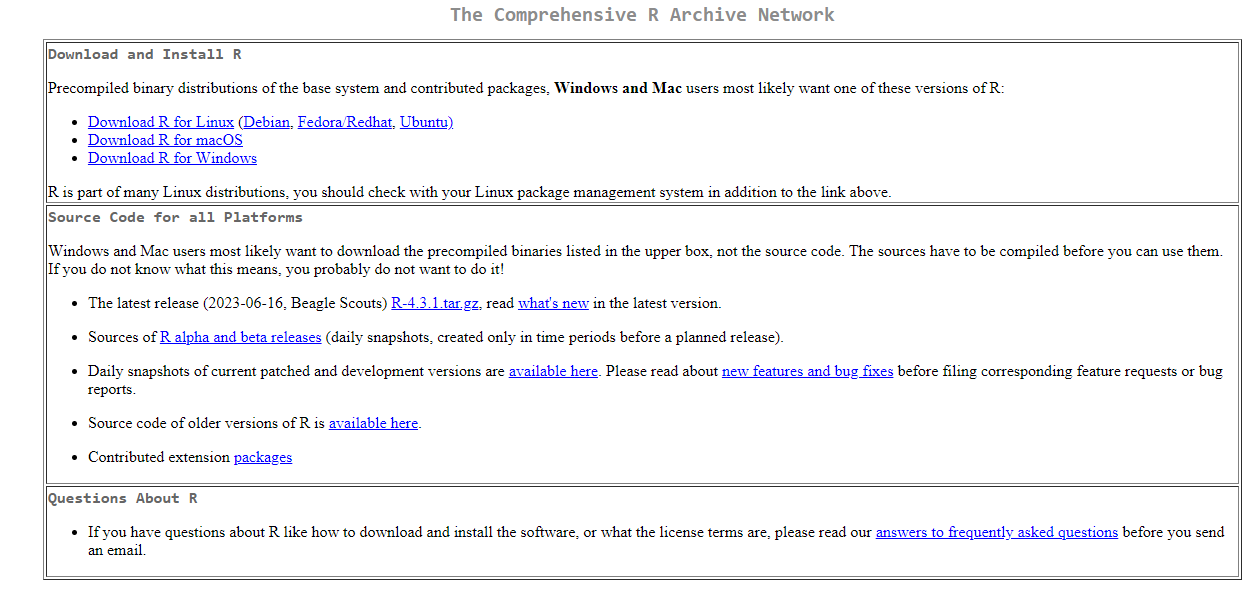
\includegraphics[width=6.91667in,height=4.11458in]{images/R download.PNG}
\item
  İndirilen sayfada \textbf{``base''} sekmesine tıklayın.

  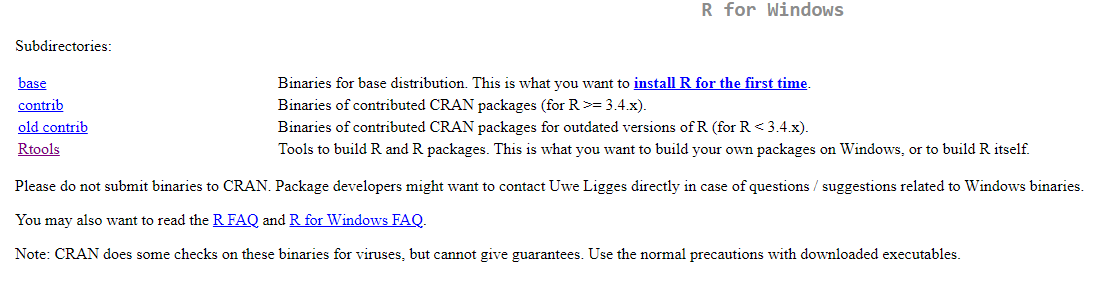
\includegraphics[width=6.90625in,height=2.79167in]{images/R download base.PNG}
\item
  Açılan sayfada ``Download R 4.3.1 for Windows'' linkine tıklayın ve
  dosyayı indirin.

  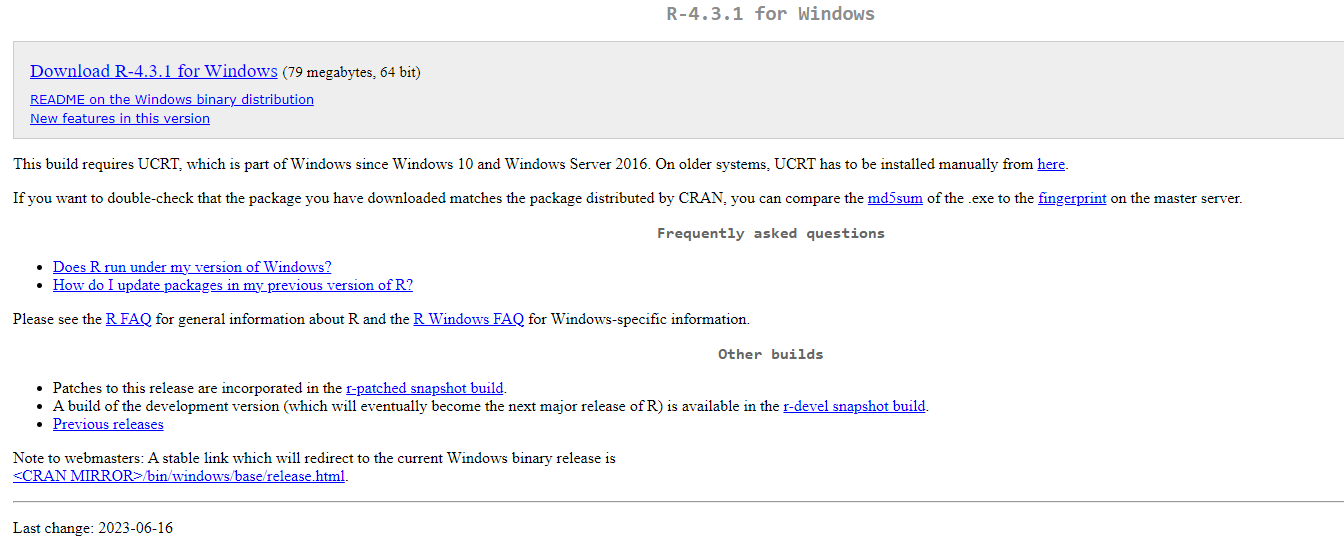
\includegraphics[width=6.8125in,height=3.5in]{images/R download win.PNG}

  \begin{tcolorbox}[enhanced jigsaw, titlerule=0mm, colbacktitle=quarto-callout-warning-color!10!white, leftrule=.75mm, colback=white, breakable, colframe=quarto-callout-warning-color-frame, bottomtitle=1mm, opacityback=0, left=2mm, title=\textcolor{quarto-callout-warning-color}{\faExclamationTriangle}\hspace{0.5em}{Dikkat}, rightrule=.15mm, opacitybacktitle=0.6, toptitle=1mm, arc=.35mm, bottomrule=.15mm, toprule=.15mm, coltitle=black]

  Sayfayı ziyaret ettiğiniz tarihlerde farklı sürümlerin olabileceğine
  dikkat edin. Örneğin ileri bir tarihte bu sayfayı ziyaret ettiğinizde
  R programının yeni sürümü ile karşılabilirsiniz. O yüzden sürüm
  bilgisi değişkenlik gösterebilir.

  \end{tcolorbox}
\item
  İndirilen dosyayı çift tıklayarak çalıştırın ve yükleyiciyi başlatın.
\item
  Yükleyici, R'nin temel sürümünü yüklemek için sizi yönlendirecektir.
  Varsayılan ayarları genellikle kabul edebilirsiniz.
\item
  Kurulum tamamlandığında, R'yi çalıştırmak için masaüstünüzde veya
  Başlat menüsünde \textbf{``R''} simgesini bulabilirsiniz.
\end{enumerate}

\textbf{Windows İşletim Sistemi İçin R Studio Kurulumu}

R editörü grafiksel bir arayüz olmayıp eski tip bir yazılım konsoludur.
\textbf{R Studio,} R programlama dili için geliştirilmiş entegre bir
geliştirme ortamı (IDE) ve arayüzüdür. R Studio, R kodlarını daha
verimli bir şekilde yazmanıza, çalıştırmanıza ve yönetmenize olanak
tanıyan daha modern ve kullanışlı bir arayüz sunmaktadır. Ayrıca veri
analizi, görselleştirme ve raporlama işlemleri için güçlü bir platform
sunar. R Studio, açık kaynak bir projedir ve ücretsiz olarak
kullanılabilir.

R Studio'nun kurulumu aşağıdaki adımlarla gerçekleştirilebilir:

\begin{enumerate}
\def\labelenumi{\arabic{enumi}.}
\item
  R Studio'nun en son sürümünü indirmek için aşağıdaki bağlantıyı
  kullanın:
  \href{https://www.rstudio.com/products/rstudio/download/}{\textbf{https://www.rstudio.com/products/rstudio/download/}}
\item
  Sayfada \textbf{``Download RStudio Desktop for Windows''} kısmına
  tıklayın ve indirmeyi başlatın.

  
\includegraphics[width=6.625in,height=4.02083in]{images/R Studio.PNG}
\item
  İndirilen dosyayı çift tıklayarak çalıştırın ve kurulumu başlatın.
  Kurulum sırasında varsayılan ayarları genellikle kabul edebilirsiniz.
\item
  Kurulum tamamlandığında, R Studio'yu başlatmak için masaüstünüzde veya
  Başlat menüsünde \textbf{``RStudio''} simgesini bulabilirsiniz.
\end{enumerate}

\section*{R Studio
Kişiselleştirme}\label{r-studio-kiux15fiselleux15ftirme}
\addcontentsline{toc}{section}{R Studio Kişiselleştirme}

\markright{R Studio Kişiselleştirme}

\pandocbounded{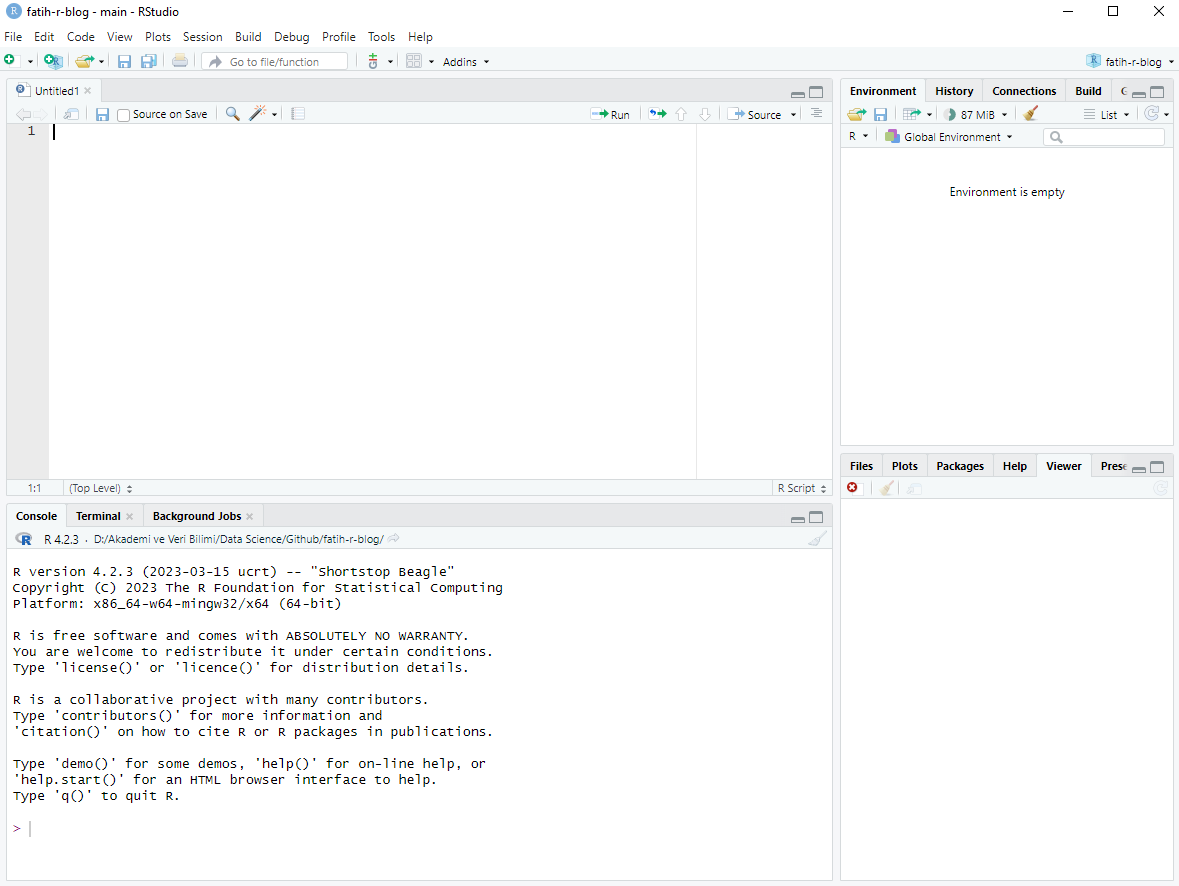
\includegraphics[keepaspectratio]{images/RStudio.PNG}}

RStudio, kullanıcıların ihtiyaçlarına göre kişiselleştirilebilen bir
entegre geliştirme ortamı (IDE) sunar. RStudio'yu kişiselleştirmek için
aşağıdaki yolları kullanabilirsiniz:

\begin{enumerate}
\def\labelenumi{\arabic{enumi}.}
\item
  \textbf{R Studio Arayüzündeki Alanları Değiştirme}: Resimde görüldüğü
  gibi yeni bir R Script açıldığı takdirde arayüzde 4 farklı alan
  görülmektedir. Bu alanlar isteğe göre yer değiştirilebilmektedir.
  Bunun için \textbf{``Tools''} (Araçlar) menüsünden \textbf{``Global
  Options''} (Genel Ayarlar) sekmesi açılır. Buradan \textbf{``Pane
  Layout''} kısmından istenilen ayarlar yapılabilir.
\item
  \textbf{Temayı ve Editör Stilini Değiştirme}: RStudio'nun görünümünü
  değiştirmek için birçok tema ve editör stilini seçebilirsiniz. Bu,
  yazılım geliştirme ortamınızın daha hoş veya kullanışlı olmasını
  sağlar. \textbf{``Tools''} (Araçlar) menüsünden \textbf{``Global
  Options''} (Genel Ayarlar) sekmesini seçerek bu ayarları
  değiştirebilirsiniz.
\item
  \textbf{Klavye Kısayollarını Kişiselleştirme}: RStudio'da kullanılan
  klavye kısayollarını özelleştirebilirsiniz. ``Tools'' (Araçlar)
  menüsünden ``Modify Keyboard Shortcuts'' (Klavye Kısayollarını
  Düzenle) seçeneğini kullanarak klavye kısayollarını tanımlayabilir
  veya değiştirebilirsiniz.
\item
  \textbf{Eklentileri ve Paketleri Kullanma}: RStudio, kullanıcıların
  işlevselliği genişletmek için eklentileri ve R paketlerini
  kullanmalarını sağlar. Bu paketler, kod otomatik tamamlama, kod
  görselleştirme, proje yönetimi gibi birçok işlemi kolaylaştırabilir. R
  Studio'nun sol üst köşesindeki \textbf{``Tools''} (Araçlar) menüsünden
  \textbf{``Install Packages''} (Paketleri Yükle) seçeneği ile yeni
  paketleri yükleyebilirsiniz.
\item
  \textbf{R Markdown Belgelerini Özelleştirme}: R Markdown belgeleri,
  raporlar ve belgeler oluşturmak için kullanılır. Bu belgeleri
  kişiselleştirebilirsiniz. R Markdown belgelerinin başlık, stil, tablo
  düzeni ve grafikler gibi birçok yönünü özelleştirebilirsiniz.
\item
  \textbf{Proje Ayarlarını Yapılandırma}: RStudio'da projeler kullanmak,
  projelerinizi daha düzenli ve etkili bir şekilde yönetmenize yardımcı
  olabilir. ``File'' (Dosya) menüsünden ``New Project'' (Yeni Proje)
  seçeneği ile yeni projeler oluşturabilir ve projelerinizi
  kişiselleştirebilirsiniz.
\item
  \textbf{Kod Tarayıcı ve Çalışma Ortamını Özelleştirme}: RStudio'nun
  sağ tarafında bulunan \textbf{``Environment''} (Çalışma Ortamı) ve
  \textbf{``Files''} (Dosyalar) sekmelerini özelleştirebilirsiniz. Bu
  sekmeleri dilediğiniz gibi düzenleyebilirsiniz.
\item
  \textbf{Addins Kullanma}: RStudio'nun ``Addins'' (Eklentiler) menüsü,
  kullanıcıların özel işlevleri ekleyebileceği bir bölümdür. Bu sayede
  belirli işlemleri hızlıca gerçekleştirebilirsiniz.
\end{enumerate}

RStudio'nun bu kişiselleştirme seçenekleri, kullanıcıların kendi
ihtiyaçlarına ve tercihlerine göre IDE'yi özelleştirmelerine olanak
tanır. Bu şekilde, RStudio'yu daha verimli ve kişiselleştirilmiş bir
şekilde kullanabilirsiniz. RStudio'nun ana bileşenleri ve temel
özellikleri ise şunlardır:

\begin{enumerate}
\def\labelenumi{\arabic{enumi}.}
\item
  \textbf{Script Editörü}: RStudio'nun sol üst kısmında yer alan bu
  bölüm, R kodlarını yazmak, düzenlemek ve çalıştırmak için kullanılır.
  Renk vurguları, otomatik tamamlama ve hata işaretleme gibi birçok
  yazılım geliştirme özelliği içerir.
\item
  \textbf{Environment (Çalışma Ortamı)} : Sağ üst köşede bulunan
  ``Çalışma Ortamı'' sekmesi, çalışan nesneleri ve değişkenleri
  görüntülemenizi sağlar. ``Files'' sekmesi ise projenizdeki dosyaları
  ve klasörleri görüntülemenize yardımcı olur.
\item
  \textbf{Console}: Alt sol köşede bulunan bu bölüm, R kodlarını anlık
  olarak çalıştırmanıza ve sonuçları görmesinize olanak tanır. R
  komutlarını doğrudan konsola yazabilir ve çalıştırabilirsiniz.
\item
  \textbf{Diğer Sekmeler} : RStudio, çeşitli grafikler ve
  görselleştirmeler oluşturmanıza olanak tanır. R koduyla çizilen
  grafikler, ``\textbf{Plots}'' sekmesinde görüntülenir. Bunu yanısıra
  ``\textbf{Help''} kısmında fonksiyonlar ile ilgili bilgi
  alınabilir,''\textbf{Packages''} kısmından ise paket yükleme vb. işler
  yapılabilir.
\end{enumerate}

\part{R Programlamaya Giriş}

R kodunun çalıştırılması oldukça basittir ve R Studio gibi entegre
geliştirme ortamları (IDE'ler) kullanırken daha da kolaylaşır. R kodunu
çalıştırmak için temel adımlar:

\begin{enumerate}
\def\labelenumi{\arabic{enumi}.}
\item
  \textbf{R Studio'yu Açın}: İlk adım, R Studio veya başka bir R
  IDE'sini açmaktır.
\item
  \textbf{Yeni Bir script uluşturun veya mevcut bir script kullanın}:

  \begin{itemize}
  \item
    R Studio'da, sol üst köşede bulunan ``File'' (Dosya) menüsünden
    ``New Script''seçeneği ile yeni bir R scripti oluşturabilirsiniz.
  \item
    Mevcut bir scripte gitmek istiyorsanız, ``File'' menüsünden ``Open
    Script'' seçeneğini kullanabilirsiniz.
  \end{itemize}
\item
  \textbf{R Kodunu Scripte Yazın}: Oluşturduğunuz veya açtığınız R
  skriptinde, R kodlarını yazın veya yapıştırın. Örneğin, basit bir
  hesaplama yapmak için aşağıdaki kodu kullanabilirsiniz:

\begin{Shaded}
\begin{Highlighting}[]
\NormalTok{x }\OtherTok{\textless{}{-}} \DecValTok{5}
\NormalTok{y }\OtherTok{\textless{}{-}} \DecValTok{10}
\NormalTok{z }\OtherTok{\textless{}{-}}\NormalTok{ x }\SpecialCharTok{+}\NormalTok{ y}
\NormalTok{z}
\end{Highlighting}
\end{Shaded}

\begin{verbatim}
[1] 15
\end{verbatim}
\item
  \textbf{Kodu Çalıştırma}:

  \begin{itemize}
  \item
    Çalıştırmak istediğiniz kodu seçin veya imleci çalıştırmak
    istediğiniz satıra getirin.
  \item
    Çalıştırma işlemi için aşağıdaki yöntemlerden birini
    kullanabilirsiniz:

    \begin{itemize}
    \item
      Klavyede varsayılan olarak ``Ctrl+Enter'' (Windows/Linux) veya
      ``Command+Enter'' (Mac) tuş kombinasyonunu kullanabilirsiniz.
    \item
      R Studio'daki ``Run'' (Çalıştır) düğmesini veya ``Run'' (Çalıştır)
      menüsünü kullanabilirsiniz.
    \item
      Çalıştırmak istediğiniz kodu seçtikten sonra sağ tıklarsanız,
      ``Run'' (Çalıştır) seçeneğini göreceksiniz.
    \end{itemize}
  \end{itemize}
\item
  \textbf{Sonuçları İnceleyin}: Çalıştırılan kodun sonuçları konsol
  penceresinde veya çıktı bölümünde görüntülenir. Örneğin, yukarıdaki
  örnekte ``z'' değişkeninin değeri olan ``15'' sonucunu göreceksiniz.
\end{enumerate}

\begin{tcolorbox}[enhanced jigsaw, titlerule=0mm, colbacktitle=quarto-callout-warning-color!10!white, leftrule=.75mm, colback=white, breakable, colframe=quarto-callout-warning-color-frame, bottomtitle=1mm, opacityback=0, left=2mm, title=\textcolor{quarto-callout-warning-color}{\faExclamationTriangle}\hspace{0.5em}{Dikkat}, rightrule=.15mm, opacitybacktitle=0.6, toptitle=1mm, arc=.35mm, bottomrule=.15mm, toprule=.15mm, coltitle=black]

Bir script üzerinden çalıştırılan R kodunun sonuçlarını sol alt kısımda
yer alan Console bölümünde görebilirsiniz. Aynı şekilde kodu Console
bölümüne yazıp Enter tuşuna bastığınızda yine sonuç alabilirsiniz. Ancak
script içerisinde yazılan kodları bir \textbf{\texttt{.R}} uzantılı
dosya olarak saklama ve daha sonradan bu dosyaya ulaşma şansınız varken,
Console ile çalıştırılan kodları bir \textbf{\texttt{.R}} dosyası olarak
saklama şansınız yoktur. Console tarafındaki sonuçlar geçici olarak
ekranda kalır ve R Studio'yu kapatıp açtığınızda tekrar yazdığınız ve
çalıştırdığınız kodlara ulaşamayabilirsiniz.

\end{tcolorbox}

\begin{tcolorbox}[enhanced jigsaw, titlerule=0mm, colbacktitle=quarto-callout-tip-color!10!white, leftrule=.75mm, colback=white, breakable, colframe=quarto-callout-tip-color-frame, bottomtitle=1mm, opacityback=0, left=2mm, title=\textcolor{quarto-callout-tip-color}{\faLightbulb}\hspace{0.5em}{İpucu}, rightrule=.15mm, opacitybacktitle=0.6, toptitle=1mm, arc=.35mm, bottomrule=.15mm, toprule=.15mm, coltitle=black]

Console tarafına yansıyan kodların ve sonuçların farklı formatlarda
saklama şansımız vardır. Bunun için \texttt{sink} fonksiyonunu
araştırmanızı önerebilirim.

\end{tcolorbox}

\chapter{Temel Fonksiyonlar}\label{temel-fonksiyonlar}

\section{Çalışma Dizini}\label{uxe7alux131ux15fma-dizini}

Çalışma Dizini, üzerinde çalıştığınız projenin tüm gerekli dosya ve
belgelerini içerdiği yerdir. Çalışma dizininizi ayarlamanın iki yolu
vardır. İlk yol \ul{\textbf{getwd ve setwd}} işlevlerini kullanmaktır.
Diğer yol ise RStudio üzerinden \ul{\textbf{Session\textgreater Set
Working Directory}} youluyla yapılabilir.

\begin{Shaded}
\begin{Highlighting}[]
\FunctionTok{getwd}\NormalTok{()}
\end{Highlighting}
\end{Shaded}

\begin{itemize}
\item
  \ul{\textbf{\mbox{\texttt{dir}}}} veya
  \ul{\textbf{\mbox{\texttt{list.files}}}} komutları ile dizinde yer
  alan dosyalar öğrenilebilir.
\item
  \ul{\textbf{\mbox{\texttt{dir.create}}}} komutu ile yeni bir klasör
  oluşturmak mümkündür.
\item
  \ul{\textbf{\mbox{\texttt{file.exists}}}} kullanılarak klasörün var
  olup olmadığı sorgulanabilir.
\end{itemize}

\section{Yardımcı Bilgiler}\label{yardux131mcux131-bilgiler}

\textbf{R} komutlarında \emph{Büyük-küçük harf duyarlılığı (case
sensitive)} vardır.

\begin{Shaded}
\begin{Highlighting}[]
\NormalTok{a }\OtherTok{\textless{}{-}} \DecValTok{5}  
\FunctionTok{print}\NormalTok{(a)  }
\end{Highlighting}
\end{Shaded}

\begin{verbatim}
[1] 5
\end{verbatim}

\begin{Shaded}
\begin{Highlighting}[]
\NormalTok{A }\OtherTok{\textless{}{-}} \DecValTok{6}  
\FunctionTok{print}\NormalTok{(A) }
\end{Highlighting}
\end{Shaded}

\begin{verbatim}
[1] 6
\end{verbatim}

\textbf{Noktalı virgül (;)} işareti ile aynı satırda birden fazla kod
çalıştırılabilir hale getirilir.

\begin{Shaded}
\begin{Highlighting}[]
\NormalTok{x }\OtherTok{\textless{}{-}} \DecValTok{1}\NormalTok{ ; y }\OtherTok{\textless{}{-}} \DecValTok{2}\NormalTok{ ; z }\OtherTok{\textless{}{-}} \DecValTok{3}  
\NormalTok{x; y; z}
\end{Highlighting}
\end{Shaded}

\begin{verbatim}
[1] 1
\end{verbatim}

\begin{verbatim}
[1] 2
\end{verbatim}

\begin{verbatim}
[1] 3
\end{verbatim}

Komutlar arası açıklamaları ve yorumları \textbf{\#(hashtag)} ile
yazabiliriz. Hastagli satırlar, kod olarak algılanıp çalıştırılmaz. Bu
kısımlara yazılan kodlar ile ilgili hatırlatıcı bilgiler (comment)
yazılabilir.

\begin{Shaded}
\begin{Highlighting}[]
\CommentTok{\#6 ile başyalan ve  10 ile  biten tamsayıları c vektörüne atayalım  }
\NormalTok{c }\OtherTok{\textless{}{-}} \DecValTok{6}\SpecialCharTok{:}\DecValTok{10} 
\NormalTok{c}
\end{Highlighting}
\end{Shaded}

\begin{verbatim}
[1]  6  7  8  9 10
\end{verbatim}

\begin{itemize}
\item
  \textbf{\texttt{ls()}} çalışma alanındaki nesne ve fonksiyonları
  listeler.
\item
  \textbf{\texttt{rm(a)}} çalışma alanından \textbf{a} nesnesini siler.
\item
  \textbf{\texttt{rm(list=ls())}} bütün çalışma alanını temizler.
\item
  \textbf{\texttt{q()}} R'dan çıkış yapmayı sağlar.
\item
  \textbf{\texttt{install.packages("package")}} paket yüklemeyi sağlar.
\item
  \textbf{\texttt{library("package")}} yüklü olan paketi getirir.
\item
  \textbf{\texttt{installed.packages()}} yüklü olan paketleri listeler
\item
  \textbf{\texttt{options(digits=10)}} sayılarda ondalık kısmın basamak
  sayısını ifade eder.
\item
  \textbf{\texttt{help()}} fonksiyonu ya da \textbf{\texttt{?}} ile bir
  fonksiyon hakkında yardım alınabilir. Örneğin mean fonksiyonu ile
  ilgili yardım almak için scripte \texttt{?mean} ya da help(mean)
  yazmanız ve çalıştırmanız yeterlidir. Bunun yanı sıra R Studio
  penceresinin sağ alt kısmındaki help alanını kullanabilirsiniz.
\end{itemize}

\section{Atama Operatörü}\label{atama-operatuxf6ruxfc}

Bir değişkene, tabloya veya objeye değer atarken \textbf{`\textless-'}
veya \textbf{`='} operatörü kullanılır. `\textbf{\textless-}' atama
operatöründe ok hangi yöndeyse o tarafa atama yapılır. Genellikle
`\textbf{\textless-}' operatörü kullanılmaktadır. Çünkü `\textbf{=}'
operatörü filtrelemelerde veya işlemlerdeki `\textbf{==}' ile
karıştırılabilmektedir. Ayrıca fonksiyonlar içinde de kullanılabildiği
için kod karmaşasına sebebiyet verebilir. Her iki operatör de aynı
işlevi görmektedir.

\begin{Shaded}
\begin{Highlighting}[]
\CommentTok{\# a\textquotesingle{}ya 20 değerini atayalım  }
\NormalTok{a }\OtherTok{\textless{}{-}} \DecValTok{20}    
\CommentTok{\# tabloyu ya da değeri görüntülemek için nesnenin kendisi de direkt yazılabilir.  }
\CommentTok{\# ya da print fonksiyonu kullanılabilir.   }
\FunctionTok{print}\NormalTok{(a)    }
\end{Highlighting}
\end{Shaded}

\begin{verbatim}
[1] 20
\end{verbatim}

\begin{Shaded}
\begin{Highlighting}[]
\CommentTok{\# b\textquotesingle{}ye 12 değerini atayalım  }
\NormalTok{b }\OtherTok{\textless{}{-}} \DecValTok{12}  
\FunctionTok{print}\NormalTok{(b)   }
\end{Highlighting}
\end{Shaded}

\begin{verbatim}
[1] 12
\end{verbatim}

\begin{Shaded}
\begin{Highlighting}[]
\CommentTok{\# a ve b değerlerinden üretilen bir c değeri üretelim.   }
\NormalTok{c }\OtherTok{\textless{}{-}} \DecValTok{2} \SpecialCharTok{*}\NormalTok{ a }\SpecialCharTok{+} \DecValTok{3} \SpecialCharTok{*}\NormalTok{ b  }
\FunctionTok{print}\NormalTok{(c) }
\end{Highlighting}
\end{Shaded}

\begin{verbatim}
[1] 76
\end{verbatim}

\textbf{c()} ile vektör oluştutulabilir. c ``combine'' (birleştirmek)
kelimesinin ilk harfini ifade eder. Bir değişkene birden fazla değer
atamak istediğimizde kullanılır.

\begin{Shaded}
\begin{Highlighting}[]
\CommentTok{\# d adında bir vektör oluşturalım ve değerler atayalım.   }
\NormalTok{d }\OtherTok{\textless{}{-}} \FunctionTok{c}\NormalTok{(}\DecValTok{4}\NormalTok{,}\DecValTok{7}\NormalTok{,}\DecValTok{13}\NormalTok{)  }
\NormalTok{d }
\end{Highlighting}
\end{Shaded}

\begin{verbatim}
[1]  4  7 13
\end{verbatim}

Bir metini değişkene atamak istersek de aşağıdaki gibi metin ``\,''
işareti içine yazılmalıdır.

\begin{Shaded}
\begin{Highlighting}[]
\NormalTok{metin }\OtherTok{\textless{}{-}} \StringTok{"Merhaba Arkadaşlar"}  
\FunctionTok{print}\NormalTok{(metin)}
\end{Highlighting}
\end{Shaded}

\begin{verbatim}
[1] "Merhaba Arkadaşlar"
\end{verbatim}

\section{Matematiksel Operatörler}\label{matematiksel-operatuxf6rler}

R ve R Studio, güçlü bir hesap makinesi olarak kabul edilebilir.

\begin{Shaded}
\begin{Highlighting}[]
\DecValTok{3}\SpecialCharTok{+}\DecValTok{5} 
\end{Highlighting}
\end{Shaded}

\begin{verbatim}
[1] 8
\end{verbatim}

\begin{Shaded}
\begin{Highlighting}[]
\DecValTok{7}\SpecialCharTok{*}\DecValTok{8} 
\end{Highlighting}
\end{Shaded}

\begin{verbatim}
[1] 56
\end{verbatim}

\begin{Shaded}
\begin{Highlighting}[]
\DecValTok{88}\SpecialCharTok{/}\DecValTok{2} 
\end{Highlighting}
\end{Shaded}

\begin{verbatim}
[1] 44
\end{verbatim}

\begin{Shaded}
\begin{Highlighting}[]
\DecValTok{3}\SpecialCharTok{*}\NormalTok{(}\DecValTok{12}\SpecialCharTok{+}\NormalTok{(}\DecValTok{15}\SpecialCharTok{/}\DecValTok{3{-}2}\NormalTok{)) }
\end{Highlighting}
\end{Shaded}

\begin{verbatim}
[1] 45
\end{verbatim}

\begin{Shaded}
\begin{Highlighting}[]
\DecValTok{9}\SpecialCharTok{\^{}}\DecValTok{2} \CommentTok{\# karesini alır }
\end{Highlighting}
\end{Shaded}

\begin{verbatim}
[1] 81
\end{verbatim}

\begin{Shaded}
\begin{Highlighting}[]
\NormalTok{a }\OtherTok{\textless{}{-}}  \DecValTok{3} 
\NormalTok{b }\OtherTok{\textless{}{-}}\NormalTok{  a}\SpecialCharTok{\^{}}\DecValTok{2} 
\FunctionTok{print}\NormalTok{(b) }
\end{Highlighting}
\end{Shaded}

\begin{verbatim}
[1] 9
\end{verbatim}

\begin{Shaded}
\begin{Highlighting}[]
\FunctionTok{log}\NormalTok{(}\DecValTok{15}\NormalTok{) }\CommentTok{\#ln15 yani doğal logaritma }
\end{Highlighting}
\end{Shaded}

\begin{verbatim}
[1] 2.70805
\end{verbatim}

\begin{Shaded}
\begin{Highlighting}[]
\FunctionTok{log10}\NormalTok{(}\DecValTok{1000}\NormalTok{) }\CommentTok{\# 10 tabanına göre hesaplama }
\end{Highlighting}
\end{Shaded}

\begin{verbatim}
[1] 3
\end{verbatim}

\begin{Shaded}
\begin{Highlighting}[]
\FunctionTok{exp}\NormalTok{(}\DecValTok{12}\NormalTok{) }\CommentTok{\#exponential power of the number. e (2.718) üzeri 12 }
\end{Highlighting}
\end{Shaded}

\begin{verbatim}
[1] 162754.8
\end{verbatim}

\begin{Shaded}
\begin{Highlighting}[]
\FunctionTok{factorial}\NormalTok{(}\DecValTok{6}\NormalTok{) }\CommentTok{\# faktöriyel hesaplama yapar }
\end{Highlighting}
\end{Shaded}

\begin{verbatim}
[1] 720
\end{verbatim}

\begin{Shaded}
\begin{Highlighting}[]
\FunctionTok{sqrt}\NormalTok{(}\DecValTok{81}\NormalTok{) }\CommentTok{\# karekök alma }
\end{Highlighting}
\end{Shaded}

\begin{verbatim}
[1] 9
\end{verbatim}

\begin{Shaded}
\begin{Highlighting}[]
\FunctionTok{abs}\NormalTok{(}\SpecialCharTok{{-}}\DecValTok{3}\NormalTok{) }\CommentTok{\# mutlak değer }
\end{Highlighting}
\end{Shaded}

\begin{verbatim}
[1] 3
\end{verbatim}

\begin{Shaded}
\begin{Highlighting}[]
\FunctionTok{sign}\NormalTok{(}\SpecialCharTok{{-}}\DecValTok{5}\NormalTok{) }\CommentTok{\# işaret bulma }
\end{Highlighting}
\end{Shaded}

\begin{verbatim}
[1] -1
\end{verbatim}

\begin{Shaded}
\begin{Highlighting}[]
\FunctionTok{sin}\NormalTok{(}\DecValTok{45}\NormalTok{) }\CommentTok{\# sinüs }
\end{Highlighting}
\end{Shaded}

\begin{verbatim}
[1] 0.8509035
\end{verbatim}

\begin{Shaded}
\begin{Highlighting}[]
\FunctionTok{cos}\NormalTok{(}\DecValTok{90}\NormalTok{) }\CommentTok{\# cosinüs }
\end{Highlighting}
\end{Shaded}

\begin{verbatim}
[1] -0.4480736
\end{verbatim}

\begin{Shaded}
\begin{Highlighting}[]
\NormalTok{pi }\CommentTok{\# pi sayısı }
\end{Highlighting}
\end{Shaded}

\begin{verbatim}
[1] 3.141593
\end{verbatim}

\begin{Shaded}
\begin{Highlighting}[]
\FunctionTok{tan}\NormalTok{(pi) }\CommentTok{\# tanjant}
\end{Highlighting}
\end{Shaded}

\begin{verbatim}
[1] -1.224647e-16
\end{verbatim}

\section{Mantıksal Operatörler}\label{mantux131ksal-operatuxf6rler}

Mantıksal sorgulamalar, koşullarda ve filtrelerde kullanılmaktadır.
Verilen koşul veya filtre sağlandığında \textbf{TRUE}, sağlanmadığında
ise \textbf{FALSE} değerleri elde edilmektedir. Bu mantıksal operatörler
ayrıca komutlar içindeki özellikleri aktifleştirmek ve pasifleştirmek
için de kullanılmaktadır.

Mantıksal operatörler aşağıdaki şekilde kullanılmaktadır:

\begin{itemize}
\item
  eşittir : \textbf{==}
\item
  eşit değildir : \textbf{!=}
\item
  küçüktür : \textbf{\textless{}}
\item
  küçük eşittir : \textbf{\textless=}
\item
  büyüktür : \textbf{\textgreater{}}
\item
  büyük eşittir : \textbf{\textgreater=}
\item
  x değil : \textbf{!x}
\item
  x ve y : \textbf{x\&y}
\item
  x veya y: \textbf{x\textbar y}
\end{itemize}

\begin{Shaded}
\begin{Highlighting}[]
\DecValTok{3} \SpecialCharTok{\textgreater{}} \DecValTok{5}
\end{Highlighting}
\end{Shaded}

\begin{verbatim}
[1] FALSE
\end{verbatim}

\begin{Shaded}
\begin{Highlighting}[]
\CommentTok{\# \& (ve) operatörü}
\CommentTok{\# iki durumda TRUE ise sonuç TRUE döner.}
\DecValTok{3} \SpecialCharTok{\textless{}} \DecValTok{5} \SpecialCharTok{\&} \DecValTok{8} \SpecialCharTok{\textgreater{}} \DecValTok{7}
\end{Highlighting}
\end{Shaded}

\begin{verbatim}
[1] TRUE
\end{verbatim}

\begin{Shaded}
\begin{Highlighting}[]
\CommentTok{\# bir durum FALSE diğer durum TRUE ise sonuç FALSE döner.}
\DecValTok{3} \SpecialCharTok{\textless{}} \DecValTok{5} \SpecialCharTok{\&} \DecValTok{6} \SpecialCharTok{\textgreater{}} \DecValTok{7}
\end{Highlighting}
\end{Shaded}

\begin{verbatim}
[1] FALSE
\end{verbatim}

\begin{Shaded}
\begin{Highlighting}[]
\CommentTok{\# iki durumda FALSE ise sonuç FALSE döner.}
\DecValTok{6} \SpecialCharTok{\textless{}} \DecValTok{5} \SpecialCharTok{\&} \DecValTok{6} \SpecialCharTok{\textgreater{}} \DecValTok{7}
\end{Highlighting}
\end{Shaded}

\begin{verbatim}
[1] FALSE
\end{verbatim}

\begin{Shaded}
\begin{Highlighting}[]
\CommentTok{\# | (veya) operatörü}
\CommentTok{\# Her iki durumdan birisi TRUE ise TRUE döner}
\NormalTok{(}\DecValTok{5}\SpecialCharTok{==}\DecValTok{4}\NormalTok{) }\SpecialCharTok{|}\NormalTok{ (}\DecValTok{3}\SpecialCharTok{!=}\DecValTok{4}\NormalTok{)}
\end{Highlighting}
\end{Shaded}

\begin{verbatim}
[1] TRUE
\end{verbatim}

\chapter{Veri Tipleri ve
Yapıları}\label{veri-tipleri-ve-yapux131larux131}

\section{Veri Tipleri}\label{veri-tipleri}

R'da kulllanılan 5 farklı veri tipi vardır. Bu veri tipleri atomic
vectörler olarak da bilinir. Atomic olması vektörlerin homojen olması
anlamına gelmektedir. Yani vektör içerisinde aynı veri tipinden değerler
yer alabilir. Veri tipleri;

\begin{itemize}
\item
  numeric veya double (reel sayılar)
\item
  integer (tamsayılar)
\item
  complex (karmaşık sayılar)
\item
  character (metinsel ifadeler)
\item
  logical, TRUE ve FALSE (mantıksal)
\end{itemize}

\texttt{typeof()} veya \texttt{class()} fonksiyonları ile veri tipi
öğrenilebilir.

\begin{tcolorbox}[enhanced jigsaw, titlerule=0mm, colbacktitle=quarto-callout-important-color!10!white, leftrule=.75mm, colback=white, breakable, colframe=quarto-callout-important-color-frame, bottomtitle=1mm, opacityback=0, left=2mm, title=\textcolor{quarto-callout-important-color}{\faExclamation}\hspace{0.5em}{Önemli}, rightrule=.15mm, opacitybacktitle=0.6, toptitle=1mm, arc=.35mm, bottomrule=.15mm, toprule=.15mm, coltitle=black]

\textbf{\texttt{typeof()}} ve \textbf{\texttt{class()}} fonksiyonları, R
programlama dilinde nesnelerin özelliklerini sorgulamak için kullanılır.
Farklı amaçlara hizmet ederler ve bazı durumlarda farklı sonuçlar
üretebilirler.

\begin{itemize}
\item
  \textbf{\texttt{typeof()}} fonksiyonu, bir nesnenin temel veri türünü
  belirler. Örneğin, bir nesnenin karakter dizisi (string), sayı, liste,
  fonksiyon veya vektör gibi temel veri türlerinden hangisine ait
  olduğunu gösterir. Ancak, nesnenin özel sınıfını (class) ifade etmez.
  Örneğin, bir faktörün \textbf{\texttt{typeof()}} değeri ``integer''
  olabilir.
\item
  \textbf{\texttt{class()}} fonksiyonu ise bir nesnenin özel sınıfını
  belirtir. Eğer bir nesne özel bir sınıfa aitse (örneğin, bir veri
  çerçevesi veya faktör), \textbf{\texttt{class()}} fonksiyonu bu özel
  sınıfın adını verir. Eğer nesne birden fazla sınıfa aitse, sınıflar
  bir sıra halinde listelenir.
\end{itemize}

Bu fonksiyonlar genellikle birlikte kullanılır çünkü bir nesnenin veri
tipi ve sınıfı arasında farklılıklar olabilir. Örneğin, bir veri
çerçevesi \textbf{\texttt{typeof()}} ile incelendiğinde
\textbf{\texttt{list}} çıkabilir, çünkü veri çerçeveleri bir liste
türündedir. Ancak, \textbf{\texttt{class()}} fonksiyonu bu nesnenin özel
sınıfını, yani \textbf{\texttt{data.frame}} olarak gösterecektir. Bu
farklılıklar, bir nesnenin hangi özelliklere sahip olduğunu daha iyi
anlamak için kullanılabilir.

\end{tcolorbox}

\textbf{numeric}

\begin{Shaded}
\begin{Highlighting}[]
\NormalTok{a }\OtherTok{\textless{}{-}} \FloatTok{3.5}
\FunctionTok{class}\NormalTok{(a)}
\end{Highlighting}
\end{Shaded}

\begin{verbatim}
[1] "numeric"
\end{verbatim}

\begin{Shaded}
\begin{Highlighting}[]
\FunctionTok{typeof}\NormalTok{(a) }\CommentTok{\# typeof numeriklerin tipini double olarak gösterir.}
\end{Highlighting}
\end{Shaded}

\begin{verbatim}
[1] "double"
\end{verbatim}

\begin{Shaded}
\begin{Highlighting}[]
\FunctionTok{is.numeric}\NormalTok{(a) }\CommentTok{\# verinin tipinin numerik olup olmadığı sorgulanır.}
\end{Highlighting}
\end{Shaded}

\begin{verbatim}
[1] TRUE
\end{verbatim}

\textbf{integer}

\begin{Shaded}
\begin{Highlighting}[]
\NormalTok{b }\OtherTok{\textless{}{-}} \DecValTok{5}
\FunctionTok{class}\NormalTok{(b)}
\end{Highlighting}
\end{Shaded}

\begin{verbatim}
[1] "numeric"
\end{verbatim}

\begin{Shaded}
\begin{Highlighting}[]
\FunctionTok{is.integer}\NormalTok{(b)}
\end{Highlighting}
\end{Shaded}

\begin{verbatim}
[1] FALSE
\end{verbatim}

\begin{Shaded}
\begin{Highlighting}[]
\NormalTok{c }\OtherTok{\textless{}{-}} \DecValTok{6}\NormalTok{L }\CommentTok{\# integer olması için sayının sağına L yazılır.}
\FunctionTok{class}\NormalTok{(c)}
\end{Highlighting}
\end{Shaded}

\begin{verbatim}
[1] "integer"
\end{verbatim}

\begin{Shaded}
\begin{Highlighting}[]
\FunctionTok{is.integer}\NormalTok{(c)}
\end{Highlighting}
\end{Shaded}

\begin{verbatim}
[1] TRUE
\end{verbatim}

\begin{Shaded}
\begin{Highlighting}[]
\FunctionTok{class}\NormalTok{(}\FunctionTok{as.integer}\NormalTok{(b)) }\CommentTok{\# as. ile baslayan fonksiyonlar dönüşüm için kullanılır.}
\end{Highlighting}
\end{Shaded}

\begin{verbatim}
[1] "integer"
\end{verbatim}

\textbf{complex}

\begin{Shaded}
\begin{Highlighting}[]
\NormalTok{z }\OtherTok{\textless{}{-}} \DecValTok{4} \SpecialCharTok{+} \DecValTok{2}\NormalTok{i}
\FunctionTok{class}\NormalTok{(z)}
\end{Highlighting}
\end{Shaded}

\begin{verbatim}
[1] "complex"
\end{verbatim}

\textbf{character}

\begin{Shaded}
\begin{Highlighting}[]
\NormalTok{d }\OtherTok{\textless{}{-}} \StringTok{"R Programlama"}
\FunctionTok{class}\NormalTok{(d)}
\end{Highlighting}
\end{Shaded}

\begin{verbatim}
[1] "character"
\end{verbatim}

\begin{Shaded}
\begin{Highlighting}[]
\NormalTok{e }\OtherTok{\textless{}{-}} \StringTok{"5.5"}
\FunctionTok{class}\NormalTok{(e)}
\end{Highlighting}
\end{Shaded}

\begin{verbatim}
[1] "character"
\end{verbatim}

\begin{Shaded}
\begin{Highlighting}[]
\FunctionTok{class}\NormalTok{(}\FunctionTok{as.numeric}\NormalTok{(e))}
\end{Highlighting}
\end{Shaded}

\begin{verbatim}
[1] "numeric"
\end{verbatim}

\textbf{logical}

\begin{Shaded}
\begin{Highlighting}[]
\NormalTok{x }\OtherTok{\textless{}{-}} \ConstantTok{TRUE}
\NormalTok{y }\OtherTok{\textless{}{-}} \ConstantTok{FALSE}
\FunctionTok{class}\NormalTok{(}\FunctionTok{c}\NormalTok{(x,y))}
\end{Highlighting}
\end{Shaded}

\begin{verbatim}
[1] "logical"
\end{verbatim}

\begin{Shaded}
\begin{Highlighting}[]
\FunctionTok{as.integer}\NormalTok{(}\FunctionTok{c}\NormalTok{(x,y)) }\CommentTok{\# TRUE ve FALSE numeric olarak 1 ve 0 değerine karşılık gelir.}
\end{Highlighting}
\end{Shaded}

\begin{verbatim}
[1] 1 0
\end{verbatim}

\section{Veri Yapıları}\label{veri-yapux131larux131}

\begin{figure}[H]

{\centering \pandocbounded{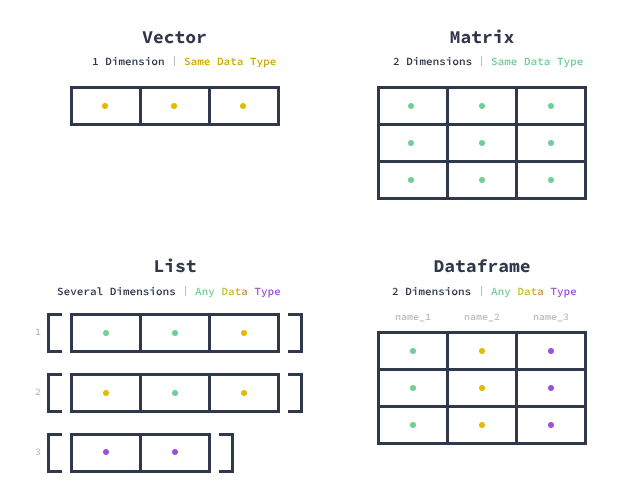
\includegraphics[keepaspectratio]{images/data_structures.png}}

}

\caption{https://app.dataquest.io/m/493/dataframes-in-r/1/introduction}

\end{figure}%

\subsection{Vektörler}\label{vektuxf6rler}

\begin{itemize}
\item
  R'daki en temel nesneler vektörlerdir.
\item
  Vektörler homojen yapıya sahiptir yani bütün elemanları aynı veri
  tipinde olmalıdır.
\item
  Vektörler tek boyutludur.
\item
  Bir vektör oluşturmak için kullanabilecek en temel fonksiyon
  \textbf{\texttt{c()}}'dir.
\end{itemize}

\begin{Shaded}
\begin{Highlighting}[]
\NormalTok{v }\OtherTok{\textless{}{-}} \FunctionTok{c}\NormalTok{(}\DecValTok{1}\NormalTok{,}\DecValTok{4}\NormalTok{,}\DecValTok{7}\NormalTok{,}\DecValTok{2}\NormalTok{,}\DecValTok{5}\NormalTok{,}\DecValTok{8}\NormalTok{,}\DecValTok{3}\NormalTok{,}\DecValTok{6}\NormalTok{,}\DecValTok{9}\NormalTok{)}

\NormalTok{v[}\DecValTok{1}\NormalTok{] }\CommentTok{\# 1. elemanını seçer}
\end{Highlighting}
\end{Shaded}

\begin{verbatim}
[1] 1
\end{verbatim}

\begin{Shaded}
\begin{Highlighting}[]
\NormalTok{v[}\DecValTok{3}\NormalTok{] }\CommentTok{\# 3. elemanını seçer}
\end{Highlighting}
\end{Shaded}

\begin{verbatim}
[1] 7
\end{verbatim}

\begin{Shaded}
\begin{Highlighting}[]
\NormalTok{v[}\FunctionTok{c}\NormalTok{(}\DecValTok{3}\NormalTok{,}\DecValTok{7}\NormalTok{)] }\CommentTok{\# 3. ve 7. elemani secer}
\end{Highlighting}
\end{Shaded}

\begin{verbatim}
[1] 7 3
\end{verbatim}

\begin{Shaded}
\begin{Highlighting}[]
\NormalTok{v[}\DecValTok{1}\SpecialCharTok{:}\DecValTok{6}\NormalTok{] }\CommentTok{\# 1. elemandan 6. elemana kadar secer}
\end{Highlighting}
\end{Shaded}

\begin{verbatim}
[1] 1 4 7 2 5 8
\end{verbatim}

\begin{Shaded}
\begin{Highlighting}[]
\NormalTok{v[}\SpecialCharTok{{-}}\DecValTok{2}\NormalTok{] }\CommentTok{\# 2. elemani haric tutarak secer}
\end{Highlighting}
\end{Shaded}

\begin{verbatim}
[1] 1 7 2 5 8 3 6 9
\end{verbatim}

\begin{Shaded}
\begin{Highlighting}[]
\FunctionTok{length}\NormalTok{(v) }\CommentTok{\# vektörün uzunluğunu gösterir}
\end{Highlighting}
\end{Shaded}

\begin{verbatim}
[1] 9
\end{verbatim}

\begin{Shaded}
\begin{Highlighting}[]
\NormalTok{v2 }\OtherTok{\textless{}{-}} \FunctionTok{c}\NormalTok{(v,}\DecValTok{12}\NormalTok{) }\CommentTok{\# vektöre eleman ekleme}
\NormalTok{v2}
\end{Highlighting}
\end{Shaded}

\begin{verbatim}
 [1]  1  4  7  2  5  8  3  6  9 12
\end{verbatim}

\begin{Shaded}
\begin{Highlighting}[]
\CommentTok{\# : ile başlangıç ve bitiş değerleri belli olan vektörler yaratılabilir.}

\NormalTok{v3 }\OtherTok{\textless{}{-}} \DecValTok{1}\SpecialCharTok{:}\DecValTok{10}
\NormalTok{v3}
\end{Highlighting}
\end{Shaded}

\begin{verbatim}
 [1]  1  2  3  4  5  6  7  8  9 10
\end{verbatim}

\begin{Shaded}
\begin{Highlighting}[]
\NormalTok{v4 }\OtherTok{\textless{}{-}} \DecValTok{11}\SpecialCharTok{:}\DecValTok{20}
\NormalTok{v4}
\end{Highlighting}
\end{Shaded}

\begin{verbatim}
 [1] 11 12 13 14 15 16 17 18 19 20
\end{verbatim}

\begin{Shaded}
\begin{Highlighting}[]
\CommentTok{\# Vektörler ile matematiksel işlemler yapılabilir.}

\NormalTok{v3 }\SpecialCharTok{+}\NormalTok{ v4}
\end{Highlighting}
\end{Shaded}

\begin{verbatim}
 [1] 12 14 16 18 20 22 24 26 28 30
\end{verbatim}

\begin{Shaded}
\begin{Highlighting}[]
\NormalTok{v3 }\SpecialCharTok{/}\NormalTok{ v4}
\end{Highlighting}
\end{Shaded}

\begin{verbatim}
 [1] 0.09090909 0.16666667 0.23076923 0.28571429 0.33333333 0.37500000
 [7] 0.41176471 0.44444444 0.47368421 0.50000000
\end{verbatim}

\begin{Shaded}
\begin{Highlighting}[]
\DecValTok{2} \SpecialCharTok{*}\NormalTok{ v3 }\SpecialCharTok{{-}}\NormalTok{ v4}
\end{Highlighting}
\end{Shaded}

\begin{verbatim}
 [1] -9 -8 -7 -6 -5 -4 -3 -2 -1  0
\end{verbatim}

Aşağıda vektörler ile birlikte sıklıkla kulanılan bazı fonksiyonlara yer
verilmiştir.

\subsubsection{\texorpdfstring{\textbf{seq}}{seq}}\label{seq}

\textbf{\texttt{seq()}} fonksiyonu, ardışık sayı dizileri oluşturmak
için kullanılır. Bu fonksiyon, başlangıç ve bitiş değerlerinin yanı sıra
belirli bir artış veya azalış miktarını belirterek ardışık bir dizi
oluşturmanızı sağlar.

\textbf{\texttt{seq()}} fonksiyonu genellikle üç temel parametre alır:

\begin{enumerate}
\def\labelenumi{\arabic{enumi}.}
\item
  \textbf{\texttt{from}}: Dizinin başlangıç değeri.
\item
  \textbf{\texttt{to}}: Dizinin bitiş değeri.
\item
  \textbf{\texttt{by}}: Opsiyonel olarak belirlenebilen artış/azalış
  miktarı.
\end{enumerate}

\begin{Shaded}
\begin{Highlighting}[]
\FunctionTok{seq}\NormalTok{(}\AttributeTok{from =} \DecValTok{5}\NormalTok{, }\AttributeTok{to =} \DecValTok{50}\NormalTok{, }\AttributeTok{by =}\DecValTok{5}\NormalTok{) }\CommentTok{\# 5 ile başlayan 50 ile biten 5şer artan vektör}
\end{Highlighting}
\end{Shaded}

\begin{verbatim}
 [1]  5 10 15 20 25 30 35 40 45 50
\end{verbatim}

\begin{Shaded}
\begin{Highlighting}[]
\FunctionTok{seq}\NormalTok{(}\AttributeTok{from =} \DecValTok{5}\NormalTok{, }\AttributeTok{to =} \DecValTok{50}\NormalTok{, }\AttributeTok{length =} \DecValTok{7}\NormalTok{) }\CommentTok{\# 5 ile başlayan 50 ile 7 elemanlı vektör}
\end{Highlighting}
\end{Shaded}

\begin{verbatim}
[1]  5.0 12.5 20.0 27.5 35.0 42.5 50.0
\end{verbatim}

\begin{Shaded}
\begin{Highlighting}[]
\FunctionTok{seq}\NormalTok{(}\DecValTok{5}\NormalTok{,}\DecValTok{1}\NormalTok{,}\SpecialCharTok{{-}}\DecValTok{1}\NormalTok{) }\CommentTok{\# 5 ile baslayıp 1\textquotesingle{}e kadar 1\textquotesingle{}er azaltarak vektor olusturma}
\end{Highlighting}
\end{Shaded}

\begin{verbatim}
[1] 5 4 3 2 1
\end{verbatim}

\subsubsection{\texorpdfstring{\textbf{rep}}{rep}}\label{rep}

\textbf{\texttt{rep()}} fonksiyonu, R programlama dilinde tekrarlanan
öğelerden oluşan vektörler oluşturmak için kullanılır. Bu fonksiyon,
belirli bir öğenin veya öğelerin tekrarlanarak bir vektör
oluşturulmasına izin verir.

\textbf{\texttt{rep()}} fonksiyonunun temel parametreleri şunlardır:

\begin{itemize}
\item
  \textbf{\texttt{x}}: Tekrarlanacak öğelerin kendisi veya vektörü.
\item
  \textbf{\texttt{times}}: Tekrar sayısını belirten bir sayı veya
  vektör.
\item
  \textbf{\texttt{each}}: Her bir öğenin kaç kez tekrarlanacağını
  belirten bir sayı veya vektör.
\item
  \textbf{\texttt{length.out:}} çıktının istenen uzunluğu
\end{itemize}

\begin{Shaded}
\begin{Highlighting}[]
\CommentTok{\# 8 tane 10 değeri olan vektör}
\FunctionTok{rep}\NormalTok{(}\DecValTok{10}\NormalTok{,}\AttributeTok{times =} \DecValTok{8}\NormalTok{) }
\end{Highlighting}
\end{Shaded}

\begin{verbatim}
[1] 10 10 10 10 10 10 10 10
\end{verbatim}

\begin{Shaded}
\begin{Highlighting}[]
\CommentTok{\# 1,2,3 vektörünün 4 defa tekrarlanması}
\FunctionTok{rep}\NormalTok{(}\FunctionTok{c}\NormalTok{(}\DecValTok{1}\NormalTok{,}\DecValTok{2}\NormalTok{,}\DecValTok{3}\NormalTok{), }\AttributeTok{times =} \DecValTok{4}\NormalTok{) }
\end{Highlighting}
\end{Shaded}

\begin{verbatim}
 [1] 1 2 3 1 2 3 1 2 3 1 2 3
\end{verbatim}

\begin{Shaded}
\begin{Highlighting}[]
\CommentTok{\# each argünmanı ile sıralı ve tekrarlı vektör}
\FunctionTok{rep}\NormalTok{(}\FunctionTok{c}\NormalTok{(}\DecValTok{1}\NormalTok{,}\DecValTok{2}\NormalTok{,}\DecValTok{3}\NormalTok{), }\AttributeTok{each =} \DecValTok{4}\NormalTok{)}
\end{Highlighting}
\end{Shaded}

\begin{verbatim}
 [1] 1 1 1 1 2 2 2 2 3 3 3 3
\end{verbatim}

\begin{Shaded}
\begin{Highlighting}[]
\CommentTok{\# sadece ilk 4 elemanı verir}
\FunctionTok{rep}\NormalTok{(}\DecValTok{1}\SpecialCharTok{:}\DecValTok{4}\NormalTok{, }\AttributeTok{each =} \DecValTok{2}\NormalTok{, }\AttributeTok{length.out =} \DecValTok{4}\NormalTok{) }
\end{Highlighting}
\end{Shaded}

\begin{verbatim}
[1] 1 1 2 2
\end{verbatim}

\subsubsection{\texorpdfstring{\textbf{all}}{all}}\label{all}

\textbf{\texttt{all()}} fonksiyonu, R programlama dilinde bir mantıksal
vektörün tüm elemanlarının \textbf{\texttt{TRUE}} olup olmadığını
kontrol etmek için kullanılır. Eğer vektörde en az bir
\textbf{\texttt{FALSE}} değer varsa, \textbf{\texttt{FALSE}} sonucunu
verir. Eğer vektördeki tüm elemanlar \textbf{\texttt{TRUE}} ise,
\textbf{\texttt{TRUE}} döndürür. Bu fonksiyon genellikle koşullu
ifadelerde ve vektörlerin doğruluğunu kontrol etmek için kullanılır.

\begin{Shaded}
\begin{Highlighting}[]
\CommentTok{\# Bir vektör oluşturalım}
\NormalTok{sayi\_vektoru }\OtherTok{\textless{}{-}} \FunctionTok{c}\NormalTok{(}\DecValTok{10}\NormalTok{, }\DecValTok{20}\NormalTok{, }\DecValTok{30}\NormalTok{, }\DecValTok{40}\NormalTok{, }\DecValTok{50}\NormalTok{)}

\CommentTok{\# Tüm sayıların 0 ile 60 arasında olup olmadığını kontrol edelim}
\FunctionTok{all}\NormalTok{(sayi\_vektoru }\SpecialCharTok{\textgreater{}} \DecValTok{0} \SpecialCharTok{\&}\NormalTok{ sayi\_vektoru }\SpecialCharTok{\textless{}} \DecValTok{60}\NormalTok{)}
\end{Highlighting}
\end{Shaded}

\begin{verbatim}
[1] TRUE
\end{verbatim}

\begin{Shaded}
\begin{Highlighting}[]
\CommentTok{\# vektördeki tüm elemanların şartı sağlayıp sağlamadıkları test edelim}
\FunctionTok{all}\NormalTok{(sayi\_vektoru }\SpecialCharTok{\textgreater{}} \DecValTok{30}\NormalTok{) }
\end{Highlighting}
\end{Shaded}

\begin{verbatim}
[1] FALSE
\end{verbatim}

\subsubsection{\texorpdfstring{\textbf{any}}{any}}\label{any}

\textbf{\texttt{any()}} fonksiyonu, R programlama dilinde bir mantıksal
vektörün içinde en az bir tane \textbf{\texttt{TRUE}} değerinin olup
olmadığını kontrol etmek için kullanılır. Eğer vektörde en az bir
\textbf{\texttt{TRUE}} değer varsa, \textbf{\texttt{TRUE}} sonucunu
verir. Eğer vektördeki tüm elemanlar \textbf{\texttt{FALSE}} ise,
\textbf{\texttt{FALSE}} döndürür. Bu fonksiyon genellikle koşullu
ifadelerde ve vektörlerin içeriğini kontrol etmek için kullanılır.

\begin{Shaded}
\begin{Highlighting}[]
\CommentTok{\# vektördeki en az bir elemanın şartı sağlayıp sağlamadığı test edelim}
\FunctionTok{any}\NormalTok{(sayi\_vektoru) }
\end{Highlighting}
\end{Shaded}

\begin{verbatim}
Warning in any(sayi_vektoru): 'double' tipinin argümanı mantıksala zorlanıyor
\end{verbatim}

\begin{verbatim}
[1] TRUE
\end{verbatim}

\begin{Shaded}
\begin{Highlighting}[]
\CommentTok{\# Vektörde en az bir elemanın 10 olup olmadığını kontrol edelim}
\FunctionTok{any}\NormalTok{(sayi\_vektoru}\SpecialCharTok{==}\DecValTok{10}\NormalTok{) }
\end{Highlighting}
\end{Shaded}

\begin{verbatim}
[1] TRUE
\end{verbatim}

\subsubsection{\texorpdfstring{\textbf{unique}}{unique}}\label{unique}

\textbf{\texttt{unique()}} fonksiyonu, R programlama dilinde bir
vektördeki benzersiz (tekrar etmeyen) elemanları bulmak için kullanılır.
Bu fonksiyon, vektördeki tekrarlanan elemanları kaldırarak yalnızca
benzersiz elemanları içeren yeni bir vektör oluşturur. Bu fonksiyon,
veri temizleme veya benzersiz değerlerin bulunması gibi durumlarda
sıklıkla kullanılır.

\begin{Shaded}
\begin{Highlighting}[]
\CommentTok{\# Tekrarlı gözlmeleri olan bir vektör oluşturalım}
\NormalTok{vektor }\OtherTok{\textless{}{-}} \FunctionTok{rep}\NormalTok{(}\DecValTok{1}\SpecialCharTok{:}\DecValTok{5}\NormalTok{,}\DecValTok{3}\NormalTok{)}
\NormalTok{vektor}
\end{Highlighting}
\end{Shaded}

\begin{verbatim}
 [1] 1 2 3 4 5 1 2 3 4 5 1 2 3 4 5
\end{verbatim}

\begin{Shaded}
\begin{Highlighting}[]
\FunctionTok{unique}\NormalTok{(vektor) }\CommentTok{\# tekrarlı gözlemler temizlenir}
\end{Highlighting}
\end{Shaded}

\begin{verbatim}
[1] 1 2 3 4 5
\end{verbatim}

\subsubsection{\texorpdfstring{\textbf{duplicated}}{duplicated}}\label{duplicated}

\textbf{\texttt{duplicated()}} fonksiyonu, bir vektördeki tekrarlanan
değerleri tespit etmek için kullanılır. Bu fonksiyon, bir vektördeki her
bir elemanın önceki elemanlar arasında daha önce görülüp görülmediğini
kontrol eder ve tekrar eden değerleri belirler. Bu fonksiyon, veri
temizleme veya tekrarlanan değerlerin tespit edilmesi gereken durumlarda
kullanışlıdır.

\begin{Shaded}
\begin{Highlighting}[]
\CommentTok{\# tekrarlı gözlemlerin varlığını kontrol eder}
\FunctionTok{duplicated}\NormalTok{(vektor) }
\end{Highlighting}
\end{Shaded}

\begin{verbatim}
 [1] FALSE FALSE FALSE FALSE FALSE  TRUE  TRUE  TRUE  TRUE  TRUE  TRUE  TRUE
[13]  TRUE  TRUE  TRUE
\end{verbatim}

\begin{Shaded}
\begin{Highlighting}[]
\CommentTok{\# tekrarlı gözlemleri listeler}
\NormalTok{vektor[}\FunctionTok{duplicated}\NormalTok{(vektor)]}
\end{Highlighting}
\end{Shaded}

\begin{verbatim}
 [1] 1 2 3 4 5 1 2 3 4 5
\end{verbatim}

\subsubsection{\texorpdfstring{\textbf{sort}}{sort}}\label{sort}

\textbf{\texttt{sort()}} fonksiyonu, vektörleri sıralamak için
kullanılır. Bu fonksiyon, sayısal veya karakter vektörlerin elemanlarını
artan veya azalan sıraya göre sıralar.

\begin{Shaded}
\begin{Highlighting}[]
\FunctionTok{sort}\NormalTok{(x, }\AttributeTok{decreasing =} \ConstantTok{FALSE}\NormalTok{)}
\end{Highlighting}
\end{Shaded}

Burada:

\begin{itemize}
\item
  \textbf{\texttt{x}}, sıralanacak olan vektördür.
\item
  \textbf{\texttt{decreasing}}, sıralamanın azalan sırada olup
  olmayacağını belirleyen bir mantıksal değerdir (varsayılan olarak
  \textbf{\texttt{FALSE}}).
\end{itemize}

\begin{Shaded}
\begin{Highlighting}[]
\CommentTok{\# Bir sayısal vektör oluşturalım}
\NormalTok{vektor }\OtherTok{\textless{}{-}} \FunctionTok{c}\NormalTok{(}\DecValTok{5}\NormalTok{, }\DecValTok{2}\NormalTok{, }\DecValTok{8}\NormalTok{, }\DecValTok{1}\NormalTok{, }\DecValTok{4}\NormalTok{)}

\CommentTok{\# küçükten büyüğe yani artan sıralama yapar.}
\FunctionTok{sort}\NormalTok{(vektor)}
\end{Highlighting}
\end{Shaded}

\begin{verbatim}
[1] 1 2 4 5 8
\end{verbatim}

\begin{Shaded}
\begin{Highlighting}[]
\CommentTok{\# büyükten küçüğe yani azalan sıralama yapar.}
\FunctionTok{sort}\NormalTok{(vektor,}\AttributeTok{decreasing =} \ConstantTok{TRUE}\NormalTok{) }
\end{Highlighting}
\end{Shaded}

\begin{verbatim}
[1] 8 5 4 2 1
\end{verbatim}

\begin{Shaded}
\begin{Highlighting}[]
\CommentTok{\# Bir karakter vektörü oluşturalım}
\NormalTok{karakter\_vektor }\OtherTok{\textless{}{-}} \FunctionTok{c}\NormalTok{(}\StringTok{"elma"}\NormalTok{, }\StringTok{"armut"}\NormalTok{, }\StringTok{"muz"}\NormalTok{, }\StringTok{"kavun"}\NormalTok{)}

\CommentTok{\# karakter tipinideki vektörler alfabetik sıraya göre sıralanır}
\FunctionTok{sort}\NormalTok{(karakter\_vektor)}
\end{Highlighting}
\end{Shaded}

\begin{verbatim}
[1] "armut" "elma"  "kavun" "muz"  
\end{verbatim}

\begin{Shaded}
\begin{Highlighting}[]
\FunctionTok{sort}\NormalTok{(karakter\_vektor,}\AttributeTok{decreasing =} \ConstantTok{TRUE}\NormalTok{) }
\end{Highlighting}
\end{Shaded}

\begin{verbatim}
[1] "muz"   "kavun" "elma"  "armut"
\end{verbatim}

\subsubsection{\texorpdfstring{\textbf{is.na}}{is.na}}\label{is.na}

\textbf{\texttt{is.na()}} fonksiyonu, R programlama dilinde bir
vektördeki veya veri çerçevesindeki değerlerin \textbf{\texttt{NA}} (Not
Available - Mevcut Değil) olup olmadığını kontrol etmek ve verilerin
içinde eksik veya mevcut olmayan değerleri tespit etmek için
kullanılır.için kullanılır. Her \textbf{\texttt{NA}} değeri için ilgili
konumda \textbf{\texttt{TRUE}}, değilse \textbf{\texttt{FALSE}}
döndürür. Veri temizleme ve analiz aşamalarında oldukça faydalıdır.

\begin{Shaded}
\begin{Highlighting}[]
\CommentTok{\# Bir vektör oluşturalım}
\NormalTok{vektor }\OtherTok{\textless{}{-}} \FunctionTok{c}\NormalTok{(}\DecValTok{1}\NormalTok{, }\DecValTok{2}\NormalTok{, }\ConstantTok{NA}\NormalTok{, }\DecValTok{4}\NormalTok{, }\ConstantTok{NA}\NormalTok{, }\DecValTok{6}\NormalTok{)}

\CommentTok{\# vektördeki elamanların NA olup olmadığını test eder.}
\FunctionTok{is.na}\NormalTok{(vektor)}
\end{Highlighting}
\end{Shaded}

\begin{verbatim}
[1] FALSE FALSE  TRUE FALSE  TRUE FALSE
\end{verbatim}

\begin{Shaded}
\begin{Highlighting}[]
\CommentTok{\# NA olmayan değerleri filtreleyelim}
\NormalTok{vektor[}\SpecialCharTok{!}\FunctionTok{is.na}\NormalTok{(vektor)]}
\end{Highlighting}
\end{Shaded}

\begin{verbatim}
[1] 1 2 4 6
\end{verbatim}

\begin{Shaded}
\begin{Highlighting}[]
\CommentTok{\# NA değerlerini bir başka değerle değiştirelim, örneğin 0 ile}
\NormalTok{vektor[}\FunctionTok{is.na}\NormalTok{(vektor)] }\OtherTok{\textless{}{-}} \DecValTok{0}
\NormalTok{vektor}
\end{Highlighting}
\end{Shaded}

\begin{verbatim}
[1] 1 2 0 4 0 6
\end{verbatim}

\subsubsection{\texorpdfstring{\textbf{which}}{which}}\label{which}

\textbf{\texttt{which()}} fonksiyonu, belirli bir koşulu sağlayan veya
belirli bir değere sahip olan elemanların konumlarını bulmak için
kullanılır. Bu fonksiyon, bir vektörde veya bir koşulu karşılayan
elemanların indislerini döndürür. Filtreleme veya koşullu indeksleme
gibi durumlarda oldukça faydalıdır.

\begin{Shaded}
\begin{Highlighting}[]
\CommentTok{\# Bir vektör oluşturalım}
\NormalTok{vektor }\OtherTok{\textless{}{-}} \FunctionTok{c}\NormalTok{(}\DecValTok{10}\NormalTok{, }\DecValTok{20}\NormalTok{, }\DecValTok{30}\NormalTok{, }\DecValTok{40}\NormalTok{, }\DecValTok{50}\NormalTok{)}

\CommentTok{\# 30\textquotesingle{}dan büyük olan elemanların indekslerini bulalım}
\FunctionTok{which}\NormalTok{(vektor }\SpecialCharTok{\textgreater{}} \DecValTok{30}\NormalTok{)}
\end{Highlighting}
\end{Shaded}

\begin{verbatim}
[1] 4 5
\end{verbatim}

\begin{Shaded}
\begin{Highlighting}[]
\NormalTok{vektor[}\FunctionTok{which}\NormalTok{(vektor }\SpecialCharTok{\textgreater{}} \DecValTok{30}\NormalTok{)]}
\end{Highlighting}
\end{Shaded}

\begin{verbatim}
[1] 40 50
\end{verbatim}

\begin{Shaded}
\begin{Highlighting}[]
\CommentTok{\# vektördeki maximum elemanın posizyonunu gösterir}
\FunctionTok{which.max}\NormalTok{(vektor)}
\end{Highlighting}
\end{Shaded}

\begin{verbatim}
[1] 5
\end{verbatim}

\begin{Shaded}
\begin{Highlighting}[]
\CommentTok{\# vektördeki minimum elemanın posizyonunu gösterir}
\FunctionTok{which.min}\NormalTok{(vektor) }
\end{Highlighting}
\end{Shaded}

\begin{verbatim}
[1] 1
\end{verbatim}

\subsubsection{\texorpdfstring{\textbf{Temel İstatistiksel Bazı
Fonksiyonlar}}{Temel İstatistiksel Bazı Fonksiyonlar}}\label{temel-istatistiksel-bazux131-fonksiyonlar}

\begin{Shaded}
\begin{Highlighting}[]
\NormalTok{(veri }\OtherTok{\textless{}{-}} \DecValTok{1}\SpecialCharTok{:}\DecValTok{10}\NormalTok{)}
\end{Highlighting}
\end{Shaded}

\begin{verbatim}
 [1]  1  2  3  4  5  6  7  8  9 10
\end{verbatim}

\begin{Shaded}
\begin{Highlighting}[]
\FunctionTok{mean}\NormalTok{(veri, }\AttributeTok{na.rm =} \ConstantTok{TRUE}\NormalTok{) }\CommentTok{\# aritmetik ortalama}
\end{Highlighting}
\end{Shaded}

\begin{verbatim}
[1] 5.5
\end{verbatim}

\begin{Shaded}
\begin{Highlighting}[]
\FunctionTok{median}\NormalTok{(veri) }\CommentTok{\# medyan (ortanca)}
\end{Highlighting}
\end{Shaded}

\begin{verbatim}
[1] 5.5
\end{verbatim}

\begin{Shaded}
\begin{Highlighting}[]
\FunctionTok{sum}\NormalTok{(veri,}\AttributeTok{na.rm =} \ConstantTok{TRUE}\NormalTok{) }\CommentTok{\# vektör toplamını verir}
\end{Highlighting}
\end{Shaded}

\begin{verbatim}
[1] 55
\end{verbatim}

\begin{Shaded}
\begin{Highlighting}[]
\FunctionTok{min}\NormalTok{(veri,}\AttributeTok{na.rm =} \ConstantTok{TRUE}\NormalTok{) }\CommentTok{\# vektörün minimum değeri}
\end{Highlighting}
\end{Shaded}

\begin{verbatim}
[1] 1
\end{verbatim}

\begin{Shaded}
\begin{Highlighting}[]
\FunctionTok{max}\NormalTok{(veri,}\AttributeTok{na.rm =} \ConstantTok{TRUE}\NormalTok{) }\CommentTok{\# vektörün maximum değeri}
\end{Highlighting}
\end{Shaded}

\begin{verbatim}
[1] 10
\end{verbatim}

\begin{Shaded}
\begin{Highlighting}[]
\FunctionTok{sd}\NormalTok{(veri,}\AttributeTok{na.rm =} \ConstantTok{TRUE}\NormalTok{) }\CommentTok{\# standart sapma}
\end{Highlighting}
\end{Shaded}

\begin{verbatim}
[1] 3.02765
\end{verbatim}

\begin{Shaded}
\begin{Highlighting}[]
\FunctionTok{var}\NormalTok{(veri) }\CommentTok{\# varyans}
\end{Highlighting}
\end{Shaded}

\begin{verbatim}
[1] 9.166667
\end{verbatim}

\begin{Shaded}
\begin{Highlighting}[]
\FunctionTok{summary}\NormalTok{(veri) }\CommentTok{\# Özet istatistikler}
\end{Highlighting}
\end{Shaded}

\begin{verbatim}
   Min. 1st Qu.  Median    Mean 3rd Qu.    Max. 
   1.00    3.25    5.50    5.50    7.75   10.00 
\end{verbatim}

\begin{Shaded}
\begin{Highlighting}[]
\FunctionTok{quantile}\NormalTok{(veri) }\CommentTok{\# Çeyreklikler}
\end{Highlighting}
\end{Shaded}

\begin{verbatim}
   0%   25%   50%   75%  100% 
 1.00  3.25  5.50  7.75 10.00 
\end{verbatim}

\subsection{Matrisler}\label{matrisler}

\begin{itemize}
\item
  Matrisler, iki boyutlu yani satır ve sütunları olan atomik
  vektörlerdir.
\item
  \textbf{\texttt{matrix()}} fonksiyonu ile tanımlanmaktadır.
\item
  Vektörlerin birleştirilmesi ile de matrisler oluşturulabilir.
  \ul{\textbf{rbind}} satır bazlı alt alta birleştirme,
  \ul{\textbf{cbind}} ise sütun bazlı yanyana birleştirme yapar. Burada
  vektörlerin aynı boyutlarda olmasına dikkat edilmesi gerekir.
\end{itemize}

\begin{Shaded}
\begin{Highlighting}[]
\NormalTok{v1 }\OtherTok{\textless{}{-}} \FunctionTok{c}\NormalTok{(}\DecValTok{3}\NormalTok{,}\DecValTok{4}\NormalTok{,}\DecValTok{6}\NormalTok{,}\DecValTok{8}\NormalTok{,}\DecValTok{5}\NormalTok{)}
\NormalTok{v2 }\OtherTok{\textless{}{-}} \FunctionTok{c}\NormalTok{(}\DecValTok{4}\NormalTok{,}\DecValTok{8}\NormalTok{,}\DecValTok{4}\NormalTok{,}\DecValTok{7}\NormalTok{,}\DecValTok{1}\NormalTok{)}
\NormalTok{v3 }\OtherTok{\textless{}{-}} \FunctionTok{c}\NormalTok{(}\DecValTok{2}\NormalTok{,}\DecValTok{2}\NormalTok{,}\DecValTok{5}\NormalTok{,}\DecValTok{4}\NormalTok{,}\DecValTok{6}\NormalTok{)}
\NormalTok{v4 }\OtherTok{\textless{}{-}} \FunctionTok{c}\NormalTok{(}\DecValTok{4}\NormalTok{,}\DecValTok{7}\NormalTok{,}\DecValTok{5}\NormalTok{,}\DecValTok{2}\NormalTok{,}\DecValTok{5}\NormalTok{)}

\NormalTok{matris }\OtherTok{\textless{}{-}} \FunctionTok{cbind}\NormalTok{(v1, v2, v3, v4)}
\NormalTok{matris}
\end{Highlighting}
\end{Shaded}

\begin{verbatim}
     v1 v2 v3 v4
[1,]  3  4  2  4
[2,]  4  8  2  7
[3,]  6  4  5  5
[4,]  8  7  4  2
[5,]  5  1  6  5
\end{verbatim}

\begin{Shaded}
\begin{Highlighting}[]
\FunctionTok{is.matrix}\NormalTok{(matris)}
\end{Highlighting}
\end{Shaded}

\begin{verbatim}
[1] TRUE
\end{verbatim}

\begin{Shaded}
\begin{Highlighting}[]
\FunctionTok{dim}\NormalTok{(matris) }\CommentTok{\# matrisin boyutları}
\end{Highlighting}
\end{Shaded}

\begin{verbatim}
[1] 5 4
\end{verbatim}

\begin{Shaded}
\begin{Highlighting}[]
\FunctionTok{matrix}\NormalTok{(}\AttributeTok{nrow =} \DecValTok{3}\NormalTok{, }\AttributeTok{ncol =} \DecValTok{3}\NormalTok{, }\DecValTok{1}\SpecialCharTok{:}\DecValTok{9}\NormalTok{)}
\end{Highlighting}
\end{Shaded}

\begin{verbatim}
     [,1] [,2] [,3]
[1,]    1    4    7
[2,]    2    5    8
[3,]    3    6    9
\end{verbatim}

\begin{Shaded}
\begin{Highlighting}[]
\FunctionTok{matrix}\NormalTok{(}\DecValTok{1}\SpecialCharTok{:}\DecValTok{9}\NormalTok{, }\AttributeTok{nrow =} \DecValTok{3}\NormalTok{, }\AttributeTok{ncol =} \DecValTok{3}\NormalTok{, }\AttributeTok{byrow =} \ConstantTok{TRUE}\NormalTok{) }\CommentTok{\# byrow satırlara göre oluşturur.}
\end{Highlighting}
\end{Shaded}

\begin{verbatim}
     [,1] [,2] [,3]
[1,]    1    2    3
[2,]    4    5    6
[3,]    7    8    9
\end{verbatim}

\begin{Shaded}
\begin{Highlighting}[]
\NormalTok{mat }\OtherTok{\textless{}{-}} \FunctionTok{seq}\NormalTok{(}\DecValTok{3}\NormalTok{, }\DecValTok{21}\NormalTok{, }\AttributeTok{by =} \DecValTok{2}\NormalTok{)}
\NormalTok{mat}
\end{Highlighting}
\end{Shaded}

\begin{verbatim}
 [1]  3  5  7  9 11 13 15 17 19 21
\end{verbatim}

\begin{Shaded}
\begin{Highlighting}[]
\FunctionTok{dim}\NormalTok{(mat) }\OtherTok{\textless{}{-}} \FunctionTok{c}\NormalTok{(}\DecValTok{5}\NormalTok{,}\DecValTok{2}\NormalTok{)}
\NormalTok{mat}
\end{Highlighting}
\end{Shaded}

\begin{verbatim}
     [,1] [,2]
[1,]    3   13
[2,]    5   15
[3,]    7   17
[4,]    9   19
[5,]   11   21
\end{verbatim}

\begin{Shaded}
\begin{Highlighting}[]
\FunctionTok{matrix}\NormalTok{(}\FunctionTok{c}\NormalTok{(}\DecValTok{1}\NormalTok{,}\DecValTok{2}\NormalTok{,}\DecValTok{3}\NormalTok{,}\DecValTok{11}\NormalTok{,}\DecValTok{22}\NormalTok{,}\DecValTok{33}\NormalTok{), }\AttributeTok{nrow =} \DecValTok{2}\NormalTok{, }\AttributeTok{ncol =} \DecValTok{3}\NormalTok{, }\AttributeTok{byrow =} \ConstantTok{TRUE}\NormalTok{)}
\end{Highlighting}
\end{Shaded}

\begin{verbatim}
     [,1] [,2] [,3]
[1,]    1    2    3
[2,]   11   22   33
\end{verbatim}

\begin{Shaded}
\begin{Highlighting}[]
\CommentTok{\# normal dağılımdan 0 ortalamalı, 1 standart sapmalı 16 sayı üret}
\NormalTok{MA }\OtherTok{\textless{}{-}} \FunctionTok{rnorm}\NormalTok{(}\DecValTok{16}\NormalTok{, }\DecValTok{0}\NormalTok{, }\DecValTok{1}\NormalTok{)}
\NormalTok{MA }\OtherTok{\textless{}{-}} \FunctionTok{matrix}\NormalTok{(MA, }\AttributeTok{nrow =} \DecValTok{4}\NormalTok{, }\AttributeTok{ncol =} \DecValTok{4}\NormalTok{)}

\CommentTok{\# normal dağılımdan 90 ortalamalı, 10 standart sapmalı 16 sayı üret}
\NormalTok{MB }\OtherTok{\textless{}{-}} \FunctionTok{rnorm}\NormalTok{(}\DecValTok{16}\NormalTok{, }\DecValTok{90}\NormalTok{, }\DecValTok{10}\NormalTok{)}
\NormalTok{MB }\OtherTok{\textless{}{-}} \FunctionTok{matrix}\NormalTok{(MB, }\AttributeTok{nrow =} \DecValTok{4}\NormalTok{, }\AttributeTok{ncol =} \DecValTok{4}\NormalTok{)}

\NormalTok{m }\OtherTok{\textless{}{-}} \FunctionTok{rbind}\NormalTok{(MA, MB)}
\NormalTok{m}
\end{Highlighting}
\end{Shaded}

\begin{verbatim}
           [,1]          [,2]        [,3]         [,4]
[1,] -0.9124919   0.009733336   2.6604764   0.13642327
[2,] -0.6522378   0.959177689  -0.5412765  -0.62360925
[3,]  0.8723377  -0.193681634   0.2755007   0.08757768
[4,]  0.2986588  -0.070537922  -0.3019985   0.97538837
[5,] 85.9563442 103.245711781  79.8362982  74.26955878
[6,] 68.2697344  79.699279449 100.8439231 103.59040734
[7,] 87.3722873  97.023024793  96.9040897  88.48264118
[8,] 75.4479221  88.777360724  98.2427154  82.47905041
\end{verbatim}

\begin{Shaded}
\begin{Highlighting}[]
\CommentTok{\# satır ve sütun isimlendirme}
\FunctionTok{colnames}\NormalTok{(m) }\OtherTok{\textless{}{-}}\NormalTok{ LETTERS[}\DecValTok{1}\SpecialCharTok{:}\DecValTok{4}\NormalTok{]}
\FunctionTok{rownames}\NormalTok{(m) }\OtherTok{\textless{}{-}} \FunctionTok{tail}\NormalTok{(LETTERS,}\DecValTok{8}\NormalTok{)}
\NormalTok{m}
\end{Highlighting}
\end{Shaded}

\begin{verbatim}
           A             B           C            D
S -0.9124919   0.009733336   2.6604764   0.13642327
T -0.6522378   0.959177689  -0.5412765  -0.62360925
U  0.8723377  -0.193681634   0.2755007   0.08757768
V  0.2986588  -0.070537922  -0.3019985   0.97538837
W 85.9563442 103.245711781  79.8362982  74.26955878
X 68.2697344  79.699279449 100.8439231 103.59040734
Y 87.3722873  97.023024793  96.9040897  88.48264118
Z 75.4479221  88.777360724  98.2427154  82.47905041
\end{verbatim}

\begin{Shaded}
\begin{Highlighting}[]
\CommentTok{\# Matris Elemanlarina Erismek}
\NormalTok{m[}\DecValTok{1}\NormalTok{,}\DecValTok{1}\NormalTok{] }\CommentTok{\# 1. satır, 1.sütundak, eleman}
\end{Highlighting}
\end{Shaded}

\begin{verbatim}
[1] -0.9124919
\end{verbatim}

\begin{Shaded}
\begin{Highlighting}[]
\NormalTok{m[}\DecValTok{4}\NormalTok{,}\DecValTok{2}\NormalTok{] }\CommentTok{\# 4. satır, 2.sütundak, eleman}
\end{Highlighting}
\end{Shaded}

\begin{verbatim}
[1] -0.07053792
\end{verbatim}

\begin{Shaded}
\begin{Highlighting}[]
\NormalTok{m[,}\DecValTok{2}\NormalTok{] }\CommentTok{\# 2. sütun elemanları}
\end{Highlighting}
\end{Shaded}

\begin{verbatim}
            S             T             U             V             W 
  0.009733336   0.959177689  -0.193681634  -0.070537922 103.245711781 
            X             Y             Z 
 79.699279449  97.023024793  88.777360724 
\end{verbatim}

\begin{Shaded}
\begin{Highlighting}[]
\NormalTok{m[}\SpecialCharTok{{-}}\DecValTok{3}\NormalTok{,] }\CommentTok{\# 3. satır hariç tüm elemanlar}
\end{Highlighting}
\end{Shaded}

\begin{verbatim}
           A             B           C           D
S -0.9124919   0.009733336   2.6604764   0.1364233
T -0.6522378   0.959177689  -0.5412765  -0.6236093
V  0.2986588  -0.070537922  -0.3019985   0.9753884
W 85.9563442 103.245711781  79.8362982  74.2695588
X 68.2697344  79.699279449 100.8439231 103.5904073
Y 87.3722873  97.023024793  96.9040897  88.4826412
Z 75.4479221  88.777360724  98.2427154  82.4790504
\end{verbatim}

\begin{Shaded}
\begin{Highlighting}[]
\CommentTok{\# köşegen matris oluşturma}
\FunctionTok{diag}\NormalTok{(}\DecValTok{2}\NormalTok{,}\AttributeTok{nrow=}\DecValTok{3}\NormalTok{)}
\end{Highlighting}
\end{Shaded}

\begin{verbatim}
     [,1] [,2] [,3]
[1,]    2    0    0
[2,]    0    2    0
[3,]    0    0    2
\end{verbatim}

\begin{Shaded}
\begin{Highlighting}[]
\FunctionTok{diag}\NormalTok{(}\DecValTok{1}\NormalTok{,}\DecValTok{5}\NormalTok{) }\CommentTok{\# 5*5 birim matris}
\end{Highlighting}
\end{Shaded}

\begin{verbatim}
     [,1] [,2] [,3] [,4] [,5]
[1,]    1    0    0    0    0
[2,]    0    1    0    0    0
[3,]    0    0    1    0    0
[4,]    0    0    0    1    0
[5,]    0    0    0    0    1
\end{verbatim}

\begin{Shaded}
\begin{Highlighting}[]
\CommentTok{\# transpose}
\FunctionTok{t}\NormalTok{(m)}
\end{Highlighting}
\end{Shaded}

\begin{verbatim}
             S          T           U           V         W         X        Y
A -0.912491879 -0.6522378  0.87233766  0.29865882  85.95634  68.26973 87.37229
B  0.009733336  0.9591777 -0.19368163 -0.07053792 103.24571  79.69928 97.02302
C  2.660476439 -0.5412765  0.27550072 -0.30199849  79.83630 100.84392 96.90409
D  0.136423267 -0.6236093  0.08757768  0.97538837  74.26956 103.59041 88.48264
         Z
A 75.44792
B 88.77736
C 98.24272
D 82.47905
\end{verbatim}

\begin{Shaded}
\begin{Highlighting}[]
\CommentTok{\# matris ile işlemler}

\NormalTok{m1 }\OtherTok{\textless{}{-}} \FunctionTok{matrix}\NormalTok{(}\DecValTok{1}\SpecialCharTok{:}\DecValTok{4}\NormalTok{,}\AttributeTok{nrow=}\DecValTok{2}\NormalTok{)}
\NormalTok{m2 }\OtherTok{\textless{}{-}} \FunctionTok{matrix}\NormalTok{(}\DecValTok{5}\SpecialCharTok{:}\DecValTok{8}\NormalTok{,}\AttributeTok{nrow=}\DecValTok{2}\NormalTok{)}

\NormalTok{m1;m2}
\end{Highlighting}
\end{Shaded}

\begin{verbatim}
     [,1] [,2]
[1,]    1    3
[2,]    2    4
\end{verbatim}

\begin{verbatim}
     [,1] [,2]
[1,]    5    7
[2,]    6    8
\end{verbatim}

\begin{Shaded}
\begin{Highlighting}[]
\NormalTok{m1 }\SpecialCharTok{+}\NormalTok{ m2 }\CommentTok{\# matris elemanları birebir toplanır}
\end{Highlighting}
\end{Shaded}

\begin{verbatim}
     [,1] [,2]
[1,]    6   10
[2,]    8   12
\end{verbatim}

\begin{Shaded}
\begin{Highlighting}[]
\NormalTok{m1 }\SpecialCharTok{/}\NormalTok{ m2 }\CommentTok{\# matris elemanları birebir toplanır}
\end{Highlighting}
\end{Shaded}

\begin{verbatim}
          [,1]      [,2]
[1,] 0.2000000 0.4285714
[2,] 0.3333333 0.5000000
\end{verbatim}

\begin{Shaded}
\begin{Highlighting}[]
\NormalTok{m1 }\SpecialCharTok{*}\NormalTok{ m2 }\CommentTok{\# matris elemanları birebir çarpılır}
\end{Highlighting}
\end{Shaded}

\begin{verbatim}
     [,1] [,2]
[1,]    5   21
[2,]   12   32
\end{verbatim}

\begin{Shaded}
\begin{Highlighting}[]
\NormalTok{m1 }\SpecialCharTok{\%*\%}\NormalTok{ m2 }\CommentTok{\# matris çarpımı}
\end{Highlighting}
\end{Shaded}

\begin{verbatim}
     [,1] [,2]
[1,]   23   31
[2,]   34   46
\end{verbatim}

\begin{Shaded}
\begin{Highlighting}[]
\FunctionTok{solve}\NormalTok{(m2) }\CommentTok{\# matrisin tersi}
\end{Highlighting}
\end{Shaded}

\begin{verbatim}
     [,1] [,2]
[1,]   -4  3.5
[2,]    3 -2.5
\end{verbatim}

\begin{Shaded}
\begin{Highlighting}[]
\FunctionTok{rowSums}\NormalTok{(m1) }\CommentTok{\# satır toplamları}
\end{Highlighting}
\end{Shaded}

\begin{verbatim}
[1] 4 6
\end{verbatim}

\begin{Shaded}
\begin{Highlighting}[]
\FunctionTok{rowMeans}\NormalTok{(m1) }\CommentTok{\# satır ortalaması}
\end{Highlighting}
\end{Shaded}

\begin{verbatim}
[1] 2 3
\end{verbatim}

\begin{Shaded}
\begin{Highlighting}[]
\FunctionTok{colSums}\NormalTok{(m1) }\CommentTok{\# sütun toplamları}
\end{Highlighting}
\end{Shaded}

\begin{verbatim}
[1] 3 7
\end{verbatim}

\begin{Shaded}
\begin{Highlighting}[]
\FunctionTok{colMeans}\NormalTok{(m1) }\CommentTok{\# sütun ortalaması}
\end{Highlighting}
\end{Shaded}

\begin{verbatim}
[1] 1.5 3.5
\end{verbatim}

\subsection{Listeler}\label{listeler}

\begin{itemize}
\item
  Listeler, birbirinden farklı veri tiplerine sahip vektörler, matrisler
  vb farklı objeleri birarada tutabilen yapılardır.
\item
  \textbf{\texttt{list()}} ile liste oluşturulur.
\end{itemize}

\begin{Shaded}
\begin{Highlighting}[]
\NormalTok{x }\OtherTok{\textless{}{-}} \FunctionTok{c}\NormalTok{(}\DecValTok{3}\NormalTok{,}\DecValTok{5}\NormalTok{,}\DecValTok{7}\NormalTok{)}
\NormalTok{y }\OtherTok{\textless{}{-}}\NormalTok{ letters[}\DecValTok{1}\SpecialCharTok{:}\DecValTok{10}\NormalTok{]}
\NormalTok{z }\OtherTok{\textless{}{-}} \FunctionTok{c}\NormalTok{(}\FunctionTok{rep}\NormalTok{(}\ConstantTok{TRUE}\NormalTok{,}\DecValTok{3}\NormalTok{),}\FunctionTok{rep}\NormalTok{(}\ConstantTok{FALSE}\NormalTok{,}\DecValTok{4}\NormalTok{))}

\NormalTok{list }\OtherTok{\textless{}{-}} \FunctionTok{list}\NormalTok{(x,y,z)}
\NormalTok{list}
\end{Highlighting}
\end{Shaded}

\begin{verbatim}
[[1]]
[1] 3 5 7

[[2]]
 [1] "a" "b" "c" "d" "e" "f" "g" "h" "i" "j"

[[3]]
[1]  TRUE  TRUE  TRUE FALSE FALSE FALSE FALSE
\end{verbatim}

\begin{Shaded}
\begin{Highlighting}[]
\FunctionTok{class}\NormalTok{(list) }\CommentTok{\# listenin sınıfını verir}
\end{Highlighting}
\end{Shaded}

\begin{verbatim}
[1] "list"
\end{verbatim}

\begin{Shaded}
\begin{Highlighting}[]
\FunctionTok{str}\NormalTok{(list) }\CommentTok{\# listenin yapısını verir}
\end{Highlighting}
\end{Shaded}

\begin{verbatim}
List of 3
 $ : num [1:3] 3 5 7
 $ : chr [1:10] "a" "b" "c" "d" ...
 $ : logi [1:7] TRUE TRUE TRUE FALSE FALSE FALSE ...
\end{verbatim}

\begin{Shaded}
\begin{Highlighting}[]
\FunctionTok{names}\NormalTok{(list) }\OtherTok{\textless{}{-}} \FunctionTok{c}\NormalTok{(}\StringTok{"numeric"}\NormalTok{,}\StringTok{"karakter"}\NormalTok{,}\StringTok{"mantıksal"}\NormalTok{) }\CommentTok{\# liste isimlendirme}
\NormalTok{list}
\end{Highlighting}
\end{Shaded}

\begin{verbatim}
$numeric
[1] 3 5 7

$karakter
 [1] "a" "b" "c" "d" "e" "f" "g" "h" "i" "j"

$mantıksal
[1]  TRUE  TRUE  TRUE FALSE FALSE FALSE FALSE
\end{verbatim}

\begin{Shaded}
\begin{Highlighting}[]
\NormalTok{list}\SpecialCharTok{$}\NormalTok{numeric}
\end{Highlighting}
\end{Shaded}

\begin{verbatim}
[1] 3 5 7
\end{verbatim}

\begin{Shaded}
\begin{Highlighting}[]
\NormalTok{list}\SpecialCharTok{$}\NormalTok{karakter}
\end{Highlighting}
\end{Shaded}

\begin{verbatim}
 [1] "a" "b" "c" "d" "e" "f" "g" "h" "i" "j"
\end{verbatim}

\begin{Shaded}
\begin{Highlighting}[]
\NormalTok{list}\SpecialCharTok{$}\NormalTok{mantıksal}
\end{Highlighting}
\end{Shaded}

\begin{verbatim}
[1]  TRUE  TRUE  TRUE FALSE FALSE FALSE FALSE
\end{verbatim}

\begin{Shaded}
\begin{Highlighting}[]
\NormalTok{list[[}\DecValTok{2}\NormalTok{]]}
\end{Highlighting}
\end{Shaded}

\begin{verbatim}
 [1] "a" "b" "c" "d" "e" "f" "g" "h" "i" "j"
\end{verbatim}

\begin{Shaded}
\begin{Highlighting}[]
\NormalTok{list}\SpecialCharTok{$}\NormalTok{numeric2 }\OtherTok{\textless{}{-}} \FunctionTok{c}\NormalTok{(}\DecValTok{4}\SpecialCharTok{:}\DecValTok{10}\NormalTok{) }\CommentTok{\# listeye eleman ekleme}
\NormalTok{list}
\end{Highlighting}
\end{Shaded}

\begin{verbatim}
$numeric
[1] 3 5 7

$karakter
 [1] "a" "b" "c" "d" "e" "f" "g" "h" "i" "j"

$mantıksal
[1]  TRUE  TRUE  TRUE FALSE FALSE FALSE FALSE

$numeric2
[1]  4  5  6  7  8  9 10
\end{verbatim}

\begin{Shaded}
\begin{Highlighting}[]
\NormalTok{list}\SpecialCharTok{$}\NormalTok{numeric }\OtherTok{\textless{}{-}} \ConstantTok{NULL} \CommentTok{\# listeden eleman silme}
\NormalTok{list}
\end{Highlighting}
\end{Shaded}

\begin{verbatim}
$karakter
 [1] "a" "b" "c" "d" "e" "f" "g" "h" "i" "j"

$mantıksal
[1]  TRUE  TRUE  TRUE FALSE FALSE FALSE FALSE

$numeric2
[1]  4  5  6  7  8  9 10
\end{verbatim}

\begin{Shaded}
\begin{Highlighting}[]
\FunctionTok{unlist}\NormalTok{(list) }\CommentTok{\# listeyi vektöre çevirir.}
\end{Highlighting}
\end{Shaded}

\begin{verbatim}
 karakter1  karakter2  karakter3  karakter4  karakter5  karakter6  karakter7 
       "a"        "b"        "c"        "d"        "e"        "f"        "g" 
 karakter8  karakter9 karakter10 mantıksal1 mantıksal2 mantıksal3 mantıksal4 
       "h"        "i"        "j"     "TRUE"     "TRUE"     "TRUE"    "FALSE" 
mantıksal5 mantıksal6 mantıksal7  numeric21  numeric22  numeric23  numeric24 
   "FALSE"    "FALSE"    "FALSE"        "4"        "5"        "6"        "7" 
 numeric25  numeric26  numeric27 
       "8"        "9"       "10" 
\end{verbatim}

\subsection{dataframe}\label{dataframe}

Veri çerçevesi (dataframe), her sütunun bir değişkenin değerlerini ve
her satırın her sütundan bir değer kümesini içerdiği bir tablo veya iki
boyutlu dizi benzeri bir yapıdır. Bir veri çerçevesinin özellikleri
şunlardır:

\begin{itemize}
\item
  Sütun adları boş olmamalıdır.
\item
  Satır adları benzersiz olmalıdır.
\item
  Bir veri çerçevesinde saklanan veriler sayısal, faktör veya karakter
  tipinde olabilir.
\item
  Her sütun aynı sayıda veri öğesi içermelidir.
\end{itemize}

\textbf{\texttt{data.frame()}} fonksiyonunu uygulayarak bir veri
çerçevesi oluşturabiliriz.

\begin{Shaded}
\begin{Highlighting}[]
\CommentTok{\# data.frame oluşturma}
\FunctionTok{set.seed}\NormalTok{(}\DecValTok{12345}\NormalTok{)}

\NormalTok{data }\OtherTok{\textless{}{-}} \FunctionTok{data.frame}\NormalTok{(}
  \AttributeTok{row\_num =} \DecValTok{1}\SpecialCharTok{:}\DecValTok{20}\NormalTok{,}
  \AttributeTok{col1 =} \FunctionTok{rnorm}\NormalTok{(}\DecValTok{20}\NormalTok{),}
  \AttributeTok{col2 =} \FunctionTok{runif}\NormalTok{(}\DecValTok{20}\NormalTok{), }\CommentTok{\# uniform dağılımdam 20 gözlem üret}
  \AttributeTok{col3 =} \FunctionTok{rbinom}\NormalTok{(}\DecValTok{20}\NormalTok{,}\AttributeTok{size=}\DecValTok{5}\NormalTok{,}\AttributeTok{prob =} \FloatTok{0.5}\NormalTok{), }\CommentTok{\# binom dağılımdam 20 gözlem üret}
  \AttributeTok{col4 =} \FunctionTok{sample}\NormalTok{(}\FunctionTok{c}\NormalTok{(}\StringTok{"TRUE"}\NormalTok{,}\StringTok{"FALSE"}\NormalTok{),}\DecValTok{20}\NormalTok{,}\AttributeTok{replace =} \ConstantTok{TRUE}\NormalTok{),}
  \AttributeTok{col5 =} \FunctionTok{sample}\NormalTok{(}\FunctionTok{c}\NormalTok{(}\FunctionTok{rep}\NormalTok{(}\FunctionTok{c}\NormalTok{(}\StringTok{"E"}\NormalTok{,}\StringTok{"K"}\NormalTok{),}\DecValTok{8}\NormalTok{),}\FunctionTok{rep}\NormalTok{(}\ConstantTok{NA}\NormalTok{,}\DecValTok{4}\NormalTok{))),}
  \AttributeTok{stringsAsFactors =} \ConstantTok{TRUE} \CommentTok{\# karakter olanlar faktör olarak değerlendirilsin}
\NormalTok{)}

\FunctionTok{class}\NormalTok{(data)}
\end{Highlighting}
\end{Shaded}

\begin{verbatim}
[1] "data.frame"
\end{verbatim}

\begin{Shaded}
\begin{Highlighting}[]
\FunctionTok{head}\NormalTok{(data) }\CommentTok{\# ilk 6 gözlemi gösterir}
\end{Highlighting}
\end{Shaded}

\begin{verbatim}
  row_num       col1      col2 col3  col4 col5
1       1  0.5855288 0.7821933    3 FALSE    E
2       2  0.7094660 0.4291988    2  TRUE    E
3       3 -0.1093033 0.9272740    5  TRUE    E
4       4 -0.4534972 0.7732432    3 FALSE    K
5       5  0.6058875 0.2596812    5  TRUE    E
6       6 -1.8179560 0.3212247    2  TRUE <NA>
\end{verbatim}

\begin{Shaded}
\begin{Highlighting}[]
\FunctionTok{tail}\NormalTok{(data) }\CommentTok{\# son 6 gözlemi gösterir}
\end{Highlighting}
\end{Shaded}

\begin{verbatim}
   row_num       col1       col2 col3  col4 col5
15      15 -0.7505320 0.73249612    1 FALSE    K
16      16  0.8168998 0.49924102    3 FALSE    K
17      17 -0.8863575 0.72977197    4 FALSE    K
18      18 -0.3315776 0.08033604    3  TRUE <NA>
19      19  1.1207127 0.43553048    3 FALSE    K
20      20  0.2987237 0.23658045    1 FALSE    E
\end{verbatim}

\begin{Shaded}
\begin{Highlighting}[]
\FunctionTok{tail}\NormalTok{(data,}\DecValTok{10}\NormalTok{) }\CommentTok{\# son 10 gözlemi gösterir}
\end{Highlighting}
\end{Shaded}

\begin{verbatim}
   row_num       col1       col2 col3  col4 col5
11      11 -0.1162478 0.96447029    3  TRUE    K
12      12  1.8173120 0.82730287    3  TRUE    E
13      13  0.3706279 0.31502824    2 FALSE <NA>
14      14  0.5202165 0.21302545    2  TRUE    K
15      15 -0.7505320 0.73249612    1 FALSE    K
16      16  0.8168998 0.49924102    3 FALSE    K
17      17 -0.8863575 0.72977197    4 FALSE    K
18      18 -0.3315776 0.08033604    3  TRUE <NA>
19      19  1.1207127 0.43553048    3 FALSE    K
20      20  0.2987237 0.23658045    1 FALSE    E
\end{verbatim}

\begin{Shaded}
\begin{Highlighting}[]
\FunctionTok{str}\NormalTok{(data) }\CommentTok{\# tablonun yapısını gösterir}
\end{Highlighting}
\end{Shaded}

\begin{verbatim}
'data.frame':   20 obs. of  6 variables:
 $ row_num: int  1 2 3 4 5 6 7 8 9 10 ...
 $ col1   : num  0.586 0.709 -0.109 -0.453 0.606 ...
 $ col2   : num  0.782 0.429 0.927 0.773 0.26 ...
 $ col3   : int  3 2 5 3 5 2 4 1 3 4 ...
 $ col4   : Factor w/ 2 levels "FALSE","TRUE": 1 2 2 1 2 2 2 1 2 2 ...
 $ col5   : Factor w/ 2 levels "E","K": 1 1 1 2 1 NA 1 NA 2 1 ...
\end{verbatim}

\begin{Shaded}
\begin{Highlighting}[]
\FunctionTok{summary}\NormalTok{(data) }\CommentTok{\# tablonun özet istatistiklerini gösterir}
\end{Highlighting}
\end{Shaded}

\begin{verbatim}
    row_num           col1               col2              col3         col4   
 Min.   : 1.00   Min.   :-1.81796   Min.   :0.04346   Min.   :1.00   FALSE: 9  
 1st Qu.: 5.75   1st Qu.:-0.36206   1st Qu.:0.23069   1st Qu.:2.00   TRUE :11  
 Median :10.50   Median : 0.09471   Median :0.43236   Median :3.00             
 Mean   :10.50   Mean   : 0.07652   Mean   :0.46554   Mean   :2.85             
 3rd Qu.:15.25   3rd Qu.: 0.61194   3rd Qu.:0.74268   3rd Qu.:3.25             
 Max.   :20.00   Max.   : 1.81731   Max.   :0.96447   Max.   :5.00             
   col5  
 E   :8  
 K   :8  
 NA's:4  
         
         
         
\end{verbatim}

\begin{Shaded}
\begin{Highlighting}[]
\CommentTok{\# veri çerçevesinden belirli sütun/ları seçmek için $ veya [] kullanılır.}
\FunctionTok{head}\NormalTok{(data}\SpecialCharTok{$}\NormalTok{col1)}
\end{Highlighting}
\end{Shaded}

\begin{verbatim}
[1]  0.5855288  0.7094660 -0.1093033 -0.4534972  0.6058875 -1.8179560
\end{verbatim}

\begin{Shaded}
\begin{Highlighting}[]
\FunctionTok{head}\NormalTok{(data[,}\StringTok{"col1"}\NormalTok{])}
\end{Highlighting}
\end{Shaded}

\begin{verbatim}
[1]  0.5855288  0.7094660 -0.1093033 -0.4534972  0.6058875 -1.8179560
\end{verbatim}

\begin{Shaded}
\begin{Highlighting}[]
\CommentTok{\# veri çerçevesinden belirli satır/ları seçmek için [] kullanılır.}
\NormalTok{data[}\DecValTok{1}\SpecialCharTok{:}\DecValTok{2}\NormalTok{,] }
\end{Highlighting}
\end{Shaded}

\begin{verbatim}
  row_num      col1      col2 col3  col4 col5
1       1 0.5855288 0.7821933    3 FALSE    E
2       2 0.7094660 0.4291988    2  TRUE    E
\end{verbatim}

\begin{Shaded}
\begin{Highlighting}[]
\CommentTok{\# 3. and 5. satır ile 2. ve 4. kolon}
\NormalTok{data[}\FunctionTok{c}\NormalTok{(}\DecValTok{3}\NormalTok{,}\DecValTok{5}\NormalTok{),}\FunctionTok{c}\NormalTok{(}\DecValTok{2}\NormalTok{,}\DecValTok{4}\NormalTok{)]}
\end{Highlighting}
\end{Shaded}

\begin{verbatim}
        col1 col3
3 -0.1093033    5
5  0.6058875    5
\end{verbatim}

\begin{Shaded}
\begin{Highlighting}[]
\CommentTok{\# koşula göre veriler seçilebilir}
\NormalTok{data}\SpecialCharTok{$}\NormalTok{row\_num }\SpecialCharTok{\textgreater{}} \DecValTok{12} \CommentTok{\# TRUE veya FALSE döner}
\end{Highlighting}
\end{Shaded}

\begin{verbatim}
 [1] FALSE FALSE FALSE FALSE FALSE FALSE FALSE FALSE FALSE FALSE FALSE FALSE
[13]  TRUE  TRUE  TRUE  TRUE  TRUE  TRUE  TRUE  TRUE
\end{verbatim}

\begin{Shaded}
\begin{Highlighting}[]
\NormalTok{data[data}\SpecialCharTok{$}\NormalTok{row\_num }\SpecialCharTok{\textgreater{}} \DecValTok{12}\NormalTok{,] }\CommentTok{\# koşula göre satırlar döner}
\end{Highlighting}
\end{Shaded}

\begin{verbatim}
   row_num       col1       col2 col3  col4 col5
13      13  0.3706279 0.31502824    2 FALSE <NA>
14      14  0.5202165 0.21302545    2  TRUE    K
15      15 -0.7505320 0.73249612    1 FALSE    K
16      16  0.8168998 0.49924102    3 FALSE    K
17      17 -0.8863575 0.72977197    4 FALSE    K
18      18 -0.3315776 0.08033604    3  TRUE <NA>
19      19  1.1207127 0.43553048    3 FALSE    K
20      20  0.2987237 0.23658045    1 FALSE    E
\end{verbatim}

\begin{Shaded}
\begin{Highlighting}[]
\CommentTok{\# subset ile tablo filtrelenebilir.}
\FunctionTok{subset}\NormalTok{(data, }
\NormalTok{       row\_num }\SpecialCharTok{\textgreater{}=} \DecValTok{10} \SpecialCharTok{\&}\NormalTok{ col4 }\SpecialCharTok{==} \StringTok{\textquotesingle{}TRUE\textquotesingle{}}\NormalTok{,}
       \AttributeTok{select =} \FunctionTok{c}\NormalTok{(row\_num, col1, col2,col4))}
\end{Highlighting}
\end{Shaded}

\begin{verbatim}
   row_num       col1       col2 col4
10      10 -0.9193220 0.62554280 TRUE
11      11 -0.1162478 0.96447029 TRUE
12      12  1.8173120 0.82730287 TRUE
14      14  0.5202165 0.21302545 TRUE
18      18 -0.3315776 0.08033604 TRUE
\end{verbatim}

\begin{Shaded}
\begin{Highlighting}[]
\CommentTok{\# names veya colnames ile sütun isimleri elde edilir.}
\FunctionTok{names}\NormalTok{(data)}
\end{Highlighting}
\end{Shaded}

\begin{verbatim}
[1] "row_num" "col1"    "col2"    "col3"    "col4"    "col5"   
\end{verbatim}

\begin{Shaded}
\begin{Highlighting}[]
\FunctionTok{colnames}\NormalTok{(data)}
\end{Highlighting}
\end{Shaded}

\begin{verbatim}
[1] "row_num" "col1"    "col2"    "col3"    "col4"    "col5"   
\end{verbatim}

\begin{Shaded}
\begin{Highlighting}[]
\CommentTok{\# vektör ile sütun seçimi}
\NormalTok{cols }\OtherTok{\textless{}{-}} \FunctionTok{c}\NormalTok{(}\StringTok{"col1"}\NormalTok{,}\StringTok{"col2"}\NormalTok{,}\StringTok{"col5"}\NormalTok{)}
\FunctionTok{head}\NormalTok{(data[cols])}
\end{Highlighting}
\end{Shaded}

\begin{verbatim}
        col1      col2 col5
1  0.5855288 0.7821933    E
2  0.7094660 0.4291988    E
3 -0.1093033 0.9272740    E
4 -0.4534972 0.7732432    K
5  0.6058875 0.2596812    E
6 -1.8179560 0.3212247 <NA>
\end{verbatim}

\begin{Shaded}
\begin{Highlighting}[]
\CommentTok{\# sütun silme}
\NormalTok{data}\SpecialCharTok{$}\NormalTok{col1 }\OtherTok{\textless{}{-}} \ConstantTok{NULL}
\FunctionTok{head}\NormalTok{(data)}
\end{Highlighting}
\end{Shaded}

\begin{verbatim}
  row_num      col2 col3  col4 col5
1       1 0.7821933    3 FALSE    E
2       2 0.4291988    2  TRUE    E
3       3 0.9272740    5  TRUE    E
4       4 0.7732432    3 FALSE    K
5       5 0.2596812    5  TRUE    E
6       6 0.3212247    2  TRUE <NA>
\end{verbatim}

\begin{Shaded}
\begin{Highlighting}[]
\CommentTok{\# sütun ekleme}
\NormalTok{data}\SpecialCharTok{$}\NormalTok{col1 }\OtherTok{\textless{}{-}} \FunctionTok{rnorm}\NormalTok{(}\DecValTok{20}\NormalTok{)}
\FunctionTok{head}\NormalTok{(data)}
\end{Highlighting}
\end{Shaded}

\begin{verbatim}
  row_num      col2 col3  col4 col5       col1
1       1 0.7821933    3 FALSE    E  0.4768080
2       2 0.4291988    2  TRUE    E  0.8424486
3       3 0.9272740    5  TRUE    E -0.8903234
4       4 0.7732432    3 FALSE    K  0.7529609
5       5 0.2596812    5  TRUE    E  0.4452159
6       6 0.3212247    2  TRUE <NA>  0.4211062
\end{verbatim}

\begin{Shaded}
\begin{Highlighting}[]
\CommentTok{\# sütunları sıralama}
\FunctionTok{head}\NormalTok{(data[}\FunctionTok{c}\NormalTok{(}\StringTok{"row\_num"}\NormalTok{,}\StringTok{"col1"}\NormalTok{,}\StringTok{"col2"}\NormalTok{,}\StringTok{"col3"}\NormalTok{,}\StringTok{"col4"}\NormalTok{,}\StringTok{"col5"}\NormalTok{)])}
\end{Highlighting}
\end{Shaded}

\begin{verbatim}
  row_num       col1      col2 col3  col4 col5
1       1  0.4768080 0.7821933    3 FALSE    E
2       2  0.8424486 0.4291988    2  TRUE    E
3       3 -0.8903234 0.9272740    5  TRUE    E
4       4  0.7529609 0.7732432    3 FALSE    K
5       5  0.4452159 0.2596812    5  TRUE    E
6       6  0.4211062 0.3212247    2  TRUE <NA>
\end{verbatim}

\begin{Shaded}
\begin{Highlighting}[]
\CommentTok{\# sıralama}
\FunctionTok{head}\NormalTok{(data[}\FunctionTok{order}\NormalTok{(data}\SpecialCharTok{$}\NormalTok{col3),]) }\CommentTok{\# artan}
\end{Highlighting}
\end{Shaded}

\begin{verbatim}
   row_num       col2 col3  col4 col5         col1
8        8 0.04345645    1 FALSE <NA> -0.896320181
15      15 0.73249612    1 FALSE    K  0.148543198
20      20 0.23658045    1 FALSE    E  0.240173186
2        2 0.42919882    2  TRUE    E  0.842448636
6        6 0.32122467    2  TRUE <NA>  0.421106220
13      13 0.31502824    2 FALSE <NA> -0.008925433
\end{verbatim}

\begin{Shaded}
\begin{Highlighting}[]
\FunctionTok{head}\NormalTok{(data[}\FunctionTok{order}\NormalTok{(}\SpecialCharTok{{-}}\NormalTok{data}\SpecialCharTok{$}\NormalTok{row\_num),]) }\CommentTok{\# azalan}
\end{Highlighting}
\end{Shaded}

\begin{verbatim}
   row_num       col2 col3  col4 col5       col1
20      20 0.23658045    1 FALSE    E  0.2401732
19      19 0.43553048    3 FALSE    K  0.2583817
18      18 0.08033604    3  TRUE <NA> -0.1712566
17      17 0.72977197    4 FALSE    K  0.7884411
16      16 0.49924102    3 FALSE    K -0.3798679
15      15 0.73249612    1 FALSE    K  0.1485432
\end{verbatim}

\begin{Shaded}
\begin{Highlighting}[]
\FunctionTok{head}\NormalTok{(data[}\FunctionTok{order}\NormalTok{(data}\SpecialCharTok{$}\NormalTok{col3,}\SpecialCharTok{{-}}\NormalTok{data}\SpecialCharTok{$}\NormalTok{row\_num),])}
\end{Highlighting}
\end{Shaded}

\begin{verbatim}
   row_num       col2 col3  col4 col5         col1
20      20 0.23658045    1 FALSE    E  0.240173186
15      15 0.73249612    1 FALSE    K  0.148543198
8        8 0.04345645    1 FALSE <NA> -0.896320181
14      14 0.21302545    2  TRUE    K -0.326216850
13      13 0.31502824    2 FALSE <NA> -0.008925433
6        6 0.32122467    2  TRUE <NA>  0.421106220
\end{verbatim}

\begin{Shaded}
\begin{Highlighting}[]
\CommentTok{\# kayıp gözlemler (missing values)}
\FunctionTok{tail}\NormalTok{(}\FunctionTok{is.na}\NormalTok{(data))}
\end{Highlighting}
\end{Shaded}

\begin{verbatim}
      row_num  col2  col3  col4  col5  col1
[15,]   FALSE FALSE FALSE FALSE FALSE FALSE
[16,]   FALSE FALSE FALSE FALSE FALSE FALSE
[17,]   FALSE FALSE FALSE FALSE FALSE FALSE
[18,]   FALSE FALSE FALSE FALSE  TRUE FALSE
[19,]   FALSE FALSE FALSE FALSE FALSE FALSE
[20,]   FALSE FALSE FALSE FALSE FALSE FALSE
\end{verbatim}

\begin{Shaded}
\begin{Highlighting}[]
\FunctionTok{tail}\NormalTok{(}\FunctionTok{is.na}\NormalTok{(data}\SpecialCharTok{$}\NormalTok{col5))}
\end{Highlighting}
\end{Shaded}

\begin{verbatim}
[1] FALSE FALSE FALSE  TRUE FALSE FALSE
\end{verbatim}

\begin{Shaded}
\begin{Highlighting}[]
\NormalTok{data[}\FunctionTok{is.na}\NormalTok{(data}\SpecialCharTok{$}\NormalTok{col5),] }\CommentTok{\# col5 NA olan satılar}
\end{Highlighting}
\end{Shaded}

\begin{verbatim}
   row_num       col2 col3  col4 col5         col1
6        6 0.32122467    2  TRUE <NA>  0.421106220
8        8 0.04345645    1 FALSE <NA> -0.896320181
13      13 0.31502824    2 FALSE <NA> -0.008925433
18      18 0.08033604    3  TRUE <NA> -0.171256569
\end{verbatim}

\begin{Shaded}
\begin{Highlighting}[]
\NormalTok{data[}\SpecialCharTok{!}\FunctionTok{is.na}\NormalTok{(data}\SpecialCharTok{$}\NormalTok{col5),] }\CommentTok{\# col5 NA olmayan satılar}
\end{Highlighting}
\end{Shaded}

\begin{verbatim}
   row_num       col2 col3  col4 col5       col1
1        1 0.78219328    3 FALSE    E  0.4768080
2        2 0.42919882    2  TRUE    E  0.8424486
3        3 0.92727397    5  TRUE    E -0.8903234
4        4 0.77324322    3 FALSE    K  0.7529609
5        5 0.25968125    5  TRUE    E  0.4452159
7        7 0.06019516    4  TRUE    E  1.1495922
9        9 0.05505382    3  TRUE    K  0.8696714
10      10 0.62554280    4  TRUE    E  0.5059117
11      11 0.96447029    3  TRUE    K  0.3317020
12      12 0.82730287    3  TRUE    E  1.7399997
14      14 0.21302545    2  TRUE    K -0.3262169
15      15 0.73249612    1 FALSE    K  0.1485432
16      16 0.49924102    3 FALSE    K -0.3798679
17      17 0.72977197    4 FALSE    K  0.7884411
19      19 0.43553048    3 FALSE    K  0.2583817
20      20 0.23658045    1 FALSE    E  0.2401732
\end{verbatim}

\begin{Shaded}
\begin{Highlighting}[]
\FunctionTok{rowSums}\NormalTok{(}\FunctionTok{is.na}\NormalTok{(data)) }\CommentTok{\# satılardaki toplam kayıp gözlem sayısı}
\end{Highlighting}
\end{Shaded}

\begin{verbatim}
 [1] 0 0 0 0 0 1 0 1 0 0 0 0 1 0 0 0 0 1 0 0
\end{verbatim}

\begin{Shaded}
\begin{Highlighting}[]
\FunctionTok{colSums}\NormalTok{(}\FunctionTok{is.na}\NormalTok{(data)) }\CommentTok{\# sütunlardaki toplam kayıp gözlem sayısı}
\end{Highlighting}
\end{Shaded}

\begin{verbatim}
row_num    col2    col3    col4    col5    col1 
      0       0       0       0       4       0 
\end{verbatim}

\begin{Shaded}
\begin{Highlighting}[]
\FunctionTok{sum}\NormalTok{(}\FunctionTok{is.na}\NormalTok{(data)) }\CommentTok{\# tablodaki toplam kayıp gözlem sayısı}
\end{Highlighting}
\end{Shaded}

\begin{verbatim}
[1] 4
\end{verbatim}

\begin{Shaded}
\begin{Highlighting}[]
\FunctionTok{complete.cases}\NormalTok{(data) }\CommentTok{\# satırlarda eksik gözlemlerin durumu}
\end{Highlighting}
\end{Shaded}

\begin{verbatim}
 [1]  TRUE  TRUE  TRUE  TRUE  TRUE FALSE  TRUE FALSE  TRUE  TRUE  TRUE  TRUE
[13] FALSE  TRUE  TRUE  TRUE  TRUE FALSE  TRUE  TRUE
\end{verbatim}

\begin{Shaded}
\begin{Highlighting}[]
\NormalTok{data[}\FunctionTok{complete.cases}\NormalTok{(data),]}
\end{Highlighting}
\end{Shaded}

\begin{verbatim}
   row_num       col2 col3  col4 col5       col1
1        1 0.78219328    3 FALSE    E  0.4768080
2        2 0.42919882    2  TRUE    E  0.8424486
3        3 0.92727397    5  TRUE    E -0.8903234
4        4 0.77324322    3 FALSE    K  0.7529609
5        5 0.25968125    5  TRUE    E  0.4452159
7        7 0.06019516    4  TRUE    E  1.1495922
9        9 0.05505382    3  TRUE    K  0.8696714
10      10 0.62554280    4  TRUE    E  0.5059117
11      11 0.96447029    3  TRUE    K  0.3317020
12      12 0.82730287    3  TRUE    E  1.7399997
14      14 0.21302545    2  TRUE    K -0.3262169
15      15 0.73249612    1 FALSE    K  0.1485432
16      16 0.49924102    3 FALSE    K -0.3798679
17      17 0.72977197    4 FALSE    K  0.7884411
19      19 0.43553048    3 FALSE    K  0.2583817
20      20 0.23658045    1 FALSE    E  0.2401732
\end{verbatim}

\begin{Shaded}
\begin{Highlighting}[]
\NormalTok{data[}\SpecialCharTok{!}\FunctionTok{complete.cases}\NormalTok{(data),]}
\end{Highlighting}
\end{Shaded}

\begin{verbatim}
   row_num       col2 col3  col4 col5         col1
6        6 0.32122467    2  TRUE <NA>  0.421106220
8        8 0.04345645    1 FALSE <NA> -0.896320181
13      13 0.31502824    2 FALSE <NA> -0.008925433
18      18 0.08033604    3  TRUE <NA> -0.171256569
\end{verbatim}

\begin{Shaded}
\begin{Highlighting}[]
\FunctionTok{na.omit}\NormalTok{(data) }\CommentTok{\# NA olan satırları siler.}
\end{Highlighting}
\end{Shaded}

\begin{verbatim}
   row_num       col2 col3  col4 col5       col1
1        1 0.78219328    3 FALSE    E  0.4768080
2        2 0.42919882    2  TRUE    E  0.8424486
3        3 0.92727397    5  TRUE    E -0.8903234
4        4 0.77324322    3 FALSE    K  0.7529609
5        5 0.25968125    5  TRUE    E  0.4452159
7        7 0.06019516    4  TRUE    E  1.1495922
9        9 0.05505382    3  TRUE    K  0.8696714
10      10 0.62554280    4  TRUE    E  0.5059117
11      11 0.96447029    3  TRUE    K  0.3317020
12      12 0.82730287    3  TRUE    E  1.7399997
14      14 0.21302545    2  TRUE    K -0.3262169
15      15 0.73249612    1 FALSE    K  0.1485432
16      16 0.49924102    3 FALSE    K -0.3798679
17      17 0.72977197    4 FALSE    K  0.7884411
19      19 0.43553048    3 FALSE    K  0.2583817
20      20 0.23658045    1 FALSE    E  0.2401732
\end{verbatim}

\begin{tcolorbox}[enhanced jigsaw, titlerule=0mm, colbacktitle=quarto-callout-tip-color!10!white, leftrule=.75mm, colback=white, breakable, colframe=quarto-callout-tip-color-frame, bottomtitle=1mm, opacityback=0, left=2mm, title=\textcolor{quarto-callout-tip-color}{\faLightbulb}\hspace{0.5em}{Not}, rightrule=.15mm, opacitybacktitle=0.6, toptitle=1mm, arc=.35mm, bottomrule=.15mm, toprule=.15mm, coltitle=black]

\textbf{\texttt{tibble}}, Hadley Wickham tarafından geliştirilen ve
\textbf{\texttt{dplyr}} paketi ile sıkça kullanılan bir veri yapısıdır.
\textbf{\texttt{tibble}}, \textbf{\texttt{data.frame}}'e benzerdir,
ancak bazı önemli farklar vardır. \textbf{\texttt{tibble}}, daha düzenli
ve okunabilir bir çıktı üretir ve bazı varsayılan davranışları
\textbf{\texttt{data.frame}}'den farklıdır. Modern data.frame olarak
tanımlanmaktadır.

\begin{Shaded}
\begin{Highlighting}[]
\CommentTok{\# tibble örneği}
\FunctionTok{library}\NormalTok{(tibble)}

\NormalTok{ogrenciler\_tibble }\OtherTok{\textless{}{-}} \FunctionTok{tribble}\NormalTok{(}
  \SpecialCharTok{\textasciitilde{}}\NormalTok{Ad,     }\SpecialCharTok{\textasciitilde{}}\NormalTok{Yas, }\SpecialCharTok{\textasciitilde{}}\NormalTok{Cinsiyet,}
  \StringTok{"Ali"}\NormalTok{,   }\DecValTok{20}\NormalTok{,   }\StringTok{"Erkek"}\NormalTok{,}
  \StringTok{"Ayşe"}\NormalTok{,  }\DecValTok{22}\NormalTok{,   }\StringTok{"Kadın"}\NormalTok{,}
  \StringTok{"Mehmet"}\NormalTok{, }\DecValTok{21}\NormalTok{,  }\StringTok{"Erkek"}\NormalTok{,}
  \StringTok{"Zeynep"}\NormalTok{, }\DecValTok{23}\NormalTok{,  }\StringTok{"Kadın"}
\NormalTok{)}

\CommentTok{\# tibble\textquotesingle{}ı görüntüleme}
\FunctionTok{print}\NormalTok{(ogrenciler\_tibble)}
\end{Highlighting}
\end{Shaded}

\begin{verbatim}
# A tibble: 4 x 3
  Ad       Yas Cinsiyet
  <chr>  <dbl> <chr>   
1 Ali       20 Erkek   
2 Ayşe      22 Kadın   
3 Mehmet    21 Erkek   
4 Zeynep    23 Kadın   
\end{verbatim}

Yukarıdaki örnekte, ``ogrenciler\_tibble'' adında bir
\textbf{\texttt{tibble}} oluşturuldu. \textbf{\texttt{tibble}}, sütun
adlarını ve içeriği daha okunabilir bir şekilde görüntüler ve sütunların
başlık ve veri tipi (\textbf{\texttt{\textasciitilde{}Ad}},
\textbf{\texttt{\textasciitilde{}Yas}},
\textbf{\texttt{\textasciitilde{}Cinsiyet}}) gibi özelliklerini korur.

Hem \textbf{\texttt{dataframe}} hem de \textbf{\texttt{tibble}} veri
analizi ve işleme işlemlerinde kullanışlıdır. Hangi veri yapısını
kullanacağınız, projenizin gereksinimlerine ve kişisel tercihinize
bağlıdır. Özellikle veri analizi için \textbf{\texttt{dplyr}} gibi
paketlerle çalışırken \textbf{\texttt{tibble}} tercih edilir.

\end{tcolorbox}

\subsection{Faktörler}\label{faktuxf6rler}

\begin{itemize}
\item
  Faktörler, verileri kategorilere ayırmak ve düzeyler halinde depolamak
  için kullanılan veri nesneleridir. Hem karakter hem de tam sayıları
  depolayabilirler.
\item
  ``Erkek,''Kadın'' ve Doğru, Yanlış vb. gibi istatistiksel modelleme
  için veri analizinde faydalıdırlar.
\item
  Faktörler, girdi olarak bir vektör alınarak \textbf{\texttt{factor()}}
  işlevi kullanılarak oluşturulur.
\end{itemize}

\begin{Shaded}
\begin{Highlighting}[]
\NormalTok{data }\OtherTok{\textless{}{-}} \FunctionTok{c}\NormalTok{(}\FunctionTok{rep}\NormalTok{(}\StringTok{"erkek"}\NormalTok{,}\DecValTok{5}\NormalTok{),}\FunctionTok{rep}\NormalTok{(}\StringTok{"kadın"}\NormalTok{,}\DecValTok{7}\NormalTok{))}
\FunctionTok{print}\NormalTok{(data)}
\end{Highlighting}
\end{Shaded}

\begin{verbatim}
 [1] "erkek" "erkek" "erkek" "erkek" "erkek" "kadın" "kadın" "kadın" "kadın"
[10] "kadın" "kadın" "kadın"
\end{verbatim}

\begin{Shaded}
\begin{Highlighting}[]
\FunctionTok{is.factor}\NormalTok{(data)}
\end{Highlighting}
\end{Shaded}

\begin{verbatim}
[1] FALSE
\end{verbatim}

\begin{Shaded}
\begin{Highlighting}[]
\CommentTok{\# veriyi faktöre çevirme}
\NormalTok{factor\_data }\OtherTok{\textless{}{-}} \FunctionTok{factor}\NormalTok{(data)}

\FunctionTok{print}\NormalTok{(factor\_data)}
\end{Highlighting}
\end{Shaded}

\begin{verbatim}
 [1] erkek erkek erkek erkek erkek kadın kadın kadın kadın kadın kadın kadın
Levels: erkek kadın
\end{verbatim}

\begin{Shaded}
\begin{Highlighting}[]
\FunctionTok{print}\NormalTok{(}\FunctionTok{is.factor}\NormalTok{(factor\_data))}
\end{Highlighting}
\end{Shaded}

\begin{verbatim}
[1] TRUE
\end{verbatim}

\begin{Shaded}
\begin{Highlighting}[]
\FunctionTok{as.numeric}\NormalTok{(factor\_data)}
\end{Highlighting}
\end{Shaded}

\begin{verbatim}
 [1] 1 1 1 1 1 2 2 2 2 2 2 2
\end{verbatim}

\begin{Shaded}
\begin{Highlighting}[]
\CommentTok{\# data frame için vektörler oluşturalım}
\NormalTok{boy }\OtherTok{\textless{}{-}} \FunctionTok{c}\NormalTok{(}\DecValTok{132}\NormalTok{,}\DecValTok{151}\NormalTok{,}\DecValTok{162}\NormalTok{,}\DecValTok{139}\NormalTok{,}\DecValTok{166}\NormalTok{,}\DecValTok{147}\NormalTok{,}\DecValTok{122}\NormalTok{)}
\NormalTok{kilo }\OtherTok{\textless{}{-}} \FunctionTok{c}\NormalTok{(}\DecValTok{48}\NormalTok{,}\DecValTok{49}\NormalTok{,}\DecValTok{66}\NormalTok{,}\DecValTok{53}\NormalTok{,}\DecValTok{67}\NormalTok{,}\DecValTok{52}\NormalTok{,}\DecValTok{40}\NormalTok{)}
\NormalTok{cinsiyet }\OtherTok{\textless{}{-}} \FunctionTok{c}\NormalTok{(}\StringTok{"erkek"}\NormalTok{,}\StringTok{"erkek"}\NormalTok{,}\StringTok{"kadın"}\NormalTok{,}\StringTok{"kadın"}\NormalTok{,}\StringTok{"erkek"}\NormalTok{,}\StringTok{"kadın"}\NormalTok{,}\StringTok{"erkek"}\NormalTok{)}

\CommentTok{\# data frame}
\NormalTok{df }\OtherTok{\textless{}{-}} \FunctionTok{data.frame}\NormalTok{(boy,kilo,cinsiyet)}
\FunctionTok{str}\NormalTok{(df)}
\end{Highlighting}
\end{Shaded}

\begin{verbatim}
'data.frame':   7 obs. of  3 variables:
 $ boy     : num  132 151 162 139 166 147 122
 $ kilo    : num  48 49 66 53 67 52 40
 $ cinsiyet: chr  "erkek" "erkek" "kadın" "kadın" ...
\end{verbatim}

\begin{Shaded}
\begin{Highlighting}[]
\NormalTok{df}\SpecialCharTok{$}\NormalTok{cinsiyet }\OtherTok{\textless{}{-}} \FunctionTok{factor}\NormalTok{(cinsiyet)}
\FunctionTok{str}\NormalTok{(df)}
\end{Highlighting}
\end{Shaded}

\begin{verbatim}
'data.frame':   7 obs. of  3 variables:
 $ boy     : num  132 151 162 139 166 147 122
 $ kilo    : num  48 49 66 53 67 52 40
 $ cinsiyet: Factor w/ 2 levels "erkek","kadın": 1 1 2 2 1 2 1
\end{verbatim}

\begin{Shaded}
\begin{Highlighting}[]
\FunctionTok{print}\NormalTok{(}\FunctionTok{is.factor}\NormalTok{(df}\SpecialCharTok{$}\NormalTok{cinsiyet))}
\end{Highlighting}
\end{Shaded}

\begin{verbatim}
[1] TRUE
\end{verbatim}

\begin{Shaded}
\begin{Highlighting}[]
\CommentTok{\# cinsiyet kolononun seviyeleri}
\FunctionTok{print}\NormalTok{(df}\SpecialCharTok{$}\NormalTok{cinsiyet)}
\end{Highlighting}
\end{Shaded}

\begin{verbatim}
[1] erkek erkek kadın kadın erkek kadın erkek
Levels: erkek kadın
\end{verbatim}

\begin{Shaded}
\begin{Highlighting}[]
\CommentTok{\# seviyelerin sırası değiştirilebilir.}

\NormalTok{df2 }\OtherTok{\textless{}{-}} \FunctionTok{c}\NormalTok{(}\FunctionTok{rep}\NormalTok{(}\StringTok{"düşük"}\NormalTok{,}\DecValTok{4}\NormalTok{),}\FunctionTok{rep}\NormalTok{(}\StringTok{"orta"}\NormalTok{,}\DecValTok{5}\NormalTok{),}\FunctionTok{rep}\NormalTok{(}\StringTok{"yüksek"}\NormalTok{,}\DecValTok{2}\NormalTok{))}

\NormalTok{factor\_df2 }\OtherTok{\textless{}{-}} \FunctionTok{factor}\NormalTok{(df2)}
\FunctionTok{print}\NormalTok{(factor\_df2)}
\end{Highlighting}
\end{Shaded}

\begin{verbatim}
 [1] düşük  düşük  düşük  düşük  orta   orta   orta   orta   orta   yüksek
[11] yüksek
Levels: düşük orta yüksek
\end{verbatim}

\begin{Shaded}
\begin{Highlighting}[]
\NormalTok{order\_df2 }\OtherTok{\textless{}{-}} \FunctionTok{factor}\NormalTok{(factor\_df2,}\AttributeTok{levels =} \FunctionTok{c}\NormalTok{(}\StringTok{"yüksek"}\NormalTok{,}\StringTok{"orta"}\NormalTok{,}\StringTok{"düşük"}\NormalTok{))}
\FunctionTok{print}\NormalTok{(order\_df2)}
\end{Highlighting}
\end{Shaded}

\begin{verbatim}
 [1] düşük  düşük  düşük  düşük  orta   orta   orta   orta   orta   yüksek
[11] yüksek
Levels: yüksek orta düşük
\end{verbatim}

\begin{Shaded}
\begin{Highlighting}[]
\CommentTok{\# ordered=TRUE ile seviyelerin sıralı olduğu ifade edilir}
\NormalTok{order\_df2 }\OtherTok{\textless{}{-}} \FunctionTok{factor}\NormalTok{(factor\_df2,}\AttributeTok{levels =} \FunctionTok{c}\NormalTok{(}\StringTok{"yüksek"}\NormalTok{,}\StringTok{"orta"}\NormalTok{,}\StringTok{"düşük"}\NormalTok{),}\AttributeTok{ordered =} \ConstantTok{TRUE}\NormalTok{)}
\FunctionTok{print}\NormalTok{(order\_df2)}
\end{Highlighting}
\end{Shaded}

\begin{verbatim}
 [1] düşük  düşük  düşük  düşük  orta   orta   orta   orta   orta   yüksek
[11] yüksek
Levels: yüksek < orta < düşük
\end{verbatim}

\chapter{Fonksiyonlar}\label{fonksiyonlar}

R ile fonksiyon yazmak, etkili, okunabilir ve sürdürülebilir kod
oluşturmanın temel bir unsurudur. Fonksiyonlar çoğu programlama
dillerinin çok önemli bir özelliğidir. Yalnızca mevcut fonksiyonları
kullanmak yerine, belirli işleri yapmak için kendimize ait fonksiyonlar
yazabiliriz. Ama neden fonksiyon yazmalıyız?

\begin{itemize}
\item
  Tekrarlardan kaçınmanızı sağlar.
\item
  Yeniden kullanımı kolaylaştırır.
\item
  Karmaşık komut dosyalarından kaçınmanıza yardımcı olur.
\item
  Hata ayıklamayı kolaylaştırır.
\end{itemize}

Bir fonksiyonun temel kod yapısı aşağıdak gibidir:

\begin{Shaded}
\begin{Highlighting}[]
\NormalTok{fonksiyon\_adi }\OtherTok{\textless{}{-}} \ControlFlowTok{function}\NormalTok{(argüman1, argüman2, ...) \{}
  \CommentTok{\# Fonksiyonun içeriği}
  \CommentTok{\# İşlem yapılacak kod bloğu}
  \FunctionTok{return}\NormalTok{(sonuc)  }\CommentTok{\# Opsiyonel: Sonucun dönüşü}
\NormalTok{\}}
\end{Highlighting}
\end{Shaded}

Bu yapıda:

\begin{itemize}
\item
  \textbf{\texttt{fonksiyon\_adi}}: Fonksiyonun adıdır ve çağrılması
  gerektiğinde bu ad kullanılır. Mümkün olduğunca kısa ve fonksiyonun
  işlevini çağrıştıran bir ad kullanılması önerilir.
\item
  \textbf{\texttt{argüman1}}, \textbf{\texttt{argüman2}}, \ldots:
  Fonksiyonun alabileceği parametrelerdir. Bu parametreler opsiyonel
  olabilir ve fonksiyonun işlevselliğine göre değişir.
\item
  \textbf{\texttt{\#\ Fonksiyonun\ içeriği}}: Fonksiyonun
  gerçekleştireceği işlemleri içeren kod bloğudur. Bu blok, fonksiyon
  çağrıldığında çalıştırılır.
\item
  \textbf{\texttt{return(sonuc)}}: Opsiyonel olarak, fonksiyonun bir
  sonucu veya değeri döndürmesi gerekiyorsa kullanılır.
  \textbf{\texttt{return}} ifadesiyle fonksiyonun sonucu belirtilir.
\end{itemize}

Örneğin aşağıdaki fonksiyon bir x argümanına sahiptir ve işlemlerini bu
argüman üzerinde gerçekleştirir.

Buna göre bu fonksiyon aldığı sayının karesini hesaplar ve sonucu
döndürür .

\begin{Shaded}
\begin{Highlighting}[]
\CommentTok{\# kare alma fonksiyonu}
\NormalTok{f\_kare }\OtherTok{\textless{}{-}} \ControlFlowTok{function}\NormalTok{(x) \{}
\NormalTok{   x}\SpecialCharTok{\^{}}\DecValTok{2}
\NormalTok{ \}}

\FunctionTok{f\_kare}\NormalTok{(}\AttributeTok{x=}\DecValTok{15}\NormalTok{)}
\end{Highlighting}
\end{Shaded}

\begin{verbatim}
[1] 225
\end{verbatim}

Mesela standart sapma hesaplamak için bir fonksiyon tanımlamamız
gerektiğini düşünelim. Standart sapmanın nasıl hesaplandığı aşağıda
belitilmiştir. Bu formülasyonu kullanarak bir fonksiyon yazalım.

\[\text{Standart Sapma} = \sqrt{\frac{1}{n} \sum{(x - \bar{x})^2}}\]

\begin{Shaded}
\begin{Highlighting}[]
\CommentTok{\# fonksiyonu oluşturalım}
\NormalTok{f\_sd }\OtherTok{\textless{}{-}} \ControlFlowTok{function}\NormalTok{(x) \{}
\NormalTok{  result }\OtherTok{\textless{}{-}} \FunctionTok{sqrt}\NormalTok{(}\FunctionTok{sum}\NormalTok{((x }\SpecialCharTok{{-}} \FunctionTok{mean}\NormalTok{(x))}\SpecialCharTok{\^{}}\DecValTok{2}\NormalTok{) }\SpecialCharTok{/}\NormalTok{ (}\FunctionTok{length}\NormalTok{(x) }\SpecialCharTok{{-}} \DecValTok{1}\NormalTok{))}
  \FunctionTok{return}\NormalTok{(result)}
\NormalTok{\}}

\CommentTok{\# örnek bir vektör oluşturalım}

\FunctionTok{set.seed}\NormalTok{(}\DecValTok{123}\NormalTok{) }\CommentTok{\# Üreteç sabitlenir}
\NormalTok{x }\OtherTok{\textless{}{-}} \FunctionTok{rnorm}\NormalTok{(}\DecValTok{1000}\NormalTok{, }\DecValTok{0}\NormalTok{, }\DecValTok{1}\NormalTok{) }\CommentTok{\# normal dağılımdan 1000 adet sayı üretilir}

\FunctionTok{f\_sd}\NormalTok{(x)}
\end{Highlighting}
\end{Shaded}

\begin{verbatim}
[1] 0.991695
\end{verbatim}

\section{\texorpdfstring{\textbf{Varsayılan Argümanlar
Nedir?}}{Varsayılan Argümanlar Nedir?}}\label{varsayux131lan-arguxfcmanlar-nedir}

Varsayılan argümanlar, bir fonksiyonun çağrılması sırasında
belirtilmediği takdirde kullanılacak olan önceden belirlenmiş
değerlerdir. Bu, fonksiyonun kullanılmasını esnek hale getirir ve bazı
parametrelerin belirtilmemesi durumunda fonksiyonun çalışmasını sağlar.
Bir fonksiyon tanımlarken, parametrelerin yanına
\textbf{\texttt{=\ değer}} şeklinde varsayılan değerler atanabilir.
Örneğin, aşağıdaki fonksiyon, \textbf{\texttt{x}} parametresine herhangi
bir değer belirtilmediğinde varsayılan olarak 2'yi alır.

\begin{Shaded}
\begin{Highlighting}[]
\NormalTok{kare\_al }\OtherTok{\textless{}{-}} \ControlFlowTok{function}\NormalTok{(}\AttributeTok{x =} \DecValTok{2}\NormalTok{) \{}
  \FunctionTok{return}\NormalTok{(x}\SpecialCharTok{\^{}}\DecValTok{2}\NormalTok{)}
\NormalTok{\}}

\CommentTok{\# Varsayılan Argümanlar Kullanılmayan Durum:}
\FunctionTok{kare\_al}\NormalTok{(}\DecValTok{3}\NormalTok{)}
\end{Highlighting}
\end{Shaded}

\begin{verbatim}
[1] 9
\end{verbatim}

Bu durumda, \textbf{\texttt{x}} parametresine 3 değeri geçirilmiştir.
Dolayısıyla fonksiyon 3'ün karesi olan 9'u döndürür.

\begin{Shaded}
\begin{Highlighting}[]
\CommentTok{\# Varsayılan Argümanlar Kullanılan Durum:}
\FunctionTok{kare\_al}\NormalTok{()}
\end{Highlighting}
\end{Shaded}

\begin{verbatim}
[1] 4
\end{verbatim}

Bu durumda ise, \textbf{\texttt{x}} parametresine herhangi bir değer
belirtilmemiştir. Fonksiyon, varsayılan olarak 2'yi alarak 2'nin karesi
olan 4'ü döndürür.

\textbf{Varsayılan Argümanların Faydaları:}

\begin{itemize}
\item
  Kullanıcıya esneklik sağlar ve belirli parametrelerin belirtilmemesi
  durumunda fonksiyonun hala çalışmasını sağlar.
\item
  Fonksiyonun daha kullanıcı dostu olmasını sağlar, çünkü tüm
  parametrelerin her zaman belirtilmesi gerekmez.
\item
  Kodun daha okunabilir olmasını sağlar, çünkü fonksiyonun ne yaptığını
  anlamak için varsayılan değerlerin dökümantasyonu gibi ek bilgilere
  ihtiyaç yoktur.
\end{itemize}

\section{Değişken Argümanlar
Nedir?}\label{deux11fiux15fken-arguxfcmanlar-nedir}

Değişken argümanlar kavramı, bir fonksiyonun istediğiniz sayıda argümanı
kabul etmesini sağlar. \textbf{\texttt{...}} (ellipsis olarak ifade
edilmektedir) işareti, R programlamada değişken argümanları temsil eder.
Bu özellik, fonksiyonların daha esnek ve çok amaçlı olmasını sağlar.
\textbf{\texttt{...}} işareti, bir fonksiyonun değişken sayıda argüman
almasına izin verir. Fonksiyon tanımında belirli olmayan argümanlar için
kullanılır. Bu şekilde, fonksiyonunuzu daha esnek hale getirebilir ve
çeşitli durumlara uyum sağlayabilirsiniz.

\begin{Shaded}
\begin{Highlighting}[]
\NormalTok{topla }\OtherTok{\textless{}{-}} \ControlFlowTok{function}\NormalTok{(...) \{}
\NormalTok{  toplam }\OtherTok{\textless{}{-}} \FunctionTok{sum}\NormalTok{(...)}
  \FunctionTok{return}\NormalTok{(toplam)}
\NormalTok{\}}

\CommentTok{\# Kullanım}
\FunctionTok{topla}\NormalTok{(}\DecValTok{1}\NormalTok{, }\DecValTok{2}\NormalTok{, }\DecValTok{3}\NormalTok{)}
\end{Highlighting}
\end{Shaded}

\begin{verbatim}
[1] 6
\end{verbatim}

\begin{Shaded}
\begin{Highlighting}[]
\FunctionTok{topla}\NormalTok{(}\DecValTok{1}\NormalTok{, }\DecValTok{2}\NormalTok{, }\DecValTok{3}\NormalTok{, }\DecValTok{4}\NormalTok{, }\DecValTok{5}\NormalTok{)}
\end{Highlighting}
\end{Shaded}

\begin{verbatim}
[1] 15
\end{verbatim}

Bu örnekte, \textbf{\texttt{topla}} fonksiyonu değişken sayıda argüman
alır. \textbf{\texttt{...}} ifadesi, fonksiyona geçirilen tüm
argümanları toplar ve sonucu döndürür.

\begin{Shaded}
\begin{Highlighting}[]
\NormalTok{birlestir }\OtherTok{\textless{}{-}} \ControlFlowTok{function}\NormalTok{(..., }\AttributeTok{ayrac =} \StringTok{", "}\NormalTok{) \{}
\NormalTok{  metin }\OtherTok{\textless{}{-}} \FunctionTok{paste}\NormalTok{(..., }\AttributeTok{sep =}\NormalTok{ ayrac)}
  \FunctionTok{return}\NormalTok{(metin)}
\NormalTok{\}}

\CommentTok{\# Kullanım}
\FunctionTok{birlestir}\NormalTok{(}\StringTok{"merhaba"}\NormalTok{, }\StringTok{"dünya"}\NormalTok{, }\StringTok{"nasılsınız?"}\NormalTok{)  }
\end{Highlighting}
\end{Shaded}

\begin{verbatim}
[1] "merhaba, dünya, nasılsınız?"
\end{verbatim}

\begin{Shaded}
\begin{Highlighting}[]
\FunctionTok{birlestir}\NormalTok{(}\StringTok{"elma"}\NormalTok{, }\StringTok{"armut"}\NormalTok{, }\StringTok{"muz"}\NormalTok{, }\AttributeTok{ayrac =} \StringTok{" {-} "}\NormalTok{)}
\end{Highlighting}
\end{Shaded}

\begin{verbatim}
[1] "elma - armut - muz"
\end{verbatim}

Bu örnekte, \textbf{\texttt{birlestir}} fonksiyonu değişken sayıda metin
argüman alır. \textbf{\texttt{...}} ifadesi, fonksiyona geçirilen her
bir metni belirtilen ayıracı kullanarak birleştirir.

Bu örneklerde görüldüğü gibi, \textbf{\texttt{...}} işareti R'de
fonksiyonlara esneklik kazandırır ve hem değişken hem çoklu sayıda
argüman alabilmelerini sağlar. Bu özellik, fonksiyonlarınızı daha genel
ve çok amaçlı hale getirmenize olanak tanır.

\chapter{Kontrol İfadeleri}\label{kontrol-ifadeleri}

Kontrol ifadeleri ve döngüler R içerisinde sıklıkla kullanılan
yapılardır. Belirli şartlara bağlı olan ya da tekrarlı işlemler için
oldukça faydalıdırlar. R programlama dilinde en çok kullanılan
\textbf{if-else, for, while, next, break} gibi kontrol döngüleridir.

\section{if-else}\label{if-else}

\textbf{\texttt{if-else}} ifadesi, programların belirli koşullar altında
farklı işlemler yapmasını sağlar. Eğer bir koşul doğruysa belirli bir
blok çalıştırılır, aksi takdirde başka bir blok çalıştırılır. Bu
kombinasyon R'de en sık kullanılan kontrol yapılarındandır. Bu yapıda,
bir koşulu test edebilir ve doğru veya yanlış olmasına bağlı olarak ona
göre hareket edebilirsiniz. if-else kombinasyonlarında aşağıdaki yapılar
kullanılmaktadır:

\begin{Shaded}
\begin{Highlighting}[]
\ControlFlowTok{if}\NormalTok{ (koşul) \{}
  \CommentTok{\# Koşul doğruysa yapılacak işlemler}
\NormalTok{\} }\ControlFlowTok{else}\NormalTok{ \{}
  \CommentTok{\# Koşul yanlışsa yapılacak işlemler}
\NormalTok{\}}
\end{Highlighting}
\end{Shaded}

\begin{Shaded}
\begin{Highlighting}[]
\ControlFlowTok{if}\NormalTok{ (koşul1) \{}
  \CommentTok{\# Koşul 1 doğruysa yapılacak işlemler}
\NormalTok{\} }\ControlFlowTok{else} \ControlFlowTok{if}\NormalTok{ (koşul2) \{}
  \CommentTok{\# Koşul 2 doğruysa yapılacak işlemler}
\NormalTok{\} }\ControlFlowTok{else}\NormalTok{ \{}
  \CommentTok{\# Hiçbir koşul doğru değilse yapılacak işlemler}
\NormalTok{\}}
\end{Highlighting}
\end{Shaded}

Örnek olarak, bir kullanıcının yaşına bağlı olarak belli bir mesaj
gösterelim.

\begin{Shaded}
\begin{Highlighting}[]
\NormalTok{yas }\OtherTok{\textless{}{-}} \DecValTok{18}

\ControlFlowTok{if}\NormalTok{ (yas }\SpecialCharTok{\textgreater{}=} \DecValTok{18}\NormalTok{) \{}
  \FunctionTok{print}\NormalTok{(}\StringTok{"Oy kullanabilirsiniz!"}\NormalTok{)}
\NormalTok{\} }\ControlFlowTok{else}\NormalTok{ \{}
  \FunctionTok{print}\NormalTok{(}\StringTok{"Üzgünüz, oy kullanmak için henüz yaşınız tutmuyor."}\NormalTok{)}
\NormalTok{\}}
\end{Highlighting}
\end{Shaded}

\begin{verbatim}
[1] "Oy kullanabilirsiniz!"
\end{verbatim}

Burada, \textbf{\texttt{if}} ifadesi
\textbf{\texttt{yas\ \textgreater{}=\ 18}} koşulunu kontrol eder. Eğer
bu koşul doğruysa, ``Oy kullanabilirsiniz!'' mesajı ekrana yazdırılır;
aksi halde, ``Üzgünüz, oy kullanmak için henüz yaşınız tutmuyor.''
mesajı yazdırılır.

Birden fazla koşulu kontrol etmek için \textbf{\texttt{else\ if}}
ifadesini kullanabiliriz. Örneğin, bir öğrencinin not durumunu kontrol
edelim.

\begin{Shaded}
\begin{Highlighting}[]
\NormalTok{not }\OtherTok{\textless{}{-}} \DecValTok{75}

\ControlFlowTok{if}\NormalTok{ (not }\SpecialCharTok{\textgreater{}=} \DecValTok{90}\NormalTok{) \{}
  \FunctionTok{print}\NormalTok{(}\StringTok{"Notunuz AA"}\NormalTok{)}
\NormalTok{\} }\ControlFlowTok{else} \ControlFlowTok{if}\NormalTok{ (not }\SpecialCharTok{\textgreater{}=} \DecValTok{80}\NormalTok{) \{}
  \FunctionTok{print}\NormalTok{(}\StringTok{"Notunuz BA"}\NormalTok{)}
\NormalTok{\} }\ControlFlowTok{else} \ControlFlowTok{if}\NormalTok{ (not }\SpecialCharTok{\textgreater{}=} \DecValTok{70}\NormalTok{) \{}
  \FunctionTok{print}\NormalTok{(}\StringTok{"Notunuz BB"}\NormalTok{)}
\NormalTok{\} }\ControlFlowTok{else} \ControlFlowTok{if}\NormalTok{ (not }\SpecialCharTok{\textgreater{}=} \DecValTok{60}\NormalTok{) \{}
  \FunctionTok{print}\NormalTok{(}\StringTok{"Notunuz CB"}\NormalTok{)}
\NormalTok{\} }\ControlFlowTok{else}\NormalTok{ \{}
  \FunctionTok{print}\NormalTok{(}\StringTok{"Dersten başarısız oldunuz."}\NormalTok{)}
\NormalTok{\}}
\end{Highlighting}
\end{Shaded}

\begin{verbatim}
[1] "Notunuz BB"
\end{verbatim}

Bu örnekte, \textbf{\texttt{else\ if}} ifadeleri sırayla öğrencinin
notunu kontrol eder ve koşullara uygun olarak farklı mesajları yazdırır.
Eğer hiçbir koşul sağlanmazsa, ``Dersten başarısız oldunuz.'' mesajı
yazdırılır.

Ayrıca \textbf{\texttt{ifelse()}} fonksiyonu R programlama dilinde
bulunan başka bir fonksiyondur ve \textbf{\texttt{if-else}} ifadesine
benzer bir işlevi vardır. Bu fonksiyon, vektörler üzerinde koşullu
işlemler yapmak için kullanılır.

\textbf{\texttt{ifelse()}} fonksiyonu şu şekilde kullanılır.

\begin{Shaded}
\begin{Highlighting}[]
\FunctionTok{ifelse}\NormalTok{(test, yes, no)}
\end{Highlighting}
\end{Shaded}

\begin{itemize}
\item
  \textbf{\texttt{test}}: Koşul veya koşulları içeren ifade veya vektör.
\item
  \textbf{\texttt{yes}}: Koşul doğruysa uygulanacak değer veya işlem.
\item
  \textbf{\texttt{no}}: Koşul yanlışsa uygulanacak değer veya işlem.
\end{itemize}

Örnek olarak, bir vektördeki değerlerin pozitif veya negatif olmasını
kontrol edelim:

\begin{Shaded}
\begin{Highlighting}[]
\NormalTok{vec }\OtherTok{\textless{}{-}} \FunctionTok{c}\NormalTok{(}\SpecialCharTok{{-}}\DecValTok{2}\NormalTok{, }\DecValTok{3}\NormalTok{, }\SpecialCharTok{{-}}\DecValTok{5}\NormalTok{, }\DecValTok{8}\NormalTok{, }\SpecialCharTok{{-}}\DecValTok{1}\NormalTok{)}
\NormalTok{sonuc }\OtherTok{\textless{}{-}} \FunctionTok{ifelse}\NormalTok{(vec }\SpecialCharTok{\textgreater{}=} \DecValTok{0}\NormalTok{, }\StringTok{"Pozitif"}\NormalTok{, }\StringTok{"Negatif"}\NormalTok{)}
\FunctionTok{print}\NormalTok{(sonuc)}
\end{Highlighting}
\end{Shaded}

\begin{verbatim}
[1] "Negatif" "Pozitif" "Negatif" "Pozitif" "Negatif"
\end{verbatim}

Bu örnekte, \textbf{\texttt{ifelse()}} fonksiyonu \textbf{\texttt{vec}}
vektöründeki her bir değeri kontrol eder. Eğer değer 0'dan büyük veya
eşitse, o değerin karşılığı ``Pozitif'' olur; aksi takdirde ``Negatif''
olur.

Aşağıdaki örnekte ise \textbf{\texttt{ifelse()}} fonksiyonun birden
fazla şekilde bir dataframe içerisinde nasıl kullanıldığını gösterelim.

\begin{Shaded}
\begin{Highlighting}[]
\NormalTok{df }\OtherTok{\textless{}{-}} \FunctionTok{data.frame}\NormalTok{(}\AttributeTok{value =} \DecValTok{1}\SpecialCharTok{:}\DecValTok{9}\NormalTok{)}
\NormalTok{df}\SpecialCharTok{$}\NormalTok{group }\OtherTok{\textless{}{-}} \FunctionTok{ifelse}\NormalTok{(df}\SpecialCharTok{$}\NormalTok{value }\SpecialCharTok{\textless{}=} \DecValTok{3}\NormalTok{,}\DecValTok{1}\NormalTok{,}\FunctionTok{ifelse}\NormalTok{(df}\SpecialCharTok{$}\NormalTok{value }\SpecialCharTok{\textgreater{}} \DecValTok{3} \SpecialCharTok{\&}\NormalTok{ df}\SpecialCharTok{$}\NormalTok{value }\SpecialCharTok{\textless{}} \DecValTok{6}\NormalTok{,}\DecValTok{2}\NormalTok{,}\DecValTok{3}\NormalTok{))}
\NormalTok{df}
\end{Highlighting}
\end{Shaded}

\begin{verbatim}
  value group
1     1     1
2     2     1
3     3     1
4     4     2
5     5     2
6     6     3
7     7     3
8     8     3
9     9     3
\end{verbatim}

Bu örnekte, yeni oluşturulacak \texttt{group} değişkeni için değerler
atanacaktır. Buna göre,

\begin{itemize}
\item
  Eğer \texttt{value} kolonu 3 ve altında değere sahipse \texttt{group}
  değişkenine 1,
\item
  \texttt{value} kolonu 3'den büyük ve 6'dan küçük ise \texttt{group}
  değişkenine 2,
\item
  Diğer durumlarda ise \texttt{group} değişkenine 3 değeri atanacaktır.
\end{itemize}

\section{Döngüler}\label{duxf6nguxfcler}

\subsection{for}\label{for}

\textbf{\texttt{for}} döngüsü R programlama dilinde tekrarlı işlemler
yapmak için kullanılır. Bu döngü, bir dizi veya vektör üzerinde
iterasyon yaparak her bir elemana erişmenizi sağlar. Genellikle
listedeki her elemanı veya belirli bir aralıktaki sayıları işlemek için
kullanılır. \textbf{\texttt{for}} döngüsü şu yapıya sahiptir:

\begin{Shaded}
\begin{Highlighting}[]
\ControlFlowTok{for}\NormalTok{ (degisken }\ControlFlowTok{in}\NormalTok{ dizi veya dizin) \{}
  \CommentTok{\# Her iterasyonda yapılacak işlemler}
\NormalTok{\}}
\end{Highlighting}
\end{Shaded}

\begin{itemize}
\item
  \textbf{\texttt{degisken}}: Her iterasyonda dizin veya dizi
  elemanlarını temsil eden değişken.
\item
  \textbf{\texttt{dizi\ veya\ dizin}}: Döngünün üzerinde dolaşacağı
  vektör, liste veya sayı dizisi.
\end{itemize}

Örnek olarak, 1'den 5'e kadar olan sayıları ekrana yazdıran bir
\textbf{\texttt{for}} döngüsü kullanalım:

\begin{Shaded}
\begin{Highlighting}[]
\NormalTok{sehirler }\OtherTok{\textless{}{-}} \FunctionTok{c}\NormalTok{(}\StringTok{"İstanbul"}\NormalTok{, }\StringTok{"Ankara"}\NormalTok{, }\StringTok{"İzmir"}\NormalTok{, }\StringTok{"Bursa"}\NormalTok{)}

\ControlFlowTok{for}\NormalTok{ (sehir }\ControlFlowTok{in}\NormalTok{ sehirler) \{}
  \FunctionTok{print}\NormalTok{(}\FunctionTok{paste}\NormalTok{(}\StringTok{"Şehir:"}\NormalTok{, sehir))}
\NormalTok{\}}
\end{Highlighting}
\end{Shaded}

\begin{verbatim}
[1] "Şehir: İstanbul"
[1] "Şehir: Ankara"
[1] "Şehir: İzmir"
[1] "Şehir: Bursa"
\end{verbatim}

Bu örnekte, \textbf{\texttt{sehirler}} listesindeki her bir elemanı
\textbf{\texttt{sehir}} değişkenine atar ve bu elemanları döngü içinde
kullanarak her bir şehri ekrana yazdırır.

\begin{Shaded}
\begin{Highlighting}[]
\ControlFlowTok{for}\NormalTok{ (i }\ControlFlowTok{in} \DecValTok{1}\SpecialCharTok{:}\DecValTok{5}\NormalTok{) \{}
  \FunctionTok{print}\NormalTok{(}\FunctionTok{paste}\NormalTok{(}\StringTok{"Karesi:"}\NormalTok{, i}\SpecialCharTok{\^{}}\DecValTok{2}\NormalTok{))}
\NormalTok{\}}
\end{Highlighting}
\end{Shaded}

\begin{verbatim}
[1] "Karesi: 1"
[1] "Karesi: 4"
[1] "Karesi: 9"
[1] "Karesi: 16"
[1] "Karesi: 25"
\end{verbatim}

Bu örnek, 1'den 5'e kadar olan sayıları \textbf{\texttt{i}} değişkenine
atar ve her bir sayının karesini ekrana yazdırır.

\begin{Shaded}
\begin{Highlighting}[]
\ControlFlowTok{for}\NormalTok{ (i }\ControlFlowTok{in} \DecValTok{1}\SpecialCharTok{:}\DecValTok{5}\NormalTok{) \{}
  \ControlFlowTok{for}\NormalTok{ (j }\ControlFlowTok{in} \DecValTok{1}\SpecialCharTok{:}\DecValTok{5}\NormalTok{) \{}
    \FunctionTok{cat}\NormalTok{(i, }\StringTok{"*"}\NormalTok{, j, }\StringTok{"="}\NormalTok{, i}\SpecialCharTok{*}\NormalTok{j, }\StringTok{"}\SpecialCharTok{\textbackslash{}t}\StringTok{"}\NormalTok{)}
\NormalTok{  \}}
  \FunctionTok{cat}\NormalTok{(}\StringTok{"}\SpecialCharTok{\textbackslash{}n}\StringTok{"}\NormalTok{)}
\NormalTok{\}}
\end{Highlighting}
\end{Shaded}

\begin{verbatim}
1 * 1 = 1   1 * 2 = 2   1 * 3 = 3   1 * 4 = 4   1 * 5 = 5   
2 * 1 = 2   2 * 2 = 4   2 * 3 = 6   2 * 4 = 8   2 * 5 = 10  
3 * 1 = 3   3 * 2 = 6   3 * 3 = 9   3 * 4 = 12  3 * 5 = 15  
4 * 1 = 4   4 * 2 = 8   4 * 3 = 12  4 * 4 = 16  4 * 5 = 20  
5 * 1 = 5   5 * 2 = 10  5 * 3 = 15  5 * 4 = 20  5 * 5 = 25  
\end{verbatim}

Bu örnekte, iç içe \textbf{\texttt{for}} döngüleri kullanılarak 1'den
5'e kadar olan sayıların çarpım tablosu oluşturuluyor.
\textbf{\texttt{cat}} fonksiyonu kullanılarak değerler ekrana
yazdırılıyor ve \textbf{\texttt{\textbackslash{}t}} ifadesi her bir
değer arasında bir sekme boşluğu eklenmesini sağlıyor. Bu sayede çarpım
tablosu satır içinde düzenli bir şekilde görüntülenmiş oluyor.
\textbf{\texttt{\textbackslash{}t}} kullanımı, metin tabanlı çıktıları
düzenlemek ve okunabilirliği artırmak için yaygın olarak kullanılan bir
yöntemdir.

\begin{Shaded}
\begin{Highlighting}[]
\NormalTok{n }\OtherTok{\textless{}{-}} \DecValTok{10}
\NormalTok{fib }\OtherTok{\textless{}{-}} \FunctionTok{numeric}\NormalTok{(n)}
\NormalTok{fib[}\DecValTok{1}\NormalTok{] }\OtherTok{\textless{}{-}} \DecValTok{0}
\NormalTok{fib[}\DecValTok{2}\NormalTok{] }\OtherTok{\textless{}{-}} \DecValTok{1}

\ControlFlowTok{for}\NormalTok{ (i }\ControlFlowTok{in} \DecValTok{3}\SpecialCharTok{:}\NormalTok{n) \{}
\NormalTok{  fib[i] }\OtherTok{\textless{}{-}}\NormalTok{ fib[i}\DecValTok{{-}1}\NormalTok{] }\SpecialCharTok{+}\NormalTok{ fib[i}\DecValTok{{-}2}\NormalTok{]}
\NormalTok{\}}
\FunctionTok{print}\NormalTok{(fib)}
\end{Highlighting}
\end{Shaded}

\begin{verbatim}
 [1]  0  1  1  2  3  5  8 13 21 34
\end{verbatim}

Bu örnekte, \textbf{\texttt{for}} döngüsü kullanılarak Fibonacci serisi
hesaplanıyor ve \textbf{\texttt{n}} değerine göre seriyi ekrana
yazdırıyor. Fibonacci serisi, her sayının kendisinden önceki iki sayının
toplamıyla elde edildiği bir sayı dizisidir. Seri, herhangi bir rakam
ile başlayabilir. Genellikle 0 ile başlar ve ilk iki terim 0 ve 1'dir.

Seri şu şekilde ilerler:

0, 1, 1, 2, 3, 5, 8, 13, 21, \ldots{}

Her sayı, kendisinden önce gelen iki sayının toplamıdır. Örneğin, 2
sayısı 1 ve 1'in toplamıdır, 3 sayısı ise 1 ve 2'nin toplamıdır ve bu
şekilde devam eder.

Fibonacci Dizisinde yer alan sayıların diğer bir özelliği kendilerinden
bir öncekiyle oranlandığında oluşan serinin altın orana yaklaşarak
ilerlemesidir. Fibonacci serisi, doğada birçok yerde gözlemlenen
yapılarla ilişkilendirilir. Bitki yapısı, deniz kabukları, sanat
eserleri ve matematiksel modellemelerde sıkça karşımıza çıkar. Ayrıca,
algoritmaların ve programların verimliliğini test etmek için
kullanılabilir.

for döngüsünde i, j gibi harfler yerine başka ifadeler de
kullanılabilir. Aşağıdaki örnekte oluşturulan 3 değişkenli bir veri
setindeki ortalama değerler \textbf{\texttt{var}} değişkeni kulanılarak
döngü yardımıyla ekrana yazdırılmıştır.

\begin{Shaded}
\begin{Highlighting}[]
\NormalTok{(x }\OtherTok{\textless{}{-}} \FunctionTok{data.frame}\NormalTok{(}\AttributeTok{yas =} \FunctionTok{c}\NormalTok{(}\DecValTok{28}\NormalTok{, }\DecValTok{35}\NormalTok{, }\DecValTok{13}\NormalTok{, }\DecValTok{13}\NormalTok{),}
                \AttributeTok{boy =} \FunctionTok{c}\NormalTok{(}\FloatTok{1.62}\NormalTok{, }\FloatTok{1.53}\NormalTok{, }\FloatTok{1.83}\NormalTok{, }\FloatTok{1.71}\NormalTok{),}
                \AttributeTok{kilo =} \FunctionTok{c}\NormalTok{(}\DecValTok{65}\NormalTok{, }\DecValTok{59}\NormalTok{, }\DecValTok{72}\NormalTok{, }\DecValTok{83}\NormalTok{)))}
\end{Highlighting}
\end{Shaded}

\begin{verbatim}
  yas  boy kilo
1  28 1.62   65
2  35 1.53   59
3  13 1.83   72
4  13 1.71   83
\end{verbatim}

\begin{Shaded}
\begin{Highlighting}[]
\ControlFlowTok{for}\NormalTok{ (var }\ControlFlowTok{in} \FunctionTok{colnames}\NormalTok{(x)) \{}
\NormalTok{    m }\OtherTok{\textless{}{-}} \FunctionTok{mean}\NormalTok{(x[, var])}
    \FunctionTok{print}\NormalTok{(}\FunctionTok{paste0}\NormalTok{(}\StringTok{"Ortalama "}\NormalTok{, var,}\StringTok{" "}\NormalTok{, m, }\StringTok{"\textquotesingle{}tir"}\NormalTok{))}
\NormalTok{\}}
\end{Highlighting}
\end{Shaded}

\begin{verbatim}
[1] "Ortalama yas 22.25'tir"
[1] "Ortalama boy 1.6725'tir"
[1] "Ortalama kilo 69.75'tir"
\end{verbatim}

\textbf{Kullanım Alanları}

\begin{itemize}
\item
  \textbf{Veri İşleme}: Veri setlerindeki her bir öğeyi işlemek için
  \textbf{\texttt{for}} döngüsü kullanılabilir. Örneğin, liste, vektör
  veya matrislerdeki her bir öğeyi ele almak için kullanılabilir.
\item
  \textbf{Tekrarlı İşlemler}: Belirli bir işlemi veya kod bloğunu
  belirli bir sayıda veya belirli bir koşula kadar tekrar etmek için
  \textbf{\texttt{for}} döngüsü kullanılabilir.
\item
  \textbf{İterasyonlar ve Simülasyonlar}: İterasyonlar, özellikle
  simülasyonlarda, çeşitli durumları veya senaryoları değerlendirmek
  için sıklıkla kullanılır. Her bir iterasyon, farklı bir durumu temsil
  edebilir.
\end{itemize}

\begin{tcolorbox}[enhanced jigsaw, titlerule=0mm, colbacktitle=quarto-callout-warning-color!10!white, leftrule=.75mm, colback=white, breakable, colframe=quarto-callout-warning-color-frame, bottomtitle=1mm, opacityback=0, left=2mm, title=\textcolor{quarto-callout-warning-color}{\faExclamationTriangle}\hspace{0.5em}{Uyarı}, rightrule=.15mm, opacitybacktitle=0.6, toptitle=1mm, arc=.35mm, bottomrule=.15mm, toprule=.15mm, coltitle=black]

\textbf{\texttt{for}} döngüsü, belirli bir veri yapısındaki elemanları
işlemek veya belirli bir işlemi tekrarlamak için oldukça kullanışlıdır.
Ancak büyük veri setleri veya karmaşık işlemler için vektör işlemleri
veya fonksiyonel programlama teknikleri genellikle tercih edilir, çünkü
bu teknikler genellikle daha hızlı çalışabilir.

\end{tcolorbox}

\subsection{while}\label{while}

\textbf{\texttt{while}} döngüsü, belirli bir koşul doğru olduğu sürece
belirli bir işlemi tekrar etmek için kullanılır. Genellikle döngünün kaç
kere çalışacağı önceden belirlenmiş değilse veya bir koşul karşılanana
kadar çalışmaya devam etmesi gerektiğinde tercih edilir.
\textbf{\texttt{while}} döngüsü şu şekilde çalışır:

\begin{Shaded}
\begin{Highlighting}[]
\ControlFlowTok{while}\NormalTok{ (koşul) \{}
  \CommentTok{\# Koşul doğru olduğu sürece yapılacak işlemler}
\NormalTok{\}}
\end{Highlighting}
\end{Shaded}

\textbf{\texttt{koşul}}: Bir mantıksal ifade veya değer. Bu koşul doğru
olduğu sürece döngü çalışmaya devam eder.

\begin{Shaded}
\begin{Highlighting}[]
\NormalTok{toplam }\OtherTok{\textless{}{-}} \DecValTok{0}
\NormalTok{i }\OtherTok{\textless{}{-}} \DecValTok{1}

\ControlFlowTok{while}\NormalTok{ (i }\SpecialCharTok{\textless{}=} \DecValTok{10}\NormalTok{) \{}
\NormalTok{  toplam }\OtherTok{\textless{}{-}}\NormalTok{ toplam }\SpecialCharTok{+}\NormalTok{ i}
\NormalTok{  i }\OtherTok{\textless{}{-}}\NormalTok{ i }\SpecialCharTok{+} \DecValTok{1}
\NormalTok{\}}

\FunctionTok{print}\NormalTok{(toplam)}
\end{Highlighting}
\end{Shaded}

\begin{verbatim}
[1] 55
\end{verbatim}

Bu örnekte, \textbf{\texttt{while}} döngüsü kullanılarak 1'den 10'a
kadar olan sayıların toplamı hesaplanıyor.

\textbf{Kullanım Alanları}

\begin{itemize}
\item
  \textbf{Kullanıcı Girişi}: Kullanıcıdan bir değer alınana veya belirli
  bir koşul karşılanana kadar kullanıcıdan giriş almak için
  kullanılabilir.
\item
  \textbf{Dosya Okuma ve Yazma İşlemleri}: Dosya içeriği işlenirken
  belirli bir koşula kadar dosya okuma veya yazma işlemleri için
  kullanılabilir.
\item
  \textbf{Doğrusal Arama}: Bir koşul karşılanana kadar bir listede veya
  veri yapısında doğrusal arama yapmak için kullanılabilir.
\end{itemize}

\begin{tcolorbox}[enhanced jigsaw, titlerule=0mm, colbacktitle=quarto-callout-warning-color!10!white, leftrule=.75mm, colback=white, breakable, colframe=quarto-callout-warning-color-frame, bottomtitle=1mm, opacityback=0, left=2mm, title=\textcolor{quarto-callout-warning-color}{\faExclamationTriangle}\hspace{0.5em}{Uyarı}, rightrule=.15mm, opacitybacktitle=0.6, toptitle=1mm, arc=.35mm, bottomrule=.15mm, toprule=.15mm, coltitle=black]

\textbf{\texttt{while}} döngüsü, belirli bir koşul doğru olduğu sürece
çalışır ve bu koşulun sonlanması veya değişmesiyle birlikte döngü sona
erer. Ancak dikkatli kullanılmadığında sonsuz döngülere neden olabilir,
bu yüzden döngüdeki koşulun belirli bir zamanda sonlanmasını sağlamak
önemlidir.

\end{tcolorbox}

\subsection{repeat}\label{repeat}

\textbf{\texttt{repeat}} döngüsü, belirli bir koşul sağlanana kadar
tekrarlı işlemler yapmak için kullanılır. \textbf{\texttt{while}}
döngüsünden farklı olarak, \textbf{\texttt{repeat}} döngüsü bir koşulun
doğru veya yanlış olmasına bakmadan işlem yapmaya devam eder. Döngü,
içerideki kod çalıştırıldıktan sonra, elle kesilmediği sürece sonsuza
kadar devam eder.

\textbf{\texttt{repeat}} döngüsünün yapısı şu şekildedir:

\begin{Shaded}
\begin{Highlighting}[]
\ControlFlowTok{repeat}\NormalTok{ \{}
  \CommentTok{\# Koşul kontrolü yapılmaksızın sürekli çalışacak işlemler}
  \CommentTok{\# Eğer bir şart sağlanırsa döngüyü kırarak çıkılır (break)}
\NormalTok{\}}
\end{Highlighting}
\end{Shaded}

Genellikle \textbf{\texttt{repeat}} döngüsü, koşulun döngü içinde daha
sonra kontrol edilmesi gereken durumlarda veya kullanıcıdan belirli bir
işaret alınana kadar çalışması gereken durumlarda kullanılır.

\begin{Shaded}
\begin{Highlighting}[]
\ControlFlowTok{repeat}\NormalTok{ \{}
\NormalTok{  rastgele\_sayi }\OtherTok{\textless{}{-}} \FunctionTok{runif}\NormalTok{(}\DecValTok{1}\NormalTok{)  }\CommentTok{\# 0 ile 1 arasında rastgele bir sayı üretir}
  \FunctionTok{print}\NormalTok{(rastgele\_sayi)}
  \ControlFlowTok{if}\NormalTok{ (rastgele\_sayi }\SpecialCharTok{\textgreater{}} \FloatTok{0.9}\NormalTok{) \{}
    \ControlFlowTok{break}
\NormalTok{  \}}
\NormalTok{\}}
\end{Highlighting}
\end{Shaded}

\begin{verbatim}
[1] 0.1679519
[1] 0.8868092
[1] 0.4413378
[1] 0.9994621
\end{verbatim}

Bu örnekte, \textbf{\texttt{repeat}} döngüsü 0 ile 1 arasında rastgele
sayılar üretir ve bu sayılar 0.9'dan büyük olduğunda döngüyü
sonlandırır.

\begin{Shaded}
\begin{Highlighting}[]
\NormalTok{x }\OtherTok{\textless{}{-}} \DecValTok{0}

\ControlFlowTok{repeat}\NormalTok{ \{}
    \ControlFlowTok{if}\NormalTok{ (x}\SpecialCharTok{\^{}}\DecValTok{2} \SpecialCharTok{\textgreater{}} \DecValTok{20}\NormalTok{) }\ControlFlowTok{break}     \CommentTok{\# bu koşul sağlandığında döngüyü bitir}
    \FunctionTok{print}\NormalTok{(x)               }
\NormalTok{    x }\OtherTok{\textless{}{-}}\NormalTok{ x }\SpecialCharTok{+} \DecValTok{1}              \CommentTok{\# x\textquotesingle{}i bir artır}
\NormalTok{\}}
\end{Highlighting}
\end{Shaded}

\begin{verbatim}
[1] 0
[1] 1
[1] 2
[1] 3
[1] 4
\end{verbatim}

Bu örnekte ise, \textbf{\texttt{repeat}} döngüsü 0 ile başlayan bir x
sayısının karesinin 20'den büyük olması durumuna kadar x sayısını print
eder. Eğer x'in karesi 20'den büyük ise döngüyü sonlandırır.

\textbf{Kullanım Alanları}

\begin{itemize}
\item
  \textbf{Belirli Bir Durum Gerçekleşene Kadar İşlem Yapma}:
  Kullanıcıdan belirli bir girdi alınana veya belirli bir durum
  gerçekleşene kadar işlem yapmak için kullanılabilir.
\item
  \textbf{Kontrolsüz İşlemler}: Belirli bir durum gerçekleşene kadar
  döngünün devam etmesi gerektiği durumlarda kullanılabilir. Örneğin,
  rastgele sayılar üretilmesi gibi.
\end{itemize}

\begin{tcolorbox}[enhanced jigsaw, titlerule=0mm, colbacktitle=quarto-callout-warning-color!10!white, leftrule=.75mm, colback=white, breakable, colframe=quarto-callout-warning-color-frame, bottomtitle=1mm, opacityback=0, left=2mm, title=\textcolor{quarto-callout-warning-color}{\faExclamationTriangle}\hspace{0.5em}{Uyarı}, rightrule=.15mm, opacitybacktitle=0.6, toptitle=1mm, arc=.35mm, bottomrule=.15mm, toprule=.15mm, coltitle=black]

\textbf{\texttt{repeat}} döngüsü, belirli bir koşul doğru veya yanlış
olmasına bakmadan işlem yapmaya devam eder. Ancak, döngü sonsuz
olabilir, bu nedenle döngüyü belirli bir şart sağlandığında kırmak
(\textbf{\texttt{break}} ifadesiyle) önemlidir.

\end{tcolorbox}

\subsection{next}\label{next}

\textbf{\texttt{next}} ifadesi, döngülerde bir iterasyonu atlamak ve
döngüyü devam ettirmek için kullanılır. Genellikle belirli bir koşul
karşılandığında o iterasyonun işlenmesini atlamak için kullanılır.

\textbf{\texttt{next}} ifadesinin kullanımı döngü içinde şu şekildedir:

\begin{Shaded}
\begin{Highlighting}[]
\ControlFlowTok{for}\NormalTok{ (i }\ControlFlowTok{in} \DecValTok{1}\SpecialCharTok{:}\DecValTok{10}\NormalTok{) \{}
  \ControlFlowTok{if}\NormalTok{ (i }\SpecialCharTok{\%\%} \DecValTok{2} \SpecialCharTok{==} \DecValTok{0}\NormalTok{) \{}
    \ControlFlowTok{next}  \CommentTok{\# Çift sayıları atla}
\NormalTok{  \}}
  \FunctionTok{print}\NormalTok{(i)}
\NormalTok{\}}
\end{Highlighting}
\end{Shaded}

\begin{verbatim}
[1] 1
[1] 3
[1] 5
[1] 7
[1] 9
\end{verbatim}

Bu örnekte, \textbf{\texttt{\%\%}} operatörü bir sayının diğerine
bölümünden kalanı verir. Eğer bir sayı 2'ye bölündüğünde kalan 0 ise, o
sayı çifttir. Yukarıdaki döngü, \textbf{\texttt{i}} çift sayı olduğunda
\textbf{\texttt{next}} ifadesiyle o iterasyonu atlar ve döngüyü devam
ettirir.

\textbf{Kullanım Alanları}

\begin{itemize}
\item
  \textbf{Belirli Koşullarda İşlemleri Atlamak}: Döngü içinde belirli
  bir koşul sağlandığında o iterasyonu atlamak için kullanılabilir.
\item
  \textbf{Veri Filtreleme}: Veri içinde belirli koşullara uymayan
  öğeleri atlamak için kullanılabilir. Örneğin, bir liste içinde belirli
  tipte öğeleri filtrelemek için.
\item
  \textbf{Döngü Performansını İyileştirme}: Bazı durumlarda belirli
  koşulların sağlanması durumunda işlemleri atlayarak döngü
  performansını artırabilir.
\end{itemize}

\begin{tcolorbox}[enhanced jigsaw, titlerule=0mm, colbacktitle=quarto-callout-note-color!10!white, leftrule=.75mm, colback=white, breakable, colframe=quarto-callout-note-color-frame, bottomtitle=1mm, opacityback=0, left=2mm, title=\textcolor{quarto-callout-note-color}{\faInfo}\hspace{0.5em}{Not}, rightrule=.15mm, opacitybacktitle=0.6, toptitle=1mm, arc=.35mm, bottomrule=.15mm, toprule=.15mm, coltitle=black]

\textbf{\texttt{next}} ifadesi, döngüler içinde belirli koşullarda
iterasyonları atlamak ve döngüyü devam ettirmek için kullanılır. Bu
sayede istenmeyen durumları veya öğeleri döngü içinde işlem yapmadan
geçebilirsiniz.

\end{tcolorbox}

\chapter{Tarih ve Zaman İşlemleri}\label{tarih-ve-zaman-iux15flemleri}

Tarihler, Date sınıfı tarafından temsil edilir ve
\textbf{\texttt{as.Date()}} işlevi kullanılarak bir karakter dizesinden
oluşturulabilir. Bu, R'de bir Date nesnesi elde etmenin yaygın bir
yoludur. Date sınıfı varsayılan olarak tarihleri 1 Ocak 1970'den bu yana
geçen günlerin sayısı olarak temsil eder. \textbf{\texttt{as.Date()}}
işlevinin kullanılması bir karakter dizesinden Date nesneleri
oluşturmamıza olanak tanır. Varsayılan biçim ``YYYY/m/d'' veya
``YYYY-m-d'' şeklindedir.

\begin{Shaded}
\begin{Highlighting}[]
\FunctionTok{Sys.Date}\NormalTok{()}
\end{Highlighting}
\end{Shaded}

\begin{verbatim}
[1] "2025-10-27"
\end{verbatim}

\begin{Shaded}
\begin{Highlighting}[]
\FunctionTok{class}\NormalTok{(}\FunctionTok{Sys.Date}\NormalTok{())}
\end{Highlighting}
\end{Shaded}

\begin{verbatim}
[1] "Date"
\end{verbatim}

\begin{Shaded}
\begin{Highlighting}[]
\NormalTok{myDate }\OtherTok{\textless{}{-}} \FunctionTok{as.Date}\NormalTok{(}\StringTok{"2022{-}01{-}04"}\NormalTok{)}

\FunctionTok{class}\NormalTok{(myDate)}
\end{Highlighting}
\end{Shaded}

\begin{verbatim}
[1] "Date"
\end{verbatim}

\begin{Shaded}
\begin{Highlighting}[]
\CommentTok{\# format argümanı ile tarih formatı tanımlanabilir}
\FunctionTok{as.Date}\NormalTok{(}\StringTok{"12/31/2021"}\NormalTok{, }\AttributeTok{format =} \StringTok{"\%m/\%d/\%Y"}\NormalTok{)}
\end{Highlighting}
\end{Shaded}

\begin{verbatim}
[1] "2021-12-31"
\end{verbatim}

\begin{Shaded}
\begin{Highlighting}[]
\CommentTok{\# year}
\FunctionTok{format}\NormalTok{(myDate, }\StringTok{"\%Y"}\NormalTok{)}
\end{Highlighting}
\end{Shaded}

\begin{verbatim}
[1] "2022"
\end{verbatim}

\begin{Shaded}
\begin{Highlighting}[]
\FunctionTok{as.numeric}\NormalTok{(}\FunctionTok{format}\NormalTok{(myDate, }\StringTok{"\%Y"}\NormalTok{))}
\end{Highlighting}
\end{Shaded}

\begin{verbatim}
[1] 2022
\end{verbatim}

\begin{Shaded}
\begin{Highlighting}[]
\CommentTok{\# weekday}
\FunctionTok{weekdays}\NormalTok{(myDate)}
\end{Highlighting}
\end{Shaded}

\begin{verbatim}
[1] "Salı"
\end{verbatim}

\begin{Shaded}
\begin{Highlighting}[]
\CommentTok{\# month}
\FunctionTok{months}\NormalTok{(myDate)}
\end{Highlighting}
\end{Shaded}

\begin{verbatim}
[1] "Ocak"
\end{verbatim}

\begin{Shaded}
\begin{Highlighting}[]
\CommentTok{\# quarters}
\FunctionTok{quarters}\NormalTok{(myDate)}
\end{Highlighting}
\end{Shaded}

\begin{verbatim}
[1] "Q1"
\end{verbatim}

\begin{Shaded}
\begin{Highlighting}[]
\CommentTok{\# create date sequence }
\NormalTok{date\_week }\OtherTok{\textless{}{-}} \FunctionTok{seq}\NormalTok{(}\AttributeTok{from =} \FunctionTok{as.Date}\NormalTok{(}\StringTok{"2021{-}10{-}1"}\NormalTok{), }
    \AttributeTok{to =} \FunctionTok{as.Date}\NormalTok{(}\StringTok{"2021/12/31"}\NormalTok{), }
    \AttributeTok{by =} \StringTok{"1 week"}\NormalTok{)}

\NormalTok{date\_week}
\end{Highlighting}
\end{Shaded}

\begin{verbatim}
 [1] "2021-10-01" "2021-10-08" "2021-10-15" "2021-10-22" "2021-10-29"
 [6] "2021-11-05" "2021-11-12" "2021-11-19" "2021-11-26" "2021-12-03"
[11] "2021-12-10" "2021-12-17" "2021-12-24" "2021-12-31"
\end{verbatim}

\begin{Shaded}
\begin{Highlighting}[]
\NormalTok{date\_day }\OtherTok{\textless{}{-}} \FunctionTok{seq}\NormalTok{(}\AttributeTok{from =} \FunctionTok{as.Date}\NormalTok{(}\StringTok{"2021{-}12{-}15"}\NormalTok{), }
    \AttributeTok{to =} \FunctionTok{as.Date}\NormalTok{(}\StringTok{"2021/12/31"}\NormalTok{), }
    \AttributeTok{by =} \StringTok{"day"}\NormalTok{)}

\NormalTok{date\_day}
\end{Highlighting}
\end{Shaded}

\begin{verbatim}
 [1] "2021-12-15" "2021-12-16" "2021-12-17" "2021-12-18" "2021-12-19"
 [6] "2021-12-20" "2021-12-21" "2021-12-22" "2021-12-23" "2021-12-24"
[11] "2021-12-25" "2021-12-26" "2021-12-27" "2021-12-28" "2021-12-29"
[16] "2021-12-30" "2021-12-31"
\end{verbatim}

\begin{Shaded}
\begin{Highlighting}[]
\NormalTok{date\_month }\OtherTok{\textless{}{-}} \FunctionTok{seq}\NormalTok{(}\AttributeTok{from =} \FunctionTok{as.Date}\NormalTok{(}\StringTok{"2021{-}1{-}15"}\NormalTok{), }
    \AttributeTok{to =} \FunctionTok{as.Date}\NormalTok{(}\StringTok{"2021/12/31"}\NormalTok{), }
    \AttributeTok{by =} \StringTok{"month"}\NormalTok{)}

\NormalTok{date\_month}
\end{Highlighting}
\end{Shaded}

\begin{verbatim}
 [1] "2021-01-15" "2021-02-15" "2021-03-15" "2021-04-15" "2021-05-15"
 [6] "2021-06-15" "2021-07-15" "2021-08-15" "2021-09-15" "2021-10-15"
[11] "2021-11-15" "2021-12-15"
\end{verbatim}

Temel R \textbf{POSIXt} sınıfları, saat dilimlerini kontrol ederek tarih
ve saatlere izin verir. R'de kullanılabilen iki POSIXt alt sınıfı
vardır: \textbf{POSIXct ve POSIXlt.} POSIXct sınıfı, GMT (UTC --
evrensel saat, koordineli) 1970-01-01 gece yarısından bu yana işaretli
saniye sayısı olarak tarih-saat değerlerini temsil eder. POSIXlt sınıfı,
tarih-saat değerlerini, saniye (sn), dakika (dk), saat (saat), ayın günü
(mday), ay (mon), yıl (yıl), gün için öğeleri içeren adlandırılmış bir
liste olarak temsil eder.

Tarih-saatleri temsil eden en yaygın format kodları seti,
\texttt{strptime()} işlevinin yardım dosyasında listelenmiştir
(konsolunuza \texttt{help(strptime)} yazın).

\begin{Shaded}
\begin{Highlighting}[]
\FunctionTok{Sys.time}\NormalTok{()}
\end{Highlighting}
\end{Shaded}

\begin{verbatim}
[1] "2025-10-27 17:19:21 +03"
\end{verbatim}

\begin{Shaded}
\begin{Highlighting}[]
\FunctionTok{class}\NormalTok{(}\FunctionTok{Sys.time}\NormalTok{())}
\end{Highlighting}
\end{Shaded}

\begin{verbatim}
[1] "POSIXct" "POSIXt" 
\end{verbatim}

\begin{Shaded}
\begin{Highlighting}[]
\NormalTok{myDateTime }\OtherTok{\textless{}{-}} \StringTok{"2021{-}12{-}11 22:10:35"}
\NormalTok{myDateTime}
\end{Highlighting}
\end{Shaded}

\begin{verbatim}
[1] "2021-12-11 22:10:35"
\end{verbatim}

\begin{Shaded}
\begin{Highlighting}[]
\FunctionTok{class}\NormalTok{(myDateTime)}
\end{Highlighting}
\end{Shaded}

\begin{verbatim}
[1] "character"
\end{verbatim}

\begin{Shaded}
\begin{Highlighting}[]
\FunctionTok{as.POSIXct}\NormalTok{(myDateTime)}
\end{Highlighting}
\end{Shaded}

\begin{verbatim}
[1] "2021-12-11 22:10:35 +03"
\end{verbatim}

\begin{Shaded}
\begin{Highlighting}[]
\FunctionTok{class}\NormalTok{(}\FunctionTok{as.POSIXct}\NormalTok{(myDateTime))}
\end{Highlighting}
\end{Shaded}

\begin{verbatim}
[1] "POSIXct" "POSIXt" 
\end{verbatim}

\begin{Shaded}
\begin{Highlighting}[]
\FunctionTok{Sys.timezone}\NormalTok{()}
\end{Highlighting}
\end{Shaded}

\begin{verbatim}
[1] "Europe/Istanbul"
\end{verbatim}

\begin{Shaded}
\begin{Highlighting}[]
\FunctionTok{as.POSIXct}\NormalTok{(}\StringTok{"30{-}12{-}2021 23:25"}\NormalTok{, }\AttributeTok{format =} \StringTok{"\%d{-}\%m{-}\%Y \%H:\%M"}\NormalTok{)}
\end{Highlighting}
\end{Shaded}

\begin{verbatim}
[1] "2021-12-30 23:25:00 +03"
\end{verbatim}

\begin{Shaded}
\begin{Highlighting}[]
\NormalTok{myDateTime.POSIXlt }\OtherTok{\textless{}{-}} \FunctionTok{as.POSIXlt}\NormalTok{(myDateTime)}

\CommentTok{\# seconds}
\NormalTok{myDateTime.POSIXlt}\SpecialCharTok{$}\NormalTok{sec}
\end{Highlighting}
\end{Shaded}

\begin{verbatim}
[1] 35
\end{verbatim}

\begin{Shaded}
\begin{Highlighting}[]
\CommentTok{\# minutes}
\NormalTok{myDateTime.POSIXlt}\SpecialCharTok{$}\NormalTok{min}
\end{Highlighting}
\end{Shaded}

\begin{verbatim}
[1] 10
\end{verbatim}

\begin{Shaded}
\begin{Highlighting}[]
\CommentTok{\# hours}
\NormalTok{myDateTime.POSIXlt}\SpecialCharTok{$}\NormalTok{hour}
\end{Highlighting}
\end{Shaded}

\begin{verbatim}
[1] 22
\end{verbatim}

\begin{Shaded}
\begin{Highlighting}[]
\CommentTok{\# POSIXt nesneleri tarih formatına dönüştürülebilir.}
\FunctionTok{as.Date}\NormalTok{(myDateTime.POSIXlt)}
\end{Highlighting}
\end{Shaded}

\begin{verbatim}
[1] "2021-12-11"
\end{verbatim}

\textbf{lubridate} paketi, R'de tarih ve saatlerle çalışmayı
kolaylaştıran çeşitli işlevler sağlar. Lubridate paketi, \texttt{ymd()},
\texttt{ymd\_hms()},\texttt{dmy()},
\texttt{dmy\_hms()},\texttt{mdy()}gibi işlevler sağlayarak
tarih-zamanların ayrıştırılmasını kolay ve hızlı hale getirir.

\begin{Shaded}
\begin{Highlighting}[]
\FunctionTok{library}\NormalTok{(lubridate)}
\end{Highlighting}
\end{Shaded}

\begin{verbatim}

Attaching package: 'lubridate'
\end{verbatim}

\begin{verbatim}
The following objects are masked from 'package:base':

    date, intersect, setdiff, union
\end{verbatim}

\begin{Shaded}
\begin{Highlighting}[]
\CommentTok{\# convert a number into a data object}
\FunctionTok{ymd}\NormalTok{(}\DecValTok{20211215}\NormalTok{) }\CommentTok{\# year{-}month{-}date}
\end{Highlighting}
\end{Shaded}

\begin{verbatim}
[1] "2021-12-15"
\end{verbatim}

\begin{Shaded}
\begin{Highlighting}[]
\FunctionTok{ymd\_hm}\NormalTok{(}\DecValTok{202112121533}\NormalTok{) }\CommentTok{\# year{-}month{-}date{-}hour{-}minute}
\end{Highlighting}
\end{Shaded}

\begin{verbatim}
[1] "2021-12-12 15:33:00 UTC"
\end{verbatim}

\begin{Shaded}
\begin{Highlighting}[]
\FunctionTok{mdy}\NormalTok{(}\StringTok{"Aralık 13, 2021"}\NormalTok{) }\CommentTok{\# month date year}
\end{Highlighting}
\end{Shaded}

\begin{verbatim}
[1] "2021-12-13"
\end{verbatim}

\begin{Shaded}
\begin{Highlighting}[]
\FunctionTok{mdy}\NormalTok{(}\StringTok{"12 18, 2021"}\NormalTok{) }\CommentTok{\# month date year}
\end{Highlighting}
\end{Shaded}

\begin{verbatim}
[1] "2021-12-18"
\end{verbatim}

\begin{Shaded}
\begin{Highlighting}[]
\FunctionTok{dmy}\NormalTok{(}\DecValTok{241221}\NormalTok{) }\CommentTok{\# day{-}month{-}year}
\end{Highlighting}
\end{Shaded}

\begin{verbatim}
[1] "2021-12-24"
\end{verbatim}

\begin{Shaded}
\begin{Highlighting}[]
\FunctionTok{dmy}\NormalTok{(}\DecValTok{24122021}\NormalTok{) }\CommentTok{\# day{-}month{-}year}
\end{Highlighting}
\end{Shaded}

\begin{verbatim}
[1] "2021-12-24"
\end{verbatim}

\begin{Shaded}
\begin{Highlighting}[]
\NormalTok{today }\OtherTok{\textless{}{-}} \FunctionTok{Sys.time}\NormalTok{()}
\NormalTok{today}
\end{Highlighting}
\end{Shaded}

\begin{verbatim}
[1] "2025-10-27 17:19:21 +03"
\end{verbatim}

\begin{Shaded}
\begin{Highlighting}[]
\FunctionTok{year}\NormalTok{(today) }\CommentTok{\# year}
\end{Highlighting}
\end{Shaded}

\begin{verbatim}
[1] 2025
\end{verbatim}

\begin{Shaded}
\begin{Highlighting}[]
\FunctionTok{month}\NormalTok{(today) }\CommentTok{\# month}
\end{Highlighting}
\end{Shaded}

\begin{verbatim}
[1] 10
\end{verbatim}

\begin{Shaded}
\begin{Highlighting}[]
\FunctionTok{month}\NormalTok{(today, }\AttributeTok{label =} \ConstantTok{TRUE}\NormalTok{) }\CommentTok{\# labeled month}
\end{Highlighting}
\end{Shaded}

\begin{verbatim}
[1] Eki
12 Levels: Oca < Şub < Mar < Nis < May < Haz < Tem < Ağu < Eyl < ... < Ara
\end{verbatim}

\begin{Shaded}
\begin{Highlighting}[]
\FunctionTok{month}\NormalTok{(today,}\AttributeTok{label =} \ConstantTok{TRUE}\NormalTok{, }\AttributeTok{abbr =} \ConstantTok{FALSE}\NormalTok{) }\CommentTok{\# labeled month}
\end{Highlighting}
\end{Shaded}

\begin{verbatim}
[1] Ekim
12 Levels: Ocak < Şubat < Mart < Nisan < Mayıs < Haziran < ... < Aralık
\end{verbatim}

\begin{Shaded}
\begin{Highlighting}[]
\FunctionTok{week}\NormalTok{(today) }\CommentTok{\# week}
\end{Highlighting}
\end{Shaded}

\begin{verbatim}
[1] 43
\end{verbatim}

\begin{Shaded}
\begin{Highlighting}[]
\FunctionTok{mday}\NormalTok{(today) }\CommentTok{\# day}
\end{Highlighting}
\end{Shaded}

\begin{verbatim}
[1] 27
\end{verbatim}

\begin{Shaded}
\begin{Highlighting}[]
\FunctionTok{wday}\NormalTok{(today) }\CommentTok{\# weekday}
\end{Highlighting}
\end{Shaded}

\begin{verbatim}
[1] 2
\end{verbatim}

\begin{Shaded}
\begin{Highlighting}[]
\FunctionTok{wday}\NormalTok{(today, }\AttributeTok{label =} \ConstantTok{TRUE}\NormalTok{) }\CommentTok{\# labeled weekday}
\end{Highlighting}
\end{Shaded}

\begin{verbatim}
[1] Pzt
Levels: Paz < Pzt < Sal < Çar < Per < Cum < Cmt
\end{verbatim}

\begin{Shaded}
\begin{Highlighting}[]
\FunctionTok{wday}\NormalTok{(today, }\AttributeTok{label =} \ConstantTok{TRUE}\NormalTok{, }\AttributeTok{abbr =} \ConstantTok{FALSE}\NormalTok{) }\CommentTok{\# labeled weekday}
\end{Highlighting}
\end{Shaded}

\begin{verbatim}
[1] Pazartesi
7 Levels: Pazar < Pazartesi < Salı < Çarşamba < Perşembe < ... < Cumartesi
\end{verbatim}

\begin{Shaded}
\begin{Highlighting}[]
\FunctionTok{yday}\NormalTok{(today) }\CommentTok{\# day of the year}
\end{Highlighting}
\end{Shaded}

\begin{verbatim}
[1] 300
\end{verbatim}

\begin{Shaded}
\begin{Highlighting}[]
\FunctionTok{hour}\NormalTok{(today) }\CommentTok{\# hour}
\end{Highlighting}
\end{Shaded}

\begin{verbatim}
[1] 17
\end{verbatim}

\begin{Shaded}
\begin{Highlighting}[]
\FunctionTok{minute}\NormalTok{(today) }\CommentTok{\# minute}
\end{Highlighting}
\end{Shaded}

\begin{verbatim}
[1] 19
\end{verbatim}

\begin{Shaded}
\begin{Highlighting}[]
\FunctionTok{second}\NormalTok{(today) }\CommentTok{\# second}
\end{Highlighting}
\end{Shaded}

\begin{verbatim}
[1] 21.87538
\end{verbatim}

Yukarıda listelenen çeşitli işlevlere ek olarak, \textbf{\texttt{zoo}}
paketindeki \textbf{\texttt{as.yearmon()}} ve
\textbf{\texttt{as.yearqtr()}} işlevleri, düzenli aralıklarla aylık ve
üç aylık verilerle çalışırken uygundur.

\begin{Shaded}
\begin{Highlighting}[]
\FunctionTok{library}\NormalTok{(zoo)}
\end{Highlighting}
\end{Shaded}

\begin{verbatim}

Attaching package: 'zoo'
\end{verbatim}

\begin{verbatim}
The following objects are masked from 'package:base':

    as.Date, as.Date.numeric
\end{verbatim}

\begin{Shaded}
\begin{Highlighting}[]
\FunctionTok{as.yearmon}\NormalTok{(today)}
\end{Highlighting}
\end{Shaded}

\begin{verbatim}
[1] "Eki 2025"
\end{verbatim}

\begin{Shaded}
\begin{Highlighting}[]
\FunctionTok{format}\NormalTok{(}\FunctionTok{as.yearmon}\NormalTok{(today), }\StringTok{"\%B \%Y"}\NormalTok{)}
\end{Highlighting}
\end{Shaded}

\begin{verbatim}
[1] "Ekim 2025"
\end{verbatim}

\begin{Shaded}
\begin{Highlighting}[]
\FunctionTok{format}\NormalTok{(}\FunctionTok{as.yearmon}\NormalTok{(today), }\StringTok{"\%Y{-}\%m"}\NormalTok{)}
\end{Highlighting}
\end{Shaded}

\begin{verbatim}
[1] "2025-10"
\end{verbatim}

\begin{Shaded}
\begin{Highlighting}[]
\FunctionTok{as.yearqtr}\NormalTok{(today)}
\end{Highlighting}
\end{Shaded}

\begin{verbatim}
[1] "2025 Q4"
\end{verbatim}

\begin{Shaded}
\begin{Highlighting}[]
\CommentTok{\# dataframe içerisinde tarih kullanmak}
\NormalTok{df }\OtherTok{\textless{}{-}}
  \FunctionTok{data.frame}\NormalTok{(}\AttributeTok{date =} \FunctionTok{c}\NormalTok{(}
    \StringTok{"2010{-}02{-}01"}\NormalTok{,}
    \StringTok{"20110522"}\NormalTok{,}
    \StringTok{"2009/04/30"}\NormalTok{,}
    \StringTok{"2012 11 05"}\NormalTok{,}
    \StringTok{"11{-}9{-}2015"}
\NormalTok{  ))}

\NormalTok{df}\SpecialCharTok{$}\NormalTok{date2 }\OtherTok{\textless{}{-}} \FunctionTok{as.Date}\NormalTok{(}\FunctionTok{parse\_date\_time}\NormalTok{(df}\SpecialCharTok{$}\NormalTok{date, }\FunctionTok{c}\NormalTok{(}\StringTok{"ymd"}\NormalTok{, }\StringTok{"mdy"}\NormalTok{)))            }
\NormalTok{df}
\end{Highlighting}
\end{Shaded}

\begin{verbatim}
        date      date2
1 2010-02-01 2010-02-01
2   20110522 2011-05-22
3 2009/04/30 2009-04-30
4 2012 11 05 2012-11-05
5  11-9-2015 2015-11-09
\end{verbatim}

\chapter{Metin İşlemleri}\label{metin-iux15flemleri}

R'de bir çift tek tırnak veya çift tırnak içine yazılan herhangi bir
değer, bir karakter olarak kabul edilir. Karakter yapısına sahip olan
verilerin analizi özellikle metin madenciliği konusunda kullanışlıdır.
Karakter nesneleri üzerinde çalışmak için kullanılabilecek birçok
fonksiyon vardır.

\begin{Shaded}
\begin{Highlighting}[]
\CommentTok{\# as.character}
\FunctionTok{as.character}\NormalTok{(}\FloatTok{3.14}\NormalTok{)}
\end{Highlighting}
\end{Shaded}

\begin{verbatim}
[1] "3.14"
\end{verbatim}

\begin{Shaded}
\begin{Highlighting}[]
\FunctionTok{class}\NormalTok{(}\FunctionTok{as.character}\NormalTok{(}\FloatTok{3.14}\NormalTok{))}
\end{Highlighting}
\end{Shaded}

\begin{verbatim}
[1] "character"
\end{verbatim}

\begin{Shaded}
\begin{Highlighting}[]
\CommentTok{\# paste and paste0 karakter verilerini birleştirir}

\NormalTok{first }\OtherTok{\textless{}{-}} \StringTok{"Fatih"}
\NormalTok{last }\OtherTok{\textless{}{-}} \StringTok{"Tüzen"}
\FunctionTok{paste}\NormalTok{(first,last) }\CommentTok{\# default olarak arada boşluk bırakır}
\end{Highlighting}
\end{Shaded}

\begin{verbatim}
[1] "Fatih Tüzen"
\end{verbatim}

\begin{Shaded}
\begin{Highlighting}[]
\FunctionTok{paste0}\NormalTok{(first,last) }\CommentTok{\# default olarak arada boşluk yoktur}
\end{Highlighting}
\end{Shaded}

\begin{verbatim}
[1] "FatihTüzen"
\end{verbatim}

\begin{Shaded}
\begin{Highlighting}[]
\FunctionTok{paste}\NormalTok{(}\StringTok{"R"}\NormalTok{,}\StringTok{"Python"}\NormalTok{,}\StringTok{"SPSS"}\NormalTok{,}\AttributeTok{sep =} \StringTok{"{-}"}\NormalTok{)}
\end{Highlighting}
\end{Shaded}

\begin{verbatim}
[1] "R-Python-SPSS"
\end{verbatim}

\begin{Shaded}
\begin{Highlighting}[]
\CommentTok{\# grep fonksiyonu metin vektörünün içinde belirli bir deseni arar}

\NormalTok{x }\OtherTok{\textless{}{-}} \FunctionTok{c}\NormalTok{(}\StringTok{"R programı"}\NormalTok{,}\StringTok{"program"}\NormalTok{,}\StringTok{"istatistik"}\NormalTok{,}\StringTok{"programlama dili"}\NormalTok{,}\StringTok{"bilgisayar"}\NormalTok{,}\StringTok{"matematik"}\NormalTok{)}
\FunctionTok{grep}\NormalTok{(}\StringTok{"program"}\NormalTok{,x)}
\end{Highlighting}
\end{Shaded}

\begin{verbatim}
[1] 1 2 4
\end{verbatim}

\begin{Shaded}
\begin{Highlighting}[]
\FunctionTok{grep}\NormalTok{(}\StringTok{"\^{}ist"}\NormalTok{,x) }\CommentTok{\# ist ile başlayan ifdelerin olduğu yerler}
\end{Highlighting}
\end{Shaded}

\begin{verbatim}
[1] 3
\end{verbatim}

\begin{Shaded}
\begin{Highlighting}[]
\FunctionTok{grep}\NormalTok{(}\StringTok{"tik$"}\NormalTok{,x) }\CommentTok{\# tik ile biten ifdelerin olduğu yerler}
\end{Highlighting}
\end{Shaded}

\begin{verbatim}
[1] 3 6
\end{verbatim}

\begin{Shaded}
\begin{Highlighting}[]
\CommentTok{\# grepl TRUE{-}FALSE olarak sonuç döndürür}
\FunctionTok{grepl}\NormalTok{(}\StringTok{"tik$"}\NormalTok{,x) }\CommentTok{\# tik ile biten ifdelerin olduğu yerler}
\end{Highlighting}
\end{Shaded}

\begin{verbatim}
[1] FALSE FALSE  TRUE FALSE FALSE  TRUE
\end{verbatim}

\begin{Shaded}
\begin{Highlighting}[]
\NormalTok{x[}\FunctionTok{grep}\NormalTok{(}\StringTok{"tik$"}\NormalTok{,x)] }\CommentTok{\# tik ile biten ifdelerin olduğu yerler}
\end{Highlighting}
\end{Shaded}

\begin{verbatim}
[1] "istatistik" "matematik" 
\end{verbatim}

\begin{Shaded}
\begin{Highlighting}[]
\NormalTok{x[}\FunctionTok{grepl}\NormalTok{(}\StringTok{"tik$"}\NormalTok{,x)] }\CommentTok{\# tik ile biten ifdelerin olduğu yerler}
\end{Highlighting}
\end{Shaded}

\begin{verbatim}
[1] "istatistik" "matematik" 
\end{verbatim}

\begin{Shaded}
\begin{Highlighting}[]
\CommentTok{\# nchar karakter uzunluğunu verir}
\FunctionTok{nchar}\NormalTok{(x)}
\end{Highlighting}
\end{Shaded}

\begin{verbatim}
[1] 10  7 10 16 10  9
\end{verbatim}

\begin{Shaded}
\begin{Highlighting}[]
\FunctionTok{nchar}\NormalTok{(}\StringTok{"R Programlama"}\NormalTok{) }\CommentTok{\# boşluklar da sayılır!}
\end{Highlighting}
\end{Shaded}

\begin{verbatim}
[1] 13
\end{verbatim}

\begin{Shaded}
\begin{Highlighting}[]
\CommentTok{\# tolower ve toupper }
\FunctionTok{toupper}\NormalTok{(}\StringTok{"program"}\NormalTok{) }\CommentTok{\# karakteri büyük harf yapar}
\end{Highlighting}
\end{Shaded}

\begin{verbatim}
[1] "PROGRAM"
\end{verbatim}

\begin{Shaded}
\begin{Highlighting}[]
\FunctionTok{tolower}\NormalTok{(}\FunctionTok{c}\NormalTok{(}\StringTok{"SPSS"}\NormalTok{,}\StringTok{"R"}\NormalTok{,}\StringTok{"PYTHON"}\NormalTok{)) }\CommentTok{\# karakteri küçük harf yapar}
\end{Highlighting}
\end{Shaded}

\begin{verbatim}
[1] "spss"   "r"      "python"
\end{verbatim}

\begin{Shaded}
\begin{Highlighting}[]
\CommentTok{\# substr ve substring ile karakter parçalama yapılır}
\FunctionTok{substr}\NormalTok{(}\StringTok{"123456789"}\NormalTok{,}\AttributeTok{start =} \DecValTok{3}\NormalTok{, }\AttributeTok{stop =} \DecValTok{6}\NormalTok{)}
\end{Highlighting}
\end{Shaded}

\begin{verbatim}
[1] "3456"
\end{verbatim}

\begin{Shaded}
\begin{Highlighting}[]
\FunctionTok{substring}\NormalTok{(}\StringTok{"123456789"}\NormalTok{, }\AttributeTok{first =}\DecValTok{3}\NormalTok{, }\AttributeTok{last =} \DecValTok{6}\NormalTok{)}
\end{Highlighting}
\end{Shaded}

\begin{verbatim}
[1] "3456"
\end{verbatim}

\begin{Shaded}
\begin{Highlighting}[]
\NormalTok{x }\OtherTok{\textless{}{-}} \StringTok{"R Programlama"}
\FunctionTok{substr}\NormalTok{(x,}\FunctionTok{nchar}\NormalTok{(x)}\SpecialCharTok{{-}}\DecValTok{3}\NormalTok{,}\FunctionTok{nchar}\NormalTok{(x)) }\CommentTok{\# son 4 karakteri getir}
\end{Highlighting}
\end{Shaded}

\begin{verbatim}
[1] "lama"
\end{verbatim}

\begin{Shaded}
\begin{Highlighting}[]
\CommentTok{\# strsplit karakteri bölme işini yapar}
\FunctionTok{strsplit}\NormalTok{(}\StringTok{"Ankara;İstanbul;İzmir"}\NormalTok{,}\AttributeTok{split =} \StringTok{";"}\NormalTok{)}
\end{Highlighting}
\end{Shaded}

\begin{verbatim}
[[1]]
[1] "Ankara"   "İstanbul" "İzmir"   
\end{verbatim}

\chapter{Apply Ailesi}\label{apply-ailesi}

\textbf{\texttt{Apply()}} ailesi, matrislerden, dizilerden, listelerden
ve veri çerçevelerinden tekrarlayan bir şekilde veri dilimlerini işlemek
için fonksiyonlarla doldurulur. Bu fonksiyonlar sayesinde döngü
yapılarının kullanılmasından kaçınır. Bir girdi listesi, matris veya
dizi üzerinde hareket ederler ve bir veya birkaç isteğe bağlı argümanla
adlandırılmış bir fonksiyon uygularlar.

\begin{itemize}
\item
  \texttt{apply()}: bir dizinin ya da matrisin satır ya da sütunlarına
  fonksiyon uygular.
\item
  \texttt{lapply()}: liste üzerindeki her elemana fonksiyon uygular.
\item
  \texttt{sapply()}: lapply fonksiyonu ile aynıdır ancak çıktısı matris
  ya da veri çerçevesidir.
\item
  \texttt{mapply()}: lapply fonksiyonunun çoklu versiyonudur.
\item
  \texttt{tapply()}: faktör ya da grup düzeyinde fonksiyon uygular.
\end{itemize}

\section{apply}\label{apply}

\textbf{\texttt{apply}} fonksiyonu, bir veri yapısında bir fonksiyonu
belirli bir boyuta uygulamak için kullanılır. Temel olarak üç ana
parametre alır:

\begin{itemize}
\item
  \textbf{\texttt{X}}: Uygulanacak veri yapısı (matris, veri çerçevesi
  veya dizi).
\item
  \textbf{\texttt{MARGIN}}: Fonksiyonun uygulanacağı boyut.
  \textbf{\texttt{1}} ise satırlar, \textbf{\texttt{2}} ise sütunlar
  üzerinde uygulanır.
\item
  \textbf{\texttt{FUN}}: Uygulanacak fonksiyon.
\end{itemize}

\begin{Shaded}
\begin{Highlighting}[]
\FunctionTok{set.seed}\NormalTok{(}\DecValTok{1234}\NormalTok{)}

\CommentTok{\# apply}
\NormalTok{x }\OtherTok{\textless{}{-}}\FunctionTok{matrix}\NormalTok{(}\FunctionTok{rnorm}\NormalTok{(}\DecValTok{20}\NormalTok{), }\AttributeTok{nrow=}\DecValTok{5}\NormalTok{, }\AttributeTok{ncol=}\DecValTok{4}\NormalTok{)}
\NormalTok{x}
\end{Highlighting}
\end{Shaded}

\begin{verbatim}
           [,1]       [,2]        [,3]       [,4]
[1,] -1.2070657  0.5060559 -0.47719270 -0.1102855
[2,]  0.2774292 -0.5747400 -0.99838644 -0.5110095
[3,]  1.0844412 -0.5466319 -0.77625389 -0.9111954
[4,] -2.3456977 -0.5644520  0.06445882 -0.8371717
[5,]  0.4291247 -0.8900378  0.95949406  2.4158352
\end{verbatim}

\begin{Shaded}
\begin{Highlighting}[]
\FunctionTok{apply}\NormalTok{(x, }\DecValTok{2}\NormalTok{ ,sum) }\CommentTok{\# sütunların toplama işlemini yapar}
\end{Highlighting}
\end{Shaded}

\begin{verbatim}
[1] -1.76176834 -2.06980575 -1.22788016  0.04617308
\end{verbatim}

\begin{Shaded}
\begin{Highlighting}[]
\FunctionTok{apply}\NormalTok{(x, }\DecValTok{1}\NormalTok{ ,mean) }\CommentTok{\# satırların ortamalasını üretir}
\end{Highlighting}
\end{Shaded}

\begin{verbatim}
[1] -0.3221220 -0.4516767 -0.2874100 -0.9207156  0.7286040
\end{verbatim}

\subsection{Özel Fonksiyon
Kullanımı}\label{uxf6zel-fonksiyon-kullanux131mux131}

R içerisindeki hazır fonskiyonlarının yanı sıra kullanıcı tarafından
belirli bir amaca yönelik olarak tanımlanmış fonksiyonlar da
\textbf{\texttt{apply}} ile birlikte kullanılabilir. Örneğin aşağıdaki
fonksiyon, bir sayının değerine bağlı olarak ``Küçük'' veya ``Büyük''
şeklinde bir etiket atama işlemi yapmaktadır.

Bu fonksiyon, \textbf{\texttt{x}} adında bir argüman alır ve bu
argümanın değerine bağlı olarak bir etiket üretir. Eğer
\textbf{\texttt{x}} 5'ten küçükse, ``Küçük'' değeri döndürür, aksi halde
``Büyük'' değerini döndürür. Daha sonra, örneğin bir veri çerçevesi
oluşturarak bu fonksiyonu \textbf{\texttt{apply}} fonksiyonuyla nasıl
kullanabileceğimizi gösterebiliriz:

\begin{Shaded}
\begin{Highlighting}[]
\CommentTok{\# Özel bir fonksiyon tanımlayalım}
\NormalTok{custom\_function }\OtherTok{\textless{}{-}} \ControlFlowTok{function}\NormalTok{(x) \{}
  \FunctionTok{ifelse}\NormalTok{(x }\SpecialCharTok{\textless{}} \DecValTok{5}\NormalTok{, }\StringTok{"Küçük"}\NormalTok{, }\StringTok{"Büyük"}\NormalTok{)}
\NormalTok{\}}

\CommentTok{\# Örnek bir veri çerçevesi oluşturalım}
\NormalTok{veri }\OtherTok{\textless{}{-}} \FunctionTok{data.frame}\NormalTok{(}\AttributeTok{A =} \FunctionTok{c}\NormalTok{(}\DecValTok{3}\NormalTok{, }\DecValTok{7}\NormalTok{, }\DecValTok{8}\NormalTok{), }\AttributeTok{B =} \FunctionTok{c}\NormalTok{(}\DecValTok{6}\NormalTok{, }\DecValTok{2}\NormalTok{, }\DecValTok{4}\NormalTok{))}

\CommentTok{\# Özel fonksiyonu veri çerçevesinin her bir elemanına uygulayalım}
\NormalTok{sonuç }\OtherTok{\textless{}{-}} \FunctionTok{apply}\NormalTok{(veri, }\FunctionTok{c}\NormalTok{(}\DecValTok{1}\NormalTok{, }\DecValTok{2}\NormalTok{), custom\_function)}

\NormalTok{sonuç}
\end{Highlighting}
\end{Shaded}

\begin{verbatim}
     A       B      
[1,] "Küçük" "Büyük"
[2,] "Büyük" "Küçük"
[3,] "Büyük" "Küçük"
\end{verbatim}

Bu kod parçacığı, \textbf{\texttt{apply}} fonksiyonunu kullanarak
\textbf{\texttt{veri}} adında bir veri çerçevesinin her bir elemanına
\textbf{\texttt{custom\_function}} adlı özel fonksiyonu uygular.
\textbf{\texttt{c(1,\ 2)}} parametresi, fonksiyonun hem satır hem de
sütun boyunca uygulanmasını sağlar. Sonuç olarak, her elemanın ``Küçük''
veya ``Büyük'' olarak etiketlendiği bir matris elde edilir.

\subsection{\texorpdfstring{Fonksiyonun \textbf{\texttt{apply}} ile
Birlikte
Tanımlanması}{Fonksiyonun apply ile Birlikte Tanımlanması}}\label{fonksiyonun-apply-ile-birlikte-tanux131mlanmasux131}

\textbf{\texttt{apply}} fonksiyonu içinde bir fonksiyon tanımlayıp
kullanmak da oldukça yaygın bir uygulamadır. Bu, özellikle küçük veya
bir kez kullanılacak fonksiyonlar için faydalıdır çünkü bu fonksiyonları
ayrı olarak tanımlamak yerine, doğrudan \textbf{\texttt{apply}}
fonksiyonu içine yazarak kodunuzu daha temiz ve derli toplu hale
getirebilirsiniz.

\begin{Shaded}
\begin{Highlighting}[]
\CommentTok{\# Örnek bir matris oluşturalım}
\NormalTok{matris }\OtherTok{\textless{}{-}} \FunctionTok{matrix}\NormalTok{(}\DecValTok{1}\SpecialCharTok{:}\DecValTok{9}\NormalTok{, }\AttributeTok{nrow =} \DecValTok{3}\NormalTok{, }\AttributeTok{ncol =} \DecValTok{3}\NormalTok{)}

\CommentTok{\# Her bir sütunun maksimum değerini bulan özel bir fonksiyonu apply ile kullanalım}
\NormalTok{sütun\_max }\OtherTok{\textless{}{-}} \FunctionTok{apply}\NormalTok{(matris, }\DecValTok{2}\NormalTok{, }\ControlFlowTok{function}\NormalTok{(x) }\FunctionTok{max}\NormalTok{(x))}

\NormalTok{sütun\_max}
\end{Highlighting}
\end{Shaded}

\begin{verbatim}
[1] 3 6 9
\end{verbatim}

Bu kod parçasında, \textbf{\texttt{apply}} fonksiyonu içinde, her bir
sütunun maksimum değerini bulmak için özel bir fonksiyon tanımlıyoruz.
Bu fonksiyon, \textbf{\texttt{function(x)}} ile başlayıp
\textbf{\texttt{x}} argümanını alır ve bu argümanın maksimum değerini
döndürür. \textbf{\texttt{apply}} fonksiyonu bu özel fonksiyonu matrisin
her bir sütununa uygular ve her sütunun maksimum değerlerini içeren bir
vektör döndürür.

Bu şekilde, tek seferlik veya daha spesifik kullanımlar için özel
fonksiyonları \textbf{\texttt{apply}} fonksiyonu içinde
tanımlayabilirsiniz. Bu, kodunuzu daha okunabilir ve anlaşılır hale
getirebilir ve gereksiz isim çakışmalarını önleyerek kod tabanınızı daha
düzenli hale getirebilir.

\subsection{Ek Argümanların
Kullanımı}\label{ek-arguxfcmanlarux131n-kullanux131mux131}

\textbf{\texttt{apply}} fonksiyonu, birinci argüman olarak veri yapısını
(\textbf{\texttt{X}}), ikinci argüman olarak işlem yapılacak boyutu
(\textbf{\texttt{MARGIN}}) ve üçüncü argüman olarak uygulanacak
fonksiyonu (\textbf{\texttt{FUN}}) alır. Ancak, \textbf{\texttt{FUN}}
(üçüncü argüman) dışında ek argümanlar da kullanabilirsiniz. Bu,
\textbf{\texttt{apply}} fonksiyonunu daha esnek hale getirir ve
işlemlerinizi daha geniş bir yelpazede yapmanıza olanak tanır.

Örneğin, eğer kullanacağınız fonksiyonun ek argümanları varsa, bu
argümanları \textbf{\texttt{...}} (üç nokta) kullanarak
\textbf{\texttt{apply}} fonksiyonuna iletebilirsiniz. Bu argümanlar,
\textbf{\texttt{FUN}} fonksiyonuna aktarılır ve işlemlerde
kullanılabilir.

\begin{Shaded}
\begin{Highlighting}[]
\CommentTok{\# Özel bir fonksiyon tanımlayalım}
\NormalTok{custom\_function }\OtherTok{\textless{}{-}} \ControlFlowTok{function}\NormalTok{(x, threshold) \{}
  \FunctionTok{ifelse}\NormalTok{(x }\SpecialCharTok{\textless{}}\NormalTok{ threshold, }\StringTok{"Küçük"}\NormalTok{, }\StringTok{"Büyük"}\NormalTok{)}
\NormalTok{\}}

\CommentTok{\# Özel fonksiyonu apply ile kullanırken ek bir argümanı (threshold) nasıl iletebileceğimizi görelim}
\NormalTok{threshold\_value }\OtherTok{\textless{}{-}} \DecValTok{5}
\NormalTok{sonuç }\OtherTok{\textless{}{-}} \FunctionTok{apply}\NormalTok{(matris, }\FunctionTok{c}\NormalTok{(}\DecValTok{1}\NormalTok{, }\DecValTok{2}\NormalTok{), custom\_function, }\AttributeTok{threshold =}\NormalTok{ threshold\_value)}

\NormalTok{sonuç}
\end{Highlighting}
\end{Shaded}

\begin{verbatim}
     [,1]    [,2]    [,3]   
[1,] "Küçük" "Küçük" "Büyük"
[2,] "Küçük" "Büyük" "Büyük"
[3,] "Küçük" "Büyük" "Büyük"
\end{verbatim}

Bu kod parçasında, \textbf{\texttt{custom\_function}} adlı özel bir
fonksiyon tanımlıyoruz. Bu fonksiyon, \textbf{\texttt{x}} değerini ve
\textbf{\texttt{threshold}} adında ek bir argümanı alır.
\textbf{\texttt{x}} değeri, elemanın değerini temsil ederken,
\textbf{\texttt{threshold}} değeri ise bir eşik değeri olarak
kullanılır.

Daha sonra, \textbf{\texttt{apply}} fonksiyonunu kullanırken
\textbf{\texttt{threshold}} argümanını belirli bir değere
(\textbf{\texttt{threshold\_değer}}) ayarlıyoruz. Bu,
\textbf{\texttt{apply}} fonksiyonu tarafından çağrılan
\textbf{\texttt{custom\_function}} fonksiyonuna bu değerin iletileceği
anlamına gelir.

Sonuç olarak, \textbf{\texttt{apply}} fonksiyonu
\textbf{\texttt{custom\_function}} fonksiyonunu çağırırken her elemanın
değerini ve belirlenen eşik değerini dikkate alarak sonuçları oluşturur.
Bu şekilde, \textbf{\texttt{apply}} fonksiyonunu çok daha esnek bir
şekilde kullanabilir ve ihtiyacınıza göre işlevsellik ekleyebilirsiniz.

\section{lapply}\label{lapply}

Elbette, \textbf{\texttt{lapply}} fonksiyonu, listenin her bir elemanına
belirtilen bir işlevi uygulamak için kullanılır ve sonuçları bir liste
olarak döndürür. Bu fonksiyon, R'deki döngü yapısını vektörleştirmenin
güçlü bir yoludur ve kodunuzu daha temiz ve etkili hale getirebilir.

\begin{Shaded}
\begin{Highlighting}[]
\CommentTok{\# Örnek bir liste oluşturalım}
\NormalTok{liste }\OtherTok{\textless{}{-}} \FunctionTok{list}\NormalTok{(}\AttributeTok{a =} \DecValTok{1}\SpecialCharTok{:}\DecValTok{5}\NormalTok{, }\AttributeTok{b =} \DecValTok{6}\SpecialCharTok{:}\DecValTok{10}\NormalTok{, }\AttributeTok{c =} \DecValTok{11}\SpecialCharTok{:}\DecValTok{15}\NormalTok{)}

\CommentTok{\# Her bir liste elemanının karesini alalım}
\NormalTok{kareler }\OtherTok{\textless{}{-}} \FunctionTok{lapply}\NormalTok{(liste, }\ControlFlowTok{function}\NormalTok{(x) x}\SpecialCharTok{\^{}}\DecValTok{2}\NormalTok{)}

\NormalTok{kareler}
\end{Highlighting}
\end{Shaded}

\begin{verbatim}
$a
[1]  1  4  9 16 25

$b
[1]  36  49  64  81 100

$c
[1] 121 144 169 196 225
\end{verbatim}

Bu kod, \textbf{\texttt{liste}} adlı bir liste oluşturur ve her bir
liste elemanının karesini almak için \textbf{\texttt{lapply}}
fonksiyonunu kullanır. Sonuç olarak, her bir liste elemanının karesini
içeren yeni bir liste oluşturulur.

Örneğin, bir liste içindeki veri çerçevelerini düşünelim. Her bir veri
çerçevesinin farklı sayıda sütunu olabilir ve her bir veri çerçevesinin
sadece ilk sütununu alan ve bu sütunları bir liste olarak döndüren bir
işlem yapmak istiyoruz.

\begin{Shaded}
\begin{Highlighting}[]
\CommentTok{\# Örnek bir liste oluşturalım}
\NormalTok{mylist }\OtherTok{\textless{}{-}} \FunctionTok{list}\NormalTok{(}\FunctionTok{data.frame}\NormalTok{(}\AttributeTok{A =} \DecValTok{1}\SpecialCharTok{:}\DecValTok{3}\NormalTok{, }\AttributeTok{B =} \DecValTok{4}\SpecialCharTok{:}\DecValTok{6}\NormalTok{),}
               \FunctionTok{data.frame}\NormalTok{(}\AttributeTok{X =} \DecValTok{7}\SpecialCharTok{:}\DecValTok{9}\NormalTok{, }\AttributeTok{Y =} \DecValTok{10}\SpecialCharTok{:}\DecValTok{12}\NormalTok{),}
               \FunctionTok{data.frame}\NormalTok{(}\AttributeTok{M =} \DecValTok{13}\SpecialCharTok{:}\DecValTok{15}\NormalTok{, }\AttributeTok{N =} \DecValTok{16}\SpecialCharTok{:}\DecValTok{18}\NormalTok{))}

\CommentTok{\# Her bir liste elemanının ilk sütununu alalım}
\NormalTok{sonuç }\OtherTok{\textless{}{-}} \FunctionTok{lapply}\NormalTok{(mylist, }\ControlFlowTok{function}\NormalTok{(x) x[,}\DecValTok{1}\NormalTok{])}

\NormalTok{sonuç}
\end{Highlighting}
\end{Shaded}

\begin{verbatim}
[[1]]
[1] 1 2 3

[[2]]
[1] 7 8 9

[[3]]
[1] 13 14 15
\end{verbatim}

Bu kod, \textbf{\texttt{mylist}} adlı bir liste oluşturur ve her bir
elemanı farklı sütunlara sahip üç adet veri çerçevesi içerir. Yukarıdak
işlem her bir veri çerçevesinin ilk sütununu seçer ve bu sütunları bir
liste olarak döndürür. Sonuç olarak, her bir liste elemanının ilk
sütununu içeren yeni bir liste elde edilir.

Örneğin, her biri bir veri çerçevesi için sütunların ortalamasını
hesaplamak isteyelim. Bunun için önceki aşamada oluşturduğumuz listeyi
kullanalım.

\begin{Shaded}
\begin{Highlighting}[]
\FunctionTok{lapply}\NormalTok{(mylist,colMeans)}
\end{Highlighting}
\end{Shaded}

\begin{verbatim}
[[1]]
A B 
2 5 

[[2]]
 X  Y 
 8 11 

[[3]]
 M  N 
14 17 
\end{verbatim}

Bu örnek, \textbf{\texttt{lapply}} fonksiyonunu yerleşik bir R
fonksiyonu olan \textbf{\texttt{colMeans}} ile kullanmanın bir
örneğidir. Bu tür işlevler, veri analizi yaparken veri yapısının her bir
elemanına uygulanarak kolayca özet istatistikler elde etmenizi sağlar.

\section{sapply}\label{sapply}

\textbf{\texttt{sapply}}, bir işlevi bir veri yapısının her bir
elemanına uygular ve sonuçları bir vektör veya dizi olarak döndürür.
Diğer \textbf{\texttt{apply}} fonksiyonlarından farkı, sonucun yapısını
belirleyebilme esnekliğine sahip olmasıdır.

Örneğin bir liste elemanlarının ortalamasını bulmak isteyelim.

\begin{Shaded}
\begin{Highlighting}[]
\CommentTok{\# Örnek bir liste oluşturalım}
\NormalTok{liste }\OtherTok{\textless{}{-}} \FunctionTok{list}\NormalTok{(}\AttributeTok{a =} \FunctionTok{c}\NormalTok{(}\DecValTok{1}\NormalTok{, }\DecValTok{2}\NormalTok{, }\DecValTok{3}\NormalTok{), }\AttributeTok{b =} \FunctionTok{c}\NormalTok{(}\DecValTok{4}\NormalTok{, }\DecValTok{5}\NormalTok{, }\DecValTok{6}\NormalTok{), }\AttributeTok{c =} \FunctionTok{c}\NormalTok{(}\DecValTok{7}\NormalTok{, }\DecValTok{8}\NormalTok{, }\DecValTok{9}\NormalTok{))}

\CommentTok{\# Her bir liste elemanının ortalamasını bulalım}
\NormalTok{ortalama }\OtherTok{\textless{}{-}} \FunctionTok{sapply}\NormalTok{(liste, mean)}

\NormalTok{ortalama}
\end{Highlighting}
\end{Shaded}

\begin{verbatim}
a b c 
2 5 8 
\end{verbatim}

Bu kod, \textbf{\texttt{liste}} adlı bir liste oluşturur ve her bir
liste elemanının ortalamasını bulmak için \textbf{\texttt{sapply}}
fonksiyonunu kullanır. Sonuç olarak, her bir liste elemanının
ortalamasını içeren bir vektör elde edilir.

\textbf{\texttt{sapply}} fonksiyonu sonucun yapısını belirlemek için,
veri yapısının elemanlarına uygulanan işlevin çıktısına dayanır.
Örneğin, eğer uygulanan işlevin çıktısı her bir eleman için bir skaler
(tek bir değer) ise, sonuç bir vektör olacaktır. Eğer uygulanan işlevin
çıktısı farklı uzunlukta vektörler ise, sonuç bir matris olacaktır. Eğer
uygulanan işlevin çıktısı liste ise, sonuç da bir liste olacaktır.

\begin{Shaded}
\begin{Highlighting}[]
\CommentTok{\# Her bir liste elemanının uzunluğunu bulan işlev}
\NormalTok{uzunluk\_bul }\OtherTok{\textless{}{-}} \ControlFlowTok{function}\NormalTok{(x) }\FunctionTok{length}\NormalTok{(x)}

\CommentTok{\# Her bir liste elemanının uzunluğunu bulalım}
\NormalTok{sonuç }\OtherTok{\textless{}{-}} \FunctionTok{sapply}\NormalTok{(liste, uzunluk\_bul)}

\NormalTok{sonuç}
\end{Highlighting}
\end{Shaded}

\begin{verbatim}
a b c 
3 3 3 
\end{verbatim}

Bu kod içerisinde her bir elemanının uzunluğunu bulmak için
\textbf{\texttt{uzunluk\_bul}} adlı bir işlev tanımlanır.
\textbf{\texttt{sapply}} fonksiyonu, bu işlevi listenin her bir
elemanına uygular. Çıktıya dikkat ederseniz, işlevin çıktısı her eleman
için bir skaler (uzunluk) olduğu için sonuç bir vektör olarak döner.
Ancak, eğer işlevin çıktısı her bir eleman için farklı uzunlukta bir
vektör olsaydı, sonuç bir matris olarak dönecekti.

\begin{Shaded}
\begin{Highlighting}[]
\CommentTok{\# Her bir liste elemanının karelerini bulan işlev}
\NormalTok{kare\_bul }\OtherTok{\textless{}{-}} \ControlFlowTok{function}\NormalTok{(x) x}\SpecialCharTok{\^{}}\DecValTok{2}

\CommentTok{\# Her bir liste elemanının karelerini bulalım}
\NormalTok{sonuç }\OtherTok{\textless{}{-}} \FunctionTok{sapply}\NormalTok{(liste, kare\_bul)}

\NormalTok{sonuç}
\end{Highlighting}
\end{Shaded}

\begin{verbatim}
     a  b  c
[1,] 1 16 49
[2,] 4 25 64
[3,] 9 36 81
\end{verbatim}

Bu kodda, \textbf{\texttt{kare\_bul}} işlevi her bir liste elemanının
karesini alır. Ancak, çıktıdaki farklı uzunluktaki vektörler, sonucun
bir matris olmasını sağlar.

Bu örneklerden de görebileceğiniz gibi, \textbf{\texttt{sapply}}
fonksiyonunun sonucun yapısını belirlemek için uygulanan işlevin
çıktısına dayandığını görebiliriz. Bu, \textbf{\texttt{sapply}}
fonksiyonunun sonucun yapısını esnek bir şekilde belirlemesini sağlar.

\section{tapply}\label{tapply}

R programlama dilinde, verileri bir faktöre veya belirli bir kategorik
değişkene göre gruplamak ve her bir grup için bir işlem yapmak sıkça
gereklidir. \textbf{\texttt{tapply}} fonksiyonu, bu tür durumlar için
kullanışlı bir araçtır. \textbf{\texttt{tapply}}, bir veri setini bir
veya birden fazla faktöre göre gruplayarak her grup için bir işlem
yapmanıza olanak tanır.

\textbf{\texttt{apply}} fonksiyonlarının aksine,
\textbf{\texttt{tapply}} fonksiyonu veri setini faktörlere veya gruplara
göre böler ve her bir grup için belirtilen bir işlemi uygular. Temel
kullanımı şu şekildedir:

\begin{Shaded}
\begin{Highlighting}[]
\FunctionTok{tapply}\NormalTok{(X, INDEX, FUN)}
\end{Highlighting}
\end{Shaded}

Burada:

\begin{itemize}
\item
  \textbf{\texttt{X}} : Uygulanacak işlemi gerektiren vektör.
\item
  \textbf{\texttt{INDEX}}: Gruplandırılacak faktör veya grup değişkeni.
\item
  \textbf{\texttt{FUN}}: Her bir gruba uygulanacak işlev.
\end{itemize}

\begin{Shaded}
\begin{Highlighting}[]
\CommentTok{\# Örnek veri seti oluşturalım}
\NormalTok{veri }\OtherTok{\textless{}{-}} \FunctionTok{data.frame}\NormalTok{(}\AttributeTok{Aylar =} \FunctionTok{rep}\NormalTok{(}\FunctionTok{c}\NormalTok{(}\StringTok{"Ocak"}\NormalTok{, }\StringTok{"Şubat"}\NormalTok{, }\StringTok{"Mart"}\NormalTok{), }\AttributeTok{each =} \DecValTok{4}\NormalTok{),}
                   \AttributeTok{Degerler =} \FunctionTok{c}\NormalTok{(}\DecValTok{10}\NormalTok{, }\DecValTok{15}\NormalTok{, }\DecValTok{20}\NormalTok{, }\DecValTok{25}\NormalTok{, }\DecValTok{30}\NormalTok{, }\DecValTok{35}\NormalTok{, }\DecValTok{40}\NormalTok{, }\DecValTok{45}\NormalTok{, }\DecValTok{50}\NormalTok{, }\DecValTok{55}\NormalTok{, }\DecValTok{60}\NormalTok{, }\DecValTok{65}\NormalTok{))}

\CommentTok{\# Aylara göre değerlerin ortalamasını hesaplayalım}
\NormalTok{ortalama }\OtherTok{\textless{}{-}} \FunctionTok{tapply}\NormalTok{(veri}\SpecialCharTok{$}\NormalTok{Degerler, veri}\SpecialCharTok{$}\NormalTok{Aylar, mean)}

\NormalTok{ortalama}
\end{Highlighting}
\end{Shaded}

\begin{verbatim}
 Mart  Ocak Şubat 
 57.5  17.5  37.5 
\end{verbatim}

Bu kod parçası, \textbf{\texttt{veri}} adında bir veri seti oluşturur.
Bu veri setinde ``Aylar'' ve ``Değerler'' adlı iki sütun bulunmaktadır.
\textbf{\texttt{tapply}} fonksiyonu, \textbf{\texttt{veri\$Değerler}}
sütununu \textbf{\texttt{veri\$Aylar}} sütununa göre gruplar ve her bir
ay için değerlerin ortalamasını hesaplar.

Eğer iki faktöre ya da değişkene göre bir hesapalama yapmak istersek
faktörleri bir liste olarak fonksiyona belirtmemiz yeterlidir. Diyelim
ki, bir veri setindeki öğrencilerin matematik ve fen bilgisi notları var
ve bu notları cinsiyet ve sınıf düzeyi gibi iki farklı grup değişkenine
göre incelemek istiyoruz. \textbf{\texttt{tapply}} fonksiyonunu
kullanarak her bir kombinasyon için not ortalamalarını bulabiliriz.

\begin{Shaded}
\begin{Highlighting}[]
\CommentTok{\# Örnek veri seti oluşturalım}
\NormalTok{ogrenciler }\OtherTok{\textless{}{-}} \FunctionTok{data.frame}\NormalTok{(}
  \AttributeTok{Cinsiyet =} \FunctionTok{c}\NormalTok{(}\StringTok{"K"}\NormalTok{, }\StringTok{"E"}\NormalTok{, }\StringTok{"K"}\NormalTok{, }\StringTok{"E"}\NormalTok{, }\StringTok{"K"}\NormalTok{, }\StringTok{"E"}\NormalTok{, }\StringTok{"K"}\NormalTok{, }\StringTok{"E"}\NormalTok{, }\StringTok{"K"}\NormalTok{, }\StringTok{"E"}\NormalTok{),}
  \AttributeTok{Sinif =} \FunctionTok{c}\NormalTok{(}\DecValTok{9}\NormalTok{, }\DecValTok{9}\NormalTok{, }\DecValTok{10}\NormalTok{, }\DecValTok{10}\NormalTok{, }\DecValTok{11}\NormalTok{, }\DecValTok{11}\NormalTok{, }\DecValTok{9}\NormalTok{, }\DecValTok{9}\NormalTok{, }\DecValTok{10}\NormalTok{, }\DecValTok{10}\NormalTok{),}
  \AttributeTok{Matematik =} \FunctionTok{c}\NormalTok{(}\DecValTok{70}\NormalTok{, }\DecValTok{75}\NormalTok{, }\DecValTok{80}\NormalTok{, }\DecValTok{85}\NormalTok{, }\DecValTok{90}\NormalTok{, }\DecValTok{95}\NormalTok{, }\DecValTok{85}\NormalTok{, }\DecValTok{80}\NormalTok{, }\DecValTok{75}\NormalTok{, }\DecValTok{70}\NormalTok{),}
  \AttributeTok{FenBilgisi =} \FunctionTok{c}\NormalTok{(}\DecValTok{75}\NormalTok{, }\DecValTok{80}\NormalTok{, }\DecValTok{85}\NormalTok{, }\DecValTok{90}\NormalTok{, }\DecValTok{95}\NormalTok{, }\DecValTok{100}\NormalTok{, }\DecValTok{80}\NormalTok{, }\DecValTok{85}\NormalTok{, }\DecValTok{90}\NormalTok{, }\DecValTok{95}\NormalTok{)}
\NormalTok{)}

\CommentTok{\# Her bir kombinasyon için matematik ve fen bilgisi notlarının ortalamasını bulalım}
\NormalTok{sonuç }\OtherTok{\textless{}{-}} \FunctionTok{with}\NormalTok{(ogrenciler, }\FunctionTok{tapply}\NormalTok{(Matematik, }\FunctionTok{list}\NormalTok{(Cinsiyet, Sinif), mean))}
\NormalTok{sonuç}
\end{Highlighting}
\end{Shaded}

\begin{verbatim}
     9   10 11
E 77.5 77.5 95
K 77.5 77.5 90
\end{verbatim}

Bu kod, öğrencilerin cinsiyet ve sınıf düzeylerine göre matematik
notlarının ortalamasını hesaplar.
\textbf{\texttt{list(Cinsiyet,\ Sinif)}} ifadesi,
\textbf{\texttt{Cinsiyet}} ve \textbf{\texttt{Sinif}} değişkenlerinin
tüm kombinasyonlarını oluşturur. \textbf{\texttt{tapply}} fonksiyonu, bu
kombinasyonlar için matematik notlarının ortalamasını hesaplar.

\subsection{\texorpdfstring{\textbf{\texttt{tapply}'ın Avantajları ve
Kullanım
Alanları}}{tapply'ın Avantajları ve Kullanım Alanları}}\label{tapplyux131n-avantajlarux131-ve-kullanux131m-alanlarux131}

\begin{enumerate}
\def\labelenumi{\arabic{enumi}.}
\item
  \textbf{Grup Bazında İşlem Yapma}: \textbf{\texttt{tapply}}
  fonksiyonu, verileri belirli faktörler veya gruplar altında
  gruplayarak her bir grup için işlem yapmanıza olanak tanır. Bu, veri
  analizi ve özetleme işlemlerinde çok kullanışlıdır.
\item
  \textbf{Esneklik}: \textbf{\texttt{tapply}} fonksiyonu, birden fazla
  faktörü kullanarak verileri gruplamak ve her bir grup için farklı
  işlemler yapmak için esneklik sağlar. Bu, çeşitli veri analizi
  senaryolarına uyarlanabilirlik sağlar.
\item
  \textbf{Faktörlere Göre Toplamak ve Özetlemek}:
  \textbf{\texttt{tapply}} fonksiyonu, verileri belirli bir faktöre göre
  toplamak ve özetlemek için ideal bir araçtır. Özellikle kategorik
  değişkenlerle çalışırken grup bazında işlem yapmak istediğinizde
  kullanışlıdır.
\end{enumerate}

\textbf{\texttt{tapply}} fonksiyonu, veri analizi ve işleme süreçlerinde
grup bazında işlem yapmanın hızlı ve etkili bir yolunu sunar. Farklı
faktörler veya gruplar altında verileri gruplamak ve her bir grup için
farklı işlemler yapmak için kullanılabilir. Bu, veri analizindeki pek
çok senaryoda kullanışlı bir araçtır.

\section{mapply}\label{mapply}

R programlama dilinde, bir işlevi birden çok giriş değeri veya argüman
ile uygulamak gerekebilir. \textbf{\texttt{mapply}} fonksiyonu, bu tür
durumlar için kullanışlı bir araçtır. Bu fonksiyon, birden çok vektör
veya listeye sahip olduğunuzda, her bir girişe bir işlev uygular ve
sonuçları birleştirir. Temel kullanımı şu şekildedir:

\begin{Shaded}
\begin{Highlighting}[]
\FunctionTok{mapply}\NormalTok{(FUN, ..., }\AttributeTok{MoreArgs =} \ConstantTok{NULL}\NormalTok{, }\AttributeTok{SIMPLIFY =} \ConstantTok{TRUE}\NormalTok{, }\AttributeTok{USE.NAMES =} \ConstantTok{TRUE}\NormalTok{)}
\end{Highlighting}
\end{Shaded}

Burada:

\begin{itemize}
\item
  \textbf{\texttt{FUN}}: Uygulanacak işlev.
\item
  \textbf{\texttt{...}}: Birden çok vektör veya liste.
\item
  \textbf{\texttt{MoreArgs}}: İşlevin sabit argümanları (opsiyonel).
\item
  \textbf{\texttt{SIMPLIFY}}: Sonuçların basitleştirilip
  basitleştirilmeyeceğini belirten bir mantıksal değer (varsayılan
  olarak \textbf{\texttt{TRUE}}).
\item
  \textbf{\texttt{USE.NAMES}}: Sonuçlarda isimlerin kullanılıp
  kullanılmayacağını belirten bir mantıksal değer (varsayılan olarak
  \textbf{\texttt{TRUE}}).
\end{itemize}

Aşağıdaki örnekte, \textbf{\texttt{mapply}} fonksiyonu
\textbf{\texttt{*}} (çarpma) işlemini \textbf{\texttt{a}} ve
\textbf{\texttt{b}} vektörlerinin karşılıklı elemanlarına uygular.

\begin{Shaded}
\begin{Highlighting}[]
\CommentTok{\# İki vektör oluşturalım}
\NormalTok{a }\OtherTok{\textless{}{-}} \FunctionTok{c}\NormalTok{(}\DecValTok{1}\NormalTok{, }\DecValTok{2}\NormalTok{, }\DecValTok{3}\NormalTok{)}
\NormalTok{b }\OtherTok{\textless{}{-}} \FunctionTok{c}\NormalTok{(}\DecValTok{4}\NormalTok{, }\DecValTok{5}\NormalTok{, }\DecValTok{6}\NormalTok{)}

\CommentTok{\# Her iki vektördeki elemanları çarparak sonuçları hesaplayalım}
\NormalTok{sonuç }\OtherTok{\textless{}{-}} \FunctionTok{mapply}\NormalTok{(}\AttributeTok{FUN =} \StringTok{"*"}\NormalTok{, a, b)}

\NormalTok{sonuç}
\end{Highlighting}
\end{Shaded}

\begin{verbatim}
[1]  4 10 18
\end{verbatim}

Bu örnekte ise \textbf{\texttt{mapply}} fonksiyonu iki farklı işlevi
(\textbf{\texttt{üs\_al}} ve \textbf{\texttt{çarp}}) aynı anda iki
vektörün karşılıklı elemanlarına uygular.

\begin{Shaded}
\begin{Highlighting}[]
\CommentTok{\# İki farklı fonksiyon tanımlayalım}
\NormalTok{üs\_al }\OtherTok{\textless{}{-}} \ControlFlowTok{function}\NormalTok{(x, y) x}\SpecialCharTok{\^{}}\NormalTok{y}
\NormalTok{çarp }\OtherTok{\textless{}{-}} \ControlFlowTok{function}\NormalTok{(x, y) x }\SpecialCharTok{*}\NormalTok{ y}

\CommentTok{\# İki vektör oluşturalım}
\NormalTok{a }\OtherTok{\textless{}{-}} \FunctionTok{c}\NormalTok{(}\DecValTok{1}\NormalTok{, }\DecValTok{2}\NormalTok{, }\DecValTok{3}\NormalTok{)}
\NormalTok{b }\OtherTok{\textless{}{-}} \FunctionTok{c}\NormalTok{(}\DecValTok{2}\NormalTok{, }\DecValTok{3}\NormalTok{, }\DecValTok{4}\NormalTok{)}

\CommentTok{\# Her bir vektördeki elemanları farklı işlevlere uygulayarak sonuçları hesaplayalım}
\NormalTok{sonuç1 }\OtherTok{\textless{}{-}} \FunctionTok{mapply}\NormalTok{(üs\_al, a, b)}
\NormalTok{sonuç2 }\OtherTok{\textless{}{-}} \FunctionTok{mapply}\NormalTok{(çarp, a, b)}

\NormalTok{sonuç1}
\end{Highlighting}
\end{Shaded}

\begin{verbatim}
[1]  1  8 81
\end{verbatim}

\begin{Shaded}
\begin{Highlighting}[]
\NormalTok{sonuç2}
\end{Highlighting}
\end{Shaded}

\begin{verbatim}
[1]  2  6 12
\end{verbatim}

Bu örnekte, \textbf{\texttt{mapply}} fonksiyonu \textbf{\texttt{paste}}
işlemini liste elemanlarına uygular ve \textbf{\texttt{collapse}}
argümanını kullanarak sonuçları birleştirir.

\begin{Shaded}
\begin{Highlighting}[]
\CommentTok{\# Örnek bir liste oluşturalım}
\NormalTok{liste }\OtherTok{\textless{}{-}} \FunctionTok{list}\NormalTok{(}\AttributeTok{a =} \FunctionTok{c}\NormalTok{(}\DecValTok{1}\NormalTok{, }\DecValTok{2}\NormalTok{, }\DecValTok{3}\NormalTok{), }\AttributeTok{b =} \FunctionTok{c}\NormalTok{(}\DecValTok{4}\NormalTok{, }\DecValTok{5}\NormalTok{, }\DecValTok{6}\NormalTok{), }\AttributeTok{c =} \FunctionTok{c}\NormalTok{(}\DecValTok{7}\NormalTok{, }\DecValTok{8}\NormalTok{, }\DecValTok{9}\NormalTok{))}

\CommentTok{\# Her bir liste elemanını birleştirerek sonuçları hesaplayalım}
\NormalTok{sonuç }\OtherTok{\textless{}{-}} \FunctionTok{mapply}\NormalTok{(}\AttributeTok{FUN =}\NormalTok{ paste, liste, }\AttributeTok{collapse =} \StringTok{"{-}"}\NormalTok{)}

\NormalTok{sonuç}
\end{Highlighting}
\end{Shaded}

\begin{verbatim}
      a       b       c 
"1-2-3" "4-5-6" "7-8-9" 
\end{verbatim}

\subsection{\texorpdfstring{\textbf{\texttt{mapply} Fonksiyonunun
Kullanım
Alanları}}{mapply Fonksiyonunun Kullanım Alanları}}\label{mapply-fonksiyonunun-kullanux131m-alanlarux131}

\begin{itemize}
\item
  \textbf{Birden Çok Vektör veya Liste ile İşlev Uygulama}:
  \textbf{\texttt{mapply}}, birden çok giriş değeri ile bir işlevi
  uygulamak için kullanılır.
\item
  \textbf{Döngüsüz Programlama}: \textbf{\texttt{mapply}}, döngüsüz
  programlama yaklaşımını benimseyerek kodun daha temiz ve etkili
  olmasını sağlar.
\item
  \textbf{Veri Çerçevesi İşlemleri}: \textbf{\texttt{mapply}}, veri
  çerçevelerinde veya matrislerdeki satır veya sütunlar arasında
  işlevleri uygulamak için kullanılabilir.
\end{itemize}

\textbf{\texttt{mapply}} fonksiyonu, birden çok giriş değeri ile bir
işlevi uygulamak için kullanılan kullanışlı bir araçtır. Bu fonksiyon,
programlamada döngülerin azaltılması ve kodun daha temiz hale
getirilmesine yardımcı olur.

\section{vapply}\label{vapply}

\textbf{\texttt{vapply}} fonksiyonu, bir vektör üzerinde belirli bir
işlevi uygularken, işlevin çıktı türünü önceden belirleyebileceğiniz bir
yöntem sunar. Genel olarak, \textbf{\texttt{sapply}} fonksiyonuna benzer
şekilde çalışır, ancak dönüş değerlerinin türünü belirleyebilme
özelliğiyle farklılık gösterir. Bu, çıktının türünü bilmeniz
gerektiğinde ve istenmeyen bir tür dönüşümünü önlemek istediğinizde
oldukça faydalıdır.

İşlevi şu şekildedir:

\begin{Shaded}
\begin{Highlighting}[]
\FunctionTok{vapply}\NormalTok{(X, FUN, FUN.VALUE, ...)}
\end{Highlighting}
\end{Shaded}

Burada:

\begin{itemize}
\item
  \textbf{\texttt{X}}: İşlevin uygulanacağı vektör veya dizi.
\item
  \textbf{\texttt{FUN}}: Uygulanacak işlev.
\item
  \textbf{\texttt{FUN.VALUE}}: İşlevin çıktı türünü belirten bir örnek
  veya örnek vektör.
\item
  \textbf{\texttt{...}}: Ek argümanlar (opsiyonel).
\end{itemize}

Örnek olarak, bir vektördeki her bir elemanın uzunluğunu bulalım, ancak
çıktı olarak her zaman bir tamsayı vektörü almak isteyelim:

\begin{Shaded}
\begin{Highlighting}[]
\CommentTok{\# Örnek bir vektör oluşturalım}
\NormalTok{v }\OtherTok{\textless{}{-}} \FunctionTok{c}\NormalTok{(}\StringTok{"abc"}\NormalTok{, }\StringTok{"de"}\NormalTok{, }\StringTok{"fghi"}\NormalTok{)}

\CommentTok{\# Her bir elemanın uzunluğunu bulan işlevi tanımlayalım}
\NormalTok{uzunluk\_bul }\OtherTok{\textless{}{-}} \ControlFlowTok{function}\NormalTok{(x) \{}
  \FunctionTok{return}\NormalTok{(}\FunctionTok{nchar}\NormalTok{(x))}
\NormalTok{\}}

\CommentTok{\# Çıktı olarak her zaman bir tamsayı vektörü almak için vapply\textquotesingle{}i kullanalım}
\NormalTok{sonuç }\OtherTok{\textless{}{-}} \FunctionTok{vapply}\NormalTok{(v, uzunluk\_bul, }\AttributeTok{FUN.VALUE =} \FunctionTok{integer}\NormalTok{(}\DecValTok{1}\NormalTok{))}

\NormalTok{sonuç}
\end{Highlighting}
\end{Shaded}

\begin{verbatim}
 abc   de fghi 
   3    2    4 
\end{verbatim}

Bu örnekte, \textbf{\texttt{vapply}}, ``v'' vektöründeki her bir
elemanın uzunluğunu bulmak için \textbf{\texttt{nchar}} işlevini
uygular. Ancak, \textbf{\texttt{FUN.VALUE\ =\ integer(1)}} argümanı
sayesinde, her zaman bir tamsayı vektörü döndürülmesini sağlar. Bu, her
elemanın uzunluğunun tamsayı olarak dönmesini garanti eder.

\textbf{\texttt{vapply}} fonksiyonu, işlevin çıktı türünü önceden
belirlemek istediğinizde oldukça kullanışlıdır ve programınızın daha
sağlam ve öngörülebilir olmasına yardımcı olabilir.

\chapter{Verilerin İçe ve Dışa
Aktarılması}\label{verilerin-iuxe7e-ve-dux131ux15fa-aktarux131lmasux131}

Temel anlamda R içerisinde excel ortamından (virgül ya da noktalı virgül
ile ayrılmış) veri aktarımı (import) için
\texttt{read.table,\ read.csv,\ read.csv2} fonksiyonları
kullanılmaktadır. Excel'den veri aktarımı için \texttt{readxl} veya
\texttt{openxlsx}paketi kullanılabilir. Verilerin dışa aktarılması için
ise \texttt{write.csv,\ write.table} fonksiyonları kullanılabilir.

\begin{Shaded}
\begin{Highlighting}[]
\CommentTok{\# delimiter/separator , ise}
\NormalTok{mtcars\_csv }\OtherTok{\textless{}{-}} \FunctionTok{read.csv}\NormalTok{(}\StringTok{"datasets/mtcars\_csv.csv"}\NormalTok{)}
\FunctionTok{str}\NormalTok{(mtcars\_csv)}
\end{Highlighting}
\end{Shaded}

\begin{verbatim}
'data.frame':   32 obs. of  12 variables:
 $ car : chr  "Mazda RX4" "Mazda RX4 Wag" "Datsun 710" "Hornet 4 Drive" ...
 $ mpg : num  21 21 22.8 21.4 18.7 18.1 14.3 24.4 22.8 19.2 ...
 $ cyl : int  6 6 4 6 8 6 8 4 4 6 ...
 $ disp: num  160 160 108 258 360 ...
 $ hp  : int  110 110 93 110 175 105 245 62 95 123 ...
 $ drat: num  3.9 3.9 3.85 3.08 3.15 2.76 3.21 3.69 3.92 3.92 ...
 $ wt  : num  2.62 2.88 2.32 3.21 3.44 ...
 $ qsec: num  16.5 17 18.6 19.4 17 ...
 $ vs  : int  0 0 1 1 0 1 0 1 1 1 ...
 $ am  : int  1 1 1 0 0 0 0 0 0 0 ...
 $ gear: int  4 4 4 3 3 3 3 4 4 4 ...
 $ carb: int  4 4 1 1 2 1 4 2 2 4 ...
\end{verbatim}

\begin{Shaded}
\begin{Highlighting}[]
\CommentTok{\# stringsAsFactors karakter kolonları faktöre çevirir}
\NormalTok{mtcars\_csv }\OtherTok{\textless{}{-}} \FunctionTok{read.csv}\NormalTok{(}\StringTok{"datasets/mtcars\_csv.csv"}\NormalTok{,}
                       \AttributeTok{stringsAsFactors =} \ConstantTok{TRUE}\NormalTok{)}
\FunctionTok{str}\NormalTok{(mtcars\_csv)}
\end{Highlighting}
\end{Shaded}

\begin{verbatim}
'data.frame':   32 obs. of  12 variables:
 $ car : Factor w/ 32 levels "AMC Javelin",..: 18 19 5 13 14 31 7 21 20 22 ...
 $ mpg : num  21 21 22.8 21.4 18.7 18.1 14.3 24.4 22.8 19.2 ...
 $ cyl : int  6 6 4 6 8 6 8 4 4 6 ...
 $ disp: num  160 160 108 258 360 ...
 $ hp  : int  110 110 93 110 175 105 245 62 95 123 ...
 $ drat: num  3.9 3.9 3.85 3.08 3.15 2.76 3.21 3.69 3.92 3.92 ...
 $ wt  : num  2.62 2.88 2.32 3.21 3.44 ...
 $ qsec: num  16.5 17 18.6 19.4 17 ...
 $ vs  : int  0 0 1 1 0 1 0 1 1 1 ...
 $ am  : int  1 1 1 0 0 0 0 0 0 0 ...
 $ gear: int  4 4 4 3 3 3 3 4 4 4 ...
 $ carb: int  4 4 1 1 2 1 4 2 2 4 ...
\end{verbatim}

\begin{Shaded}
\begin{Highlighting}[]
\CommentTok{\# delimiter/separator ; ise}

\NormalTok{mtcars\_csv2 }\OtherTok{\textless{}{-}} \FunctionTok{read.csv2}\NormalTok{(}\StringTok{"datasets/mtcars\_csv2.csv"}\NormalTok{)}
\FunctionTok{str}\NormalTok{(mtcars\_csv2)}
\end{Highlighting}
\end{Shaded}

\begin{verbatim}
'data.frame':   32 obs. of  12 variables:
 $ car : chr  "Mazda RX4" "Mazda RX4 Wag" "Datsun 710" "Hornet 4 Drive" ...
 $ mpg : chr  "21" "21" "22.8" "21.4" ...
 $ cyl : int  6 6 4 6 8 6 8 4 4 6 ...
 $ disp: chr  "160" "160" "108" "258" ...
 $ hp  : int  110 110 93 110 175 105 245 62 95 123 ...
 $ drat: chr  "3.9" "3.9" "3.85" "3.08" ...
 $ wt  : chr  "2.62" "2.875" "2.32" "3.215" ...
 $ qsec: chr  "16.46" "17.02" "18.61" "19.44" ...
 $ vs  : int  0 0 1 1 0 1 0 1 1 1 ...
 $ am  : int  1 1 1 0 0 0 0 0 0 0 ...
 $ gear: int  4 4 4 3 3 3 3 4 4 4 ...
 $ carb: int  4 4 1 1 2 1 4 2 2 4 ...
\end{verbatim}

\begin{Shaded}
\begin{Highlighting}[]
\CommentTok{\# read.table}

\NormalTok{mtcars\_csv }\OtherTok{\textless{}{-}} \FunctionTok{read.table}\NormalTok{(}\StringTok{"datasets/mtcars\_csv.csv"}\NormalTok{,}
                         \AttributeTok{sep =} \StringTok{","}\NormalTok{,}
                         \AttributeTok{header =} \ConstantTok{TRUE}\NormalTok{)}

\NormalTok{mtcars\_csv2 }\OtherTok{\textless{}{-}} \FunctionTok{read.table}\NormalTok{(}\StringTok{"datasets/mtcars\_csv2.csv"}\NormalTok{,}
                          \AttributeTok{sep =} \StringTok{";"}\NormalTok{,}
                          \AttributeTok{header =} \ConstantTok{TRUE}\NormalTok{)}

\CommentTok{\# txt uzantılı dosyalar}

\NormalTok{mtcars\_txt }\OtherTok{\textless{}{-}} \FunctionTok{read.table}\NormalTok{(}\StringTok{"datasets/mtcars\_txt.txt"}\NormalTok{,}
                          \AttributeTok{sep =} \StringTok{";"}\NormalTok{,}
                          \AttributeTok{header =} \ConstantTok{TRUE}\NormalTok{)}

\CommentTok{\# excel dosyaları için}
\FunctionTok{library}\NormalTok{(readxl)}
\NormalTok{mtcars\_excel }\OtherTok{\textless{}{-}} \FunctionTok{read\_excel}\NormalTok{(}\StringTok{"datasets/mtcars\_excel.xlsx"}\NormalTok{,}
                           \AttributeTok{sheet =} \StringTok{"mtcars"}\NormalTok{)}
\FunctionTok{str}\NormalTok{(mtcars\_excel)}
\end{Highlighting}
\end{Shaded}

\begin{verbatim}
tibble [32 x 12] (S3: tbl_df/tbl/data.frame)
 $ car : chr [1:32] "Mazda RX4" "Mazda RX4 Wag" "Datsun 710" "Hornet 4 Drive" ...
 $ mpg : num [1:32] 21 21 22.8 21.4 18.7 18.1 14.3 24.4 22.8 19.2 ...
 $ cyl : num [1:32] 6 6 4 6 8 6 8 4 4 6 ...
 $ disp: num [1:32] 160 160 108 258 360 ...
 $ hp  : num [1:32] 110 110 93 110 175 105 245 62 95 123 ...
 $ drat: num [1:32] 3.9 3.9 3.85 3.08 3.15 2.76 3.21 3.69 3.92 3.92 ...
 $ wt  : num [1:32] 2.62 2.88 2.32 3.21 3.44 ...
 $ qsec: num [1:32] 16.5 17 18.6 19.4 17 ...
 $ vs  : num [1:32] 0 0 1 1 0 1 0 1 1 1 ...
 $ am  : num [1:32] 1 1 1 0 0 0 0 0 0 0 ...
 $ gear: num [1:32] 4 4 4 3 3 3 3 4 4 4 ...
 $ carb: num [1:32] 4 4 1 1 2 1 4 2 2 4 ...
\end{verbatim}

\begin{Shaded}
\begin{Highlighting}[]
\NormalTok{mtcars\_excel2 }\OtherTok{\textless{}{-}} \FunctionTok{read\_excel}\NormalTok{(}\StringTok{"datasets/mtcars\_excel.xlsx"}\NormalTok{,}
                            \AttributeTok{sheet =} \StringTok{"mtcars2"}\NormalTok{)}
\end{Highlighting}
\end{Shaded}

\begin{verbatim}
New names:
* `` -> `...2`
* `` -> `...3`
* `` -> `...4`
* `` -> `...5`
\end{verbatim}

\begin{Shaded}
\begin{Highlighting}[]
\FunctionTok{str}\NormalTok{(mtcars\_excel2) }\CommentTok{\# tablo 2. satırdan başlıyor o yüzden tablo başlıkları hatalı}
\end{Highlighting}
\end{Shaded}

\begin{verbatim}
tibble [33 x 5] (S3: tbl_df/tbl/data.frame)
 $ mtcars verisi: chr [1:33] "car" "Mazda RX4" "Mazda RX4 Wag" "Datsun 710" ...
 $ ...2         : chr [1:33] "mpg" "21" "21" "22.8" ...
 $ ...3         : chr [1:33] "cyl" "6" "6" "4" ...
 $ ...4         : chr [1:33] "disp" "160" "160" "108" ...
 $ ...5         : chr [1:33] "hp" "110" "110" "93" ...
\end{verbatim}

\begin{Shaded}
\begin{Highlighting}[]
\CommentTok{\# istenilen satırı atlayarak istenilen sheet adı için,}
\NormalTok{mtcars\_excel2 }\OtherTok{\textless{}{-}} \FunctionTok{read\_excel}\NormalTok{(}\StringTok{"datasets/mtcars\_excel.xlsx"}\NormalTok{,}
                            \AttributeTok{sheet =} \StringTok{"mtcars2"}\NormalTok{,}
                            \AttributeTok{skip =} \DecValTok{1}\NormalTok{)}
\FunctionTok{str}\NormalTok{(mtcars\_excel2)}
\end{Highlighting}
\end{Shaded}

\begin{verbatim}
tibble [32 x 5] (S3: tbl_df/tbl/data.frame)
 $ car : chr [1:32] "Mazda RX4" "Mazda RX4 Wag" "Datsun 710" "Hornet 4 Drive" ...
 $ mpg : num [1:32] 21 21 22.8 21.4 18.7 18.1 14.3 24.4 22.8 19.2 ...
 $ cyl : num [1:32] 6 6 4 6 8 6 8 4 4 6 ...
 $ disp: num [1:32] 160 160 108 258 360 ...
 $ hp  : num [1:32] 110 110 93 110 175 105 245 62 95 123 ...
\end{verbatim}

\begin{Shaded}
\begin{Highlighting}[]
\CommentTok{\# export}

\FunctionTok{write.csv}\NormalTok{(mtcars\_csv,}\StringTok{"write\_mtcars.csv"}\NormalTok{,}
          \AttributeTok{row.names =} \ConstantTok{FALSE}\NormalTok{)}

\FunctionTok{write.table}\NormalTok{(mtcars\_csv,}\StringTok{"write\_mtcars.csv"}\NormalTok{,}
            \AttributeTok{row.names =} \ConstantTok{FALSE}\NormalTok{,}
            \AttributeTok{sep =} \StringTok{";"}\NormalTok{)}

\NormalTok{openxlsx}\SpecialCharTok{::}\FunctionTok{write.xlsx}\NormalTok{(mtcars\_csv,}\StringTok{"write\_mtcars.xlsx"}\NormalTok{)}
\end{Highlighting}
\end{Shaded}

\bookmarksetup{startatroot}

\chapter*{Veri Manipulasyonu}\label{part-manipulation}
\addcontentsline{toc}{chapter}{Veri Manipulasyonu}

\markboth{Veri Manipulasyonu}{Veri Manipulasyonu}

\begin{center}
\pandocbounded{
\includegraphics[keepaspectratio]{images/dplyr.png}}
\end{center}

Veri manipülasyonu, veri çerçeveleri üzerinde verileri dönüştürmek,
filtrelemek, birleştirmek veya yeniden düzenlemek gibi işlemleri içeren
önemli bir veri bilimi becerisidir. R programlama dili, veri
manipülasyonu için oldukça güçlü ve esnek bir araç sunar. Bu yazıda, R
kullanarak veri manipülasyonunu nasıl yapabileceğinizi öğreneceğiz.

Veri manipülasyonu için R'da yaygın olarak kullanılan iki ana kavram,
``veri çerçeveleri'' ve ``paketler''dir. Veri çerçeveleri, verileri
tablo şeklinde düzenleyen ve işleyen veri yapılarıdır. R'da veri
çerçeveleri, \textbf{\texttt{data.frame}} türünden nesnelerdir. Veri
manipülasyonu için kullanabileceğiniz birçok paket vardır, ancak en
yaygın kullanılanlar arasında \textbf{\texttt{dplyr}} ve
\textbf{\texttt{tidyr}} bulunur. Bu paketler, veri manipülasyonunu
kolaylaştırmak için bir dizi işlev içerir.

\textbf{\texttt{dplyr}}, RStudio'dan Hadley Wickham tarafından
geliştirilmiş ve en yaygın veri işleme zorluklarını çözmenize yardımcı
olan bir veri işleme dilbilgisidir. \textbf{\texttt{dplyr}} paketi,
\textbf{\texttt{devtools}} paketi ve \texttt{install\_github()}
fonksiyonu kullanılarak \textbf{CRAN}'\textbf{dan} veya
\textbf{GitHub'dan} kurulabilir. GitHub deposu genellikle paketteki en
son güncellemeleri ve geliştirme sürümünü içerir.

CRAN sayfasından yüklemek için;

\begin{verbatim}
> install.packages("dplyr")
\end{verbatim}

GitHub sayfasından yüklemek için;

\begin{verbatim}
> install_github("hadley/dplyr")
\end{verbatim}

dplyr paketinde sıklıkla kullanılan fonksiyonlar şunlardır:

\begin{itemize}
\item
  \textbf{\texttt{select}} : veri çerçevesinden istenilen sütunları
  seçer.
\item
  \textbf{\texttt{filter}} : mantıksal koşullara dayalı olarak bir veri
  çerçevesinden satırları filtreler.
\item
  \textbf{\texttt{arrange}} : satıları sıralar.
\item
  \textbf{\texttt{rename}} : sütun isimlerini yeniden isimlendirir.
\item
  \textbf{\texttt{mutate}} : yeni değişkenler/sütunlar ekler veya mevcut
  değişkenleri dönüştürür.
\item
  \textbf{\texttt{summarise/\ summarize}} : veri çerçevesindeki farklı
  değişkenlerin özet istatistiklerini oluşturur
\item
  \textbf{\texttt{\%\textgreater{}\%}} (pipe) operatörü birden çok
  eylemi ardışık düzende zincirleme şekilde birbirine bağlamak için
  kullanılır.
\end{itemize}

Veri manipülasyonu ile örnekler için bazen küçük veri setleri
oluşturulacaktır bazen de 2015 yılı ABD nüfus sayımına ilişkin
\href{https://github.com/MFatihTuzen/r-book-tr/blob/main/datasets/counties.rds}{counties}
veri seti kullanılacaktır. Bu veri setinde eyalet ve şehir detayında
nüfus, gelir, ırk, coğrafi yapı, işgücü gibi değişkenler yer almaktadır.

\begin{Shaded}
\begin{Highlighting}[]
\FunctionTok{library}\NormalTok{(dplyr)}
\end{Highlighting}
\end{Shaded}

\begin{verbatim}
Warning: package 'dplyr' was built under R version 4.3.3
\end{verbatim}

\begin{Shaded}
\begin{Highlighting}[]
\NormalTok{counties }\OtherTok{\textless{}{-}} \FunctionTok{readRDS}\NormalTok{(}\StringTok{"datasets/counties.rds"}\NormalTok{)}

\CommentTok{\# veri setinin yapısı hakkında bilgi sağlar}
\FunctionTok{glimpse}\NormalTok{(counties)}
\end{Highlighting}
\end{Shaded}

\begin{verbatim}
Rows: 3,138
Columns: 40
$ census_id          <chr> "1001", "1003", "1005", "1007", "1009", "1011", "10~
$ state              <chr> "Alabama", "Alabama", "Alabama", "Alabama", "Alabam~
$ county             <chr> "Autauga", "Baldwin", "Barbour", "Bibb", "Blount", ~
$ region             <chr> "South", "South", "South", "South", "South", "South~
$ metro              <chr> "Metro", "Metro", "Nonmetro", "Metro", "Metro", "No~
$ population         <dbl> 55221, 195121, 26932, 22604, 57710, 10678, 20354, 1~
$ men                <dbl> 26745, 95314, 14497, 12073, 28512, 5660, 9502, 5627~
$ women              <dbl> 28476, 99807, 12435, 10531, 29198, 5018, 10852, 603~
$ hispanic           <dbl> 2.6, 4.5, 4.6, 2.2, 8.6, 4.4, 1.2, 3.5, 0.4, 1.5, 7~
$ white              <dbl> 75.8, 83.1, 46.2, 74.5, 87.9, 22.2, 53.3, 73.0, 57.~
$ black              <dbl> 18.5, 9.5, 46.7, 21.4, 1.5, 70.7, 43.8, 20.3, 40.3,~
$ native             <dbl> 0.4, 0.6, 0.2, 0.4, 0.3, 1.2, 0.1, 0.2, 0.2, 0.6, 0~
$ asian              <dbl> 1.0, 0.7, 0.4, 0.1, 0.1, 0.2, 0.4, 0.9, 0.8, 0.3, 0~
$ pacific            <dbl> 0.0, 0.0, 0.0, 0.0, 0.0, 0.0, 0.0, 0.0, 0.0, 0.0, 0~
$ citizens           <dbl> 40725, 147695, 20714, 17495, 42345, 8057, 15581, 88~
$ income             <dbl> 51281, 50254, 32964, 38678, 45813, 31938, 32229, 41~
$ income_err         <dbl> 2391, 1263, 2973, 3995, 3141, 5884, 1793, 925, 2949~
$ income_per_cap     <dbl> 24974, 27317, 16824, 18431, 20532, 17580, 18390, 21~
$ income_per_cap_err <dbl> 1080, 711, 798, 1618, 708, 2055, 714, 489, 1366, 15~
$ poverty            <dbl> 12.9, 13.4, 26.7, 16.8, 16.7, 24.6, 25.4, 20.5, 21.~
$ child_poverty      <dbl> 18.6, 19.2, 45.3, 27.9, 27.2, 38.4, 39.2, 31.6, 37.~
$ professional       <dbl> 33.2, 33.1, 26.8, 21.5, 28.5, 18.8, 27.5, 27.3, 23.~
$ service            <dbl> 17.0, 17.7, 16.1, 17.9, 14.1, 15.0, 16.6, 17.7, 14.~
$ office             <dbl> 24.2, 27.1, 23.1, 17.8, 23.9, 19.7, 21.9, 24.2, 26.~
$ construction       <dbl> 8.6, 10.8, 10.8, 19.0, 13.5, 20.1, 10.3, 10.5, 11.5~
$ production         <dbl> 17.1, 11.2, 23.1, 23.7, 19.9, 26.4, 23.7, 20.4, 24.~
$ drive              <dbl> 87.5, 84.7, 83.8, 83.2, 84.9, 74.9, 84.5, 85.3, 85.~
$ carpool            <dbl> 8.8, 8.8, 10.9, 13.5, 11.2, 14.9, 12.4, 9.4, 11.9, ~
$ transit            <dbl> 0.1, 0.1, 0.4, 0.5, 0.4, 0.7, 0.0, 0.2, 0.2, 0.2, 0~
$ walk               <dbl> 0.5, 1.0, 1.8, 0.6, 0.9, 5.0, 0.8, 1.2, 0.3, 0.6, 1~
$ other_transp       <dbl> 1.3, 1.4, 1.5, 1.5, 0.4, 1.7, 0.6, 1.2, 0.4, 0.7, 1~
$ work_at_home       <dbl> 1.8, 3.9, 1.6, 0.7, 2.3, 2.8, 1.7, 2.7, 2.1, 2.5, 1~
$ mean_commute       <dbl> 26.5, 26.4, 24.1, 28.8, 34.9, 27.5, 24.6, 24.1, 25.~
$ employed           <dbl> 23986, 85953, 8597, 8294, 22189, 3865, 7813, 47401,~
$ private_work       <dbl> 73.6, 81.5, 71.8, 76.8, 82.0, 79.5, 77.4, 74.1, 85.~
$ public_work        <dbl> 20.9, 12.3, 20.8, 16.1, 13.5, 15.1, 16.2, 20.8, 12.~
$ self_employed      <dbl> 5.5, 5.8, 7.3, 6.7, 4.2, 5.4, 6.2, 5.0, 2.8, 7.9, 4~
$ family_work        <dbl> 0.0, 0.4, 0.1, 0.4, 0.4, 0.0, 0.2, 0.1, 0.0, 0.5, 0~
$ unemployment       <dbl> 7.6, 7.5, 17.6, 8.3, 7.7, 18.0, 10.9, 12.3, 8.9, 7.~
$ land_area          <dbl> 594.44, 1589.78, 884.88, 622.58, 644.78, 622.81, 77~
\end{verbatim}

\section*{\texorpdfstring{Değişken Seçme -
\texttt{select}}{Değişken Seçme - select}}\label{deux11fiux15fken-seuxe7me---select}
\addcontentsline{toc}{section}{Değişken Seçme - \texttt{select}}

\markright{Değişken Seçme - \texttt{select}}

Tabloyu (veri çerçevesi) seçmek ve dönüştürmek için R'da
\textbf{\texttt{dplyr}} paketinde bulunan \textbf{\texttt{select()}}
fonksiyonu oldukça kullanışlıdır. Bu fonksiyon, belirli sütunları seçmek
veya sütun adlarını değiştirmek için kullanılır.
\textbf{\texttt{select()}} fonksiyonunu kullanarak veri çerçevesinde
sütunları seçme ve dönüştürme işlemlerinin nasıl yapıldığına dair
aşağıda örnekler mevcuttur.

\begin{tcolorbox}[enhanced jigsaw, titlerule=0mm, colbacktitle=quarto-callout-note-color!10!white, leftrule=.75mm, colback=white, breakable, colframe=quarto-callout-note-color-frame, bottomtitle=1mm, opacityback=0, left=2mm, title=\textcolor{quarto-callout-note-color}{\faInfo}\hspace{0.5em}{Not}, rightrule=.15mm, opacitybacktitle=0.6, toptitle=1mm, arc=.35mm, bottomrule=.15mm, toprule=.15mm, coltitle=black]

\textbf{\texttt{select()}} fonksiyonu ayrıca sütunları seçerken veya
döndürürken bazı özel işlevler de kullanmanıza olanak tanır. Örneğin,
\textbf{\texttt{starts\_with()}}, \textbf{\texttt{ends\_with()}},
\textbf{\texttt{contains()}} gibi işlevleri kullanarak sütun adlarının
belirli bir örüntüyü karşılayanları seçebilirsiniz. Bu fonksiyon, veri
manipülasyonu işlemlerinde oldukça kullanışlıdır ve veri çerçevelerini
istediğiniz şekilde özelleştirmenize yardımcı olur.

\end{tcolorbox}

\begin{Shaded}
\begin{Highlighting}[]
\CommentTok{\# belirli sütunları seçmek}
\NormalTok{counties }\SpecialCharTok{\%\textgreater{}\%}
\FunctionTok{select}\NormalTok{(state, county, population, unemployment)}
\end{Highlighting}
\end{Shaded}

\begin{verbatim}
# A tibble: 3,138 x 4
   state   county   population unemployment
   <chr>   <chr>         <dbl>        <dbl>
 1 Alabama Autauga       55221          7.6
 2 Alabama Baldwin      195121          7.5
 3 Alabama Barbour       26932         17.6
 4 Alabama Bibb          22604          8.3
 5 Alabama Blount        57710          7.7
 6 Alabama Bullock       10678         18  
 7 Alabama Butler        20354         10.9
 8 Alabama Calhoun      116648         12.3
 9 Alabama Chambers      34079          8.9
10 Alabama Cherokee      26008          7.9
# i 3,128 more rows
\end{verbatim}

\begin{Shaded}
\begin{Highlighting}[]
\CommentTok{\# belli aralıkta bütün sütunların seçilmesi}
\NormalTok{counties }\SpecialCharTok{\%\textgreater{}\%}
\FunctionTok{select}\NormalTok{(state, county, drive}\SpecialCharTok{:}\NormalTok{work\_at\_home)}
\end{Highlighting}
\end{Shaded}

\begin{verbatim}
# A tibble: 3,138 x 8
   state   county   drive carpool transit  walk other_transp work_at_home
   <chr>   <chr>    <dbl>   <dbl>   <dbl> <dbl>        <dbl>        <dbl>
 1 Alabama Autauga   87.5     8.8     0.1   0.5          1.3          1.8
 2 Alabama Baldwin   84.7     8.8     0.1   1            1.4          3.9
 3 Alabama Barbour   83.8    10.9     0.4   1.8          1.5          1.6
 4 Alabama Bibb      83.2    13.5     0.5   0.6          1.5          0.7
 5 Alabama Blount    84.9    11.2     0.4   0.9          0.4          2.3
 6 Alabama Bullock   74.9    14.9     0.7   5            1.7          2.8
 7 Alabama Butler    84.5    12.4     0     0.8          0.6          1.7
 8 Alabama Calhoun   85.3     9.4     0.2   1.2          1.2          2.7
 9 Alabama Chambers  85.1    11.9     0.2   0.3          0.4          2.1
10 Alabama Cherokee  83.9    12.1     0.2   0.6          0.7          2.5
# i 3,128 more rows
\end{verbatim}

\begin{Shaded}
\begin{Highlighting}[]
\CommentTok{\# belirli bir ifadeyi içeren sütunları seçmek}
\NormalTok{counties }\SpecialCharTok{\%\textgreater{}\%}
\FunctionTok{select}\NormalTok{(state, county, }\FunctionTok{contains}\NormalTok{(}\StringTok{"employed"}\NormalTok{))}
\end{Highlighting}
\end{Shaded}

\begin{verbatim}
# A tibble: 3,138 x 4
   state   county   employed self_employed
   <chr>   <chr>       <dbl>         <dbl>
 1 Alabama Autauga     23986           5.5
 2 Alabama Baldwin     85953           5.8
 3 Alabama Barbour      8597           7.3
 4 Alabama Bibb         8294           6.7
 5 Alabama Blount      22189           4.2
 6 Alabama Bullock      3865           5.4
 7 Alabama Butler       7813           6.2
 8 Alabama Calhoun     47401           5  
 9 Alabama Chambers    13689           2.8
10 Alabama Cherokee    10155           7.9
# i 3,128 more rows
\end{verbatim}

\begin{Shaded}
\begin{Highlighting}[]
\CommentTok{\# belirli bir ifade ile başyalan sütunları seçmek}
\NormalTok{counties }\SpecialCharTok{\%\textgreater{}\%}
\FunctionTok{select}\NormalTok{(state, county, }\FunctionTok{starts\_with}\NormalTok{(}\StringTok{"income"}\NormalTok{))}
\end{Highlighting}
\end{Shaded}

\begin{verbatim}
# A tibble: 3,138 x 6
   state   county   income income_err income_per_cap income_per_cap_err
   <chr>   <chr>     <dbl>      <dbl>          <dbl>              <dbl>
 1 Alabama Autauga   51281       2391          24974               1080
 2 Alabama Baldwin   50254       1263          27317                711
 3 Alabama Barbour   32964       2973          16824                798
 4 Alabama Bibb      38678       3995          18431               1618
 5 Alabama Blount    45813       3141          20532                708
 6 Alabama Bullock   31938       5884          17580               2055
 7 Alabama Butler    32229       1793          18390                714
 8 Alabama Calhoun   41703        925          21374                489
 9 Alabama Chambers  34177       2949          21071               1366
10 Alabama Cherokee  36296       1710          21811               1556
# i 3,128 more rows
\end{verbatim}

\begin{Shaded}
\begin{Highlighting}[]
\CommentTok{\# belirli bir ifade ile biten sütunları seçmek}
\NormalTok{counties }\SpecialCharTok{\%\textgreater{}\%}
\FunctionTok{select}\NormalTok{(state, county, }\FunctionTok{ends\_with}\NormalTok{(}\StringTok{"work"}\NormalTok{))}
\end{Highlighting}
\end{Shaded}

\begin{verbatim}
# A tibble: 3,138 x 5
   state   county   private_work public_work family_work
   <chr>   <chr>           <dbl>       <dbl>       <dbl>
 1 Alabama Autauga          73.6        20.9         0  
 2 Alabama Baldwin          81.5        12.3         0.4
 3 Alabama Barbour          71.8        20.8         0.1
 4 Alabama Bibb             76.8        16.1         0.4
 5 Alabama Blount           82          13.5         0.4
 6 Alabama Bullock          79.5        15.1         0  
 7 Alabama Butler           77.4        16.2         0.2
 8 Alabama Calhoun          74.1        20.8         0.1
 9 Alabama Chambers         85.1        12.1         0  
10 Alabama Cherokee         73.1        18.5         0.5
# i 3,128 more rows
\end{verbatim}

\begin{Shaded}
\begin{Highlighting}[]
\CommentTok{\# belirli sütunları hariç tutarak seçmek}
\NormalTok{counties }\SpecialCharTok{\%\textgreater{}\%}
\FunctionTok{select}\NormalTok{(census\_id}\SpecialCharTok{:}\NormalTok{population,}\SpecialCharTok{{-}}\FunctionTok{c}\NormalTok{(men}\SpecialCharTok{:}\NormalTok{land\_area))}
\end{Highlighting}
\end{Shaded}

\begin{verbatim}
# A tibble: 3,138 x 6
   census_id state   county   region metro    population
   <chr>     <chr>   <chr>    <chr>  <chr>         <dbl>
 1 1001      Alabama Autauga  South  Metro         55221
 2 1003      Alabama Baldwin  South  Metro        195121
 3 1005      Alabama Barbour  South  Nonmetro      26932
 4 1007      Alabama Bibb     South  Metro         22604
 5 1009      Alabama Blount   South  Metro         57710
 6 1011      Alabama Bullock  South  Nonmetro      10678
 7 1013      Alabama Butler   South  Nonmetro      20354
 8 1015      Alabama Calhoun  South  Metro        116648
 9 1017      Alabama Chambers South  Nonmetro      34079
10 1019      Alabama Cherokee South  Nonmetro      26008
# i 3,128 more rows
\end{verbatim}

\begin{Shaded}
\begin{Highlighting}[]
\CommentTok{\# belirli veri tipindeki sütunları seçmek}
\NormalTok{counties }\SpecialCharTok{\%\textgreater{}\%}
\FunctionTok{select}\NormalTok{(}\FunctionTok{where}\NormalTok{(is.character))}
\end{Highlighting}
\end{Shaded}

\begin{verbatim}
# A tibble: 3,138 x 5
   census_id state   county   region metro   
   <chr>     <chr>   <chr>    <chr>  <chr>   
 1 1001      Alabama Autauga  South  Metro   
 2 1003      Alabama Baldwin  South  Metro   
 3 1005      Alabama Barbour  South  Nonmetro
 4 1007      Alabama Bibb     South  Metro   
 5 1009      Alabama Blount   South  Metro   
 6 1011      Alabama Bullock  South  Nonmetro
 7 1013      Alabama Butler   South  Nonmetro
 8 1015      Alabama Calhoun  South  Metro   
 9 1017      Alabama Chambers South  Nonmetro
10 1019      Alabama Cherokee South  Nonmetro
# i 3,128 more rows
\end{verbatim}

\begin{Shaded}
\begin{Highlighting}[]
\CommentTok{\# select ile kolon adı değiştirmek}
\NormalTok{counties }\SpecialCharTok{\%\textgreater{}\%}
\FunctionTok{select}\NormalTok{(census\_id,}\AttributeTok{pop =}\NormalTok{ population)}
\end{Highlighting}
\end{Shaded}

\begin{verbatim}
# A tibble: 3,138 x 2
   census_id    pop
   <chr>      <dbl>
 1 1001       55221
 2 1003      195121
 3 1005       26932
 4 1007       22604
 5 1009       57710
 6 1011       10678
 7 1013       20354
 8 1015      116648
 9 1017       34079
10 1019       26008
# i 3,128 more rows
\end{verbatim}

\section*{\texorpdfstring{Veri Sıralama -
\texttt{arrange}}{Veri Sıralama - arrange}}\label{veri-sux131ralama---arrange}
\addcontentsline{toc}{section}{Veri Sıralama - \texttt{arrange}}

\markright{Veri Sıralama - \texttt{arrange}}

\textbf{\texttt{dplyr}} paketinde bulunan \textbf{\texttt{arrange()}}
fonksiyonu, veri çerçevesindeki satırları belirli bir sıraya göre
düzenlemek için kullanılır. Bu sıralama işlemi, bir veya daha fazla
sütunun değerlerine göre yapılabilir. \textbf{\texttt{arrange()}}
fonksiyonu, veri analizi ve veri keşfi sırasında verilerinizi anlamak ve
analiz etmek için önemli bir araçtır.

\begin{Shaded}
\begin{Highlighting}[]
\NormalTok{counties\_selected }\OtherTok{\textless{}{-}}\NormalTok{ counties }\SpecialCharTok{\%\textgreater{}\%}
\FunctionTok{select}\NormalTok{(state, county, population, unemployment)}

\CommentTok{\# artan sıralama (ascending)}
\NormalTok{counties\_selected }\SpecialCharTok{\%\textgreater{}\%}
\FunctionTok{arrange}\NormalTok{(population)}
\end{Highlighting}
\end{Shaded}

\begin{verbatim}
# A tibble: 3,138 x 4
   state      county    population unemployment
   <chr>      <chr>          <dbl>        <dbl>
 1 Hawaii     Kalawao           85          0  
 2 Texas      King             267          5.1
 3 Nebraska   McPherson        433          0.9
 4 Montana    Petroleum        443          6.6
 5 Nebraska   Arthur           448          4  
 6 Nebraska   Loup             548          0.7
 7 Nebraska   Blaine           551          0.7
 8 New Mexico Harding          565          6  
 9 Texas      Kenedy           565          0  
10 Colorado   San Juan         606         13.8
# i 3,128 more rows
\end{verbatim}

\begin{Shaded}
\begin{Highlighting}[]
\CommentTok{\# azalan sıralama (descending)}
\NormalTok{counties\_selected }\SpecialCharTok{\%\textgreater{}\%}
\FunctionTok{arrange}\NormalTok{(}\FunctionTok{desc}\NormalTok{(population))}
\end{Highlighting}
\end{Shaded}

\begin{verbatim}
# A tibble: 3,138 x 4
   state      county      population unemployment
   <chr>      <chr>            <dbl>        <dbl>
 1 California Los Angeles   10038388         10  
 2 Illinois   Cook           5236393         10.7
 3 Texas      Harris         4356362          7.5
 4 Arizona    Maricopa       4018143          7.7
 5 California San Diego      3223096          8.7
 6 California Orange         3116069          7.6
 7 Florida    Miami-Dade     2639042         10  
 8 New York   Kings          2595259         10  
 9 Texas      Dallas         2485003          7.6
10 New York   Queens         2301139          8.6
# i 3,128 more rows
\end{verbatim}

\begin{Shaded}
\begin{Highlighting}[]
\CommentTok{\# birden fazla sütun seçerek sıralama}
\NormalTok{counties\_selected }\SpecialCharTok{\%\textgreater{}\%}
\FunctionTok{arrange}\NormalTok{(state,}\FunctionTok{desc}\NormalTok{(population))}
\end{Highlighting}
\end{Shaded}

\begin{verbatim}
# A tibble: 3,138 x 4
   state   county     population unemployment
   <chr>   <chr>           <dbl>        <dbl>
 1 Alabama Jefferson      659026          9.1
 2 Alabama Mobile         414251          9.8
 3 Alabama Madison        346438          8.5
 4 Alabama Montgomery     228138          8.8
 5 Alabama Shelby         203530          5.5
 6 Alabama Tuscaloosa     200458          7.6
 7 Alabama Baldwin        195121          7.5
 8 Alabama Lee            150982          7.3
 9 Alabama Morgan         119786          9.9
10 Alabama Calhoun        116648         12.3
# i 3,128 more rows
\end{verbatim}

\section*{\texorpdfstring{Veri Filtreleme -
\texttt{filter}}{Veri Filtreleme - filter}}\label{veri-filtreleme---filter}
\addcontentsline{toc}{section}{Veri Filtreleme - \texttt{filter}}

\markright{Veri Filtreleme - \texttt{filter}}

\textbf{\texttt{dplyr}} paketindeki \textbf{\texttt{filter()}}
fonksiyonu, veri çerçevesinde belirli bir koşulu karşılayan satırları
seçmek için kullanılır. Bu fonksiyon, veri analizi sırasında
verilerinizi filtrelemek ve istediğiniz verileri elde etmek için oldukça
kullanışlıdır. \textbf{\texttt{filter()}} fonksiyonu, veri
çerçevesindeki satırları seçerken belirli sütunlardaki değerlere dayalı
koşulları uygulamanıza olanak tanır.

\begin{Shaded}
\begin{Highlighting}[]
\CommentTok{\# sadece New York\textquotesingle{}u filtrele}
\NormalTok{counties\_selected }\SpecialCharTok{\%\textgreater{}\%}
\FunctionTok{arrange}\NormalTok{(}\FunctionTok{desc}\NormalTok{(population)) }\SpecialCharTok{\%\textgreater{}\%}
\FunctionTok{filter}\NormalTok{(state }\SpecialCharTok{==} \StringTok{"New York"}\NormalTok{)}
\end{Highlighting}
\end{Shaded}

\begin{verbatim}
# A tibble: 62 x 4
   state    county      population unemployment
   <chr>    <chr>            <dbl>        <dbl>
 1 New York Kings          2595259         10  
 2 New York Queens         2301139          8.6
 3 New York New York       1629507          7.5
 4 New York Suffolk        1501373          6.4
 5 New York Bronx          1428357         14  
 6 New York Nassau         1354612          6.4
 7 New York Westchester     967315          7.6
 8 New York Erie            921584          7  
 9 New York Monroe          749356          7.7
10 New York Richmond        472481          6.9
# i 52 more rows
\end{verbatim}

\begin{Shaded}
\begin{Highlighting}[]
\CommentTok{\# işsizlik oranı 6\textquotesingle{}dan küçük olanları filtrele}
\NormalTok{counties\_selected }\SpecialCharTok{\%\textgreater{}\%}
\FunctionTok{arrange}\NormalTok{(}\FunctionTok{desc}\NormalTok{(population)) }\SpecialCharTok{\%\textgreater{}\%}
\FunctionTok{filter}\NormalTok{(unemployment }\SpecialCharTok{\textless{}} \DecValTok{6}\NormalTok{)}
\end{Highlighting}
\end{Shaded}

\begin{verbatim}
# A tibble: 949 x 4
   state    county       population unemployment
   <chr>    <chr>             <dbl>        <dbl>
 1 Virginia Fairfax         1128722          4.9
 2 Utah     Salt Lake       1078958          5.8
 3 Hawaii   Honolulu         984178          5.6
 4 Texas    Collin           862215          4.9
 5 Texas    Denton           731851          5.7
 6 Texas    Fort Bend        658331          5.1
 7 Kansas   Johnson          566814          4.5
 8 Maryland Anne Arundel     555280          5.9
 9 Colorado Jefferson        552344          5.9
10 Utah     Utah             551957          5.5
# i 939 more rows
\end{verbatim}

\begin{Shaded}
\begin{Highlighting}[]
\CommentTok{\# birden fazla koşul}
\NormalTok{counties\_selected }\SpecialCharTok{\%\textgreater{}\%}
\FunctionTok{arrange}\NormalTok{(}\FunctionTok{desc}\NormalTok{(population)) }\SpecialCharTok{\%\textgreater{}\%}
\FunctionTok{filter}\NormalTok{(state }\SpecialCharTok{==} \StringTok{"New York"}\NormalTok{,unemployment }\SpecialCharTok{\textless{}} \DecValTok{6}\NormalTok{)}
\end{Highlighting}
\end{Shaded}

\begin{verbatim}
# A tibble: 5 x 4
  state    county     population unemployment
  <chr>    <chr>           <dbl>        <dbl>
1 New York Tompkins       103855          5.9
2 New York Chemung         88267          5.4
3 New York Madison         72427          5.1
4 New York Livingston      64801          5.4
5 New York Seneca          35144          5.5
\end{verbatim}

\begin{Shaded}
\begin{Highlighting}[]
\CommentTok{\# veya kullanımı}
\NormalTok{counties\_selected }\SpecialCharTok{\%\textgreater{}\%}
\FunctionTok{arrange}\NormalTok{(}\FunctionTok{desc}\NormalTok{(population)) }\SpecialCharTok{\%\textgreater{}\%}
\FunctionTok{filter}\NormalTok{(state }\SpecialCharTok{==} \StringTok{"New York"}\SpecialCharTok{|}\NormalTok{ unemployment }\SpecialCharTok{\textless{}} \DecValTok{6}\NormalTok{)}
\end{Highlighting}
\end{Shaded}

\begin{verbatim}
# A tibble: 1,006 x 4
   state    county      population unemployment
   <chr>    <chr>            <dbl>        <dbl>
 1 New York Kings          2595259         10  
 2 New York Queens         2301139          8.6
 3 New York New York       1629507          7.5
 4 New York Suffolk        1501373          6.4
 5 New York Bronx          1428357         14  
 6 New York Nassau         1354612          6.4
 7 Virginia Fairfax        1128722          4.9
 8 Utah     Salt Lake      1078958          5.8
 9 Hawaii   Honolulu        984178          5.6
10 New York Westchester     967315          7.6
# i 996 more rows
\end{verbatim}

\section*{\texorpdfstring{Değişken Güncelleme ve Oluşturma-
\texttt{mutate}}{Değişken Güncelleme ve Oluşturma- mutate}}\label{deux11fiux15fken-guxfcncelleme-ve-oluux15fturma--mutate}
\addcontentsline{toc}{section}{Değişken Güncelleme ve Oluşturma-
\texttt{mutate}}

\markright{Değişken Güncelleme ve Oluşturma- \texttt{mutate}}

\textbf{\texttt{dplyr}} paketindeki \textbf{\texttt{mutate()}}
fonksiyonu, bir veri çerçevesinde yeni sütunlar oluşturmak veya mevcut
sütunları dönüştürmek için kullanılır. Bu fonksiyon, veri çerçevesindeki
herhangi bir sütunu işleyerek yeni bilgiler eklemenize veya mevcut
sütunları değiştirmenize olanak tanır. \textbf{\texttt{mutate()}}
fonksiyonu, veri analizi sırasında verilerinizi özelleştirmek için
oldukça kullanışlıdır.

\begin{Shaded}
\begin{Highlighting}[]
\CommentTok{\# işsiz nüfus sayısına ilişkin değişken üretme}
\NormalTok{counties\_selected }\SpecialCharTok{\%\textgreater{}\%}
\FunctionTok{mutate}\NormalTok{(}\AttributeTok{unemployed\_population =}\NormalTok{ population }\SpecialCharTok{*}\NormalTok{ unemployment }\SpecialCharTok{/} \DecValTok{100}\NormalTok{)}
\end{Highlighting}
\end{Shaded}

\begin{verbatim}
# A tibble: 3,138 x 5
   state   county   population unemployment unemployed_population
   <chr>   <chr>         <dbl>        <dbl>                 <dbl>
 1 Alabama Autauga       55221          7.6                 4197.
 2 Alabama Baldwin      195121          7.5                14634.
 3 Alabama Barbour       26932         17.6                 4740.
 4 Alabama Bibb          22604          8.3                 1876.
 5 Alabama Blount        57710          7.7                 4444.
 6 Alabama Bullock       10678         18                   1922.
 7 Alabama Butler        20354         10.9                 2219.
 8 Alabama Calhoun      116648         12.3                14348.
 9 Alabama Chambers      34079          8.9                 3033.
10 Alabama Cherokee      26008          7.9                 2055.
# i 3,128 more rows
\end{verbatim}

\begin{Shaded}
\begin{Highlighting}[]
\CommentTok{\# yeni sütun ekle}
\NormalTok{counties\_selected }\SpecialCharTok{\%\textgreater{}\%}
\FunctionTok{mutate}\NormalTok{(}\AttributeTok{unemployed\_population =}\NormalTok{ population }\SpecialCharTok{*}\NormalTok{ unemployment }\SpecialCharTok{/} \DecValTok{100}\NormalTok{) }\SpecialCharTok{\%\textgreater{}\%}
\FunctionTok{arrange}\NormalTok{(}\FunctionTok{desc}\NormalTok{(unemployed\_population))}
\end{Highlighting}
\end{Shaded}

\begin{verbatim}
# A tibble: 3,138 x 5
   state      county         population unemployment unemployed_population
   <chr>      <chr>               <dbl>        <dbl>                 <dbl>
 1 California Los Angeles      10038388         10                1003839.
 2 Illinois   Cook              5236393         10.7               560294.
 3 Texas      Harris            4356362          7.5               326727.
 4 Arizona    Maricopa          4018143          7.7               309397.
 5 California Riverside         2298032         12.9               296446.
 6 California San Diego         3223096          8.7               280409.
 7 Michigan   Wayne             1778969         14.9               265066.
 8 California San Bernardino    2094769         12.6               263941.
 9 Florida    Miami-Dade        2639042         10                 263904.
10 New York   Kings             2595259         10                 259526.
# i 3,128 more rows
\end{verbatim}

\begin{Shaded}
\begin{Highlighting}[]
\CommentTok{\# var olan sütunu güncelle}
\NormalTok{counties }\SpecialCharTok{\%\textgreater{}\%}
  \FunctionTok{select}\NormalTok{(state, county, population, men,women) }\SpecialCharTok{\%\textgreater{}\%} 
\FunctionTok{mutate}\NormalTok{(}\AttributeTok{population =}\NormalTok{ men }\SpecialCharTok{+}\NormalTok{ women)}
\end{Highlighting}
\end{Shaded}

\begin{verbatim}
# A tibble: 3,138 x 5
   state   county   population   men women
   <chr>   <chr>         <dbl> <dbl> <dbl>
 1 Alabama Autauga       55221 26745 28476
 2 Alabama Baldwin      195121 95314 99807
 3 Alabama Barbour       26932 14497 12435
 4 Alabama Bibb          22604 12073 10531
 5 Alabama Blount        57710 28512 29198
 6 Alabama Bullock       10678  5660  5018
 7 Alabama Butler        20354  9502 10852
 8 Alabama Calhoun      116648 56274 60374
 9 Alabama Chambers      34079 16258 17821
10 Alabama Cherokee      26008 12975 13033
# i 3,128 more rows
\end{verbatim}

\begin{Shaded}
\begin{Highlighting}[]
\CommentTok{\# birden fazla yeni değişken üretme}
\NormalTok{counties }\SpecialCharTok{\%\textgreater{}\%}
  \FunctionTok{select}\NormalTok{(state, county, population, men,women) }\SpecialCharTok{\%\textgreater{}\%} 
\FunctionTok{mutate}\NormalTok{(}\AttributeTok{men\_ratio =}\NormalTok{ men}\SpecialCharTok{/}\NormalTok{population}\SpecialCharTok{*}\DecValTok{100}\NormalTok{,}
       \AttributeTok{women\_ratio =}\NormalTok{ women}\SpecialCharTok{/}\NormalTok{population}\SpecialCharTok{*}\DecValTok{100}\NormalTok{)}
\end{Highlighting}
\end{Shaded}

\begin{verbatim}
# A tibble: 3,138 x 7
   state   county   population   men women men_ratio women_ratio
   <chr>   <chr>         <dbl> <dbl> <dbl>     <dbl>       <dbl>
 1 Alabama Autauga       55221 26745 28476      48.4        51.6
 2 Alabama Baldwin      195121 95314 99807      48.8        51.2
 3 Alabama Barbour       26932 14497 12435      53.8        46.2
 4 Alabama Bibb          22604 12073 10531      53.4        46.6
 5 Alabama Blount        57710 28512 29198      49.4        50.6
 6 Alabama Bullock       10678  5660  5018      53.0        47.0
 7 Alabama Butler        20354  9502 10852      46.7        53.3
 8 Alabama Calhoun      116648 56274 60374      48.2        51.8
 9 Alabama Chambers      34079 16258 17821      47.7        52.3
10 Alabama Cherokee      26008 12975 13033      49.9        50.1
# i 3,128 more rows
\end{verbatim}

\begin{Shaded}
\begin{Highlighting}[]
\CommentTok{\# transmute sadece yeni eklenen değişkenleri gösterir}

\NormalTok{counties }\SpecialCharTok{\%\textgreater{}\%}
  \FunctionTok{select}\NormalTok{(state, county, population, men,women) }\SpecialCharTok{\%\textgreater{}\%} 
\FunctionTok{transmute}\NormalTok{(}\AttributeTok{men\_ratio =}\NormalTok{ men}\SpecialCharTok{/}\NormalTok{population}\SpecialCharTok{*}\DecValTok{100}\NormalTok{,}
       \AttributeTok{women\_ratio =}\NormalTok{ women}\SpecialCharTok{/}\NormalTok{population}\SpecialCharTok{*}\DecValTok{100}\NormalTok{)}
\end{Highlighting}
\end{Shaded}

\begin{verbatim}
# A tibble: 3,138 x 2
   men_ratio women_ratio
       <dbl>       <dbl>
 1      48.4        51.6
 2      48.8        51.2
 3      53.8        46.2
 4      53.4        46.6
 5      49.4        50.6
 6      53.0        47.0
 7      46.7        53.3
 8      48.2        51.8
 9      47.7        52.3
10      49.9        50.1
# i 3,128 more rows
\end{verbatim}

\begin{Shaded}
\begin{Highlighting}[]
\CommentTok{\# mutate\_at ile koşula göre birden fazla değişkene aynı fonksiyon uygulanabilir.}
\NormalTok{scale2 }\OtherTok{\textless{}{-}} \ControlFlowTok{function}\NormalTok{(x, }\AttributeTok{na.rm =} \ConstantTok{FALSE}\NormalTok{) (x }\SpecialCharTok{{-}} \FunctionTok{mean}\NormalTok{(x, }\AttributeTok{na.rm =}\NormalTok{ na.rm)) }\SpecialCharTok{/} \FunctionTok{sd}\NormalTok{(x, na.rm)}

\NormalTok{counties\_selected }\SpecialCharTok{\%\textgreater{}\%} 
  \FunctionTok{mutate\_at}\NormalTok{(}\FunctionTok{c}\NormalTok{(}\StringTok{"population"}\NormalTok{,}\StringTok{"unemployment"}\NormalTok{),scale2)}
\end{Highlighting}
\end{Shaded}

\begin{verbatim}
# A tibble: 3,138 x 4
   state   county   population unemployment
   <chr>   <chr>         <dbl>        <dbl>
 1 Alabama Autauga     -0.141       -0.0563
 2 Alabama Baldwin      0.292       -0.0846
 3 Alabama Barbour     -0.228        2.78  
 4 Alabama Bibb        -0.242        0.142 
 5 Alabama Blount      -0.133       -0.0279
 6 Alabama Bullock     -0.278        2.89  
 7 Alabama Butler      -0.249        0.880 
 8 Alabama Calhoun      0.0495       1.28  
 9 Alabama Chambers    -0.206        0.313 
10 Alabama Cherokee    -0.231        0.0288
# i 3,128 more rows
\end{verbatim}

\begin{Shaded}
\begin{Highlighting}[]
\NormalTok{counties\_selected }\SpecialCharTok{\%\textgreater{}\%} \CommentTok{\# birden fazla argüman kullanımı}
  \FunctionTok{mutate\_at}\NormalTok{(}\FunctionTok{c}\NormalTok{(}\StringTok{"population"}\NormalTok{,}\StringTok{"unemployment"}\NormalTok{),scale2,}\AttributeTok{na.rm =} \ConstantTok{TRUE}\NormalTok{)}
\end{Highlighting}
\end{Shaded}

\begin{verbatim}
# A tibble: 3,138 x 4
   state   county   population unemployment
   <chr>   <chr>         <dbl>        <dbl>
 1 Alabama Autauga     -0.141       -0.0563
 2 Alabama Baldwin      0.292       -0.0846
 3 Alabama Barbour     -0.228        2.78  
 4 Alabama Bibb        -0.242        0.142 
 5 Alabama Blount      -0.133       -0.0279
 6 Alabama Bullock     -0.278        2.89  
 7 Alabama Butler      -0.249        0.880 
 8 Alabama Calhoun      0.0495       1.28  
 9 Alabama Chambers    -0.206        0.313 
10 Alabama Cherokee    -0.231        0.0288
# i 3,128 more rows
\end{verbatim}

\begin{Shaded}
\begin{Highlighting}[]
\CommentTok{\# mutate\_if ile koşula göre birden fazla değişkende değişiklik yapılabilir.}
\FunctionTok{str}\NormalTok{(counties\_selected)}
\end{Highlighting}
\end{Shaded}

\begin{verbatim}
spc_tbl_ [3,138 x 4] (S3: spec_tbl_df/tbl_df/tbl/data.frame)
 $ state       : chr [1:3138] "Alabama" "Alabama" "Alabama" "Alabama" ...
 $ county      : chr [1:3138] "Autauga" "Baldwin" "Barbour" "Bibb" ...
 $ population  : num [1:3138] 55221 195121 26932 22604 57710 ...
 $ unemployment: num [1:3138] 7.6 7.5 17.6 8.3 7.7 18 10.9 12.3 8.9 7.9 ...
\end{verbatim}

\begin{Shaded}
\begin{Highlighting}[]
\NormalTok{counties\_selected }\OtherTok{\textless{}{-}}\NormalTok{ counties\_selected }\SpecialCharTok{\%\textgreater{}\%} 
  \FunctionTok{mutate\_if}\NormalTok{(is.character,as.factor)}

\FunctionTok{str}\NormalTok{(counties\_selected)}
\end{Highlighting}
\end{Shaded}

\begin{verbatim}
spc_tbl_ [3,138 x 4] (S3: spec_tbl_df/tbl_df/tbl/data.frame)
 $ state       : Factor w/ 50 levels "Alabama","Alaska",..: 1 1 1 1 1 1 1 1 1 1 ...
 $ county      : Factor w/ 1847 levels "Abbeville","Acadia",..: 82 89 100 149 164 225 235 246 293 315 ...
 $ population  : num [1:3138] 55221 195121 26932 22604 57710 ...
 $ unemployment: num [1:3138] 7.6 7.5 17.6 8.3 7.7 18 10.9 12.3 8.9 7.9 ...
\end{verbatim}

\begin{Shaded}
\begin{Highlighting}[]
\NormalTok{counties\_selected }\SpecialCharTok{\%\textgreater{}\%} 
  \FunctionTok{mutate\_if}\NormalTok{(is.numeric, scale2, }\AttributeTok{na.rm =} \ConstantTok{TRUE}\NormalTok{)}
\end{Highlighting}
\end{Shaded}

\begin{verbatim}
# A tibble: 3,138 x 4
   state   county   population unemployment
   <fct>   <fct>         <dbl>        <dbl>
 1 Alabama Autauga     -0.141       -0.0563
 2 Alabama Baldwin      0.292       -0.0846
 3 Alabama Barbour     -0.228        2.78  
 4 Alabama Bibb        -0.242        0.142 
 5 Alabama Blount      -0.133       -0.0279
 6 Alabama Bullock     -0.278        2.89  
 7 Alabama Butler      -0.249        0.880 
 8 Alabama Calhoun      0.0495       1.28  
 9 Alabama Chambers    -0.206        0.313 
10 Alabama Cherokee    -0.231        0.0288
# i 3,128 more rows
\end{verbatim}

\begin{tcolorbox}[enhanced jigsaw, titlerule=0mm, colbacktitle=quarto-callout-warning-color!10!white, leftrule=.75mm, colback=white, breakable, colframe=quarto-callout-warning-color-frame, bottomtitle=1mm, opacityback=0, left=2mm, title=\textcolor{quarto-callout-warning-color}{\faExclamationTriangle}\hspace{0.5em}{Dikkat}, rightrule=.15mm, opacitybacktitle=0.6, toptitle=1mm, arc=.35mm, bottomrule=.15mm, toprule=.15mm, coltitle=black]

\textbf{\texttt{mutate()}} ve \textbf{\texttt{transmute()}}
fonksiyonları, \textbf{\texttt{dplyr}} paketinde veri çerçevelerini
işlerken kullanılan iki farklı fonksiyondur. Her ikisi de yeni sütunlar
oluşturmanıza veya mevcut sütunları dönüştürmenize olanak tanır, ancak
aralarındaki temel fark işlevlerinin dönüş değerleridir. Ancak
kullanırken aşağıda belirtilen hususlara dikkat etmek gerekir:

\begin{itemize}
\item
  \textbf{\texttt{mutate()}}, veri çerçevesine yeni sütunlar eklerken,
  orijinal veri çerçevesini değiştirmez. Yani, yeni sütunlar eklerken
  orijinal veri çerçevesinin boyutu artar. \textbf{\texttt{mutate()}}
  fonksiyonu, orijinal veri çerçevesini döndürürken eklenen sütunlarla
  birlikte veriyi içeren yeni bir veri çerçevesi döndürür.
\item
  \textbf{\texttt{transmute()}}, yeni sütunlar oluştururken orijinal
  veri çerçevesini değiştirmez. Ancak, \textbf{\texttt{transmute()}}
  fonksiyonu yalnızca belirtilen sütunları ve yeni sütunları içeren bir
  veri çerçevesi döndürür. Diğer orijinal sütunlar bu yeni veri
  çerçevesinde yer almaz. Bu, veri çerçevesini daha küçük ve
  özgünleştirilmiş bir hale getirir.
\end{itemize}

\end{tcolorbox}

\subsection*{\texorpdfstring{Koşullu Değişken Oluşturma -
\texttt{case\_when}}{Koşullu Değişken Oluşturma - case\_when}}\label{koux15fullu-deux11fiux15fken-oluux15fturma---case_when}
\addcontentsline{toc}{subsection}{Koşullu Değişken Oluşturma -
\texttt{case\_when}}

\textbf{\texttt{case\_when()}} fonksiyonu, R programlama dilinde
\textbf{\texttt{dplyr}} paketi içinde bulunan ve çoklu koşullara dayalı
olarak yeni bir sütun oluşturmak veya mevcut bir sütunu dönüştürmek için
kullanılan bir fonksiyondur. Bu fonksiyon, özellikle veri çerçevelerinde
veya veri tablolarında, belirli koşullara dayalı olarak işlem yapmanız
gerektiğinde oldukça kullanışlıdır. \textbf{\texttt{case\_when()}}
fonksiyonu, birden fazla koşulu kontrol ederek her bir koşula uygun bir
değer veya işlem döndürmenizi sağlar. \textbf{\texttt{case\_when()}}
fonksiyonu, bir veya daha fazla koşul ifadesi ve bu koşullara karşılık
gelecek değerler içeren çiftlerin bir listesini alır. Bu çiftler,
\textbf{\texttt{\textasciitilde{}}} operatörü ile ayrılır.

\begin{Shaded}
\begin{Highlighting}[]
\CommentTok{\# Örnek bir veri çerçevesi oluşturalım}
\NormalTok{veri }\OtherTok{\textless{}{-}} \FunctionTok{data.frame}\NormalTok{(}
  \AttributeTok{Ogrenci\_Ad =} \FunctionTok{c}\NormalTok{(}\StringTok{"Ali"}\NormalTok{, }\StringTok{"Esra"}\NormalTok{, }\StringTok{"Erkan"}\NormalTok{, }\StringTok{"Derya"}\NormalTok{),}
  \AttributeTok{Puan =} \FunctionTok{c}\NormalTok{(}\DecValTok{90}\NormalTok{, }\DecValTok{75}\NormalTok{, }\DecValTok{60}\NormalTok{, }\DecValTok{80}\NormalTok{)}
\NormalTok{)}

\CommentTok{\# Yeni bir sütun oluşturma: Puan kategorisi}
\NormalTok{veri }\OtherTok{\textless{}{-}}\NormalTok{ veri }\SpecialCharTok{\%\textgreater{}\%}
  \FunctionTok{mutate}\NormalTok{(}\AttributeTok{Puan\_Kategorisi =} \FunctionTok{case\_when}\NormalTok{(}
\NormalTok{    Puan }\SpecialCharTok{\textgreater{}=} \DecValTok{90} \SpecialCharTok{\textasciitilde{}} \StringTok{"AA"}\NormalTok{,}
\NormalTok{    Puan }\SpecialCharTok{\textgreater{}=} \DecValTok{80} \SpecialCharTok{\textasciitilde{}} \StringTok{"BA"}\NormalTok{,}
\NormalTok{    Puan }\SpecialCharTok{\textgreater{}=} \DecValTok{70} \SpecialCharTok{\textasciitilde{}} \StringTok{"BB"}\NormalTok{,}
\NormalTok{    Puan }\SpecialCharTok{\textgreater{}=} \DecValTok{60} \SpecialCharTok{\textasciitilde{}} \StringTok{"CB"}\NormalTok{,}
    \ConstantTok{TRUE} \SpecialCharTok{\textasciitilde{}} \StringTok{"FF"}  \CommentTok{\# Tüm diğer durumlar için}
\NormalTok{  ))}

\FunctionTok{print}\NormalTok{(veri)}
\end{Highlighting}
\end{Shaded}

\begin{verbatim}
  Ogrenci_Ad Puan Puan_Kategorisi
1        Ali   90              AA
2       Esra   75              BB
3      Erkan   60              CB
4      Derya   80              BA
\end{verbatim}

\textbf{\texttt{case\_when()}} fonksiyonunu birden fazla koşul ile
kullanabilirsiniz. Koşullar yukarıdan aşağıya sırayla kontrol edilir ve
ilk koşulu sağlayan değer kullanılır.

\begin{Shaded}
\begin{Highlighting}[]
\NormalTok{veri }\OtherTok{\textless{}{-}}\NormalTok{ veri }\SpecialCharTok{\%\textgreater{}\%}
  \FunctionTok{mutate}\NormalTok{(}\AttributeTok{Not\_Durumu =} \FunctionTok{case\_when}\NormalTok{(}
\NormalTok{    Puan }\SpecialCharTok{\textgreater{}=} \DecValTok{90} \SpecialCharTok{\textasciitilde{}} \StringTok{"Geçti"}\NormalTok{,}
\NormalTok{    Puan }\SpecialCharTok{\textgreater{}=} \DecValTok{60} \SpecialCharTok{\&}\NormalTok{ Puan }\SpecialCharTok{\textless{}} \DecValTok{70} \SpecialCharTok{\textasciitilde{}} \StringTok{"Şartlı Geçti"}\NormalTok{,}
\NormalTok{    Puan }\SpecialCharTok{\textless{}} \DecValTok{60} \SpecialCharTok{\textasciitilde{}} \StringTok{"Kaldı"}\NormalTok{,}
    \ConstantTok{TRUE} \SpecialCharTok{\textasciitilde{}} \StringTok{"Bilinmiyor"}  \CommentTok{\# Tüm diğer durumlar için}
\NormalTok{  ))}

\NormalTok{veri}
\end{Highlighting}
\end{Shaded}

\begin{verbatim}
  Ogrenci_Ad Puan Puan_Kategorisi   Not_Durumu
1        Ali   90              AA        Geçti
2       Esra   75              BB   Bilinmiyor
3      Erkan   60              CB Şartlı Geçti
4      Derya   80              BA   Bilinmiyor
\end{verbatim}

\section*{\texorpdfstring{Değişken İsimlendirme -
\texttt{rename}}{Değişken İsimlendirme - rename}}\label{deux11fiux15fken-isimlendirme---rename}
\addcontentsline{toc}{section}{Değişken İsimlendirme - \texttt{rename}}

\markright{Değişken İsimlendirme - \texttt{rename}}

\textbf{\texttt{rename()}} fonksiyonu, R programlama dilinde veri
çerçevesi içindeki sütunların adlarını değiştirmek için kullanılır. Veri
çerçevesi sütunlarının daha açıklayıcı veya kullanıcı dostu adlara sahip
olmasını sağlar. Bu, veri analizi ve raporlama süreçlerini daha
anlaşılır ve düzenli hale getirmenize yardımcı olabilir.

\begin{Shaded}
\begin{Highlighting}[]
\CommentTok{\# yeniden isimlendirmede eşitliği sol tarafı yeni isim olmalı}
\NormalTok{counties\_selected }\SpecialCharTok{\%\textgreater{}\%}
\FunctionTok{rename}\NormalTok{(}\AttributeTok{unemployment\_rate =}\NormalTok{ unemployment)}
\end{Highlighting}
\end{Shaded}

\begin{verbatim}
# A tibble: 3,138 x 4
   state   county   population unemployment_rate
   <fct>   <fct>         <dbl>             <dbl>
 1 Alabama Autauga       55221               7.6
 2 Alabama Baldwin      195121               7.5
 3 Alabama Barbour       26932              17.6
 4 Alabama Bibb          22604               8.3
 5 Alabama Blount        57710               7.7
 6 Alabama Bullock       10678              18  
 7 Alabama Butler        20354              10.9
 8 Alabama Calhoun      116648              12.3
 9 Alabama Chambers      34079               8.9
10 Alabama Cherokee      26008               7.9
# i 3,128 more rows
\end{verbatim}

\begin{Shaded}
\begin{Highlighting}[]
\CommentTok{\# select ile beraber de yeniden isimlendirme yapılabilir}
\NormalTok{counties\_selected }\SpecialCharTok{\%\textgreater{}\%}
\FunctionTok{select}\NormalTok{(state, county, population, }\AttributeTok{unemployment\_rate =}\NormalTok{ unemployment)}
\end{Highlighting}
\end{Shaded}

\begin{verbatim}
# A tibble: 3,138 x 4
   state   county   population unemployment_rate
   <fct>   <fct>         <dbl>             <dbl>
 1 Alabama Autauga       55221               7.6
 2 Alabama Baldwin      195121               7.5
 3 Alabama Barbour       26932              17.6
 4 Alabama Bibb          22604               8.3
 5 Alabama Blount        57710               7.7
 6 Alabama Bullock       10678              18  
 7 Alabama Butler        20354              10.9
 8 Alabama Calhoun      116648              12.3
 9 Alabama Chambers      34079               8.9
10 Alabama Cherokee      26008               7.9
# i 3,128 more rows
\end{verbatim}

\begin{tcolorbox}[enhanced jigsaw, titlerule=0mm, colbacktitle=quarto-callout-caution-color!10!white, leftrule=.75mm, colback=white, breakable, colframe=quarto-callout-caution-color-frame, bottomtitle=1mm, opacityback=0, left=2mm, title=\textcolor{quarto-callout-caution-color}{\faFire}\hspace{0.5em}{Dikkat}, rightrule=.15mm, opacitybacktitle=0.6, toptitle=1mm, arc=.35mm, bottomrule=.15mm, toprule=.15mm, coltitle=black]

\textbf{\texttt{rename}} fonksiyonunda eşitliğin sol tarafına yeni isim,
sağ tarafına ise önceki isim yazılır.

\end{tcolorbox}

\section*{\texorpdfstring{Verileri Sayma -
\texttt{count}}{Verileri Sayma - count}}\label{verileri-sayma---count}
\addcontentsline{toc}{section}{Verileri Sayma - \texttt{count}}

\markright{Verileri Sayma - \texttt{count}}

\textbf{\texttt{count()}} fonksiyonu, R programlama dilindeki
\textbf{\texttt{dplyr}} paketinde bulunan ve belirli bir sütuna göre
veri çerçevesindeki gözlemlerin sayısını hesaplamak için kullanılan bir
fonksiyondur. Bu fonksiyon, veri çerçevesindeki belirli bir kategorik
değişkenin benzersiz değerlerini ve her bir değer için kaç gözlemin
olduğunu hesaplamak için oldukça kullanışlıdır.

\textbf{\texttt{count()}} fonksiyonu, veri analizi sürecinde veri özeti
oluşturmak ve belirli bir değişkenin frekansını görmek için sıkça
kullanılır. Ayrıca, veri çerçevesindeki her bir kategorik değeri ve bu
değerlere ait gözlem sayılarını içeren yeni bir veri çerçevesi döndürür.

\begin{Shaded}
\begin{Highlighting}[]
\CommentTok{\# count ile veri setinde sayma işlemleri yapılır}
\NormalTok{counties }\SpecialCharTok{\%\textgreater{}\%}
\FunctionTok{count}\NormalTok{()}
\end{Highlighting}
\end{Shaded}

\begin{verbatim}
# A tibble: 1 x 1
      n
  <int>
1  3138
\end{verbatim}

\begin{Shaded}
\begin{Highlighting}[]
\CommentTok{\# state dağılımını elde etmek}
\NormalTok{counties }\SpecialCharTok{\%\textgreater{}\%}
\FunctionTok{count}\NormalTok{(state)}
\end{Highlighting}
\end{Shaded}

\begin{verbatim}
# A tibble: 50 x 2
   state           n
   <chr>       <int>
 1 Alabama        67
 2 Alaska         28
 3 Arizona        15
 4 Arkansas       75
 5 California     58
 6 Colorado       64
 7 Connecticut     8
 8 Delaware        3
 9 Florida        67
10 Georgia       159
# i 40 more rows
\end{verbatim}

\begin{Shaded}
\begin{Highlighting}[]
\CommentTok{\# sort = TRUE ile büyükten küçüge sıralama yapılabilir}
\NormalTok{counties }\SpecialCharTok{\%\textgreater{}\%}
\FunctionTok{count}\NormalTok{(state, }\AttributeTok{sort =} \ConstantTok{TRUE}\NormalTok{)}
\end{Highlighting}
\end{Shaded}

\begin{verbatim}
# A tibble: 50 x 2
   state              n
   <chr>          <int>
 1 Texas            253
 2 Georgia          159
 3 Virginia         133
 4 Kentucky         120
 5 Missouri         115
 6 Kansas           105
 7 Illinois         102
 8 North Carolina   100
 9 Iowa              99
10 Tennessee         95
# i 40 more rows
\end{verbatim}

\begin{Shaded}
\begin{Highlighting}[]
\CommentTok{\# wt argümanı ile değişken toplamları hesaplanabilir}
\NormalTok{counties }\SpecialCharTok{\%\textgreater{}\%}
\FunctionTok{count}\NormalTok{(state, }\AttributeTok{wt =}\NormalTok{ population, }\AttributeTok{sort =} \ConstantTok{TRUE}\NormalTok{)}
\end{Highlighting}
\end{Shaded}

\begin{verbatim}
# A tibble: 50 x 2
   state                 n
   <chr>             <dbl>
 1 California     38421464
 2 Texas          26538497
 3 New York       19673174
 4 Florida        19645772
 5 Illinois       12873761
 6 Pennsylvania   12779559
 7 Ohio           11575977
 8 Georgia        10006693
 9 Michigan        9900571
10 North Carolina  9845333
# i 40 more rows
\end{verbatim}

\section*{\texorpdfstring{Veri Özetleme -
\texttt{summarize}}{Veri Özetleme - summarize}}\label{veri-uxf6zetleme---summarize}
\addcontentsline{toc}{section}{Veri Özetleme - \texttt{summarize}}

\markright{Veri Özetleme - \texttt{summarize}}

\textbf{\texttt{group\_by()}} ve \textbf{\texttt{summarize()}}
fonksiyonları, R programlama dilinde veri çerçevesi üzerinde gruplama ve
özetleme işlemleri yapmak için kullanılan önemli \textbf{\texttt{dplyr}}
fonksiyonlarıdır. Bu fonksiyonlar, veri analizi sürecinde verilerinizi
daha iyi anlamak ve özetlemek için oldukça güçlü araçlardır.

\textbf{\texttt{group\_by()}} fonksiyonu, veri çerçevesindeki verileri
belirli bir sütuna veya birden fazla sütuna göre gruplamak için
kullanılır. Bu gruplandırma işlemi, veriyi belirli bir kategoriye veya
sınıfa göre ayırmak için kullanılır.

\textbf{\texttt{summarize()}} fonksiyonu, gruplanmış veri üzerinde
istatistiksel veya özetleyici işlemler yapmak için kullanılır. Bu
fonksiyon, belirli bir grup için özet bilgileri hesaplamak için
kullanılır.

\begin{Shaded}
\begin{Highlighting}[]
\NormalTok{counties }\SpecialCharTok{\%\textgreater{}\%}
\FunctionTok{summarize}\NormalTok{(}\AttributeTok{total\_population =} \FunctionTok{sum}\NormalTok{(population))}
\end{Highlighting}
\end{Shaded}

\begin{verbatim}
# A tibble: 1 x 1
  total_population
             <dbl>
1        315845353
\end{verbatim}

\begin{Shaded}
\begin{Highlighting}[]
\NormalTok{counties }\SpecialCharTok{\%\textgreater{}\%}
\FunctionTok{summarize}\NormalTok{(}\AttributeTok{total\_population =} \FunctionTok{sum}\NormalTok{(population),}
\AttributeTok{average\_unemployment =} \FunctionTok{mean}\NormalTok{(unemployment))}
\end{Highlighting}
\end{Shaded}

\begin{verbatim}
# A tibble: 1 x 2
  total_population average_unemployment
             <dbl>                <dbl>
1        315845353                 7.80
\end{verbatim}

\begin{Shaded}
\begin{Highlighting}[]
\CommentTok{\# istenilen düzeye göre hesaplamalar group\_by ile yapılır}
\NormalTok{counties }\SpecialCharTok{\%\textgreater{}\%}
\FunctionTok{group\_by}\NormalTok{(state) }\SpecialCharTok{\%\textgreater{}\%}
\FunctionTok{summarize}\NormalTok{(}\AttributeTok{total\_pop =} \FunctionTok{sum}\NormalTok{(population),}
\AttributeTok{average\_unemployment =} \FunctionTok{sum}\NormalTok{(unemployment))}
\end{Highlighting}
\end{Shaded}

\begin{verbatim}
# A tibble: 50 x 3
   state       total_pop average_unemployment
   <chr>           <dbl>                <dbl>
 1 Alabama       4830620                758. 
 2 Alaska         725461                257. 
 3 Arizona       6641928                180. 
 4 Arkansas      2958208                674. 
 5 California   38421464                626. 
 6 Colorado      5278906                477. 
 7 Connecticut   3593222                 65.3
 8 Delaware       926454                 23.8
 9 Florida      19645772                696. 
10 Georgia      10006693               1586. 
# i 40 more rows
\end{verbatim}

\begin{Shaded}
\begin{Highlighting}[]
\NormalTok{counties }\SpecialCharTok{\%\textgreater{}\%}
\FunctionTok{group\_by}\NormalTok{(state) }\SpecialCharTok{\%\textgreater{}\%}
\FunctionTok{summarize}\NormalTok{(}\AttributeTok{total\_pop =} \FunctionTok{sum}\NormalTok{(population),}
\AttributeTok{average\_unemployment =} \FunctionTok{mean}\NormalTok{(unemployment)) }\SpecialCharTok{\%\textgreater{}\%}
\FunctionTok{arrange}\NormalTok{(}\FunctionTok{desc}\NormalTok{(average\_unemployment))}
\end{Highlighting}
\end{Shaded}

\begin{verbatim}
# A tibble: 50 x 3
   state          total_pop average_unemployment
   <chr>              <dbl>                <dbl>
 1 Mississippi      2988081                12.0 
 2 Arizona          6641928                12.0 
 3 South Carolina   4777576                11.3 
 4 Alabama          4830620                11.3 
 5 California      38421464                10.8 
 6 Nevada           2798636                10.5 
 7 North Carolina   9845333                10.5 
 8 Florida         19645772                10.4 
 9 Georgia         10006693                 9.97
10 Michigan         9900571                 9.96
# i 40 more rows
\end{verbatim}

\begin{Shaded}
\begin{Highlighting}[]
\CommentTok{\# birden fazla değişken düzeyinde gruplama}
\NormalTok{counties }\SpecialCharTok{\%\textgreater{}\%}
\FunctionTok{group\_by}\NormalTok{(state, metro) }\SpecialCharTok{\%\textgreater{}\%}
\FunctionTok{summarize}\NormalTok{(}\AttributeTok{total\_pop =} \FunctionTok{sum}\NormalTok{(population))}
\end{Highlighting}
\end{Shaded}

\begin{verbatim}
`summarise()` has grouped output by 'state'. You can override using the
`.groups` argument.
\end{verbatim}

\begin{verbatim}
# A tibble: 97 x 3
# Groups:   state [50]
   state      metro    total_pop
   <chr>      <chr>        <dbl>
 1 Alabama    Metro      3671377
 2 Alabama    Nonmetro   1159243
 3 Alaska     Metro       494990
 4 Alaska     Nonmetro    230471
 5 Arizona    Metro      6295145
 6 Arizona    Nonmetro    346783
 7 Arkansas   Metro      1806867
 8 Arkansas   Nonmetro   1151341
 9 California Metro     37587429
10 California Nonmetro    834035
# i 87 more rows
\end{verbatim}

\begin{Shaded}
\begin{Highlighting}[]
\CommentTok{\# elde edilen veri üzerinden devam edilecekse ungroup kullanılmalı.}
\CommentTok{\# ungroup kullanılmazsa sonradan yapılan işlemler group\_by değişkenleri düzeyinde}
\CommentTok{\# devam eder}

\NormalTok{counties }\SpecialCharTok{\%\textgreater{}\%}
\FunctionTok{group\_by}\NormalTok{(state, metro) }\SpecialCharTok{\%\textgreater{}\%}
\FunctionTok{summarize}\NormalTok{(}\AttributeTok{total\_pop =} \FunctionTok{sum}\NormalTok{(population)) }\SpecialCharTok{\%\textgreater{}\%}
\FunctionTok{ungroup}\NormalTok{()}
\end{Highlighting}
\end{Shaded}

\begin{verbatim}
`summarise()` has grouped output by 'state'. You can override using the
`.groups` argument.
\end{verbatim}

\begin{verbatim}
# A tibble: 97 x 3
   state      metro    total_pop
   <chr>      <chr>        <dbl>
 1 Alabama    Metro      3671377
 2 Alabama    Nonmetro   1159243
 3 Alaska     Metro       494990
 4 Alaska     Nonmetro    230471
 5 Arizona    Metro      6295145
 6 Arizona    Nonmetro    346783
 7 Arkansas   Metro      1806867
 8 Arkansas   Nonmetro   1151341
 9 California Metro     37587429
10 California Nonmetro    834035
# i 87 more rows
\end{verbatim}

\begin{Shaded}
\begin{Highlighting}[]
\CommentTok{\# top\_n en yüksek ya da en düşük sonuçları listeleme}
\NormalTok{counties\_selected }\SpecialCharTok{\%\textgreater{}\%}
\FunctionTok{group\_by}\NormalTok{(state) }\SpecialCharTok{\%\textgreater{}\%}
\FunctionTok{top\_n}\NormalTok{(}\DecValTok{1}\NormalTok{, population) }\CommentTok{\# her eyaletteki en yüksek nüfuslu yer}
\end{Highlighting}
\end{Shaded}

\begin{verbatim}
# A tibble: 50 x 4
# Groups:   state [50]
   state       county                 population unemployment
   <fct>       <fct>                       <dbl>        <dbl>
 1 Alabama     Jefferson                  659026          9.1
 2 Alaska      Anchorage Municipality     299107          6.7
 3 Arizona     Maricopa                  4018143          7.7
 4 Arkansas    Pulaski                    390463          7.5
 5 California  Los Angeles              10038388         10  
 6 Colorado    El Paso                    655024          8.4
 7 Connecticut Fairfield                  939983          9  
 8 Delaware    New Castle                 549643          7.4
 9 Florida     Miami-Dade                2639042         10  
10 Georgia     Fulton                     983903          9.9
# i 40 more rows
\end{verbatim}

\begin{Shaded}
\begin{Highlighting}[]
\NormalTok{counties\_selected }\SpecialCharTok{\%\textgreater{}\%}
\FunctionTok{group\_by}\NormalTok{(state) }\SpecialCharTok{\%\textgreater{}\%}
\FunctionTok{top\_n}\NormalTok{(}\SpecialCharTok{{-}}\DecValTok{1}\NormalTok{, population) }\CommentTok{\# her eyaletteki en düşük nüfuslu yer}
\end{Highlighting}
\end{Shaded}

\begin{verbatim}
# A tibble: 50 x 4
# Groups:   state [50]
   state       county                   population unemployment
   <fct>       <fct>                         <dbl>        <dbl>
 1 Alabama     Greene                         8697         20.4
 2 Alaska      Yakutat City and Borough        643          7.9
 3 Arizona     Greenlee                       9023         10  
 4 Arkansas    Calhoun                        5245          7.2
 5 California  Alpine                         1131         10.7
 6 Colorado    San Juan                        606         13.8
 7 Connecticut Windham                      117470          9.3
 8 Delaware    Kent                         169509          8.4
 9 Florida     Liberty                        8295         10.2
10 Georgia     Taliaferro                     1721         12.1
# i 40 more rows
\end{verbatim}

\begin{Shaded}
\begin{Highlighting}[]
\NormalTok{counties\_selected }\SpecialCharTok{\%\textgreater{}\%}
\FunctionTok{group\_by}\NormalTok{(state) }\SpecialCharTok{\%\textgreater{}\%}
\FunctionTok{top\_n}\NormalTok{(}\DecValTok{2}\NormalTok{, population) }\CommentTok{\# her eyaletteki en yüksek nüfuslu 2 yer}
\end{Highlighting}
\end{Shaded}

\begin{verbatim}
# A tibble: 100 x 4
# Groups:   state [50]
   state      county                       population unemployment
   <fct>      <fct>                             <dbl>        <dbl>
 1 Alabama    Jefferson                        659026          9.1
 2 Alabama    Mobile                           414251          9.8
 3 Alaska     Anchorage Municipality           299107          6.7
 4 Alaska     Fairbanks North Star Borough      99705          7.9
 5 Arizona    Maricopa                        4018143          7.7
 6 Arizona    Pima                             998537         10  
 7 Arkansas   Benton                           238198          4.2
 8 Arkansas   Pulaski                          390463          7.5
 9 California Los Angeles                    10038388         10  
10 California San Diego                       3223096          8.7
# i 90 more rows
\end{verbatim}

\begin{Shaded}
\begin{Highlighting}[]
\CommentTok{\# summarise\_all bütün değişkenler için özetleme yapar}
\NormalTok{counties\_selected }\SpecialCharTok{\%\textgreater{}\%} \FunctionTok{summarise\_all}\NormalTok{(nlevels)}
\end{Highlighting}
\end{Shaded}

\begin{verbatim}
# A tibble: 1 x 4
  state county population unemployment
  <int>  <int>      <int>        <int>
1    50   1847          0            0
\end{verbatim}

\begin{Shaded}
\begin{Highlighting}[]
\NormalTok{counties\_selected }\SpecialCharTok{\%\textgreater{}\%} 
  \FunctionTok{select}\NormalTok{(}\SpecialCharTok{{-}}\NormalTok{county) }\SpecialCharTok{\%\textgreater{}\%} 
  \FunctionTok{group\_by}\NormalTok{(state) }\SpecialCharTok{\%\textgreater{}\%} 
  \FunctionTok{summarise\_all}\NormalTok{(mean)}
\end{Highlighting}
\end{Shaded}

\begin{verbatim}
# A tibble: 50 x 3
   state       population unemployment
   <fct>            <dbl>        <dbl>
 1 Alabama         72099.        11.3 
 2 Alaska          25909.         9.19
 3 Arizona        442795.        12.0 
 4 Arkansas        39443.         8.98
 5 California     662439.        10.8 
 6 Colorado        82483.         7.46
 7 Connecticut    449153.         8.16
 8 Delaware       308818          7.93
 9 Florida        293220.        10.4 
10 Georgia         62935.         9.97
# i 40 more rows
\end{verbatim}

\begin{Shaded}
\begin{Highlighting}[]
\CommentTok{\# summarise\_at belli değişkenler için özetleme yapar}
\NormalTok{counties\_selected }\SpecialCharTok{\%\textgreater{}\%} 
  \FunctionTok{select}\NormalTok{(}\SpecialCharTok{{-}}\NormalTok{county) }\SpecialCharTok{\%\textgreater{}\%} 
  \FunctionTok{group\_by}\NormalTok{(state) }\SpecialCharTok{\%\textgreater{}\%} 
  \FunctionTok{summarise\_at}\NormalTok{(}\StringTok{"population"}\NormalTok{,mean)}
\end{Highlighting}
\end{Shaded}

\begin{verbatim}
# A tibble: 50 x 2
   state       population
   <fct>            <dbl>
 1 Alabama         72099.
 2 Alaska          25909.
 3 Arizona        442795.
 4 Arkansas        39443.
 5 California     662439.
 6 Colorado        82483.
 7 Connecticut    449153.
 8 Delaware       308818 
 9 Florida        293220.
10 Georgia         62935.
# i 40 more rows
\end{verbatim}

\begin{Shaded}
\begin{Highlighting}[]
\CommentTok{\# summarise\_if ile koşula göre özetleme yapar}
\NormalTok{counties\_selected }\SpecialCharTok{\%\textgreater{}\%} 
  \FunctionTok{summarize\_if}\NormalTok{(is.numeric, mean, }\AttributeTok{na.rm =} \ConstantTok{TRUE}\NormalTok{)}
\end{Highlighting}
\end{Shaded}

\begin{verbatim}
# A tibble: 1 x 2
  population unemployment
       <dbl>        <dbl>
1    100652.         7.80
\end{verbatim}

\begin{tcolorbox}[enhanced jigsaw, titlerule=0mm, colbacktitle=quarto-callout-caution-color!10!white, leftrule=.75mm, colback=white, breakable, colframe=quarto-callout-caution-color-frame, bottomtitle=1mm, opacityback=0, left=2mm, title=\textcolor{quarto-callout-caution-color}{\faFire}\hspace{0.5em}{Dikkat}, rightrule=.15mm, opacitybacktitle=0.6, toptitle=1mm, arc=.35mm, bottomrule=.15mm, toprule=.15mm, coltitle=black]

\textbf{\texttt{ungroup()}} fonksiyonu, \textbf{\texttt{dplyr}}
paketinde kullanılan bir işlevdir ve bir veri çerçevesini veya
gruplanmış bir veri çerçevesini gruplardan çıkarmak için kullanılır.
\textbf{\texttt{group\_by()}} fonksiyonu ile gruplanmış bir veri
çerçevesini oluşturduğunuzda, veri çerçevesi belirli sütunlar üzerinde
gruplama yapar ve her grup için ayrı işlemler yapmanıza olanak tanır.
Ancak bazen gruplamadan çıkmak ve orijinal veri çerçevesini elde etmek
isteyebilirsiniz.

\end{tcolorbox}

\begin{Shaded}
\begin{Highlighting}[]
\CommentTok{\# Örnek bir veri çerçevesi oluşturalım}
\NormalTok{veri }\OtherTok{\textless{}{-}} \FunctionTok{data.frame}\NormalTok{(}
  \AttributeTok{Sehir =} \FunctionTok{c}\NormalTok{(}\StringTok{"İstanbul"}\NormalTok{, }\StringTok{"Ankara"}\NormalTok{, }\StringTok{"İstanbul"}\NormalTok{, }\StringTok{"Ankara"}\NormalTok{, }\StringTok{"İzmir"}\NormalTok{),}
  \AttributeTok{Cinsiyet =} \FunctionTok{c}\NormalTok{(}\StringTok{"Erkek"}\NormalTok{, }\StringTok{"Kadın"}\NormalTok{, }\StringTok{"Erkek"}\NormalTok{, }\StringTok{"Kadın"}\NormalTok{, }\StringTok{"Erkek"}\NormalTok{),}
  \AttributeTok{Yas =} \FunctionTok{c}\NormalTok{(}\DecValTok{28}\NormalTok{, }\DecValTok{32}\NormalTok{, }\DecValTok{22}\NormalTok{, }\DecValTok{24}\NormalTok{, }\DecValTok{30}\NormalTok{),}
  \AttributeTok{Puan =} \FunctionTok{c}\NormalTok{(}\DecValTok{90}\NormalTok{, }\DecValTok{85}\NormalTok{, }\DecValTok{78}\NormalTok{, }\DecValTok{92}\NormalTok{, }\DecValTok{88}\NormalTok{)}
\NormalTok{)}

\CommentTok{\# Şehir sütununa göre veriyi grupla}
\NormalTok{gruplu\_veri }\OtherTok{\textless{}{-}} \FunctionTok{group\_by}\NormalTok{(veri, Sehir)}
\NormalTok{gruplu\_veri }\SpecialCharTok{|\textgreater{}} \FunctionTok{summarise}\NormalTok{(}\FunctionTok{mean}\NormalTok{(Puan))}
\end{Highlighting}
\end{Shaded}

\begin{verbatim}
# A tibble: 3 x 2
  Sehir    `mean(Puan)`
  <chr>           <dbl>
1 Ankara           88.5
2 İstanbul         84  
3 İzmir            88  
\end{verbatim}

\begin{Shaded}
\begin{Highlighting}[]
\CommentTok{\# Grubu çıkarma}
\NormalTok{gruplu\_veri }\OtherTok{\textless{}{-}} \FunctionTok{ungroup}\NormalTok{(gruplu\_veri)}
\NormalTok{gruplu\_veri }\SpecialCharTok{|\textgreater{}} \FunctionTok{summarise}\NormalTok{(}\FunctionTok{mean}\NormalTok{(Puan))}
\end{Highlighting}
\end{Shaded}

\begin{verbatim}
# A tibble: 1 x 1
  `mean(Puan)`
         <dbl>
1         86.6
\end{verbatim}

Aynı veri setinde farklı sonuçlar elde edildiğine dikkat edelim. Eğer
\textbf{\texttt{group\_by}} ile oluşturulan veri setinde başka işlemler
yapacaksanız öncesinde \textbf{\texttt{ungroup()}} yapmayı ihmal
etmeyin.

\begin{tcolorbox}[enhanced jigsaw, titlerule=0mm, colbacktitle=quarto-callout-note-color!10!white, leftrule=.75mm, colback=white, breakable, colframe=quarto-callout-note-color-frame, bottomtitle=1mm, opacityback=0, left=2mm, title=\textcolor{quarto-callout-note-color}{\faInfo}\hspace{0.5em}{Not}, rightrule=.15mm, opacitybacktitle=0.6, toptitle=1mm, arc=.35mm, bottomrule=.15mm, toprule=.15mm, coltitle=black]

\textbf{\texttt{group\_by}} sadece \texttt{summarize} fonksiyonu ile
değil \texttt{mutate}, \texttt{transmute} gibi diğer fonksiyonlar ile
birlikte de kullanılabilir.

\end{tcolorbox}

\bookmarksetup{startatroot}

\chapter*{Veri Dönüştürme}\label{part-datatransformation}
\addcontentsline{toc}{chapter}{Veri Dönüştürme}

\markboth{Veri Dönüştürme}{Veri Dönüştürme}

\begin{figure}[H]

{\centering \pandocbounded{
\includegraphics[keepaspectratio]{images/tidyr.png}}

}

\caption{https://tidyr.tidyverse.org/}

\end{figure}%

Veri dönüştürme işlemleri, veri setlerinin yapılarını değiştirerek veri
analizi veya görselleştirme işlemleri için daha uygun hale getirir. Bu
işlemler, veri setlerinin formatlarını veya içeriğini değiştirerek veri
analizini kolaylaştırır, sonuçların daha anlamlı olmasını sağlar ve
genellikle veri hazırlığı sürecinin önemli bir parçasıdır.

R programlama dilinde \textbf{\texttt{tidyr}} paketinin içinde bulunan
\textbf{\texttt{pivot\_longer()}}, \textbf{\texttt{pivot\_wider()}},
\textbf{\texttt{unite()}}, ve \textbf{\texttt{separate()}} gibi
fonksiyonlar, veri manipülasyonu ve veri dönüşümü işlemlerinde
kullanılır. Bu fonksiyonlar, veri çerçevesi içindeki verileri yeniden
düzenlemek, sütunları birleştirmek veya bölmek, veriyi daha uygun bir
yapıya getirmek için kullanılır.

Veri dönüştürme işlemleri, genellikle şu iki temel kategori altında
incelenebilir:

\begin{enumerate}
\def\labelenumi{\arabic{enumi}.}
\item
  \textbf{Yapısal Dönüşümler}: Bu tür dönüşümler, veri setinin yapısal
  yapısını değiştirir. Örneğin, \textbf{\texttt{pivot\_longer}} ve
  \textbf{\texttt{pivot\_wider}} fonksiyonları geniş formatlı (wide
  format) ve uzun formatlı (long format) veri setleri arasında
  dönüşümler gerçekleştirir. Bu işlemler, veri setlerinin gözlemleri ve
  değişkenleri arasındaki ilişkiyi değiştirir ve genellikle analiz için
  daha uygun bir yapıya dönüştürür.
\item
  \textbf{İçerik Dönüşümleri}: Bu tür dönüşümler, veri setindeki
  değerlerin içeriğini değiştirir. Örneğin, \textbf{\texttt{unite}} ve
  \textbf{\texttt{separate}} fonksiyonları bir sütundaki değerleri
  birleştirerek veya ayırarak yeni değişkenler oluşturur. Bu işlemler,
  veri setindeki bilgilerin organize edilmesini veya ayrıştırılmasını
  sağlar.
\end{enumerate}

Her bir fonksiyonun argümanları ve yapıları farklıdır ve bu argümanlar,
işlevin belirli bir görevi yerine getirmesini sağlar.

\section*{\texorpdfstring{Uzun Format Dönüşümü -
\texttt{pivot\_longer}}{Uzun Format Dönüşümü - pivot\_longer}}\label{uzun-format-duxf6nuxfcux15fuxfcmuxfc---pivot_longer}
\addcontentsline{toc}{section}{Uzun Format Dönüşümü -
\texttt{pivot\_longer}}

\markright{Uzun Format Dönüşümü - \texttt{pivot\_longer}}

Geniş formatlı (wide format) veriyi uzun formatlı (long format) hale
dönüştürmek için kullanılır. Her bir sütunun bir değişkeni temsil ettiği
geniş formatlı veri setlerini, her bir gözlemi temsil eden uzun formatlı
veri setlerine dönüştürmek için kullanılır.

\begin{itemize}
\item
  \textbf{Kullanım Alanları}:

  \begin{itemize}
  \item
    Çapraz-tablo verilerini analiz etmek veya görselleştirmek için.
  \item
    İstatistiksel analizlerde veri hazırlığı sürecinde, bazı modellere
    uygun hale getirmek için.
  \item
    Veri setindeki değişkenlerin (sütunların) gruplandırılması veya
    kategorize edilmesi gerektiğinde.
  \end{itemize}
\end{itemize}

\begin{Shaded}
\begin{Highlighting}[]
\FunctionTok{pivot\_longer}\NormalTok{(data, cols, names\_to, values\_to, }\AttributeTok{names\_prefix =} \ConstantTok{NULL}\NormalTok{, }\AttributeTok{names\_sep =} \StringTok{"\_"}\NormalTok{, }\AttributeTok{names\_pattern =} \ConstantTok{NULL}\NormalTok{, ...)}
\end{Highlighting}
\end{Shaded}

\begin{itemize}
\item
  \textbf{\texttt{data}}: İşlem yapılacak olan veri seti.
\item
  \textbf{\texttt{cols}}: Uzun formatlı hale dönüştürülecek sütunların
  belirtilmesi.
\item
  \textbf{\texttt{names\_to}}: Yeni oluşturulacak sütunun adı.
\item
  \textbf{\texttt{values\_to}}: Sütun içerisindeki değerlerin yer
  alacağı sütunun adı.
\item
  Diğer argümanlar, isteğe bağlı olarak sütun adlarının belirtilmesi
  için kullanılır.
\end{itemize}

Çeşitli örnekler yapmak için
\href{https://waxy.org/2008/05/the_whitburn_project/}{billboard} veri
setini kullanalım. \texttt{billboard} veri seti, tidyr paketinde bulunan
ve müzik endüstrisindeki popülerlik sıralamalarını içeren bir veri
setidir. Veri seti, 1999-2000 yılları arasında Billboard Hot 100
listesindeki şarkıların haftalık sıralamalarını içerir. Her bir hafta
için bir sütun bulunur ve bu sütunlar, o haftadaki şarkıların
sıralamalarını içerir. Öncelikle veri setini inceleyelim.

\begin{Shaded}
\begin{Highlighting}[]
\FunctionTok{library}\NormalTok{(tidyr)}
\end{Highlighting}
\end{Shaded}

\begin{verbatim}
Warning: package 'tidyr' was built under R version 4.3.3
\end{verbatim}

\begin{Shaded}
\begin{Highlighting}[]
\NormalTok{billboard}
\end{Highlighting}
\end{Shaded}

\begin{verbatim}
# A tibble: 317 x 79
   artist     track date.entered   wk1   wk2   wk3   wk4   wk5   wk6   wk7   wk8
   <chr>      <chr> <date>       <dbl> <dbl> <dbl> <dbl> <dbl> <dbl> <dbl> <dbl>
 1 2 Pac      Baby~ 2000-02-26      87    82    72    77    87    94    99    NA
 2 2Ge+her    The ~ 2000-09-02      91    87    92    NA    NA    NA    NA    NA
 3 3 Doors D~ Kryp~ 2000-04-08      81    70    68    67    66    57    54    53
 4 3 Doors D~ Loser 2000-10-21      76    76    72    69    67    65    55    59
 5 504 Boyz   Wobb~ 2000-04-15      57    34    25    17    17    31    36    49
 6 98^0       Give~ 2000-08-19      51    39    34    26    26    19     2     2
 7 A*Teens    Danc~ 2000-07-08      97    97    96    95   100    NA    NA    NA
 8 Aaliyah    I Do~ 2000-01-29      84    62    51    41    38    35    35    38
 9 Aaliyah    Try ~ 2000-03-18      59    53    38    28    21    18    16    14
10 Adams, Yo~ Open~ 2000-08-26      76    76    74    69    68    67    61    58
# i 307 more rows
# i 68 more variables: wk9 <dbl>, wk10 <dbl>, wk11 <dbl>, wk12 <dbl>,
#   wk13 <dbl>, wk14 <dbl>, wk15 <dbl>, wk16 <dbl>, wk17 <dbl>, wk18 <dbl>,
#   wk19 <dbl>, wk20 <dbl>, wk21 <dbl>, wk22 <dbl>, wk23 <dbl>, wk24 <dbl>,
#   wk25 <dbl>, wk26 <dbl>, wk27 <dbl>, wk28 <dbl>, wk29 <dbl>, wk30 <dbl>,
#   wk31 <dbl>, wk32 <dbl>, wk33 <dbl>, wk34 <dbl>, wk35 <dbl>, wk36 <dbl>,
#   wk37 <dbl>, wk38 <dbl>, wk39 <dbl>, wk40 <dbl>, wk41 <dbl>, wk42 <dbl>, ...
\end{verbatim}

\textbf{\texttt{artist}}: Şarkının sanatçısının adı.

\textbf{\texttt{track}}: Şarkının adı.

\textbf{\texttt{date.entered}}: Şarkının Billboard Hot 100 listesine
girdiği tarih.

\textbf{\texttt{wk1}}, \textbf{\texttt{wk2}}, \ldots,
\textbf{\texttt{wk76}}: Haftalık sıralama bilgilerini içeren sütunlar.
Her bir sütun, bir haftaya ait sıralamaları içerir. Örneğin,
\textbf{\texttt{wk1}} sütunu, şarkının ilk haftadaki sıralamasını
içerir.

Bu değişkenler, şarkıların sanatçıları, adları ve haftalık sıralamaları
gibi bilgileri içerir. Veri setindeki haftalık sıralama sütunları, her
bir hafta için şarkıların sıralamasını içerir. Bu sıralama bilgileri,
her bir hafta için bir sütunda bulunur ve bu sütunlar ``wk1'', ``wk2'',
\ldots, ``wk76'' gibi adlarla temsil edilir.

Dikkat edilirse tablonun 317 satır ve 79 sütundan oluştuğu
görülmektedir. Ayrıca hafta değişkenleri yatay olarak herbiri ayrı
kolonlarda hafta numaraları ile belirtilmektedir. Şimdi bu verii uzun
formata dönüştürerek daha kullanışlı bir formata dönüştürelim.

\begin{Shaded}
\begin{Highlighting}[]
\NormalTok{billboard\_long }\OtherTok{\textless{}{-}}\NormalTok{ billboard }\SpecialCharTok{|\textgreater{}} 
  \FunctionTok{pivot\_longer}\NormalTok{(}
    \AttributeTok{cols =} \FunctionTok{starts\_with}\NormalTok{(}\StringTok{"wk"}\NormalTok{), }
    \AttributeTok{names\_to =} \StringTok{"week"}\NormalTok{, }
    \AttributeTok{values\_to =} \StringTok{"rank"}\NormalTok{,}
    \AttributeTok{values\_drop\_na =} \ConstantTok{TRUE}
\NormalTok{  )}

\NormalTok{billboard\_long}
\end{Highlighting}
\end{Shaded}

\begin{verbatim}
# A tibble: 5,307 x 5
   artist  track                   date.entered week   rank
   <chr>   <chr>                   <date>       <chr> <dbl>
 1 2 Pac   Baby Don't Cry (Keep... 2000-02-26   wk1      87
 2 2 Pac   Baby Don't Cry (Keep... 2000-02-26   wk2      82
 3 2 Pac   Baby Don't Cry (Keep... 2000-02-26   wk3      72
 4 2 Pac   Baby Don't Cry (Keep... 2000-02-26   wk4      77
 5 2 Pac   Baby Don't Cry (Keep... 2000-02-26   wk5      87
 6 2 Pac   Baby Don't Cry (Keep... 2000-02-26   wk6      94
 7 2 Pac   Baby Don't Cry (Keep... 2000-02-26   wk7      99
 8 2Ge+her The Hardest Part Of ... 2000-09-02   wk1      91
 9 2Ge+her The Hardest Part Of ... 2000-09-02   wk2      87
10 2Ge+her The Hardest Part Of ... 2000-09-02   wk3      92
# i 5,297 more rows
\end{verbatim}

\begin{enumerate}
\def\labelenumi{\arabic{enumi}.}
\item
  \textbf{\texttt{billboard\ \textbar{}\textgreater{}}}: Bu ifade,
  ``billboard'' veri setini işlemek üzere bir dizi dplyr fonksiyonuna
  (veya tidyverse fonksiyonuna) zincirlenmiş bir işlem başlatır.
  \textbf{\texttt{\textbar{}\textgreater{}}} operatörü, bir işlemin
  çıktısını bir sonraki işlemin ilk argümanı olarak kullanmamızı sağlar.
\item
  \textbf{\texttt{pivot\_longer()}}: Bu fonksiyon, veri setindeki
  sütunları uzun formata dönüştürmek için kullanılır. Yani, sütunları
  satırlara dönüştürür. Bu örnekte, \textbf{\texttt{pivot\_longer}}
  fonksiyonu kullanılarak sütunlar uzun formata dönüştürülecektir.
\item
  \textbf{\texttt{cols\ =\ starts\_with("wk")}}:
  \textbf{\texttt{pivot\_longer}} fonksiyonunun ilk argümanı olan
  \textbf{\texttt{cols}}, dönüştürülecek sütunların seçimini belirler.
  Bu durumda, ``wk'' ile başlayan sütunlar seçilir. ``wk'' ile başlayan
  sütunlar, haftalık müzik sıralamalarını içerir.
\item
  \textbf{\texttt{names\_to\ =\ "week"}}:
  \textbf{\texttt{pivot\_longer}} fonksiyonunun ikinci argümanı olan
  \textbf{\texttt{names\_to}}, dönüştürülen sütunların isimlerinin
  atanacağı yeni sütunun adını belirler. Bu durumda, dönüştürülen
  sütunların isimleri ``week'' olarak atanacaktır.
\item
  \textbf{\texttt{values\_to\ =\ "rank"}}:
  \textbf{\texttt{pivot\_longer}} fonksiyonunun üçüncü argümanı olan
  \textbf{\texttt{values\_to}}, dönüştürülen sütunlardaki değerlerin
  atanacağı yeni sütunun adını belirler. Bu durumda, dönüştürülen
  sütunlardaki değerler ``rank'' olarak atanacaktır.
\item
  \textbf{\texttt{values\_drop\_na\ =\ TRUE}}: Bu parametre,
  dönüştürülen sütunlardaki \textbf{\texttt{NA}} değerlerin (boş
  hücrelerin) kaldırılıp kaldırılmayacağını belirler.
  \textbf{\texttt{TRUE}} olarak ayarlandığında, \textbf{\texttt{NA}}
  değerler kaldırılır. Bu, dönüştürülen sütunlardaki eksik değerlerin
  işlenme şeklini kontrol eder. Bu örnekte, \textbf{\texttt{NA}}
  değerler kaldırılarak işlenir.
\end{enumerate}

Bu şekilde, \textbf{\texttt{pivot\_longer}} fonksiyonu kullanılarak
``wk'' ile başlayan sütunlar uzun formata dönüştürülür ve her bir hafta
için şarkı sıralamaları tek bir sütun altında toplanır. ``week'' sütunu,
hafta numaralarını, ``rank'' sütunu ise şarkı sıralamalarını içerir.

\begin{Shaded}
\begin{Highlighting}[]
\FunctionTok{dim}\NormalTok{(billboard\_long)}
\end{Highlighting}
\end{Shaded}

\begin{verbatim}
[1] 5307    5
\end{verbatim}

Uzun formata dönüştürüldükten sonra, her bir hafta için her bir şarkının
sıralamasını içeren sütunlar tek bir sütun altında toplanır. Bu, sütun
sayısının azaldığı anlamına gelirken, satır sayısının arttığı anlamına
gelir. Dolayısıyla, tablo boyutunda bir değişiklik olur. Örneğin,
başlangıçta her hafta için bir sütun vardı ve bu sütunlar ``wk1'',
``wk2'', \ldots, ``wk76'' olarak adlandırılıyordu. Ancak uzun formata
dönüştürdükten sonra, her bir şarkının her hafta için bir sıralama
değeri içeren bir sütunu vardır. Bu, sütun sayısının arttığı ve satır
sayısının da arttığı bir durumdur. Dolayısı ile uzun tablonun boyutu
5307 satır ve 5 kolondan oluşmaktadır.

\begin{tcolorbox}[enhanced jigsaw, titlerule=0mm, colbacktitle=quarto-callout-important-color!10!white, leftrule=.75mm, colback=white, breakable, colframe=quarto-callout-important-color-frame, bottomtitle=1mm, opacityback=0, left=2mm, title=\textcolor{quarto-callout-important-color}{\faExclamation}\hspace{0.5em}{Önemli}, rightrule=.15mm, opacitybacktitle=0.6, toptitle=1mm, arc=.35mm, bottomrule=.15mm, toprule=.15mm, coltitle=black]

Eğer \texttt{values\_drop\_na\ =\ TRUE} argümanında \texttt{FALSE}
değerini kullansaydık daha fazla satır sayısına sahip bir sonuç elde
ederdik.

\begin{Shaded}
\begin{Highlighting}[]
\NormalTok{billboard\_long\_with\_na }\OtherTok{\textless{}{-}}\NormalTok{ billboard }\SpecialCharTok{|\textgreater{}} 
  \FunctionTok{pivot\_longer}\NormalTok{(}
    \AttributeTok{cols =} \FunctionTok{starts\_with}\NormalTok{(}\StringTok{"wk"}\NormalTok{), }
    \AttributeTok{names\_to =} \StringTok{"week"}\NormalTok{, }
    \AttributeTok{values\_to =} \StringTok{"rank"}\NormalTok{,}
    \AttributeTok{values\_drop\_na =} \ConstantTok{FALSE}
\NormalTok{  )}

\FunctionTok{dim}\NormalTok{(billboard\_long\_with\_na)}
\end{Highlighting}
\end{Shaded}

\begin{verbatim}
[1] 24092     5
\end{verbatim}

Bu şekilde üretilen tablonu satır sayısına baktığımızda \textbf{24092}
satır olduğunu görürüz. Bu aslında başlangıçta yer alan 317 satırın 76
hafta verisi (\texttt{wk} ile başlayan 76 hafta olduğundan) ile
tekrarlaması anlamına gelir. Doğal olarak \texttt{317\ *\ 76\ =\ 24092}
satır sayısı ortaya çıkar ve wk ile başlamayan sütunlar da tekrar ederek
satırlarda oluşur.

\end{tcolorbox}

Eğer veri setini daha düzenli hale getirmek amacıyla \texttt{week}
kolonundaki değerlerin başındak wk ifadesini kaldırmak istersek
aşağıdaki şekilde bir düzenleme yapabiliriz.

\begin{Shaded}
\begin{Highlighting}[]
\NormalTok{billboard }\SpecialCharTok{|\textgreater{}} 
  \FunctionTok{pivot\_longer}\NormalTok{(}
    \AttributeTok{cols =} \FunctionTok{starts\_with}\NormalTok{(}\StringTok{"wk"}\NormalTok{), }
    \AttributeTok{names\_to =} \StringTok{"week"}\NormalTok{, }
    \AttributeTok{names\_transform =}\NormalTok{ readr}\SpecialCharTok{::}\NormalTok{parse\_number,}
    \AttributeTok{values\_to =} \StringTok{"rank"}\NormalTok{,}
    \AttributeTok{values\_drop\_na =} \ConstantTok{TRUE}\NormalTok{,}
\NormalTok{  )}
\end{Highlighting}
\end{Shaded}

\begin{verbatim}
# A tibble: 5,307 x 5
   artist  track                   date.entered  week  rank
   <chr>   <chr>                   <date>       <dbl> <dbl>
 1 2 Pac   Baby Don't Cry (Keep... 2000-02-26       1    87
 2 2 Pac   Baby Don't Cry (Keep... 2000-02-26       2    82
 3 2 Pac   Baby Don't Cry (Keep... 2000-02-26       3    72
 4 2 Pac   Baby Don't Cry (Keep... 2000-02-26       4    77
 5 2 Pac   Baby Don't Cry (Keep... 2000-02-26       5    87
 6 2 Pac   Baby Don't Cry (Keep... 2000-02-26       6    94
 7 2 Pac   Baby Don't Cry (Keep... 2000-02-26       7    99
 8 2Ge+her The Hardest Part Of ... 2000-09-02       1    91
 9 2Ge+her The Hardest Part Of ... 2000-09-02       2    87
10 2Ge+her The Hardest Part Of ... 2000-09-02       3    92
# i 5,297 more rows
\end{verbatim}

Bu kodda, \textbf{\texttt{pivot\_longer}} fonksiyonunu kullanarak ``wk''
ile başlayan sütunları uzun formata dönüştürüyoruz. Ancak, bu sefer
\textbf{\texttt{names\_transform}} argümanını da kullanıyoruz. Bu
argüman, sütun adlarından sayısal değerleri çıkarmak için
\textbf{\texttt{readr::parse\_number}} fonksiyonunu kullanır.

\textbf{\texttt{names\_transform\ =\ readr::parse\_number}} ifadesiyle,
sütun adlarından ``wk'' ifadesini ve ardından gelen sayısal değerleri
ayırıyoruz. Örneğin, ``wk1'', ``wk2'', \ldots, ``wk76'' gibi sütun
adlarından sadece sayısal kısmı alarak, her bir sütunun haftayı temsil
etmesini sağlıyoruz. Böylelikle, uzun formata dönüşümü daha anlamlı hale
getiriyoruz. Artık her bir sütun, hangi haftaya ait olduğunu temsil
ederken, her bir satır bir şarkının o haftaki sıralamasını içerir. Bu
sayede, veri seti daha düzenli hale gelir ve analizler için daha uygun
hale gelir.

\begin{tcolorbox}[enhanced jigsaw, titlerule=0mm, colbacktitle=quarto-callout-tip-color!10!white, leftrule=.75mm, colback=white, breakable, colframe=quarto-callout-tip-color-frame, bottomtitle=1mm, opacityback=0, left=2mm, title=\textcolor{quarto-callout-tip-color}{\faLightbulb}\hspace{0.5em}{Alternatif Yol}, rightrule=.15mm, opacitybacktitle=0.6, toptitle=1mm, arc=.35mm, bottomrule=.15mm, toprule=.15mm, coltitle=black]

Bu amaçla aşağıdaki kod da benzer işi yapmaktadır.

\begin{Shaded}
\begin{Highlighting}[]
\NormalTok{billboard }\SpecialCharTok{|\textgreater{}} 
  \FunctionTok{pivot\_longer}\NormalTok{(}
    \AttributeTok{cols =} \FunctionTok{starts\_with}\NormalTok{(}\StringTok{"wk"}\NormalTok{), }
    \AttributeTok{names\_to =} \StringTok{"week"}\NormalTok{, }
    \AttributeTok{names\_prefix =} \StringTok{"wk"}\NormalTok{,   }\CommentTok{\# Her bir değişken adının başından "wk" metni kaldırır}
    \AttributeTok{names\_transform =}\NormalTok{ as.integer,   }\CommentTok{\# Sütun adlarından sayısal değerleri alır}
    \AttributeTok{values\_to =} \StringTok{"rank"}\NormalTok{,}
    \AttributeTok{values\_drop\_na =} \ConstantTok{TRUE}\NormalTok{,}
\NormalTok{  )}
\end{Highlighting}
\end{Shaded}

\begin{verbatim}
# A tibble: 5,307 x 5
   artist  track                   date.entered  week  rank
   <chr>   <chr>                   <date>       <int> <dbl>
 1 2 Pac   Baby Don't Cry (Keep... 2000-02-26       1    87
 2 2 Pac   Baby Don't Cry (Keep... 2000-02-26       2    82
 3 2 Pac   Baby Don't Cry (Keep... 2000-02-26       3    72
 4 2 Pac   Baby Don't Cry (Keep... 2000-02-26       4    77
 5 2 Pac   Baby Don't Cry (Keep... 2000-02-26       5    87
 6 2 Pac   Baby Don't Cry (Keep... 2000-02-26       6    94
 7 2 Pac   Baby Don't Cry (Keep... 2000-02-26       7    99
 8 2Ge+her The Hardest Part Of ... 2000-09-02       1    91
 9 2Ge+her The Hardest Part Of ... 2000-09-02       2    87
10 2Ge+her The Hardest Part Of ... 2000-09-02       3    92
# i 5,297 more rows
\end{verbatim}

Bu kod parçası öncekiyle benzer bir dönüşüm gerçekleştiriyor ancak
birkaç farklılık bulunuyor.

\begin{enumerate}
\def\labelenumi{\arabic{enumi}.}
\item
  \textbf{\texttt{names\_prefix\ =\ "wk"}} : Bu argüman her bir değişken
  adının başından ``wk'' metni kaldırır. Yani, ``wk1'', ``wk2'', \ldots,
  ``wk76'' gibi sütun adlarından ``wk'' metni kaldırılır. Bu, her bir
  sütunun hangi haftaya ait olduğunu temsil eden sayısal değerlerin elde
  edilmesini sağlar.
\item
  \textbf{\texttt{names\_transform\ =\ as.integer}}: Bu argüman, sütun
  adlarından sayısal değerleri almak için \textbf{\texttt{as.integer}}
  fonksiyonunu kullanır. Önceki örnekte olduğu gibi, sütun adlarından
  sayıları alırken bu sefer \textbf{\texttt{as.integer}} fonksiyonunu
  kullanarak sayıları dönüştürürüz.
\end{enumerate}

Bu dönüşüm, önceki örnekle benzerdir ancak sütun adlarının öne eklenmesi
ve sayısal dönüşümün yapıldığı yerdeki farklılıklar dikkate alınmalıdır.
Bu farklılıklar, dönüşüm sonucunda elde edilen uzun formatlı veri
setinin nasıl yapılandırıldığına ve nasıl yorumlanacağına etki edebilir.

\end{tcolorbox}

\section*{\texorpdfstring{Geniş Format Dönüşümü -
\texttt{pivot\_wider}}{Geniş Format Dönüşümü - pivot\_wider}}\label{geniux15f-format-duxf6nuxfcux15fuxfcmuxfc---pivot_wider}
\addcontentsline{toc}{section}{Geniş Format Dönüşümü -
\texttt{pivot\_wider}}

\markright{Geniş Format Dönüşümü - \texttt{pivot\_wider}}

Uzun formatlı (long format) veriyi geniş formatlı (wide format) hale
dönüştürmek için kullanılır. Her bir gözlemi temsil eden uzun formatlı
veri setlerini, her bir sütunun bir değişkeni temsil ettiği geniş
formatlı veri setlerine dönüştürmek için kullanılır.

\begin{itemize}
\item
  \textbf{Kullanım Alanları}:

  \begin{itemize}
  \item
    Çapraz-tablo verilerini oluşturmak için.
  \item
    Uzun formatlı veri setlerini daha okunabilir ve anlamlı bir şekilde
    görselleştirmek için.
  \item
    Veri setindeki bazı grupların veya kategorilerin karşılaştırılması
    için.
  \end{itemize}
\end{itemize}

\begin{Shaded}
\begin{Highlighting}[]
\FunctionTok{pivot\_wider}\NormalTok{(data, names\_from, values\_from, }\AttributeTok{values\_fn =}\NormalTok{ list, }\AttributeTok{values\_fill =} \FunctionTok{list}\NormalTok{(), }\AttributeTok{names\_prefix =} \ConstantTok{NULL}\NormalTok{, }\AttributeTok{names\_sep =} \StringTok{"\_"}\NormalTok{, }\AttributeTok{names\_repair =} \StringTok{"check\_unique"}\NormalTok{, }\AttributeTok{id\_cols =} \ConstantTok{NULL}\NormalTok{, }\AttributeTok{values\_fn\_args =} \FunctionTok{list}\NormalTok{(), ...)}
\end{Highlighting}
\end{Shaded}

\begin{itemize}
\item
  \textbf{\texttt{data}}: İşlem yapılacak olan veri seti.
\item
  \textbf{\texttt{names\_from}}: Geniş formatlı hale dönüştürülecek olan
  sütunların adı.
\item
  \textbf{\texttt{values\_from}}: Yeni sütunlara değerlerin alınacağı
  sütunun adı.
\item
  Diğer argümanlar, isteğe bağlı olarak sütun adlarının belirtilmesi ve
  eksik değerlerin doldurulması için kullanılır.
\end{itemize}

Bu fonksiyon ile bazı örnekler yapmak için \texttt{tidyr} paketindeki
\texttt{us\_rent\_income} veri setini kullanabiliriz. Veri seti 2017
yılına ait American Community Survey ile edilmiştir. Bu araştırma
Amerika Birleşik Devletleri'nde federal hükümet tarafından her yıl
gerçekleştirilen bir nüfus sayımı ve sosyo-ekonomik anket programıdır.
Bu anket, Amerika'nın demografik ve ekonomik özellikleri hakkında geniş
kapsamlı veriler sağlar.

\begin{Shaded}
\begin{Highlighting}[]
\NormalTok{us\_rent\_income}
\end{Highlighting}
\end{Shaded}

\begin{verbatim}
# A tibble: 104 x 5
   GEOID NAME       variable estimate   moe
   <chr> <chr>      <chr>       <dbl> <dbl>
 1 01    Alabama    income      24476   136
 2 01    Alabama    rent          747     3
 3 02    Alaska     income      32940   508
 4 02    Alaska     rent         1200    13
 5 04    Arizona    income      27517   148
 6 04    Arizona    rent          972     4
 7 05    Arkansas   income      23789   165
 8 05    Arkansas   rent          709     5
 9 06    California income      29454   109
10 06    California rent         1358     3
# i 94 more rows
\end{verbatim}

Veri setinde 104 satır ve 5 sütun bulunmaktadır.

\begin{enumerate}
\def\labelenumi{\arabic{enumi}.}
\item
  \textbf{GEOID}: Bu değişken, Amerika Birleşik Devletleri'ndeki belirli
  bir coğrafi alanın benzersiz kimlik numarasını içerir. \textbf{FIP
  state identifier} olarak bilinen bu değişken, Amerika Birleşik
  Devletleri'ndeki bir eyaletin Federal Bilgi İşlem Standartları (FIPS)
  kodunu içerir.
\item
  \textbf{NAME}: Bu değişken, eyaletin veya coğrafi bölgenin adını
  içerir.
\item
  \textbf{variable}: Bu değişken, veri setinde ölçülen değişkenin adını
  belirtir. İki farklı değer alabilir: ``income'' (ortalama yıllık
  gelir) veya ``rent'' (ortalama aylık kira).
\item
  \textbf{estimate}: Bu değişken, belirli bir coğrafi alandaki tahmini
  değeri içerir. Örneğin, belirli bir eyalet için ortalama yıllık gelir
  veya ortalama aylık kira miktarı gibi.
\item
  \textbf{moe}: Bu değişken, tahmini değerin 90\% güven aralığı içindeki
  marj hatasını (margin of error) içerir. Marj hatası, tahmini değerin
  gerçek değerden ne kadar sapabileceğini gösterir. Bu, tahminin
  güvenilirliğini değerlendirmeye yardımcı olur.
\end{enumerate}

\begin{Shaded}
\begin{Highlighting}[]
\NormalTok{us\_rent\_income }\SpecialCharTok{|\textgreater{}} 
  \FunctionTok{pivot\_wider}\NormalTok{(}
    \AttributeTok{names\_from =}\NormalTok{ variable,}
    \AttributeTok{values\_from =} \FunctionTok{c}\NormalTok{(estimate, moe)}
\NormalTok{  )}
\end{Highlighting}
\end{Shaded}

\begin{verbatim}
# A tibble: 52 x 6
   GEOID NAME                 estimate_income estimate_rent moe_income moe_rent
   <chr> <chr>                          <dbl>         <dbl>      <dbl>    <dbl>
 1 01    Alabama                        24476           747        136        3
 2 02    Alaska                         32940          1200        508       13
 3 04    Arizona                        27517           972        148        4
 4 05    Arkansas                       23789           709        165        5
 5 06    California                     29454          1358        109        3
 6 08    Colorado                       32401          1125        109        5
 7 09    Connecticut                    35326          1123        195        5
 8 10    Delaware                       31560          1076        247       10
 9 11    District of Columbia           43198          1424        681       17
10 12    Florida                        25952          1077         70        3
# i 42 more rows
\end{verbatim}

Bu kod, \textbf{\texttt{us\_rent\_income}} veri setini
\textbf{\texttt{pivot\_wider()}} fonksiyonu ile veri setindeki uzun
formattan geniş formata dönüştürmeye olanak tanır.

\begin{itemize}
\item
  \textbf{\texttt{names\_from\ =\ variable}}: Bu argüman, genişletilecek
  sütunların isimlerini belirtir. Burada \textbf{\texttt{variable}}
  değişkeni kullanılarak genişletilecek sütunlar belirlenir. Bu durumda,
  \textbf{\texttt{variable}} değişkenindeki değerler
  (\textbf{\texttt{income}} ve \textbf{\texttt{rent}}) sütun adlarına
  dönüştürülecek.
\item
  \textbf{\texttt{values\_from\ =\ c(estimate,\ moe)}}: Bu argüman, yeni
  genişletilmiş sütunların değerlerinin hangi sütunlardan alınacağını
  belirtir. \textbf{\texttt{estimate}} ve \textbf{\texttt{moe}}
  sütunlarındaki değerler, genişletilmiş sütunların içeriğini oluşturur.
\end{itemize}

Sonuç olarak, bu kod \textbf{\texttt{us\_rent\_income}} veri setini
\textbf{\texttt{income\_estimate}}, \textbf{\texttt{income\_moe}},
\textbf{\texttt{rent\_estimate}} ve \textbf{\texttt{rent\_moe}} olmak
üzere dört yeni sütun içeren bir geniş formatlı veri setine dönüştürür.

Dikkat edilirse değişken isimlerinin arasına \texttt{"\_"} ifadesi
konmuştur. Bu ifadenin gelmesinin sebebi,
\textbf{\texttt{pivot\_wider()}} fonksiyonunda kullanılan
\textbf{\texttt{names\_sep}} parametresinin varsayılan değerinin
\texttt{"\_"} olmasından kaynaklıdır. Eğer \textbf{\texttt{names\_sep}}
parametresi belirtilmezse değişken isimlerinin arasında \texttt{"\_"}
kullanılır.

Bu nedenle, \textbf{\texttt{values\_from\ =\ c(estimate,\ moe)}}
ifadesindeki \textbf{\texttt{estimate}} ve \textbf{\texttt{moe}}
sütunları, genişletilmiş sütunların adlarında alt çizgi ile ayrılır.
Sonuç olarak, yeni oluşturulan sütunlar
\textbf{\texttt{income\_estimate}}, \textbf{\texttt{income\_moe}},
\textbf{\texttt{rent\_estimate}} ve \textbf{\texttt{rent\_moe}} adlarına
sahip olur. Eğer \texttt{"\_"} yerine \texttt{"."} (nokta) koymak
istersek kodu aşağıdaki şekilde güncellememiz gerekir.

\begin{Shaded}
\begin{Highlighting}[]
\NormalTok{us\_rent\_income }\SpecialCharTok{|\textgreater{}} 
  \FunctionTok{pivot\_wider}\NormalTok{(}
    \AttributeTok{names\_from =}\NormalTok{ variable,}
    \AttributeTok{values\_from =} \FunctionTok{c}\NormalTok{(estimate, moe),}
    \AttributeTok{names\_sep =} \StringTok{"."}
\NormalTok{  )}
\end{Highlighting}
\end{Shaded}

\begin{verbatim}
# A tibble: 52 x 6
   GEOID NAME                 estimate.income estimate.rent moe.income moe.rent
   <chr> <chr>                          <dbl>         <dbl>      <dbl>    <dbl>
 1 01    Alabama                        24476           747        136        3
 2 02    Alaska                         32940          1200        508       13
 3 04    Arizona                        27517           972        148        4
 4 05    Arkansas                       23789           709        165        5
 5 06    California                     29454          1358        109        3
 6 08    Colorado                       32401          1125        109        5
 7 09    Connecticut                    35326          1123        195        5
 8 10    Delaware                       31560          1076        247       10
 9 11    District of Columbia           43198          1424        681       17
10 12    Florida                        25952          1077         70        3
# i 42 more rows
\end{verbatim}

Başka dikkat edilecek bir husus ise, değişken isminin önce
\texttt{variable} değişkeninden gelmesi ve sonrasında değer ile ilgli
kısımdan gelerek birleştirilmesidir. Örneğin \texttt{"estimate.income"}
isminin noktadan önceki kısmı variable değişkeninden, sonraki kısmı ise
income değişken isminden gelmektedir. Arzu edilirse bu durumun tersi de
yapılabilir.

\begin{Shaded}
\begin{Highlighting}[]
\NormalTok{us\_rent\_income }\SpecialCharTok{|\textgreater{}} 
  \FunctionTok{pivot\_wider}\NormalTok{(}
    \AttributeTok{names\_from =}\NormalTok{ variable,}
    \AttributeTok{names\_glue =} \StringTok{"\{variable\}\_\{.value\}"}\NormalTok{,}
    \AttributeTok{values\_from =} \FunctionTok{c}\NormalTok{(estimate, moe)}
\NormalTok{  )}
\end{Highlighting}
\end{Shaded}

\begin{verbatim}
# A tibble: 52 x 6
   GEOID NAME                 income_estimate rent_estimate income_moe rent_moe
   <chr> <chr>                          <dbl>         <dbl>      <dbl>    <dbl>
 1 01    Alabama                        24476           747        136        3
 2 02    Alaska                         32940          1200        508       13
 3 04    Arizona                        27517           972        148        4
 4 05    Arkansas                       23789           709        165        5
 5 06    California                     29454          1358        109        3
 6 08    Colorado                       32401          1125        109        5
 7 09    Connecticut                    35326          1123        195        5
 8 10    Delaware                       31560          1076        247       10
 9 11    District of Columbia           43198          1424        681       17
10 12    Florida                        25952          1077         70        3
# i 42 more rows
\end{verbatim}

\textbf{\texttt{names\_glue}} parametresi, sütun adlarını oluşturmak
için bir şablon sağlar. \textbf{\texttt{\{variable\}\_\{.value\}}}
ifadesi, yeni oluşturulan sütunların adlarını belirler.
\textbf{\texttt{\{variable\}}} değişkenin adını,
\textbf{\texttt{.value}} ise genişletilen değerlerin adını temsil eder.
Örneğin, \textbf{\texttt{income\_estimate}},
\textbf{\texttt{income\_moe}}, \textbf{\texttt{rent\_estimate}} ve
\textbf{\texttt{rent\_moe}} sütunlarına denk gelir.

Yapacağımız diğer bir örnek ise veri setinde olmayan bir durum olduğunda
boş gelebilecek gözlemlere ne işlem yapılacağıdır. Örneğin veri setinin
ilk satırındaki Alabama eyaletine ilişkin \texttt{income} verilerinin
hiç olmadığını varsayalım.

\begin{Shaded}
\begin{Highlighting}[]
\FunctionTok{library}\NormalTok{(dplyr)}
\end{Highlighting}
\end{Shaded}

\begin{verbatim}
Warning: package 'dplyr' was built under R version 4.3.3
\end{verbatim}

\begin{verbatim}

Attaching package: 'dplyr'
\end{verbatim}

\begin{verbatim}
The following objects are masked from 'package:stats':

    filter, lag
\end{verbatim}

\begin{verbatim}
The following objects are masked from 'package:base':

    intersect, setdiff, setequal, union
\end{verbatim}

\begin{Shaded}
\begin{Highlighting}[]
\NormalTok{us\_rent\_income }\SpecialCharTok{|\textgreater{}} 
  \FunctionTok{slice}\NormalTok{(}\SpecialCharTok{{-}}\DecValTok{1}\NormalTok{) }\CommentTok{\# ilk gözlem haricindeki satırlar seçilir}
\end{Highlighting}
\end{Shaded}

\begin{verbatim}
# A tibble: 103 x 5
   GEOID NAME       variable estimate   moe
   <chr> <chr>      <chr>       <dbl> <dbl>
 1 01    Alabama    rent          747     3
 2 02    Alaska     income      32940   508
 3 02    Alaska     rent         1200    13
 4 04    Arizona    income      27517   148
 5 04    Arizona    rent          972     4
 6 05    Arkansas   income      23789   165
 7 05    Arkansas   rent          709     5
 8 06    California income      29454   109
 9 06    California rent         1358     3
10 08    Colorado   income      32401   109
# i 93 more rows
\end{verbatim}

Bu durumda veri setinin geniş formata dönüştürmek istersek income
değişkenleri kayıp gözlem yani \texttt{NA} olarak değerlendirilir.

\begin{Shaded}
\begin{Highlighting}[]
\NormalTok{us\_rent\_income }\SpecialCharTok{|\textgreater{}} 
  \FunctionTok{slice}\NormalTok{(}\SpecialCharTok{{-}}\DecValTok{1}\NormalTok{) }\SpecialCharTok{|\textgreater{}} 
  \FunctionTok{pivot\_wider}\NormalTok{(}
    \AttributeTok{names\_from =}\NormalTok{ variable,}
    \AttributeTok{values\_from =} \FunctionTok{c}\NormalTok{(estimate,moe),}
    
\NormalTok{  )}
\end{Highlighting}
\end{Shaded}

\begin{verbatim}
# A tibble: 52 x 6
   GEOID NAME                 estimate_rent estimate_income moe_rent moe_income
   <chr> <chr>                        <dbl>           <dbl>    <dbl>      <dbl>
 1 01    Alabama                        747              NA        3         NA
 2 02    Alaska                        1200           32940       13        508
 3 04    Arizona                        972           27517        4        148
 4 05    Arkansas                       709           23789        5        165
 5 06    California                    1358           29454        3        109
 6 08    Colorado                      1125           32401        5        109
 7 09    Connecticut                   1123           35326        5        195
 8 10    Delaware                      1076           31560       10        247
 9 11    District of Columbia          1424           43198       17        681
10 12    Florida                       1077           25952        3         70
# i 42 more rows
\end{verbatim}

Eğer bu şekilde oluşan gözlemlere değer atamak istersek
\texttt{values\_fill} argümanını kullanabiliriz. Örneğin bu şekilde
oluşan bir durumda NA değerlere 0 değerini atanmasını varsayalım.
Aşağıki kod ile bunu gerçekleştirebiliriz.

\begin{Shaded}
\begin{Highlighting}[]
\NormalTok{us\_rent\_income }\SpecialCharTok{|\textgreater{}} 
  \FunctionTok{slice}\NormalTok{(}\SpecialCharTok{{-}}\DecValTok{1}\NormalTok{) }\SpecialCharTok{|\textgreater{}} 
  \FunctionTok{pivot\_wider}\NormalTok{(}
    \AttributeTok{names\_from =}\NormalTok{ variable,}
    \AttributeTok{values\_from =} \FunctionTok{c}\NormalTok{(estimate,moe),}
    \AttributeTok{values\_fill =} \DecValTok{0}
\NormalTok{  )}
\end{Highlighting}
\end{Shaded}

\begin{verbatim}
# A tibble: 52 x 6
   GEOID NAME                 estimate_rent estimate_income moe_rent moe_income
   <chr> <chr>                        <dbl>           <dbl>    <dbl>      <dbl>
 1 01    Alabama                        747               0        3          0
 2 02    Alaska                        1200           32940       13        508
 3 04    Arizona                        972           27517        4        148
 4 05    Arkansas                       709           23789        5        165
 5 06    California                    1358           29454        3        109
 6 08    Colorado                      1125           32401        5        109
 7 09    Connecticut                   1123           35326        5        195
 8 10    Delaware                      1076           31560       10        247
 9 11    District of Columbia          1424           43198       17        681
10 12    Florida                       1077           25952        3         70
# i 42 more rows
\end{verbatim}

\begin{tcolorbox}[enhanced jigsaw, titlerule=0mm, colbacktitle=quarto-callout-caution-color!10!white, leftrule=.75mm, colback=white, breakable, colframe=quarto-callout-caution-color-frame, bottomtitle=1mm, opacityback=0, left=2mm, title=\textcolor{quarto-callout-caution-color}{\faFire}\hspace{0.5em}{Dikkat}, rightrule=.15mm, opacitybacktitle=0.6, toptitle=1mm, arc=.35mm, bottomrule=.15mm, toprule=.15mm, coltitle=black]

Orijinal veri setindeki eksik değerlerin zaten \textbf{\texttt{NA}}
olduğu durumda \textbf{\texttt{values\_fill}} kullanmak işe yaramaz.
Çünkü mevcut durumda zaten veri setinde NA gözlem bulunmaktadır.
\textbf{\texttt{values\_fill}} dönüşüm sonrası oluşabilecek NA gözlemler
için kullanılır.

Bu nedenle, \textbf{\texttt{values\_fill}} parametresi yerine R
içerisinde farklı opsiyonlar ile tüm \textbf{\texttt{NA}} değerlerini
doldurmak daha uygun olacaktır. Yani, boş hücrelerin tümünü 0 ile
doldurmak için \textbf{\texttt{values\_fill}} parametresi kullanılmaz.

\end{tcolorbox}

\section*{\texorpdfstring{Değişken Birleştirme -
\texttt{unite}}{Değişken Birleştirme - unite}}\label{deux11fiux15fken-birleux15ftirme---unite}
\addcontentsline{toc}{section}{Değişken Birleştirme - \texttt{unite}}

\markright{Değişken Birleştirme - \texttt{unite}}

Belirli sütunlardaki değerleri birleştirerek yeni bir sütun oluşturmak
için kullanılır. Genellikle, ayrı sütunlarda bulunan bilgileri
birleştirerek yeni bir kategorik değişken oluşturmak için kullanılır.

\begin{itemize}
\item
  \textbf{Kullanım Alanları}:

  \begin{itemize}
  \item
    Birden fazla sütundaki bilgileri tek bir değişkende birleştirme.
  \item
    Tarih ve saat gibi bilgileri tek bir sütunda birleştirme.
  \end{itemize}
\end{itemize}

\begin{Shaded}
\begin{Highlighting}[]
\FunctionTok{unite}\NormalTok{(data, col, ..., }\AttributeTok{sep =} \StringTok{"\_"}\NormalTok{, }\AttributeTok{remove =} \ConstantTok{TRUE}\NormalTok{)}
\end{Highlighting}
\end{Shaded}

\begin{itemize}
\item
  \textbf{\texttt{data}}: İşlem yapılacak olan veri seti.
\item
  \textbf{\texttt{col}}: Birleştirilen sütunun adı.
\item
  \textbf{\texttt{...}}: Birleştirilecek olan sütunların adları.
\item
  \textbf{\texttt{sep}}: Birleştirme işlemi sırasında kullanılacak
  ayırıcı karakter.
\item
  \textbf{\texttt{remove}}: Orijinal sütunları kaldırma veya koruma
  seçeneği.
\end{itemize}

\begin{Shaded}
\begin{Highlighting}[]
\NormalTok{adresler }\OtherTok{\textless{}{-}} \FunctionTok{tibble}\NormalTok{(}
  \AttributeTok{sokak =} \FunctionTok{c}\NormalTok{(}\StringTok{"Örnek Sokak"}\NormalTok{, }\StringTok{"Şehitler Caddesi"}\NormalTok{, }\StringTok{"Atatürk Bulvarı"}\NormalTok{),}
  \AttributeTok{mahalle =} \FunctionTok{c}\NormalTok{(}\StringTok{"Merkez"}\NormalTok{, }\StringTok{"Güneşli"}\NormalTok{, }\StringTok{"Bahçelievler"}\NormalTok{),}
  \AttributeTok{ilce =} \FunctionTok{c}\NormalTok{(}\StringTok{"Çankaya"}\NormalTok{, }\StringTok{"Bağcılar"}\NormalTok{, }\StringTok{"Üsküdar"}\NormalTok{),}
  \AttributeTok{sehir =} \FunctionTok{c}\NormalTok{(}\StringTok{"Ankara"}\NormalTok{, }\StringTok{"İstanbul"}\NormalTok{, }\StringTok{"İstanbul"}\NormalTok{),}
  \AttributeTok{posta\_kodu =} \FunctionTok{c}\NormalTok{(}\StringTok{"06000"}\NormalTok{, }\StringTok{"34100"}\NormalTok{, }\StringTok{"34662"}\NormalTok{)}
\NormalTok{)}

\NormalTok{adresler}
\end{Highlighting}
\end{Shaded}

\begin{verbatim}
# A tibble: 3 x 5
  sokak            mahalle      ilce     sehir    posta_kodu
  <chr>            <chr>        <chr>    <chr>    <chr>     
1 Örnek Sokak      Merkez       Çankaya  Ankara   06000     
2 Şehitler Caddesi Güneşli      Bağcılar İstanbul 34100     
3 Atatürk Bulvarı  Bahçelievler Üsküdar  İstanbul 34662     
\end{verbatim}

\begin{Shaded}
\begin{Highlighting}[]
\NormalTok{adresler\_unite }\OtherTok{\textless{}{-}}\NormalTok{ adresler }\SpecialCharTok{\%\textgreater{}\%}
  \FunctionTok{unite}\NormalTok{(adres, sokak, mahalle, ilce, sehir, posta\_kodu, }\AttributeTok{sep =} \StringTok{", "}\NormalTok{)}

\NormalTok{adresler\_unite}
\end{Highlighting}
\end{Shaded}

\begin{verbatim}
# A tibble: 3 x 1
  adres                                                  
  <chr>                                                  
1 Örnek Sokak, Merkez, Çankaya, Ankara, 06000            
2 Şehitler Caddesi, Güneşli, Bağcılar, İstanbul, 34100   
3 Atatürk Bulvarı, Bahçelievler, Üsküdar, İstanbul, 34662
\end{verbatim}

Bu kod, adres bileşenlerini her birinin arasına \texttt{","} koyarak
birleştirir ve ``adres'' sütununu oluşturur. Varsayılan olarak,
\textbf{\texttt{remove\ =\ TRUE}} olduğundan, \textbf{\texttt{unite()}}
fonksiyonu, birleştirilen sütunları oluşturduktan sonra orijinal
sütunları kaldırır. Eğer \textbf{\texttt{remove\ =\ FALSE}} olarak
ayarlanırsa, \textbf{\texttt{unite()}} fonksiyonu, birleştirilen
sütunları oluştururken orijinal sütunları kaldırmaz. Bu durumda, hem
birleştirilen sütunlar hem de orijinal sütunlar veri setinde kalır.

\section*{\texorpdfstring{Değişken Bölme-
\texttt{separate}}{Değişken Bölme- separate}}\label{deux11fiux15fken-buxf6lme--separate}
\addcontentsline{toc}{section}{Değişken Bölme- \texttt{separate}}

\markright{Değişken Bölme- \texttt{separate}}

Bir sütundaki değerleri belirli bir ayırıcıya göre parçalayarak yeni
sütunlar oluşturmak için kullanılır. Genellikle, tek bir sütunda bulunan
bilgileri ayrı ayrı sütunlara bölmek için kullanılır.

\begin{itemize}
\item
  \textbf{Kullanım Alanları}:

  \begin{itemize}
  \item
    Tek bir sütundaki bilgileri ayrı ayrı sütunlara bölmek.
  \item
    Tarih, saat veya adres gibi bilgileri ayrı sütunlara bölmek.
  \end{itemize}
\end{itemize}

\begin{Shaded}
\begin{Highlighting}[]
\FunctionTok{separate}\NormalTok{(data, col, into, }\AttributeTok{sep =} \StringTok{"[\^{}[:alnum:]]+"}\NormalTok{, }\AttributeTok{remove =} \ConstantTok{TRUE}\NormalTok{, }\AttributeTok{convert =} \ConstantTok{FALSE}\NormalTok{, }\AttributeTok{extra =} \StringTok{"warn"}\NormalTok{, }\AttributeTok{fill =} \StringTok{"warn"}\NormalTok{)}
\end{Highlighting}
\end{Shaded}

\begin{itemize}
\item
  \textbf{\texttt{data}}: İşlem yapılacak olan veri seti.
\item
  \textbf{\texttt{col}}: Parçalanacak olan sütunun adı.
\item
  \textbf{\texttt{into}}: Oluşturulacak yeni sütunların adları.
\item
  \textbf{\texttt{sep}}: Parçalama işlemi sırasında kullanılacak ayırıcı
  karakter.
\item
  Diğer argümanlar, isteğe bağlı olarak sütunların türünün
  dönüştürülmesi ve eksik değerlerin doldurulması için kullanılır.
\end{itemize}

\begin{Shaded}
\begin{Highlighting}[]
\FunctionTok{separate}\NormalTok{(adresler\_unite, adres, }\AttributeTok{into =} \FunctionTok{c}\NormalTok{(}\StringTok{"sokak"}\NormalTok{, }\StringTok{"mahalle"}\NormalTok{,}\StringTok{"ilce"}\NormalTok{,}\StringTok{"sehir"}\NormalTok{,}\StringTok{"posta\_kodu"}\NormalTok{), }\AttributeTok{sep =} \StringTok{","}\NormalTok{)}
\end{Highlighting}
\end{Shaded}

\begin{verbatim}
# A tibble: 3 x 5
  sokak            mahalle         ilce        sehir       posta_kodu
  <chr>            <chr>           <chr>       <chr>       <chr>     
1 Örnek Sokak      " Merkez"       " Çankaya"  " Ankara"   " 06000"  
2 Şehitler Caddesi " Güneşli"      " Bağcılar" " İstanbul" " 34100"  
3 Atatürk Bulvarı  " Bahçelievler" " Üsküdar"  " İstanbul" " 34662"  
\end{verbatim}

Önceki bölümde oluşturduğumuz birleşik adres sütunu, bu kod ile
bileşenlerine ayrıştırılmaktadır.

\bookmarksetup{startatroot}

\chapter*{Veri Birleştirme}\label{part-datajoin}
\addcontentsline{toc}{chapter}{Veri Birleştirme}

\markboth{Veri Birleştirme}{Veri Birleştirme}

\begin{figure}[H]

{\centering \pandocbounded{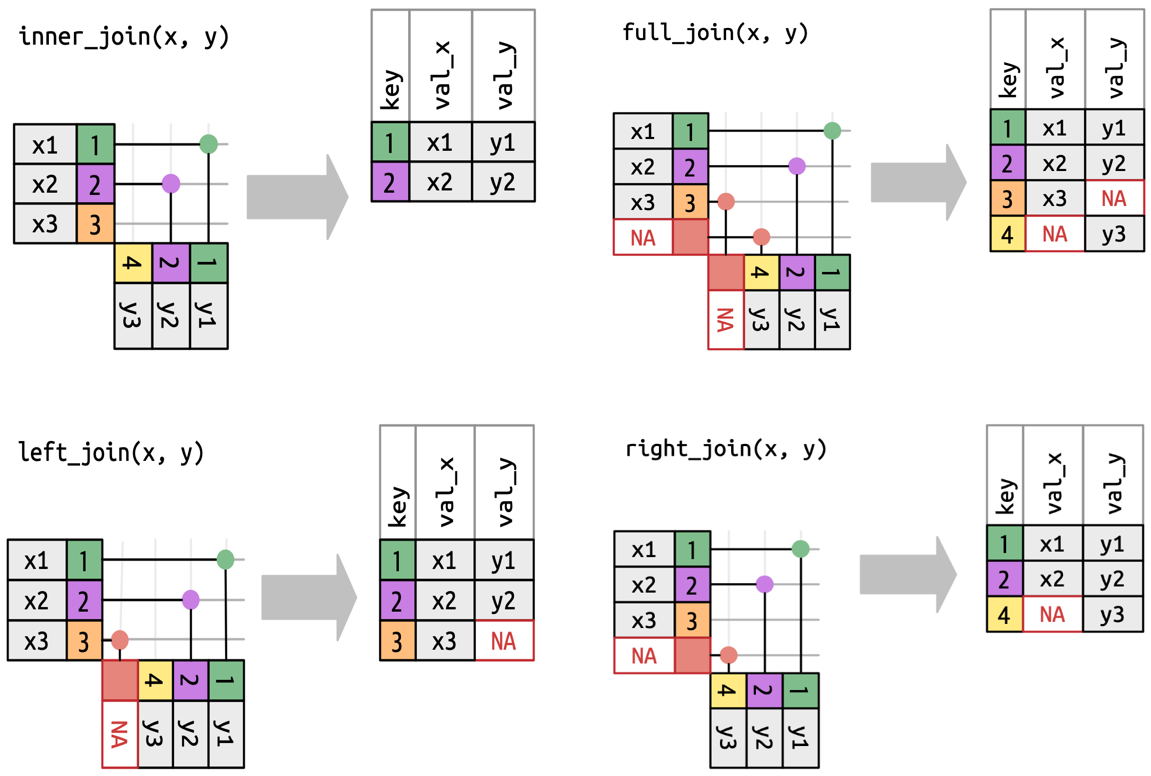
\includegraphics[keepaspectratio]{images/joins.png}}

}

\caption{https://r4ds.hadley.nz/joins}

\end{figure}%

Veri analizi sürecinde, çoğu zaman birden fazla tabloyu \textbf{ortak
bir anahtar} üzerinden birleştirmemiz gerekir.\\
Bu işlem, farklı kaynaklardaki bilgileri \textbf{tek bir veri yapısında
bütünleştirmemizi} sağlar.\\
Örneğin, bir tabloda müşteri bilgileri, diğerinde sipariş bilgileri
olabilir; analiz yapmak için bu tabloları birleştirmemiz gerekir.

R'da veri birleştirme işlemleri hem \textbf{base R fonksiyonları}
(\texttt{merge()}) hem de \textbf{dplyr paketindeki} join fonksiyonları
(\texttt{left\_join()}, \texttt{inner\_join()}, vb.) ile yapılabilir. Bu
bölümde iki yaklaşımı da aynı veri seti üzerinden adım adım
göstereceğiz.

\begin{tcolorbox}[enhanced jigsaw, titlerule=0mm, colbacktitle=quarto-callout-tip-color!10!white, leftrule=.75mm, colback=white, breakable, colframe=quarto-callout-tip-color-frame, bottomtitle=1mm, opacityback=0, left=2mm, title=\textcolor{quarto-callout-tip-color}{\faLightbulb}\hspace{0.5em}{Tip}, rightrule=.15mm, opacitybacktitle=0.6, toptitle=1mm, arc=.35mm, bottomrule=.15mm, toprule=.15mm, coltitle=black]

\textbf{Amaç:}\\
Bu bölümün sonunda, birleştirme türlerini ve hangi durumda hangisinin
kullanılacağını öğreneceksiniz. Ayrıca aynı işlemi hem \texttt{dplyr}
hem de \texttt{base\ R} ile nasıl yapabileceğinizi göreceksiniz.

\end{tcolorbox}

\begin{center}\rule{0.5\linewidth}{0.5pt}\end{center}

\section*{Kullanacağımız Veri
Setleri}\label{kullanacaux11fux131mux131z-veri-setleri}
\addcontentsline{toc}{section}{Kullanacağımız Veri Setleri}

\markright{Kullanacağımız Veri Setleri}

Bu bölümde \texttt{nycflights13} paketindeki veri setlerini
kullanacağız. Bu paket, \textbf{2013 yılı New York uçuş verilerini}
içerir ve ilişkisel yapıdadır. Yani birkaç tablo, ortak anahtarlar
aracılığıyla birbirine bağlanabilir.

\begin{Shaded}
\begin{Highlighting}[]
\FunctionTok{library}\NormalTok{(dplyr)}
\FunctionTok{library}\NormalTok{(nycflights13)}
\end{Highlighting}
\end{Shaded}

\begin{longtable}[]{@{}
  >{\raggedright\arraybackslash}p{(\linewidth - 8\tabcolsep) * \real{0.1304}}
  >{\raggedright\arraybackslash}p{(\linewidth - 8\tabcolsep) * \real{0.2283}}
  >{\raggedright\arraybackslash}p{(\linewidth - 8\tabcolsep) * \real{0.2065}}
  >{\raggedright\arraybackslash}p{(\linewidth - 8\tabcolsep) * \real{0.2174}}
  >{\raggedright\arraybackslash}p{(\linewidth - 8\tabcolsep) * \real{0.2174}}@{}}
\toprule\noalign{}
\begin{minipage}[b]{\linewidth}\raggedright
Tablo
\end{minipage} & \begin{minipage}[b]{\linewidth}\raggedright
İçerik
\end{minipage} & \begin{minipage}[b]{\linewidth}\raggedright
Anahtar Değişken
\end{minipage} & \begin{minipage}[b]{\linewidth}\raggedright
Kayıt Sayısı
\end{minipage} & \begin{minipage}[b]{\linewidth}\raggedright
Sütun Sayısı
\end{minipage} \\
\midrule\noalign{}
\endhead
\bottomrule\noalign{}
\endlastfoot
\texttt{flights} & Uçuş detayları & \texttt{carrier}, \texttt{dest} &
336776 & 19 \\
\texttt{airlines} & Havayolu adları & \texttt{carrier} & 16 & 2 \\
\texttt{airports} & Havaalanı bilgileri & \texttt{faa} & 1458 & 8 \\
\end{longtable}

\begin{Shaded}
\begin{Highlighting}[]
\FunctionTok{glimpse}\NormalTok{(flights)}
\end{Highlighting}
\end{Shaded}

\begin{verbatim}
Rows: 336,776
Columns: 19
$ year           <int> 2013, 2013, 2013, 2013, 2013, 2013, 2013, 2013, 2013, 2~
$ month          <int> 1, 1, 1, 1, 1, 1, 1, 1, 1, 1, 1, 1, 1, 1, 1, 1, 1, 1, 1~
$ day            <int> 1, 1, 1, 1, 1, 1, 1, 1, 1, 1, 1, 1, 1, 1, 1, 1, 1, 1, 1~
$ dep_time       <int> 517, 533, 542, 544, 554, 554, 555, 557, 557, 558, 558, ~
$ sched_dep_time <int> 515, 529, 540, 545, 600, 558, 600, 600, 600, 600, 600, ~
$ dep_delay      <dbl> 2, 4, 2, -1, -6, -4, -5, -3, -3, -2, -2, -2, -2, -2, -1~
$ arr_time       <int> 830, 850, 923, 1004, 812, 740, 913, 709, 838, 753, 849,~
$ sched_arr_time <int> 819, 830, 850, 1022, 837, 728, 854, 723, 846, 745, 851,~
$ arr_delay      <dbl> 11, 20, 33, -18, -25, 12, 19, -14, -8, 8, -2, -3, 7, -1~
$ carrier        <chr> "UA", "UA", "AA", "B6", "DL", "UA", "B6", "EV", "B6", "~
$ flight         <int> 1545, 1714, 1141, 725, 461, 1696, 507, 5708, 79, 301, 4~
$ tailnum        <chr> "N14228", "N24211", "N619AA", "N804JB", "N668DN", "N394~
$ origin         <chr> "EWR", "LGA", "JFK", "JFK", "LGA", "EWR", "EWR", "LGA",~
$ dest           <chr> "IAH", "IAH", "MIA", "BQN", "ATL", "ORD", "FLL", "IAD",~
$ air_time       <dbl> 227, 227, 160, 183, 116, 150, 158, 53, 140, 138, 149, 1~
$ distance       <dbl> 1400, 1416, 1089, 1576, 762, 719, 1065, 229, 944, 733, ~
$ hour           <dbl> 5, 5, 5, 5, 6, 5, 6, 6, 6, 6, 6, 6, 6, 6, 6, 5, 6, 6, 6~
$ minute         <dbl> 15, 29, 40, 45, 0, 58, 0, 0, 0, 0, 0, 0, 0, 0, 0, 59, 0~
$ time_hour      <dttm> 2013-01-01 05:00:00, 2013-01-01 05:00:00, 2013-01-01 0~
\end{verbatim}

\begin{Shaded}
\begin{Highlighting}[]
\FunctionTok{glimpse}\NormalTok{(airlines)}
\end{Highlighting}
\end{Shaded}

\begin{verbatim}
Rows: 16
Columns: 2
$ carrier <chr> "9E", "AA", "AS", "B6", "DL", "EV", "F9", "FL", "HA", "MQ", "O~
$ name    <chr> "Endeavor Air Inc.", "American Airlines Inc.", "Alaska Airline~
\end{verbatim}

\begin{Shaded}
\begin{Highlighting}[]
\FunctionTok{glimpse}\NormalTok{(airports)}
\end{Highlighting}
\end{Shaded}

\begin{verbatim}
Rows: 1,458
Columns: 8
$ faa   <chr> "04G", "06A", "06C", "06N", "09J", "0A9", "0G6", "0G7", "0P2", "~
$ name  <chr> "Lansdowne Airport", "Moton Field Municipal Airport", "Schaumbur~
$ lat   <dbl> 41.13047, 32.46057, 41.98934, 41.43191, 31.07447, 36.37122, 41.4~
$ lon   <dbl> -80.61958, -85.68003, -88.10124, -74.39156, -81.42778, -82.17342~
$ alt   <dbl> 1044, 264, 801, 523, 11, 1593, 730, 492, 1000, 108, 409, 875, 10~
$ tz    <dbl> -5, -6, -6, -5, -5, -5, -5, -5, -5, -8, -5, -6, -5, -5, -5, -5, ~
$ dst   <chr> "A", "A", "A", "A", "A", "A", "A", "A", "U", "A", "A", "U", "A",~
$ tzone <chr> "America/New_York", "America/Chicago", "America/Chicago", "Ameri~
\end{verbatim}

\section*{Anahtar Değişken Nedir?}\label{anahtar-deux11fiux15fken-nedir}
\addcontentsline{toc}{section}{Anahtar Değişken Nedir?}

\markright{Anahtar Değişken Nedir?}

Birleştirme işlemlerinde kullanılan sütunlara \textbf{anahtar değişken}
denir. Bu değişkenler, iki tablo arasında eşleştirmeyi sağlar. Örneğin:

\begin{itemize}
\item
  \texttt{flights} tablosundaki \textbf{\texttt{carrier}},
  \texttt{airlines} tablosundaki \textbf{\texttt{carrier}} ile
  eşleştirilir.
\item
  \texttt{flights} tablosundaki \textbf{\texttt{dest}},
  \texttt{airports} tablosundaki \textbf{\texttt{faa}} ile eşleştirilir.
\end{itemize}

\begin{tcolorbox}[enhanced jigsaw, titlerule=0mm, colbacktitle=quarto-callout-note-color!10!white, leftrule=.75mm, colback=white, breakable, colframe=quarto-callout-note-color-frame, bottomtitle=1mm, opacityback=0, left=2mm, title=\textcolor{quarto-callout-note-color}{\faInfo}\hspace{0.5em}{Note}, rightrule=.15mm, opacitybacktitle=0.6, toptitle=1mm, arc=.35mm, bottomrule=.15mm, toprule=.15mm, coltitle=black]

\textbf{Anahtar Değişken Özellikleri}

\begin{itemize}
\item
  İki tabloda da aynı bilgiyi temsil eder.
\item
  Veri tipleri uyumlu olmalıdır (örneğin, her ikisi de karakter olmalı).
\item
  Tekil veya tekrar eden değerler içerebilir. Tekrarlara göre
  \textbf{ilişki türü (1--1, 1--N, N--M)} belirlenir.
\end{itemize}

\end{tcolorbox}

\section*{Join Kavramı ve Türleri}\label{join-kavramux131-ve-tuxfcrleri}
\addcontentsline{toc}{section}{Join Kavramı ve Türleri}

\markright{Join Kavramı ve Türleri}

\subsection*{Join Nedir?}\label{join-nedir}
\addcontentsline{toc}{subsection}{Join Nedir?}

\textbf{Join}, iki veya daha fazla veri tablosunu ortak bir anahtar
üzerinden birleştirme işlemidir. Sonuçta, tablolar tek bir veri
çerçevesinde birleştirilir. Join türleri, hangi satırların korunacağına
veya eleneceğine göre farklılık gösterir.

\begin{longtable}[]{@{}
  >{\raggedright\arraybackslash}p{(\linewidth - 4\tabcolsep) * \real{0.1359}}
  >{\raggedright\arraybackslash}p{(\linewidth - 4\tabcolsep) * \real{0.6019}}
  >{\raggedright\arraybackslash}p{(\linewidth - 4\tabcolsep) * \real{0.2621}}@{}}
\toprule\noalign{}
\begin{minipage}[b]{\linewidth}\raggedright
Join Türü
\end{minipage} & \begin{minipage}[b]{\linewidth}\raggedright
Tanım
\end{minipage} & \begin{minipage}[b]{\linewidth}\raggedright
Tutulan Satırlar
\end{minipage} \\
\midrule\noalign{}
\endhead
\bottomrule\noalign{}
\endlastfoot
\texttt{left\_join} & Soldaki tüm satırları korur, sağdan eşleşenleri
getirir & Tüm sol tablo \\
\texttt{inner\_join} & Her iki tabloda eşleşen satırları getirir & Ortak
anahtarlar \\
\texttt{right\_join} & Sağdaki tüm satırları korur & Tüm sağ tablo \\
\texttt{full\_join} & Her iki tablodaki tüm satırları birleştirir & Her
iki tablo \\
\texttt{semi\_join} & Sadece sol tablodan, eşleşen satırların alt
kümesini getirir & Sol tablo (eşleşenler) \\
\texttt{anti\_join} & Sol tablodan, eşleşmeyen satırları getirir & Sol
tablo (eşleşmeyenler) \\
\end{longtable}

\subsection*{Kardinalite (İlişki
Türü)}\label{kardinalite-iliux15fki-tuxfcruxfc}
\addcontentsline{toc}{subsection}{Kardinalite (İlişki Türü)}

İki tablo arasındaki ilişki, anahtar değişkenlerin yapısına bağlıdır:

\begin{longtable}[]{@{}
  >{\raggedright\arraybackslash}p{(\linewidth - 4\tabcolsep) * \real{0.2022}}
  >{\raggedright\arraybackslash}p{(\linewidth - 4\tabcolsep) * \real{0.4719}}
  >{\raggedright\arraybackslash}p{(\linewidth - 4\tabcolsep) * \real{0.3258}}@{}}
\toprule\noalign{}
\begin{minipage}[b]{\linewidth}\raggedright
İlişki Türü
\end{minipage} & \begin{minipage}[b]{\linewidth}\raggedright
Tanım
\end{minipage} & \begin{minipage}[b]{\linewidth}\raggedright
Örnek
\end{minipage} \\
\midrule\noalign{}
\endhead
\bottomrule\noalign{}
\endlastfoot
1--1 (bire bir) & Her anahtar her tabloda bir kez geçer & T.C. kimlik
numarası ↔ kişi \\
1--N (bire çok) & Sol tablo tekil, sağ tablo tekrar içerir & Havayolu ↔
Uçuşlar \\
N--M (çoktan çok) & Her iki tabloda da tekrarlar vardır & Öğrenci ↔
Ders \\
\end{longtable}

Bu durum, birleştirme sonrası satır sayısını doğrudan etkiler. Örneğin
1--N ilişkisinde satır sayısı artabilir.

\subsection*{R'de Join
Yaklaşımları}\label{rde-join-yaklaux15fux131mlarux131}
\addcontentsline{toc}{subsection}{R'de Join Yaklaşımları}

R dilinde iki temel yaklaşım vardır:

\begin{longtable}[]{@{}
  >{\raggedright\arraybackslash}p{(\linewidth - 4\tabcolsep) * \real{0.0982}}
  >{\raggedright\arraybackslash}p{(\linewidth - 4\tabcolsep) * \real{0.8214}}
  >{\raggedright\arraybackslash}p{(\linewidth - 4\tabcolsep) * \real{0.0804}}@{}}
\toprule\noalign{}
\begin{minipage}[b]{\linewidth}\raggedright
Yaklaşım
\end{minipage} & \begin{minipage}[b]{\linewidth}\raggedright
Fonksiyon
\end{minipage} & \begin{minipage}[b]{\linewidth}\raggedright
Paket
\end{minipage} \\
\midrule\noalign{}
\endhead
\bottomrule\noalign{}
\endlastfoot
Base R & \texttt{merge()} & Temel R \\
Tidyverse & \texttt{left\_join()}, \texttt{inner\_join()},
\texttt{right\_join()}, \texttt{full\_join()}, \texttt{semi\_join()},
\texttt{anti\_join()} & \texttt{dplyr} \\
\end{longtable}

\begin{tcolorbox}[enhanced jigsaw, titlerule=0mm, colbacktitle=quarto-callout-note-color!10!white, leftrule=.75mm, colback=white, breakable, colframe=quarto-callout-note-color-frame, bottomtitle=1mm, opacityback=0, left=2mm, title=\textcolor{quarto-callout-note-color}{\faInfo}\hspace{0.5em}{Note}, rightrule=.15mm, opacitybacktitle=0.6, toptitle=1mm, arc=.35mm, bottomrule=.15mm, toprule=.15mm, coltitle=black]

\texttt{dplyr} fonksiyonları daha \textbf{okunabilir}, \textbf{tutarlı},
ve \textbf{pipe (\%\textgreater\%)} yapısı ile çalışmaya uygundur.\\
Ancak \texttt{merge()} hâlâ birçok eski kodda ve küçük projelerde yaygın
biçimde kullanılır.\\
Bu yüzden bu bölümde her iki yöntemi de göreceğiz.

\end{tcolorbox}

\section*{Left Join}\label{left-join}
\addcontentsline{toc}{section}{Left Join}

\markright{Left Join}

\texttt{left\_join()} veya \texttt{merge(...,\ all.x\ =\ TRUE)}
işlemleri, \textbf{soldaki tablodaki tüm satırları} koruyup, sağdaki
tablodan yalnızca eşleşen kayıtları ekler. Bu en sık kullanılan
birleştirme türüdür; çünkü genellikle ``asıl veri setini'' korumak
isteriz.

\textbf{Amaç:} Her uçuşun \texttt{carrier} bilgisine karşılık gelen
\textbf{havayolu adını} ekleyelim. Yani \texttt{flights} tablosundaki
\texttt{carrier} değişkenini, \texttt{airlines} tablosundaki
\texttt{carrier} ile eşleştireceğiz.

\textbf{Beklenti}

\begin{itemize}
\tightlist
\item
  Satır sayısı \textbf{flights ile aynı} kalmalı.
\item
  Eşleşmeyen \texttt{carrier} değerleri varsa \texttt{NA} gözükecek.
\item
  Sonuçta yeni sütun: \texttt{name} (= havayolu adı).
\end{itemize}

\begin{center}\rule{0.5\linewidth}{0.5pt}\end{center}

\begin{Shaded}
\begin{Highlighting}[]
\NormalTok{fl\_joined }\OtherTok{\textless{}{-}}\NormalTok{ flights }\SpecialCharTok{\%\textgreater{}\%}
  \FunctionTok{left\_join}\NormalTok{(airlines, }\AttributeTok{by =} \StringTok{"carrier"}\NormalTok{)}

\CommentTok{\# Satır sayısı değişti mi?}
\FunctionTok{tibble}\NormalTok{(}
  \AttributeTok{onceki =} \FunctionTok{nrow}\NormalTok{(flights),}
  \AttributeTok{sonraki =} \FunctionTok{nrow}\NormalTok{(fl\_joined)}
\NormalTok{)}
\end{Highlighting}
\end{Shaded}

\begin{verbatim}
# A tibble: 1 x 2
  onceki sonraki
   <int>   <int>
1 336776  336776
\end{verbatim}

Sonuç değişmedi: \texttt{left\_join()} soldaki tabloyu (flights) esas
alır.

Yeni değişkenleri görelim:

\begin{Shaded}
\begin{Highlighting}[]
\NormalTok{fl\_joined }\SpecialCharTok{\%\textgreater{}\%}
\FunctionTok{select}\NormalTok{(year, month, day, carrier, name) }\SpecialCharTok{\%\textgreater{}\%}
\FunctionTok{distinct}\NormalTok{(carrier, name) }\SpecialCharTok{\%\textgreater{}\%}
\FunctionTok{arrange}\NormalTok{(carrier) }\SpecialCharTok{\%\textgreater{}\%}
\FunctionTok{head}\NormalTok{(}\DecValTok{10}\NormalTok{)}
\end{Highlighting}
\end{Shaded}

\begin{verbatim}
# A tibble: 10 x 2
   carrier name                       
   <chr>   <chr>                      
 1 9E      Endeavor Air Inc.          
 2 AA      American Airlines Inc.     
 3 AS      Alaska Airlines Inc.       
 4 B6      JetBlue Airways            
 5 DL      Delta Air Lines Inc.       
 6 EV      ExpressJet Airlines Inc.   
 7 F9      Frontier Airlines Inc.     
 8 FL      AirTran Airways Corporation
 9 HA      Hawaiian Airlines Inc.     
10 MQ      Envoy Air                  
\end{verbatim}

\begin{tcolorbox}[enhanced jigsaw, titlerule=0mm, colbacktitle=quarto-callout-note-color!10!white, leftrule=.75mm, colback=white, breakable, colframe=quarto-callout-note-color-frame, bottomtitle=1mm, opacityback=0, left=2mm, title=\textcolor{quarto-callout-note-color}{\faInfo}\hspace{0.5em}{Note}, rightrule=.15mm, opacitybacktitle=0.6, toptitle=1mm, arc=.35mm, bottomrule=.15mm, toprule=.15mm, coltitle=black]

Burada \texttt{name} sütunu \texttt{airlines} tablosundan geldi.\\
Eğer iki tabloda aynı isimli başka sütunlar olsaydı, \texttt{dplyr}
otomatik olarak \texttt{.x} ve \texttt{.y} sonekleri eklerdi.

\end{tcolorbox}

\textbf{Base R ile Aynı İşlem}

Base R'de aynı işlem \texttt{merge()} ile yapılır.
\texttt{all.x\ =\ TRUE} parametresi, soldan birleştirme anlamına gelir.

\begin{Shaded}
\begin{Highlighting}[]
\NormalTok{fl\_joined\_base }\OtherTok{\textless{}{-}} \FunctionTok{merge}\NormalTok{(}
\NormalTok{flights,}
\NormalTok{airlines,}
\AttributeTok{by =} \StringTok{"carrier"}\NormalTok{,}
\AttributeTok{all.x =} \ConstantTok{TRUE}
\NormalTok{)}

\CommentTok{\# Satır sayısı kontrolü}

\FunctionTok{c}\NormalTok{(}\AttributeTok{before =} \FunctionTok{nrow}\NormalTok{(flights), }\AttributeTok{after =} \FunctionTok{nrow}\NormalTok{(fl\_joined\_base))}
\end{Highlighting}
\end{Shaded}

\begin{verbatim}
before  after 
336776 336776 
\end{verbatim}

\begin{Shaded}
\begin{Highlighting}[]
\FunctionTok{head}\NormalTok{(fl\_joined\_base[}\FunctionTok{c}\NormalTok{(}\StringTok{"carrier"}\NormalTok{, }\StringTok{"name"}\NormalTok{)], }\DecValTok{10}\NormalTok{)}
\end{Highlighting}
\end{Shaded}

\begin{verbatim}
   carrier              name
1       9E Endeavor Air Inc.
2       9E Endeavor Air Inc.
3       9E Endeavor Air Inc.
4       9E Endeavor Air Inc.
5       9E Endeavor Air Inc.
6       9E Endeavor Air Inc.
7       9E Endeavor Air Inc.
8       9E Endeavor Air Inc.
9       9E Endeavor Air Inc.
10      9E Endeavor Air Inc.
\end{verbatim}

\begin{longtable}[]{@{}
  >{\raggedright\arraybackslash}p{(\linewidth - 4\tabcolsep) * \real{0.1261}}
  >{\raggedright\arraybackslash}p{(\linewidth - 4\tabcolsep) * \real{0.2941}}
  >{\raggedright\arraybackslash}p{(\linewidth - 4\tabcolsep) * \real{0.5798}}@{}}
\toprule\noalign{}
\begin{minipage}[b]{\linewidth}\raggedright
Özellik
\end{minipage} & \begin{minipage}[b]{\linewidth}\raggedright
\texttt{dplyr::left\_join()}
\end{minipage} & \begin{minipage}[b]{\linewidth}\raggedright
\texttt{base::merge()}
\end{minipage} \\
\midrule\noalign{}
\endhead
\bottomrule\noalign{}
\endlastfoot
Sözdizimi & Daha okunaklı (\texttt{by\ =\ "carrier"}) & Uzun, parametre
odaklı \\
Varsayılan & Sadece belirttiğin \texttt{by} üzerinden & Eğer \texttt{by}
yoksa, ortak isimleri bulup otomatik join yapar (dikkat!) \\
Sonekler & \texttt{.x} ve \texttt{.y} & \texttt{.x} ve \texttt{.y} veya
\texttt{.1} ve \texttt{.2} \\
Performans & Genelde daha hızlı & Büyük veride yavaş olabilir \\
Okunabilirlik & 👍 & 🟡 \\
\end{longtable}

\subsection*{Küçük Deneme: Eşleşmeyen Anahtar
Durumu}\label{kuxfcuxe7uxfck-deneme-eux15fleux15fmeyen-anahtar-durumu}
\addcontentsline{toc}{subsection}{Küçük Deneme: Eşleşmeyen Anahtar
Durumu}

Varsayalım \texttt{airlines} tablosundan bir satırı çıkaralım ve join
yapalım; ne olur?

\begin{Shaded}
\begin{Highlighting}[]
\NormalTok{airlines\_miss }\OtherTok{\textless{}{-}}\NormalTok{ airlines }\SpecialCharTok{\%\textgreater{}\%} \FunctionTok{filter}\NormalTok{(carrier }\SpecialCharTok{!=} \StringTok{"UA"}\NormalTok{)}
\NormalTok{fl\_test }\OtherTok{\textless{}{-}}\NormalTok{ flights }\SpecialCharTok{\%\textgreater{}\%} \FunctionTok{left\_join}\NormalTok{(airlines\_miss, }\AttributeTok{by =} \StringTok{"carrier"}\NormalTok{)}

\NormalTok{fl\_test }\SpecialCharTok{\%\textgreater{}\%}
\FunctionTok{filter}\NormalTok{(}\FunctionTok{is.na}\NormalTok{(name)) }\SpecialCharTok{\%\textgreater{}\%}
\FunctionTok{distinct}\NormalTok{(carrier) }\SpecialCharTok{\%\textgreater{}\%}
\FunctionTok{head}\NormalTok{()}
\end{Highlighting}
\end{Shaded}

\begin{verbatim}
# A tibble: 1 x 1
  carrier
  <chr>  
1 UA     
\end{verbatim}

Sonuçta \texttt{name\ =\ NA} olan satırlar, \texttt{airlines} tablosunda
karşılığı olmayan taşıyıcılardır.

\begin{tcolorbox}[enhanced jigsaw, titlerule=0mm, colbacktitle=quarto-callout-note-color!10!white, leftrule=.75mm, colback=white, breakable, colframe=quarto-callout-note-color-frame, bottomtitle=1mm, opacityback=0, left=2mm, title=\textcolor{quarto-callout-note-color}{\faInfo}\hspace{0.5em}{Note}, rightrule=.15mm, opacitybacktitle=0.6, toptitle=1mm, arc=.35mm, bottomrule=.15mm, toprule=.15mm, coltitle=black]

Bu tip satırlar \textbf{veri tutarlılığı} açısından önemlidir.\\
Gerçek analizlerde bu tür durumlar genellikle hatalı veya eksik kod
anlamına gelir.

\end{tcolorbox}

\section*{Kısa Özet}\label{kux131sa-uxf6zet}
\addcontentsline{toc}{section}{Kısa Özet}

\markright{Kısa Özet}

\begin{itemize}
\item
  \texttt{left\_join()}: soldaki tüm satırları korur.
\item
  \texttt{merge(...,\ all.x\ =\ TRUE)}: aynı işlevi base R'de yapar.
\item
  Eşleşmeyen kayıtlar → \texttt{NA}.
\item
  Kontrol: satır sayısı değişmemeli.
\item
  Kod tabloları eklemek için en güvenli yöntemdir.
\end{itemize}

\section*{Inner Join}\label{inner-join}
\addcontentsline{toc}{section}{Inner Join}

\markright{Inner Join}

\texttt{inner\_join()} veya \texttt{merge(...,\ all\ =\ FALSE)}
işlemleri, iki tablodaki \textbf{ortak anahtar değerlerine sahip}
satırları getirir. Yani her iki tabloda da eşleşen kayıtlar kalır;
eşleşmeyenler atılır.

\textbf{Amaç:} Yalnızca hem \texttt{flights} hem de \texttt{airlines}
tablolarında \textbf{karşılığı olan havayolu kodlarını} içeren satırları
tutmak.

\textbf{Beklenti}

\begin{itemize}
\tightlist
\item
  Satır sayısı \texttt{flights}'tan \textbf{daha az} olabilir.
\item
  Her iki tablodan da \texttt{carrier} eşleşmeyenler çıkarılır.
\item
  \texttt{NA} değer \textbf{olmamalıdır} çünkü sadece eşleşenler alınır.
\end{itemize}

\begin{center}\rule{0.5\linewidth}{0.5pt}\end{center}

\textbf{dplyr ile Inner Join}

\begin{Shaded}
\begin{Highlighting}[]
\NormalTok{fl\_inner }\OtherTok{\textless{}{-}}\NormalTok{ flights }\SpecialCharTok{\%\textgreater{}\%}
  \FunctionTok{inner\_join}\NormalTok{(airlines, }\AttributeTok{by =} \StringTok{"carrier"}\NormalTok{)}

\FunctionTok{tibble}\NormalTok{(}
  \AttributeTok{flights\_satir =} \FunctionTok{nrow}\NormalTok{(flights),}
  \AttributeTok{inner\_join\_satir =} \FunctionTok{nrow}\NormalTok{(fl\_inner)}
\NormalTok{)}
\end{Highlighting}
\end{Shaded}

\begin{verbatim}
# A tibble: 1 x 2
  flights_satir inner_join_satir
          <int>            <int>
1        336776           336776
\end{verbatim}

Görüldüğü gibi satır sayısı azaldıysa, bazı \texttt{carrier} değerleri
yalnızca bir tabloda var demektir. Sonuçtan küçük bir örnek:

\begin{Shaded}
\begin{Highlighting}[]
\NormalTok{fl\_inner }\SpecialCharTok{\%\textgreater{}\%}
\FunctionTok{select}\NormalTok{(year, month, day, carrier, name) }\SpecialCharTok{\%\textgreater{}\%}
\FunctionTok{distinct}\NormalTok{(carrier, name) }\SpecialCharTok{\%\textgreater{}\%}
\FunctionTok{arrange}\NormalTok{(carrier) }\SpecialCharTok{\%\textgreater{}\%}
\FunctionTok{head}\NormalTok{(}\DecValTok{10}\NormalTok{)}
\end{Highlighting}
\end{Shaded}

\begin{verbatim}
# A tibble: 10 x 2
   carrier name                       
   <chr>   <chr>                      
 1 9E      Endeavor Air Inc.          
 2 AA      American Airlines Inc.     
 3 AS      Alaska Airlines Inc.       
 4 B6      JetBlue Airways            
 5 DL      Delta Air Lines Inc.       
 6 EV      ExpressJet Airlines Inc.   
 7 F9      Frontier Airlines Inc.     
 8 FL      AirTran Airways Corporation
 9 HA      Hawaiian Airlines Inc.     
10 MQ      Envoy Air                  
\end{verbatim}

\begin{tcolorbox}[enhanced jigsaw, titlerule=0mm, colbacktitle=quarto-callout-tip-color!10!white, leftrule=.75mm, colback=white, breakable, colframe=quarto-callout-tip-color-frame, bottomtitle=1mm, opacityback=0, left=2mm, title=\textcolor{quarto-callout-tip-color}{\faLightbulb}\hspace{0.5em}{Tip}, rightrule=.15mm, opacitybacktitle=0.6, toptitle=1mm, arc=.35mm, bottomrule=.15mm, toprule=.15mm, coltitle=black]

\texttt{inner\_join()} genellikle \textbf{veri kesişimlerini} bulmak
için kullanılır. Örneğin, yalnızca hem satış listesinde hem stok
listesinde bulunan ürünleri görmek istediğinizde.

\end{tcolorbox}

\textbf{Base R ile Inner Join}

Aynı mantık \texttt{merge()} fonksiyonunda varsayılan olarak geçerlidir.
Yani \texttt{all\ =\ FALSE} (veya hiç yazmazsanız) \textbf{inner join}
anlamına gelir.

\begin{Shaded}
\begin{Highlighting}[]
\NormalTok{fl\_inner\_base }\OtherTok{\textless{}{-}} \FunctionTok{merge}\NormalTok{(}
\NormalTok{flights,}
\NormalTok{airlines,}
\AttributeTok{by =} \StringTok{"carrier"}\NormalTok{,}
\AttributeTok{all =} \ConstantTok{FALSE}
\NormalTok{)}

\FunctionTok{c}\NormalTok{(}\AttributeTok{before =} \FunctionTok{nrow}\NormalTok{(flights), }\AttributeTok{after =} \FunctionTok{nrow}\NormalTok{(fl\_inner\_base))}
\end{Highlighting}
\end{Shaded}

\begin{verbatim}
before  after 
336776 336776 
\end{verbatim}

\begin{Shaded}
\begin{Highlighting}[]
\FunctionTok{head}\NormalTok{(fl\_inner\_base[}\FunctionTok{c}\NormalTok{(}\StringTok{"carrier"}\NormalTok{, }\StringTok{"name"}\NormalTok{)], }\DecValTok{10}\NormalTok{)}
\end{Highlighting}
\end{Shaded}

\begin{verbatim}
   carrier              name
1       9E Endeavor Air Inc.
2       9E Endeavor Air Inc.
3       9E Endeavor Air Inc.
4       9E Endeavor Air Inc.
5       9E Endeavor Air Inc.
6       9E Endeavor Air Inc.
7       9E Endeavor Air Inc.
8       9E Endeavor Air Inc.
9       9E Endeavor Air Inc.
10      9E Endeavor Air Inc.
\end{verbatim}

\begin{longtable}[]{@{}
  >{\raggedright\arraybackslash}p{(\linewidth - 4\tabcolsep) * \real{0.2530}}
  >{\raggedright\arraybackslash}p{(\linewidth - 4\tabcolsep) * \real{0.3735}}
  >{\raggedright\arraybackslash}p{(\linewidth - 4\tabcolsep) * \real{0.3735}}@{}}
\toprule\noalign{}
\begin{minipage}[b]{\linewidth}\raggedright
Özellik
\end{minipage} & \begin{minipage}[b]{\linewidth}\raggedright
\texttt{dplyr::inner\_join()}
\end{minipage} & \begin{minipage}[b]{\linewidth}\raggedright
\texttt{base::merge()}
\end{minipage} \\
\midrule\noalign{}
\endhead
\bottomrule\noalign{}
\endlastfoot
Varsayılan davranış & Yalnızca eşleşenleri tutar & Aynı \\
Satır sayısı & Azalabilir & Azalabilir \\
\texttt{NA} değerler & Oluşmaz & Oluşmaz \\
Kullanım alanı & Eşleşen kayıtları filtrelemek & Eşleşen kayıtları
filtrelemek \\
\end{longtable}

\begin{tcolorbox}[enhanced jigsaw, titlerule=0mm, colbacktitle=quarto-callout-note-color!10!white, leftrule=.75mm, colback=white, breakable, colframe=quarto-callout-note-color-frame, bottomtitle=1mm, opacityback=0, left=2mm, title=\textcolor{quarto-callout-note-color}{\faInfo}\hspace{0.5em}{Note}, rightrule=.15mm, opacitybacktitle=0.6, toptitle=1mm, arc=.35mm, bottomrule=.15mm, toprule=.15mm, coltitle=black]

\textbf{Kısa Hatırlatma:}\\

\texttt{inner\_join()} sadece \textbf{ortak anahtarları} getirir. Bir
tabloda olup diğerinde olmayan kayıtlar \textbf{tamamen dışlanır}. Bu
nedenle veri kaybı olmaması istenen durumlarda \texttt{left\_join()}
tercih edilmelidir.

\end{tcolorbox}

\section*{Right Join ve Full Join}\label{right-join-ve-full-join}
\addcontentsline{toc}{section}{Right Join ve Full Join}

\markright{Right Join ve Full Join}

Bu iki join türü, kapsayıcı birleştirmeler olarak adlandırılır.\\
Amaç, iki tablodaki \textbf{tüm bilgileri korumaktır} --- ancak
satırların hangi taraftan korunduğu değişir.

\subsection*{Right Join}\label{right-join}
\addcontentsline{toc}{subsection}{Right Join}

\texttt{right\_join()} veya \texttt{merge(...,\ all.y\ =\ TRUE)}
işlemleri, \textbf{sağdaki tablonun tüm satırlarını} korur.\\
Soldaki tablodan yalnızca eşleşen kayıtlar getirilir.

\textbf{Amaç:} Tüm \texttt{airlines} kayıtlarını koruyalım, fakat
\texttt{flights} tablosundan sadece eşleşenleri alalım. Bu, ``sağ tarafı
referans alan'' bir birleştirmedir.

\begin{center}\rule{0.5\linewidth}{0.5pt}\end{center}

\textbf{dplyr ile Right Join}

\begin{Shaded}
\begin{Highlighting}[]
\NormalTok{fl\_right }\OtherTok{\textless{}{-}}\NormalTok{ flights }\SpecialCharTok{\%\textgreater{}\%}
  \FunctionTok{right\_join}\NormalTok{(airlines, }\AttributeTok{by =} \StringTok{"carrier"}\NormalTok{)}

\FunctionTok{tibble}\NormalTok{(}
  \AttributeTok{flights\_satir =} \FunctionTok{nrow}\NormalTok{(flights),}
  \AttributeTok{airlines\_satir =} \FunctionTok{nrow}\NormalTok{(airlines),}
  \AttributeTok{right\_join\_satir =} \FunctionTok{nrow}\NormalTok{(fl\_right)}
\NormalTok{)}
\end{Highlighting}
\end{Shaded}

\begin{verbatim}
# A tibble: 1 x 3
  flights_satir airlines_satir right_join_satir
          <int>          <int>            <int>
1        336776             16           336776
\end{verbatim}

\begin{Shaded}
\begin{Highlighting}[]
\NormalTok{fl\_right }\SpecialCharTok{\%\textgreater{}\%}
\FunctionTok{select}\NormalTok{(carrier, name) }\SpecialCharTok{\%\textgreater{}\%}
\FunctionTok{distinct}\NormalTok{(carrier, name)}
\end{Highlighting}
\end{Shaded}

\begin{verbatim}
# A tibble: 16 x 2
   carrier name                       
   <chr>   <chr>                      
 1 UA      United Air Lines Inc.      
 2 AA      American Airlines Inc.     
 3 B6      JetBlue Airways            
 4 DL      Delta Air Lines Inc.       
 5 EV      ExpressJet Airlines Inc.   
 6 MQ      Envoy Air                  
 7 US      US Airways Inc.            
 8 WN      Southwest Airlines Co.     
 9 VX      Virgin America             
10 FL      AirTran Airways Corporation
11 AS      Alaska Airlines Inc.       
12 9E      Endeavor Air Inc.          
13 F9      Frontier Airlines Inc.     
14 HA      Hawaiian Airlines Inc.     
15 YV      Mesa Airlines Inc.         
16 OO      SkyWest Airlines Inc.      
\end{verbatim}

\begin{tcolorbox}[enhanced jigsaw, titlerule=0mm, colbacktitle=quarto-callout-note-color!10!white, leftrule=.75mm, colback=white, breakable, colframe=quarto-callout-note-color-frame, bottomtitle=1mm, opacityback=0, left=2mm, title=\textcolor{quarto-callout-note-color}{\faInfo}\hspace{0.5em}{Note}, rightrule=.15mm, opacitybacktitle=0.6, toptitle=1mm, arc=.35mm, bottomrule=.15mm, toprule=.15mm, coltitle=black]

\texttt{right\_join()} işlemi özellikle ``kod tablosu'' tarafındaki tüm
değerlerin korunmasını istediğimiz durumlarda kullanılır.\\
Örneğin: tüm müşteri listesi sağda, yalnızca satış yapanlar soldaysa.

\end{tcolorbox}

\textbf{Base R ile Right Join}

Base R'de aynı işlem \texttt{merge(...,\ all.y\ =\ TRUE)} parametresiyle
yapılır.

\begin{Shaded}
\begin{Highlighting}[]
\NormalTok{fl\_right\_base }\OtherTok{\textless{}{-}} \FunctionTok{merge}\NormalTok{(}
\NormalTok{flights,}
\NormalTok{airlines,}
\AttributeTok{by =} \StringTok{"carrier"}\NormalTok{,}
\AttributeTok{all.y =} \ConstantTok{TRUE}
\NormalTok{)}

\FunctionTok{c}\NormalTok{(}\AttributeTok{before =} \FunctionTok{nrow}\NormalTok{(airlines), }\AttributeTok{after =} \FunctionTok{nrow}\NormalTok{(fl\_right\_base))}
\end{Highlighting}
\end{Shaded}

\begin{verbatim}
before  after 
    16 336776 
\end{verbatim}

\begin{Shaded}
\begin{Highlighting}[]
\FunctionTok{head}\NormalTok{(fl\_right\_base[}\FunctionTok{c}\NormalTok{(}\StringTok{"carrier"}\NormalTok{, }\StringTok{"name"}\NormalTok{)], }\DecValTok{10}\NormalTok{)}
\end{Highlighting}
\end{Shaded}

\begin{verbatim}
   carrier              name
1       9E Endeavor Air Inc.
2       9E Endeavor Air Inc.
3       9E Endeavor Air Inc.
4       9E Endeavor Air Inc.
5       9E Endeavor Air Inc.
6       9E Endeavor Air Inc.
7       9E Endeavor Air Inc.
8       9E Endeavor Air Inc.
9       9E Endeavor Air Inc.
10      9E Endeavor Air Inc.
\end{verbatim}

\subsection*{Full Join}\label{full-join}
\addcontentsline{toc}{subsection}{Full Join}

\texttt{full\_join()} veya \texttt{merge(...,\ all\ =\ TRUE)} işlemleri,
\textbf{her iki tablodaki tüm anahtar değerlerini} birleştirir.\\
Eşleşmeyen satırların bulunduğu taraflarda \texttt{NA} değerler oluşur.

\textbf{Amaç:} \texttt{flights} ve \texttt{airlines} tablolarını tüm
anahtarlarla birleştirelim. Böylece her iki tarafta olup diğerinde
olmayan kayıtlar da görünür.

\textbf{dplyr ile Full Join}

\begin{Shaded}
\begin{Highlighting}[]
\NormalTok{fl\_full }\OtherTok{\textless{}{-}}\NormalTok{ flights }\SpecialCharTok{\%\textgreater{}\%}
\FunctionTok{full\_join}\NormalTok{(airlines, }\AttributeTok{by =} \StringTok{"carrier"}\NormalTok{)}

\FunctionTok{tibble}\NormalTok{(}
\AttributeTok{flights\_satir =} \FunctionTok{nrow}\NormalTok{(flights),}
\AttributeTok{airlines\_satir =} \FunctionTok{nrow}\NormalTok{(airlines),}
\AttributeTok{full\_join\_satir =} \FunctionTok{nrow}\NormalTok{(fl\_full)}
\NormalTok{)}
\end{Highlighting}
\end{Shaded}

\begin{verbatim}
# A tibble: 1 x 3
  flights_satir airlines_satir full_join_satir
          <int>          <int>           <int>
1        336776             16          336776
\end{verbatim}

\begin{Shaded}
\begin{Highlighting}[]
\NormalTok{fl\_full }\SpecialCharTok{\%\textgreater{}\%}
\FunctionTok{select}\NormalTok{(carrier, name) }\SpecialCharTok{\%\textgreater{}\%}
\FunctionTok{distinct}\NormalTok{(carrier, name) }\SpecialCharTok{\%\textgreater{}\%}
\FunctionTok{arrange}\NormalTok{(carrier) }\SpecialCharTok{\%\textgreater{}\%}
\FunctionTok{head}\NormalTok{(}\DecValTok{10}\NormalTok{)}
\end{Highlighting}
\end{Shaded}

\begin{verbatim}
# A tibble: 10 x 2
   carrier name                       
   <chr>   <chr>                      
 1 9E      Endeavor Air Inc.          
 2 AA      American Airlines Inc.     
 3 AS      Alaska Airlines Inc.       
 4 B6      JetBlue Airways            
 5 DL      Delta Air Lines Inc.       
 6 EV      ExpressJet Airlines Inc.   
 7 F9      Frontier Airlines Inc.     
 8 FL      AirTran Airways Corporation
 9 HA      Hawaiian Airlines Inc.     
10 MQ      Envoy Air                  
\end{verbatim}

\textbf{Base R ile Full Join}

Base R'de \texttt{all\ =\ TRUE} kullanıldığında \textbf{full join} elde
edilir:

\begin{Shaded}
\begin{Highlighting}[]
\NormalTok{fl\_full\_base }\OtherTok{\textless{}{-}} \FunctionTok{merge}\NormalTok{(}
\NormalTok{flights,}
\NormalTok{airlines,}
\AttributeTok{by =} \StringTok{"carrier"}\NormalTok{,}
\AttributeTok{all =} \ConstantTok{TRUE}
\NormalTok{)}

\FunctionTok{c}\NormalTok{(}\AttributeTok{before =} \FunctionTok{nrow}\NormalTok{(flights) }\SpecialCharTok{+} \FunctionTok{nrow}\NormalTok{(airlines), }\AttributeTok{after =} \FunctionTok{nrow}\NormalTok{(fl\_full\_base))}
\end{Highlighting}
\end{Shaded}

\begin{verbatim}
before  after 
336792 336776 
\end{verbatim}

\begin{Shaded}
\begin{Highlighting}[]
\FunctionTok{head}\NormalTok{(fl\_full\_base[}\FunctionTok{c}\NormalTok{(}\StringTok{"carrier"}\NormalTok{, }\StringTok{"name"}\NormalTok{)], }\DecValTok{10}\NormalTok{)}
\end{Highlighting}
\end{Shaded}

\begin{verbatim}
   carrier              name
1       9E Endeavor Air Inc.
2       9E Endeavor Air Inc.
3       9E Endeavor Air Inc.
4       9E Endeavor Air Inc.
5       9E Endeavor Air Inc.
6       9E Endeavor Air Inc.
7       9E Endeavor Air Inc.
8       9E Endeavor Air Inc.
9       9E Endeavor Air Inc.
10      9E Endeavor Air Inc.
\end{verbatim}

\section*{Özet}\label{uxf6zet}
\addcontentsline{toc}{section}{Özet}

\markright{Özet}

\begin{longtable}[]{@{}
  >{\raggedright\arraybackslash}p{(\linewidth - 8\tabcolsep) * \real{0.1121}}
  >{\raggedright\arraybackslash}p{(\linewidth - 8\tabcolsep) * \real{0.1682}}
  >{\raggedright\arraybackslash}p{(\linewidth - 8\tabcolsep) * \real{0.2617}}
  >{\raggedright\arraybackslash}p{(\linewidth - 8\tabcolsep) * \real{0.1402}}
  >{\raggedright\arraybackslash}p{(\linewidth - 8\tabcolsep) * \real{0.3178}}@{}}
\toprule\noalign{}
\begin{minipage}[b]{\linewidth}\raggedright
Join Türü
\end{minipage} & \begin{minipage}[b]{\linewidth}\raggedright
dplyr Fonksiyonu
\end{minipage} & \begin{minipage}[b]{\linewidth}\raggedright
Base R Eşdeğeri
\end{minipage} & \begin{minipage}[b]{\linewidth}\raggedright
Korunan Taraf
\end{minipage} & \begin{minipage}[b]{\linewidth}\raggedright
Eşleşmeyenler
\end{minipage} \\
\midrule\noalign{}
\endhead
\bottomrule\noalign{}
\endlastfoot
Left Join & \texttt{left\_join()} & \texttt{merge(...,\ all.x\ =\ TRUE)}
& Sol tablo & Sağ taraf \texttt{NA} \\
Right Join & \texttt{right\_join()} &
\texttt{merge(...,\ all.y\ =\ TRUE)} & Sağ tablo & Sol taraf
\texttt{NA} \\
Full Join & \texttt{full\_join()} & \texttt{merge(...,\ all\ =\ TRUE)} &
Her iki tablo & Her iki tarafta da \texttt{NA} olabilir \\
\end{longtable}

\begin{tcolorbox}[enhanced jigsaw, titlerule=0mm, colbacktitle=quarto-callout-note-color!10!white, leftrule=.75mm, colback=white, breakable, colframe=quarto-callout-note-color-frame, bottomtitle=1mm, opacityback=0, left=2mm, title=\textcolor{quarto-callout-note-color}{\faInfo}\hspace{0.5em}{Note}, rightrule=.15mm, opacitybacktitle=0.6, toptitle=1mm, arc=.35mm, bottomrule=.15mm, toprule=.15mm, coltitle=black]

\texttt{full\_join()} verilerin iki farklı kaynaktan geldiği ve
\textbf{birleştirmenin tamlığı} kontrol edilmek istendiği durumlarda
kullanışlıdır. Örneğin: iki dönem verisini, iki kurum listesini veya iki
sürümü birleştirirken.

\end{tcolorbox}

\section*{Filtreleme Türü Join'ler (Semi Join ve Anti
Join)}\label{filtreleme-tuxfcruxfc-joinler-semi-join-ve-anti-join}
\addcontentsline{toc}{section}{Filtreleme Türü Join'ler (Semi Join ve
Anti Join)}

\markright{Filtreleme Türü Join'ler (Semi Join ve Anti Join)}

Bu iki join türü, tablo yapısını değiştirmez; yalnızca \textbf{satır
seçimi (filtreleme)} yapar. Yani \texttt{semi\_join()} ve
\texttt{anti\_join()} yeni sütunlar eklemez, sadece \textbf{sol
tablodan} bazı satırları seçer. Bu işlemler SQL'de sırasıyla \emph{WHERE
EXISTS} ve \emph{WHERE NOT EXISTS} karşılığına denktir.

\subsection*{semi\_join()}\label{semi_join}
\addcontentsline{toc}{subsection}{semi\_join()}

\texttt{semi\_join()} sol tablodaki satırlardan, sağ tablodaki
anahtarlarla \textbf{eşleşenleri} tutar. Eşleşmeyen satırlar atılır.
Yeni sütun eklenmez, sadece satır sayısı azalabilir.

\textbf{Amaç:} \texttt{flights} tablosundan, \texttt{airlines}
tablosunda karşılığı bulunan \texttt{carrier} kayıtlarını alalım.

\begin{center}\rule{0.5\linewidth}{0.5pt}\end{center}

\textbf{dplyr ile Semi Join}

\begin{Shaded}
\begin{Highlighting}[]
\NormalTok{fl\_semi }\OtherTok{\textless{}{-}}\NormalTok{ flights }\SpecialCharTok{\%\textgreater{}\%}
  \FunctionTok{semi\_join}\NormalTok{(airlines, }\AttributeTok{by =} \StringTok{"carrier"}\NormalTok{)}

\FunctionTok{tibble}\NormalTok{(}
  \AttributeTok{flights\_satir =} \FunctionTok{nrow}\NormalTok{(flights),}
  \AttributeTok{semi\_join\_satir =} \FunctionTok{nrow}\NormalTok{(fl\_semi)}
\NormalTok{)}
\end{Highlighting}
\end{Shaded}

\begin{verbatim}
# A tibble: 1 x 2
  flights_satir semi_join_satir
          <int>           <int>
1        336776          336776
\end{verbatim}

\begin{Shaded}
\begin{Highlighting}[]
\NormalTok{fl\_semi }\SpecialCharTok{\%\textgreater{}\%}
\FunctionTok{select}\NormalTok{(carrier) }\SpecialCharTok{\%\textgreater{}\%}
\FunctionTok{distinct}\NormalTok{(carrier) }\SpecialCharTok{\%\textgreater{}\%}
\FunctionTok{arrange}\NormalTok{(carrier)}
\end{Highlighting}
\end{Shaded}

\begin{verbatim}
# A tibble: 16 x 1
   carrier
   <chr>  
 1 9E     
 2 AA     
 3 AS     
 4 B6     
 5 DL     
 6 EV     
 7 F9     
 8 FL     
 9 HA     
10 MQ     
11 OO     
12 UA     
13 US     
14 VX     
15 WN     
16 YV     
\end{verbatim}

\begin{tcolorbox}[enhanced jigsaw, titlerule=0mm, colbacktitle=quarto-callout-note-color!10!white, leftrule=.75mm, colback=white, breakable, colframe=quarto-callout-note-color-frame, bottomtitle=1mm, opacityback=0, left=2mm, title=\textcolor{quarto-callout-note-color}{\faInfo}\hspace{0.5em}{Note}, rightrule=.15mm, opacitybacktitle=0.6, toptitle=1mm, arc=.35mm, bottomrule=.15mm, toprule=.15mm, coltitle=black]

\texttt{semi\_join()} özellikle veri filtreleme veya ``kesişimde olan
kayıtları koruma'' amacıyla kullanılır. Örneğin, sadece aktif müşteriler
listesinde bulunan siparişleri görmek istediğinizde.

\end{tcolorbox}

\textbf{Base R ile Semi Join Benzeri İşlem}

Base R'de doğrudan \texttt{semi\_join()} yoktur, ancak aynı etkiyi
\texttt{merge()} veya \texttt{\%in\%} operatörüyle elde edebiliriz.

\begin{Shaded}
\begin{Highlighting}[]
\NormalTok{fl\_semi\_base }\OtherTok{\textless{}{-}} \FunctionTok{subset}\NormalTok{(}
\NormalTok{flights,}
\NormalTok{carrier }\SpecialCharTok{\%in\%}\NormalTok{ airlines}\SpecialCharTok{$}\NormalTok{carrier}
\NormalTok{)}

\FunctionTok{unique}\NormalTok{(fl\_semi\_base}\SpecialCharTok{$}\NormalTok{carrier)}
\end{Highlighting}
\end{Shaded}

\begin{verbatim}
 [1] "UA" "AA" "B6" "DL" "EV" "MQ" "US" "WN" "VX" "FL" "AS" "9E" "F9" "HA" "YV"
[16] "OO"
\end{verbatim}

Yukarıdaki işlemde \texttt{flights} içinden sadece \texttt{airlines}'ta
yer alan \texttt{carrier} değerlerine sahip satırlar alındı. Yani bu da
\texttt{semi\_join()} ile aynı sonucu verir.

\begin{tcolorbox}[enhanced jigsaw, titlerule=0mm, colbacktitle=quarto-callout-note-color!10!white, leftrule=.75mm, colback=white, breakable, colframe=quarto-callout-note-color-frame, bottomtitle=1mm, opacityback=0, left=2mm, title=\textcolor{quarto-callout-note-color}{\faInfo}\hspace{0.5em}{💡 Neden \texttt{semi\_join()} Kullanılır?}, rightrule=.15mm, opacitybacktitle=0.6, toptitle=1mm, arc=.35mm, bottomrule=.15mm, toprule=.15mm, coltitle=black]

Bazı durumlarda yalnızca bir tablodaki kayıtların, başka bir tabloda
\textbf{var olup olmadığını} kontrol etmek isteriz.\\
Bu durumda \texttt{inner\_join()} gereksiz ek sütunlar üretir,
\texttt{filter()} ise özellikle birden fazla anahtar değişken olduğunda
karmaşık hale gelir.

\texttt{semi\_join()} bu iki uç arasında denge kurar ve yalnızca
\textbf{eşleşen satırları} döndürür, ama \textbf{sadece sol tablonun
sütunlarını} korur.

Böylece hem daha okunaklı hem de ilişkiselliği koruyan bir filtreleme
yapılmış olur.

\end{tcolorbox}

\subsection*{anti\_join()}\label{anti_join}
\addcontentsline{toc}{subsection}{anti\_join()}

\texttt{anti\_join()} ise tam tersini yapar: sol tablodaki satırlardan,
sağda \textbf{eşleşmeyenleri} getirir. Bu, veri temizliği için çok
kullanışlıdır.

\textbf{Amaç:} \texttt{flights} tablosunda olup \texttt{airlines}
tablosunda \textbf{karşılığı olmayan} \texttt{carrier} değerlerini
bulalım.

\textbf{dplyr ile Anti Join}

\begin{Shaded}
\begin{Highlighting}[]
\NormalTok{fl\_anti }\OtherTok{\textless{}{-}}\NormalTok{ flights }\SpecialCharTok{\%\textgreater{}\%}
  \FunctionTok{anti\_join}\NormalTok{(airlines, }\AttributeTok{by =} \StringTok{"carrier"}\NormalTok{)}

\NormalTok{fl\_anti }\SpecialCharTok{\%\textgreater{}\%}
\FunctionTok{select}\NormalTok{(carrier) }\SpecialCharTok{\%\textgreater{}\%}
\FunctionTok{distinct}\NormalTok{()}
\end{Highlighting}
\end{Shaded}

\begin{verbatim}
# A tibble: 0 x 1
# i 1 variable: carrier <chr>
\end{verbatim}

Bu, \texttt{flights} içinde olup \texttt{airlines} tablosunda bulunmayan
\texttt{carrier} kodlarını listeler. Bu, veri kalitesi kontrolünde çok
işe yarar. Örneğin, \texttt{flights} verisinde bir \texttt{carrier} kodu
geçiyor ama bu kod \texttt{airlines} tablosunda tanımlı değilse,
muhtemelen bu kod hatalı ya da eski bir değerdir.

\begin{tcolorbox}[enhanced jigsaw, titlerule=0mm, colbacktitle=quarto-callout-note-color!10!white, leftrule=.75mm, colback=white, breakable, colframe=quarto-callout-note-color-frame, bottomtitle=1mm, opacityback=0, left=2mm, title=\textcolor{quarto-callout-note-color}{\faInfo}\hspace{0.5em}{Note}, rightrule=.15mm, opacitybacktitle=0.6, toptitle=1mm, arc=.35mm, bottomrule=.15mm, toprule=.15mm, coltitle=black]

\texttt{anti\_join()} veri bütünlüğü testleri için güçlü bir araçtır.\\
Örneğin; satış tablosundaki müşteri kodlarından bazıları müşteri kayıt
tablosunda yoksa bu durum veri tutarsızlığına işaret eder.

\end{tcolorbox}

\textbf{Base R ile Anti Join Benzeri İşlem}

Aynı mantığı base R'de \texttt{\%in\%} operatörüyle kurabiliriz:

\begin{Shaded}
\begin{Highlighting}[]
\NormalTok{fl\_anti\_base }\OtherTok{\textless{}{-}} \FunctionTok{subset}\NormalTok{(}
\NormalTok{flights,}
\SpecialCharTok{!}\NormalTok{(carrier }\SpecialCharTok{\%in\%}\NormalTok{ airlines}\SpecialCharTok{$}\NormalTok{carrier)}
\NormalTok{)}

\FunctionTok{unique}\NormalTok{(fl\_anti\_base}\SpecialCharTok{$}\NormalTok{carrier)}
\end{Highlighting}
\end{Shaded}

\begin{verbatim}
character(0)
\end{verbatim}

\subsection*{Özet}\label{uxf6zet-1}
\addcontentsline{toc}{subsection}{Özet}

\begin{longtable}[]{@{}
  >{\raggedright\arraybackslash}p{(\linewidth - 8\tabcolsep) * \real{0.1058}}
  >{\raggedright\arraybackslash}p{(\linewidth - 8\tabcolsep) * \real{0.2308}}
  >{\raggedright\arraybackslash}p{(\linewidth - 8\tabcolsep) * \real{0.1731}}
  >{\raggedright\arraybackslash}p{(\linewidth - 8\tabcolsep) * \real{0.2115}}
  >{\raggedright\arraybackslash}p{(\linewidth - 8\tabcolsep) * \real{0.2788}}@{}}
\toprule\noalign{}
\begin{minipage}[b]{\linewidth}\raggedright
Join Türü
\end{minipage} & \begin{minipage}[b]{\linewidth}\raggedright
Amaç
\end{minipage} & \begin{minipage}[b]{\linewidth}\raggedright
dplyr Fonksiyonu
\end{minipage} & \begin{minipage}[b]{\linewidth}\raggedright
Base R Yaklaşımı
\end{minipage} & \begin{minipage}[b]{\linewidth}\raggedright
Dönen Satırlar
\end{minipage} \\
\midrule\noalign{}
\endhead
\bottomrule\noalign{}
\endlastfoot
Semi Join & Eşleşenleri getirir & \texttt{semi\_join()} &
\texttt{subset(...,\ \%in\%)} & Sol tablodan, eşleşenler \\
Anti Join & Eşleşmeyenleri getirir & \texttt{anti\_join()} &
\texttt{subset(...,\ !\%in\%)} & Sol tablodan, eşleşmeyenler \\
\end{longtable}

\begin{tcolorbox}[enhanced jigsaw, titlerule=0mm, colbacktitle=quarto-callout-tip-color!10!white, leftrule=.75mm, colback=white, breakable, colframe=quarto-callout-tip-color-frame, bottomtitle=1mm, opacityback=0, left=2mm, title=\textcolor{quarto-callout-tip-color}{\faLightbulb}\hspace{0.5em}{Tip}, rightrule=.15mm, opacitybacktitle=0.6, toptitle=1mm, arc=.35mm, bottomrule=.15mm, toprule=.15mm, coltitle=black]

\textbf{Özetle:}\\
Bu iki fonksiyon tabloyu ``filtreler'', yeni sütun eklemez.

\begin{itemize}
\item
  \texttt{semi\_join()} → ortak kayıtları bulur.
\item
  \texttt{anti\_join()} → eksik veya hatalı kayıtları bulur. Özellikle
  veri temizliği, kalite kontrolü ve kod doğrulama süreçlerinde sıklıkla
  kullanılır.
\end{itemize}

\end{tcolorbox}

\section*{\texorpdfstring{\textbf{Join İşlemlerinde Anahtar
Yönetimi}}{Join İşlemlerinde Anahtar Yönetimi}}\label{join-iux15flemlerinde-anahtar-yuxf6netimi}
\addcontentsline{toc}{section}{\textbf{Join İşlemlerinde Anahtar
Yönetimi}}

\markright{\textbf{Join İşlemlerinde Anahtar Yönetimi}}

\subsection*{🔑 Anahtar Değişkenlerin İsimleri
Farklıysa}\label{anahtar-deux11fiux15fkenlerin-isimleri-farklux131ysa}
\addcontentsline{toc}{subsection}{🔑 Anahtar Değişkenlerin İsimleri
Farklıysa}

Bazı durumlarda iki tablodaki anahtar sütunların isimleri \textbf{aynı
olmayabilir}. Örneğin \texttt{flights} tablosunda
\textbf{\texttt{dest}}, \texttt{airports} tablosunda ise
\textbf{\texttt{faa}} değişkeni aynı bilgiyi temsil eder. Bu durumda,
her iki tabloda da hangi sütunun kullanılacağını \texttt{by} argümanı
ile açıkça belirtmemiz gerekir.

\textbf{✅ dplyr Örneği}

\begin{Shaded}
\begin{Highlighting}[]
\NormalTok{flights }\SpecialCharTok{\%\textgreater{}\%}
  \FunctionTok{left\_join}\NormalTok{(airports, }\AttributeTok{by =} \FunctionTok{c}\NormalTok{(}\StringTok{"dest"} \OtherTok{=} \StringTok{"faa"}\NormalTok{)) }\SpecialCharTok{\%\textgreater{}\%}
  \FunctionTok{select}\NormalTok{(dest, name, lat, lon) }\SpecialCharTok{\%\textgreater{}\%}
  \FunctionTok{head}\NormalTok{()}
\end{Highlighting}
\end{Shaded}

\begin{verbatim}
# A tibble: 6 x 4
  dest  name                              lat   lon
  <chr> <chr>                           <dbl> <dbl>
1 IAH   George Bush Intercontinental     30.0 -95.3
2 IAH   George Bush Intercontinental     30.0 -95.3
3 MIA   Miami Intl                       25.8 -80.3
4 BQN   <NA>                             NA    NA  
5 ATL   Hartsfield Jackson Atlanta Intl  33.6 -84.4
6 ORD   Chicago Ohare Intl               42.0 -87.9
\end{verbatim}

Burada \texttt{"dest"\ =\ "faa"} ifadesi:

\begin{itemize}
\item
  Sol tablodaki (\texttt{flights}) \texttt{dest} sütunu,
\item
  Sağ tablodaki (\texttt{airports}) \texttt{faa} sütunu ile
  eşleştirileceğini belirtir.
\end{itemize}

\textbf{✅ Base R Örneği}

Base R'de aynı işlem şu şekilde yapılır:

\begin{Shaded}
\begin{Highlighting}[]
\FunctionTok{merge}\NormalTok{(}
\NormalTok{flights,}
\NormalTok{airports,}
\AttributeTok{by.x =} \StringTok{"dest"}\NormalTok{,  }\CommentTok{\# sol tablodaki değişken}
\AttributeTok{by.y =} \StringTok{"faa"}\NormalTok{,   }\CommentTok{\# sağ tablodaki değişken}
\AttributeTok{all.x =} \ConstantTok{TRUE}
\NormalTok{)[}\FunctionTok{c}\NormalTok{(}\StringTok{"dest"}\NormalTok{, }\StringTok{"name"}\NormalTok{, }\StringTok{"lat"}\NormalTok{, }\StringTok{"lon"}\NormalTok{)] }\SpecialCharTok{\%\textgreater{}\%} \FunctionTok{head}\NormalTok{()}
\end{Highlighting}
\end{Shaded}

\begin{verbatim}
  dest                              name      lat       lon
1  ABQ Albuquerque International Sunport 35.04022 -106.6092
2  ABQ Albuquerque International Sunport 35.04022 -106.6092
3  ABQ Albuquerque International Sunport 35.04022 -106.6092
4  ABQ Albuquerque International Sunport 35.04022 -106.6092
5  ABQ Albuquerque International Sunport 35.04022 -106.6092
6  ABQ Albuquerque International Sunport 35.04022 -106.6092
\end{verbatim}

Eğer iki tabloda anahtar isimleri aynıysa, \texttt{by\ =\ "carrier"}
veya \texttt{by.x\ =\ "carrier",\ by.y\ =\ "carrier"} şeklinde açıkça
belirtmek her zaman iyi bir pratiktir. Böylece hem okunabilirlik artar
hem de gelecekte değişiklik olduğunda hatalar önlenir.

\subsection*{🧩 Birden Fazla Anahtar Değişken ile
Join}\label{birden-fazla-anahtar-deux11fiux15fken-ile-join}
\addcontentsline{toc}{subsection}{🧩 Birden Fazla Anahtar Değişken ile
Join}

Bazen iki tabloyu birden fazla değişken üzerinden eşleştirmemiz gerekir.
Örneğin \texttt{flights} tablosunu başka bir tabloyla hem \textbf{yıl},
hem \textbf{ay}, hem de \textbf{havayolu kodu (\texttt{carrier})}
üzerinden birleştirmek isteyebiliriz. Bu durumda anahtarları \texttt{by}
argümanı içinde bir \textbf{vektör} olarak belirtiriz.

\textbf{✅ dplyr Örneği}

\begin{Shaded}
\begin{Highlighting}[]
\CommentTok{\# Örnek amaçlı küçük bir tablo oluşturalım}
\NormalTok{stats }\OtherTok{\textless{}{-}}\NormalTok{ flights }\SpecialCharTok{\%\textgreater{}\%}
  \FunctionTok{group\_by}\NormalTok{(year, month, carrier) }\SpecialCharTok{\%\textgreater{}\%}
  \FunctionTok{summarise}\NormalTok{(}\AttributeTok{avg\_delay =} \FunctionTok{mean}\NormalTok{(dep\_delay, }\AttributeTok{na.rm =} \ConstantTok{TRUE}\NormalTok{), }\AttributeTok{.groups =} \StringTok{"drop"}\NormalTok{)}

\CommentTok{\# Aynı üç değişken üzerinden birleştirme}
\NormalTok{fl\_enriched }\OtherTok{\textless{}{-}}\NormalTok{ flights }\SpecialCharTok{\%\textgreater{}\%}
  \FunctionTok{left\_join}\NormalTok{(stats, }\AttributeTok{by =} \FunctionTok{c}\NormalTok{(}\StringTok{"year"}\NormalTok{, }\StringTok{"month"}\NormalTok{, }\StringTok{"carrier"}\NormalTok{))}

\NormalTok{fl\_enriched }\SpecialCharTok{\%\textgreater{}\%} \FunctionTok{select}\NormalTok{(year, month, carrier, avg\_delay) }\SpecialCharTok{\%\textgreater{}\%} \FunctionTok{head}\NormalTok{()}
\end{Highlighting}
\end{Shaded}

\begin{verbatim}
# A tibble: 6 x 4
   year month carrier avg_delay
  <int> <int> <chr>       <dbl>
1  2013     1 UA           8.33
2  2013     1 UA           8.33
3  2013     1 AA           6.93
4  2013     1 B6           9.49
5  2013     1 DL           3.85
6  2013     1 UA           8.33
\end{verbatim}

\textbf{✅ Base R Örneği}

\begin{Shaded}
\begin{Highlighting}[]
\NormalTok{fl\_enriched\_base }\OtherTok{\textless{}{-}} \FunctionTok{merge}\NormalTok{(}
\NormalTok{flights,}
\NormalTok{stats,}
\AttributeTok{by =} \FunctionTok{c}\NormalTok{(}\StringTok{"year"}\NormalTok{, }\StringTok{"month"}\NormalTok{, }\StringTok{"carrier"}\NormalTok{),}
\AttributeTok{all.x =} \ConstantTok{TRUE}
\NormalTok{)}

\FunctionTok{head}\NormalTok{(fl\_enriched\_base[}\FunctionTok{c}\NormalTok{(}\StringTok{"year"}\NormalTok{, }\StringTok{"month"}\NormalTok{, }\StringTok{"carrier"}\NormalTok{, }\StringTok{"avg\_delay"}\NormalTok{)])}
\end{Highlighting}
\end{Shaded}

\begin{verbatim}
  year month carrier avg_delay
1 2013     1      9E  16.88251
2 2013     1      9E  16.88251
3 2013     1      9E  16.88251
4 2013     1      9E  16.88251
5 2013     1      9E  16.88251
6 2013     1      9E  16.88251
\end{verbatim}

Birden fazla değişken kullanmak özellikle \textbf{panel veriler} veya
\textbf{zaman serileri} ile çalışırken oldukça yaygındır. Ancak
anahtarların her iki tabloda da \textbf{aynı sırayla ve aynı tipte}
(örneğin karakter veya sayı) olduğuna emin olun. )

\subsection*{🔄 Farklı İsimli Birden Fazla Anahtar Değişken ile
Join}\label{farklux131-isimli-birden-fazla-anahtar-deux11fiux15fken-ile-join}
\addcontentsline{toc}{subsection}{🔄 Farklı İsimli Birden Fazla Anahtar
Değişken ile Join}

Eğer iki tabloda \textbf{birden fazla anahtar değişken} var ve bu
değişkenlerin isimleri her iki tabloda \textbf{aynı değilse},\\
her bir çifti eşleştirerek açıkça belirtmemiz gerekir.

\textbf{✅ dplyr Örneği}

\begin{Shaded}
\begin{Highlighting}[]
\CommentTok{\# flights {-}\textgreater{} other\_tbl\_keys : sadece anahtarlar, tekilleştirilmiş}
\NormalTok{other\_tbl\_keys }\OtherTok{\textless{}{-}}\NormalTok{ flights }\SpecialCharTok{\%\textgreater{}\%}
  \FunctionTok{distinct}\NormalTok{(year, month, day, carrier) }\SpecialCharTok{\%\textgreater{}\%}
  \FunctionTok{rename}\NormalTok{(}\AttributeTok{yil =}\NormalTok{ year, }\AttributeTok{ay =}\NormalTok{ month, }\AttributeTok{gun =}\NormalTok{ day)}

\NormalTok{fl\_merge }\OtherTok{\textless{}{-}}\NormalTok{ flights }\SpecialCharTok{\%\textgreater{}\%}
  \FunctionTok{left\_join}\NormalTok{(}
\NormalTok{    other\_tbl\_keys,}
    \AttributeTok{by =} \FunctionTok{c}\NormalTok{(}\StringTok{"year"} \OtherTok{=} \StringTok{"yil"}\NormalTok{, }\StringTok{"month"} \OtherTok{=} \StringTok{"ay"}\NormalTok{, }\StringTok{"day"} \OtherTok{=} \StringTok{"gun"}\NormalTok{, }\StringTok{"carrier"} \OtherTok{=} \StringTok{"carrier"}\NormalTok{)}
\NormalTok{  )}

\CommentTok{\# Satır sayısı beklenen: flights kadar}
\NormalTok{dplyr}\SpecialCharTok{::}\FunctionTok{tibble}\NormalTok{(}\AttributeTok{before =} \FunctionTok{nrow}\NormalTok{(flights), }\AttributeTok{after =} \FunctionTok{nrow}\NormalTok{(fl\_merge))}
\end{Highlighting}
\end{Shaded}

\begin{verbatim}
# A tibble: 1 x 2
  before  after
   <int>  <int>
1 336776 336776
\end{verbatim}

\textbf{✅ Base R Örneği}

\begin{Shaded}
\begin{Highlighting}[]
\NormalTok{other\_tbl\_keys }\OtherTok{\textless{}{-}}\NormalTok{ flights }\SpecialCharTok{\%\textgreater{}\%}
  \FunctionTok{distinct}\NormalTok{(year, month, day, carrier) }\SpecialCharTok{\%\textgreater{}\%}
  \FunctionTok{rename}\NormalTok{(}\AttributeTok{yil =}\NormalTok{ year, }\AttributeTok{ay =}\NormalTok{ month, }\AttributeTok{gun =}\NormalTok{ day)}

\NormalTok{fl\_merge\_ok2 }\OtherTok{\textless{}{-}} \FunctionTok{merge}\NormalTok{(}
\NormalTok{  flights, other\_tbl\_keys,}
  \AttributeTok{by.x =} \FunctionTok{c}\NormalTok{(}\StringTok{"year"}\NormalTok{,}\StringTok{"month"}\NormalTok{,}\StringTok{"day"}\NormalTok{,}\StringTok{"carrier"}\NormalTok{),}
  \AttributeTok{by.y =} \FunctionTok{c}\NormalTok{(}\StringTok{"yil"}\NormalTok{,}\StringTok{"ay"}\NormalTok{,}\StringTok{"gun"}\NormalTok{,}\StringTok{"carrier"}\NormalTok{),}
  \AttributeTok{all.x =} \ConstantTok{TRUE}\NormalTok{,}
  \AttributeTok{sort =} \ConstantTok{FALSE}
\NormalTok{)}

\FunctionTok{c}\NormalTok{(}\AttributeTok{before =} \FunctionTok{nrow}\NormalTok{(flights), }\AttributeTok{after =} \FunctionTok{nrow}\NormalTok{(fl\_merge\_ok2))}
\end{Highlighting}
\end{Shaded}

\begin{verbatim}
before  after 
336776 336776 
\end{verbatim}

\begin{tcolorbox}[enhanced jigsaw, titlerule=0mm, colbacktitle=quarto-callout-note-color!10!white, leftrule=.75mm, colback=white, breakable, colframe=quarto-callout-note-color-frame, bottomtitle=1mm, opacityback=0, left=2mm, title=\textcolor{quarto-callout-note-color}{\faInfo}\hspace{0.5em}{💡 Neden \texttt{distinct()} ile tekilleştirdik? (dplyr + Base R)}, rightrule=.15mm, opacitybacktitle=0.6, toptitle=1mm, arc=.35mm, bottomrule=.15mm, toprule=.15mm, coltitle=black]

\texttt{flights}'tan türettiğimiz sağ tablolarda
(\texttt{other\_tbl\_keys}) anahtarlar (\texttt{year}, \texttt{month},
\texttt{day}, \texttt{carrier}) \textbf{tekrar ediyordu}.\\
Bu durumda \texttt{left\_join()} / \texttt{merge()} her eşleşen
kombinasyonu \textbf{çarpan} şekilde birleştirir.

→ \textbf{N--M patlaması}: satır sayısı çok büyür, bellek/işlem süresi
artar.

\textbf{Çözüm:} Sağ tabloyu join öncesinde \texttt{distinct()} ile
\textbf{tekilleştir} → ilişkiyi \textbf{N--M'den 1--N'e} indir.\\
Böylece her anahtar \textbf{yalnızca bir kez} eşleşir; hem hızlı hem
mantıksal olarak doğru sonuç alırsın.

\end{tcolorbox}

\bookmarksetup{startatroot}

\chapter*{Keşifçi Veri Analizi}\label{keux15fifuxe7i-veri-analizi}
\addcontentsline{toc}{chapter}{Keşifçi Veri Analizi}

\markboth{Keşifçi Veri Analizi}{Keşifçi Veri Analizi}

Keşifçi Veri Analizi (Exploratory Data Analysis veya kısaca EDA), veri
setinizi anlamak, içindeki örüntüleri ve ilişkileri belirlemek ve olası
sorunları tanımlamak amacıyla veriye yakından bakmanızı sağlayan bir
veri analizi yaklaşımıdır. EDA, verileri tanımanıza veya verilerdeki
olası özellikler ve ilişkiler hakkında daha derin bir anlayış
kazanmanıza yardımcı olabilir. EDA, yeni bir şey değildir, ancak EDA,
birkaç nedenden dolayı yakın geçmişte önemli ölçüde büyümüştür:

\begin{itemize}
\item
  Veriler her zamankinden daha hızlı ve daha büyük miktarlarda
  üretiliyor, bu yüzden incelememiz gereken çok şey var.
\item
  Bilgisayarlar ve yazılımlar (R gibi) EDA yapma fırsatlarını
  genişletmiştir.
\item
  İstatistiksel model seçeneklerindeki artış, genellikle doğrudan
  geleneksel bir modele gitmek yerine verilerimize daha yakından
  bakmamızı gerektirmektedir.
\end{itemize}

EDA, verilerinizin nihai analizi açısından genellikle istatistiksel
değildir, ancak EDA'nın geçiş süreci olarak düşünülmesi gerekir. EDA'dan
öğrendikleriniz modellemenize rehberlik edecek ve istatistiksel araçlar
hakkında verdiğiniz kararları doğrudan bilgilendirecektir. R gibi
programlama dilleri ve istatistiksel araçlar, EDA sürecini
kolaylaştırmak ve verileri görselleştirmek için kullanışlıdır. EDA, veri
madenciliği ve veri bilimi projelerinin başlangıcında sıklıkla
kullanılır ve aşağıdaki adımları içerir:

\begin{enumerate}
\def\labelenumi{\arabic{enumi}.}
\item
  \textbf{Veri İçe Aktarma:} İlk adım, analiz yapmak için veriyi içe
  aktarmaktır. Veriyi R ortamına çeşitli formatlardan (CSV, Excel, SQL
  veritabanları, vb.) içe aktarabilirsiniz.
\item
  \textbf{Veriye Genel Bakış:} Veri setinize ilk bakışta, kaç gözlem ve
  değişken olduğunu, değişken türlerini (sayısal, kategorik, metinsel
  vb.) ve eksik verilerin varlığını incelemelisiniz. Bu bilgi, veri
  hakkında ilk fikirlerinizi oluşturmanıza yardımcı olur.
\item
  \textbf{Veri Görselleştirme:} Verileri görselleştirmek, EDA'nın önemli
  bir parçasıdır. R'nin ggplot2 gibi kütüphaneleri, verilerinizi
  grafiklerle görselleştirmek için kullanışlı araçlar sunar.
  Histogramlar, kutu grafikleri, çubuk grafikleri ve dağılım grafikleri
  gibi grafikler oluşturarak verilerinizi daha iyi anlayabilirsiniz.
\item
  \textbf{Merkezi Eğilim ve Dağılım Ölçüleri:} Veri setinizin merkezi
  eğilimini (ortalama, medyan, mod) ve dağılımını (standart sapma,
  varyans, çeyrekler arası aralık) hesaplayarak verilerinizin genel
  özelliklerini değerlendirebilirsiniz.
\item
  \textbf{Değişkenler Arası İlişkiler:} Değişkenler arasındaki
  ilişkileri anlamak için korelasyon analizi, scatter plotlar ve faktör
  analizi gibi teknikleri kullanabilirsiniz.
\item
  \textbf{Aykırı Değerler ve Eksik Veriler:} Aykırı değerleri tanımlayın
  ve bunların analiz üzerindeki etkilerini değerlendirin. Ayrıca eksik
  verileri ele alın (örneğin, eksik verileri doldurma veya eksik
  gözlemleri çıkarma).
\item
  \textbf{Veri Gruplama ve Alt Kümelere Bölme:} İhtiyaca göre veriyi
  gruplara ayırabilir veya alt kümeler oluşturabilirsiniz. Bu, farklı
  veri alt kümeleri arasındaki farkları incelemek için kullanışlı
  olabilir.
\item
  \textbf{Hipotez Testleri ve İstatistiksel Analiz:} EDA süreci
  sırasında, veriler üzerinde belirli hipotezleri test etmek için
  istatistiksel testler (t-test, ANOVA, vb.) uygulayabilirsiniz. Bu,
  verilerinizde anlamlı farklılıkları veya özellikleri tespit etmenize
  yardımcı olur.
\item
  \textbf{Sonuçların Yorumlanması:} EDA sürecinin sonunda, elde edilen
  sonuçları yorumlamalı ve bulgularınızı raporlamalısınız. Bulgularınız,
  daha sonraki analiz aşamaları veya veri madenciliği projeleri için
  temel oluşturur.
\end{enumerate}

EDA, veri analizi sürecinin önemli bir parçasıdır çünkü veriyi daha iyi
anlamanızı ve daha ileri analizler için yol haritasını belirlemenizi
sağlar. Aynı zamanda veri setinizdeki hataları veya tutarsızlıkları
tespit etmenize ve düzeltmenize de yardımcı olur.

\section*{Veri ile Tanışma}\label{veri-ile-tanux131ux15fma}
\addcontentsline{toc}{section}{Veri ile Tanışma}

\markright{Veri ile Tanışma}

Veri analizinin başlangıç aşamasında, verinin yapısına, ne tür
değişkenler içerdiğine, çeşitli özet istatistiklerine bakmak ve gerekli
ise ne tür dönüşümler yapmak gerektiğini bilmek önemlidir. Bu süreçler
daha derin analizlere daha kolay devam edebilmek için de önemlidir.
Bunları gerçekleştirmek için hem özet tablolar hem de grafikler
yardımıyla verileri tanımak gerekmektedir.

Tek ve iki değişkenli olarak sayısal ve kategorik veri analizi
\href{https://ggplot2.tidyverse.org/reference/mpg.html}{\ul{\textbf{mpg}}}
verisi kullanılarak yapılacaktır. Bu veri setinde 38 farklı aracın yakıt
verileri bulunmaktadır.

\begin{Shaded}
\begin{Highlighting}[]
\CommentTok{\# mpg verisi ggplot2 paketinde olduğundan paketi çağırıyoruz}
\FunctionTok{library}\NormalTok{(ggplot2)}
\end{Highlighting}
\end{Shaded}

\begin{verbatim}
Warning: package 'ggplot2' was built under R version 4.3.3
\end{verbatim}

\begin{Shaded}
\begin{Highlighting}[]
\FunctionTok{head}\NormalTok{(mpg)}
\end{Highlighting}
\end{Shaded}

\begin{verbatim}
# A tibble: 6 x 11
  manufacturer model displ  year   cyl trans      drv     cty   hwy fl    class 
  <chr>        <chr> <dbl> <int> <int> <chr>      <chr> <int> <int> <chr> <chr> 
1 audi         a4      1.8  1999     4 auto(l5)   f        18    29 p     compa~
2 audi         a4      1.8  1999     4 manual(m5) f        21    29 p     compa~
3 audi         a4      2    2008     4 manual(m6) f        20    31 p     compa~
4 audi         a4      2    2008     4 auto(av)   f        21    30 p     compa~
5 audi         a4      2.8  1999     6 auto(l5)   f        16    26 p     compa~
6 audi         a4      2.8  1999     6 manual(m5) f        18    26 p     compa~
\end{verbatim}

\begin{Shaded}
\begin{Highlighting}[]
\FunctionTok{nrow}\NormalTok{(mpg)}
\end{Highlighting}
\end{Shaded}

\begin{verbatim}
[1] 234
\end{verbatim}

\begin{Shaded}
\begin{Highlighting}[]
\FunctionTok{ncol}\NormalTok{(mpg)}
\end{Highlighting}
\end{Shaded}

\begin{verbatim}
[1] 11
\end{verbatim}

\begin{Shaded}
\begin{Highlighting}[]
\FunctionTok{str}\NormalTok{(mpg)}
\end{Highlighting}
\end{Shaded}

\begin{verbatim}
tibble [234 x 11] (S3: tbl_df/tbl/data.frame)
 $ manufacturer: chr [1:234] "audi" "audi" "audi" "audi" ...
 $ model       : chr [1:234] "a4" "a4" "a4" "a4" ...
 $ displ       : num [1:234] 1.8 1.8 2 2 2.8 2.8 3.1 1.8 1.8 2 ...
 $ year        : int [1:234] 1999 1999 2008 2008 1999 1999 2008 1999 1999 2008 ...
 $ cyl         : int [1:234] 4 4 4 4 6 6 6 4 4 4 ...
 $ trans       : chr [1:234] "auto(l5)" "manual(m5)" "manual(m6)" "auto(av)" ...
 $ drv         : chr [1:234] "f" "f" "f" "f" ...
 $ cty         : int [1:234] 18 21 20 21 16 18 18 18 16 20 ...
 $ hwy         : int [1:234] 29 29 31 30 26 26 27 26 25 28 ...
 $ fl          : chr [1:234] "p" "p" "p" "p" ...
 $ class       : chr [1:234] "compact" "compact" "compact" "compact" ...
\end{verbatim}

\begin{Shaded}
\begin{Highlighting}[]
\FunctionTok{colnames}\NormalTok{(mpg)}
\end{Highlighting}
\end{Shaded}

\begin{verbatim}
 [1] "manufacturer" "model"        "displ"        "year"         "cyl"         
 [6] "trans"        "drv"          "cty"          "hwy"          "fl"          
[11] "class"       
\end{verbatim}

\begin{Shaded}
\begin{Highlighting}[]
\FunctionTok{summary}\NormalTok{(mpg)}
\end{Highlighting}
\end{Shaded}

\begin{verbatim}
 manufacturer          model               displ            year     
 Length:234         Length:234         Min.   :1.600   Min.   :1999  
 Class :character   Class :character   1st Qu.:2.400   1st Qu.:1999  
 Mode  :character   Mode  :character   Median :3.300   Median :2004  
                                       Mean   :3.472   Mean   :2004  
                                       3rd Qu.:4.600   3rd Qu.:2008  
                                       Max.   :7.000   Max.   :2008  
      cyl           trans               drv                 cty       
 Min.   :4.000   Length:234         Length:234         Min.   : 9.00  
 1st Qu.:4.000   Class :character   Class :character   1st Qu.:14.00  
 Median :6.000   Mode  :character   Mode  :character   Median :17.00  
 Mean   :5.889                                         Mean   :16.86  
 3rd Qu.:8.000                                         3rd Qu.:19.00  
 Max.   :8.000                                         Max.   :35.00  
      hwy             fl               class          
 Min.   :12.00   Length:234         Length:234        
 1st Qu.:18.00   Class :character   Class :character  
 Median :24.00   Mode  :character   Mode  :character  
 Mean   :23.44                                        
 3rd Qu.:27.00                                        
 Max.   :44.00                                        
\end{verbatim}

\begin{Shaded}
\begin{Highlighting}[]
\NormalTok{df }\OtherTok{\textless{}{-}}\NormalTok{ mpg}

\CommentTok{\# class değişkenini faktöre çevirip, kategorilerine bakalım}
\NormalTok{df}\SpecialCharTok{$}\NormalTok{class }\OtherTok{\textless{}{-}} \FunctionTok{factor}\NormalTok{(df}\SpecialCharTok{$}\NormalTok{class)}
\FunctionTok{levels}\NormalTok{(df}\SpecialCharTok{$}\NormalTok{class)}
\end{Highlighting}
\end{Shaded}

\begin{verbatim}
[1] "2seater"    "compact"    "midsize"    "minivan"    "pickup"    
[6] "subcompact" "suv"       
\end{verbatim}

\begin{Shaded}
\begin{Highlighting}[]
\NormalTok{dplyr}\SpecialCharTok{::}\FunctionTok{glimpse}\NormalTok{(df)}
\end{Highlighting}
\end{Shaded}

\begin{verbatim}
Rows: 234
Columns: 11
$ manufacturer <chr> "audi", "audi", "audi", "audi", "audi", "audi", "audi", "~
$ model        <chr> "a4", "a4", "a4", "a4", "a4", "a4", "a4", "a4 quattro", "~
$ displ        <dbl> 1.8, 1.8, 2.0, 2.0, 2.8, 2.8, 3.1, 1.8, 1.8, 2.0, 2.0, 2.~
$ year         <int> 1999, 1999, 2008, 2008, 1999, 1999, 2008, 1999, 1999, 200~
$ cyl          <int> 4, 4, 4, 4, 6, 6, 6, 4, 4, 4, 4, 6, 6, 6, 6, 6, 6, 8, 8, ~
$ trans        <chr> "auto(l5)", "manual(m5)", "manual(m6)", "auto(av)", "auto~
$ drv          <chr> "f", "f", "f", "f", "f", "f", "f", "4", "4", "4", "4", "4~
$ cty          <int> 18, 21, 20, 21, 16, 18, 18, 18, 16, 20, 19, 15, 17, 17, 1~
$ hwy          <int> 29, 29, 31, 30, 26, 26, 27, 26, 25, 28, 27, 25, 25, 25, 2~
$ fl           <chr> "p", "p", "p", "p", "p", "p", "p", "p", "p", "p", "p", "p~
$ class        <fct> compact, compact, compact, compact, compact, compact, com~
\end{verbatim}

\section*{Sürekli Değişkenler}\label{suxfcrekli-deux11fiux15fkenler}
\addcontentsline{toc}{section}{Sürekli Değişkenler}

\markright{Sürekli Değişkenler}

Veri analizi, birçok farklı değişken türünün incelenmesini gerektirir.
Bu değişkenler arasında sürekli değişkenler özellikle önemlidir. Sürekli
değişkenler, belirli bir aralıktaki değerleri alabilen ve sonsuz sayıda
mümkün değer içeren değişkenlerdir. Örnek olarak, yaş, gelir, sıcaklık
gibi değerler sürekli değişkenlere örnektir. Sürekli değişkenlerin
analizi, verileri anlamak ve içindeki örüntüleri keşfetmek için
kullanılır. Bu analiz, genellikle aşağıdaki adımları içerir:

\begin{enumerate}
\def\labelenumi{\arabic{enumi}.}
\item
  \textbf{Veri Görselleştirme:}Sürekli değişkenlerin analizine başlamak
  için verilerinizi görselleştirmek önemlidir. Histogramlar, kutu
  grafikleri, yoğunluk grafikleri ve saçılım grafikleri gibi grafikler,
  veri dağılımını ve örüntülerini görsel olarak incelemenize yardımcı
  olur. Bu grafikler, veri setinizin merkezi eğilimini (ortalama veya
  medyan), yayılımını ve aykırı değerleri hızla görmeye yardımcı olur.
\item
  \textbf{Merkezi Eğilim ve Dağılım Ölçüleri:} Sürekli değişkenlerin
  merkezi eğilimini ve dağılımını hesaplamak verileri özetlemenin önemli
  bir yoludur. Bu ölçümler, veri setinin merkezi noktasını ve veri
  noktalarının nasıl dağıldığını anlamamıza yardımcı olur. Örnek olarak,
  ortalama (mean), medyan (median), standart sapma (standard deviation)
  ve varyans (variance) gibi ölçümler bu aşamada kullanılır.
\item
  \textbf{Korelasyon Analizi:} Eğer birden fazla sürekli değişken
  arasındaki ilişkiyi anlamak istiyorsanız, korelasyon analizi
  yapabilirsiniz. Korelasyon, iki değişken arasındaki ilişkinin gücünü
  ve yönünü ölçer. Korelasyon katsayısı, bu ilişkiyi değerlendirmek için
  kullanılır. Pozitif bir korelasyon, iki değişkenin aynı yönde
  değiştiğini, negatif bir korelasyon ise iki değişkenin ters yönde
  değiştiğini gösterir.
\item
  \textbf{Hipotez Testleri:} Sürekli değişkenler arasındaki
  farklılıkları değerlendirmek için hipotez testleri kullanılabilir.
  Örneğin, iki grup arasındaki ortalama değerlerin istatistiksel olarak
  anlamlı bir farklılık gösterip göstermediğini belirlemek için
  t-testleri veya ANOVA analizi kullanılabilir.
\item
  \textbf{Güven Aralıkları:} Sürekli değişkenlerin analizi sırasında,
  belirli bir parametre (örneğin, ortalama) hakkında güven aralıkları
  hesaplanabilir. Bu güven aralıkları, parametrenin belirli bir güven
  düzeyinde bulunduğu aralığı gösterir. Bu, parametrenin tahmini
  kesinliğini değerlendirmek için kullanışlıdır.
\end{enumerate}

Sürekli değişkenlerin analizi, verileri anlama ve kararlarınızı
destekleme sürecinin önemli bir parçasıdır. İyi bir analiz, veri
setinizdeki örüntüleri ve ilişkileri açığa çıkarmanıza yardımcı olur ve
bilinçli kararlar almanıza yardımcı olur. Bu nedenle, sürekli
değişkenlerin analizi yaparken yukarıda belirtilen adımları takip etmek
önemlidir.

\begin{Shaded}
\begin{Highlighting}[]
\CommentTok{\# cty ve hwy değişkenlerini inceleyelim. }
\CommentTok{\# cty şehiriçi, hwy şehirarasını ifade ediyor.}

\FunctionTok{summary}\NormalTok{(df}\SpecialCharTok{$}\NormalTok{cty)}
\end{Highlighting}
\end{Shaded}

\begin{verbatim}
   Min. 1st Qu.  Median    Mean 3rd Qu.    Max. 
   9.00   14.00   17.00   16.86   19.00   35.00 
\end{verbatim}

\begin{Shaded}
\begin{Highlighting}[]
\FunctionTok{var}\NormalTok{(df}\SpecialCharTok{$}\NormalTok{cty)}
\end{Highlighting}
\end{Shaded}

\begin{verbatim}
[1] 18.11307
\end{verbatim}

\begin{Shaded}
\begin{Highlighting}[]
\FunctionTok{mean}\NormalTok{(df}\SpecialCharTok{$}\NormalTok{cty)}
\end{Highlighting}
\end{Shaded}

\begin{verbatim}
[1] 16.85897
\end{verbatim}

\begin{Shaded}
\begin{Highlighting}[]
\FunctionTok{summary}\NormalTok{(df}\SpecialCharTok{$}\NormalTok{hwy)}
\end{Highlighting}
\end{Shaded}

\begin{verbatim}
   Min. 1st Qu.  Median    Mean 3rd Qu.    Max. 
  12.00   18.00   24.00   23.44   27.00   44.00 
\end{verbatim}

\begin{Shaded}
\begin{Highlighting}[]
\FunctionTok{var}\NormalTok{(df}\SpecialCharTok{$}\NormalTok{hwy)}
\end{Highlighting}
\end{Shaded}

\begin{verbatim}
[1] 35.45778
\end{verbatim}

\begin{Shaded}
\begin{Highlighting}[]
\FunctionTok{mean}\NormalTok{(df}\SpecialCharTok{$}\NormalTok{hwy)}
\end{Highlighting}
\end{Shaded}

\begin{verbatim}
[1] 23.44017
\end{verbatim}

\begin{Shaded}
\begin{Highlighting}[]
\CommentTok{\# 1 mile= 1.609 km}
\CommentTok{\# 1 galon = 3.79 lt}

\CommentTok{\# litre başına km hesaplama}
\NormalTok{galonmil\_to\_ltkm }\OtherTok{\textless{}{-}} \ControlFlowTok{function}\NormalTok{(x)\{}
  
\NormalTok{  km }\OtherTok{\textless{}{-}}\NormalTok{ x }\SpecialCharTok{*} \FloatTok{1.609}\SpecialCharTok{/}\FloatTok{3.79}
  \FunctionTok{return}\NormalTok{(km)}
\NormalTok{\}}

\NormalTok{df}\SpecialCharTok{$}\NormalTok{cty\_ltkm }\OtherTok{\textless{}{-}} \FunctionTok{galonmil\_to\_ltkm}\NormalTok{(df}\SpecialCharTok{$}\NormalTok{cty)}
\NormalTok{df}\SpecialCharTok{$}\NormalTok{hwy\_ltkm }\OtherTok{\textless{}{-}} \FunctionTok{galonmil\_to\_ltkm}\NormalTok{(df}\SpecialCharTok{$}\NormalTok{hwy)}
\FunctionTok{quantile}\NormalTok{(df}\SpecialCharTok{$}\NormalTok{cty\_ltkm) }
\end{Highlighting}
\end{Shaded}

\begin{verbatim}
       0%       25%       50%       75%      100% 
 3.820844  5.943536  7.217150  8.066227 14.858839 
\end{verbatim}

\begin{Shaded}
\begin{Highlighting}[]
\CommentTok{\# şehiriçi araçların \% 75\textquotesingle{}i 1 lt ile 8.06 km den az yol alıyor.}
\FunctionTok{quantile}\NormalTok{(df}\SpecialCharTok{$}\NormalTok{hwy\_ltkm)}
\end{Highlighting}
\end{Shaded}

\begin{verbatim}
       0%       25%       50%       75%      100% 
 5.094459  7.641689 10.188918 11.462533 18.679683 
\end{verbatim}

\begin{Shaded}
\begin{Highlighting}[]
\CommentTok{\# şehirlerarası araçların \% 75\textquotesingle{}i 1 lt ile 11.46 km den az yol alıyor.}


\CommentTok{\# değişken dağılımı için histogram grafiği kullanılabilir.}
\FunctionTok{hist}\NormalTok{(df}\SpecialCharTok{$}\NormalTok{cty\_ltkm,}\AttributeTok{freq =} \ConstantTok{FALSE}\NormalTok{,}\AttributeTok{col =} \StringTok{"red"}\NormalTok{,}\AttributeTok{border =} \StringTok{"blue"}\NormalTok{)}
\FunctionTok{lines}\NormalTok{(}\FunctionTok{density}\NormalTok{(df}\SpecialCharTok{$}\NormalTok{cty\_ltkm), }\AttributeTok{col =} \StringTok{"black"}\NormalTok{, }\AttributeTok{lwd =} \DecValTok{2}\NormalTok{,)}
\end{Highlighting}
\end{Shaded}

\pandocbounded{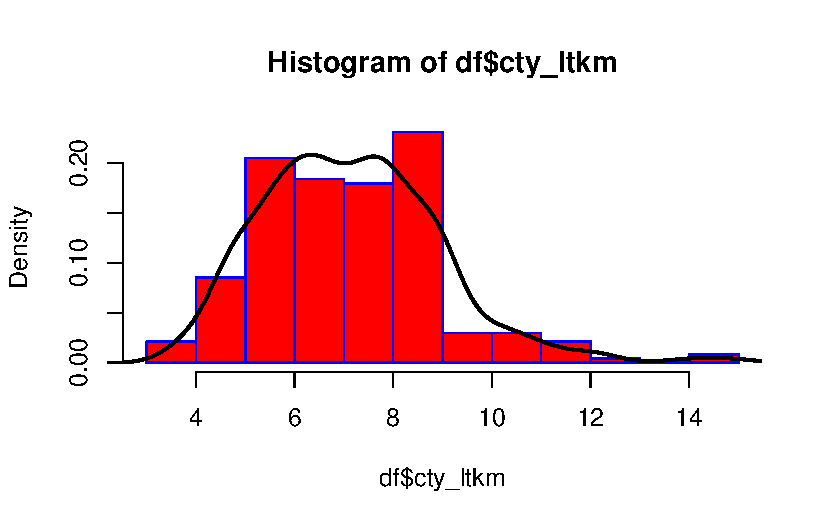
\includegraphics[keepaspectratio]{data_analysis_files/figure-pdf/unnamed-chunk-2-1.pdf}}

\begin{Shaded}
\begin{Highlighting}[]
\FunctionTok{hist}\NormalTok{(df}\SpecialCharTok{$}\NormalTok{hwy\_ltkm,}\AttributeTok{xlim =} \FunctionTok{c}\NormalTok{(}\DecValTok{4}\NormalTok{,}\DecValTok{20}\NormalTok{), }\AttributeTok{ylim =} \FunctionTok{c}\NormalTok{(}\DecValTok{0}\NormalTok{,}\DecValTok{60}\NormalTok{), }\AttributeTok{breaks =} \DecValTok{10}\NormalTok{)}
\end{Highlighting}
\end{Shaded}

\pandocbounded{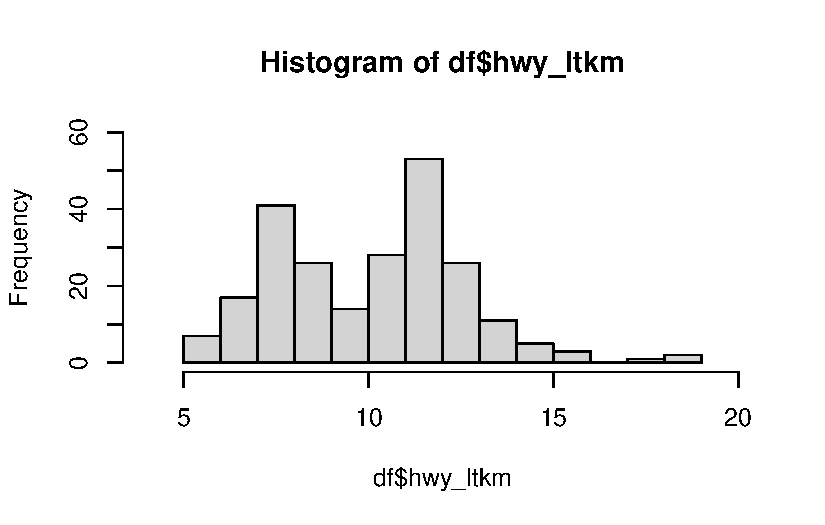
\includegraphics[keepaspectratio]{data_analysis_files/figure-pdf/unnamed-chunk-2-2.pdf}}

\begin{Shaded}
\begin{Highlighting}[]
\CommentTok{\# Boxplot}
\FunctionTok{boxplot}\NormalTok{(df}\SpecialCharTok{$}\NormalTok{cty\_ltkm, }\AttributeTok{main =} \StringTok{"Boxplot cty"}\NormalTok{)}
\end{Highlighting}
\end{Shaded}

\pandocbounded{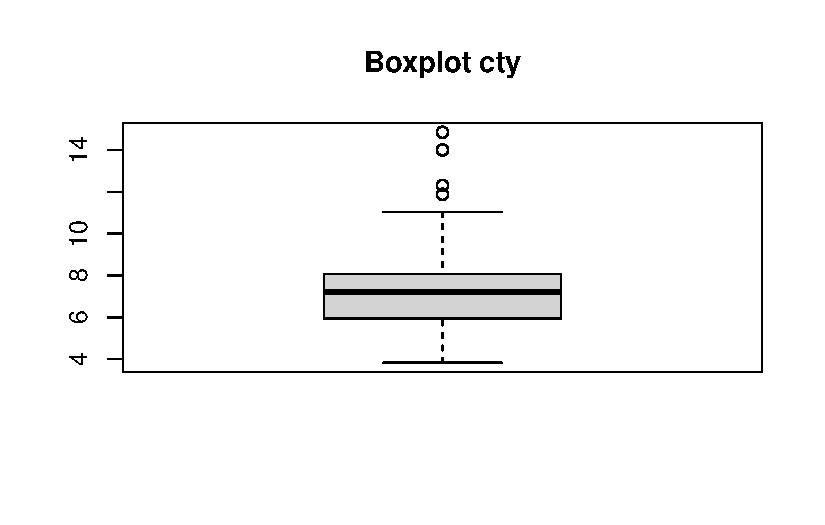
\includegraphics[keepaspectratio]{data_analysis_files/figure-pdf/unnamed-chunk-2-3.pdf}}

\begin{Shaded}
\begin{Highlighting}[]
\FunctionTok{fivenum}\NormalTok{(df}\SpecialCharTok{$}\NormalTok{cty\_ltkm) }\CommentTok{\# minimum, Q1, median, Q3, maximum}
\end{Highlighting}
\end{Shaded}

\begin{verbatim}
[1]  3.820844  5.943536  7.217150  8.066227 14.858839
\end{verbatim}

\begin{Shaded}
\begin{Highlighting}[]
\CommentTok{\# outliers }
\FunctionTok{boxplot}\NormalTok{(df}\SpecialCharTok{$}\NormalTok{cty\_ltkm)}\SpecialCharTok{$}\NormalTok{out}
\end{Highlighting}
\end{Shaded}

\pandocbounded{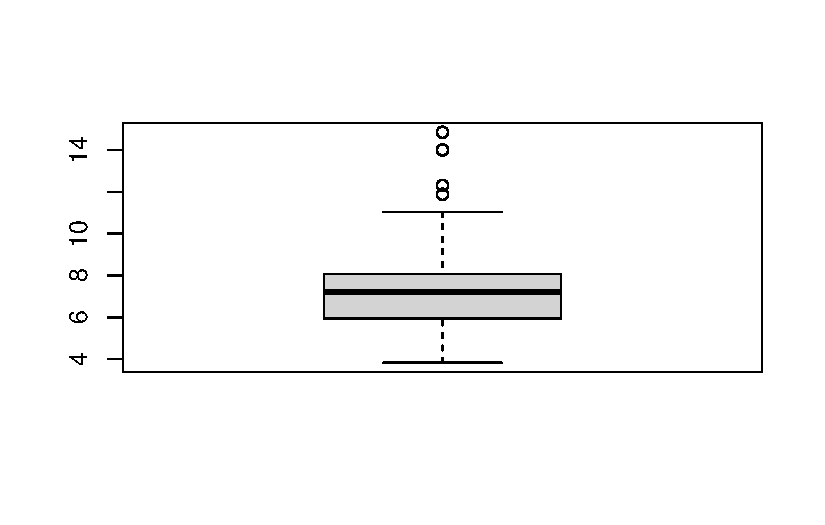
\includegraphics[keepaspectratio]{data_analysis_files/figure-pdf/unnamed-chunk-2-4.pdf}}

\begin{verbatim}
[1] 11.88707 11.88707 14.00976 14.85884 12.31161
\end{verbatim}

\begin{Shaded}
\begin{Highlighting}[]
\CommentTok{\# outliers hangi sıralarda}
\FunctionTok{which}\NormalTok{(df}\SpecialCharTok{$}\NormalTok{cty\_ltkm }\SpecialCharTok{\%in\%} \FunctionTok{boxplot}\NormalTok{(df}\SpecialCharTok{$}\NormalTok{cty\_ltkm)}\SpecialCharTok{$}\NormalTok{out)}
\end{Highlighting}
\end{Shaded}

\begin{verbatim}
[1] 100 197 213 222 223
\end{verbatim}

\begin{Shaded}
\begin{Highlighting}[]
\FunctionTok{boxplot}\NormalTok{(df}\SpecialCharTok{$}\NormalTok{hwy\_ltkm, }\AttributeTok{main =} \StringTok{"Boxplot cty"}\NormalTok{)}
\end{Highlighting}
\end{Shaded}

\pandocbounded{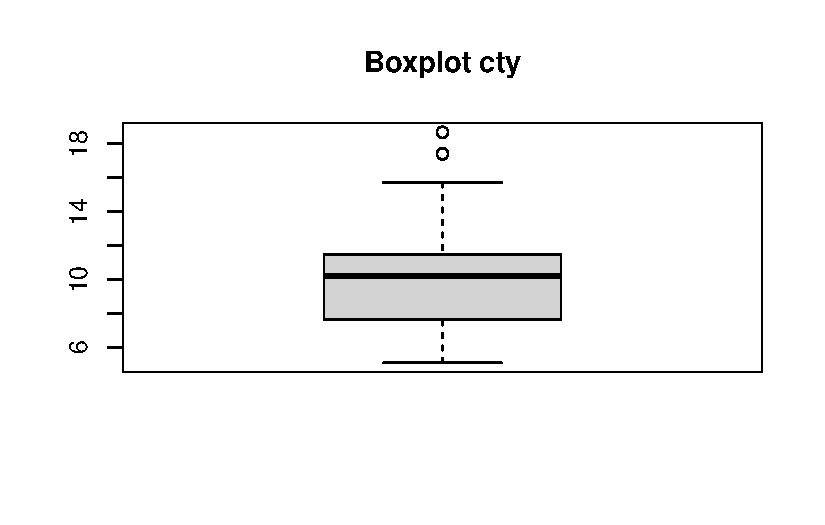
\includegraphics[keepaspectratio]{data_analysis_files/figure-pdf/unnamed-chunk-2-5.pdf}}

\begin{Shaded}
\begin{Highlighting}[]
\FunctionTok{fivenum}\NormalTok{(df}\SpecialCharTok{$}\NormalTok{hwy\_ltkm) }\CommentTok{\# minimum, Q1, median, Q3, maximum}
\end{Highlighting}
\end{Shaded}

\begin{verbatim}
[1]  5.094459  7.641689 10.188918 11.462533 18.679683
\end{verbatim}

\begin{Shaded}
\begin{Highlighting}[]
\FunctionTok{boxplot}\NormalTok{(hwy\_ltkm }\SpecialCharTok{\textasciitilde{}}\NormalTok{ cyl, }\AttributeTok{data =}\NormalTok{ df, }\AttributeTok{xlab =} \StringTok{"Silindir Sayısı"}\NormalTok{,}
   \AttributeTok{ylab =} \StringTok{"Litre Başına KM"}\NormalTok{, }\AttributeTok{main =} \StringTok{"Mileage Data"}\NormalTok{)}
\end{Highlighting}
\end{Shaded}

\pandocbounded{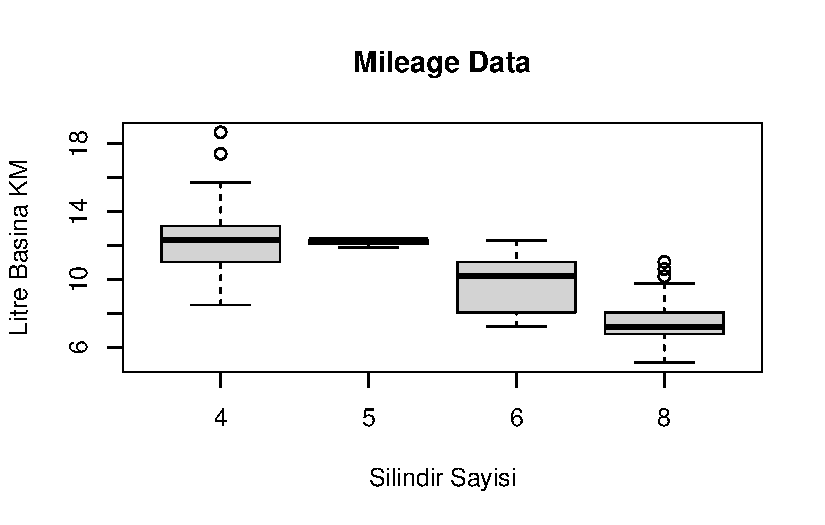
\includegraphics[keepaspectratio]{data_analysis_files/figure-pdf/unnamed-chunk-2-6.pdf}}

\begin{Shaded}
\begin{Highlighting}[]
\FunctionTok{boxplot}\NormalTok{(hwy\_ltkm }\SpecialCharTok{\textasciitilde{}}\NormalTok{ cyl, }\AttributeTok{data =}\NormalTok{ df, }
   \AttributeTok{xlab =} \StringTok{"Silindir Sayısı"}\NormalTok{,}
   \AttributeTok{ylab =} \StringTok{"Litre Başına KM"}\NormalTok{, }
   \AttributeTok{main =} \StringTok{"Mileage Data"}\NormalTok{,}
   \AttributeTok{notch =} \ConstantTok{TRUE}\NormalTok{, }
   \AttributeTok{varwidth =} \ConstantTok{TRUE}\NormalTok{, }
   \AttributeTok{col =} \FunctionTok{c}\NormalTok{(}\StringTok{"green"}\NormalTok{,}\StringTok{"yellow"}\NormalTok{,}\StringTok{"purple"}\NormalTok{,}\StringTok{"blue"}\NormalTok{),}
   \AttributeTok{names =} \FunctionTok{c}\NormalTok{(}\StringTok{"2 Silindir"}\NormalTok{,}\StringTok{"4 Silindir"}\NormalTok{,}\StringTok{"6 Silindir"}\NormalTok{,}\StringTok{"8 Silindir"}\NormalTok{)}
\NormalTok{)}
\end{Highlighting}
\end{Shaded}

\begin{verbatim}
Warning in (function (z, notch = FALSE, width = NULL, varwidth = FALSE, : some
notches went outside hinges ('box'): maybe set notch=FALSE
\end{verbatim}

\pandocbounded{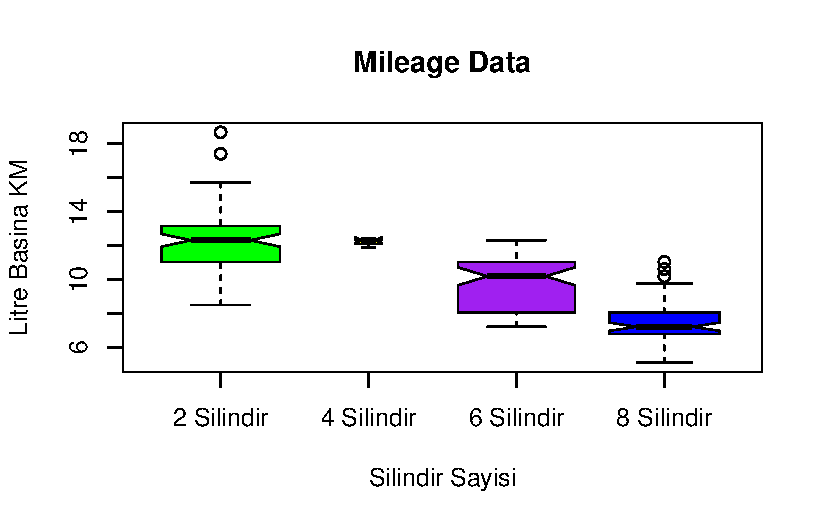
\includegraphics[keepaspectratio]{data_analysis_files/figure-pdf/unnamed-chunk-2-7.pdf}}

\begin{Shaded}
\begin{Highlighting}[]
\CommentTok{\# Sürekli iki değişken incelemek istersek;}

\CommentTok{\# displ ve cty\_ltkm değişkenlerini inceleyelim}
\CommentTok{\# displ motor hacmini ifade ediyor}

\FunctionTok{summary}\NormalTok{(df}\SpecialCharTok{$}\NormalTok{displ)}
\end{Highlighting}
\end{Shaded}

\begin{verbatim}
   Min. 1st Qu.  Median    Mean 3rd Qu.    Max. 
  1.600   2.400   3.300   3.472   4.600   7.000 
\end{verbatim}

\begin{Shaded}
\begin{Highlighting}[]
\FunctionTok{with}\NormalTok{(df,}\FunctionTok{cor}\NormalTok{(displ,cty\_ltkm))}
\end{Highlighting}
\end{Shaded}

\begin{verbatim}
[1] -0.798524
\end{verbatim}

\begin{Shaded}
\begin{Highlighting}[]
\CommentTok{\# motor hacmi ile lt başına km ters ilişkili}

\FunctionTok{plot}\NormalTok{(df}\SpecialCharTok{$}\NormalTok{displ,df}\SpecialCharTok{$}\NormalTok{cty\_ltkm, }
     \AttributeTok{main =} \StringTok{"Motor Hacmi{-} Yakıt Tüketimi Saçılım Grafiği"}\NormalTok{,}
     \AttributeTok{col=}\StringTok{"red"}\NormalTok{,}
     \AttributeTok{xlab =} \StringTok{"Motor Hacmi"}\NormalTok{,}
     \AttributeTok{ylab =} \StringTok{"Yakıt Tüketimi"}\NormalTok{)}
\end{Highlighting}
\end{Shaded}

\pandocbounded{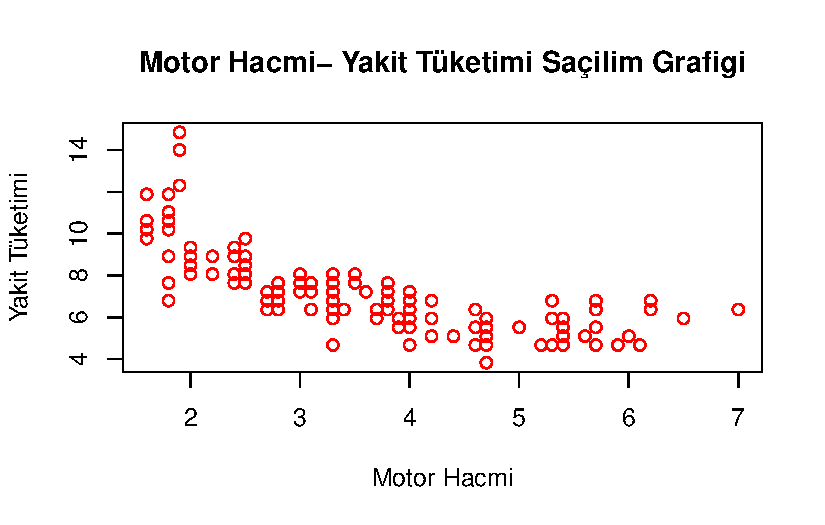
\includegraphics[keepaspectratio]{data_analysis_files/figure-pdf/unnamed-chunk-2-8.pdf}}

\begin{Shaded}
\begin{Highlighting}[]
\CommentTok{\# birden fazla değişkenin saçılım grafiği}
\FunctionTok{pairs}\NormalTok{(}\SpecialCharTok{\textasciitilde{}}\NormalTok{hwy\_ltkm}\SpecialCharTok{+}\NormalTok{cty\_ltkm}\SpecialCharTok{+}\NormalTok{displ}\SpecialCharTok{+}\NormalTok{cyl,}\AttributeTok{data =}\NormalTok{ df,}\AttributeTok{main =} \StringTok{"Scatterplot Matrix"}\NormalTok{)}
\end{Highlighting}
\end{Shaded}

\pandocbounded{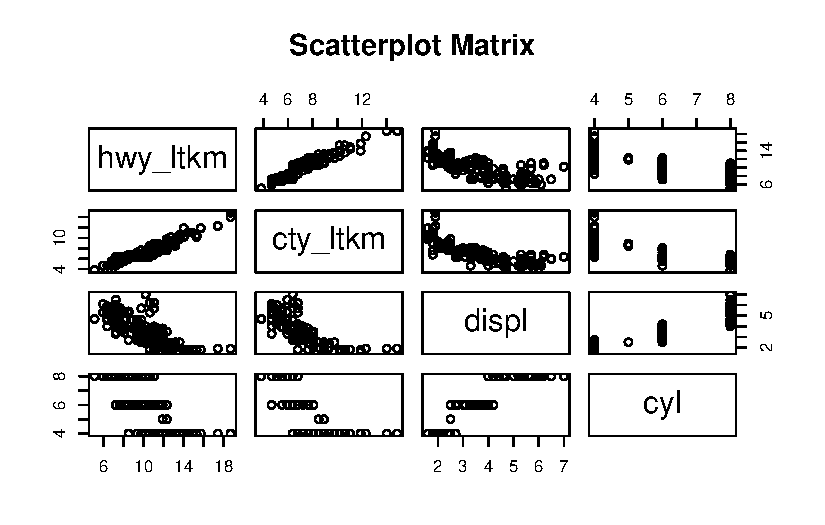
\includegraphics[keepaspectratio]{data_analysis_files/figure-pdf/unnamed-chunk-2-9.pdf}}

\section*{Kategorik Değişkenler}\label{kategorik-deux11fiux15fkenler}
\addcontentsline{toc}{section}{Kategorik Değişkenler}

\markright{Kategorik Değişkenler}

Veri analizi sürecinde, kategorik değişkenler (veya gruplar) genellikle
çok önemli bir rol oynar. Kategorik değişkenler, belirli bir sınıfı veya
kategoriyi temsil eden değişkenlerdir ve tipik olarak metin veya
sembollerle ifade edilirler. Örnek olarak, cinsiyet, eğitim seviyesi,
ürün kategorileri gibi değişkenler kategorik değişkenlere örnektir.
Kategorik değişkenlerin analizi, bu değişkenlerin içindeki örüntüleri,
dağılımları ve ilişkileri anlamamıza yardımcı olur. Aşağıda, kategorik
değişkenlerin analizi için izlenebilecek temel adımları bulabilirsiniz:

\begin{enumerate}
\def\labelenumi{\arabic{enumi}.}
\item
  \textbf{Frekans Tabloları ve Görselleştirme:} Kategorik değişkenlerin
  frekans tablolarını ve grafiklerini oluşturarak, her kategori veya
  sınıfın veri setinde ne kadar sık görüldüğünü anlayabilirsiniz.
  Örneğin, bar grafikleri, pasta grafikleri veya çubuk grafikleri
  kullanarak kategori frekanslarını görselleştirebilirsiniz.
  \textbf{\texttt{summary()}} ve \textbf{\texttt{table()}} gibi R
  fonksiyonları ile bu verileri inceleyebilirsiniz.
\item
  \textbf{İlişkileri İnceleme:} Kategorik değişkenler arasındaki
  ilişkileri anlamak önemlidir. İki kategorik değişken arasındaki
  ilişkiyi değerlendirmek için çapraz tablolar (cross-tabulation) ve
  ki-kare (chi-squared) istatistiksel testleri kullanabilirsiniz. Bu
  testler, iki değişken arasındaki bağımlılığı değerlendirmek için
  kullanılır.
\item
  \textbf{İstatistiksel Testler:} Kategorik değişkenlerin analizi
  sırasında, gruplar arasındaki farkları değerlendirmek için hipotez
  testleri kullanabilirsiniz. İki kategorik değişken arasındaki
  ilişkinin istatistiksel olarak anlamlı olup olmadığını belirlemek için
  ki-kare testi veya Fisher'in kesin testi gibi testler
  kullanabilirsiniz. Ayrıca ANOVA gibi testler, bir kategorik değişkenin
  birden fazla grup üzerindeki etkisini değerlendirmek için
  kullanılabilir.
\item
  \textbf{Veri Görselleştirme:} Kategorik değişkenlerin analizinde,
  gruplar arasındaki farkları daha iyi anlamak için grafikler
  kullanabilirsiniz. Bar grafikleri, grupların frekanslarını
  görselleştirmek için sıklıkla kullanılırken, gruplar arasındaki
  ilişkiyi anlamak için mozaik grafikleri veya heatmap'leri de
  kullanabilirsiniz.
\end{enumerate}

Kategorik değişkenlerin analizi, veri setinizin içindeki desenleri ve
ilişkileri anlamanıza yardımcı olur. Bu analiz, kararlarınızı
desteklemek ve veriyi daha iyi anlamak için önemlidir. R programlama
dili, kategorik değişkenlerin analizi için bir dizi kullanışlı fonksiyon
ve paket sunar. Bu adımları takip ederek, veri analiz projelerinizde
kategorik değişkenleri etkili bir şekilde analiz edebilirsiniz.

\begin{Shaded}
\begin{Highlighting}[]
\CommentTok{\# class ve trans değişkenlerine bakalım}
\CommentTok{\# class araç sınıfı, trans ise vites türünü ifade ediyor.}

\FunctionTok{summary}\NormalTok{(df}\SpecialCharTok{$}\NormalTok{class)}
\end{Highlighting}
\end{Shaded}

\begin{verbatim}
   2seater    compact    midsize    minivan     pickup subcompact        suv 
         5         47         41         11         33         35         62 
\end{verbatim}

\begin{Shaded}
\begin{Highlighting}[]
\FunctionTok{table}\NormalTok{(df}\SpecialCharTok{$}\NormalTok{class)}
\end{Highlighting}
\end{Shaded}

\begin{verbatim}

   2seater    compact    midsize    minivan     pickup subcompact        suv 
         5         47         41         11         33         35         62 
\end{verbatim}

\begin{Shaded}
\begin{Highlighting}[]
\FunctionTok{xtabs}\NormalTok{(}\SpecialCharTok{\textasciitilde{}}\NormalTok{class,}\AttributeTok{data=}\NormalTok{df)}
\end{Highlighting}
\end{Shaded}

\begin{verbatim}
class
   2seater    compact    midsize    minivan     pickup subcompact        suv 
         5         47         41         11         33         35         62 
\end{verbatim}

\begin{Shaded}
\begin{Highlighting}[]
\FunctionTok{table}\NormalTok{(df}\SpecialCharTok{$}\NormalTok{trans)}
\end{Highlighting}
\end{Shaded}

\begin{verbatim}

  auto(av)   auto(l3)   auto(l4)   auto(l5)   auto(l6)   auto(s4)   auto(s5) 
         5          2         83         39          6          3          3 
  auto(s6) manual(m5) manual(m6) 
        16         58         19 
\end{verbatim}

\begin{Shaded}
\begin{Highlighting}[]
\FunctionTok{prop.table}\NormalTok{(}\FunctionTok{table}\NormalTok{(df}\SpecialCharTok{$}\NormalTok{class))}
\end{Highlighting}
\end{Shaded}

\begin{verbatim}

   2seater    compact    midsize    minivan     pickup subcompact        suv 
0.02136752 0.20085470 0.17521368 0.04700855 0.14102564 0.14957265 0.26495726 
\end{verbatim}

\begin{Shaded}
\begin{Highlighting}[]
\NormalTok{tab }\OtherTok{\textless{}{-}} \FunctionTok{table}\NormalTok{(df}\SpecialCharTok{$}\NormalTok{class)}
\FunctionTok{barplot}\NormalTok{(tab,}\AttributeTok{col=}\StringTok{"blue"}\NormalTok{,}\AttributeTok{border=}\StringTok{"red"}\NormalTok{)}
\end{Highlighting}
\end{Shaded}

\pandocbounded{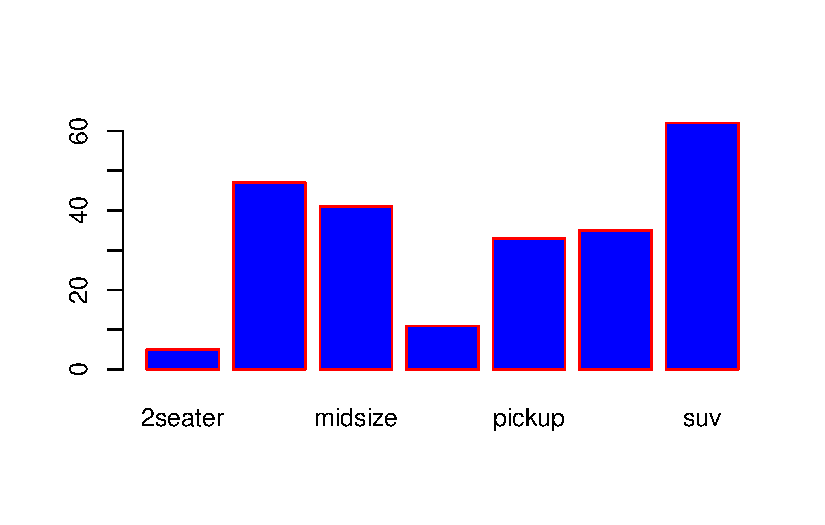
\includegraphics[keepaspectratio]{data_analysis_files/figure-pdf/unnamed-chunk-3-1.pdf}}

\begin{Shaded}
\begin{Highlighting}[]
\FunctionTok{pie}\NormalTok{(tab)}
\end{Highlighting}
\end{Shaded}

\pandocbounded{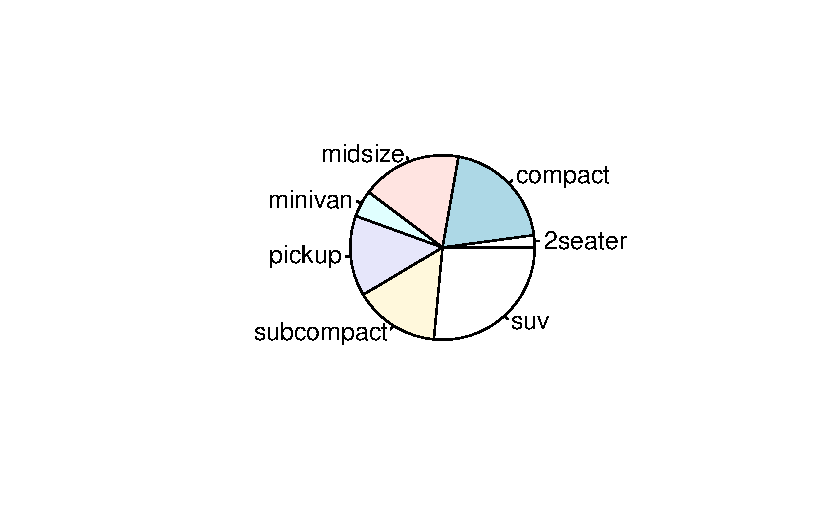
\includegraphics[keepaspectratio]{data_analysis_files/figure-pdf/unnamed-chunk-3-2.pdf}}

\begin{Shaded}
\begin{Highlighting}[]
\FunctionTok{par}\NormalTok{(}\AttributeTok{mfrow =} \FunctionTok{c}\NormalTok{(}\DecValTok{1}\NormalTok{, }\DecValTok{2}\NormalTok{))}
\FunctionTok{barplot}\NormalTok{(tab)}
\FunctionTok{pie}\NormalTok{(tab)}
\end{Highlighting}
\end{Shaded}

\pandocbounded{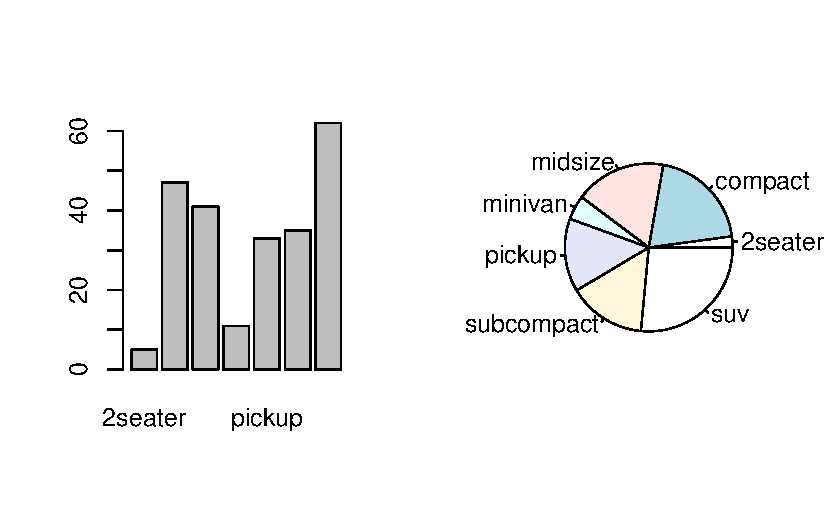
\includegraphics[keepaspectratio]{data_analysis_files/figure-pdf/unnamed-chunk-3-3.pdf}}

\begin{Shaded}
\begin{Highlighting}[]
\CommentTok{\# Kategorik iki değişken incelemek istersek;}

\FunctionTok{xtabs}\NormalTok{(}\SpecialCharTok{\textasciitilde{}}\NormalTok{trans}\SpecialCharTok{+}\NormalTok{class,}\AttributeTok{data=}\NormalTok{df)}
\end{Highlighting}
\end{Shaded}

\begin{verbatim}
            class
trans        2seater compact midsize minivan pickup subcompact suv
  auto(av)         0       2       3       0      0          0   0
  auto(l3)         0       1       0       1      0          0   0
  auto(l4)         1       8      14       8     12         11  29
  auto(l5)         0       4       5       0      8          4  18
  auto(l6)         0       0       0       2      0          0   4
  auto(s4)         0       2       1       0      0          0   0
  auto(s5)         0       2       0       0      0          0   1
  auto(s6)         1       5       6       0      0          1   3
  manual(m5)       0      18       9       0      8         16   7
  manual(m6)       3       5       3       0      5          3   0
\end{verbatim}

\begin{Shaded}
\begin{Highlighting}[]
\FunctionTok{prop.table}\NormalTok{(}\FunctionTok{table}\NormalTok{(df}\SpecialCharTok{$}\NormalTok{year,df}\SpecialCharTok{$}\NormalTok{class),}\DecValTok{1}\NormalTok{) }\CommentTok{\# satır toplamları 1\textquotesingle{} eşittir}
\end{Highlighting}
\end{Shaded}

\begin{verbatim}
      
          2seater    compact    midsize    minivan     pickup subcompact
  1999 0.01709402 0.21367521 0.17094017 0.05128205 0.13675214 0.16239316
  2008 0.02564103 0.18803419 0.17948718 0.04273504 0.14529915 0.13675214
      
              suv
  1999 0.24786325
  2008 0.28205128
\end{verbatim}

\begin{Shaded}
\begin{Highlighting}[]
\FunctionTok{prop.table}\NormalTok{(}\FunctionTok{table}\NormalTok{(df}\SpecialCharTok{$}\NormalTok{year,df}\SpecialCharTok{$}\NormalTok{class),}\DecValTok{2}\NormalTok{) }\CommentTok{\# sütun toplamları 1\textquotesingle{} eşittir}
\end{Highlighting}
\end{Shaded}

\begin{verbatim}
      
         2seater   compact   midsize   minivan    pickup subcompact       suv
  1999 0.4000000 0.5319149 0.4878049 0.5454545 0.4848485  0.5428571 0.4677419
  2008 0.6000000 0.4680851 0.5121951 0.4545455 0.5151515  0.4571429 0.5322581
\end{verbatim}

\begin{Shaded}
\begin{Highlighting}[]
\FunctionTok{proportions}\NormalTok{(}\FunctionTok{xtabs}\NormalTok{(}\SpecialCharTok{\textasciitilde{}}\NormalTok{ manufacturer }\SpecialCharTok{+}\NormalTok{ year, }\AttributeTok{data =}\NormalTok{ df), }\DecValTok{1}\NormalTok{)}
\end{Highlighting}
\end{Shaded}

\begin{verbatim}
            year
manufacturer      1999      2008
  audi       0.5000000 0.5000000
  chevrolet  0.3684211 0.6315789
  dodge      0.4324324 0.5675676
  ford       0.6000000 0.4000000
  honda      0.5555556 0.4444444
  hyundai    0.4285714 0.5714286
  jeep       0.2500000 0.7500000
  land rover 0.5000000 0.5000000
  lincoln    0.6666667 0.3333333
  mercury    0.5000000 0.5000000
  nissan     0.4615385 0.5384615
  pontiac    0.6000000 0.4000000
  subaru     0.4285714 0.5714286
  toyota     0.5882353 0.4117647
  volkswagen 0.5925926 0.4074074
\end{verbatim}

\begin{Shaded}
\begin{Highlighting}[]
\CommentTok{\# araç sınıfı ile drv değişkenine birlikte bakalım}
\CommentTok{\# f = front{-}wheel drive (önden çekiş), }
\CommentTok{\# r = rear wheel drive (arkadan çekiş), }
\CommentTok{\# 4 = 4wd (4 çeker)}

\FunctionTok{plot}\NormalTok{(class }\SpecialCharTok{\textasciitilde{}} \FunctionTok{factor}\NormalTok{(drv), }\AttributeTok{data =}\NormalTok{ df)}
\end{Highlighting}
\end{Shaded}

\pandocbounded{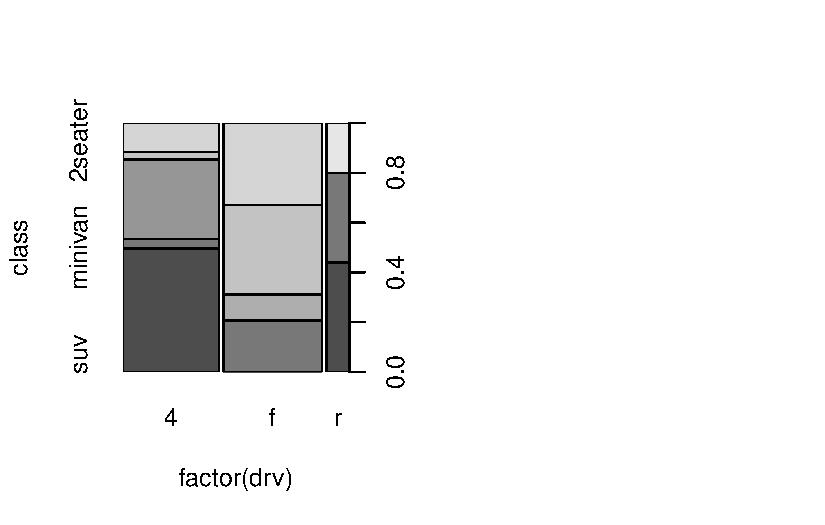
\includegraphics[keepaspectratio]{data_analysis_files/figure-pdf/unnamed-chunk-3-4.pdf}}

Eğer hem sürekli hem de kategorik değişkenleri incelemek istersek,
benzer şekilde görselleştirme ve kategoriler arasında merkezi eğilim
ölçüleri hesaplanabilir. Bunlar dışında uygun istatistiksel testler de
gerçekleştirilebilir.

\begin{Shaded}
\begin{Highlighting}[]
\CommentTok{\# Silindir düzeyinde yakıt tüketimi }
\FunctionTok{tapply}\NormalTok{(df}\SpecialCharTok{$}\NormalTok{cty\_ltkm, df}\SpecialCharTok{$}\NormalTok{cyl, mean)}
\end{Highlighting}
\end{Shaded}

\begin{verbatim}
       4        5        6        8 
8.920545 8.703034 6.883968 5.337052 
\end{verbatim}

\begin{Shaded}
\begin{Highlighting}[]
\CommentTok{\# Same using aggregate()}
\FunctionTok{aggregate}\NormalTok{(cty\_ltkm }\SpecialCharTok{\textasciitilde{}}\NormalTok{ cyl, }\AttributeTok{data =}\NormalTok{ df, }\AttributeTok{FUN =}\NormalTok{ mean)}
\end{Highlighting}
\end{Shaded}

\begin{verbatim}
  cyl cty_ltkm
1   4 8.920545
2   5 8.703034
3   6 6.883968
4   8 5.337052
\end{verbatim}

\begin{Shaded}
\begin{Highlighting}[]
\FunctionTok{boxplot}\NormalTok{(cty\_ltkm }\SpecialCharTok{\textasciitilde{}}\NormalTok{ cyl, }\AttributeTok{data =}\NormalTok{ df)}
\end{Highlighting}
\end{Shaded}

\pandocbounded{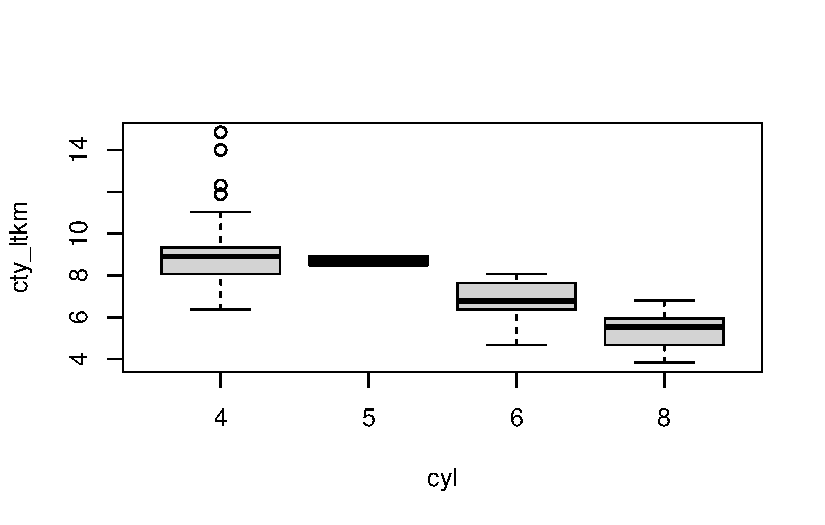
\includegraphics[keepaspectratio]{data_analysis_files/figure-pdf/unnamed-chunk-4-1.pdf}}

\section*{Zaman Serileri}\label{zaman-serileri}
\addcontentsline{toc}{section}{Zaman Serileri}

\markright{Zaman Serileri}

R programlama dili, zaman serileri analizi için kapsamlı bir dizi
fonksiyon ve paket sunar. Zaman serileri analizi, zaman içindeki veri
noktalarının örüntülerini ve trendlerini incelemeyi amaçlar. R'de zaman
serileri ile çalışmak için \textbf{\texttt{ts}} (time series) nesnesi
kullanılır. Bu nesne, zaman serisi verilerini zaman dilimleri (örneğin
aylar, yıllar) veya tarihler ile ilişkilendirerek işlem yapmanıza olanak
tanır.

\begin{Shaded}
\begin{Highlighting}[]
\NormalTok{AirPassengers}
\end{Highlighting}
\end{Shaded}

\begin{verbatim}
     Jan Feb Mar Apr May Jun Jul Aug Sep Oct Nov Dec
1949 112 118 132 129 121 135 148 148 136 119 104 118
1950 115 126 141 135 125 149 170 170 158 133 114 140
1951 145 150 178 163 172 178 199 199 184 162 146 166
1952 171 180 193 181 183 218 230 242 209 191 172 194
1953 196 196 236 235 229 243 264 272 237 211 180 201
1954 204 188 235 227 234 264 302 293 259 229 203 229
1955 242 233 267 269 270 315 364 347 312 274 237 278
1956 284 277 317 313 318 374 413 405 355 306 271 306
1957 315 301 356 348 355 422 465 467 404 347 305 336
1958 340 318 362 348 363 435 491 505 404 359 310 337
1959 360 342 406 396 420 472 548 559 463 407 362 405
1960 417 391 419 461 472 535 622 606 508 461 390 432
\end{verbatim}

\begin{Shaded}
\begin{Highlighting}[]
\FunctionTok{class}\NormalTok{(AirPassengers)}
\end{Highlighting}
\end{Shaded}

\begin{verbatim}
[1] "ts"
\end{verbatim}

\begin{Shaded}
\begin{Highlighting}[]
\FunctionTok{diff}\NormalTok{(AirPassengers) }\CommentTok{\# fark alma}
\end{Highlighting}
\end{Shaded}

\begin{verbatim}
      Jan  Feb  Mar  Apr  May  Jun  Jul  Aug  Sep  Oct  Nov  Dec
1949         6   14   -3   -8   14   13    0  -12  -17  -15   14
1950   -3   11   15   -6  -10   24   21    0  -12  -25  -19   26
1951    5    5   28  -15    9    6   21    0  -15  -22  -16   20
1952    5    9   13  -12    2   35   12   12  -33  -18  -19   22
1953    2    0   40   -1   -6   14   21    8  -35  -26  -31   21
1954    3  -16   47   -8    7   30   38   -9  -34  -30  -26   26
1955   13   -9   34    2    1   45   49  -17  -35  -38  -37   41
1956    6   -7   40   -4    5   56   39   -8  -50  -49  -35   35
1957    9  -14   55   -8    7   67   43    2  -63  -57  -42   31
1958    4  -22   44  -14   15   72   56   14 -101  -45  -49   27
1959   23  -18   64  -10   24   52   76   11  -96  -56  -45   43
1960   12  -26   28   42   11   63   87  -16  -98  -47  -71   42
\end{verbatim}

\begin{Shaded}
\begin{Highlighting}[]
\NormalTok{stats}\SpecialCharTok{::}\FunctionTok{lag}\NormalTok{(AirPassengers,}\SpecialCharTok{{-}}\DecValTok{1}\NormalTok{) }\CommentTok{\# 1. gecikmesini alma}
\end{Highlighting}
\end{Shaded}

\begin{verbatim}
     Jan Feb Mar Apr May Jun Jul Aug Sep Oct Nov Dec
1949     112 118 132 129 121 135 148 148 136 119 104
1950 118 115 126 141 135 125 149 170 170 158 133 114
1951 140 145 150 178 163 172 178 199 199 184 162 146
1952 166 171 180 193 181 183 218 230 242 209 191 172
1953 194 196 196 236 235 229 243 264 272 237 211 180
1954 201 204 188 235 227 234 264 302 293 259 229 203
1955 229 242 233 267 269 270 315 364 347 312 274 237
1956 278 284 277 317 313 318 374 413 405 355 306 271
1957 306 315 301 356 348 355 422 465 467 404 347 305
1958 336 340 318 362 348 363 435 491 505 404 359 310
1959 337 360 342 406 396 420 472 548 559 463 407 362
1960 405 417 391 419 461 472 535 622 606 508 461 390
1961 432                                            
\end{verbatim}

\begin{Shaded}
\begin{Highlighting}[]
\FunctionTok{plot}\NormalTok{(AirPassengers,}\AttributeTok{type =} \StringTok{"p"}\NormalTok{, }\AttributeTok{col =} \StringTok{"red"}\NormalTok{) }\CommentTok{\# points}
\end{Highlighting}
\end{Shaded}

\pandocbounded{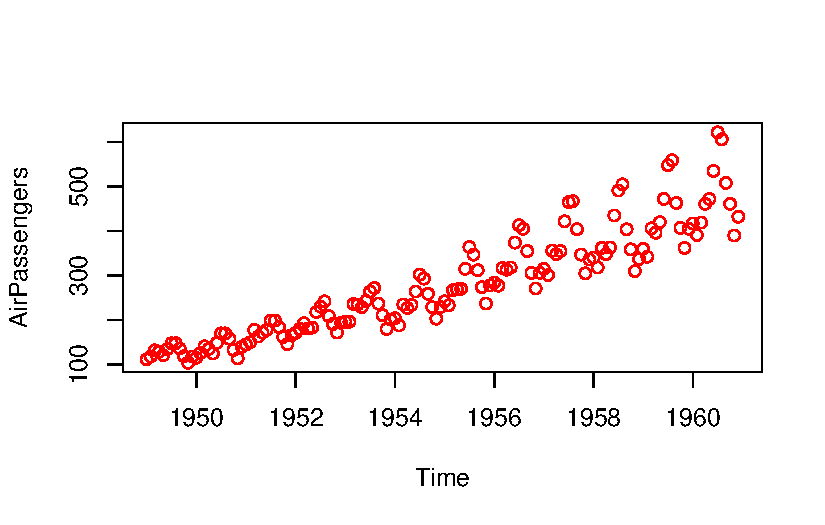
\includegraphics[keepaspectratio]{data_analysis_files/figure-pdf/unnamed-chunk-5-1.pdf}}

\begin{Shaded}
\begin{Highlighting}[]
\FunctionTok{plot}\NormalTok{(AirPassengers,}\AttributeTok{type =} \StringTok{"l"}\NormalTok{, }\AttributeTok{col =} \StringTok{"red"}\NormalTok{) }\CommentTok{\# line}
\end{Highlighting}
\end{Shaded}

\pandocbounded{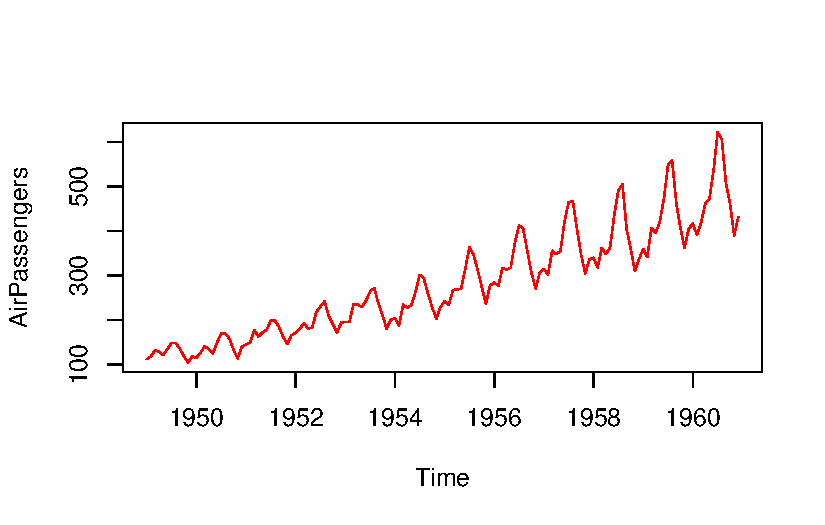
\includegraphics[keepaspectratio]{data_analysis_files/figure-pdf/unnamed-chunk-5-2.pdf}}

\begin{Shaded}
\begin{Highlighting}[]
\FunctionTok{plot}\NormalTok{(AirPassengers,}\AttributeTok{type =} \StringTok{"o"}\NormalTok{, }\AttributeTok{col =} \StringTok{"red"}\NormalTok{) }\CommentTok{\# points and line}
\end{Highlighting}
\end{Shaded}

\pandocbounded{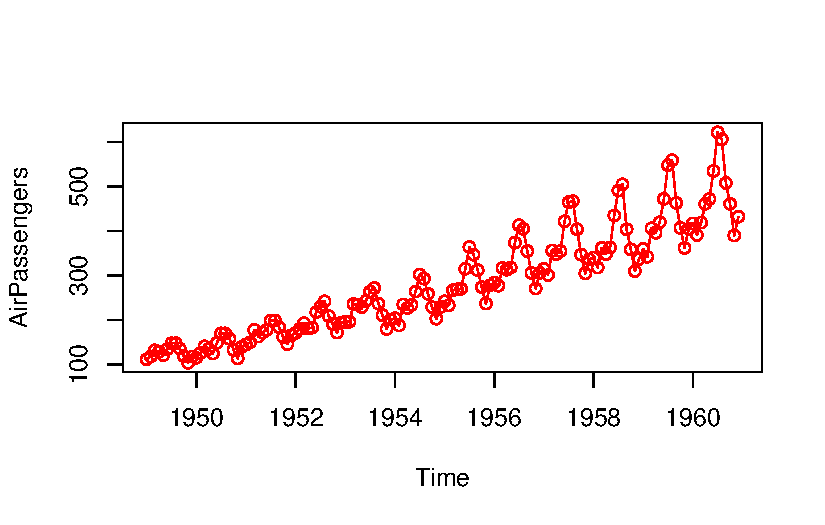
\includegraphics[keepaspectratio]{data_analysis_files/figure-pdf/unnamed-chunk-5-3.pdf}}

\begin{Shaded}
\begin{Highlighting}[]
\FunctionTok{plot}\NormalTok{(}\FunctionTok{log}\NormalTok{(AirPassengers),}\AttributeTok{type =} \StringTok{"l"}\NormalTok{, }\AttributeTok{col =} \StringTok{"red"}\NormalTok{) }\CommentTok{\# line}
\end{Highlighting}
\end{Shaded}

\pandocbounded{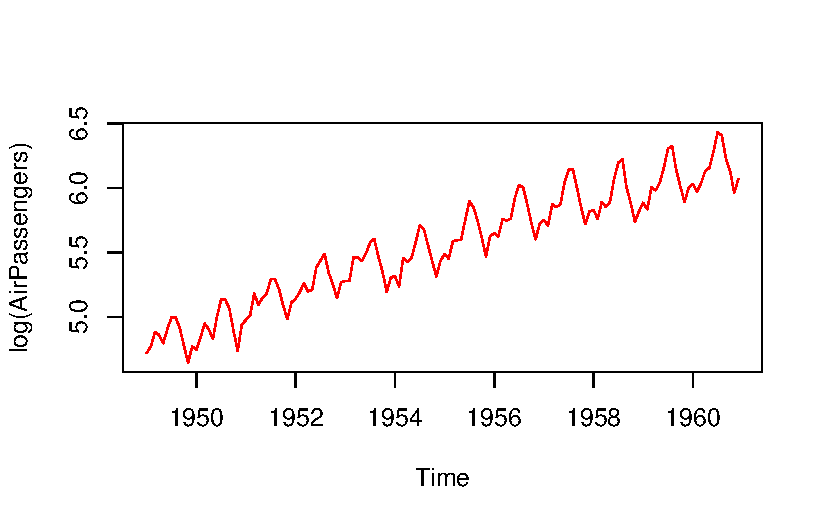
\includegraphics[keepaspectratio]{data_analysis_files/figure-pdf/unnamed-chunk-5-4.pdf}}

\begin{Shaded}
\begin{Highlighting}[]
\FunctionTok{plot}\NormalTok{(}\FunctionTok{diff}\NormalTok{(AirPassengers),}\AttributeTok{type =} \StringTok{"l"}\NormalTok{, }\AttributeTok{col =} \StringTok{"red"}\NormalTok{) }\CommentTok{\# line}
\end{Highlighting}
\end{Shaded}

\pandocbounded{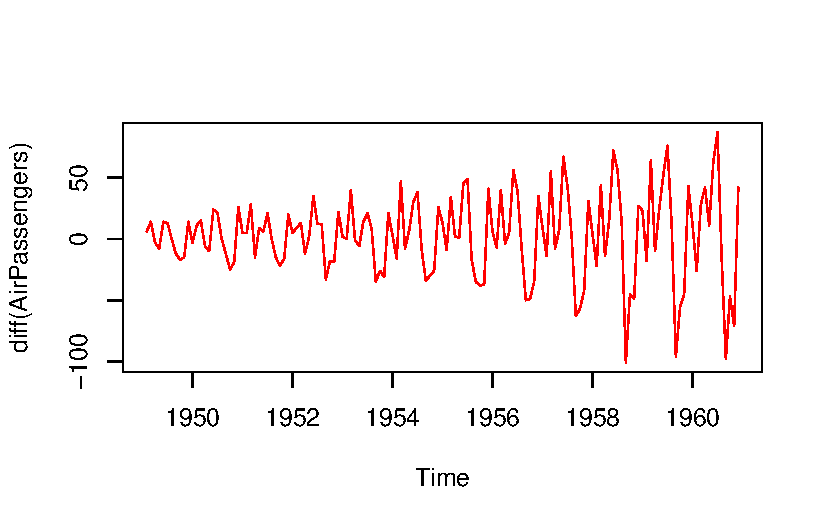
\includegraphics[keepaspectratio]{data_analysis_files/figure-pdf/unnamed-chunk-5-5.pdf}}

\begin{Shaded}
\begin{Highlighting}[]
\FunctionTok{plot}\NormalTok{(}\FunctionTok{diff}\NormalTok{(}\FunctionTok{log}\NormalTok{(AirPassengers)),}\AttributeTok{type =} \StringTok{"l"}\NormalTok{, }\AttributeTok{col =} \StringTok{"red"}\NormalTok{) }\CommentTok{\# line}
\end{Highlighting}
\end{Shaded}

\pandocbounded{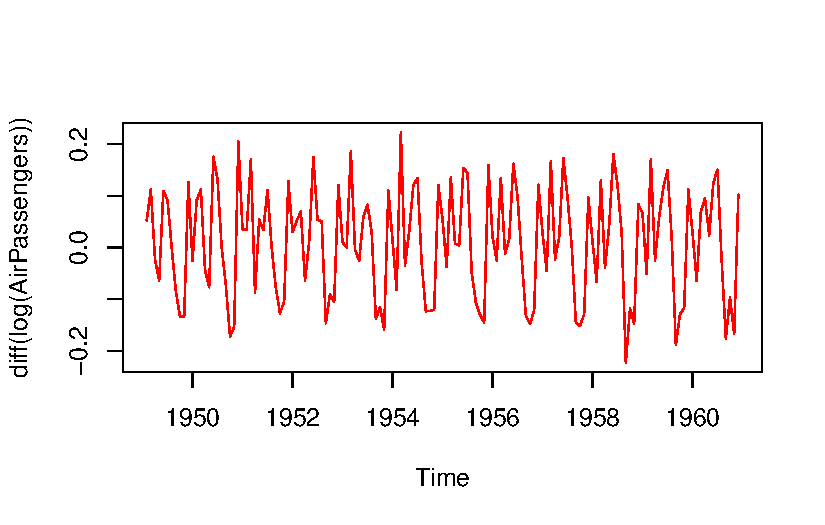
\includegraphics[keepaspectratio]{data_analysis_files/figure-pdf/unnamed-chunk-5-6.pdf}}

\begin{Shaded}
\begin{Highlighting}[]
\CommentTok{\# çoklu zaman serisi}
\NormalTok{ts }\OtherTok{\textless{}{-}} \FunctionTok{ts}\NormalTok{(}\FunctionTok{rnorm}\NormalTok{(}\FunctionTok{length}\NormalTok{(AirPassengers),}\DecValTok{250}\NormalTok{,}\DecValTok{100}\NormalTok{),}\AttributeTok{start =} \FunctionTok{c}\NormalTok{(}\DecValTok{1949}\NormalTok{,}\DecValTok{1}\NormalTok{),}\AttributeTok{frequency=}\DecValTok{12}\NormalTok{)}
\NormalTok{ts}
\end{Highlighting}
\end{Shaded}

\begin{verbatim}
             Jan         Feb         Mar         Apr         May         Jun
1949 145.2017165 269.7951870 234.8787317 230.0133668 205.5590809 118.8315899
1950 339.0633058  68.4032542 246.7111303 270.3900577 428.7644986 300.0435206
1951 277.6001961 342.3087622 246.1456238 215.6586837 221.6655818 172.3166038
1952 340.3101718 264.7716978 350.9422973 292.1653084 410.3503035 169.1791786
1953 439.8520533 230.2519209 213.5163938 310.2337284 161.2296974 144.1771314
1954 298.8943293 341.6161829 492.5641918 297.4697422 317.0638169 189.2761552
1955 323.8125557 312.7812018 359.5417110 353.5327135 302.8520309 229.7677054
1956 251.2001645 147.1260360 205.2338661 314.4371532 403.5364768 239.4670641
1957 304.3718628 127.5730548 275.6091491 186.7188849 169.4249652 130.7616082
1958 189.3159013 343.9958762 333.6645492 301.6084291  -0.9093919 136.6360192
1959  80.3983576 278.9067292 104.6260808 350.1998198 190.9027762 -46.3743321
1960 271.0776239 331.6095728 299.0358092 233.1109986  30.0648761 122.6320219
             Jul         Aug         Sep         Oct         Nov         Dec
1949 221.3799969 267.9875347 194.8686555 308.6391832 364.5836330 316.5542779
1950  21.3652096 106.2477157 336.0682277 399.6864101 223.0876310 176.4536184
1951 385.3460747 295.0788245 131.9572589 228.0421114 198.9897227 479.6002073
1952 -14.7516021 245.5642759 183.4378281 264.9440177 379.2828575 178.5440406
1953 204.2645721 438.1762251 272.3289874 366.5001435 323.4352780 239.0866085
1954 309.8840386 165.2782586 -12.6385821 150.0082023 346.5626358 310.3603897
1955 376.5482299 431.8897853 313.1285770 302.9055770 191.3786542 417.9327630
1956 197.9052268 455.9254419 250.4434082 216.7521632 379.8399273 211.7333715
1957 258.5248175 216.8793924 448.8080975 209.4588869 422.2126087 254.5878345
1958 202.0613804 106.8611643 352.7157212  96.7484573 334.0313627 244.5209770
1959 488.8618150  30.0365360  22.1129213 262.2085987 161.5693172 341.9274893
1960 194.4131436 344.4658508 185.4200543 332.7690120 237.2105295 215.7343850
\end{verbatim}

\begin{Shaded}
\begin{Highlighting}[]
\FunctionTok{plot}\NormalTok{(AirPassengers,}\AttributeTok{type =} \StringTok{"l"}\NormalTok{,}\AttributeTok{col =} \StringTok{"red"}\NormalTok{)}
\FunctionTok{lines}\NormalTok{(ts, }\AttributeTok{type =} \StringTok{"l"}\NormalTok{, }\AttributeTok{col =} \StringTok{"blue"}\NormalTok{)}
\end{Highlighting}
\end{Shaded}

\pandocbounded{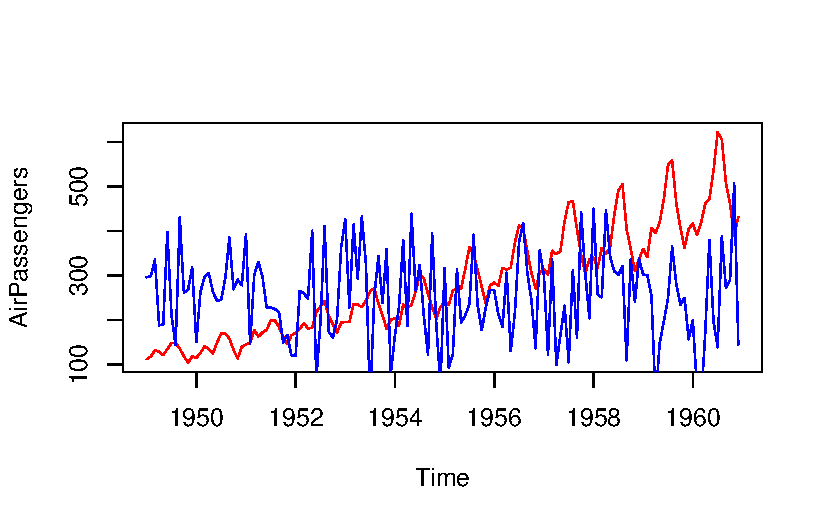
\includegraphics[keepaspectratio]{data_analysis_files/figure-pdf/unnamed-chunk-5-7.pdf}}

\begin{Shaded}
\begin{Highlighting}[]
\CommentTok{\# yüzde değişim}
\NormalTok{growth }\OtherTok{\textless{}{-}}\NormalTok{ AirPassengers}\SpecialCharTok{/}\NormalTok{stats}\SpecialCharTok{::}\FunctionTok{lag}\NormalTok{(AirPassengers,}\SpecialCharTok{{-}}\DecValTok{1}\NormalTok{)}\SpecialCharTok{*}\DecValTok{100{-}100}
\NormalTok{growth}
\end{Highlighting}
\end{Shaded}

\begin{verbatim}
             Jan         Feb         Mar         Apr         May         Jun
1949               5.3571429  11.8644068  -2.2727273  -6.2015504  11.5702479
1950  -2.5423729   9.5652174  11.9047619  -4.2553191  -7.4074074  19.2000000
1951   3.5714286   3.4482759  18.6666667  -8.4269663   5.5214724   3.4883721
1952   3.0120482   5.2631579   7.2222222  -6.2176166   1.1049724  19.1256831
1953   1.0309278   0.0000000  20.4081633  -0.4237288  -2.5531915   6.1135371
1954   1.4925373  -7.8431373  25.0000000  -3.4042553   3.0837004  12.8205128
1955   5.6768559  -3.7190083  14.5922747   0.7490637   0.3717472  16.6666667
1956   2.1582734  -2.4647887  14.4404332  -1.2618297   1.5974441  17.6100629
1957   2.9411765  -4.4444444  18.2724252  -2.2471910   2.0114943  18.8732394
1958   1.1904762  -6.4705882  13.8364780  -3.8674033   4.3103448  19.8347107
1959   6.8249258  -5.0000000  18.7134503  -2.4630542   6.0606061  12.3809524
1960   2.9629630  -6.2350120   7.1611253  10.0238663   2.3861171  13.3474576
             Jul         Aug         Sep         Oct         Nov         Dec
1949   9.6296296   0.0000000  -8.1081081 -12.5000000 -12.6050420  13.4615385
1950  14.0939597   0.0000000  -7.0588235 -15.8227848 -14.2857143  22.8070175
1951  11.7977528   0.0000000  -7.5376884 -11.9565217  -9.8765432  13.6986301
1952   5.5045872   5.2173913 -13.6363636  -8.6124402  -9.9476440  12.7906977
1953   8.6419753   3.0303030 -12.8676471 -10.9704641 -14.6919431  11.6666667
1954  14.3939394  -2.9801325 -11.6040956 -11.5830116 -11.3537118  12.8078818
1955  15.5555556  -4.6703297 -10.0864553 -12.1794872 -13.5036496  17.2995781
1956  10.4278075  -1.9370460 -12.3456790 -13.8028169 -11.4379085  12.9151292
1957  10.1895735   0.4301075 -13.4903640 -14.1089109 -12.1037464  10.1639344
1958  12.8735632   2.8513238 -20.0000000 -11.1386139 -13.6490251   8.7096774
1959  16.1016949   2.0072993 -17.1735242 -12.0950324 -11.0565111  11.8784530
1960  16.2616822  -2.5723473 -16.1716172  -9.2519685 -15.4013015  10.7692308
\end{verbatim}

\begin{Shaded}
\begin{Highlighting}[]
\FunctionTok{plot}\NormalTok{(growth,}\AttributeTok{type =} \StringTok{"l"}\NormalTok{, }\AttributeTok{col =} \StringTok{"red"}\NormalTok{)}
\end{Highlighting}
\end{Shaded}

\pandocbounded{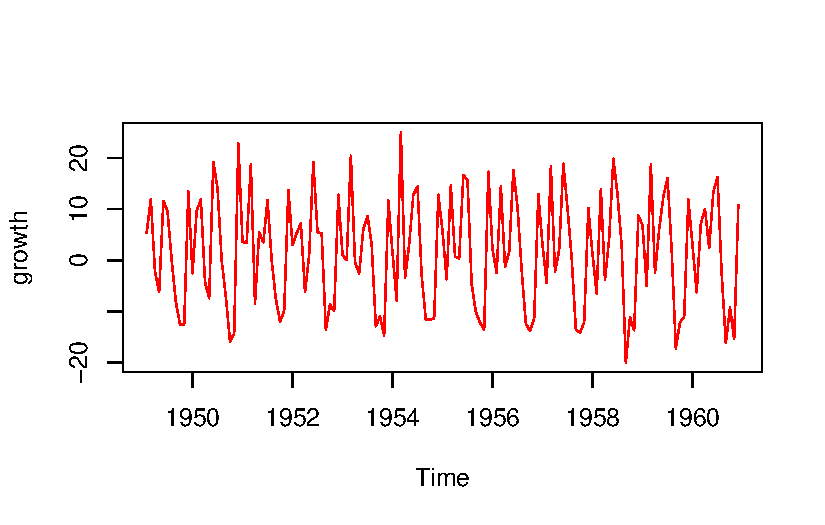
\includegraphics[keepaspectratio]{data_analysis_files/figure-pdf/unnamed-chunk-5-8.pdf}}

\section*{Veri Analizi Bazı
Paketler}\label{veri-analizi-bazux131-paketler}
\addcontentsline{toc}{section}{Veri Analizi Bazı Paketler}

\markright{Veri Analizi Bazı Paketler}

Veri analizi için
\href{https://cran.r-project.org/web/packages/skimr/vignettes/skimr.html}{skimr}
paketi de kullanılabilir. \textbf{\texttt{skimr}}, R programlama dilinde
veri setlerinin hızlı bir şekilde özetlenmesini sağlayan bir pakettir.
Veri setlerinin yapısını, özelliklerini ve bazı istatistiksel özetlerini
görsel ve açıklayıcı bir şekilde sunar. Bu paket, veri keşfi aşamasında
veri setinin genel özelliklerini anlamak için kullanılır.

\textbf{\texttt{skimr}} paketi, veri setinizdeki değişkenlerin türlerine
göre istatistiksel özetler sunar. Örneğin, sayısal değişkenler için
merkezi eğilim ölçüleri (ortalama, medyan), dağılım (standart sapma,
min-max değerleri), faktör değişkenleri için sınıf sayısı, en sık
rastlanan sınıf ve eksik veri durumları gibi bilgileri sunar.

Bu paket, veri setinin yapısını hızlıca anlamak ve önemli özelliklerini
keşfetmek için kullanılır. Özellikle veri setlerinin keşfedilmesi,
temizlenmesi ve analiz edilmesi aşamalarında oldukça faydalıdır. Bu,
veri analiz sürecinde veriye daha derinlemesine bakmayı ve hangi analiz
tekniklerinin kullanılacağına dair daha iyi bir anlayış geliştirmeyi
sağlar.

Bunun yanında, \href{https://modelsummary.com/}{modelsummary} paketi de,
R programlama dili için geliştirilmiş olan bir pakettir ve istatistiksel
modellerin özetlenmesi, karşılaştırılması ve görselleştirilmesi için
kullanılır. Bu paket, farklı türdeki modellerin çıktılarını
standartlaştırarak, bunları karşılaştırmak ve analiz etmek için
kullanıcıya kolaylık sağlar.

Bu paket genellikle doğrusal regresyon, lojistik regresyon, karar
ağaçları, destek vektör makineleri gibi çeşitli istatistiksel ve makine
öğrenimi modellerinin özet istatistiklerini, katsayılarını, belirlilik
ölçülerini, hata ölçümlerini ve diğer önemli çıktıları sunar. Bunların
yanı sıra, çıktıları tablolar halinde gösterir ve görselleştirmeler
yaparak model performansını karşılaştırmak için grafikler oluşturabilir.

Bu paket, araştırmacılar, veri bilimcileri veya istatistikçilerin farklı
modelleri anlamak, karşılaştırmak ve raporlamak için verimli bir araç
sunar. Model sonuçlarını görselleştirme ve karşılaştırma açısından
kullanışlıdır. Paket, model özetlerinin ötesinde, veri kümesine genel
bakış, korelasyon matrisleri, (çok seviyeli) çapraz tablolar ve denge
tabloları gibi son derece esnek veri özet tabloları üretmek için bir
dizi araç da içerir.

\begin{Shaded}
\begin{Highlighting}[]
\CommentTok{\# Paketin birkaç özelliğine bakalım}

\FunctionTok{library}\NormalTok{(modelsummary)}

\CommentTok{\# kategorik verilere hızlı bir bakış}
\FunctionTok{datasummary\_skim}\NormalTok{(mpg, }\StringTok{"categorical"}\NormalTok{)}
\end{Highlighting}
\end{Shaded}

\begin{table}
\centering
\begin{tabular}[t]{llrr}
\toprule
  &    & N & \%\\
\midrule
manufacturer & audi & 18 & \num{7.7}\\
 & chevrolet & 19 & \num{8.1}\\
 & dodge & 37 & \num{15.8}\\
 & ford & 25 & \num{10.7}\\
 & honda & 9 & \num{3.8}\\
 & hyundai & 14 & \num{6.0}\\
 & jeep & 8 & \num{3.4}\\
 & land rover & 4 & \num{1.7}\\
 & lincoln & 3 & \num{1.3}\\
 & mercury & 4 & \num{1.7}\\
 & nissan & 13 & \num{5.6}\\
 & pontiac & 5 & \num{2.1}\\
 & subaru & 14 & \num{6.0}\\
 & toyota & 34 & \num{14.5}\\
 & volkswagen & 27 & \num{11.5}\\
model & 4runner 4wd & 6 & \num{2.6}\\
 & a4 & 7 & \num{3.0}\\
 & a4 quattro & 8 & \num{3.4}\\
 & a6 quattro & 3 & \num{1.3}\\
 & altima & 6 & \num{2.6}\\
 & c1500 suburban 2wd & 5 & \num{2.1}\\
 & camry & 7 & \num{3.0}\\
 & camry solara & 7 & \num{3.0}\\
 & caravan 2wd & 11 & \num{4.7}\\
 & civic & 9 & \num{3.8}\\
 & corolla & 5 & \num{2.1}\\
 & corvette & 5 & \num{2.1}\\
 & dakota pickup 4wd & 9 & \num{3.8}\\
 & durango 4wd & 7 & \num{3.0}\\
 & expedition 2wd & 3 & \num{1.3}\\
 & explorer 4wd & 6 & \num{2.6}\\
 & f150 pickup 4wd & 7 & \num{3.0}\\
 & forester awd & 6 & \num{2.6}\\
 & grand cherokee 4wd & 8 & \num{3.4}\\
 & grand prix & 5 & \num{2.1}\\
 & gti & 5 & \num{2.1}\\
 & impreza awd & 8 & \num{3.4}\\
 & jetta & 9 & \num{3.8}\\
 & k1500 tahoe 4wd & 4 & \num{1.7}\\
 & land cruiser wagon 4wd & 2 & \num{0.9}\\
 & malibu & 5 & \num{2.1}\\
 & maxima & 3 & \num{1.3}\\
 & mountaineer 4wd & 4 & \num{1.7}\\
 & mustang & 9 & \num{3.8}\\
 & navigator 2wd & 3 & \num{1.3}\\
 & new beetle & 6 & \num{2.6}\\
 & passat & 7 & \num{3.0}\\
 & pathfinder 4wd & 4 & \num{1.7}\\
 & ram 1500 pickup 4wd & 10 & \num{4.3}\\
 & range rover & 4 & \num{1.7}\\
 & sonata & 7 & \num{3.0}\\
 & tiburon & 7 & \num{3.0}\\
 & toyota tacoma 4wd & 7 & \num{3.0}\\
trans & auto(av) & 5 & \num{2.1}\\
 & auto(l3) & 2 & \num{0.9}\\
 & auto(l4) & 83 & \num{35.5}\\
 & auto(l5) & 39 & \num{16.7}\\
 & auto(l6) & 6 & \num{2.6}\\
 & auto(s4) & 3 & \num{1.3}\\
 & auto(s5) & 3 & \num{1.3}\\
 & auto(s6) & 16 & \num{6.8}\\
 & manual(m5) & 58 & \num{24.8}\\
 & manual(m6) & 19 & \num{8.1}\\
drv & 4 & 103 & \num{44.0}\\
 & f & 106 & \num{45.3}\\
 & r & 25 & \num{10.7}\\
fl & c & 1 & \num{0.4}\\
 & d & 5 & \num{2.1}\\
 & e & 8 & \num{3.4}\\
 & p & 52 & \num{22.2}\\
 & r & 168 & \num{71.8}\\
class & 2seater & 5 & \num{2.1}\\
 & compact & 47 & \num{20.1}\\
 & midsize & 41 & \num{17.5}\\
 & minivan & 11 & \num{4.7}\\
 & pickup & 33 & \num{14.1}\\
 & subcompact & 35 & \num{15.0}\\
 & suv & 62 & \num{26.5}\\
\bottomrule
\end{tabular}
\end{table}

\begin{Shaded}
\begin{Highlighting}[]
\CommentTok{\# nümerik verilere hızlı bir bakış}
\FunctionTok{datasummary\_skim}\NormalTok{(mpg, }\StringTok{"numeric"}\NormalTok{)}
\end{Highlighting}
\end{Shaded}

\begin{table}
\centering
\begin{tabular}[t]{lrrrrrrr>{}r}
\toprule
  & Unique (\#) & Missing (\%) & Mean & SD & Min & Median & Max &   \\
\midrule
displ & 35 & 0 & \num{3.5} & \num{1.3} & \num{1.6} & \num{3.3} & \num{7.0} & 
\includegraphics[width=0.67in, height=0.17in]{D:/Akademi ve Veri Bilimi/Data Science/Github/r-book-tr/data_analysis_files/figure-latex/hist_4eb821f85a71.pdf}\\
year & 2 & 0 & \num{2003.5} & \num{4.5} & \num{1999.0} & \num{2003.5} & \num{2008.0} & 
\includegraphics[width=0.67in, height=0.17in]{D:/Akademi ve Veri Bilimi/Data Science/Github/r-book-tr/data_analysis_files/figure-latex/hist_4eb8af93f26.pdf}\\
cyl & 4 & 0 & \num{5.9} & \num{1.6} & \num{4.0} & \num{6.0} & \num{8.0} & 
\includegraphics[width=0.67in, height=0.17in]{D:/Akademi ve Veri Bilimi/Data Science/Github/r-book-tr/data_analysis_files/figure-latex/hist_4eb853eaaba.pdf}\\
cty & 21 & 0 & \num{16.9} & \num{4.3} & \num{9.0} & \num{17.0} & \num{35.0} & 
\includegraphics[width=0.67in, height=0.17in]{D:/Akademi ve Veri Bilimi/Data Science/Github/r-book-tr/data_analysis_files/figure-latex/hist_4eb81ebc7d64.pdf}\\
hwy & 27 & 0 & \num{23.4} & \num{6.0} & \num{12.0} & \num{24.0} & \num{44.0} & 
\includegraphics[width=0.67in, height=0.17in]{D:/Akademi ve Veri Bilimi/Data Science/Github/r-book-tr/data_analysis_files/figure-latex/hist_4eb81a59157f.pdf}\\
\bottomrule
\end{tabular}
\end{table}

\bookmarksetup{startatroot}

\chapter*{ggplot2 ile Veri
Görselleştirme}\label{ggplot2-ile-veri-guxf6rselleux15ftirme}
\addcontentsline{toc}{chapter}{ggplot2 ile Veri Görselleştirme}

\markboth{ggplot2 ile Veri Görselleştirme}{ggplot2 ile Veri
Görselleştirme}

\begin{center}

\includegraphics[width=4.4375in,height=3.20833in]{images/ggplot2.png}
\end{center}

Bu bölümde ggplot2 paketi ile verilerin nasıl görselleştirldiğine
bakacağız. ggplot2 grafiklerin dil bilgisi \textbf{(grammar of
graphics)} prensiplerini temel alarak oluşturulmuştur. Bu prensiplere
göre her grafik aynı parçalardan oluşturulabilir: bir veri seti,
koordinat sistemi, ve ``\textbf{\texttt{geom}}''lar - veri noktalarını
temsil eden görsel işaretler.

ggplot2 ile veri görselleştirebilmemiz için önce grafik yapısını iyi
tanımamız gerekiyor. Yatay eksen x ekseni, dikey eksen ise y ekseni
olarak kabul ediliyor. Veri görselleştirmede
\textbf{\texttt{ggplot}}\texttt{()} fonksiyonunu kullanıyoruz. ggplot()
fonksiyonu içinde veri seti ismi ve \textbf{\texttt{aes}}\texttt{()}
adlı estetik argümanına yatay ve dikey eksende kullanacağımız
değişkenler (sütun isimleri) ile yer veriyoruz. Sonrasında, tercih
edeceğimiz grafik tipine göre, \textbf{\texttt{geom}} fonksiyonlarından
birini kullanacağız. Sıklıkla kullanılan geom fonksiyonları şunlardır:

\begin{itemize}
\item
  Nokta grafiği için \texttt{geom\_point()}
\item
  Çubuk veya sütun grafik için \texttt{geom\_col()} ve
  \texttt{geom\_bar()}
\item
  Çizgi grafiği için \texttt{geom\_line()}
\item
  Histogram grafiği için \texttt{geom\_histogram()}
\item
  Boxplot grafiği için \texttt{geom\_boxplot()}
\end{itemize}

\section*{Dağılım Grafikleri}\label{daux11fux131lux131m-grafikleri}
\addcontentsline{toc}{section}{Dağılım Grafikleri}

\markright{Dağılım Grafikleri}

Dağılım grafikleri, veri setinin dağılımını görsel olarak temsil etmek
için kullanılan grafik türleridir. Bu grafikler, veri noktalarının,
değerlerinin veya gözlemlerinin nasıl dağıldığını incelemek ve veri
setindeki desenleri, eğilimleri ve aykırı değerleri anlamak için
kullanılır. En yaygın olanı histogram grafikleridir.

Histogram, veri setinin sayısal dağılımını gösteren bir grafiktir. Veri
aralığı belli bir aralığa bölen çubuklardan oluşur ve her çubuk, bu
aralıktaki veri noktalarının sayısını temsil eder. Histogramlar
genellikle sürekli verilerin dağılımını göstermek için kullanılır.

Bunun dışında boxplot (kutu) grafikleri de dağılımı görselleştirmek için
kullanılmaktadır. Boxplot, veri setinin beş özet istatistiği (minimum,
ilk çeyrek, medyan, üçüncü çeyrek, maksimum) kullanarak veri dağılımını
temsil eder. Bu grafik, aykırı değerleri tanımlamak ve merkezi eğilim
ile dağılımın yayılmasını görsel olarak incelemek için kullanılır.

\textbf{\texttt{geom\_histogram}} fonksiyonu, ggplot2 paketinde
kullanılan bir grafik geometrisidir ve histogram oluşturmak için
kullanılır.

\begin{Shaded}
\begin{Highlighting}[]
\FunctionTok{library}\NormalTok{(ggplot2)}
\FunctionTok{library}\NormalTok{(dplyr)}

\FunctionTok{ggplot}\NormalTok{(diamonds, }\FunctionTok{aes}\NormalTok{(price)) }\SpecialCharTok{+}
  \FunctionTok{geom\_histogram}\NormalTok{()}
\end{Highlighting}
\end{Shaded}

\pandocbounded{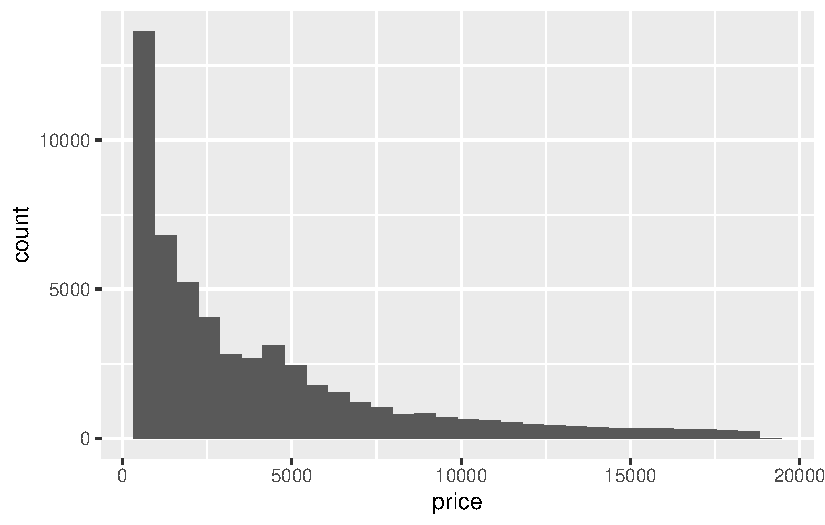
\includegraphics[keepaspectratio]{ggplot2_files/figure-pdf/unnamed-chunk-1-1.pdf}}

\textbf{\texttt{binwidth}} parametresi, histogramdaki sütunların
genişliğini (veya ``bin'' genişliğini) belirlemek için kullanılır.
Histogram, veri setini belirli aralıklara böler ve her aralıkta kaç
gözlem olduğunu gösteren sütunlardan oluşur. Bu aralıklara ``bin'' denir
ve \textbf{\texttt{binwidth}} parametresi, bu aralıkların genişliğini
belirler.

\begin{Shaded}
\begin{Highlighting}[]
\FunctionTok{ggplot}\NormalTok{(diamonds, }\FunctionTok{aes}\NormalTok{(price)) }\SpecialCharTok{+}
  \FunctionTok{geom\_histogram}\NormalTok{(}\AttributeTok{binwidth =} \DecValTok{1000}\NormalTok{,}\AttributeTok{fill =} \StringTok{"green"}\NormalTok{)}
\end{Highlighting}
\end{Shaded}

\pandocbounded{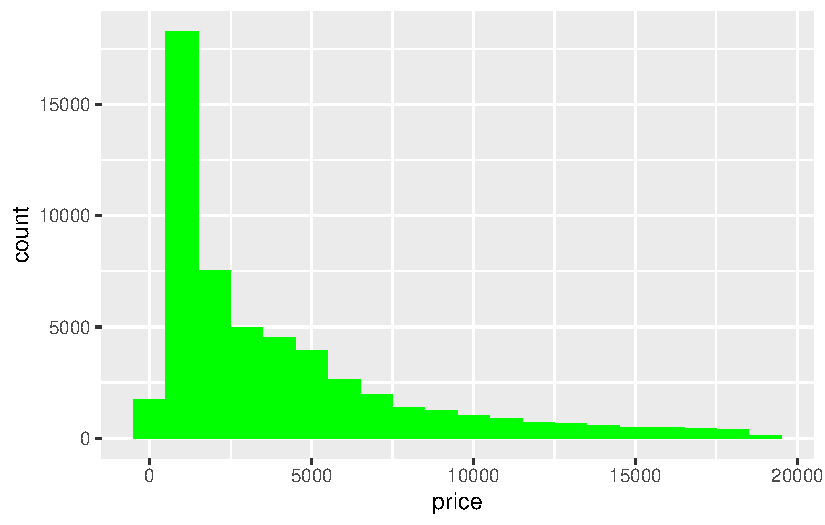
\includegraphics[keepaspectratio]{ggplot2_files/figure-pdf/unnamed-chunk-2-1.pdf}}

Bu örnekte, \textbf{\texttt{binwidth\ =\ 1000}} ifadesiyle belirtilen
bin genişliği ile bir histogram oluşturulmuştur. Bu, veri setini 1000
birim genişliğinde olan aralıklara bölecektir.

\textbf{\texttt{geom\_histogram}} fonksiyonu aynı zamanda
\textbf{\texttt{bins}} parametresini de kullanarak histogramdaki sütun
sayısını belirlemenize olanak tanır. \textbf{\texttt{bins}} parametresi,
veri setinin aralıklara bölünme sayısını belirler.

\begin{Shaded}
\begin{Highlighting}[]
\CommentTok{\# Karat değerlerinin histogramı}
\FunctionTok{ggplot}\NormalTok{(diamonds, }\FunctionTok{aes}\NormalTok{(}\AttributeTok{x =}\NormalTok{ carat)) }\SpecialCharTok{+}
  \FunctionTok{geom\_histogram}\NormalTok{(}\AttributeTok{bins =} \DecValTok{30}\NormalTok{, }\AttributeTok{fill =} \StringTok{"skyblue"}\NormalTok{, }\AttributeTok{color =} \StringTok{"black"}\NormalTok{) }\SpecialCharTok{+}
  \FunctionTok{labs}\NormalTok{(}\AttributeTok{title =} \StringTok{"Histogram of Diamond Carat"}\NormalTok{,}
       \AttributeTok{x =} \StringTok{"Carat"}\NormalTok{,}
       \AttributeTok{y =} \StringTok{"Frequency"}\NormalTok{)}
\end{Highlighting}
\end{Shaded}

\pandocbounded{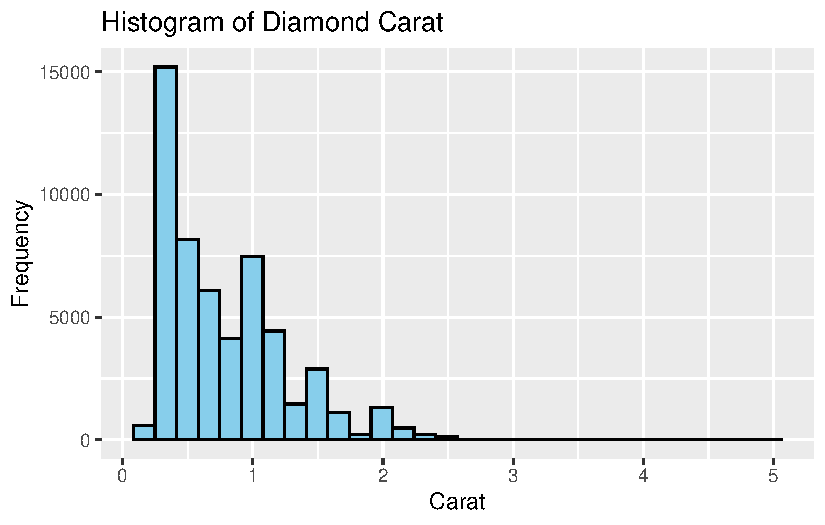
\includegraphics[keepaspectratio]{ggplot2_files/figure-pdf/unnamed-chunk-3-1.pdf}}

Bu örnekte, \textbf{\texttt{bins\ =\ 30}} ifadesiyle belirtilen 30
sütunlu bir histogram oluşturulmuştur. \textbf{\texttt{fill}} ve
\textbf{\texttt{color}} parametreleri, sütunların içinin ve kenar
çizgilerinin renklendirilmesi için kullanılmıştır.

\textbf{\texttt{alpha}} argümanı, ggplot2 paketinde kullanılan bir
estetiktir ve bir geometrinin (örneğin, nokta, çizgi, sütun, vb.)
saydamlığını kontrol etmek için kullanılır. \textbf{\texttt{alpha}}
değeri, 0 ile 1 arasında bir sayıdır; 0 tamamen şeffaflığı (görünmez) ve
1 tam opaklığı temsil eder.

Özellikle, \textbf{\texttt{alpha}} argümanı, bir nesnenin diğer
nesnelerle örtüldüğü durumları görselleştirmek için kullanışlıdır.
Örneğin, nokta, sütun veya çizgilerin birbirini örttüğü durumlarda
kullanılabilir.

\begin{Shaded}
\begin{Highlighting}[]
\CommentTok{\# Kesim sınıflarına göre karat yoğunluk fonksiyonları ile grafik oluştur}
\FunctionTok{ggplot}\NormalTok{(diamonds, }\FunctionTok{aes}\NormalTok{(}\AttributeTok{x =}\NormalTok{ carat, }\AttributeTok{fill =}\NormalTok{ cut)) }\SpecialCharTok{+}
  \FunctionTok{geom\_density}\NormalTok{(}\AttributeTok{alpha =} \FloatTok{0.5}\NormalTok{, }\AttributeTok{color =} \StringTok{"black"}\NormalTok{) }\SpecialCharTok{+}
  \FunctionTok{labs}\NormalTok{(}\AttributeTok{title =} \StringTok{"Density Plot of Carat by Cut"}\NormalTok{,}
       \AttributeTok{x =} \StringTok{"Carat"}\NormalTok{,}
       \AttributeTok{y =} \StringTok{"Density"}\NormalTok{,}
       \AttributeTok{fill =} \StringTok{"Cut"}\NormalTok{) }\SpecialCharTok{+}
  \FunctionTok{theme\_minimal}\NormalTok{()}
\end{Highlighting}
\end{Shaded}

\pandocbounded{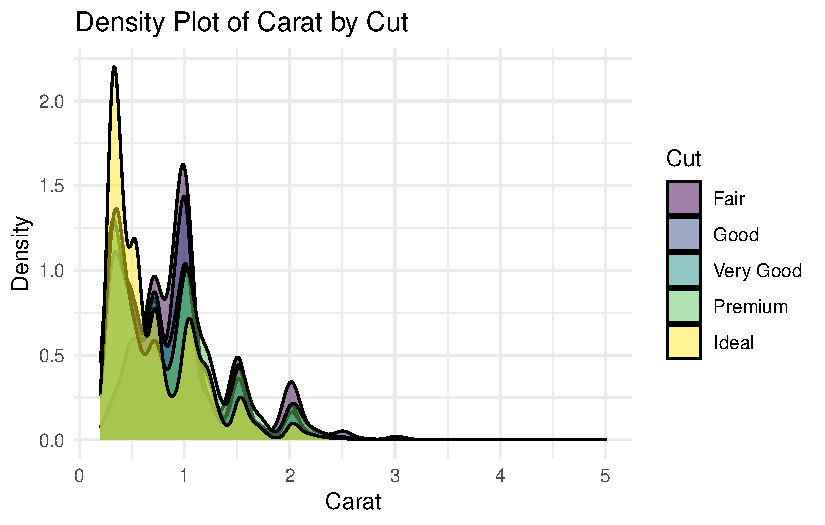
\includegraphics[keepaspectratio]{ggplot2_files/figure-pdf/unnamed-chunk-4-1.pdf}}

Bu örnekte, \textbf{\texttt{geom\_density}} fonksiyonunu kullanarak
elmasların karat değerlerinin kesim sınıflarına göre yoğunluk
fonksiyonlarını gösteren bir grafik oluşturduk.
\textbf{\texttt{alpha\ =\ 0.5}} ifadesiyle belirtilen saydamlık düzeyi,
farklı kesim sınıflarına ait yoğunluk fonksiyonlarının birbirini örttüğü
bölgeleri daha iyi görselleştirmek için kullanılmıştır.
\textbf{\texttt{color\ =\ "black"}} ifadesi ise çizgi renklerini
belirtir.

\textbf{\texttt{theme\_minimal}}, ise \textbf{\texttt{ggplot2}}
paketinde bulunan bir tema (theme) fonksiyonudur. Tema fonksiyonları,
grafiklerin görünümünü özelleştirmek için kullanılır ve çeşitli
özellikleri kontrol eder. \textbf{\texttt{theme\_minimal}} özel bir
temadır ve belirli bir stilde basitleştirilmiş bir görünüm sağlar. Bu
tema, grafik üzerindeki çizgi ve arka plan öğelerini minimalist bir
şekilde düzenler. Yani, daha az çerçeve, gölgeleme ve artı dekoratif
özellik içerir. Bu, veriyi vurgulamak ve grafiği daha okunabilir hale
getirmek amacıyla kullanılır.

\textbf{\texttt{facet\_wrap}} fonksiyonu, ggplot2 paketinde bir tema
(facet) fonksiyonudur ve veriyi belirli bir faktör veya değişkenle
bölerken, aynı grafik tasarımını korumak için kullanılır. Bu, veri
setinizin bir kategorisine göre alt grafikler oluşturmanıza olanak
tanır.

Örneğin, ``diamonds'' veri setindeki kesim sınıflarına (cut) göre karat
(carat) değerlerini gösteren bir grafik oluşturalım ve bunu
\textbf{\texttt{facet\_wrap}} kullanarak kesim sınıflarına göre ayrı alt
grafiklere bölelim.

\begin{Shaded}
\begin{Highlighting}[]
\CommentTok{\# Kesim sınıflarına göre karat değerlerini gösteren grafik oluştur}
\FunctionTok{ggplot}\NormalTok{(diamonds, }\FunctionTok{aes}\NormalTok{(}\AttributeTok{x =}\NormalTok{ carat, }\AttributeTok{fill =}\NormalTok{ cut)) }\SpecialCharTok{+}
  \FunctionTok{geom\_density}\NormalTok{(}\AttributeTok{alpha =} \FloatTok{0.5}\NormalTok{, }\AttributeTok{color =} \StringTok{"black"}\NormalTok{) }\SpecialCharTok{+}
  \FunctionTok{labs}\NormalTok{(}\AttributeTok{title =} \StringTok{"Density Plot of Carat by Cut"}\NormalTok{,}
       \AttributeTok{x =} \StringTok{"Carat"}\NormalTok{,}
       \AttributeTok{y =} \StringTok{"Density"}\NormalTok{,}
       \AttributeTok{fill =} \StringTok{"Cut"}\NormalTok{) }\SpecialCharTok{+}
  \FunctionTok{facet\_wrap}\NormalTok{(}\SpecialCharTok{\textasciitilde{}}\NormalTok{cut, }\AttributeTok{scales =} \StringTok{"free\_y"}\NormalTok{) }\SpecialCharTok{+}
  \FunctionTok{theme\_minimal}\NormalTok{()}
\end{Highlighting}
\end{Shaded}

\pandocbounded{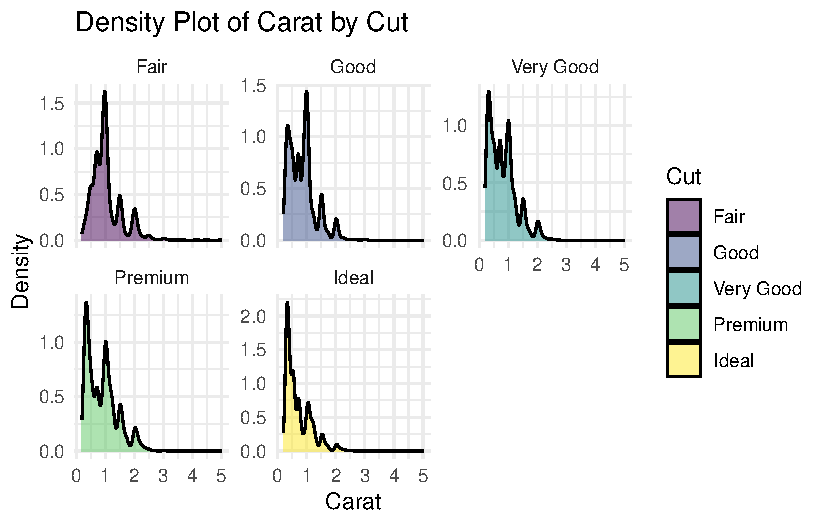
\includegraphics[keepaspectratio]{ggplot2_files/figure-pdf/unnamed-chunk-5-1.pdf}}

Bu örnekte,
\textbf{\texttt{facet\_wrap(\textasciitilde{}cut,\ scales\ =\ "free\_y")}}
ifadesi ile ``cut'' değişkenine göre alt grafiklere bölme işlemi
gerçekleştirilmiştir. \textbf{\texttt{scales\ =\ "free\_y"}} ifadesi, y
eksenlerinin serbest bırakılmasını, yani her bir alt grafikte y eksen
ölçeğinin kendi içinde adapte edilmesini sağlar. Bu, alt grafikler
arasında karşılaştırma yapmayı kolaylaştırır.

\textbf{\texttt{facet\_grid}} fonksiyonu, \textbf{\texttt{ggplot2}}
paketinde bir başka tema (facet) fonksiyonudur ve iki faktörü kullanarak
bir tabloyu alt grafiklere böler. \textbf{\texttt{facet\_wrap}}
fonksiyonu ile benzerdir, ancak farklı bir düzenleme yapısına sahiptir.
Örneğin, ``diamonds'' veri setindeki kesim sınıflarına (cut) ve renklere
(color) göre karat (carat) değerlerini gösteren bir grafik oluşturalım.

\begin{Shaded}
\begin{Highlighting}[]
\CommentTok{\# Kesim sınıflarına ve renklere göre karat değerlerini gösteren grafik oluştur}
\FunctionTok{ggplot}\NormalTok{(diamonds, }\FunctionTok{aes}\NormalTok{(}\AttributeTok{x =}\NormalTok{ carat, }\AttributeTok{fill =}\NormalTok{ cut)) }\SpecialCharTok{+}
  \FunctionTok{geom\_density}\NormalTok{(}\AttributeTok{alpha =} \FloatTok{0.5}\NormalTok{, }\AttributeTok{color =} \StringTok{"black"}\NormalTok{) }\SpecialCharTok{+}
  \FunctionTok{labs}\NormalTok{(}\AttributeTok{title =} \StringTok{"Density Plot of Carat by Cut and Color"}\NormalTok{,}
       \AttributeTok{x =} \StringTok{"Carat"}\NormalTok{,}
       \AttributeTok{y =} \StringTok{"Density"}\NormalTok{,}
       \AttributeTok{fill =} \StringTok{"Cut"}\NormalTok{) }\SpecialCharTok{+}
  \FunctionTok{facet\_grid}\NormalTok{(cut }\SpecialCharTok{\textasciitilde{}}\NormalTok{ color, }\AttributeTok{scales =} \StringTok{"free\_y"}\NormalTok{) }\SpecialCharTok{+}
  \FunctionTok{theme\_minimal}\NormalTok{()}
\end{Highlighting}
\end{Shaded}

\pandocbounded{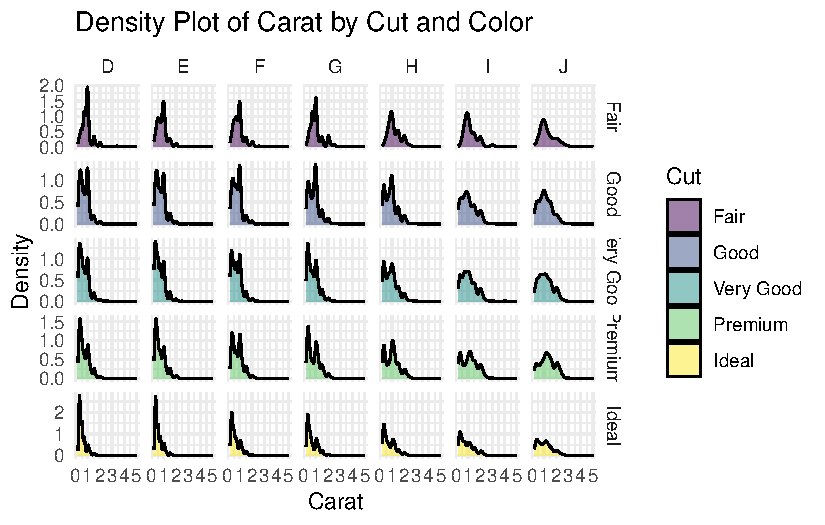
\includegraphics[keepaspectratio]{ggplot2_files/figure-pdf/unnamed-chunk-6-1.pdf}}

\textbf{\texttt{geom\_boxplot}}, ggplot2 paketinde kullanılan bir
geometri fonksiyonudur ve veri setindeki bir sayısal değişkenin
(örneğin, fiyat, karat, vb.) dağılımını görselleştirmek için kullanılır.
Bu fonksiyon, bir kutu çizgisinin çizilmesi ve altında ve üstünde yer
alan uç (whisker) hatlarıyla birlikte medyan ve çeyrekliklerin
görüntülenmesini sağlar.

Kutu grafikleri, veri dağılımının merkezi eğilimini, yayılımını ve
simetrisini hızlı bir şekilde gösteren etkili bir araçtır. Aşağıda,
``diamonds'' veri setindeki kesim sınıflarına göre fiyatların
\textbf{\texttt{geom\_boxplot}} kullanılarak nasıl görselleştirileceğine
dair bir örnek bulunmaktadır.

\begin{Shaded}
\begin{Highlighting}[]
\CommentTok{\# Kesim sınıflarına göre fiyatları gösteren boxplot oluştur}
\FunctionTok{ggplot}\NormalTok{(diamonds, }\FunctionTok{aes}\NormalTok{(}\AttributeTok{x =}\NormalTok{ cut, }\AttributeTok{y =}\NormalTok{ price, }\AttributeTok{fill =}\NormalTok{ cut)) }\SpecialCharTok{+}
  \FunctionTok{geom\_boxplot}\NormalTok{() }\SpecialCharTok{+}
  \FunctionTok{labs}\NormalTok{(}\AttributeTok{title =} \StringTok{"Boxplot of Prices by Cut"}\NormalTok{,}
       \AttributeTok{x =} \StringTok{"Cut"}\NormalTok{,}
       \AttributeTok{y =} \StringTok{"Price"}\NormalTok{,}
       \AttributeTok{fill =} \StringTok{"Cut"}\NormalTok{) }\SpecialCharTok{+}
  \FunctionTok{theme\_minimal}\NormalTok{()}
\end{Highlighting}
\end{Shaded}

\pandocbounded{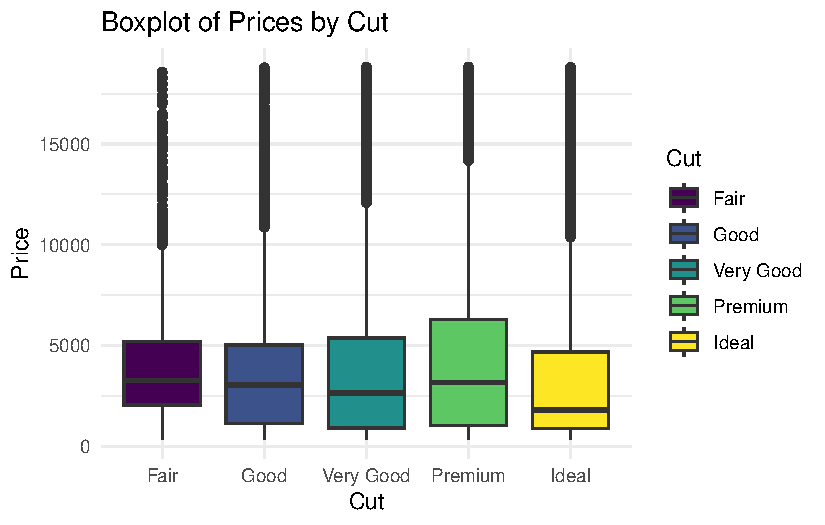
\includegraphics[keepaspectratio]{ggplot2_files/figure-pdf/unnamed-chunk-7-1.pdf}}

Bu kod, her bir kesim sınıfının fiyat dağılımını gösteren bir boxplot
oluşturur. Her bir kutu, verinin çeyrekliklerini (Q1, medyan, Q3) temsil
eder ve uç hatlar (whisker) genellikle verinin genel yayılımını
gösterir. Bu şekilde, elmas fiyatlarının kesim sınıfları arasındaki
dağılımı hızlı bir şekilde görebilirsiniz.

\textbf{\texttt{geom\_boxplot}} kullanırken ortalamayı göstermek için
bazı ek ayarlamalar yapabiliriz. Özellikle,
\textbf{\texttt{stat\_summary}} fonksiyonunu kullanarak ortalamayı
içeren bir çizgi ekleyebiliriz. Aşağıda, \textbf{\texttt{stat\_summary}}
fonksiyonunu kullanarak her kutu içindeki ortalamayı gösteren bir örnek
bulunmaktadır.

\begin{Shaded}
\begin{Highlighting}[]
\CommentTok{\# Kesim sınıflarına göre fiyatları gösteren boxplot oluştur}
\FunctionTok{ggplot}\NormalTok{(diamonds, }\FunctionTok{aes}\NormalTok{(}\AttributeTok{x =}\NormalTok{ cut, }\AttributeTok{y =}\NormalTok{ price, }\AttributeTok{fill =}\NormalTok{ cut)) }\SpecialCharTok{+}
  \FunctionTok{geom\_boxplot}\NormalTok{() }\SpecialCharTok{+}
  \FunctionTok{stat\_summary}\NormalTok{(}
    \AttributeTok{fun =}\NormalTok{ mean,}
    \AttributeTok{geom =} \StringTok{"point"}\NormalTok{,}
    \AttributeTok{shape =} \DecValTok{18}\NormalTok{,}
    \AttributeTok{size =} \DecValTok{3}\NormalTok{,}
    \AttributeTok{color =} \StringTok{"red"}\NormalTok{,}
    \AttributeTok{position =} \FunctionTok{position\_dodge}\NormalTok{(}\FloatTok{0.75}\NormalTok{)}
\NormalTok{  ) }\SpecialCharTok{+}
  \FunctionTok{labs}\NormalTok{(}\AttributeTok{title =} \StringTok{"Boxplot of Prices by Cut with Mean"}\NormalTok{,}
       \AttributeTok{x =} \StringTok{"Cut"}\NormalTok{,}
       \AttributeTok{y =} \StringTok{"Price"}\NormalTok{,}
       \AttributeTok{fill =} \StringTok{"Cut"}\NormalTok{) }\SpecialCharTok{+}
  \FunctionTok{theme\_minimal}\NormalTok{()}
\end{Highlighting}
\end{Shaded}

\pandocbounded{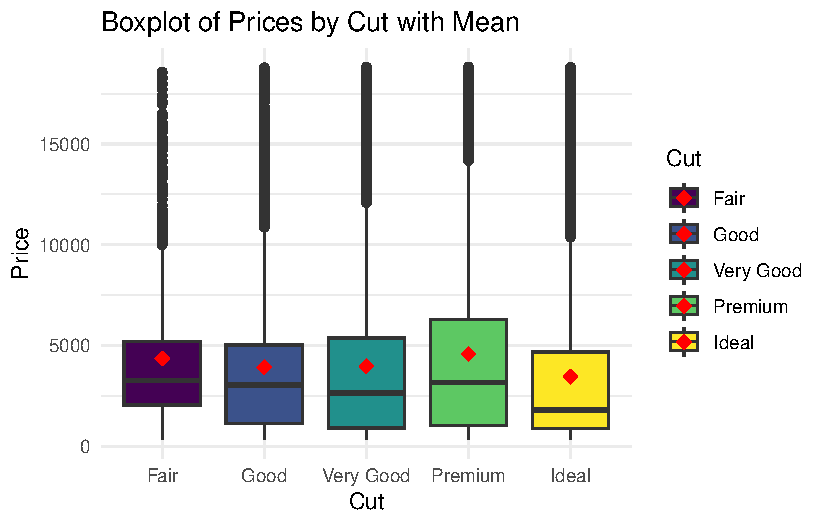
\includegraphics[keepaspectratio]{ggplot2_files/figure-pdf/unnamed-chunk-8-1.pdf}}

\textbf{\texttt{position\ =\ position\_dodge(0.75)}} ifadesi,
\textbf{\texttt{stat\_summary}} fonksiyonu içinde kullanılarak
ortalamayı temsil eden noktaların (mean points) yatay yönde bir miktar
kaydırılmasını ifade eder. Bu, ortalamayı gösteren noktaların, boxplot
içinde daha düzenli ve anlamlı bir şekilde görünmesini sağlamak için
kullanılır.

Detaylı olarak açıklamak gerekirse;
\textbf{\texttt{position\_dodge(0.75)}}, noktaların kutuların içinde
yatay yönde ne kadar kaydırılacağını belirtir. Bu değer 0 ile 1 arasında
bir sayıdır ve 0, hiç kaydırma anlamına gelirken, 1, tamamen ayrık bir
konumu temsil eder. Yani, 0.75, noktaların bir miktar sağa
kaydırılmasını ifade eder. Bu birim genellikle x-eksenindeki veri
genişliği ya da ölçeğine bağlıdır. Eğer x-eksenindeki veriler sayısal
değilse (örneğin, kategorik değişkenler) birim genişliği birimi anlam
taşımaz ve yatay konumları düzenlemede başka bir anlam ifade edebilir.
Ancak, sayısal veri genişliği olan durumlarda, bu birim genişliği
x-eksenindeki veri aralığına karşılık gelir.

\begin{tcolorbox}[enhanced jigsaw, titlerule=0mm, colbacktitle=quarto-callout-warning-color!10!white, leftrule=.75mm, colback=white, breakable, colframe=quarto-callout-warning-color-frame, bottomtitle=1mm, opacityback=0, left=2mm, title=\textcolor{quarto-callout-warning-color}{\faExclamationTriangle}\hspace{0.5em}{Dikkat}, rightrule=.15mm, opacitybacktitle=0.6, toptitle=1mm, arc=.35mm, bottomrule=.15mm, toprule=.15mm, coltitle=black]

\textbf{\texttt{position\_dodge}} fonksiyonunda belirtilen değer 1'den
büyük olabilir. Ancak, 1'den büyük bir değer kullanmak genellikle
uygunsuz sonuçlara yol açar. Bu durumda, noktalar birbirine çok yakın
hale gelir ve grafik üzerinde karışıklık olabilir. Ayarlamayı denemek ve
grafik üzerindeki etkilerini gözlemlemek, en iyi sonuca ulaşmak için
önemlidir.

\end{tcolorbox}

Bu şekilde, ortalamayı gösteren noktalar, kutular içinde daha rahat bir
şekilde görünebilir ve boxplot üzerinde daha net bir şekilde
ayrılabilir. Bu tür ayarlamalar, grafiklerin daha okunabilir ve
anlaşılır olmasına katkıda bulunabilir.

Boxplot grafiğine benzer şekilde kullanabileceğimiz başka bir grafik
çeşidi ise violin grafikleridir. Violin grafiği, bir sayısal değişkenin
dağılımını görselleştirmek için kullanılır. Violin grafiği, bir kutu
plotunun etrafına simetrik olarak yerleştirilen birer çift yay (kernel
density estimate) içerir. Bu yaylar, veri setinin yoğunluk fonksiyonunu
temsil eder ve kutu plotunun içindeki medyan, çeyreklikler ve diğer
istatistiklerle birleştirilir.

Violin grafiği, kutu plotunun sunduğu merkezi eğilim ve yayılım
bilgilerine ek olarak, veri setinin dağılımının şekli ve yoğunluğu
hakkında daha fazla bilgi sağlar. Grafiğin geniş kısımları, veri setinin
yoğun olduğu bölgeleri temsil ederken, dar kısımlar daha düşük yoğunluğa
sahip alanları gösterir. Bu sayede, violin grafiği veri setinin
dağılımının görsel bir özetini sunar.

\begin{Shaded}
\begin{Highlighting}[]
\CommentTok{\# Kesim sınıflarına göre fiyatların violin grafiği}
\FunctionTok{ggplot}\NormalTok{(diamonds, }\FunctionTok{aes}\NormalTok{(}\AttributeTok{x =}\NormalTok{ cut, }\AttributeTok{y =}\NormalTok{ price, }\AttributeTok{fill =}\NormalTok{ cut)) }\SpecialCharTok{+}
  \FunctionTok{geom\_violin}\NormalTok{() }\SpecialCharTok{+}
  \FunctionTok{labs}\NormalTok{(}\AttributeTok{title =} \StringTok{"Violin Plot of Prices by Cut"}\NormalTok{,}
       \AttributeTok{x =} \StringTok{"Cut"}\NormalTok{,}
       \AttributeTok{y =} \StringTok{"Price"}\NormalTok{,}
       \AttributeTok{fill =} \StringTok{"Cut"}\NormalTok{) }\SpecialCharTok{+}
  \FunctionTok{theme\_minimal}\NormalTok{()}
\end{Highlighting}
\end{Shaded}

\pandocbounded{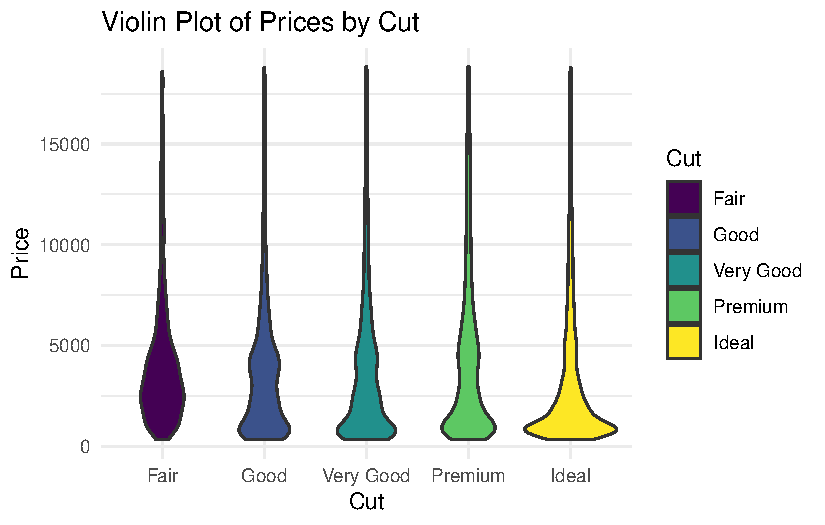
\includegraphics[keepaspectratio]{ggplot2_files/figure-pdf/unnamed-chunk-9-1.pdf}}

Bu violin grafiği, kesim sınıfları arasında fiyat dağılımlarını
karşılaştırmak için kullanılır. Violin grafiği, her bir kesim sınıfının
fiyat yoğunluğunu ve merkezi eğilimini görsel olarak özetler.

\section*{Saçılım Grafikleri}\label{sauxe7ux131lux131m-grafikleri}
\addcontentsline{toc}{section}{Saçılım Grafikleri}

\markright{Saçılım Grafikleri}

Saçılım (scatter) grafiği, genellikle fizik ve istatistik gibi
bilimlerde kullanılan bir grafik türüdür. Saçılım grafiği, iki değişken
arasındaki ilişkiyi görsel olarak göstermek için kullanılır. Bir eksende
bir değişkenin değerleri, diğer eksende ise diğer değişkenin değerleri
yer alır. Her bir nokta, veri setindeki bir gözlem birimini temsil eder.
İki değişken arasındaki ilişki, noktaların dağılımı üzerinden
anlaşılabilir.

Saçılım grafiklerinin temel amaçları şunlar:

\begin{enumerate}
\def\labelenumi{\arabic{enumi}.}
\item
  \textbf{İki Değişken Arasındaki İlişkiyi Görselleştirme:} Saçılım
  grafikleri, iki değişken arasındaki ilişkiyi anlamak için etkili bir
  araçtır. Pozitif, negatif, ya da hiçbir ilişki olup olmadığını hızlıca
  gösterir.
\item
  \textbf{Aykırı Değerleri ve Dağılımı Kontrol Etme:} Saçılım
  grafikleri, aykırı değerleri ve değişkenlerin dağılımını görsel olarak
  kontrol etmek için kullanılır.
\item
  \textbf{Korelasyon Analizi:} İki değişken arasındaki korelasyonu
  değerlendirmek için saçılım grafikleri kullanılabilir. İki değişken
  arasındaki doğrusal ilişkiyi belirlemek için korelasyon katsayısı
  kullanılabilir.
\end{enumerate}

Saçılım grafiği kullanarak, iki değişken arasındaki ilişkinin doğası
hakkında bilgi edinebilirsiniz. Örneğin, pozitif bir korelasyon varsa,
veri noktaları genellikle yukarı doğru bir eğilim gösterirken, negatif
bir korelasyon varsa, veri noktaları genellikle aşağı doğru bir eğilim
gösterir. Korelasyon olmaması durumunda ise veri noktaları dağınık bir
şekilde yayılmış olur. Saçılım grafiği, istatistiksel analizlerde veri
keşfi yapmak ve ilişkileri anlamak için önemli bir araçtır.

Şimdi, bir örnek üzerinden saçılım grafiklerini R ile nasıl
oluşturabileceğinize bakalım. Aşağıda, R'de \textbf{\texttt{mtcars}}
veri seti üzerinden bir örnek bulunmaktadır.

\begin{Shaded}
\begin{Highlighting}[]
\CommentTok{\# Saçılım grafiği oluşturma}
\FunctionTok{ggplot}\NormalTok{(mtcars, }\FunctionTok{aes}\NormalTok{(}\AttributeTok{x =}\NormalTok{ wt, }\AttributeTok{y =}\NormalTok{ mpg)) }\SpecialCharTok{+}
  \FunctionTok{geom\_point}\NormalTok{() }\SpecialCharTok{+}
  \FunctionTok{labs}\NormalTok{(}\AttributeTok{title =} \StringTok{"Saçılım Grafiği"}\NormalTok{,}
       \AttributeTok{x =} \StringTok{"Ağırlık (wt)"}\NormalTok{,}
       \AttributeTok{y =} \StringTok{"Miles Per Gallon (mpg)"}\NormalTok{)}
\end{Highlighting}
\end{Shaded}

\pandocbounded{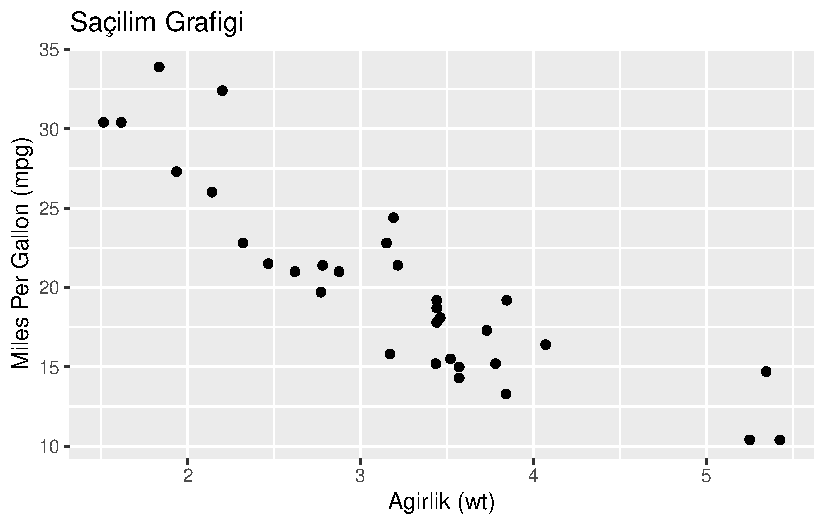
\includegraphics[keepaspectratio]{ggplot2_files/figure-pdf/unnamed-chunk-10-1.pdf}}

Bu örnekte, \textbf{\texttt{mtcars}} veri setindeki ağırlık
(\textbf{\texttt{wt}}) ve yakıt verimliliği (\textbf{\texttt{mpg}})
değişkenleri arasındaki ilişkiyi gösteren bir saçılım grafiği
oluşturduk. \textbf{\texttt{ggplot2}} paketini kullanarak
\textbf{\texttt{ggplot}} fonksiyonu ile grafiği oluşturduk, ardından
\textbf{\texttt{geom\_point()}} fonksiyonu ile noktaları ekledik ve
\textbf{\texttt{labs()}} fonksiyonu ile ekseni etiketledik.

Aşağıdaki örnek, çeşitli argümanların nasıl kullanılabileceğini
göstermektedir. Saçılım grafiklerinde kullanılabilen birçok farklı
argüman vardır ve ihtiyacınıza göre bunları özelleştirebilirsiniz. Bu
argümanlar, grafikteki renkler, şekiller, boyutlar, saydamlıklar ve
diğer estetik özellikleri kontrol etmenize olanak tanır.

\begin{Shaded}
\begin{Highlighting}[]
\CommentTok{\# Saçılım grafiği oluşturma ve özellikleri belirleme}
\FunctionTok{ggplot}\NormalTok{(mtcars, }\FunctionTok{aes}\NormalTok{(}\AttributeTok{x =}\NormalTok{ wt, }\AttributeTok{y =}\NormalTok{ mpg, }\AttributeTok{color =} \FunctionTok{factor}\NormalTok{(cyl), }\AttributeTok{size =}\NormalTok{ hp)) }\SpecialCharTok{+}
  \FunctionTok{geom\_point}\NormalTok{(}\AttributeTok{shape =} \DecValTok{16}\NormalTok{, }\AttributeTok{alpha =} \FloatTok{0.7}\NormalTok{) }\SpecialCharTok{+}  \CommentTok{\# Nokta şekli ve saydamlık}
  \FunctionTok{labs}\NormalTok{(}\AttributeTok{title =} \StringTok{"Saçılım Grafiği"}\NormalTok{,}
       \AttributeTok{x =} \StringTok{"Ağırlık (wt)"}\NormalTok{,}
       \AttributeTok{y =} \StringTok{"Miles Per Gallon (mpg)"}\NormalTok{,}
       \AttributeTok{color =} \StringTok{"Silindir Sayısı"}\NormalTok{,}
       \AttributeTok{size =} \StringTok{"Güç (hp)"}\NormalTok{) }\SpecialCharTok{+}
  \FunctionTok{theme\_minimal}\NormalTok{() }\SpecialCharTok{+}  \CommentTok{\# Tema seçimi}
  \FunctionTok{scale\_color\_manual}\NormalTok{(}\AttributeTok{values =} \FunctionTok{c}\NormalTok{(}\StringTok{"red"}\NormalTok{, }\StringTok{"green"}\NormalTok{, }\StringTok{"blue"}\NormalTok{))  }\CommentTok{\# Renk paleti}
\end{Highlighting}
\end{Shaded}

\pandocbounded{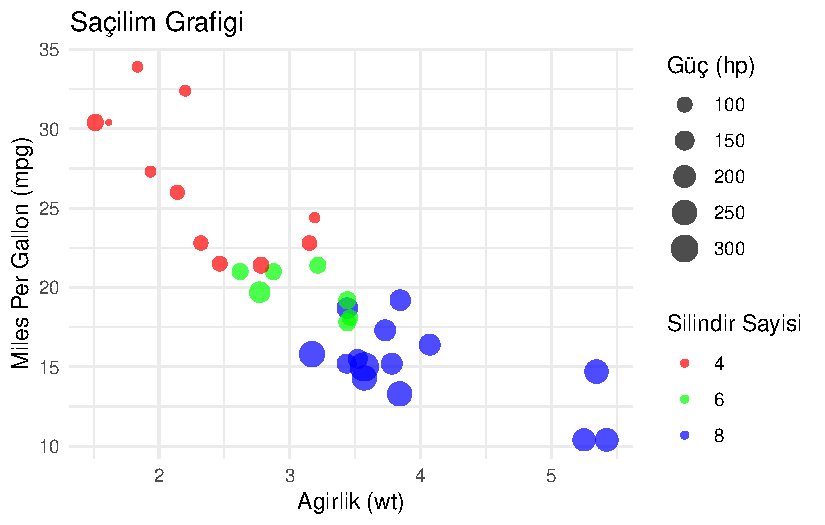
\includegraphics[keepaspectratio]{ggplot2_files/figure-pdf/unnamed-chunk-11-1.pdf}}

\begin{itemize}
\item
  \textbf{\texttt{color}}: \textbf{\texttt{factor(cyl)}} ile silindir
  sayısına göre renklendirme.
\item
  \textbf{\texttt{size}}: \textbf{\texttt{hp}} ile güç değerine göre
  nokta boyutu.
\item
  \textbf{\texttt{shape}}: \textbf{\texttt{16}} ile nokta şekli
  belirleme.
\item
  \textbf{\texttt{alpha}}: \textbf{\texttt{0.7}} ile nokta saydamlığı.
\item
  \textbf{\texttt{labs()}}: Grafik başlığı ve ekseni etiketleri.
\item
  \textbf{\texttt{theme\_minimal()}}: Minimal bir tema seçimi.
\item
  \textbf{\texttt{scale\_color\_manual()}}: Renk paletinin manuel olarak
  belirlenmesi.
\end{itemize}

\textbf{\texttt{geom\_smooth()}}, \textbf{\texttt{ggplot2}} paketinde
bulunan bir geometrik fonksiyondur ve saçılım grafiklerine regresyon
çizgisi veya düzeltme çizgisi eklemek için kullanılır. Bu fonksiyon,
veri üzerinde düzenli bir eğilimi görselleştirmek veya iki değişken
arasındaki ilişkiyi özetlemek amacıyla kullanılır.

\textbf{\texttt{geom\_smooth()}} fonksiyonu, özellikle saçılım
grafiklerindeki noktalar arasındaki eğilimi ifade etmek ve bu eğilimi
göstermek için kullanılır. Bu çizgi, genellikle loess düzeltme çizgisi
veya lineer regresyon çizgisi gibi yöntemlere dayanabilir.

\begin{tcolorbox}[enhanced jigsaw, titlerule=0mm, colbacktitle=quarto-callout-note-color!10!white, leftrule=.75mm, colback=white, breakable, colframe=quarto-callout-note-color-frame, bottomtitle=1mm, opacityback=0, left=2mm, title=\textcolor{quarto-callout-note-color}{\faInfo}\hspace{0.5em}{Loess Hakkında}, rightrule=.15mm, opacitybacktitle=0.6, toptitle=1mm, arc=.35mm, bottomrule=.15mm, toprule=.15mm, coltitle=black]

LOESS (LOcally WEighted Scatterplot Smoother), bir veri setindeki
noktalar arasındaki düzenliği ifade etmek için kullanılan bir regresyon
yöntemidir. LOESS, birçok noktadan oluşan bir saçılım grafiğine
uygulandığında, bu grafiği daha yumuşak bir eğriyle düzeltir ve genel
bir eğilimi ifade eder.

LOESS yöntemi, her bir noktanın çevresindeki komşu noktalara daha fazla
ağırlık verir ve bu ağırlıkları kullanarak her bir noktanın regresyonunu
hesaplar. Böylece, LOESS yöntemi, veri setindeki lokal düzenlemeleri
daha iyi yakalayabilir ve genel eğilimi daha esnek bir şekilde ifade
edebilir.

\end{tcolorbox}

Aşağıda, \textbf{\texttt{geom\_smooth()}} fonksiyonu ile
\textbf{\texttt{mtcars}} veri seti üzerinde bir örnek bulunmaktadır:

\begin{Shaded}
\begin{Highlighting}[]
\CommentTok{\# Saçılım grafiği oluşturma ve düzeltme çizgisi ekleme}
\FunctionTok{ggplot}\NormalTok{(mtcars, }\FunctionTok{aes}\NormalTok{(}\AttributeTok{x =}\NormalTok{ wt, }\AttributeTok{y =}\NormalTok{ mpg)) }\SpecialCharTok{+}
  \FunctionTok{geom\_point}\NormalTok{() }\SpecialCharTok{+}
  \FunctionTok{geom\_smooth}\NormalTok{(}\AttributeTok{method =} \StringTok{"lm"}\NormalTok{, }\AttributeTok{se =} \ConstantTok{FALSE}\NormalTok{, }\AttributeTok{color =} \StringTok{"blue"}\NormalTok{) }\SpecialCharTok{+}
  \FunctionTok{labs}\NormalTok{(}\AttributeTok{title =} \StringTok{"Saçılım Grafiği with Düzeltme Çizgisi"}\NormalTok{,}
       \AttributeTok{x =} \StringTok{"Ağırlık (wt)"}\NormalTok{,}
       \AttributeTok{y =} \StringTok{"Miles Per Gallon (mpg)"}\NormalTok{)}
\end{Highlighting}
\end{Shaded}

\begin{verbatim}
`geom_smooth()` using formula = 'y ~ x'
\end{verbatim}

\pandocbounded{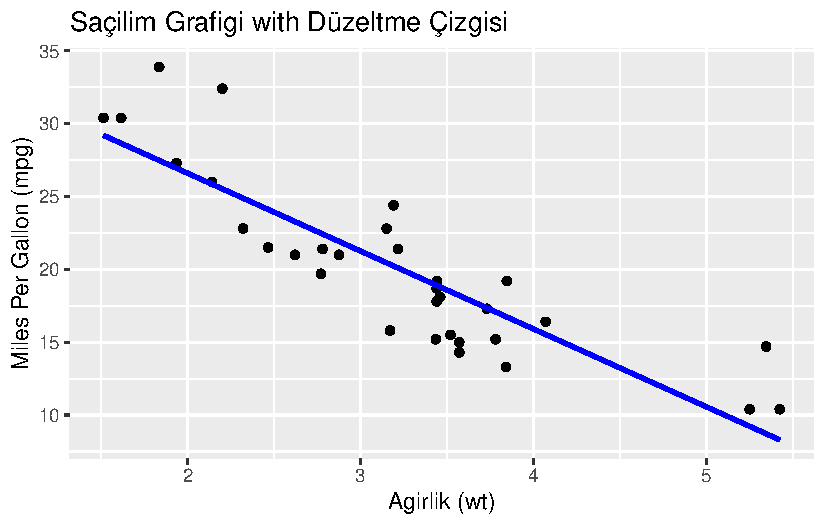
\includegraphics[keepaspectratio]{ggplot2_files/figure-pdf/unnamed-chunk-12-1.pdf}}

Bu örnekte:

\begin{itemize}
\item
  \textbf{\texttt{geom\_smooth()}} fonksiyonu, düzeltme çizgisini
  eklemek için kullanılmıştır.
\item
  \textbf{\texttt{method\ =\ "lm"}} parametresi, lineer regresyon
  modelini kullanmasını belirtir.
\item
  \textbf{\texttt{se\ =\ FALSE}} parametresi, güven aralığını
  göstermemesini sağlar.
\item
  \textbf{\texttt{color\ =\ "blue"}} parametresi, düzeltme çizgisinin
  rengini belirler.
\end{itemize}

Bu örnek, ağırlık (\textbf{\texttt{wt}}) ile yakıt verimliliği
(\textbf{\texttt{mpg}}) arasındaki ilişkiyi gösteren bir saçılım grafiği
oluşturur ve bu grafiğe bir lineer regresyon düzeltme çizgisi ekler. Bu
düzeltme çizgisi, iki değişken arasındaki genel eğilimi görsel olarak
özetler.

\textbf{\texttt{se=TRUE}} parametresi, \textbf{\texttt{geom\_smooth()}}
fonksiyonu kullanılarak eklenen düzeltme çizgisi veya eğilim çizgisi
etrafında güven aralığı (confidence interval) göstermek için kullanılır.
Güven aralığı, regresyon çizgisinin tahmini değeri etrafında belirli bir
güven düzeyindeki belirsizliği ifade eder.

Aşağıda, \textbf{\texttt{se=TRUE}} parametresi ile
\textbf{\texttt{geom\_smooth()}} kullanarak bir örnek bulunmaktadır:

\begin{Shaded}
\begin{Highlighting}[]
\CommentTok{\# Saçılım grafiği oluşturma ve düzeltme çizgisi ile güven aralığı ekleme}
\FunctionTok{ggplot}\NormalTok{(mtcars, }\FunctionTok{aes}\NormalTok{(}\AttributeTok{x =}\NormalTok{ wt, }\AttributeTok{y =}\NormalTok{ mpg)) }\SpecialCharTok{+}
  \FunctionTok{geom\_point}\NormalTok{() }\SpecialCharTok{+}
  \FunctionTok{geom\_smooth}\NormalTok{(}\AttributeTok{method =} \StringTok{"loess"}\NormalTok{, }\AttributeTok{se =} \ConstantTok{TRUE}\NormalTok{, }\AttributeTok{color =} \StringTok{"blue"}\NormalTok{) }\SpecialCharTok{+}
  \FunctionTok{labs}\NormalTok{(}\AttributeTok{title =} \StringTok{"Saçılım Grafiği{-}LOESS Düzeltme Çizgisi ve Güven Aralığı"}\NormalTok{,}
       \AttributeTok{x =} \StringTok{"Ağırlık (wt)"}\NormalTok{,}
       \AttributeTok{y =} \StringTok{"Miles Per Gallon (mpg)"}\NormalTok{)}
\end{Highlighting}
\end{Shaded}

\begin{verbatim}
`geom_smooth()` using formula = 'y ~ x'
\end{verbatim}

\pandocbounded{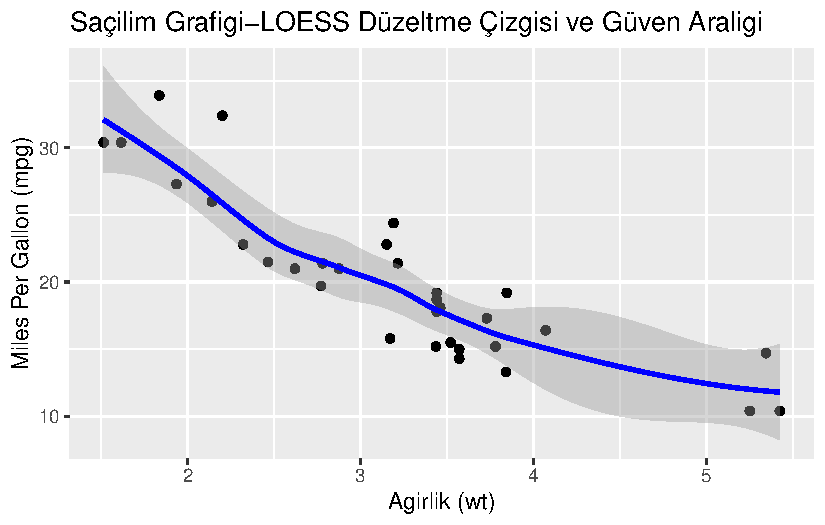
\includegraphics[keepaspectratio]{ggplot2_files/figure-pdf/unnamed-chunk-13-1.pdf}}

\begin{itemize}
\item
  \textbf{\texttt{geom\_smooth(method\ =\ "loess",\ se\ =\ TRUE,\ color\ =\ "blue")}}
  satırı, LOESS düzeltme çizgisini eklerken aynı zamanda güven aralığını
  da gösterir.
\item
  \textbf{\texttt{se\ =\ TRUE}} parametresi, güven aralığını
  etkinleştirir.
\item
  \textbf{\texttt{color\ =\ "blue"}} parametresi, çizginin rengini
  belirler.
\end{itemize}

Bu örnek grafiğin sağ tarafında çizilen mavi bant, LOESS düzeltme
çizgisinin etrafında \%95 güven aralığını temsil eder. Yani, her x
değeri için bu bant içinde düzeltilmiş tahmini değerlerin olasılığı
\%95'tir. Güven aralığı, regresyon çizgisinin ne kadar güvenilir
olduğunu ve tahminlerin belirli bir güven düzeyinde ne kadar kesin
olduğunu anlamak için kullanılır.

\section*{Sütun Grafikleri}\label{suxfctun-grafikleri}
\addcontentsline{toc}{section}{Sütun Grafikleri}

\markright{Sütun Grafikleri}

Sütun grafikleri, verileri kategorik veya gruplara göre temsil etmek
için kullanılan bir grafik türüdür. Bu grafik türü, farklı kategorilerin
veya grupların sayısal değerlerini karşılaştırmak veya görselleştirmek
için kullanılır. Sütun grafikleri dikey çubuklardan oluşur ve her çubuk,
bir kategori veya grup için bir değeri temsil eder. Sütun grafiklerinin
temel bileşenleri şunlardır:

\begin{enumerate}
\def\labelenumi{\arabic{enumi}.}
\item
  \textbf{Yatay Eksen (X-Eksen):} Bu eksende kategoriler veya gruplar
  yer alır. Örneğin, bir yıl boyunca aylar, ürün kategorileri, bölgeler
  veya şirket departmanları gibi farklı kategoriler olabilir.
\item
  \textbf{Dikey Eksen (Y-Eksen):} Bu eksende sayısal değerler yer alır
  ve sütunların yükseklikleri bu değerleri temsil eder. Değerler
  genellikle sayısal verilerdir ve karşılaştırılabilir bir ölçü birimi
  içinde bulunurlar.
\item
  \textbf{Sütunlar:} Sütunlar, her bir kategori veya grup için bir
  değeri temsil eder. Sütunların yükseklikleri, karşılaştırılan
  değerlerin büyüklüğünü veya ilişkilerini gösterir.
\end{enumerate}

Sütun grafikleri, aşağıdaki amaçlar için kullanılır:

\begin{itemize}
\item
  Karşılaştırmalar: Farklı kategorilerin veya grupların değerlerini
  karşılaştırmak için kullanılır. Örneğin, farklı ülkelerin gayri safi
  yurtiçi hasıla (GSYİH) değerlerini karşılaştırmak için sütun
  grafikleri kullanılabilir.
\item
  Zaman İçi Değişim: Zaman serisi verilerini temsil etmek için
  kullanılabilir. Her sütun, belirli bir zaman dilimindeki değerleri
  gösterebilir.
\item
  Kategorik Verilerin İncelenmesi: Ürün kategorileri, şirket
  departmanları veya müşteri segmentleri gibi kategorik verilerin
  analizi için kullanılabilir.
\end{itemize}

Sütun grafikleri, verileri görsel olarak anlamak ve veriler arasındaki
farkları veya eğilimleri vurgulamak için etkili bir araçtır. Aynı
zamanda verilerin daha kolay anlaşılmasına yardımcı olabilir ve karar
verme süreçlerine katkı sağlayabilir.

Örnekler ggplot2 paketi ile birlikte gelen
\href{https://ggplot2.tidyverse.org/reference/diamonds.html}{\textbf{\texttt{diamonds}}}
veri seti ile yapılacaktır. Veri hakkında bilgi sahibi olmak için
\textbf{\texttt{dplyr}} paketinde yer alan \textbf{\texttt{glimpse}}
fonksiyonunu kullanabiliriz. Bu fonksiyon, bir veri çerçevesi veya
tibble nesnesini özetleyen ve hızlı bir bakış sunan bir fonksiyondur.
\textbf{\texttt{glimpse}} fonksiyonu, veri setindeki değişkenleri, veri
türlerini, ve ilk birkaç gözlemi görüntüler. Ayrıca
\textbf{\texttt{summary}} fonksiyonu ile de veride yer alan
değişkenlerin temel istatistikleri hakkında bilgi sahibi olabiliriz.

\begin{Shaded}
\begin{Highlighting}[]
\FunctionTok{glimpse}\NormalTok{(diamonds)}
\end{Highlighting}
\end{Shaded}

\begin{verbatim}
Rows: 53,940
Columns: 10
$ carat   <dbl> 0.23, 0.21, 0.23, 0.29, 0.31, 0.24, 0.24, 0.26, 0.22, 0.23, 0.~
$ cut     <ord> Ideal, Premium, Good, Premium, Good, Very Good, Very Good, Ver~
$ color   <ord> E, E, E, I, J, J, I, H, E, H, J, J, F, J, E, E, I, J, J, J, I,~
$ clarity <ord> SI2, SI1, VS1, VS2, SI2, VVS2, VVS1, SI1, VS2, VS1, SI1, VS1, ~
$ depth   <dbl> 61.5, 59.8, 56.9, 62.4, 63.3, 62.8, 62.3, 61.9, 65.1, 59.4, 64~
$ table   <dbl> 55, 61, 65, 58, 58, 57, 57, 55, 61, 61, 55, 56, 61, 54, 62, 58~
$ price   <int> 326, 326, 327, 334, 335, 336, 336, 337, 337, 338, 339, 340, 34~
$ x       <dbl> 3.95, 3.89, 4.05, 4.20, 4.34, 3.94, 3.95, 4.07, 3.87, 4.00, 4.~
$ y       <dbl> 3.98, 3.84, 4.07, 4.23, 4.35, 3.96, 3.98, 4.11, 3.78, 4.05, 4.~
$ z       <dbl> 2.43, 2.31, 2.31, 2.63, 2.75, 2.48, 2.47, 2.53, 2.49, 2.39, 2.~
\end{verbatim}

\begin{Shaded}
\begin{Highlighting}[]
\FunctionTok{summary}\NormalTok{(diamonds)}
\end{Highlighting}
\end{Shaded}

\begin{verbatim}
     carat               cut        color        clarity          depth      
 Min.   :0.2000   Fair     : 1610   D: 6775   SI1    :13065   Min.   :43.00  
 1st Qu.:0.4000   Good     : 4906   E: 9797   VS2    :12258   1st Qu.:61.00  
 Median :0.7000   Very Good:12082   F: 9542   SI2    : 9194   Median :61.80  
 Mean   :0.7979   Premium  :13791   G:11292   VS1    : 8171   Mean   :61.75  
 3rd Qu.:1.0400   Ideal    :21551   H: 8304   VVS2   : 5066   3rd Qu.:62.50  
 Max.   :5.0100                     I: 5422   VVS1   : 3655   Max.   :79.00  
                                    J: 2808   (Other): 2531                  
     table           price             x                y         
 Min.   :43.00   Min.   :  326   Min.   : 0.000   Min.   : 0.000  
 1st Qu.:56.00   1st Qu.:  950   1st Qu.: 4.710   1st Qu.: 4.720  
 Median :57.00   Median : 2401   Median : 5.700   Median : 5.710  
 Mean   :57.46   Mean   : 3933   Mean   : 5.731   Mean   : 5.735  
 3rd Qu.:59.00   3rd Qu.: 5324   3rd Qu.: 6.540   3rd Qu.: 6.540  
 Max.   :95.00   Max.   :18823   Max.   :10.740   Max.   :58.900  
                                                                  
       z         
 Min.   : 0.000  
 1st Qu.: 2.910  
 Median : 3.530  
 Mean   : 3.539  
 3rd Qu.: 4.040  
 Max.   :31.800  
                 
\end{verbatim}

Sütun grafiği üretebilmek için kullanılan fonksiyonlardan bir tanesi
\textbf{\texttt{geom\_bar()}}'dır. Aşağıda verilen kod veri setindeki
kesim sınıflarını ifade eden \textbf{\texttt{cut}} değişkenin
frekanslarını gösteren bir sütun grafik üretir. Her bir sütun, belirli
bir kesim sınıfını temsil eder ve yükseklikleri o kesim sınıfına ait
elmas sayısını yansıtır.

\begin{Shaded}
\begin{Highlighting}[]
\CommentTok{\# sıklık durumunu görselleştirme}
\FunctionTok{ggplot}\NormalTok{(diamonds, }\FunctionTok{aes}\NormalTok{(cut)) }\SpecialCharTok{+}
  \FunctionTok{geom\_bar}\NormalTok{()}
\end{Highlighting}
\end{Shaded}

\pandocbounded{\includegraphics[keepaspectratio]{ggplot2_files/figure-pdf/unnamed-chunk-15-1.pdf}}

Örneğin \textbf{\texttt{color}} değişkenine göre gruplandırılmış bir
grafik üretelim. Aşağıda yer alan kod, ``diamonds'' veri setindeki kesim
sınıflarının ve renklerinin kombinasyonlarına göre gruplandırılmış bir
sütun grafik üretir. Her bir \textbf{\texttt{cut}} kategorisi için ayrı
renkli sütunlar olacaktır.

\begin{itemize}
\item
  \textbf{\texttt{ggplot(diamonds,\ aes(cut,\ fill\ =\ color))}}: Bu
  bölümde, ``diamonds'' veri setini temel alarak bir ggplot nesnesi
  oluşturulur. \textbf{\texttt{aes(cut,\ fill\ =\ color)}} ifadesi, x
  ekseninde ``cut'' değişkenini, sütunların renklendirilmesinde ise
  ``color'' değişkenini kullanacağımızı belirtir.
\item
  \textbf{\texttt{geom\_bar(position\ =\ position\_dodge())}}: Bu
  fonksiyon, gruplandırılmış sütun grafik oluşturur.
  \textbf{\texttt{position\ =\ position\_dodge()}} ifadesi, sütunların
  yan yana yerleştirilmesini sağlar, yani her bir \textbf{\texttt{cut}}
  kategorisi içindeki \textbf{\texttt{color}} kategorilerini farklı
  renklerde gösterir. Bu sayede, her bir \textbf{\texttt{cut}}
  kategorisi için ayrı renkli sütunlar elde edilir.
\end{itemize}

\begin{Shaded}
\begin{Highlighting}[]
\FunctionTok{ggplot}\NormalTok{(diamonds, }\FunctionTok{aes}\NormalTok{(cut, }\AttributeTok{fill =}\NormalTok{ color)) }\SpecialCharTok{+}
  \FunctionTok{geom\_bar}\NormalTok{(}\AttributeTok{position =} \FunctionTok{position\_dodge}\NormalTok{()) }\SpecialCharTok{+} 
  \FunctionTok{xlab}\NormalTok{(}\StringTok{"Pirlanta kaliteleri"}\NormalTok{) }\SpecialCharTok{+} 
  \FunctionTok{ylab}\NormalTok{(}\StringTok{"Gozlenme Sikliklari"}\NormalTok{)}
\end{Highlighting}
\end{Shaded}

\pandocbounded{\includegraphics[keepaspectratio]{ggplot2_files/figure-pdf/unnamed-chunk-16-1.pdf}}

Her bir kesim sınıfı için, \textbf{\texttt{color}} değişkenine göre
renklendirilmiş sütunları olan ve her sütunun yüksekliği, o kesim
sınıfındaki elmasların toplam karat değerini temsil eden bir grafik
üretelim. Bu durumda y ekseninde \textbf{\texttt{carat}} değişkenini
kullanacağız.

\textbf{\texttt{geom\_bar(stat\ =\ "identity")}}: Bu fonksiyon,
gruplandırılmış sütun grafik oluşturur.
\textbf{\texttt{stat\ =\ "identity"}} ifadesi, her bir sütunun
yüksekliğinin, ``carat'' değişkeninin değerine eşit olacağını belirtir.
Yani, sütunların yüksekliği doğrudan carat değişkenine bağlı olacaktır.

\begin{Shaded}
\begin{Highlighting}[]
\FunctionTok{ggplot}\NormalTok{(diamonds, }\FunctionTok{aes}\NormalTok{(}\AttributeTok{x=}\NormalTok{cut, }\AttributeTok{y=}\NormalTok{carat,}\AttributeTok{fill =}\NormalTok{ color)) }\SpecialCharTok{+}
  \FunctionTok{geom\_bar}\NormalTok{(}\AttributeTok{stat =} \StringTok{"identity"}\NormalTok{) }
\end{Highlighting}
\end{Shaded}

\pandocbounded{\includegraphics[keepaspectratio]{ggplot2_files/figure-pdf/unnamed-chunk-17-1.pdf}}

Eğer \textbf{\texttt{position\ =\ "fill"}} kullanırsak,
\textbf{\texttt{geom\_bar}} fonksiyonu, her kategori içindeki değerlerin
oranlarını gösteren yığılmış bir sütun grafik oluşturur. Bu durumda, her
bir kategori toplam yüksekliğe göre doldurulacak ve her bir alt
kategori, kendi kategorisi içindeki oranını ifade edecek şekilde
düzenlenecektir.

\begin{Shaded}
\begin{Highlighting}[]
\FunctionTok{ggplot}\NormalTok{(diamonds, }\FunctionTok{aes}\NormalTok{(}\AttributeTok{x=}\NormalTok{cut, }\AttributeTok{y=}\NormalTok{carat,}\AttributeTok{fill =}\NormalTok{ color)) }\SpecialCharTok{+}
  \CommentTok{\# fill ile oransal olarak gösterim yapılır}
  \FunctionTok{geom\_bar}\NormalTok{(}\AttributeTok{stat =} \StringTok{"identity"}\NormalTok{,}\AttributeTok{position =} \StringTok{"fill"}\NormalTok{) }
\end{Highlighting}
\end{Shaded}

\pandocbounded{\includegraphics[keepaspectratio]{ggplot2_files/figure-pdf/unnamed-chunk-18-1.pdf}}

Her bir kesim sınıfının toplam yüksekliğe göre doldurulduğu bu grafikte,
her renk kategorisi içindeki sütunlar, o kesim sınıfındaki toplam elmas
sayısına oranlanmış şekilde görüntülenir. Bu tür bir grafik, her bir
kategorinin toplamda ne kadar paya sahip olduğunu vurgulamak ve
kategorinin içindeki alt kategorilerin oranlarını göstermek için
kullanışlıdır. Ancak, grafikteki renklerin yorumlanması dikkatlice
yapılmalıdır, çünkü her renk, kendi kategorisi içindeki oranları temsil
eder.

\begin{tcolorbox}[enhanced jigsaw, titlerule=0mm, colbacktitle=quarto-callout-warning-color!10!white, leftrule=.75mm, colback=white, breakable, colframe=quarto-callout-warning-color-frame, bottomtitle=1mm, opacityback=0, left=2mm, title=\textcolor{quarto-callout-warning-color}{\faExclamationTriangle}\hspace{0.5em}{Dikkat}, rightrule=.15mm, opacitybacktitle=0.6, toptitle=1mm, arc=.35mm, bottomrule=.15mm, toprule=.15mm, coltitle=black]

İki tür çubuk grafik vardır: \textbf{\texttt{geom\_bar()}} ve
\textbf{\texttt{geom\_col()}}. \textbf{geom\_bar()}, çubuğun
yüksekliğini her gruptaki vaka sayısıyla (veya ağırlık estetiği
sağlanmışsa, ağırlıkların toplamıyla) orantılı hale getirir. Çubukların
yüksekliklerinin verilerdeki değerleri temsil etmesini istiyorsanız,
bunun yerine \textbf{\texttt{geom\_col()}} kullanın.
\textbf{geom\_bar()} varsayılan olarak \textbf{\texttt{stat\_count()}}
kullanır: her x konumundaki vaka sayısını sayar.
\textbf{\texttt{geom\_col()}} \textbf{\texttt{stat\_identity()}}
kullanır. Yani verileri olduğu gibi bırakır.

\end{tcolorbox}

\section*{Zaman Serisi Grafikleri}\label{zaman-serisi-grafikleri}
\addcontentsline{toc}{section}{Zaman Serisi Grafikleri}

\markright{Zaman Serisi Grafikleri}

Zaman serisi grafikleri, zamanla değişen verileri görsel olarak temsil
etmek için kullanılan grafiklerdir. Bu tür grafikler, belirli bir süre
boyunca gözlemlenen verileri analiz etmek, eğilimleri belirlemek,
dönemsel desenleri tanımak ve istatistiksel analizler yapmak için yaygın
olarak kullanılır. Zaman serisi verileri genellikle sabit aralıklarla
veya farklı zaman dilimlerinde toplanır. En yaygın olan türü çizgi
grafikleri olmakla birlikte sütun ve alan grafikleri de zaman
serilerinin görselleştirilmesinde kullanılabilmektedir.

Örnekler ggplot2 paketi ile birlikte gelen
\href{https://ggplot2.tidyverse.org/reference/economics.html}{\textbf{\texttt{economics}}}
veri seti ile yapılacaktır.

\begin{Shaded}
\begin{Highlighting}[]
\CommentTok{\# verileri inceleyelim}
\NormalTok{economics}
\end{Highlighting}
\end{Shaded}

\begin{verbatim}
# A tibble: 574 x 6
   date         pce    pop psavert uempmed unemploy
   <date>     <dbl>  <dbl>   <dbl>   <dbl>    <dbl>
 1 1967-07-01  507. 198712    12.6     4.5     2944
 2 1967-08-01  510. 198911    12.6     4.7     2945
 3 1967-09-01  516. 199113    11.9     4.6     2958
 4 1967-10-01  512. 199311    12.9     4.9     3143
 5 1967-11-01  517. 199498    12.8     4.7     3066
 6 1967-12-01  525. 199657    11.8     4.8     3018
 7 1968-01-01  531. 199808    11.7     5.1     2878
 8 1968-02-01  534. 199920    12.3     4.5     3001
 9 1968-03-01  544. 200056    11.7     4.1     2877
10 1968-04-01  544  200208    12.3     4.6     2709
# i 564 more rows
\end{verbatim}

\begin{Shaded}
\begin{Highlighting}[]
\FunctionTok{summary}\NormalTok{(economics)}
\end{Highlighting}
\end{Shaded}

\begin{verbatim}
      date                 pce               pop            psavert      
 Min.   :1967-07-01   Min.   :  506.7   Min.   :198712   Min.   : 2.200  
 1st Qu.:1979-06-08   1st Qu.: 1578.3   1st Qu.:224896   1st Qu.: 6.400  
 Median :1991-05-16   Median : 3936.8   Median :253060   Median : 8.400  
 Mean   :1991-05-17   Mean   : 4820.1   Mean   :257160   Mean   : 8.567  
 3rd Qu.:2003-04-23   3rd Qu.: 7626.3   3rd Qu.:290291   3rd Qu.:11.100  
 Max.   :2015-04-01   Max.   :12193.8   Max.   :320402   Max.   :17.300  
    uempmed          unemploy    
 Min.   : 4.000   Min.   : 2685  
 1st Qu.: 6.000   1st Qu.: 6284  
 Median : 7.500   Median : 7494  
 Mean   : 8.609   Mean   : 7771  
 3rd Qu.: 9.100   3rd Qu.: 8686  
 Max.   :25.200   Max.   :15352  
\end{verbatim}

\textbf{\texttt{economics}} veri setinde bulunan \textbf{\texttt{date}}
ve \textbf{\texttt{pce}} (Personal Consumption Expenditures - Kişisel
Tüketim Harcamaları) değişkenlerini kullanarak bir zaman serisi grafiği
oluşturalım.

\begin{Shaded}
\begin{Highlighting}[]
\NormalTok{p }\OtherTok{\textless{}{-}}\NormalTok{ economics }\SpecialCharTok{\%\textgreater{}\%} 
  \FunctionTok{ggplot}\NormalTok{(}\FunctionTok{aes}\NormalTok{(}\AttributeTok{x=}\NormalTok{date,}\AttributeTok{y=}\NormalTok{pce)) }\SpecialCharTok{+}
  \FunctionTok{geom\_line}\NormalTok{(}\AttributeTok{color=}\StringTok{"blue"}\NormalTok{) }\SpecialCharTok{+}
  \FunctionTok{theme\_minimal}\NormalTok{() }\SpecialCharTok{+}
  \FunctionTok{labs}\NormalTok{(}\AttributeTok{x =} \StringTok{""}\NormalTok{,}
       \AttributeTok{y =} \StringTok{"Personal Consumption Expenditures"}\NormalTok{,}
       \AttributeTok{title =} \StringTok{"Personal Consumption Expenditures Time Series"}\NormalTok{,}
       \AttributeTok{caption =} \StringTok{"Economics Data"}\NormalTok{,}
       \AttributeTok{subtitle =} \StringTok{"Economics Data (1967{-}2015)"}\NormalTok{)}
\NormalTok{p}
\end{Highlighting}
\end{Shaded}

\pandocbounded{\includegraphics[keepaspectratio]{ggplot2_files/figure-pdf/unnamed-chunk-20-1.pdf}}

Aşağıda bu kodun adım adım açıklamasını bulabilirsiniz:

\begin{itemize}
\item
  \textbf{\texttt{economics\ \%\textgreater{}\%}}: Bu işlem, ``pipe''
  (\textbf{\texttt{\%\textgreater{}\%}}) operatörünü kullanarak
  \textbf{\texttt{economics}} veri setini bir dizi başka işleme
  yönlendirir. Bu, veri manipülasyonunu daha okunabilir ve zincirleme
  bir şekilde yapmamıza olanak tanır.
\item
  \textbf{\texttt{ggplot(aes(x=date,\ y=pce))}}:
  \textbf{\texttt{ggplot()}} fonksiyonu, temel bir grafik oluşturur.
  \textbf{\texttt{aes()}} fonksiyonu içinde \textbf{\texttt{x}} ve
  \textbf{\texttt{y}} argümanları, grafiğin x ve y eksenine hangi
  verilerin yerleştirileceğini belirtir. Bu durumda, x ekseni
  \textbf{\texttt{date}} değişkenini, y ekseni ise \textbf{\texttt{pce}}
  değişkenini kullanır.
\item
  \textbf{\texttt{geom\_line(color="blue")}}:
  \textbf{\texttt{geom\_line()}} fonksiyonu, bir çizgi grafiği ekler. Bu
  durumda, \textbf{\texttt{color="blue"}} argümanı ile çizgi rengi mavi
  olarak belirlenmiştir.
\item
  \textbf{\texttt{theme\_minimal()}}: Bu fonksiyon, grafiği daha sade
  bir görünüme getirmek için kullanılır. Başka temalar da seçilebilir.
\item
  \textbf{\texttt{labs(x="",\ y="Personal\ Consumption\ Expenditures",\ title="Personal\ Consumption\ Expenditures\ Time\ Series",\ caption="Economics\ Data",\ subtitle="Economics\ Data\ (1967-2015)")}}:
  \textbf{\texttt{labs()}} fonksiyonu, grafiğin başlığını, eksen
  etiketlerini ve diğer metin öğelerini ayarlar. \textbf{\texttt{x=""}}
  ile x ekseninin başlığı kaldırılmış,
  \textbf{\texttt{y="Personal\ Consumption\ Expenditures"}} ile y
  ekseninin başlığı belirlenmiş,
  \textbf{\texttt{title="Personal\ Consumption\ Expenditures\ Time\ Series"}}
  ile grafik başlığı belirlenmiş,
  \textbf{\texttt{subtitle="Economics\ Data\ (1967-2015)"}} ile alt
  başlık eklenmiştir.
\end{itemize}

Bu kod, \textbf{\texttt{economics}} veri setindeki tüketim
harcamalarının zaman içindeki değişimini mavi bir çizgi grafiği ile
gösteren bir ggplot2 grafiği oluşturur.

\begin{Shaded}
\begin{Highlighting}[]
\CommentTok{\# zaman eksenini ve legend ayarlama}
\NormalTok{p }\SpecialCharTok{+} 
  \FunctionTok{scale\_x\_date}\NormalTok{(}\AttributeTok{date\_breaks =} \StringTok{"1 year"}\NormalTok{, }\AttributeTok{date\_labels =} \StringTok{"\%Y"}\NormalTok{) }\SpecialCharTok{+}
  \FunctionTok{theme}\NormalTok{(}\AttributeTok{axis.text.x =} \FunctionTok{element\_text}\NormalTok{(}\AttributeTok{angle =} \DecValTok{45}\NormalTok{), }\AttributeTok{legend.position =} \StringTok{"top"}\NormalTok{)}
\end{Highlighting}
\end{Shaded}

\pandocbounded{\includegraphics[keepaspectratio]{ggplot2_files/figure-pdf/unnamed-chunk-21-1.pdf}}

\textbf{\texttt{p}} ismini verdiğimiz grafik objesine eklenen kısım,
\textbf{\texttt{scale\_x\_date()}} ve \textbf{\texttt{theme()}}
fonksiyonlarıyla grafiğin x ekseni üzerindeki tarih etiketlerini ve
genel görünümü özelleştirmektedir. Aşağıda bu kodun eklenmiş haliyle
birlikte açıklamasını bulabilirsiniz:

\begin{itemize}
\item
  \textbf{\texttt{scale\_x\_date(date\_breaks\ =\ "1\ year",\ date\_labels\ =\ "\%Y")}}:
  Bu bölüm, x ekseni üzerindeki tarih etiketlerini özelleştirmek için
  kullanılır. \textbf{\texttt{date\_breaks}} argümanı, tarih
  etiketlerinin kaç yılda bir görüneceğini belirler.
  \textbf{\texttt{date\_labels}} argümanı ise tarih etiketlerinin nasıl
  formatlanacağını belirler. Bu örnekte, her yılın gösterilmesi ve yıl
  formatında görüntülenmesi belirlenmiştir.
\item
  \textbf{\texttt{theme(axis.text.x\ =\ element\_text(angle\ =\ 45),\ legend.position\ =\ "top")}}:
  Bu bölüm, genel görünümü özelleştirmek için kullanılır.
  \textbf{\texttt{axis.text.x}} ile x ekseni etiketlerinin açısını
  belirleyebiliriz (burada 45 derece olarak belirlenmiştir).
  \textbf{\texttt{legend.position}} ile ise lejantın grafiğin neresinde
  yer alacağını belirleyebiliriz (burada ``top'' olarak belirlenmiştir).
\end{itemize}

Bu eklemelerle birlikte, grafiğin x ekseni üzerinde yıllık tarih
etiketleri görünecek ve bu etiketler 45 derece eğimli olacak. Ayrıca,
lejant grafiğin üst kısmına yerleştirilecektir.

\begin{Shaded}
\begin{Highlighting}[]
\NormalTok{p }\SpecialCharTok{+} 
  \FunctionTok{scale\_x\_date}\NormalTok{(}\AttributeTok{date\_breaks =} \StringTok{"2 year"}\NormalTok{, }\AttributeTok{date\_labels =} \StringTok{"\%Y"}\NormalTok{,}\AttributeTok{expand =} \FunctionTok{c}\NormalTok{(}\DecValTok{0}\NormalTok{,}\DecValTok{0}\NormalTok{)) }\SpecialCharTok{+}
  \FunctionTok{theme}\NormalTok{(}\AttributeTok{axis.text.x =} \FunctionTok{element\_text}\NormalTok{(}\AttributeTok{angle =} \DecValTok{45}\NormalTok{), }\AttributeTok{legend.position =} \StringTok{"top"}\NormalTok{)}
\end{Highlighting}
\end{Shaded}

\pandocbounded{\includegraphics[keepaspectratio]{ggplot2_files/figure-pdf/unnamed-chunk-22-1.pdf}}

Eklendiğiniz bu kod parçası ile x eksenindeki tarih etiketleri, 2 yılda
bir görünecek şekilde ayarlanmıştır
(\textbf{\texttt{date\_breaks\ =\ "2\ year"}}). Ayrıca,
\textbf{\texttt{expand\ =\ c(0,\ 0)}} ile x ekseninin başlangıç ve
bitişindeki boşluklar sıfır olarak belirlenmiştir. Bu, x ekseninin
kenarlarına sıfır boşluk bırakarak grafiği daha kompakt hale getirir.

\begin{Shaded}
\begin{Highlighting}[]
\CommentTok{\# çizgi türü değiştirilebilir}
\NormalTok{economics }\SpecialCharTok{\%\textgreater{}\%} 
  \FunctionTok{ggplot}\NormalTok{(}\FunctionTok{aes}\NormalTok{(}\AttributeTok{x=}\NormalTok{date,}\AttributeTok{y=}\NormalTok{pce)) }\SpecialCharTok{+}
  \FunctionTok{geom\_line}\NormalTok{(}\AttributeTok{linetype =} \StringTok{"dashed"}\NormalTok{, }\AttributeTok{size =} \DecValTok{1}\NormalTok{, }\AttributeTok{colour =} \StringTok{"blue"}\NormalTok{)}
\end{Highlighting}
\end{Shaded}

\pandocbounded{\includegraphics[keepaspectratio]{ggplot2_files/figure-pdf/unnamed-chunk-23-1.pdf}}

\textbf{\texttt{linetype}} argümanı, çizgi tipini belirler (burada
``dashed'' olarak belirlenmiştir). \textbf{\texttt{size}} argümanı,
çizgi kalınlığını belirler (1 olarak belirlenmiştir).
\textbf{\texttt{colour}} argümanı ise çizgi rengini belirler (mavi
olarak belirlenmiştir).

\begin{tcolorbox}[enhanced jigsaw, titlerule=0mm, colbacktitle=quarto-callout-tip-color!10!white, leftrule=.75mm, colback=white, breakable, colframe=quarto-callout-tip-color-frame, bottomtitle=1mm, opacityback=0, left=2mm, title=\textcolor{quarto-callout-tip-color}{\faLightbulb}\hspace{0.5em}{Ek Bilgi}, rightrule=.15mm, opacitybacktitle=0.6, toptitle=1mm, arc=.35mm, bottomrule=.15mm, toprule=.15mm, coltitle=black]

\textbf{\texttt{linetype}} parametresi, \textbf{\texttt{geom\_line()}}
fonksiyonu ile çizgi grafiği oluştururken çizgi tipini belirlemek için
kullanılır. Bu parametre, çeşitli değerleri kabul eder. İşte yaygın
olarak kullanılan bazı \textbf{\texttt{linetype}} değerleri:

\begin{enumerate}
\def\labelenumi{\arabic{enumi}.}
\item
  \textbf{\texttt{"solid"}}: Tam çizgi (Varsayılan).
\item
  \textbf{\texttt{"dashed"}}: Kesikli çizgi.
\item
  \textbf{\texttt{"dotted"}}: Noktalı çizgi.
\item
  \textbf{\texttt{"dotdash"}}: Noktalı-kesikli çizgi.
\item
  \textbf{\texttt{"longdash"}}: Uzun kesikli çizgi.
\item
  \textbf{\texttt{"twodash"}}: Çift kesikli çizgi.
\item
  \textbf{\texttt{"blank"}}: Hiç çizgi çizme (görselde görüntülenmez).
\end{enumerate}

Örneğin, \textbf{\texttt{linetype\ =\ "dashed"}} ifadesi, çizginin
kesikli olacağını belirtir. Bu değeri dışında başka özelleştirmeler de
yapabilirsiniz. \textbf{\texttt{linetype}} parametresi, daha karmaşık
çizgi tipleri oluşturmak için farklı uzunluk ve boşluk kombinasyonlarına
da izin verir.

\textbf{\texttt{linetype}} parametresine yerine sayısal değerleri de
atanabilir. Örneğin \textbf{\texttt{linetype\ =\ 1}} ifadesi
\textbf{\texttt{linetype\ =\ "solid"}} ile aynı anlama gelir. Yukarıda
verilen \textbf{\texttt{linetype}} türlerinin yanındaki da rakamlar da
kullanılabilir.

\end{tcolorbox}

\textbf{\texttt{economics}} veri setinden sadece 2010 yılı ve
sonrasındaki verileri filtreleyip, bu verileri kullanarak bir zaman
serisi çizgi grafiği oluşturalım. Aynı zamanda,
\textbf{\texttt{geom\_point()}} fonksiyonu kullanılarak çizgilerin
üzerine kırmızı renkte ve büyük boyutta daireler ekleyelim.

\begin{Shaded}
\begin{Highlighting}[]
\CommentTok{\# zaman grafiğine noktalar ekleme}
\NormalTok{economics }\SpecialCharTok{\%\textgreater{}\%} 
  \FunctionTok{filter}\NormalTok{(lubridate}\SpecialCharTok{::}\FunctionTok{year}\NormalTok{(date) }\SpecialCharTok{\textgreater{}=} \DecValTok{2010}\NormalTok{) }\SpecialCharTok{\%\textgreater{}\%} 
  \FunctionTok{ggplot}\NormalTok{(}\FunctionTok{aes}\NormalTok{(}\AttributeTok{x=}\NormalTok{date,}\AttributeTok{y=}\NormalTok{pce)) }\SpecialCharTok{+}
  \FunctionTok{geom\_line}\NormalTok{()}\SpecialCharTok{+}
  \FunctionTok{geom\_point}\NormalTok{(}\AttributeTok{size =} \DecValTok{3}\NormalTok{, }\AttributeTok{shape=} \DecValTok{7}\NormalTok{, }\AttributeTok{colour =} \StringTok{"red"}\NormalTok{)}
\end{Highlighting}
\end{Shaded}

\pandocbounded{\includegraphics[keepaspectratio]{ggplot2_files/figure-pdf/unnamed-chunk-24-1.pdf}}

\begin{itemize}
\item
  \textbf{\texttt{filter(lubridate::year(date)\ \textgreater{}=\ 2010)}}:
  Bu satır, \textbf{\texttt{lubridate}} paketini kullanarak
  \textbf{\texttt{date}} sütunundaki yıl bilgisine göre filtreleme
  yapar. Yalnızca 2010 yılı ve sonrasındaki verileri içeren bir alt küme
  oluşturur.
\item
  \textbf{\texttt{ggplot(aes(x\ =\ date,\ y\ =\ pce))}}: Bu satır,
  ggplot nesnesini oluşturur ve x ekseni olarak \textbf{\texttt{date}}
  sütununu, y ekseni olarak ise \textbf{\texttt{pce}} sütununu belirler.
\item
  \textbf{\texttt{geom\_line()}}: Bu fonksiyon, çizgi grafiğini
  oluşturur.
\item
  \textbf{\texttt{geom\_point(size\ =\ 3,\ shape\ =\ 7,\ colour\ =\ "red")}}:
  Bu fonksiyon, nokta grafiğini oluşturur. \textbf{\texttt{size}}
  argümanı noktaların boyutunu, \textbf{\texttt{shape}} argümanı nokta
  tipini (7, çizgi içeren bir daire), \textbf{\texttt{colour}} argümanı
  ise nokta rengini belirler. Bu durumda, noktalar kırmızı renkte ve
  büyük boyutta çizgi içeren daireler olarak belirlenmiştir.
\end{itemize}

\begin{tcolorbox}[enhanced jigsaw, titlerule=0mm, colbacktitle=quarto-callout-tip-color!10!white, leftrule=.75mm, colback=white, breakable, colframe=quarto-callout-tip-color-frame, bottomtitle=1mm, opacityback=0, left=2mm, title=\textcolor{quarto-callout-tip-color}{\faLightbulb}\hspace{0.5em}{Ek Bilgi}, rightrule=.15mm, opacitybacktitle=0.6, toptitle=1mm, arc=.35mm, bottomrule=.15mm, toprule=.15mm, coltitle=black]

\textbf{\texttt{size} Parametresi:}

\begin{itemize}
\tightlist
\item
  \textbf{Sayılar (Numeric):} Noktaların boyutunu belirtir. Örneğin,
  \textbf{\texttt{size\ =\ 3}} noktaları küçük,
  \textbf{\texttt{size\ =\ 5}} noktaları büyük yapar.
\end{itemize}

\textbf{\texttt{shape} Parametresi:}

\textbf{\texttt{shape}} parametresi, noktaların farklı şekillerde
görüntülenmesini sağlar. İşte bazı yaygın \textbf{\texttt{shape}}
değerleri:

\begin{itemize}
\item
  \textbf{Sayılar (Numeric):} Noktanın şeklini belirtir. Örneğin,
  \textbf{\texttt{shape\ =\ 0}} noktaları daire,
  \textbf{\texttt{shape\ =\ 1}} noktaları üçgen yapar.
\item
  \textbf{Karakterler (Characters):} Belirli bir karakteri kullanarak
  şekli belirtirsiniz. Örneğin, \textbf{\texttt{shape\ =\ "A"}}
  noktaları yıldız, \textbf{\texttt{shape\ =\ "B"}} noktaları kare
  yapar.
\item
  \textbf{Özel Semboller:} Belirli sembollerle ilişkilendirilmiş
  değerleri kullanabilirsiniz. Örneğin, \textbf{\texttt{shape\ =\ 16}}
  noktaları çarpı sembolü yapar.
\item
  \textbf{Özel Sembollerin İsimleri:} Özel sembollerin adlarını da
  kullanabilirsiniz. Örneğin, \textbf{\texttt{shape\ =\ "cross"}}
  noktaları çarpı sembolü yapar.
\end{itemize}

Bu değerlerin tam listeleri, R'nin resmi belgelerinde ve
\textbf{\texttt{ggplot2}}'nin belgelerinde bulunabilir. Ayrıca,
\textbf{\texttt{?geom\_point}} komutunu R ortamında kullanarak doğrudan
yardım belgesine erişebilir ve orada kullanılabilecek değerleri
inceleyebilirsiniz.

\end{tcolorbox}

Zaman serilerini görselleştirmek için alan grafikleri de kullanılabilir.
Alan grafiği (Area Plot), bir değişkenin zaman içinde veya başka bir
değişkenle ilişkili olarak nasıl değiştiğini görselleştirmek için
kullanılan bir grafik türüdür. Bu grafik, genellikle bir değişkenin
toplamını veya yüzey alanını temsil eder. Alan grafiği, bir çizgi
grafiği gibi trendleri gösterirken, aynı zamanda altındaki alanın
renklendirilmesi ile de değişkenin toplamını anlamamıza yardımcı olur.

\textbf{\texttt{economics}} veri setindeki \textbf{\texttt{date}} ve
\textbf{\texttt{pce}} değişkenleri kullanılarak bir alan grafiği (area
plot) oluşturalım. Aynı zamanda, y ekseni aralıkları belirli bir düzenle
(\textbf{\texttt{scale\_y\_continuous}} fonksiyonu kullanılarak)
özelleştirelim.

\begin{Shaded}
\begin{Highlighting}[]
\CommentTok{\# gölgeli zaman grafiği}
\NormalTok{economics }\SpecialCharTok{\%\textgreater{}\%} 
  \FunctionTok{ggplot}\NormalTok{(}\FunctionTok{aes}\NormalTok{(}\AttributeTok{x=}\NormalTok{date,}\AttributeTok{y=}\NormalTok{pce)) }\SpecialCharTok{+}
  \FunctionTok{geom\_area}\NormalTok{(}\AttributeTok{color=}\StringTok{"blue"}\NormalTok{,}\AttributeTok{fill=}\StringTok{"red"}\NormalTok{,}\AttributeTok{alpha=}\FloatTok{0.6}\NormalTok{) }\SpecialCharTok{+}
  \CommentTok{\# y ekseni aralıklarını ayarlama}
  \FunctionTok{scale\_y\_continuous}\NormalTok{(}\AttributeTok{breaks =} \FunctionTok{seq}\NormalTok{(}\DecValTok{0}\NormalTok{, }\FunctionTok{max}\NormalTok{(economics}\SpecialCharTok{$}\NormalTok{pce), }\AttributeTok{by =} \DecValTok{1000}\NormalTok{))}
\end{Highlighting}
\end{Shaded}

\pandocbounded{\includegraphics[keepaspectratio]{ggplot2_files/figure-pdf/unnamed-chunk-25-1.pdf}}

\begin{itemize}
\item
  \textbf{\texttt{geom\_area(color\ =\ "blue",\ fill\ =\ "red",\ alpha\ =\ 0.6)}}:
  Bu satır, alan grafiğini oluşturur. \textbf{\texttt{color}}
  parametresi çizgi rengini, \textbf{\texttt{fill}} parametresi dolgu
  rengini, ve \textbf{\texttt{alpha}} parametresi saydamlığı belirler.
  Bu durumda, çizgi rengi mavi (\textbf{\texttt{blue}}), dolgu rengi
  kırmızı (\textbf{\texttt{red}}), ve saydamlık değeri 0.6 olarak
  belirlenmiştir.
\item
  \textbf{\texttt{scale\_y\_continuous(breaks\ =\ seq(0,\ max(economics\$pce),\ by\ =\ 1000))}}:
  Bu satır, y ekseni aralıklarını belirler. \textbf{\texttt{breaks}}
  parametresi ile belirli aralıklarda y ekseni etiketlerini
  belirleyebilirsiniz. Bu örnekte, 0'dan başlayarak
  \textbf{\texttt{pce}} sütunundaki maksimum değere kadar 1000'lik
  aralıklarla etiketler belirlenmiştir. Bu, y ekseni etiketlerini daha
  düzenli bir şekilde göstermeye yardımcı olur.
\end{itemize}

Sonuç olarak, bu kod \textbf{\texttt{economics}} veri setindeki kişisel
tüketim harcamalarını temsil eden bir alan grafiği oluşturur.

\textbf{\texttt{economics}} verisi geniş formatlı (wide format) bir veri
setidir. Bu, her bir zaman noktasında bir satır ve değişkenleri
sütunlarda içerir. Fakat bazı durumlarda uzun formatlı verileri
kullanmak daha fazla avantaj sağlayabilir.
\textbf{\texttt{economics\_long}} ise uzun formatlı (long format) bir
veri setidir. Bu, her bir gözlem biriminin (örneğin, bir tarih ve bir
değişken kombinasyonu) bir satırda yer aldığı ve bir sütunun gözlemlenen
değerleri içerdiği bir yapıdır. \textbf{\texttt{economics}} ve
\textbf{\texttt{economics\_long}} veri setleri, temelde aynı veri setini
temsil eden farklı yapılandırmalara sahip veri setleridir.

Geniş formatlı veri setleri genellikle analizlerde daha kolay okunabilir
olabilir, ancak bazı analiz teknikleri için uygun olmayabilir. Uzun
formatlı veri setleri genellikle analiz ve görselleştirmelerde daha
esneklik sağlar. \textbf{\texttt{ggplot2}} gibi paketlerle
kullanıldığında, farklı değişkenlere göre grafikler oluşturmak daha
kolaydır.

\textbf{\texttt{economics\_long}} veri seti içindeki
\textbf{\texttt{date}} , \textbf{\texttt{value}} ve
\textbf{\texttt{variable}} değişkenlerini kullanarak çoklu bir zaman
serisi çizgi grafiği oluşturalım.

\begin{Shaded}
\begin{Highlighting}[]
\CommentTok{\# verinin yapısını inceleyelim}
\FunctionTok{glimpse}\NormalTok{(economics\_long)}
\end{Highlighting}
\end{Shaded}

\begin{verbatim}
Rows: 2,870
Columns: 4
$ date     <date> 1967-07-01, 1967-08-01, 1967-09-01, 1967-10-01, 1967-11-01, ~
$ variable <chr> "pce", "pce", "pce", "pce", "pce", "pce", "pce", "pce", "pce"~
$ value    <dbl> 506.7, 509.8, 515.6, 512.2, 517.4, 525.1, 530.9, 533.6, 544.3~
$ value01  <dbl> 0.0000000000, 0.0002652497, 0.0007615234, 0.0004706043, 0.000~
\end{verbatim}

\begin{Shaded}
\begin{Highlighting}[]
\CommentTok{\# ilk 10 gözleme bakalım}
\FunctionTok{head}\NormalTok{(economics\_long,}\DecValTok{10}\NormalTok{)}
\end{Highlighting}
\end{Shaded}

\begin{verbatim}
# A tibble: 10 x 4
   date       variable value  value01
   <date>     <chr>    <dbl>    <dbl>
 1 1967-07-01 pce       507. 0       
 2 1967-08-01 pce       510. 0.000265
 3 1967-09-01 pce       516. 0.000762
 4 1967-10-01 pce       512. 0.000471
 5 1967-11-01 pce       517. 0.000916
 6 1967-12-01 pce       525. 0.00157 
 7 1968-01-01 pce       531. 0.00207 
 8 1968-02-01 pce       534. 0.00230 
 9 1968-03-01 pce       544. 0.00322 
10 1968-04-01 pce       544  0.00319 
\end{verbatim}

\begin{Shaded}
\begin{Highlighting}[]
\CommentTok{\# çoklu zaman serisi grafiği oluşturalım}
\NormalTok{economics\_long }\SpecialCharTok{\%\textgreater{}\%} 
  \FunctionTok{ggplot}\NormalTok{(}\FunctionTok{aes}\NormalTok{(}\AttributeTok{x=}\NormalTok{date,}\AttributeTok{y=}\NormalTok{value))}\SpecialCharTok{+}
  \FunctionTok{geom\_line}\NormalTok{() }\SpecialCharTok{+}
  \FunctionTok{facet\_wrap}\NormalTok{(}\SpecialCharTok{\textasciitilde{}}\NormalTok{variable,}\AttributeTok{scales =} \StringTok{"free\_y"}\NormalTok{)}\SpecialCharTok{+}
  \FunctionTok{scale\_y\_log10}\NormalTok{() }\CommentTok{\# y eksenlerinin logaritması alınır}
\end{Highlighting}
\end{Shaded}

\pandocbounded{\includegraphics[keepaspectratio]{ggplot2_files/figure-pdf/unnamed-chunk-26-1.pdf}}

\begin{itemize}
\item
  \textbf{\texttt{ggplot(aes(x\ =\ date,\ y\ =\ value))}}: Bu satır,
  ggplot nesnesini oluşturur ve x ekseni olarak \textbf{\texttt{date}}
  sütununu, y ekseni olarak ise \textbf{\texttt{value}} sütununu
  belirler.
\item
  \textbf{\texttt{geom\_line()}}: Bu fonksiyon, çizgi grafiğini
  oluşturur.
\item
  \textbf{\texttt{facet\_wrap(\textasciitilde{}variable,\ scales\ =\ "free\_y")}}:
  Bu fonksiyon, \textbf{\texttt{variable}} değişkenine göre alt
  grafiklere ayrılmasını sağlar (\textbf{\texttt{facet\_wrap}}).
  \textbf{\texttt{scales\ =\ "free\_y"}} parametresi ile y ekseni
  ölçeğinin her alt grafikte bağımsız olarak ayarlanmasını sağlar.
\item
  \textbf{\texttt{scale\_y\_log10()}}: Bu fonksiyon, y ekseni ölçeğini
  logaritmik olarak değiştirir. Bu, verilerin logaritmik ölçekte daha
  iyi anlaşılmasına yardımcı olabilir, özellikle büyük değerler arasında
  değişim olduğunda.
\end{itemize}

Sonuç olarak, bu kod, \textbf{\texttt{economics\_long}} veri setindeki
farklı değişkenlere (\textbf{\texttt{variable}}) ait zaman serisi çizgi
grafiklerini logaritmik y ekseni ile birleştirilmiş bir şekilde
gösterir.

\section*{Grafiklerin Kaydedilmesi}\label{grafiklerin-kaydedilmesi}
\addcontentsline{toc}{section}{Grafiklerin Kaydedilmesi}

\markright{Grafiklerin Kaydedilmesi}

Grafik oluşturulduktan sonra, grafik objesini bir değişkende
saklayabilirsiniz (aşağıdaki örnekte ``grafik'' adını kullandık). Grafik
objesini bir değişkende sakladıktan sonra, \textbf{\texttt{ggsave()}}
fonksiyonunu kullanarak grafik dosyasını kaydedebilirsiniz. Grafikleri
ayrıca RStudio penceresinin sağ alt kısmında yer alan \textbf{Plots}
sekmesindeki \textbf{\texttt{Export}} ile kayıt altına alabilirsiniz.

Aşağıda kod ile, işsizlik oranlarının aylık değişimini içeren bir çubuk
grafik oluşturalım ve bu değişimleri pozitif veya negatif olarak
etiketleyelim. Öncesinde işsizlik değişkenini kullanarak aylık değişim
hesaplayalım ve bu değerleri ``\textbf{pozitif}'' ya da
``\textbf{negatif}'' olarak etiketleyelim. Daha sonra veri setindeki
eksik değerleri temizleyelim ve belirli bir tarih aralığını
filtreleyerek bir çubuk grafikle görselleştirelim. En son olarak da bu
grafiği kaydedelim.

\begin{Shaded}
\begin{Highlighting}[]
\NormalTok{grafik }\OtherTok{\textless{}{-}}\NormalTok{ economics }\SpecialCharTok{\%\textgreater{}\%}
  \FunctionTok{mutate}\NormalTok{(}
    \AttributeTok{uemploy\_mom =}\NormalTok{ unemploy }\SpecialCharTok{/} \FunctionTok{lag}\NormalTok{(unemploy) }\SpecialCharTok{*} \DecValTok{100} \SpecialCharTok{{-}} \DecValTok{100}\NormalTok{,}
    \AttributeTok{growth =} \FunctionTok{ifelse}\NormalTok{(uemploy\_mom }\SpecialCharTok{\textgreater{}} \DecValTok{0}\NormalTok{, }\StringTok{"pozitif"}\NormalTok{, }\StringTok{"negatif"}\NormalTok{)}
\NormalTok{  ) }\SpecialCharTok{\%\textgreater{}\%}
  \FunctionTok{na.omit}\NormalTok{() }\SpecialCharTok{\%\textgreater{}\%}
  \FunctionTok{filter}\NormalTok{(lubridate}\SpecialCharTok{::}\FunctionTok{year}\NormalTok{(date) }\SpecialCharTok{\textgreater{}=} \DecValTok{2010}\NormalTok{) }\SpecialCharTok{\%\textgreater{}\%}
  \FunctionTok{ggplot}\NormalTok{(}\FunctionTok{aes}\NormalTok{(}\AttributeTok{x =}\NormalTok{ date, }\AttributeTok{y =}\NormalTok{ uemploy\_mom, }\AttributeTok{fill =}\NormalTok{ growth)) }\SpecialCharTok{+}
  \FunctionTok{geom\_col}\NormalTok{() }\SpecialCharTok{+}
  \FunctionTok{theme}\NormalTok{(}\AttributeTok{legend.position =} \StringTok{"none"}\NormalTok{) }\SpecialCharTok{+}
  \FunctionTok{labs}\NormalTok{(}\AttributeTok{y =} \StringTok{"Aylık Değişim"}\NormalTok{,}
       \AttributeTok{title =} \StringTok{"Yıllara göre Aylık İstihdam Değişimi (2010{-}2015)"}\NormalTok{)}

\NormalTok{grafik}
\end{Highlighting}
\end{Shaded}

\pandocbounded{\includegraphics[keepaspectratio]{ggplot2_files/figure-pdf/unnamed-chunk-27-1.pdf}}

\textbf{\texttt{ggsave}} fonksiyonu, \textbf{\texttt{ggplot2}} paketinde
oluşturulan grafikleri bir dosyaya kaydetmek için kullanılır. Bu
fonksiyon, genellikle ggplot2 ile oluşturulan grafikleri bir resim
dosyası (PNG, JPEG, PDF vb.) olarak kaydetmek için tercih edilen bir
yöntemdir.

\begin{Shaded}
\begin{Highlighting}[]
\FunctionTok{ggsave}\NormalTok{(}
  \StringTok{"grafik1.png"}\NormalTok{, }\CommentTok{\# kaydedilecek dosya adı}
\NormalTok{  grafik, }\CommentTok{\# kaydedilecek grafik nesnesi}
  \AttributeTok{width =} \DecValTok{20}\NormalTok{, }\CommentTok{\# grafiğin genişliği}
  \AttributeTok{height =} \DecValTok{8}\NormalTok{, }\CommentTok{\# grafiğin yüksekliği}
  \AttributeTok{units =} \StringTok{"cm"} \CommentTok{\# genişlik ve yüksekliğin birimi}
\NormalTok{)}

\CommentTok{\# dpi ile çözünürlük ayarlanabilir}
\FunctionTok{ggsave}\NormalTok{(}
  \StringTok{"grafik1.png"}\NormalTok{,}
\NormalTok{  grafik,}
  \AttributeTok{width =} \DecValTok{20}\NormalTok{,}
  \AttributeTok{height =} \DecValTok{8}\NormalTok{,}
  \AttributeTok{unit =} \StringTok{"cm"}\NormalTok{,}
  \AttributeTok{dpi =} \DecValTok{300} \CommentTok{\# çözünürlük}
\NormalTok{)}
\end{Highlighting}
\end{Shaded}

\textbf{Argümanlar:}

\begin{itemize}
\item
  \textbf{\texttt{filename}}: Kaydedilecek dosyanın adı. Örneğin,
  ``grafik.png'' şeklinde bir dosya adı belirtilebilir.
\item
  \textbf{\texttt{plot}}: Kaydedilecek ggplot nesnesi. Varsayılan
  olarak, en son oluşturulan grafik (\textbf{\texttt{last\_plot()}})
  kullanılır.
\item
  \textbf{\texttt{device}}: Kaydedilecek dosya türünü belirler. Örneğin,
  ``png'', ``jpeg'', ``pdf'' gibi değerler alabilir.
\item
  \textbf{\texttt{path}}: Kaydedilecek dosyanın yolu. Eğer
  belirtilmezse, çalışma dizini kullanılır.
\item
  \textbf{\texttt{scale}}: Grafik ölçeğini belirler. Varsayılan değeri
  1'dir.
\item
  \textbf{\texttt{width}}, \textbf{\texttt{height}}: Grafik boyutunu
  belirler. Varsayılan olarak, ggplot nesnesinin orijinal boyutu
  kullanılır.
\item
  \textbf{\texttt{units}}: \textbf{\texttt{width}} ve
  \textbf{\texttt{height}} argümanlarının birimi. Örneğin, ``in'' (inç),
  ``cm'' (santimetre), ``mm'' (milimetre) gibi değerler alabilir.
\item
  \textbf{\texttt{dpi}}: Piksel başına inç (dots per inch) çözünürlük.
  Özellikle raster grafik dosyaları için önemlidir.
\end{itemize}

\bookmarksetup{startatroot}

\chapter*{Veri Ön İşleme}\label{veri-uxf6n-iux15fleme}
\addcontentsline{toc}{chapter}{Veri Ön İşleme}

\markboth{Veri Ön İşleme}{Veri Ön İşleme}

Veri ön işleme; istatistiksel modeller kurulmadan önce veri seti
üzerinde yapılan bir takım düzeltme, eksik veriyi tamamlama, tekrarlanan
verileri kaldırma, dönüştürme, bütünleştirme, temizleme, normalleştirme,
boyut indirgeme vb. işlemlerdir. Bu aşamada ister istemez veri üzerinde
bilgi keşfi yapılmış olur. Veri önişleme istatistiksel bir modelleme
sürecinin büyük kısmını oluşturmaktadır. Kesin bir rakam olmamakla
birlikte modelleme sürecinin yarısından fazlasının bu aşamada
harcandığını ifade edebiliriz. Veri ön işleme temel anlamda 4 aşamadan
oluşmaktadır. Bunlar sırasıyla şu şekildedir:

\begin{enumerate}
\def\labelenumi{\arabic{enumi}.}
\item
  \textbf{Veri Temizleme :} Eksik verilerin tamamlanması, aykırı
  değerlerin teşhis edilmesi ve verilerdeki tutarsızlıkların giderilmesi
  gibi işlemler yapılmaktadır.
\item
  \textbf{Veri Birleştirme:} Farklı farklı veri tabanlarında bulunan
  veri setlerinin tek bir yerde toplanması aşamasının düzenli bir
  şekilde yürütülmesi sağlanır.
\item
  \textbf{Veri Dönüştürme :} Bu aşamada veriler, modelleme için uygun
  formlara dönüştürülürler. Veri dönüştürme; düzeltme, birleştirme,
  genelleştirme ve normalleştirme gibi değişik işlemlerden biri veya bir
  kaçını içerebilir. Veri normalleştirme , min-max dönüşümü, z
  standartlaştırması gibi yöntemler en sık kullanılan veri dönüştürme
  işlemlerinden bazılarıdır.
\item
  \textbf{Veri İndirgeme :} Daha küçük hacimli olarak veri kümesinin
  indirgenmiş bir örneğinin elde edilmesi amacıyla uygulanır. Bu sayede
  elde edilen indirgenmiş veri kümesine modelleme teknikleri uygulanarak
  daha etkin sonuçlar elde edilebilir. Veri Birleştirme (Data
  Aggregation), Boyut indirgeme (Dimension Reduction), Veri Sıkıştırma
  (Data Compression), Kesikli hale getirme (Discretization), Özellik
  Seçimi (Feature Selection) sık kullanılan veri indirgeme
  işlemlerindendir.
\end{enumerate}

Bu dokümanda eksik veriler (missing values), aykırı değerler (outliers)
ve veri normalleştirme işlemleri R uygulamları ile anlatılacaktır.

\section*{Eksik Veriler}\label{eksik-veriler}
\addcontentsline{toc}{section}{Eksik Veriler}

\markright{Eksik Veriler}

Eksik veriler, bir veri setinde belirli gözlemlerde veya değişkenlerde
eksik veya boş değerler içeren durumlardır. Eksik veriler, ölçüm hatası,
veri toplama sürecindeki problemler veya rasgele olaylar nedeniyle
ortaya çıkabilir. Sistematik bir kayıp gözlem durumu yoksa ortada ciddi
bir sorun yoktur. Ama rastgele olmayan bir hata varsa tüm kitleye dair
yanlılık olacağı için bu durum göz ardı edilemez.

\textbf{Eksik Verilerin Türleri:}

\begin{enumerate}
\def\labelenumi{\arabic{enumi}.}
\item
  \textbf{Rasgele Eksiklik (MCAR - Missing Completely At Random):}
  Eksiklik, gözlemler arasında tamamen rastgele ve bağımsız bir şekilde
  meydana gelir. Örneğin, bir anket çalışması yapıyorsunuz ve bazı
  katılımcılar, bilgisayar hatası nedeniyle rastgele seçilmiş sorulara
  cevap verememişlerdir. Bu durumda, eksiklik rastgele olarak oluştu ve
  diğer değişkenlerle ilişkili değildir.
\item
  \textbf{Rastgele Eksiklik (MAR - Missing At Random):} Eksiklik, diğer
  değişkenlerin değerlerine bağlı olarak meydana gelir, ancak eksik veri
  değeri eksik olduğu değişkenle ilgili değildir. Örneğin, bir sağlık
  çalışması yapılıyor ve bazı katılımcılar, yaşlarına bağlı olarak
  belirli testlere katılamıyorlar. Bu durumda, eksiklik yaşa bağlıdır,
  ancak test sonuçlarından bağımsız olarak rastgele olarak meydana
  gelmiştir.
\item
  \textbf{Sistematik Eksiklik (MNAR - Missing Not At Random):} Eksiklik,
  eksik olan değerlerin değerlere bağlı olarak ortaya çıktığı bir modeli
  takip eder. Bu durum, eksik verilerin diğer değişkenlerle ilişkili
  olduğu anlamına gelir. Örneğin, bir maaş anketi yapılıyor ve yüksek
  maaş alan katılımcılar, maaşlarını ifşa etme konusundaki
  isteksizlikleri nedeniyle maaş sorularına cevap vermiyorlar. Bu
  durumda, eksiklik maaş seviyesi ile ilişkilidir ve bu durum MNAR
  olarak kabul edilir.
\end{enumerate}

Eksik veriler için daha fazla örnek aşağıda yer almaktadır:

\begin{itemize}
\item
  \textbf{Mevcut Olmayan Bilgi (Not Stated - NS):} Bir anketin bir
  bölümünde ``Cinsiyet'' sorusu vardır ve bazı katılımcılar bu soruya
  cevap vermez veya ``Belirtmek İstemiyorum'' seçeneğini işaretler. Bu
  durum, cinsiyet bilgisinin eksik olduğu ve bu eksikliğin
  katılımcıların cinsiyetiyle ilgili olup olmadığını anlamak zordur. Bu
  durum MCAR veya MAR olarak değerlendirilebilir.
\item
  \textbf{Zamanla Değişen Eksiklik (Time-Dependent Missingness):} Bir
  panel veri setinde her yıl yapılan bir ankette, bazı katılımcılar
  belirli bir yıl için bazı sorulara cevap vermemiş olabilir. Bu durumda
  eksiklik, zamanla değişen bir yapıya sahiptir ve belirli bir yıla
  özgüdür. Bu tür eksiklik zaman serileri analizinde önemli olabilir.
\item
  \textbf{Seçimli Eksiklik (Selective Missingness):} Bir çalışma,
  belirli bir tedavi grubuna katılan katılımcıların tedaviye yanıtını
  ölçen bir değişkenle ilgili eksik verilere sahiptir. Tedavi grubuna
  dahil olan katılımcılar bu değişkeni ölçmeyi reddetmiş olabilir veya
  ölçüm yapılmamış olabilir. Bu durum, eksiklik belirli bir grupla
  sınırlıdır ve bu grupla ilgili özelliklere bağlıdır, bu da durumu MNAR
  yapar.
\item
  \textbf{Sosyal İsteksizlik (Social Desirability Bias):} Bir anket,
  katılımcılara kişisel gelirlerini belirtmelerini istemektedir. Ancak,
  bazı katılımcılar gelirlerini abartma eğilimindedir çünkü yüksek gelir
  bildirmek sosyal olarak daha kabul edilebilir bir durum olarak
  görülmektedir. Bu durumda, eksiklik sosyal etkileşim ve katılımcıların
  isteğine bağlıdır, bu da durumu MAR veya MNAR yapabilir.
\end{itemize}

Her bir örnek, eksik verilerin farklı nedenlere dayanabileceğini ve bu
nedenlere bağlı olarak başa çıkma stratejilerinin belirlenmesi
gerektiğini göstermektedir. Eksik verilerin türlerini anlamak, başa
çıkma stratejilerini belirlemede önemlidir çünkü stratejiler eksik
verilerin nasıl oluştuğuna bağlı olarak farklılık gösterebilir. MCAR
durumu, basit bir ortalama atama stratejisinin kullanılmasını daha kabul
edilebilir kılabilirken, MAR ve MNAR durumları daha sofistike yöntemleri
gerektirebilir.

\begin{Shaded}
\begin{Highlighting}[]
\CommentTok{\# Örnek veri seti oluşturalım}
\CommentTok{\# üreteç sabitlenir}
\FunctionTok{set.seed}\NormalTok{(}\DecValTok{123}\NormalTok{)}
\NormalTok{data }\OtherTok{\textless{}{-}} \FunctionTok{data.frame}\NormalTok{(}
  \AttributeTok{ID =} \DecValTok{1}\SpecialCharTok{:}\DecValTok{10}\NormalTok{,}
  \AttributeTok{Age =} \FunctionTok{c}\NormalTok{(}\DecValTok{25}\NormalTok{, }\DecValTok{30}\NormalTok{, }\ConstantTok{NA}\NormalTok{, }\DecValTok{22}\NormalTok{, }\DecValTok{35}\NormalTok{, }\DecValTok{40}\NormalTok{, }\ConstantTok{NA}\NormalTok{, }\DecValTok{28}\NormalTok{, }\ConstantTok{NA}\NormalTok{, }\DecValTok{32}\NormalTok{),}
  \AttributeTok{Income =} \FunctionTok{c}\NormalTok{(}\DecValTok{50000}\NormalTok{, }\DecValTok{60000}\NormalTok{, }\DecValTok{75000}\NormalTok{, }\ConstantTok{NA}\NormalTok{, }\DecValTok{80000}\NormalTok{, }\DecValTok{90000}\NormalTok{, }\DecValTok{70000}\NormalTok{, }\ConstantTok{NA}\NormalTok{, }\DecValTok{65000}\NormalTok{, }\DecValTok{75000}\NormalTok{),}
  \AttributeTok{Score =} \FunctionTok{c}\NormalTok{(}\DecValTok{80}\NormalTok{, }\DecValTok{85}\NormalTok{, }\DecValTok{90}\NormalTok{, }\DecValTok{78}\NormalTok{, }\ConstantTok{NA}\NormalTok{, }\DecValTok{88}\NormalTok{, }\DecValTok{92}\NormalTok{, }\DecValTok{85}\NormalTok{, }\DecValTok{80}\NormalTok{, }\ConstantTok{NA}\NormalTok{)}
\NormalTok{)}

\CommentTok{\# veride hiç NA var mı? }
\CommentTok{\# TRUE tabloda en az bir tane NA olduğu anlamına gelir }
\FunctionTok{anyNA}\NormalTok{(data)}
\end{Highlighting}
\end{Shaded}

\begin{verbatim}
[1] TRUE
\end{verbatim}

\begin{Shaded}
\begin{Highlighting}[]
\CommentTok{\# eksik verilerin sorgulanması}
\FunctionTok{is.na}\NormalTok{(data) }
\end{Highlighting}
\end{Shaded}

\begin{verbatim}
         ID   Age Income Score
 [1,] FALSE FALSE  FALSE FALSE
 [2,] FALSE FALSE  FALSE FALSE
 [3,] FALSE  TRUE  FALSE FALSE
 [4,] FALSE FALSE   TRUE FALSE
 [5,] FALSE FALSE  FALSE  TRUE
 [6,] FALSE FALSE  FALSE FALSE
 [7,] FALSE  TRUE  FALSE FALSE
 [8,] FALSE FALSE   TRUE FALSE
 [9,] FALSE  TRUE  FALSE FALSE
[10,] FALSE FALSE  FALSE  TRUE
\end{verbatim}

\begin{Shaded}
\begin{Highlighting}[]
\CommentTok{\# toplam eksik veri sayısını tespit etmek}
\FunctionTok{sum}\NormalTok{(}\FunctionTok{is.na}\NormalTok{(data))}
\end{Highlighting}
\end{Shaded}

\begin{verbatim}
[1] 7
\end{verbatim}

\begin{Shaded}
\begin{Highlighting}[]
\CommentTok{\# değişken düzeyinde eksik veri sayısını tespit etmek}
\FunctionTok{colSums}\NormalTok{(}\FunctionTok{is.na}\NormalTok{(data)) }
\end{Highlighting}
\end{Shaded}

\begin{verbatim}
    ID    Age Income  Score 
     0      3      2      2 
\end{verbatim}

\section*{İmputasyon}\label{imputasyon}
\addcontentsline{toc}{section}{İmputasyon}

\markright{İmputasyon}

İmputasyon terimi, eksik verilerin yerine konulması veya doldurulması
işlemine atıfta bulunur. Eksik veriler, bir veri setinde belirli
gözlemler veya değişkenler için eksik veya bilinmeyen değerler içeren
durumlardır. İstatistiksel analiz yaparken eksik verilerle başa çıkmak
önemlidir çünkü eksik veriler, sonuçları yanıltabilir veya analizleri
etkileyebilir.

İmputasyon, eksik verileri doldurmak veya tahmin etmek için kullanılan
çeşitli istatistiksel yöntemleri ifade eder. İmputasyon işlemi, eksik
verileri analizde kullanılabilir hale getirmek amacıyla yapılır.
İmputasyon yöntemleri, veri setinin yapısına ve eksik verilerin
nedenlerine bağlı olarak değişebilir. Yaygın olarak kullanılan bazı
imputasyon yöntemleri ve eksik verilerle başa çıkma stratejileri aşağıda
verilmiştir:

\begin{enumerate}
\def\labelenumi{\arabic{enumi}.}
\item
  \textbf{Silme (Deletion):}

  \begin{itemize}
  \item
    \textbf{Listwise Deletion (Tamamen Eksik Gözlemleri Silme):} Eksik
    veri içeren gözlemleri veri setinden tamamen çıkarır. Ancak, bu
    yöntem veri kaybına neden olabilir ve analizin güvenilirliğini
    azaltabilir.
  \item
    \textbf{Pairwise Deletion (Çiftler Arası Silme):} Her analizde eksik
    verisi olan değişkenleri dışlamadan eksik verilerle çalışmayı
    sağlar.
  \end{itemize}
\item
  \textbf{Basit Değer Atama (Single Imputation):}

  \begin{itemize}
  \item
    \textbf{Ortalama, Medyan veya Mod Atama:} Eksik değerlere ortalama,
    medyan veya mod değerleri atanabilir. Ancak, bu yöntem veri
    dağılımını etkileyebilir. Ortalama ile atama, eksik verilerin diğer
    gözlemlerdeki ortalama değerlere benzer olduğu varsayımına dayanır.
    Medyan ile atama ise, verilerdeki aşırı değerlerden etkilenmeyeceği
    için ortalama değere göre daha dayanıklı bir seçenek olarak tercih
    edilebilir.
  \item
    \textbf{Doldurma (Interpolation):} Zaman serisi verilerinde
    kullanılan bir yöntemdir. Mevcut değerlere dayanarak eksik değerleri
    tahmin eder.
  \end{itemize}
\item
  \textbf{Çoklu Değer Atama (Multiple Imputation):}

  \begin{itemize}
  \tightlist
  \item
    Birden fazla kez eksik verileri doldurur ve her birini farklı bir
    ``tamamlanmış'' veri seti olarak ele alır. Bu, belirsizlikle başa
    çıkma avantajına sahiptir.
  \end{itemize}
\item
  \textbf{Model Tabanlı Yöntemler:}

  \begin{itemize}
  \tightlist
  \item
    İleri düzey istatistiksel modeller veya makine öğrenimi
    algoritmaları kullanarak eksik değerleri tahmin edebilir. KNN (K
    Nearest Neighbor-En Yakın Komşu), regresyon analizi ve karar
    ağaçları bu tür yöntemlere örnektir.
  \end{itemize}
\end{enumerate}

İmputasyon yöntemi, veri setinin özelliklerine, eksik verilerin
miktarına ve verilerin doğasına bağlı olarak seçilir. Her yöntemin
avantajları ve dezavantajları vardır, bu nedenle doğru yöntemi seçmek,
analizin doğruluğunu ve güvenilirliğini etkileyebilir. İmputasyonun
amacı, eksik verilerin doğru ve güvenilir bir şekilde doldurulmasıdır,
böylece analiz sonuçları daha kesin ve anlamlı olur.

\subsection*{Eksik Verilerin Silinmesi}\label{eksik-verilerin-silinmesi}
\addcontentsline{toc}{subsection}{Eksik Verilerin Silinmesi}

Eksik verilerin silinmesi, bir analizde kullanılan veri setinden eksik
değerlere sahip olan gözlemlerin veya değişkenlerin tamamen çıkarılması
anlamına gelir. Ancak, bu strateji her zaman uygun değildir, çünkü veri
kaybına neden olabilir ve analizin güvenilirliğini azaltabilir. Bu
nedenle, dikkatlice düşünülmesi gereken bir yöntemdir.

\begin{Shaded}
\begin{Highlighting}[]
\CommentTok{\# Eksik verilere sahip gözlemleri sil}
\NormalTok{data\_no\_missing }\OtherTok{\textless{}{-}} \FunctionTok{na.omit}\NormalTok{(data)}

\CommentTok{\# Sonucu göster}
\FunctionTok{print}\NormalTok{(data\_no\_missing)}
\end{Highlighting}
\end{Shaded}

\begin{verbatim}
  ID Age Income Score
1  1  25  50000    80
2  2  30  60000    85
6  6  40  90000    88
\end{verbatim}

Bu örnekte, ``Age'', ``Income'' ve ``Score'' değişkenlerinde eksik
verilere sahip olan bir veri seti oluşturuldu. Ardından,
\textbf{\texttt{na.omit()}} fonksiyonu kullanılarak eksik verilere sahip
gözlemler silindi. Ancak, bu işlemle birlikte bazı gözlemler tamamen
silinmiş oldu.

\begin{Shaded}
\begin{Highlighting}[]
\CommentTok{\# complete.cases ile eksik verilere sahip gözlemleri filtrele}
\NormalTok{complete\_data }\OtherTok{\textless{}{-}}\NormalTok{ data[}\FunctionTok{complete.cases}\NormalTok{(data), ]}

\CommentTok{\# Sonucu göster}
\FunctionTok{print}\NormalTok{(complete\_data)}
\end{Highlighting}
\end{Shaded}

\begin{verbatim}
  ID Age Income Score
1  1  25  50000    80
2  2  30  60000    85
6  6  40  90000    88
\end{verbatim}

\textbf{\texttt{complete.cases(data)}} ifadesi, veri setindeki tamamen
eksiksiz olan gözlemleri belirleyerek \textbf{\texttt{TRUE}} ve
\textbf{\texttt{FALSE}} değerlerinden oluşan bir mantıksal vektör
oluşturur. Daha sonra, bu mantıksal vektör kullanılarak sadece tamamen
eksiksiz olan gözlemleri içeren yeni bir veri seti oluşturulur.

Eksik verilerin silinmesi avantajlı olabilir çünkü veri seti daha temiz
hale gelir ve analiz daha basitleşir. Ancak, bu yaklaşımın dezavantajı,
silinen gözlemler nedeniyle veri setindeki genel örüntülerin ve
ilişkilerin değişebileceğidir. Ayrıca, eksik veri durumunun mevcut
olduğu durumlarda analiz yapılamayabilir. Bu nedenle, eksik verilerin
silinmesi stratejisini kullanmadan önce eksik verilerin neden
kaynaklandığını anlamak ve analizin amacını dikkate almak önemlidir.

\subsection*{Eksik Değerlere Basit Değer
Atama}\label{eksik-deux11ferlere-basit-deux11fer-atama}
\addcontentsline{toc}{subsection}{Eksik Değerlere Basit Değer Atama}

Eksik değerlere basit değer atama, eksik değerlere sabit bir değer,
ortalama, medyan veya mod gibi basit bir istatistiksel ölçüt atanması
anlamına gelir. Bu, eksik verilerin tahmin edilmesinde basit ancak
yaygın bir yöntemdir.

Eksik değerlere basit bir değer atamak için, örneğin,
\textbf{\texttt{Age}} değişkenindeki eksik değerlere ortalama değeri
atayabiliriz:

\begin{Shaded}
\begin{Highlighting}[]
\CommentTok{\# Age değişkenindeki eksik değerlere ortalama değeri atama}
\NormalTok{data}\SpecialCharTok{$}\NormalTok{Age[}\FunctionTok{is.na}\NormalTok{(data}\SpecialCharTok{$}\NormalTok{Age)] }\OtherTok{\textless{}{-}} \FunctionTok{mean}\NormalTok{(data}\SpecialCharTok{$}\NormalTok{Age, }\AttributeTok{na.rm =} \ConstantTok{TRUE}\NormalTok{)}

\CommentTok{\# Değişiklikleri göster}
\FunctionTok{print}\NormalTok{(data)}
\end{Highlighting}
\end{Shaded}

\begin{verbatim}
   ID      Age Income Score
1   1 25.00000  50000    80
2   2 30.00000  60000    85
3   3 30.28571  75000    90
4   4 22.00000     NA    78
5   5 35.00000  80000    NA
6   6 40.00000  90000    88
7   7 30.28571  70000    92
8   8 28.00000     NA    85
9   9 30.28571  65000    80
10 10 32.00000  75000    NA
\end{verbatim}

Bu örnekte, \textbf{\texttt{is.na(data\$Age)}} ifadesi,
\textbf{\texttt{Age}} değişkenindeki eksik değerlere
\textbf{\texttt{TRUE}}, eksik olmayan değerlere \textbf{\texttt{FALSE}}
döndüren bir mantıksal vektör oluşturur. Ardından,
\textbf{\texttt{mean(data\$Age,\ na.rm\ =\ TRUE)}} ifadesi ile
\textbf{\texttt{Age}} değişkeninin ortalama değeri hesaplanır ve eksik
değerlere bu ortalama değer atanır.

Aynı yöntem, diğer basit istatistiksel ölçütlerle de uygulanabilir.
Örneğin, eksik değerlere medyan veya belirli bir sabit değer atanabilir.

\begin{Shaded}
\begin{Highlighting}[]
\CommentTok{\# Income değişkenindeki eksik değerlere medyan değeri atama}
\NormalTok{data}\SpecialCharTok{$}\NormalTok{Income[}\FunctionTok{is.na}\NormalTok{(data}\SpecialCharTok{$}\NormalTok{Income)] }\OtherTok{\textless{}{-}} \FunctionTok{median}\NormalTok{(data}\SpecialCharTok{$}\NormalTok{Income, }\AttributeTok{na.rm =} \ConstantTok{TRUE}\NormalTok{)}

\CommentTok{\# Score değişkenindeki eksik değerlere sabit bir değer (örneğin, 75) atama}
\NormalTok{data}\SpecialCharTok{$}\NormalTok{Score[}\FunctionTok{is.na}\NormalTok{(data}\SpecialCharTok{$}\NormalTok{Score)] }\OtherTok{\textless{}{-}} \DecValTok{75}

\CommentTok{\# Değişiklikleri göster}
\FunctionTok{print}\NormalTok{(data)}
\end{Highlighting}
\end{Shaded}

\begin{verbatim}
   ID      Age Income Score
1   1 25.00000  50000    80
2   2 30.00000  60000    85
3   3 30.28571  75000    90
4   4 22.00000  72500    78
5   5 35.00000  80000    75
6   6 40.00000  90000    88
7   7 30.28571  70000    92
8   8 28.00000  72500    85
9   9 30.28571  65000    80
10 10 32.00000  75000    75
\end{verbatim}

Eksik değerlere çoklu olarak basit değer atama yapmak için
\textbf{\texttt{sapply}} fonksiyonu kullanılabilir. Bu fonksiyon, bir
liste veya vektör üzerinde bir işlemi tekrarlamak için kullanılır.

\begin{Shaded}
\begin{Highlighting}[]
\CommentTok{\# Örnek veri seti yeniden oluşturalım}
\CommentTok{\# Çünkü önceki örneklerde farklı yöntemlerle değer atadık.}
\CommentTok{\# üreteç sabitlenir}
\FunctionTok{set.seed}\NormalTok{(}\DecValTok{123}\NormalTok{)}
\NormalTok{data }\OtherTok{\textless{}{-}} \FunctionTok{data.frame}\NormalTok{(}
  \AttributeTok{ID =} \DecValTok{1}\SpecialCharTok{:}\DecValTok{10}\NormalTok{,}
  \AttributeTok{Age =} \FunctionTok{c}\NormalTok{(}\DecValTok{25}\NormalTok{, }\DecValTok{30}\NormalTok{, }\ConstantTok{NA}\NormalTok{, }\DecValTok{22}\NormalTok{, }\DecValTok{35}\NormalTok{, }\DecValTok{40}\NormalTok{, }\ConstantTok{NA}\NormalTok{, }\DecValTok{28}\NormalTok{, }\ConstantTok{NA}\NormalTok{, }\DecValTok{32}\NormalTok{),}
  \AttributeTok{Income =} \FunctionTok{c}\NormalTok{(}\DecValTok{50000}\NormalTok{, }\DecValTok{60000}\NormalTok{, }\DecValTok{75000}\NormalTok{, }\ConstantTok{NA}\NormalTok{, }\DecValTok{80000}\NormalTok{, }\DecValTok{90000}\NormalTok{, }\DecValTok{70000}\NormalTok{, }\ConstantTok{NA}\NormalTok{, }\DecValTok{65000}\NormalTok{, }\DecValTok{75000}\NormalTok{),}
  \AttributeTok{Score =} \FunctionTok{c}\NormalTok{(}\DecValTok{80}\NormalTok{, }\DecValTok{85}\NormalTok{, }\DecValTok{90}\NormalTok{, }\DecValTok{78}\NormalTok{, }\ConstantTok{NA}\NormalTok{, }\DecValTok{88}\NormalTok{, }\DecValTok{92}\NormalTok{, }\DecValTok{85}\NormalTok{, }\DecValTok{80}\NormalTok{, }\ConstantTok{NA}\NormalTok{)}
\NormalTok{)}


\CommentTok{\# Sapply ile eksik değerlere ortalama değeri atama}
\FunctionTok{sapply}\NormalTok{(data, }\ControlFlowTok{function}\NormalTok{(x)}
  \FunctionTok{ifelse}\NormalTok{(}\FunctionTok{is.na}\NormalTok{(x), }\FunctionTok{mean}\NormalTok{(x, }\AttributeTok{na.rm =} \ConstantTok{TRUE}\NormalTok{), x))}
\end{Highlighting}
\end{Shaded}

\begin{verbatim}
      ID      Age Income Score
 [1,]  1 25.00000  50000 80.00
 [2,]  2 30.00000  60000 85.00
 [3,]  3 30.28571  75000 90.00
 [4,]  4 22.00000  70625 78.00
 [5,]  5 35.00000  80000 84.75
 [6,]  6 40.00000  90000 88.00
 [7,]  7 30.28571  70000 92.00
 [8,]  8 28.00000  70625 85.00
 [9,]  9 30.28571  65000 80.00
[10,] 10 32.00000  75000 84.75
\end{verbatim}

Eksik değerleri doldurmak için \textbf{\texttt{zoo}} paketinde bulunan
\textbf{\texttt{na.locf}}, \textbf{\texttt{na.approx}} ve
\textbf{\texttt{na.spline}} fonksiyonları oldukça kullanışlıdır. Bu
fonksiyonlar, sırasıyla bir önceki değeri kullanma (last observation
carried forward), doğrusal interpolasyon ve spline interpolasyon
yöntemlerini içerir.

\textbf{\texttt{na.locf}}, \textbf{\texttt{na.approx}}, ve
\textbf{\texttt{na.spline}} fonksiyonları, zaman serisi verilerinde
eksik değerleri doldurmak için özellikle kullanışlıdır. Bu fonksiyonlar,
zaman içinde belirli bir düzeni takip eden verilerdeki eksik değerleri
tahmin etmek için tasarlanmıştır. İşte bu fonksiyonlar ve uygun
oldukları senaryoların kısa bir açıklaması:

\textbf{\texttt{na.locf} (Last Observation Carried Forward):} Zaman
serisi verilerinde, gözlemler arasındaki sürekli düzeni korumak
istediğiniz durumlar. Önceki gözlemin değeri, sonraki eksik gözlemin
değeri olarak kabul edilir.

\begin{Shaded}
\begin{Highlighting}[]
\FunctionTok{library}\NormalTok{(zoo)}
\CommentTok{\# carry forward}
\CommentTok{\# eksik değerler bir önceki gözlemin değeriyle doldurulur.}
\FunctionTok{sapply}\NormalTok{(data, }\ControlFlowTok{function}\NormalTok{(x) }\FunctionTok{ifelse}\NormalTok{(}\FunctionTok{is.na}\NormalTok{(x), }\FunctionTok{na.locf}\NormalTok{(x), x ))}
\end{Highlighting}
\end{Shaded}

\begin{verbatim}
      ID Age Income Score
 [1,]  1  25  50000    80
 [2,]  2  30  60000    85
 [3,]  3  30  75000    90
 [4,]  4  22  75000    78
 [5,]  5  35  80000    78
 [6,]  6  40  90000    88
 [7,]  7  40  70000    92
 [8,]  8  28  70000    85
 [9,]  9  28  65000    80
[10,] 10  32  75000    80
\end{verbatim}

\textbf{\texttt{na.approx} (Linear Approximation):} Zaman serisi
verilerinde, eksik değerleri doğrusal bir eğilimle doldurmak istediğiniz
durumlar. Ancak, doğrusal interpolasyon, verilerde gerçekten doğrusal
bir ilişki olduğu durumları varsayar.

\begin{Shaded}
\begin{Highlighting}[]
\CommentTok{\# linear interpolation}
\CommentTok{\# eksik değerler doğrusal interpolasyon yöntemiyle doldurulur.}
\FunctionTok{sapply}\NormalTok{(data, }\ControlFlowTok{function}\NormalTok{(x) }\FunctionTok{ifelse}\NormalTok{(}\FunctionTok{is.na}\NormalTok{(x), }\FunctionTok{na.approx}\NormalTok{(x), x ))}
\end{Highlighting}
\end{Shaded}

\begin{verbatim}
      ID Age Income Score
 [1,]  1  25  50000    80
 [2,]  2  30  60000    85
 [3,]  3  26  75000    90
 [4,]  4  22  77500    78
 [5,]  5  35  80000    83
 [6,]  6  40  90000    88
 [7,]  7  34  70000    92
 [8,]  8  28  67500    85
 [9,]  9  30  65000    80
[10,] 10  32  75000    80
\end{verbatim}

\textbf{\texttt{na.spline} (Spline Approximation):} Zaman serisi
verilerinde, eksik değerleri spline interpolasyon yöntemi ile doldurmak
istediğiniz durumlar. Spline interpolasyon, veriler arasında daha
karmaşık ve eğri bir ilişki olduğu durumları ele alabilir.

\begin{Shaded}
\begin{Highlighting}[]
\CommentTok{\# spline interpolation}
\CommentTok{\# eksik değerler spline interpolasyon yöntemiyle doldurulur.}
\FunctionTok{sapply}\NormalTok{(data, }\ControlFlowTok{function}\NormalTok{(x) }\FunctionTok{ifelse}\NormalTok{(}\FunctionTok{is.na}\NormalTok{(x), }\FunctionTok{na.spline}\NormalTok{(x), x ))}
\end{Highlighting}
\end{Shaded}

\begin{verbatim}
      ID      Age   Income    Score
 [1,]  1 25.00000 50000.00 80.00000
 [2,]  2 30.00000 60000.00 85.00000
 [3,]  3 23.21344 75000.00 90.00000
 [4,]  4 22.00000 76900.97 78.00000
 [5,]  5 35.00000 80000.00 78.50000
 [6,]  6 40.00000 90000.00 88.00000
 [7,]  7 35.43173 70000.00 92.00000
 [8,]  8 28.00000 60112.53 85.00000
 [9,]  9 24.58413 65000.00 80.00000
[10,] 10 32.00000 75000.00 90.91549
\end{verbatim}

Bu fonksiyonlar, özellikle zamana bağlı değişen veri setlerinde eksik
değerleri doldurmak için kullanılır. Ancak, kullanmadan önce dikkat
edilmesi gereken önemli bir nokta, interpolasyonun verilerdeki gerçek
ilişkileri ne kadar doğru yansıttığıdır. Doğru bir doldurma stratejisi
seçilirken, eksik değerlerin neden kaynaklandığını ve veri setinin
özelliklerini anlamak önemlidir.

\subsection*{En Yakın Komşu Yöntemi (KNN) ile Değer
Atama}\label{en-yakux131n-komux15fu-yuxf6ntemi-knn-ile-deux11fer-atama}
\addcontentsline{toc}{subsection}{En Yakın Komşu Yöntemi (KNN) ile Değer
Atama}

En yakın komşu yöntemi (K-Nearest Neighbors, KNN) eksik değerleri
doldurmak için kullanılan bir yöntemdir. Temel fikir, bir gözlemin
sınıfını veya değerini belirlemek için, o gözleme en yakın komşularının
etkisini kullanmaktır. Bu yöntem, eksik değeri olan bir gözlemi, benzer
diğer gözlemlerin değerleriyle doldurmayı amaçlar. KNN, benzerlik ya da
uzaklık ölçüsüne dayalı olarak en yakın k komşuyu belirleyerek eksik
değeri doldurur. Uzaklık ise bu yakınlığın ölçüsünü ifade eder. Uzaklık
metrikleri, gözlemler veya özellik vektörleri arasındaki benzerlik veya
farklılık düzeyini belirlemek için kullanılır.

KNN'de yaygın olarak kullanılan uzaklık metrikleri şunlardır:

\begin{enumerate}
\def\labelenumi{\arabic{enumi}.}
\item
  \textbf{Euclidean Distance (Öklidyen Uzaklık):} İki nokta arasındaki
  doğrusal mesafeyi ölçer. 2-boyutlu uzayda, iki nokta \((x_1,y_1)\) ve
  \((x_2,y_2)\) arasındaki öklidyen uzaklık formülü şu şekildedir:

  \[
  Uzaklık=\sqrt{(x_2-x_1)^2+(y_2-y_1)^2}
  \]

  Bu formül genelleştirilebilir ve çok boyutlu uzaylarda kullanılabilir.
\item
  \textbf{Manhattan Distance (Manhattan Uzaklığı veya L1 Uzaklığı):} İki
  nokta arasındaki ``şehir blokları'' tarzında mesafeyi ölçer. Özellik
  vektörlerindeki farklar toplanır. 2-boyutlu uzayda, iki nokta
  \((x_1,y_1)\) ve \((x_2,y_2)\) arasındaki Manhattan uzaklık formülü şu
  şekildedir:

  \[
  Uzaklık=|x_2-x_1|+|y_2-y_1|
  \]
\item
  \textbf{Chebyshev Distance (Chebyshev Uzaklığı veya L∞ Uzaklığı):} İki
  nokta arasındaki maksimum farkı ölçer. Özellik vektörlerindeki
  farkların mutlak değerlerinden en büyüğünü seçer.
\item
  \textbf{Minkowski Distance:} Minkowski uzaklığı, öklidyen, Manhattan
  ve Chebyshev uzaklıklarını içeren genel bir formülü ifade eder. Bu
  formül şu şekildedir:

  \[
  Uzaklık=(\sum_{i=1}^n |x_{i2}-x_{i1}|^p)^{1/p}
  \]

  Burada \(p\) parametresi, uzaklık ölçüsünün tipini belirler. \(p=2\)
  öklidyen uzaklığı, \(p=1\) Manhattan uzaklığı, \(p=\infty\) Chebyshev
  uzaklığını temsil eder.
\end{enumerate}

Uzaklık, KNN algoritmasında önemlidir çünkü bu algoritma komşuluk
temeline dayalı çalışır. Bir gözlemin sınıfını veya değerini
belirlerken, o gözleme en yakın komşularının etkisini alır. Bu nedenle,
doğru uzaklık metrikinin seçimi, modelin performansını etkiler. Veri
setinin özelliklerine, dağılımına ve problemin niteliğine bağlı olarak
en uygun uzaklık metriğinin seçilmesi önemlidir.

\textbf{R} ile örnek bir uygulama yapmak için \textbf{\texttt{DMwR2}}
paketini kullanabiliriz. \textbf{\texttt{DMwR2}} paketi,
``\href{https://www.amazon.com/Data-Mining-Learning-Knowledge-Discovery/dp/1439810184}{\textbf{Data
Mining with R: Learning with Case Studies}}'' kitabının örnekleri
üzerine dayanarak, eksik verilerle başa çıkmak için kullanılan bir
pakettir. Bu paket, özellikle eksik değerleri tahmin etmek ve doldurmak
amacıyla bazı yöntemleri içermektedir.

Aşağıda, \textbf{\texttt{DMwR2}} paketi kullanılarak K-Nearest Neighbors
(KNN) algoritması ile eksik değer doldurma işlemi için bir örnek
bulunmaktadır. Bu örnekte, \textbf{\texttt{DMwR2}} paketi ile
\textbf{\texttt{knnImputation}} fonksiyonu kullanılarak bir veri
setindeki eksik değerler doldurulmuştur.

\begin{Shaded}
\begin{Highlighting}[]
\FunctionTok{library}\NormalTok{(DMwR2)}

\CommentTok{\# KNN ile eksik değerleri doldur}
\CommentTok{\# k parametresi, verilen bir noktaya en yakın komşuların sayısıdır. }
\CommentTok{\# Bu örnekte uzaklığa (öklit) göre en yakın 3 komşu belirlenir}
\CommentTok{\# Dah sonra mesafenin ağırlıklı ortalaması hesaplanır.}
\CommentTok{\# Ağırlıklandırma, her komşuya 1 / d ağırlığının verilmesini içerir.}
\CommentTok{\# d komşuya olan uzaklıktır.}
\NormalTok{data\_imputed }\OtherTok{\textless{}{-}} \FunctionTok{knnImputation}\NormalTok{(data, }\AttributeTok{k =} \DecValTok{3}\NormalTok{)}

\CommentTok{\# Sonucu göster}
\FunctionTok{print}\NormalTok{(data\_imputed)}
\end{Highlighting}
\end{Shaded}

\begin{verbatim}
   ID      Age   Income    Score
1   1 25.00000 50000.00 80.00000
2   2 30.00000 60000.00 85.00000
3   3 33.74673 75000.00 90.00000
4   4 22.00000 55135.54 78.00000
5   5 35.00000 80000.00 86.50176
6   6 40.00000 90000.00 88.00000
7   7 34.97289 70000.00 92.00000
8   8 28.00000 68186.84 85.00000
9   9 31.87227 65000.00 80.00000
10 10 32.00000 75000.00 86.13467
\end{verbatim}

Bu örnekte, \textbf{\texttt{knnImputation}} fonksiyonu, K-Nearest
Neighbors algoritmasını kullanarak eksik değerleri doldurur.
\textbf{\texttt{k}} parametresi, her bir eksik değeri doldurmak için
kullanılacak olan komşu sayısını belirler. Bu örnekte
\textbf{\texttt{k\ =\ 3}} olarak seçildi.

Bu örnekte, KNN algoritması kullanılarak eksik değerlerin doldurulduğu
bir senaryoyu görmüş olduk. Ancak, KNN'nin avantajlarına rağmen,
kullanılan algoritmanın ve komşuluk sayısının seçimi, problem bağlamına
bağlı olarak değişebilir. Eksik değer doldurma stratejilerini seçerken,
veri setinin yapısı, eksik değerlerin neden kaynaklandığı ve analizin
amacı göz önüne alınmalıdır.

\begin{tcolorbox}[enhanced jigsaw, titlerule=0mm, colbacktitle=quarto-callout-tip-color!10!white, leftrule=.75mm, colback=white, breakable, colframe=quarto-callout-tip-color-frame, bottomtitle=1mm, opacityback=0, left=2mm, title=\textcolor{quarto-callout-tip-color}{\faLightbulb}\hspace{0.5em}{Tavsiye}, rightrule=.15mm, opacitybacktitle=0.6, toptitle=1mm, arc=.35mm, bottomrule=.15mm, toprule=.15mm, coltitle=black]

Eksik verilerin analiz edilmesi ve imputasyon konusunda R içerisinde
çeşitli kütühaneler bulunmaktadır. Bunlardan en çok bilinenleri
\textbf{\texttt{mice,\ VIM,\ missForest,\ imputation,\ mi,\ Amelia}} ve
\textbf{\texttt{Hmisc}} paketleridir.

\end{tcolorbox}

\section*{Aykırı Değer Analizi}\label{aykux131rux131-deux11fer-analizi}
\addcontentsline{toc}{section}{Aykırı Değer Analizi}

\markright{Aykırı Değer Analizi}

Aykırı değer, diğer gözlemlerden uzak olan, yani diğer veri
noktalarından önemli ölçüde farklı olan bir veri noktası olan bir değer
veya gözlemdir. Bu dokümanda, tanımlayıcı istatistikler (minimum,
maksimum, histogram, kutu grafiği ve yüzdelikler dahil) gibi basit
teknikler ve Z-Skoru ile aykırı değer analizi anlatılacaktır.

\subsection*{Minumum ve Maximum}\label{minumum-ve-maximum}
\addcontentsline{toc}{subsection}{Minumum ve Maximum}

\begin{Shaded}
\begin{Highlighting}[]
\FunctionTok{library}\NormalTok{(ggplot2)}
\end{Highlighting}
\end{Shaded}

\begin{verbatim}
Warning: package 'ggplot2' was built under R version 4.3.3
\end{verbatim}

\begin{Shaded}
\begin{Highlighting}[]
\CommentTok{\# mpg verisindeki hwy değişkeni üzerinden inceleyelim}
\FunctionTok{summary}\NormalTok{(mpg}\SpecialCharTok{$}\NormalTok{hwy)}
\end{Highlighting}
\end{Shaded}

\begin{verbatim}
   Min. 1st Qu.  Median    Mean 3rd Qu.    Max. 
  12.00   18.00   24.00   23.44   27.00   44.00 
\end{verbatim}

\begin{Shaded}
\begin{Highlighting}[]
\FunctionTok{min}\NormalTok{(mpg}\SpecialCharTok{$}\NormalTok{hwy)}
\end{Highlighting}
\end{Shaded}

\begin{verbatim}
[1] 12
\end{verbatim}

\begin{Shaded}
\begin{Highlighting}[]
\FunctionTok{max}\NormalTok{(mpg}\SpecialCharTok{$}\NormalTok{hwy)}
\end{Highlighting}
\end{Shaded}

\begin{verbatim}
[1] 44
\end{verbatim}

\subsection*{Histogram}\label{histogram}
\addcontentsline{toc}{subsection}{Histogram}

\begin{Shaded}
\begin{Highlighting}[]
\CommentTok{\# grafiğin sağ tarafında kalan gözlemler şüpheli görünüyor.}
\FunctionTok{ggplot}\NormalTok{(mpg) }\SpecialCharTok{+}
  \FunctionTok{aes}\NormalTok{(}\AttributeTok{x =}\NormalTok{ hwy) }\SpecialCharTok{+}
  \FunctionTok{geom\_histogram}\NormalTok{(}\AttributeTok{bins =} \DecValTok{20}\NormalTok{, }\AttributeTok{fill =} \StringTok{"blue"}\NormalTok{) }\SpecialCharTok{+}
  \FunctionTok{theme\_minimal}\NormalTok{()}
\end{Highlighting}
\end{Shaded}

\pandocbounded{\includegraphics[keepaspectratio]{data_preprocess_files/figure-pdf/unnamed-chunk-12-1.pdf}}

\subsection*{Boxplot}\label{boxplot}
\addcontentsline{toc}{subsection}{Boxplot}

Boxplot, beş konum ölçüsü kullanarak verilerin grafiksel bir sunumunu
verir: en küçük değer (min), birinci çeyreklik (\(Q_1\)) , medyan,
üçüncü çeyreklik (\(Q_3\)) en büyük değer. Kutunun farklı bölümleri
arasındaki boşluk, verilerdeki dağılım (yayılma) ve çarpıklık derecesini
gösterir. Bir boxplot grafiği, çeyrekler arası aralık (IQR) kriteri
kullanılarak şüpheli bir aykırı değer olarak sınıflandırılan herhangi
bir gözlemi görüntüleyerek nicel bir değişkeni görselleştirmeye yardımcı
olur.

\(I = [Q_1-1.5 * IQR ; Q_3 + 1.5 * IQR]\)

\begin{center}
\pandocbounded{\includegraphics[keepaspectratio]{images/boxplot.png}}
\end{center}

IQR ise üçüncü ve birinci çeyrek arasındaki farktır. R içerisindeki
\textbf{\texttt{IQR()}} fonksiyonu bu amaçla kullanılabilir.

\begin{Shaded}
\begin{Highlighting}[]
\CommentTok{\# temel istatistiklere erişim}
\FunctionTok{summary}\NormalTok{(mpg}\SpecialCharTok{$}\NormalTok{hwy)}
\end{Highlighting}
\end{Shaded}

\begin{verbatim}
   Min. 1st Qu.  Median    Mean 3rd Qu.    Max. 
  12.00   18.00   24.00   23.44   27.00   44.00 
\end{verbatim}

\begin{Shaded}
\begin{Highlighting}[]
\FunctionTok{fivenum}\NormalTok{(mpg}\SpecialCharTok{$}\NormalTok{hwy)}
\end{Highlighting}
\end{Shaded}

\begin{verbatim}
[1] 12 18 24 27 44
\end{verbatim}

\begin{Shaded}
\begin{Highlighting}[]
\FunctionTok{ggplot}\NormalTok{(mpg) }\SpecialCharTok{+}
  \FunctionTok{aes}\NormalTok{(}\AttributeTok{x =} \StringTok{""}\NormalTok{, }\AttributeTok{y =}\NormalTok{ hwy) }\SpecialCharTok{+}
  \FunctionTok{geom\_boxplot}\NormalTok{(}\AttributeTok{fill =} \StringTok{"blue"}\NormalTok{) }\SpecialCharTok{+}
  \FunctionTok{theme\_minimal}\NormalTok{()}
\end{Highlighting}
\end{Shaded}

\pandocbounded{\includegraphics[keepaspectratio]{data_preprocess_files/figure-pdf/unnamed-chunk-13-1.pdf}}

\begin{Shaded}
\begin{Highlighting}[]
\CommentTok{\# outlier değerlerine erişim}
\FunctionTok{boxplot.stats}\NormalTok{(mpg}\SpecialCharTok{$}\NormalTok{hwy)}\SpecialCharTok{$}\NormalTok{out}
\end{Highlighting}
\end{Shaded}

\begin{verbatim}
[1] 44 44 41
\end{verbatim}

\begin{Shaded}
\begin{Highlighting}[]
\CommentTok{\# outier olarak görülen değerlerin konumları}
\NormalTok{hwy\_out }\OtherTok{\textless{}{-}} \FunctionTok{boxplot.stats}\NormalTok{(mpg}\SpecialCharTok{$}\NormalTok{hwy)}\SpecialCharTok{$}\NormalTok{out}
\NormalTok{hwy\_out\_sira }\OtherTok{\textless{}{-}} \FunctionTok{which}\NormalTok{(mpg}\SpecialCharTok{$}\NormalTok{hwy }\SpecialCharTok{\%in\%} \FunctionTok{c}\NormalTok{(hwy\_out))}
\NormalTok{hwy\_out\_sira}
\end{Highlighting}
\end{Shaded}

\begin{verbatim}
[1] 213 222 223
\end{verbatim}

\begin{Shaded}
\begin{Highlighting}[]
\CommentTok{\# outlier olarak görülen satırlar}
\NormalTok{mpg[hwy\_out\_sira, ]}
\end{Highlighting}
\end{Shaded}

\begin{verbatim}
# A tibble: 3 x 11
  manufacturer model      displ  year   cyl trans  drv     cty   hwy fl    class
  <chr>        <chr>      <dbl> <int> <int> <chr>  <chr> <int> <int> <chr> <chr>
1 volkswagen   jetta        1.9  1999     4 manua~ f        33    44 d     comp~
2 volkswagen   new beetle   1.9  1999     4 manua~ f        35    44 d     subc~
3 volkswagen   new beetle   1.9  1999     4 auto(~ f        29    41 d     subc~
\end{verbatim}

\subsection*{Yüzdelikler
(Percentiles)}\label{yuxfczdelikler-percentiles}
\addcontentsline{toc}{subsection}{Yüzdelikler (Percentiles)}

Bu aykırı değer tespiti yöntemi, yüzdelik dilimlere dayalıdır.
Yüzdelikler yöntemiyle, 2,5 ve 97,5 yüzdelik dilimlerin oluşturduğu
aralığın dışında kalan tüm gözlemler potansiyel aykırı değerler olarak
kabul edilecektir. Aralığı oluşturmak için 1 ve 99 veya 5 ve 95
yüzdelikler gibi diğer yüzdelikler de düşünülebilir.

\begin{Shaded}
\begin{Highlighting}[]
\NormalTok{alt\_sinir }\OtherTok{\textless{}{-}} \FunctionTok{quantile}\NormalTok{(mpg}\SpecialCharTok{$}\NormalTok{hwy, }\FloatTok{0.025}\NormalTok{)}
\NormalTok{alt\_sinir}
\end{Highlighting}
\end{Shaded}

\begin{verbatim}
2.5% 
  14 
\end{verbatim}

\begin{Shaded}
\begin{Highlighting}[]
\NormalTok{ust\_sinir }\OtherTok{\textless{}{-}} \FunctionTok{quantile}\NormalTok{(mpg}\SpecialCharTok{$}\NormalTok{hwy, }\FloatTok{0.975}\NormalTok{)}
\NormalTok{ust\_sinir}
\end{Highlighting}
\end{Shaded}

\begin{verbatim}
 97.5% 
35.175 
\end{verbatim}

\begin{Shaded}
\begin{Highlighting}[]
\CommentTok{\# Bu yönteme göre, 14\textquotesingle{}ün altındaki ve 35.175\textquotesingle{}in üzerindeki tüm gözlemler,}
\CommentTok{\# potansiyel aykırı değerler olarak kabul edilecektir.}

\NormalTok{outlier\_sira }\OtherTok{\textless{}{-}} \FunctionTok{which}\NormalTok{(mpg}\SpecialCharTok{$}\NormalTok{hwy }\SpecialCharTok{\textless{}}\NormalTok{ alt\_sinir }\SpecialCharTok{|}\NormalTok{ mpg}\SpecialCharTok{$}\NormalTok{hwy }\SpecialCharTok{\textgreater{}}\NormalTok{ ust\_sinir)}
\NormalTok{outlier\_sira}
\end{Highlighting}
\end{Shaded}

\begin{verbatim}
 [1]  55  60  66  70 106 107 127 197 213 222 223
\end{verbatim}

\begin{Shaded}
\begin{Highlighting}[]
\CommentTok{\# Bu yönteme göre 11 adet outlier bulunmuştur.}
\NormalTok{mpg[outlier\_sira,]}
\end{Highlighting}
\end{Shaded}

\begin{verbatim}
# A tibble: 11 x 11
   manufacturer model      displ  year   cyl trans drv     cty   hwy fl    class
   <chr>        <chr>      <dbl> <int> <int> <chr> <chr> <int> <int> <chr> <chr>
 1 dodge        dakota pi~   4.7  2008     8 auto~ 4         9    12 e     pick~
 2 dodge        durango 4~   4.7  2008     8 auto~ 4         9    12 e     suv  
 3 dodge        ram 1500 ~   4.7  2008     8 auto~ 4         9    12 e     pick~
 4 dodge        ram 1500 ~   4.7  2008     8 manu~ 4         9    12 e     pick~
 5 honda        civic        1.8  2008     4 auto~ f        25    36 r     subc~
 6 honda        civic        1.8  2008     4 auto~ f        24    36 c     subc~
 7 jeep         grand che~   4.7  2008     8 auto~ 4         9    12 e     suv  
 8 toyota       corolla      1.8  2008     4 manu~ f        28    37 r     comp~
 9 volkswagen   jetta        1.9  1999     4 manu~ f        33    44 d     comp~
10 volkswagen   new beetle   1.9  1999     4 manu~ f        35    44 d     subc~
11 volkswagen   new beetle   1.9  1999     4 auto~ f        29    41 d     subc~
\end{verbatim}

\begin{Shaded}
\begin{Highlighting}[]
\CommentTok{\# Sınırları biraz daha küçültelim}
\NormalTok{alt\_sinir }\OtherTok{\textless{}{-}} \FunctionTok{quantile}\NormalTok{(mpg}\SpecialCharTok{$}\NormalTok{hwy, }\FloatTok{0.01}\NormalTok{)}
\NormalTok{ust\_sinir }\OtherTok{\textless{}{-}} \FunctionTok{quantile}\NormalTok{(mpg}\SpecialCharTok{$}\NormalTok{hwy, }\FloatTok{0.99}\NormalTok{)}

\NormalTok{outlier\_sira }\OtherTok{\textless{}{-}} \FunctionTok{which}\NormalTok{(mpg}\SpecialCharTok{$}\NormalTok{hwy }\SpecialCharTok{\textless{}}\NormalTok{ alt\_sinir }\SpecialCharTok{|}\NormalTok{ mpg}\SpecialCharTok{$}\NormalTok{hwy }\SpecialCharTok{\textgreater{}}\NormalTok{ ust\_sinir)}

\NormalTok{mpg[outlier\_sira, ]}
\end{Highlighting}
\end{Shaded}

\begin{verbatim}
# A tibble: 3 x 11
  manufacturer model      displ  year   cyl trans  drv     cty   hwy fl    class
  <chr>        <chr>      <dbl> <int> <int> <chr>  <chr> <int> <int> <chr> <chr>
1 volkswagen   jetta        1.9  1999     4 manua~ f        33    44 d     comp~
2 volkswagen   new beetle   1.9  1999     4 manua~ f        35    44 d     subc~
3 volkswagen   new beetle   1.9  1999     4 auto(~ f        29    41 d     subc~
\end{verbatim}

\begin{Shaded}
\begin{Highlighting}[]
\CommentTok{\# Buna göre IQR ile elde edildiği gibi 3 adet outlier bulundu.}
\end{Highlighting}
\end{Shaded}

\subsection*{Z-Skor Yöntemi}\label{z-skor-yuxf6ntemi}
\addcontentsline{toc}{subsection}{Z-Skor Yöntemi}

Aykırı değerlerin tespitinde ortalama ve standart sapmanın kulllanıldığı
en bilinen yöntemlerdendir ve aşağıdaki şekilde hesaplanır.

\[
Z_i = \frac{(X_1-\mu)}{\sigma}
\]

\begin{center}
\pandocbounded{\includegraphics[keepaspectratio]{images/sigma.png}}
\end{center}

\begin{Shaded}
\begin{Highlighting}[]
\NormalTok{std\_z }\OtherTok{\textless{}{-}} \ControlFlowTok{function}\NormalTok{(x)\{}
  
\NormalTok{  z}\OtherTok{=}\NormalTok{(x}\SpecialCharTok{{-}}\FunctionTok{mean}\NormalTok{(x))}\SpecialCharTok{/}\FunctionTok{sd}\NormalTok{(x)}
  \FunctionTok{return}\NormalTok{(z)}
\NormalTok{\}}

\NormalTok{mpg}\SpecialCharTok{$}\NormalTok{hwy\_std }\OtherTok{\textless{}{-}} \FunctionTok{std\_z}\NormalTok{(mpg}\SpecialCharTok{$}\NormalTok{hwy)}
\NormalTok{mpg[,}\FunctionTok{c}\NormalTok{(}\StringTok{"hwy"}\NormalTok{,}\StringTok{"hwy\_std"}\NormalTok{)]}
\end{Highlighting}
\end{Shaded}

\begin{verbatim}
# A tibble: 234 x 2
     hwy hwy_std
   <int>   <dbl>
 1    29   0.934
 2    29   0.934
 3    31   1.27 
 4    30   1.10 
 5    26   0.430
 6    26   0.430
 7    27   0.598
 8    26   0.430
 9    25   0.262
10    28   0.766
# i 224 more rows
\end{verbatim}

\begin{Shaded}
\begin{Highlighting}[]
\CommentTok{\# {-}3 ve +3 sapma dışında kalanları aykırı değer olarak kabul ediyoruz.}
\NormalTok{outliers\_zskor }\OtherTok{\textless{}{-}} \FunctionTok{which}\NormalTok{(mpg}\SpecialCharTok{$}\NormalTok{hwy\_std }\SpecialCharTok{\textless{}} \SpecialCharTok{{-}}\DecValTok{3} \SpecialCharTok{|}\NormalTok{ mpg}\SpecialCharTok{$}\NormalTok{hwy\_std }\SpecialCharTok{\textgreater{}} \SpecialCharTok{+}\DecValTok{3}\NormalTok{)}
\NormalTok{outliers\_zskor}
\end{Highlighting}
\end{Shaded}

\begin{verbatim}
[1] 213 222
\end{verbatim}

\begin{Shaded}
\begin{Highlighting}[]
\NormalTok{mpg[outliers\_zskor,}\FunctionTok{c}\NormalTok{() ]}
\end{Highlighting}
\end{Shaded}

\begin{verbatim}
# A tibble: 2 x 0
\end{verbatim}

\begin{Shaded}
\begin{Highlighting}[]
\CommentTok{\# bu yönteme göre 2 adet aykırı değer bulunmuştur.}
\end{Highlighting}
\end{Shaded}

\section*{Veri Normalleştirme}\label{veri-normalleux15ftirme}
\addcontentsline{toc}{section}{Veri Normalleştirme}

\markright{Veri Normalleştirme}

Değişkenler farklı ölçeklerde ölçüldüğünde, genellikle analize eşit
katkıda bulunmazlar. Örneğin, bir değişkenin değerleri 0 ile 100.000
arasında ve başka bir değişkenin değerleri 0 ile 100 arasında
değişiyorsa, daha büyük aralığa sahip değişkene analizde daha büyük bir
ağırlık verilecektir. Değişkenleri normalleştirerek, her bir değişkenin
analize eşit katkı sağladığından emin olabiliriz. Değişkenleri
normalleştirmek için (veya ölçeklendirmek) genellikle min-max ya da z
dönüşümü yöntemleri kullanılır.

\begin{Shaded}
\begin{Highlighting}[]
\CommentTok{\# min{-}max dönüşümleri}

\CommentTok{\# 0 ile 1 arasi dönüşüm}
\NormalTok{std\_0\_1 }\OtherTok{\textless{}{-}} \ControlFlowTok{function}\NormalTok{(x) \{}
\NormalTok{  (x }\SpecialCharTok{{-}} \FunctionTok{min}\NormalTok{(x)) }\SpecialCharTok{/}\NormalTok{ (}\FunctionTok{max}\NormalTok{(x) }\SpecialCharTok{{-}} \FunctionTok{min}\NormalTok{(x))}
\NormalTok{\}}

\CommentTok{\#{-}1 ile +1 arası dönüşüm }
\NormalTok{std\_1\_1 }\OtherTok{\textless{}{-}} \ControlFlowTok{function}\NormalTok{(x) \{}
\NormalTok{  ((x }\SpecialCharTok{{-}} \FunctionTok{mean}\NormalTok{(x)) }\SpecialCharTok{/} \FunctionTok{max}\NormalTok{(}\FunctionTok{abs}\NormalTok{(x }\SpecialCharTok{{-}} \FunctionTok{mean}\NormalTok{(x))))}
\NormalTok{\}}

\CommentTok{\# a ile b arası dönüşüm }
\NormalTok{std\_min\_max }\OtherTok{\textless{}{-}} \ControlFlowTok{function}\NormalTok{(x,a,b) \{}
  \CommentTok{\# a min değer}
  \CommentTok{\# b max değer}
\NormalTok{  (a }\SpecialCharTok{+}\NormalTok{ ((x }\SpecialCharTok{{-}} \FunctionTok{min}\NormalTok{(x)) }\SpecialCharTok{*}\NormalTok{ (b }\SpecialCharTok{{-}}\NormalTok{ a)) }\SpecialCharTok{/}\NormalTok{ (}\FunctionTok{max}\NormalTok{(x) }\SpecialCharTok{{-}} \FunctionTok{min}\NormalTok{(x)))}
\NormalTok{\}}

\CommentTok{\# dat isimli yeni bir tablo üretelim}
\FunctionTok{set.seed}\NormalTok{(}\DecValTok{12345}\NormalTok{)}
\NormalTok{dat }\OtherTok{\textless{}{-}} \FunctionTok{data.frame}\NormalTok{(}\AttributeTok{x =} \FunctionTok{rnorm}\NormalTok{(}\DecValTok{20}\NormalTok{, }\DecValTok{10}\NormalTok{, }\DecValTok{3}\NormalTok{),}
                  \AttributeTok{y =} \FunctionTok{rnorm}\NormalTok{(}\DecValTok{20}\NormalTok{, }\DecValTok{30}\NormalTok{, }\DecValTok{8}\NormalTok{),}
                  \AttributeTok{z =} \FunctionTok{rnorm}\NormalTok{(}\DecValTok{20}\NormalTok{, }\DecValTok{25}\NormalTok{, }\DecValTok{5}\NormalTok{))}
\NormalTok{dat}
\end{Highlighting}
\end{Shaded}

\begin{verbatim}
           x        y        z
1  11.756586 36.23698 30.64255
2  12.128398 41.64628 13.09821
3   9.672090 24.84537 19.69867
4   8.639508 17.57490 29.68570
5  11.817662 17.21832 29.27226
6   4.546132 44.44078 32.30365
7  11.890296 26.14682 17.93451
8   9.171448 34.96304 27.83702
9   9.147521 34.89699 27.91594
10  7.242034 28.70151 18.46601
11  9.651257 36.49499 22.29807
12 15.451936 47.57467 34.73846
13 11.111884 46.39352 25.26795
14 11.560649 43.05957 26.75831
15  7.748404 32.03417 21.64512
16 12.450700 33.92951 26.38977
17  7.340927 27.40731 28.45586
18  9.005267 16.70360 29.11898
19 13.362138 44.14187 35.72533
20 10.896171 30.20641 13.26528
\end{verbatim}

\begin{Shaded}
\begin{Highlighting}[]
\FunctionTok{summary}\NormalTok{(dat)}
\end{Highlighting}
\end{Shaded}

\begin{verbatim}
       x                y               z        
 Min.   : 4.546   Min.   :16.70   Min.   :13.10  
 1st Qu.: 8.914   1st Qu.:27.09   1st Qu.:21.16  
 Median :10.284   Median :34.41   Median :27.30  
 Mean   :10.230   Mean   :33.23   Mean   :25.53  
 3rd Qu.:11.836   3rd Qu.:42.00   3rd Qu.:29.38  
 Max.   :15.452   Max.   :47.57   Max.   :35.73  
\end{verbatim}

\begin{Shaded}
\begin{Highlighting}[]
\FunctionTok{apply}\NormalTok{(dat, }\DecValTok{2}\NormalTok{, std\_0\_1)}
\end{Highlighting}
\end{Shaded}

\begin{verbatim}
              x          y           z
 [1,] 0.6611575 0.63274053 0.775368144
 [2,] 0.6952505 0.80796300 0.000000000
 [3,] 0.4700211 0.26373477 0.291705877
 [4,] 0.3753393 0.02822392 0.733080320
 [5,] 0.6667578 0.01667340 0.714808256
 [6,] 0.0000000 0.89848463 0.848779748
 [7,] 0.6734179 0.30589231 0.213738973
 [8,] 0.4241150 0.59147416 0.651378062
 [9,] 0.4219211 0.58933460 0.654866001
[10,] 0.2471988 0.38864587 0.237228478
[11,] 0.4681108 0.64109819 0.406585628
[12,] 1.0000000 1.00000000 0.956385878
[13,] 0.6020419 0.96173940 0.537838847
[14,] 0.6431912 0.85374322 0.603705080
[15,] 0.2936301 0.49659993 0.377728555
[16,] 0.7248037 0.55799517 0.587417289
[17,] 0.2562668 0.34672297 0.678727553
[18,] 0.4088772 0.00000000 0.708033996
[19,] 0.8083774 0.88880212 1.000000000
[20,] 0.5822623 0.43739366 0.007383637
\end{verbatim}

\begin{Shaded}
\begin{Highlighting}[]
\FunctionTok{library}\NormalTok{(dplyr)}
\end{Highlighting}
\end{Shaded}

\begin{verbatim}
Warning: package 'dplyr' was built under R version 4.3.3
\end{verbatim}

\begin{Shaded}
\begin{Highlighting}[]
\NormalTok{dat }\SpecialCharTok{\%\textgreater{}\%} \FunctionTok{mutate\_all}\NormalTok{(std\_0\_1) }\SpecialCharTok{\%\textgreater{}\%} \FunctionTok{summary}\NormalTok{()}
\end{Highlighting}
\end{Shaded}

\begin{verbatim}
       x                y                z         
 Min.   :0.0000   Min.   :0.0000   Min.   :0.0000  
 1st Qu.:0.4005   1st Qu.:0.3365   1st Qu.:0.3562  
 Median :0.5261   Median :0.5737   Median :0.6275  
 Mean   :0.5211   Mean   :0.5354   Mean   :0.5492  
 3rd Qu.:0.6684   3rd Qu.:0.8194   3rd Qu.:0.7194  
 Max.   :1.0000   Max.   :1.0000   Max.   :1.0000  
\end{verbatim}

\begin{Shaded}
\begin{Highlighting}[]
\NormalTok{dat }\SpecialCharTok{\%\textgreater{}\%} \FunctionTok{mutate\_all}\NormalTok{(std\_1\_1) }\SpecialCharTok{\%\textgreater{}\%} \FunctionTok{summary}\NormalTok{()}
\end{Highlighting}
\end{Shaded}

\begin{verbatim}
       x                   y                  z          
 Min.   :-1.000000   Min.   :-1.00000   Min.   :-1.0000  
 1st Qu.:-0.231502   1st Qu.:-0.37143   1st Qu.:-0.3514  
 Median : 0.009603   Median : 0.07154   Median : 0.1426  
 Mean   : 0.000000   Mean   : 0.00000   Mean   : 0.0000  
 3rd Qu.: 0.282624   3rd Qu.: 0.53057   3rd Qu.: 0.3098  
 Max.   : 0.918881   Max.   : 0.86789   Max.   : 0.8207  
\end{verbatim}

\begin{Shaded}
\begin{Highlighting}[]
\NormalTok{dat }\SpecialCharTok{\%\textgreater{}\%} \FunctionTok{mutate\_all}\NormalTok{(std\_min\_max, }\AttributeTok{a =} \SpecialCharTok{{-}}\DecValTok{2}\NormalTok{, }\AttributeTok{b =} \DecValTok{2}\NormalTok{) }\SpecialCharTok{\%\textgreater{}\%} \FunctionTok{summary}\NormalTok{()}
\end{Highlighting}
\end{Shaded}

\begin{verbatim}
       x                  y                 z          
 Min.   :-2.00000   Min.   :-2.0000   Min.   :-2.0000  
 1st Qu.:-0.39803   1st Qu.:-0.6539   1st Qu.:-0.5751  
 Median : 0.10457   Median : 0.2947   Median : 0.5102  
 Mean   : 0.08455   Mean   : 0.1415   Mean   : 0.1970  
 3rd Qu.: 0.67369   3rd Qu.: 1.2776   3rd Qu.: 0.8775  
 Max.   : 2.00000   Max.   : 2.0000   Max.   : 2.0000  
\end{verbatim}

\begin{Shaded}
\begin{Highlighting}[]
\NormalTok{dat }\SpecialCharTok{\%\textgreater{}\%} \FunctionTok{mutate\_all}\NormalTok{(std\_z) }\SpecialCharTok{\%\textgreater{}\%} \FunctionTok{summary}\NormalTok{()}
\end{Highlighting}
\end{Shaded}

\begin{verbatim}
       x                  y                 z          
 Min.   :-2.27173   Min.   :-1.7088   Min.   :-1.9165  
 1st Qu.:-0.52591   1st Qu.:-0.6347   1st Qu.:-0.6735  
 Median : 0.02182   Median : 0.1223   Median : 0.2732  
 Mean   : 0.00000   Mean   : 0.0000   Mean   : 0.0000  
 3rd Qu.: 0.64204   3rd Qu.: 0.9067   3rd Qu.: 0.5937  
 Max.   : 2.08745   Max.   : 1.4831   Max.   : 1.5729  
\end{verbatim}

\begin{Shaded}
\begin{Highlighting}[]
\CommentTok{\# Yapılan dönüşümler verinin dağılımını değiştirmemektedir.}
\FunctionTok{par}\NormalTok{(}\AttributeTok{mfrow=}\FunctionTok{c}\NormalTok{(}\DecValTok{2}\NormalTok{,}\DecValTok{1}\NormalTok{))}
\FunctionTok{hist}\NormalTok{(dat}\SpecialCharTok{$}\NormalTok{x,}\AttributeTok{main=}\StringTok{"original data"}\NormalTok{,}\AttributeTok{col=}\StringTok{"blue"}\NormalTok{)}
\FunctionTok{hist}\NormalTok{(}\FunctionTok{std\_0\_1}\NormalTok{(dat}\SpecialCharTok{$}\NormalTok{x),}\AttributeTok{main=}\StringTok{"normalize data"}\NormalTok{,}\AttributeTok{col=}\StringTok{"red"}\NormalTok{)}
\end{Highlighting}
\end{Shaded}

\pandocbounded{\includegraphics[keepaspectratio]{data_preprocess_files/figure-pdf/unnamed-chunk-16-1.pdf}}

\bookmarksetup{startatroot}

\chapter*{R ile Temel İstatistik}\label{r-ile-temel-istatistik}
\addcontentsline{toc}{chapter}{R ile Temel İstatistik}

\markboth{R ile Temel İstatistik}{R ile Temel İstatistik}

İstatistik; amacın belirlenmesi, çalışmanın planlanması, verilerin
toplanması, değerlendirilmesi ve karara varılması sürecini içeren bir
bilim dalıdır. İstatistik bilimi içinde örneklemden elde edilen
bilgileri kitlelere genelleme, tahminler yapma, değişkenler arasındaki
ilişkileri ortaya çıkarma gibi konular yer almaktadır.

Uygulamalı istatistikler iki alana ayrılabilir: tanımlayıcı
istatistikler ve çıkarımsal istatistikler. Tanımlayıcı istatistikler,
tabloları, grafikleri ve özet ölçüleri kullanarak verileri düzenleme,
görüntüleme ve tanımlama yöntemlerinden oluşur. Buna karşılık çıkarımsal
istatistikler, bir popülasyon hakkında kararlar veya tahminler yapmak
için örnek sonuçlarını kullanan yöntemlerden oluşur.

Tanımlayıcı istatistik, bir dizi değeri veya bir veri kümesini
özetlemeyi, tanımlamayı ve sunmayı amaçlayan bir istatistik dalıdır.
Tanımlayıcı istatistikler genellikle herhangi bir istatistiksel analizin
ilk adımı ve önemli bir parçasıdır. Verilerin kalitesini kontrol etmeyi
sağlar ve net bir genel bakışa sahip olarak verileri anlamaya yardımcı
olur. Tanımlayıcı istatistikler, merkezi eğilim ölçüleri ve dağılım
ölçüleri olmak üzere ikiye ayrılır.

\section*{Merkezi Eğilim
Ölçüleri}\label{merkezi-eux11filim-uxf6luxe7uxfcleri}
\addcontentsline{toc}{section}{Merkezi Eğilim Ölçüleri}

\markright{Merkezi Eğilim Ölçüleri}

Dağılımın konumu hakkında bilgi veren ölçümlerdir. Aritmetik ortalama,
geometrik ortalama, harmonik ortalama, düzeltilmiş ortalama, ortanca,
çeyrekler, yüzdelikler konum ölçülerine örnek olarak verilebilir.

\subsection*{Aritmetik Ortalama}\label{aritmetik-ortalama}
\addcontentsline{toc}{subsection}{Aritmetik Ortalama}

\begin{itemize}
\item
  Günlük hayatta en sık kullanılan merkezi eğilim ölçüsüdür.
\item
  Üzerinde inceleme yapılan veri setindeki~elemanların~toplanıp
  incelenen~eleman~sayısına bölünmesiyle elde edilir.
\item
  Konum olarak verilerin en çok hangi değer etrafında toplandığının ya
  da yoğunlaştığının sayısal bir ölçüsüdür.
\item
  Hem kitle hem de örneklem için hesaplanır.
\item
  Dağılışların yerinin belirlenmesinde en çok kullanılan yer ölçüsü
  aritmetik ortalamadır; ve tek başına ortalama sözcüğünden aritmetik
  ortalama anlaşılır.
\item
  Aritmetik ortalama bütün değerlerin ağırlığını eşit kabul ettiğinden
  dağılımı her zaman en iyi şekilde temsil etmeyebilir. Ayrıca aritmetik
  ortalama, veri kümesindeki aşırı değerlerden çok kolay etkilenir.
\end{itemize}

\[ \mu = \frac{1}{N}\sum_{i=1}^NX_i \]

\begin{Shaded}
\begin{Highlighting}[]
\FunctionTok{mean}\NormalTok{(airquality}\SpecialCharTok{$}\NormalTok{Wind)}
\end{Highlighting}
\end{Shaded}

\begin{verbatim}
[1] 9.957516
\end{verbatim}

\begin{Shaded}
\begin{Highlighting}[]
\FunctionTok{mean}\NormalTok{(airquality}\SpecialCharTok{$}\NormalTok{Ozone, }\AttributeTok{na.rm =} \ConstantTok{TRUE}\NormalTok{) }\CommentTok{\# NA\textquotesingle{}ler kaldırılarak ortalama hesaplanır}
\end{Highlighting}
\end{Shaded}

\begin{verbatim}
[1] 42.12931
\end{verbatim}

\subsection*{Geometrik Ortalama}\label{geometrik-ortalama}
\addcontentsline{toc}{subsection}{Geometrik Ortalama}

\begin{itemize}
\item
  Periyodik artışlar veya azalmalar (değişim oranları) içeren enflasyon
  veya nüfus değişiklikleri gibi konuları incelerken, geometrik
  ortalama, incelenen tüm dönem boyunca ortalama değişikliği bulmak için
  daha uygundur.
\item
  Eğer veriler sıfır ya da negatif değerler içeriyorsa geometrik
  ortalama hesaplanamaz.
\item
  Geometrik ortalama, uç değerlerden aritmetik ortalamaya göre daha az
  etkilenmektedir.
\item
  Geometrik Ortalama \textless= Aritmetik Ortalama
\end{itemize}

\[ G.O. = ^n\sqrt{\prod_{i=1}^{n}X_i} \]

\begin{Shaded}
\begin{Highlighting}[]
\CommentTok{\# R programında hazır geometrik ortalama fonksiyonu yoktur.}
\CommentTok{\# 1. yol}
\NormalTok{geo\_mean }\OtherTok{\textless{}{-}} \ControlFlowTok{function}\NormalTok{(x)\{}
\NormalTok{  x }\OtherTok{\textless{}{-}} \FunctionTok{na.omit}\NormalTok{(x)}
\NormalTok{  (}\FunctionTok{prod}\NormalTok{(x))}\SpecialCharTok{\^{}}\NormalTok{(}\DecValTok{1}\SpecialCharTok{/}\FunctionTok{length}\NormalTok{(x))}
\NormalTok{\}}

\FunctionTok{round}\NormalTok{(}\FunctionTok{geo\_mean}\NormalTok{(airquality}\SpecialCharTok{$}\NormalTok{Wind),}\DecValTok{3}\NormalTok{)}
\end{Highlighting}
\end{Shaded}

\begin{verbatim}
[1] 9.273
\end{verbatim}

\begin{Shaded}
\begin{Highlighting}[]
\FunctionTok{round}\NormalTok{(}\FunctionTok{geo\_mean}\NormalTok{(airquality}\SpecialCharTok{$}\NormalTok{Ozone),}\DecValTok{3}\NormalTok{)}
\end{Highlighting}
\end{Shaded}

\begin{verbatim}
[1] 30.524
\end{verbatim}

\begin{Shaded}
\begin{Highlighting}[]
\CommentTok{\# 2. yol}
\FunctionTok{library}\NormalTok{(psych)}
\FunctionTok{round}\NormalTok{(}\FunctionTok{geometric.mean}\NormalTok{(airquality}\SpecialCharTok{$}\NormalTok{Wind),}\DecValTok{3}\NormalTok{)}
\end{Highlighting}
\end{Shaded}

\begin{verbatim}
[1] 9.273
\end{verbatim}

\begin{Shaded}
\begin{Highlighting}[]
\FunctionTok{round}\NormalTok{(}\FunctionTok{geometric.mean}\NormalTok{(airquality}\SpecialCharTok{$}\NormalTok{Ozone),}\DecValTok{3}\NormalTok{)}
\end{Highlighting}
\end{Shaded}

\begin{verbatim}
[1] 30.524
\end{verbatim}

\subsection*{Medyan (Ortanca)}\label{medyan-ortanca}
\addcontentsline{toc}{subsection}{Medyan (Ortanca)}

\begin{itemize}
\item
  Gözlem değerleri küçükten büyüğe sıralandığında ortada kalan gözlem
  değeridir.
\item
  Bir seride yer alan gözlemlerin tümünün hesaba katılmadığı
  ortalamalardan biridir.
\item
  Basit serilerde seri tek sayıda gözlemden oluşuyorsa serinin gözlem
  değerleri küçükten büyüğe sıralandığında tam ortada yer alan gözlem
  değeridir.
\item
  Seri çift sayıda gözlemden oluşuyorsa ortada kalan iki gözlem
  değerinin aritmetik ortalaması medyandır.
\item
  Medyan, ölçümlerin \%50'sinin üzerinde, \%50'sinin aşağısında yer
  aldığı merkezi değerdir.
\item
  Dağılımdaki aşırı değerlerden etkilenmez.
\item
  Aritmetik ortalamaya kıyasla daha tutarlı bir sonuç elde edilir.
\item
  Her bir veri seti için bir tek medyan söz konusudur.
\item
  Medyanın zayıf tarafı serideki bütün değerleri dikkate almaması sebebi
  ile matematik işlemlere elverişli değildir.
\item
  Gözlem sayısı (n) tek ise , \(\widetilde{X} = X_{\frac{n+1}{2}}\)
\item
  Gözlem sayısı (n) çift ise ,
  \(\widetilde{X} = \frac{X_\frac{n}{2}+X_{\frac{n+1}{2}}}{2}\)
\end{itemize}

\begin{Shaded}
\begin{Highlighting}[]
\FunctionTok{median}\NormalTok{(airquality}\SpecialCharTok{$}\NormalTok{Wind)}
\end{Highlighting}
\end{Shaded}

\begin{verbatim}
[1] 9.7
\end{verbatim}

\begin{Shaded}
\begin{Highlighting}[]
\FunctionTok{median}\NormalTok{(airquality}\SpecialCharTok{$}\NormalTok{Ozone,}\AttributeTok{na.rm =} \ConstantTok{TRUE}\NormalTok{)}
\end{Highlighting}
\end{Shaded}

\begin{verbatim}
[1] 31.5
\end{verbatim}

\subsection*{Mod (Tepe değeri)}\label{mod-tepe-deux11feri}
\addcontentsline{toc}{subsection}{Mod (Tepe değeri)}

\begin{itemize}
\item
  En sık ortaya çıkan (en yüksek frekanslı) ölçümdür.
\item
  Dağılımdaki aşırı değerlerden etkilenmez
\item
  Her dağılımda tepe değeri bulunmayabilir.
\item
  Bazı dağılımlarda birden fazla tepe değeri bulunabilir.
\item
  Tepe değeri aritmetik işlemler için elverişli değildir.
\item
  Tüm veri değerlerini göz önünde bulundurmadığı için tutarlı olmayan
  bir merkezi eğilim ölçüsüdür.
\item
  Gözlem sayısı az olduğunda tepe değer güvenilir bir ölçü değildir.
\end{itemize}

\begin{center}
\includegraphics[width=7.125in,height=4.10417in]{images/mode.png}
\end{center}

\begin{Shaded}
\begin{Highlighting}[]
\CommentTok{\# R programında hazır mod fonksiyonu yoktur.}

\FunctionTok{library}\NormalTok{(DescTools)}
\FunctionTok{Mode}\NormalTok{(airquality}\SpecialCharTok{$}\NormalTok{Wind)}
\end{Highlighting}
\end{Shaded}

\begin{verbatim}
[1] 11.5
attr(,"freq")
[1] 15
\end{verbatim}

\begin{Shaded}
\begin{Highlighting}[]
\FunctionTok{Mode}\NormalTok{(airquality}\SpecialCharTok{$}\NormalTok{Solar.R,}\AttributeTok{na.rm =} \ConstantTok{TRUE}\NormalTok{)}
\end{Highlighting}
\end{Shaded}

\begin{verbatim}
[1] 238 259
attr(,"freq")
[1] 4
\end{verbatim}

\subsection*{Çeyreklikler}\label{uxe7eyreklikler}
\addcontentsline{toc}{subsection}{Çeyreklikler}

\begin{itemize}
\item
  Birinci Bölen ilk yüzde 25 nci noktadır ve verinin ¼ kadarı birinci
  bölen içerisinde kalır.
\item
  İkinci Bölen ilk yüzde 50 nci noktadır ve verinin yarısı bu noktanın
  altında kalır( ½) aynı zamanda ikinci bölen medyan olarak ta bilinir.
\item
  Üçüncü Bölen ilk yüzde 75 nci veri kümesidir ve bütün verinin ¾ kadarı
  bu noktanın altında kalır.
\item
  Gözlem sayısı (n) tek ise , \(Q_1 = X_{\frac{n+1}{4}}\)
\item
  Gözlem sayısı (n) çift ise ,
  \(Q_1 = \frac{X_\frac{n}{4}+X_{\frac{n}{4}+1}}{2}\)
\item
  Gözlem sayısı (n) tek ise , \(Q_3 = X_{\frac{3(n+1)}{4}}\)
\item
  Gözlem sayısı (n) çift ise ,
  \(Q_3 = \frac{X_\frac{3n}{4}+X_{\frac{3n}{4}+1}}{2}\)
\end{itemize}

\begin{center}
\pandocbounded{\includegraphics[keepaspectratio]{images/quartile.png}}
\end{center}

\begin{Shaded}
\begin{Highlighting}[]
\FunctionTok{quantile}\NormalTok{(airquality}\SpecialCharTok{$}\NormalTok{Wind,}\AttributeTok{na.rm =} \ConstantTok{TRUE}\NormalTok{)}
\end{Highlighting}
\end{Shaded}

\begin{verbatim}
  0%  25%  50%  75% 100% 
 1.7  7.4  9.7 11.5 20.7 
\end{verbatim}

\begin{Shaded}
\begin{Highlighting}[]
\FunctionTok{median}\NormalTok{(airquality}\SpecialCharTok{$}\NormalTok{Wind,}\AttributeTok{na.rm =} \ConstantTok{TRUE}\NormalTok{)}
\end{Highlighting}
\end{Shaded}

\begin{verbatim}
[1] 9.7
\end{verbatim}

\begin{Shaded}
\begin{Highlighting}[]
\FunctionTok{quantile}\NormalTok{(airquality}\SpecialCharTok{$}\NormalTok{Wind,}\AttributeTok{na.rm =} \ConstantTok{TRUE}\NormalTok{,}\AttributeTok{probs =} \FloatTok{0.75}\NormalTok{) }\CommentTok{\#Q3}
\end{Highlighting}
\end{Shaded}

\begin{verbatim}
 75% 
11.5 
\end{verbatim}

\begin{Shaded}
\begin{Highlighting}[]
\FunctionTok{quantile}\NormalTok{(airquality}\SpecialCharTok{$}\NormalTok{Wind,}\AttributeTok{na.rm =} \ConstantTok{TRUE}\NormalTok{,}\AttributeTok{probs =} \FloatTok{0.25}\NormalTok{) }\CommentTok{\#Q1}
\end{Highlighting}
\end{Shaded}

\begin{verbatim}
25% 
7.4 
\end{verbatim}

\begin{Shaded}
\begin{Highlighting}[]
\FunctionTok{quantile}\NormalTok{(airquality}\SpecialCharTok{$}\NormalTok{Wind,}\AttributeTok{na.rm =} \ConstantTok{TRUE}\NormalTok{,}\AttributeTok{probs =} \FunctionTok{c}\NormalTok{(}\FloatTok{0.20}\NormalTok{,}\FloatTok{0.50}\NormalTok{,}\FloatTok{0.80}\NormalTok{)) }\CommentTok{\# \%20,\%50,\%80}
\end{Highlighting}
\end{Shaded}

\begin{verbatim}
  20%   50%   80% 
 6.90  9.70 12.96 
\end{verbatim}

\begin{Shaded}
\begin{Highlighting}[]
\FunctionTok{quantile}\NormalTok{(airquality}\SpecialCharTok{$}\NormalTok{Solar.R,}\AttributeTok{na.rm =} \ConstantTok{TRUE}\NormalTok{)}
\end{Highlighting}
\end{Shaded}

\begin{verbatim}
    0%    25%    50%    75%   100% 
  7.00 115.75 205.00 258.75 334.00 
\end{verbatim}

\begin{Shaded}
\begin{Highlighting}[]
\FunctionTok{median}\NormalTok{(airquality}\SpecialCharTok{$}\NormalTok{Solar.R,}\AttributeTok{na.rm =} \ConstantTok{TRUE}\NormalTok{)}
\end{Highlighting}
\end{Shaded}

\begin{verbatim}
[1] 205
\end{verbatim}

\section*{Dağılım Ölçüleri}\label{daux11fux131lux131m-uxf6luxe7uxfcleri}
\addcontentsline{toc}{section}{Dağılım Ölçüleri}

\markright{Dağılım Ölçüleri}

Ortalama, medyan ve mod gibi merkezi eğilim ölçüleri, bir veri setinin
dağılımının bütün resmini ortaya koymaz. Aynı ortalamaya sahip iki veri
seti tamamen farklı yayılımlara sahip olabilir. Bir veri seti için
gözlem değerleri arasındaki farklılık, diğer veri seti için olduğundan
çok daha büyük veya daha küçük olabilir. Bu nedenle, ortalama, medyan
veya mod tek başına genellikle bir veri kümesinin dağılımının şeklini
ortaya çıkarmak için yeterli bir ölçü değildir. Bu yüzden veri değerleri
arasındaki varyasyon hakkında bazı bilgiler sağlayabilecek bir ölçülere
de ihtiyaç vardır. Bu ölçülere dağılım (yayılım) ölçüleri denir.
Birlikte ele alınan merkezi eğilim ve dağılım ölçüleri, tek başına
merkezi eğilim ölçülerinden ziyade bir veri setinin daha iyi bir resmini
verir. Değişim aralığı, çeyrekler arası genişlik, varyans, standart
sapma, basıklık, çarpıklık, min, max başlıca dağılım ölçüleri
arasındadır.

\subsection*{Değişim Aralığı
(Açıklık)}\label{deux11fiux15fim-aralux131ux11fux131-auxe7ux131klux131k}
\addcontentsline{toc}{subsection}{Değişim Aralığı (Açıklık)}

\begin{itemize}
\item
  Veri setindeki en büyük değer ile en küçük değer arasındaki farktır.
\item
  En basit dağılım ölçüsü olmakla birlikte uç ve aykırı değerlerden
  etkilenmesi olumsuz yönüdür.
\item
  Serinin sadece 2 gözlemine bağlı olarak hesaplanan bu ölçü
  değişkenliğin şekli hakkında çok fazla bilgi vermediğinden diğer
  değişkenlik ölçüleri kadar sık kullanılmaz.
\end{itemize}

\[D.A = max(X)-min(X)\]

\begin{Shaded}
\begin{Highlighting}[]
\CommentTok{\# 1. yol}
\FunctionTok{max}\NormalTok{(airquality}\SpecialCharTok{$}\NormalTok{Ozone,}\AttributeTok{na.rm =} \ConstantTok{TRUE}\NormalTok{)}\SpecialCharTok{{-}}\FunctionTok{min}\NormalTok{(airquality}\SpecialCharTok{$}\NormalTok{Ozone,}\AttributeTok{na.rm =} \ConstantTok{TRUE}\NormalTok{)}
\end{Highlighting}
\end{Shaded}

\begin{verbatim}
[1] 167
\end{verbatim}

\begin{Shaded}
\begin{Highlighting}[]
\CommentTok{\# 2. yol}
\FunctionTok{range}\NormalTok{(airquality}\SpecialCharTok{$}\NormalTok{Ozone,}\AttributeTok{na.rm =} \ConstantTok{TRUE}\NormalTok{)}
\end{Highlighting}
\end{Shaded}

\begin{verbatim}
[1]   1 168
\end{verbatim}

\begin{Shaded}
\begin{Highlighting}[]
\FunctionTok{range}\NormalTok{(airquality}\SpecialCharTok{$}\NormalTok{Ozone,}\AttributeTok{na.rm =} \ConstantTok{TRUE}\NormalTok{)[}\DecValTok{2}\NormalTok{]}\SpecialCharTok{{-}}\FunctionTok{range}\NormalTok{(airquality}\SpecialCharTok{$}\NormalTok{Ozone,}\AttributeTok{na.rm =} \ConstantTok{TRUE}\NormalTok{)[}\DecValTok{1}\NormalTok{]}
\end{Highlighting}
\end{Shaded}

\begin{verbatim}
[1] 167
\end{verbatim}

\subsection*{Çeyrekler Arası
Genişlik}\label{uxe7eyrekler-arasux131-geniux15flik}
\addcontentsline{toc}{subsection}{Çeyrekler Arası Genişlik}

\begin{itemize}
\item
  Dağılımdaki verilerin ortadaki \% 50'sinin yer aldığı aralığı
  belirlemek için kullanılır.
\item
  Aşırı uç değerlerden etkilenmez. Çünkü çeyreklikler arası genişlik
  dağılımdaki değerlerin merkezdeki \%50'si ile ilgilenir.
\item
  Çeyrekler arası bir genişlik, değerlerin büyük kısmının nerede
  olduğunu gösteren bir ölçüdür.
\item
  Çeyrek Sapma 3. çeyrek ile 1. çeyrek arasındaki farktır.
\item
  IQR (Interquartile Range) olarak ifade edilir.
\end{itemize}

\[IQR=Q_3-Q1\]

\begin{Shaded}
\begin{Highlighting}[]
\CommentTok{\# 1.yol}
\NormalTok{q3 }\OtherTok{\textless{}{-}} \FunctionTok{quantile}\NormalTok{(airquality}\SpecialCharTok{$}\NormalTok{Wind,}\AttributeTok{na.rm =} \ConstantTok{TRUE}\NormalTok{,}\AttributeTok{probs =} \FloatTok{0.75}\NormalTok{) }\CommentTok{\#Q3}
\NormalTok{q1 }\OtherTok{\textless{}{-}} \FunctionTok{quantile}\NormalTok{(airquality}\SpecialCharTok{$}\NormalTok{Wind,}\AttributeTok{na.rm =} \ConstantTok{TRUE}\NormalTok{,}\AttributeTok{probs =} \FloatTok{0.25}\NormalTok{) }\CommentTok{\#Q1}
\NormalTok{q3}\SpecialCharTok{{-}}\NormalTok{q1}
\end{Highlighting}
\end{Shaded}

\begin{verbatim}
75% 
4.1 
\end{verbatim}

\begin{Shaded}
\begin{Highlighting}[]
\CommentTok{\# 2. yol}
\FunctionTok{IQR}\NormalTok{(airquality}\SpecialCharTok{$}\NormalTok{Wind,}\AttributeTok{na.rm =} \ConstantTok{TRUE}\NormalTok{)}
\end{Highlighting}
\end{Shaded}

\begin{verbatim}
[1] 4.1
\end{verbatim}

\subsection*{Varyans ve Standart Sapma}\label{varyans-ve-standart-sapma}
\addcontentsline{toc}{subsection}{Varyans ve Standart Sapma}

Gözlem değerlerinin aritmetik ortalamadan sapmaları dikkate alınarak
farklı değişkenlik ölçüleri geliştirilebilir. Ancak gözlemlerin
aritmetik ortalamadan sapmalarının her zaman sıfıra eşittir. Bu sorunu
ortadan kaldırmak için gözlemlerin aritmetik ortalamadan olan
sapmalarının karelerinin toplamının gözlem sayısına oranı değişkenlik
ölçüsü olarak yorumlanabilir. Bu ölçü varyans olarak adlandırılır.

\begin{itemize}
\item
  Bir dağılımda değerler aritmetik ortalamadan uzaklaştıkça dağılımın
  yaygınlığı artar.
\item
  Varyansın karekökü standart sapmadır. Genel olarak, bir veri kümesi
  için standart sapmanın daha düşük bir değeri, o veri kümesinin
  değerlerinin ortalama etrafında nispeten daha küçük bir aralığa
  yayıldığını gösterir. Buna karşılık, bir veri kümesi için standart
  sapmanın daha büyük bir değeri, o veri kümesinin değerlerinin,
  ortalama etrafında nispeten daha geniş bir aralığa yayıldığını
  gösterir.
\item
  Kitle varyansı \(\sigma^2\) ile standart sapma ise \(\sigma\) ile
  gösterilmektedir. Örneklem standart sapması ise \(s\) ile ifade
  edilir.
\end{itemize}

\[s= \sqrt{\sum_{i=1}^N\frac{(x_i-\bar{x})^2}{n-1}}\]

\begin{Shaded}
\begin{Highlighting}[]
\FunctionTok{var}\NormalTok{(airquality}\SpecialCharTok{$}\NormalTok{Wind,}\AttributeTok{na.rm=}\ConstantTok{TRUE}\NormalTok{)}
\end{Highlighting}
\end{Shaded}

\begin{verbatim}
[1] 12.41154
\end{verbatim}

\begin{Shaded}
\begin{Highlighting}[]
\FunctionTok{sd}\NormalTok{(airquality}\SpecialCharTok{$}\NormalTok{Wind,}\AttributeTok{na.rm=}\ConstantTok{TRUE}\NormalTok{)}
\end{Highlighting}
\end{Shaded}

\begin{verbatim}
[1] 3.523001
\end{verbatim}

\begin{Shaded}
\begin{Highlighting}[]
\FunctionTok{var}\NormalTok{(airquality}\SpecialCharTok{$}\NormalTok{Solar.R,}\AttributeTok{na.rm=}\ConstantTok{TRUE}\NormalTok{)}
\end{Highlighting}
\end{Shaded}

\begin{verbatim}
[1] 8110.519
\end{verbatim}

\begin{Shaded}
\begin{Highlighting}[]
\FunctionTok{sd}\NormalTok{(airquality}\SpecialCharTok{$}\NormalTok{Solar.R,}\AttributeTok{na.rm=}\ConstantTok{TRUE}\NormalTok{)}
\end{Highlighting}
\end{Shaded}

\begin{verbatim}
[1] 90.05842
\end{verbatim}

\subsection*{Değişim Katsayısı}\label{deux11fiux15fim-katsayux131sux131}
\addcontentsline{toc}{subsection}{Değişim Katsayısı}

\begin{itemize}
\item
  Farklı serilerin değişkenliklerinin karşılaştırılmasında, farklı
  birimlerle ölçülmüş veri setleri söz konusu olduğundan standart sapma
  kullanışlı değildir.
\item
  Bunun yerine ilgili serilerin standart sapmaları serilerin ortalama
  değerinin yüzdesi olarak ifade edilir ve gözlem değerlerinin
  büyüklüklerinden kaynaklanan farklılık ortadan kalkmış olur.
\item
  Elde edilen bu yeni değişkenlik ölçüsü kullanılarak serilerin
  birbirlerine göre daha değişken ya da daha homojen oldukları konusunda
  yorum yapılabilir.
\item
  Bu değer ne kadar küçükse dağılım o kadar homojendir, değişkenlik
  azdır. Yüzdesel olarak ifade edilir.
\item
  Değişim Katsayısı standart sapmanın aritmetik ortalamaya bölünüp 100
  ile çarpılmasıyla elde edilir.
\end{itemize}

\[D.K. = \frac{S}{\bar{X}}\times{100}\]

\begin{Shaded}
\begin{Highlighting}[]
\NormalTok{dk\_wind }\OtherTok{\textless{}{-}} \FunctionTok{sd}\NormalTok{(airquality}\SpecialCharTok{$}\NormalTok{Wind,}\AttributeTok{na.rm=}\ConstantTok{TRUE}\NormalTok{)}\SpecialCharTok{/}\FunctionTok{mean}\NormalTok{(airquality}\SpecialCharTok{$}\NormalTok{Wind,}\AttributeTok{na.rm=}\ConstantTok{TRUE}\NormalTok{)}
\NormalTok{dk\_wind}
\end{Highlighting}
\end{Shaded}

\begin{verbatim}
[1] 0.3538032
\end{verbatim}

\begin{Shaded}
\begin{Highlighting}[]
\NormalTok{dk\_solar }\OtherTok{\textless{}{-}} \FunctionTok{sd}\NormalTok{(airquality}\SpecialCharTok{$}\NormalTok{Solar.R,}\AttributeTok{na.rm=}\ConstantTok{TRUE}\NormalTok{)}\SpecialCharTok{/}\FunctionTok{mean}\NormalTok{(airquality}\SpecialCharTok{$}\NormalTok{Solar.R,}\AttributeTok{na.rm=}\ConstantTok{TRUE}\NormalTok{)}
\NormalTok{dk\_solar}
\end{Highlighting}
\end{Shaded}

\begin{verbatim}
[1] 0.4843634
\end{verbatim}

\subsection*{Çarpıklık ve
Basıklık}\label{uxe7arpux131klux131k-ve-basux131klux131k}
\addcontentsline{toc}{subsection}{Çarpıklık ve Basıklık}

\begin{itemize}
\item
  Bir dağılımın normal dağılıma göre çarpık olup olmadığını belirlemede
  kullanılır. Simetrik dağılımlarda ortalama, ortanca ve tepe değeri
  birbirine eşittir.
\item
  Çarpıklık katsayısı 0 ise dağılım simetriktir, 0'dan küçük ise sola
  çarpıktır (negatif çarpıklık), 0'dan büyük ise sağa çarpıktır (pozitif
  çarpıklık).
\item
  Pozitif çarpıklıkta sağ kuyruk daha uzun iken negatif çarpıklıkta sol
  kuyruk daha uzundur.
\item
  Aritmetik Ortalama, Medyan ve Mod arasındaki ilişkilere göre de
  çarpıklık belirlenebilir.

  \begin{itemize}
  \item
    Mod \textless{} Medyan \textless{} Ortalama ise, dağılım sağa-çarpık
    yani (+) yöne eğilimli dağılımdır.
  \item
    Ortalama \textless{} Medyan \textless{} Mod ise, dağılım sola-çarpık
    yani (-) yöne eğilimli dağılımdır.
  \item
    Ortalama = Mod = Medyan ise, dağılım simetrik dağılımdır.
  \end{itemize}
\end{itemize}

\begin{center}
\pandocbounded{\includegraphics[keepaspectratio]{images/mean_median_mode.png}}
\end{center}

\begin{itemize}
\item
  Bir dağılımın normal dağılıma göre basık olup olmadığını belirlemede
  kullanılır.
\item
  Basıklık katsayısı sıfırdan büyükse normal dağılıma göre daha sivri,
  küçük ise daha basıktır.
\item
  Basıklık katsayısı 3'e eşit ise seri normal dağılıma (mesokurtic)
  sahiptir. Eğer3'ten küçük ise, bir platykurtik dağılımı gösterir (daha
  kısa kuyruklu normal dağılımdan daha düz). Eğer 3'ten büyük ise, bir
  leptokurtik dağılımı gösterir (daha uzun kuyruklu normal dağılımdan
  daha doruğa).
\item
  İki veya daha fazla simetrik dağılım karşılaştırıldığında aralarındaki
  fark basıklık ile incelenir.
\end{itemize}

\begin{center}
\pandocbounded{\includegraphics[keepaspectratio]{images/kurtosis.png}}
\end{center}

\begin{Shaded}
\begin{Highlighting}[]
\FunctionTok{library}\NormalTok{(moments)}
\FunctionTok{skewness}\NormalTok{(airquality}\SpecialCharTok{$}\NormalTok{Ozone,}\AttributeTok{na.rm =} \ConstantTok{TRUE}\NormalTok{) }\CommentTok{\# sağa çarpık}
\end{Highlighting}
\end{Shaded}

\begin{verbatim}
[1] 1.225681
\end{verbatim}

\begin{Shaded}
\begin{Highlighting}[]
\FunctionTok{kurtosis}\NormalTok{(airquality}\SpecialCharTok{$}\NormalTok{Ozone,}\AttributeTok{na.rm =} \ConstantTok{TRUE}\NormalTok{) }\CommentTok{\# sivri}
\end{Highlighting}
\end{Shaded}

\begin{verbatim}
[1] 4.184071
\end{verbatim}

\begin{Shaded}
\begin{Highlighting}[]
\FunctionTok{hist}\NormalTok{(airquality}\SpecialCharTok{$}\NormalTok{Ozone,}\AttributeTok{freq =} \ConstantTok{FALSE}\NormalTok{)}
\FunctionTok{lines}\NormalTok{(}\FunctionTok{density}\NormalTok{(airquality}\SpecialCharTok{$}\NormalTok{Ozone,}\AttributeTok{na.rm =} \ConstantTok{TRUE}\NormalTok{),}\AttributeTok{col =} \DecValTok{2}\NormalTok{, }\AttributeTok{lwd =} \DecValTok{2}\NormalTok{)}
\end{Highlighting}
\end{Shaded}

\pandocbounded{\includegraphics[keepaspectratio]{statistics_files/figure-pdf/unnamed-chunk-10-1.pdf}}

\begin{Shaded}
\begin{Highlighting}[]
\FunctionTok{skewness}\NormalTok{(airquality}\SpecialCharTok{$}\NormalTok{Solar.R,}\AttributeTok{na.rm =} \ConstantTok{TRUE}\NormalTok{) }\CommentTok{\# sola çarpık}
\end{Highlighting}
\end{Shaded}

\begin{verbatim}
[1] -0.4236342
\end{verbatim}

\begin{Shaded}
\begin{Highlighting}[]
\FunctionTok{kurtosis}\NormalTok{(airquality}\SpecialCharTok{$}\NormalTok{Solar.R,}\AttributeTok{na.rm =} \ConstantTok{TRUE}\NormalTok{) }\CommentTok{\# sivri}
\end{Highlighting}
\end{Shaded}

\begin{verbatim}
[1] 2.023567
\end{verbatim}

\begin{Shaded}
\begin{Highlighting}[]
\FunctionTok{hist}\NormalTok{(airquality}\SpecialCharTok{$}\NormalTok{Solar.R,}\AttributeTok{freq =} \ConstantTok{FALSE}\NormalTok{)}
\FunctionTok{lines}\NormalTok{(}\FunctionTok{density}\NormalTok{(airquality}\SpecialCharTok{$}\NormalTok{Solar.R,}\AttributeTok{na.rm =} \ConstantTok{TRUE}\NormalTok{),}\AttributeTok{col =} \DecValTok{2}\NormalTok{, }\AttributeTok{lwd =} \DecValTok{2}\NormalTok{)}
\end{Highlighting}
\end{Shaded}

\pandocbounded{\includegraphics[keepaspectratio]{statistics_files/figure-pdf/unnamed-chunk-10-2.pdf}}

\begin{Shaded}
\begin{Highlighting}[]
\CommentTok{\# normal dağılımdan veri üretelim}
\NormalTok{norm\_vec }\OtherTok{\textless{}{-}} \FunctionTok{rnorm}\NormalTok{(}\DecValTok{1000}\NormalTok{,}\DecValTok{10}\NormalTok{,}\DecValTok{5}\NormalTok{)}
\FunctionTok{skewness}\NormalTok{(norm\_vec) }\CommentTok{\# sola çarpık}
\end{Highlighting}
\end{Shaded}

\begin{verbatim}
[1] 0.001606478
\end{verbatim}

\begin{Shaded}
\begin{Highlighting}[]
\FunctionTok{kurtosis}\NormalTok{(norm\_vec) }\CommentTok{\# sivri}
\end{Highlighting}
\end{Shaded}

\begin{verbatim}
[1] 2.896614
\end{verbatim}

\begin{Shaded}
\begin{Highlighting}[]
\FunctionTok{hist}\NormalTok{(norm\_vec,}\AttributeTok{freq =} \ConstantTok{FALSE}\NormalTok{,}\AttributeTok{col=}\StringTok{"\#116AF3"}\NormalTok{) }\CommentTok{\# renk kodları da kullanılabilir.}
\FunctionTok{lines}\NormalTok{(}\FunctionTok{density}\NormalTok{(norm\_vec),}\AttributeTok{col =} \StringTok{"\#F33011"}\NormalTok{, }\AttributeTok{lwd =} \DecValTok{2}\NormalTok{)}
\end{Highlighting}
\end{Shaded}

\pandocbounded{\includegraphics[keepaspectratio]{statistics_files/figure-pdf/unnamed-chunk-10-3.pdf}}

\section*{İlişki Ölçüleri}\label{iliux15fki-uxf6luxe7uxfcleri}
\addcontentsline{toc}{section}{İlişki Ölçüleri}

\markright{İlişki Ölçüleri}

Önceki bölümlerde, bir dağılımı tanımlayan ve özet istatistikleri
hesaplayan tek bir değişkene odaklanmıştık. Tek bir değişkeni tanımlayan
istatistiklere tek değişkenli istatistikler denir. İki değişken
arasındaki ilişkiyi incelersek, iki değişkenli istatistiklere atıfta
bulunuruz. Birkaç değişken arasındaki ilişkiler aynı anda incelenirse,
çok değişkenli istatistiklere atıfta bulunuruz. İlişki ölçüleri, iki
değişken arasındaki ilişkinin boyutunu özetlemek için araçlar sağlar.

İlişkiyi ölçmek için birçok araç türü olmasına rağmen, kovaryans ve
Pearson korelasyon katsayıları ``sayısal'' veri türü için en bilinen ve
yaygın araçlardır. Kovaryans ve korelasyon arasındaki temel fark,
kovaryans, değerin işaretine (+'ve veya -'ve) bağlı olarak ilişkinin
yönünü gösterir. Ancak korelasyon, değişkenler arasındaki
``\textbf{doğrusal}'' ilişkinin gücünü gösterir.

Kategorik veriler için ki-kare testi kullanılmkatadır. Spearman rho ve
Kendall Tau korelasyon katsayıları da vardır ancak bunlar parametrik
olmayan testlerdir ve yaygın olarak kullanılmazlar.

Değişkenler arasındaki ilişkiyi çizgi veya saçılım grafiği çizerek de
incelenebilir. Ancak, bu grafiklere bakarak ilişkiden emin olmak her
zaman mümkün olmayabilir. İstatistikte testler her zaman görsel
araçlardan daha güçlüdür. Görsel araçlar fikir verir, testler ise
fikirleri doğrular.

\subsection*{Kovaryans}\label{kovaryans}
\addcontentsline{toc}{subsection}{Kovaryans}

Kovaryans, iki değişkenin ortak değişkenliğinin bir ölçüsüdür. Kovaryans
(−∞,∞) aralığında herhangi bir değer alabilir. Bir değişkenin
büyük/küçük değerleri esas olarak diğer değişkenin daha büyük/küçük
değerlerine karşılık geliyorsa kovaryans pozitiftir. Değişkenler zıt
davranış gösterme eğilimindeyse kovaryans negatiftir. Kovaryans
\(s_{xy}\) ile gösterilir ve aşağıdaki şekilde hesaplanır.

\[{s}_{xy} = \frac{\sum_{i=1}^n(x_i - \bar{x})(y_i - \bar{y})}{n-1}\]

\begin{Shaded}
\begin{Highlighting}[]
\FunctionTok{head}\NormalTok{(iris)}
\end{Highlighting}
\end{Shaded}

\begin{verbatim}
  Sepal.Length Sepal.Width Petal.Length Petal.Width Species
1          5.1         3.5          1.4         0.2  setosa
2          4.9         3.0          1.4         0.2  setosa
3          4.7         3.2          1.3         0.2  setosa
4          4.6         3.1          1.5         0.2  setosa
5          5.0         3.6          1.4         0.2  setosa
6          5.4         3.9          1.7         0.4  setosa
\end{verbatim}

\begin{Shaded}
\begin{Highlighting}[]
\FunctionTok{cov}\NormalTok{(iris}\SpecialCharTok{$}\NormalTok{Sepal.Length,iris}\SpecialCharTok{$}\NormalTok{Petal.Length) }\CommentTok{\# pozitif ilişki var}
\end{Highlighting}
\end{Shaded}

\begin{verbatim}
[1] 1.274315
\end{verbatim}

\begin{Shaded}
\begin{Highlighting}[]
\FunctionTok{cov}\NormalTok{(iris}\SpecialCharTok{$}\NormalTok{Sepal.Length,iris}\SpecialCharTok{$}\NormalTok{Sepal.Length)}
\end{Highlighting}
\end{Shaded}

\begin{verbatim}
[1] 0.6856935
\end{verbatim}

\subsection*{Korelasyon}\label{korelasyon}
\addcontentsline{toc}{subsection}{Korelasyon}

Korelasyon, nicel değişkenler arasındaki ilişkiyi incelemek için yaygın
olarak kullanılan bir yöntemdir. \textbf{Karl Pearson'ın} Pearson moment
korelasyon katsayısı olarak da bilinen doğrusal korelasyon katsayısı
\textbf{r}'dir. Doğrusal korelasyon katsayısı, iki değişken arasındaki
doğrusal ilişkinin gücünü ölçer.

\begin{center}
\includegraphics[width=7.6875in,height=5.15625in]{images/korelasyon.png}
\end{center}

\begin{itemize}
\item
  Korelasyon, kovaryansın standartlaştırılmış halidir.
\item
  Standartlaştırmadan kaynaklanan bilgi kaybı vardır.
\item
  Standartlaştırılmış olduğu için korelasyonun birimi yoktur,
  birimsizdir.
\item
  Korelasyon -1 ve +1 arasında değer alır.
\item
  Korelasyon , ±1'e yakınsa, iki değişken yüksek oranda ilişkilidir ve
  bir saçılım grafiği üzerinde çizilirse, veri noktaları bir çizgi
  etrafında kümelenir.
\item
  Korelasyon , ±1'den uzaksa, veri noktaları daha geniş bir alana
  dağılır.
\item
  Korelasyon 0'a yakınsa, veri noktaları esasen yatay bir çizgi
  etrafında dağılır ve bu, değişkenler arasında neredeyse hiçbir
  doğrusal ilişki olmadığını gösterir.
\item
  r=1 ise değişkenler arasında pozitif yönlü tam bir doğrusal ilişki
  vardır.
\item
  r=-1 ise değişkenler arasında negatif (ters) yönlü tam bir doğrusal
  ilişki vardır.
\item
  r=0 ise değişkenler arasında doğrusal ilişki yoktur.
\item
  Korelasyon nedensel ilişki değildir.
\item
  Korelasyon değişkenler arasındaki sebep sonuç ilişkilerini açıklamaz.
\item
  Korelasyon matematiksel ilişkidir.
\end{itemize}

\[ r=\frac{\sum_{i=1}^n(x_i - \bar{x})(y_i - \bar{y})}{\sqrt{\sum_{i=1}^n(x_i-\bar{x})^2}\sqrt{\sum_{i=1}^n(y_i-\bar{y})^2}} = \frac{s_{xy}}{s_xs_y} \]

İki değişken arasındaki doğrusal ilişkinin miktarı için açık bir
sınıflandırma kuralı yoktur. Bununla birlikte, aşağıdaki tablo, Pearson
çarpım momenti korelasyon katsayısının sayısal değerlerinin nasıl ele
alınacağı konusunda temel bir fikir verebilir.

\begin{longtable}[]{@{}cc@{}}
\toprule\noalign{}
Korelasyon Katsayısı (r) & İlişkinin Derecesi \\
\midrule\noalign{}
\endhead
\bottomrule\noalign{}
\endlastfoot
\(r > 0.90\) & Çok kuvvetli \\
\(0.70 < r\le 0.90\) & Kuvvetli \\
\(0.50 < r\le 0.70\) & Orta \\
\(0.30 < r\le 0.50\) & Düşük \\
\(r < 0.30\) & Zayıf \\
\end{longtable}

\begin{Shaded}
\begin{Highlighting}[]
\FunctionTok{cor}\NormalTok{(iris}\SpecialCharTok{$}\NormalTok{Sepal.Length,iris}\SpecialCharTok{$}\NormalTok{Petal.Length) }\CommentTok{\# kuvvetli ilişki vardır.}
\end{Highlighting}
\end{Shaded}

\begin{verbatim}
[1] 0.8717538
\end{verbatim}

\begin{Shaded}
\begin{Highlighting}[]
\FunctionTok{plot}\NormalTok{(iris}\SpecialCharTok{$}\NormalTok{Sepal.Length,iris}\SpecialCharTok{$}\NormalTok{Petal.Length,}
     \AttributeTok{col=}\StringTok{"blue"}\NormalTok{,}
     \AttributeTok{xlab =} \StringTok{"Sepal"}\NormalTok{,}
     \AttributeTok{ylab =} \StringTok{"Petal"}\NormalTok{,}
     \AttributeTok{main =} \StringTok{"Sepal vs Petal Saçılım Grafiği"}\NormalTok{)}
\end{Highlighting}
\end{Shaded}

\pandocbounded{\includegraphics[keepaspectratio]{statistics_files/figure-pdf/unnamed-chunk-12-1.pdf}}

\subsection*{Kontenjans Katsayısı}\label{kontenjans-katsayux131sux131}
\addcontentsline{toc}{subsection}{Kontenjans Katsayısı}

\textbf{Kontenjans katsayısı C}, kategorik veriler için \(\chi 2\)
tabanlı bir ilişki ölçüsüdür. Bağımsızlık için \(\chi 2\) testine
dayanır. \(\chi 2\) istatistiği, kontenjans durum tablolarındaki (iki
yönlü tablo, çapraz tablo tablosu veya çapraz tablolar olarak da
bilinir) değişkenler arasında istatistiksel bir ilişki olup olmadığını
değerlendirmeyi sağlar. Bu tür tablolarda değişkenlerin dağılımı matris
formatında gösterilir. İki nominal (kategorik) değişken arasında anlamlı
bir ilişki olup olmadığını belirlemek için kullanılır.

\[ \chi 2=\sum\frac{(G-B)^2}{B} \]

Burada G gözlemlenen frekansı ve B ise beklenen frekansı temsil eder .
Ki-kare test istatistiği ile iki kategorik değişken arasında ilişki olup
olmadığı araştırılır. Hipotez aşağıdaki gibi kurulur:

\(H_0:\) Değişkenler arasında ilişki yoktur.

\(H_1:\) Değişkenler arasında ilişki vardır.

Kontenjans katsayısı ise şu şekilde elde edilir:

\[ C=\sqrt{\frac{\chi2}{n+\chi2}} \]

Burada n satır ve sütun toplamlarını ifade eder. C katsayısı 0 ile 1
arasında bir değer alır. C=0 olması iki değişken arasında ilişki
olmadığına, C=1 olması ile tam ilişkili olduğu anlamına gelir.

\begin{Shaded}
\begin{Highlighting}[]
\CommentTok{\# öğrencilerin sigara içme alışkanlığının egzersiz düzeyi ile ilişkili}
\CommentTok{\# olup olmadığını inceleyelim.}

\FunctionTok{library}\NormalTok{(MASS)}
\FunctionTok{head}\NormalTok{(survey)}
\end{Highlighting}
\end{Shaded}

\begin{verbatim}
     Sex Wr.Hnd NW.Hnd W.Hnd    Fold Pulse    Clap Exer Smoke Height      M.I
1 Female   18.5   18.0 Right  R on L    92    Left Some Never 173.00   Metric
2   Male   19.5   20.5  Left  R on L   104    Left None Regul 177.80 Imperial
3   Male   18.0   13.3 Right  L on R    87 Neither None Occas     NA     <NA>
4   Male   18.8   18.9 Right  R on L    NA Neither None Never 160.00   Metric
5   Male   20.0   20.0 Right Neither    35   Right Some Never 165.00   Metric
6 Female   18.0   17.7 Right  L on R    64   Right Some Never 172.72 Imperial
     Age
1 18.250
2 17.583
3 16.917
4 20.333
5 23.667
6 21.000
\end{verbatim}

\begin{Shaded}
\begin{Highlighting}[]
\FunctionTok{nrow}\NormalTok{(survey)}
\end{Highlighting}
\end{Shaded}

\begin{verbatim}
[1] 237
\end{verbatim}

\begin{Shaded}
\begin{Highlighting}[]
\NormalTok{tbl }\OtherTok{\textless{}{-}}  \FunctionTok{table}\NormalTok{(survey}\SpecialCharTok{$}\NormalTok{Smoke, survey}\SpecialCharTok{$}\NormalTok{Exer) }
\NormalTok{tbl}
\end{Highlighting}
\end{Shaded}

\begin{verbatim}
       
        Freq None Some
  Heavy    7    1    3
  Never   87   18   84
  Occas   12    3    4
  Regul    9    1    7
\end{verbatim}

\begin{Shaded}
\begin{Highlighting}[]
\CommentTok{\# 1.yol}
\FunctionTok{chisq.test}\NormalTok{(tbl) }
\end{Highlighting}
\end{Shaded}

\begin{verbatim}
Warning in chisq.test(tbl): Chi-squared approximation may be incorrect
\end{verbatim}

\begin{verbatim}

    Pearson's Chi-squared test

data:  tbl
X-squared = 5.4885, df = 6, p-value = 0.4828
\end{verbatim}

\begin{Shaded}
\begin{Highlighting}[]
\CommentTok{\# 0.4828 p değeri .05 anlamlılık düzeyinden büyük olduğu için sigara }
\CommentTok{\# içme alışkanlığının öğrencilerin egzersiz düzeyinden bağımsız olduğu }
\CommentTok{\# sıfır hipotezini reddedemeyiz.}

\CommentTok{\# 2.yol}
\FunctionTok{summary}\NormalTok{(tbl)}
\end{Highlighting}
\end{Shaded}

\begin{verbatim}
Number of cases in table: 236 
Number of factors: 2 
Test for independence of all factors:
    Chisq = 5.489, df = 6, p-value = 0.4828
    Chi-squared approximation may be incorrect
\end{verbatim}

\bookmarksetup{startatroot}

\chapter*{Doğrusal Regresyon}\label{doux11frusal-regresyon}
\addcontentsline{toc}{chapter}{Doğrusal Regresyon}

\markboth{Doğrusal Regresyon}{Doğrusal Regresyon}

Basit doğrusal regresyon, iki nicel değişken arasındaki doğrusal
ilişkiyi değerlendirmeye izin veren istatistiksel bir yaklaşımdır. Daha
doğrusu, ilişkinin nicelleştirilmesini ve öneminin değerlendirilmesini
sağlar. Çoklu doğrusal regresyon, bu yaklaşımın bir yanıt değişkeni
(nicel) ile birkaç açıklayıcı değişken (nicel veya nitel) arasındaki
doğrusal ilişkileri değerlendirmeyi mümkün kılması anlamında, basit
doğrusal regresyonun bir genellemesidir.

Gerçek dünyada, çoklu doğrusal regresyon, basit doğrusal regresyondan
daha sık kullanılır. Bu çoğunlukla böyledir çünkü, Çoklu doğrusal
regresyon, diğer değişkenlerin etkisini kontrol ederken (yani etkiyi
ortadan kaldırırken) iki değişken arasındaki ilişkiyi değerlendirmeye
izin verir. Veri toplamanın da kolaylaşmasıyla, veriler analiz edilirken
daha fazla değişken dahil edilebilir ve dikkate alınabilir.

Basit doğrusal regresyon, iki değişken arasında doğrusal bir ilişkinin
varlığını değerlendirmeye ve bu bağlantıyı nicelleştirmeye izin verir.
Doğrusallığın, iki değişkenin doğrusal olarak bağımlı olup olmadığını
test etmesi ve ölçmesi anlamında doğrusal regresyonda güçlü bir varsayım
olduğuna dikkat etmek gerekmektedir.

Doğrusal regresyonu güçlü bir istatistiksel araç yapan şey,
açıklayıcı/bağımsız değişken bir birim arttığında yanıtın/bağımlı
değişkenin hangi nicelikle değiştiğini ölçmeye izin vermesidir. Bu
kavram doğrusal regresyonda anahtardır ve aşağıda verilen türde soruları
yanıtlamaya yardımcı olur:

\begin{itemize}
\item
  Reklama harcanan miktar ile belirli bir dönemdeki satışlar arasında
  bir bağlantı var mı?
\item
  Tütün vergilerindeki artış tüketimini azaltır mı?
\item
  Bölgeye bağlı olarak bir konutun en olası fiyatı nedir?
\item
  Bir kişinin bir uyarana tepki verme süresi cinsiyete bağlı mıdır?
\end{itemize}

Basit doğrusal regresyon analizinde, bağımlı değişken y ile bağımsız
değişken x arasındaki ilişki doğrusal bir denklem şeklinde verilir.

\[ y=\beta_0+\beta_1x \]

Burada, \(\beta_0\) sayısına kesme noktası denir ve regresyon doğrusu
ile y ekseninin (x=0) kesişme noktasını tanımlar. \(\beta_1\) sayısına
regresyon katsayısı denir. Regresyon doğrusu eğiminin bir ölçüsüdür.
Böylece \(\beta_1\), x değeri 1 birim arttığında y değerinin ne kadar
değiştiğini gösterir. Model, x ve y arasında kesin bir ilişki verdiği
için deterministik bir model olarak kabul edilir.

Ancak birçok durumda, iki değişken x ve y arasındaki ilişki kesin
değildir. Bunun nedeni, bağımlı değişken y'nin, tahmin değişkeni x
tarafından tam olarak yakalanmayan diğer bilinmeyen ve/veya rastgele
süreçlerden etkilenmesidir. Böyle bir durumda veri noktaları düz bir
çizgi üzerinde sıralanmaz. Bununla birlikte, veriler hala temeldeki
doğrusal bir ilişkiyi takip edebilir. Bu bilinmeyenleri dikkate almak
için lineer model denklemine \(\varepsilon\) ile gösterilen rastgele bir
hata terimi eklenir, böylece yukarıdaki deterministik modelin aksine
olasılıklı bir model elde edilir.

\[ y=\beta_0+\beta_1x+\varepsilon \]

Burada hata terimi \(\varepsilon_i\)'nin bağımsız normal dağılımlı
değerlerden oluştuğu varsayılır,
\(e_i\)\textasciitilde{}\(N(0,\sigma^2)\).

Doğrusal regresyon modeli hakkında aşağıdaki varsayımlar yapılır:

\begin{itemize}
\item
  Bağımlı değişken tesadüfi bir değişkendir ve normal dağılım
  göstermektedir.
\item
  Tahmin hataları tesadüfidir ve normal dağılım gösterirler.
\item
  Hatalar birbirinden bağımsızdır (otokorelasyon yoktur).
\item
  Hata varyansı sabittir ve veriler arasında hiç değişmediği varsayılır
  (eşit varyanslılık-homoscedasticity).
\item
  Eğer çoklu regresyon analizi yapılıyorsa, bağımsız değişkenlerin
  birbirleri ile bağlantısının olmaması gereklidir. Buna çoklu bağlantı
  (multicollinearity) olmaması varsayımı adı verilir.
\item
  Bağımlı değişken ile bağımsız değişkenler arasında doğrusal bir ilişki
  olmalıdır.
\item
  Gözlem sayısı parametre sayısından büyük olmalıdır.
\end{itemize}

\begin{center}
\includegraphics[width=9.375in,height=5.4375in]{images/regresyon.png}
\end{center}

\begin{Shaded}
\begin{Highlighting}[]
\FunctionTok{library}\NormalTok{(gapminder)}
\FunctionTok{library}\NormalTok{(dplyr)}
\end{Highlighting}
\end{Shaded}

\begin{verbatim}
Warning: package 'dplyr' was built under R version 4.3.3
\end{verbatim}

\begin{Shaded}
\begin{Highlighting}[]
\FunctionTok{library}\NormalTok{(ggplot2)}
\end{Highlighting}
\end{Shaded}

\begin{verbatim}
Warning: package 'ggplot2' was built under R version 4.3.3
\end{verbatim}

\begin{Shaded}
\begin{Highlighting}[]
\CommentTok{\# gapminder veri setine bakalım}

\FunctionTok{glimpse}\NormalTok{(gapminder)}
\end{Highlighting}
\end{Shaded}

\begin{verbatim}
Rows: 1,704
Columns: 6
$ country   <fct> "Afghanistan", "Afghanistan", "Afghanistan", "Afghanistan", ~
$ continent <fct> Asia, Asia, Asia, Asia, Asia, Asia, Asia, Asia, Asia, Asia, ~
$ year      <int> 1952, 1957, 1962, 1967, 1972, 1977, 1982, 1987, 1992, 1997, ~
$ lifeExp   <dbl> 28.801, 30.332, 31.997, 34.020, 36.088, 38.438, 39.854, 40.8~
$ pop       <int> 8425333, 9240934, 10267083, 11537966, 13079460, 14880372, 12~
$ gdpPercap <dbl> 779.4453, 820.8530, 853.1007, 836.1971, 739.9811, 786.1134, ~
\end{verbatim}

\begin{Shaded}
\begin{Highlighting}[]
\FunctionTok{summary}\NormalTok{(gapminder)}
\end{Highlighting}
\end{Shaded}

\begin{verbatim}
        country        continent        year         lifeExp     
 Afghanistan:  12   Africa  :624   Min.   :1952   Min.   :23.60  
 Albania    :  12   Americas:300   1st Qu.:1966   1st Qu.:48.20  
 Algeria    :  12   Asia    :396   Median :1980   Median :60.71  
 Angola     :  12   Europe  :360   Mean   :1980   Mean   :59.47  
 Argentina  :  12   Oceania : 24   3rd Qu.:1993   3rd Qu.:70.85  
 Australia  :  12                  Max.   :2007   Max.   :82.60  
 (Other)    :1632                                                
      pop              gdpPercap       
 Min.   :6.001e+04   Min.   :   241.2  
 1st Qu.:2.794e+06   1st Qu.:  1202.1  
 Median :7.024e+06   Median :  3531.8  
 Mean   :2.960e+07   Mean   :  7215.3  
 3rd Qu.:1.959e+07   3rd Qu.:  9325.5  
 Max.   :1.319e+09   Max.   :113523.1  
                                       
\end{verbatim}

\begin{Shaded}
\begin{Highlighting}[]
\CommentTok{\# kişi başına milli gelir ile yaşam beklentisi değişkenlerini görselleştirelim.}

\FunctionTok{ggplot}\NormalTok{(gapminder, }\FunctionTok{aes}\NormalTok{(gdpPercap, lifeExp)) }\SpecialCharTok{+}
  \FunctionTok{geom\_point}\NormalTok{()}
\end{Highlighting}
\end{Shaded}

\pandocbounded{\includegraphics[keepaspectratio]{regresyon_files/figure-pdf/unnamed-chunk-1-1.pdf}}

\begin{Shaded}
\begin{Highlighting}[]
\FunctionTok{ggplot}\NormalTok{(gapminder, }\FunctionTok{aes}\NormalTok{(gdpPercap, lifeExp)) }\SpecialCharTok{+}
  \FunctionTok{geom\_point}\NormalTok{() }\SpecialCharTok{+} 
  \FunctionTok{geom\_smooth}\NormalTok{(}\AttributeTok{method =} \StringTok{"lm"}\NormalTok{,}\AttributeTok{se=}\ConstantTok{TRUE}\NormalTok{)}
\end{Highlighting}
\end{Shaded}

\pandocbounded{\includegraphics[keepaspectratio]{regresyon_files/figure-pdf/unnamed-chunk-1-2.pdf}}

\begin{Shaded}
\begin{Highlighting}[]
\CommentTok{\# regresyon modeli kuralım}

\NormalTok{model1 }\OtherTok{\textless{}{-}} \FunctionTok{lm}\NormalTok{(lifeExp }\SpecialCharTok{\textasciitilde{}}\NormalTok{ gdpPercap, }\AttributeTok{data =}\NormalTok{ gapminder)}
\NormalTok{model1}
\end{Highlighting}
\end{Shaded}

\begin{verbatim}

Call:
lm(formula = lifeExp ~ gdpPercap, data = gapminder)

Coefficients:
(Intercept)    gdpPercap  
  5.396e+01    7.649e-04  
\end{verbatim}

\begin{tcolorbox}[enhanced jigsaw, titlerule=0mm, colbacktitle=quarto-callout-note-color!10!white, leftrule=.75mm, colback=white, breakable, colframe=quarto-callout-note-color-frame, bottomtitle=1mm, opacityback=0, left=2mm, title=\textcolor{quarto-callout-note-color}{\faInfo}\hspace{0.5em}{Yorum}, rightrule=.15mm, opacitybacktitle=0.6, toptitle=1mm, arc=.35mm, bottomrule=.15mm, toprule=.15mm, coltitle=black]

Yani burada söyleyebileceğimiz şey, GSYH'daki her 1 artış için, yaşam
beklentisinde 0.0007649 yıllık bir artış görmeyi bekleyebiliriz.
Modelimizi daha iyi anlayabilmek için model üzerinde
\textbf{\texttt{summary()}} fonksiyonunu kullanabiliriz. Ayrıca
artıkların normalliğini de bakmak da fayda var.

\end{tcolorbox}

\textbf{\texttt{summary}} fonksiyonu ile modelimizin verilere ne kadar
iyi uyduğu hakkında biraz daha bilgi alıyoruz. Genel modelimiz ve her
değişken için p-değerlerini görebiliriz. \(R^2\) değeri, veri
kümenizdeki varyansın ne kadarının modeliniz tarafından
açıklanabileceğini temel olarak, modelinizin verilere ne kadar iyi
uyduğunu gösterir. Bu değer 0 ile 1 arasında değişir ve büyük olması
beklenir. Genel olarak, modelinizde kaç değişken kullandığınızı telafi
eden düzeltilmiş \(R^2\)'yi kullanırız. Aksi halde başka bir değişken
eklemek her zaman \(R^2\)'yi artırır.

\begin{Shaded}
\begin{Highlighting}[]
\FunctionTok{summary}\NormalTok{(model1)}
\end{Highlighting}
\end{Shaded}

\begin{verbatim}

Call:
lm(formula = lifeExp ~ gdpPercap, data = gapminder)

Residuals:
    Min      1Q  Median      3Q     Max 
-82.754  -7.758   2.176   8.225  18.426 

Coefficients:
             Estimate Std. Error t value Pr(>|t|)    
(Intercept) 5.396e+01  3.150e-01  171.29   <2e-16 ***
gdpPercap   7.649e-04  2.579e-05   29.66   <2e-16 ***
---
Signif. codes:  0 '***' 0.001 '**' 0.01 '*' 0.05 '.' 0.1 ' ' 1

Residual standard error: 10.49 on 1702 degrees of freedom
Multiple R-squared:  0.3407,    Adjusted R-squared:  0.3403 
F-statistic: 879.6 on 1 and 1702 DF,  p-value: < 2.2e-16
\end{verbatim}

Modele gdp değişkenin logaritmasını alarak ve continent (kıta) ve year
(yıl) değişkenlerini de ekleyerek çoklu regresyon analizi sonuçlarına
bakalım.

\begin{Shaded}
\begin{Highlighting}[]
\NormalTok{model2 }\OtherTok{\textless{}{-}} \FunctionTok{lm}\NormalTok{(lifeExp }\SpecialCharTok{\textasciitilde{}} \FunctionTok{log}\NormalTok{(gdpPercap) }\SpecialCharTok{+}\NormalTok{ continent }\SpecialCharTok{+}\NormalTok{ year, }\AttributeTok{data =}\NormalTok{ gapminder)}
\FunctionTok{summary}\NormalTok{(model2)}
\end{Highlighting}
\end{Shaded}

\begin{verbatim}

Call:
lm(formula = lifeExp ~ log(gdpPercap) + continent + year, data = gapminder)

Residuals:
     Min       1Q   Median       3Q      Max 
-25.0433  -3.2175   0.3482   3.6657  15.1321 

Coefficients:
                    Estimate Std. Error t value Pr(>|t|)    
(Intercept)       -4.659e+02  1.667e+01  -27.94   <2e-16 ***
log(gdpPercap)     5.024e+00  1.595e-01   31.50   <2e-16 ***
continentAmericas  8.926e+00  4.630e-01   19.28   <2e-16 ***
continentAsia      7.063e+00  3.959e-01   17.84   <2e-16 ***
continentEurope    1.251e+01  5.097e-01   24.54   <2e-16 ***
continentOceania   1.275e+01  1.275e+00   10.00   <2e-16 ***
year               2.416e-01  8.586e-03   28.14   <2e-16 ***
---
Signif. codes:  0 '***' 0.001 '**' 0.01 '*' 0.05 '.' 0.1 ' ' 1

Residual standard error: 5.813 on 1697 degrees of freedom
Multiple R-squared:  0.7982,    Adjusted R-squared:  0.7975 
F-statistic:  1119 on 6 and 1697 DF,  p-value: < 2.2e-16
\end{verbatim}

\begin{tcolorbox}[enhanced jigsaw, titlerule=0mm, colbacktitle=quarto-callout-note-color!10!white, leftrule=.75mm, colback=white, breakable, colframe=quarto-callout-note-color-frame, bottomtitle=1mm, opacityback=0, left=2mm, title=\textcolor{quarto-callout-note-color}{\faInfo}\hspace{0.5em}{Yorum}, rightrule=.15mm, opacitybacktitle=0.6, toptitle=1mm, arc=.35mm, bottomrule=.15mm, toprule=.15mm, coltitle=black]

Bu sonuçlara göre \(R^2\) değeri 0.79'a yükselmiştir. Değişken sayısını
artırmak model başarısını artırmış görünüyor. Ayrıca katsayıların
hepsinin de anlamlı çıktığı göz ardı edilmemelidir.

Afrika kıtası haricinde, veri kümemizdeki kıtaların her biri için bir
satır var. Bunun sebebi Afrika kıtası referans kıta olarak burada
belirlenmesinden kaynaklanmaktadır. Yani kıtalara göre verileri
yorumlarken Afirika kıtasına göre değerlendirme yapılacaktır. Örneğin
Avrupa'da olmak ortalama olarak, Afrika'da olmaktan 12.51 yıl daha fazla
yaşam beklentisine sahip olmak anlamına gelmektedir.

\end{tcolorbox}

\begin{tcolorbox}[enhanced jigsaw, titlerule=0mm, colbacktitle=quarto-callout-tip-color!10!white, leftrule=.75mm, colback=white, breakable, colframe=quarto-callout-tip-color-frame, bottomtitle=1mm, opacityback=0, left=2mm, title=\textcolor{quarto-callout-tip-color}{\faLightbulb}\hspace{0.5em}{Tavsiye}, rightrule=.15mm, opacitybacktitle=0.6, toptitle=1mm, arc=.35mm, bottomrule=.15mm, toprule=.15mm, coltitle=black]

Model sonuçlarının daha güzel ve temiz (tidy) bir formatta görünmesi
için \textbf{\texttt{broom}} paketi kullanılabilir.

\end{tcolorbox}

\begin{Shaded}
\begin{Highlighting}[]
\FunctionTok{library}\NormalTok{(broom)}
\end{Highlighting}
\end{Shaded}

\begin{verbatim}
Warning: package 'broom' was built under R version 4.3.3
\end{verbatim}

\begin{Shaded}
\begin{Highlighting}[]
\CommentTok{\# gözlem düzeyinde sonuçlar}
\FunctionTok{augment}\NormalTok{(model2)}
\end{Highlighting}
\end{Shaded}

\begin{verbatim}
# A tibble: 1,704 x 10
   lifeExp `log(gdpPercap)` continent  year .fitted .resid    .hat .sigma
     <dbl>            <dbl> <fct>     <int>   <dbl>  <dbl>   <dbl>  <dbl>
 1    28.8             6.66 Asia       1952    46.3  -17.5 0.00470   5.80
 2    30.3             6.71 Asia       1957    47.8  -17.5 0.00425   5.80
 3    32.0             6.75 Asia       1962    49.2  -17.2 0.00393   5.80
 4    34.0             6.73 Asia       1967    50.3  -16.3 0.00380   5.80
 5    36.1             6.61 Asia       1972    50.9  -14.8 0.00399   5.80
 6    38.4             6.67 Asia       1977    52.4  -14.0 0.00393   5.81
 7    39.9             6.89 Asia       1982    54.7  -14.9 0.00367   5.80
 8    40.8             6.75 Asia       1987    55.2  -14.4 0.00422   5.80
 9    41.7             6.48 Asia       1992    55.1  -13.4 0.00529   5.81
10    41.8             6.45 Asia       1997    56.2  -14.4 0.00588   5.80
# i 1,694 more rows
# i 2 more variables: .cooksd <dbl>, .std.resid <dbl>
\end{verbatim}

\begin{Shaded}
\begin{Highlighting}[]
\CommentTok{\#model düzeyinde sonuçlar}
\FunctionTok{glance}\NormalTok{(model2)}
\end{Highlighting}
\end{Shaded}

\begin{verbatim}
# A tibble: 1 x 12
  r.squared adj.r.squared sigma statistic p.value    df logLik    AIC    BIC
      <dbl>         <dbl> <dbl>     <dbl>   <dbl> <dbl>  <dbl>  <dbl>  <dbl>
1     0.798         0.797  5.81     1119.       0     6 -5414. 10843. 10887.
# i 3 more variables: deviance <dbl>, df.residual <int>, nobs <int>
\end{verbatim}




\end{document}
